%
% main.tex -- Paper zum Thema Polynome
%
% (c) 2019 Hochschule Rapperswil
%
\chapter{Wavelets und polynomiale Signale\label{chapter:thema}}
\lhead{Wavelets und polynomiale Signale}
\begin{refsection}
\chapterauthor{Raphael Nestler}

In der Literatur zu Wavelets findet man die folgende Aussage zu Daubechies
Wavelets:
\begin{displayquote}[\cite{wikipedia:daubechies}]
For example, $D2$, with one vanishing moment, easily encodes polynomials of one
coefficient, or constant signal components. $D4$ encodes polynomials with two
coefficients, i.e.\ constant and linear signal components; and $D6$ encodes
3-polynomials, i.e.\ constant, linear and quadratic signal components.
\end{displayquote}
Ein Daubechies Wavelet mit $A$ verschwindenden Momenten und Filterlänge $N=2A$
soll also ein Polynom der Ordnung $A-1$ einfach darstellen können. Wir wollen
erörtern, was das nun in der Praxis genau bedeutet und welche Anwendungen es
ermöglicht.

Wir werden im folgenden Daubechies Wavelets mit $A$ verschwindenden Momenten
mit db$A$ bezeichnen. Auch werden wir die Wavelet-Transformation als Filter
betrachten wie in \autoref{haar:approximation:filter} beschrieben. Dabei werden
wir die Notation von Detail- und Approximationskoeffizienten verwenden. Die
Detailkoeffizienten auf Ebene $k$ ($cDk$) sind dabei der Ausgang des Hochpasses
$h$ und die Approximationskoeffizienten auf Ebene $k$ ($cAk$) der Ausgang des
Tiefpasses $g$.

\begin{figure}
    \centering
    % Filter mit 2 Ebenen

\usetikzlibrary{shapes,arrows}

\tikzset{%
  block/.style    = {draw, thick, rectangle, minimum height = 3em,
    minimum width = 3em},
  input/.style    = {coordinate}, % Input
  output/.style   = {coordinate} % Output
}
% Defining string as labels of certain blocks.
\newcommand{\suma}{\Large$+$}
\newcommand{\inte}{$\displaystyle \int$}
\newcommand{\derv}{\huge$\frac{d}{dt}$}

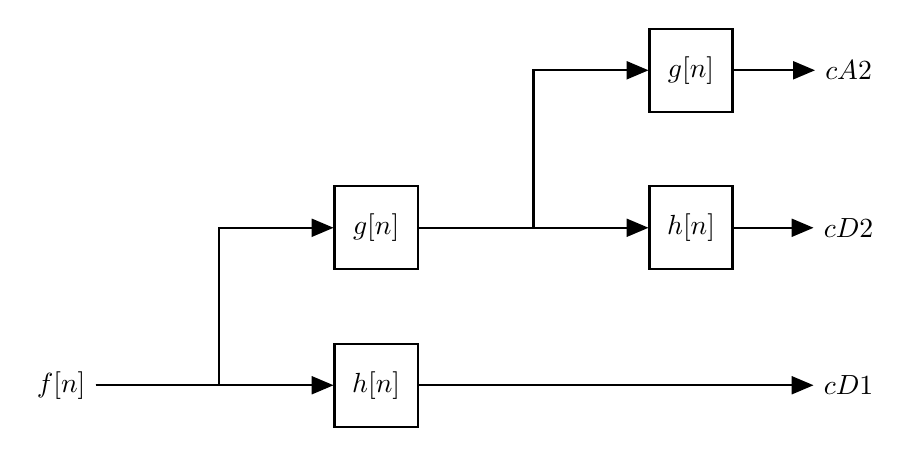
\begin{tikzpicture}[auto, thick, node distance=2cm, >=triangle 45]
\draw
	% Ebene 1
	node at (0,0)[name=in]{$f[n]$}
    node [input, right of=in](input1){}
	node [block, right of=input1] (h1) {$h[n]$}
	node [block, above of=h1] (g1) {$g[n]$}

	% Ebene 2
    node [input, right of=g1](input2){}
	node [block, right of=input2] (h2) {$h[n]$}
	node [block, above of=h2] (g2) {$g[n]$}

	% Ausgänge
    node [right of=g2](outg) {$cA2$}
    node [below of=outg](out2) {$cD2$}
    node [below of=out2](out1) {$cD1$}
;

    % Ebene 1
	\draw[->](in) -- node {}(h1);
	\draw[->](in) -- (input1) |- node {}(g1);
	\draw[->](h1) -- node {}(out1);

    % Ebene 2
	\draw[->](g1) -- node {}(h2);
	\draw[->](g1) -- (input2) |- node {}(g2);
	\draw[->](h2) -- node {}(out2);

	\draw[->](g2) -- node {}(outg);


\end{tikzpicture}
    \caption{Wavelet-Transformation als Filter\label{polynomials:filter}}
\end{figure}

Die Detailkoeffizienten auf Ebene $k$ entsprechen der Analyse mit einem $2^k$
skaliertem Mutterwavelet $\psi$ und die Approximationskoeffizienten der
entsprechenden Analyse mit einem Vaterwavelet $\varphi$.

Die Analysen und Simulationen wurden jeweils mittels Python~\cite{python} und im
speziellem dem PyWavelets~\cite{gregory_r_lee_2019_2634243} Paket durchgeführt.
Der dazu verwendete Code wurde in einem GitHub-Repository%
\footnote{\url{https://github.com/rnestler/mathsem-FS2019/tree/paper}}%
~\cite{polynomials:repo}
abgelegt. Zusätzlich sind auch interaktive Jupyter Notebooks abgelegt um den
Einfluss von verschiedenen Parametern auszuprobieren. Mittels
Binder%
\footnote{\url{https://mybinder.org/v2/gh/rnestler/mathsem-FS2019/paper}}%
~\cite{project_jupyter-proc-scipy-2018}
kann eine Online-Umgebung gestartet werden um diese Beispiele auszuführen.

\section{Analyse von polynomialen Signalen}
\rhead{Polynomiale Signale}

Wir werden als erstes die Signale in \autoref{polynomials:signals} mittels des db1
(Haar) Wavelets analysieren.

\begin{figure}
    \centering
    %% Creator: Matplotlib, PGF backend
%%
%% To include the figure in your LaTeX document, write
%%   \input{<filename>.pgf}
%%
%% Make sure the required packages are loaded in your preamble
%%   \usepackage{pgf}
%%
%% Figures using additional raster images can only be included by \input if
%% they are in the same directory as the main LaTeX file. For loading figures
%% from other directories you can use the `import` package
%%   \usepackage{import}
%% and then include the figures with
%%   \import{<path to file>}{<filename>.pgf}
%%
%% Matplotlib used the following preamble
%%   \usepackage{fontspec}
%%
\begingroup%
\makeatletter%
\begin{pgfpicture}%
\pgfpathrectangle{\pgfpointorigin}{\pgfqpoint{2.900000in}{3.000000in}}%
\pgfusepath{use as bounding box, clip}%
\begin{pgfscope}%
\pgfsetbuttcap%
\pgfsetmiterjoin%
\definecolor{currentfill}{rgb}{1.000000,1.000000,1.000000}%
\pgfsetfillcolor{currentfill}%
\pgfsetlinewidth{0.000000pt}%
\definecolor{currentstroke}{rgb}{1.000000,1.000000,1.000000}%
\pgfsetstrokecolor{currentstroke}%
\pgfsetdash{}{0pt}%
\pgfpathmoveto{\pgfqpoint{0.000000in}{0.000000in}}%
\pgfpathlineto{\pgfqpoint{2.900000in}{0.000000in}}%
\pgfpathlineto{\pgfqpoint{2.900000in}{3.000000in}}%
\pgfpathlineto{\pgfqpoint{0.000000in}{3.000000in}}%
\pgfpathclose%
\pgfusepath{fill}%
\end{pgfscope}%
\begin{pgfscope}%
\pgfsetbuttcap%
\pgfsetmiterjoin%
\definecolor{currentfill}{rgb}{1.000000,1.000000,1.000000}%
\pgfsetfillcolor{currentfill}%
\pgfsetlinewidth{0.000000pt}%
\definecolor{currentstroke}{rgb}{0.000000,0.000000,0.000000}%
\pgfsetstrokecolor{currentstroke}%
\pgfsetstrokeopacity{0.000000}%
\pgfsetdash{}{0pt}%
\pgfpathmoveto{\pgfqpoint{0.362500in}{0.375000in}}%
\pgfpathlineto{\pgfqpoint{2.610000in}{0.375000in}}%
\pgfpathlineto{\pgfqpoint{2.610000in}{2.640000in}}%
\pgfpathlineto{\pgfqpoint{0.362500in}{2.640000in}}%
\pgfpathclose%
\pgfusepath{fill}%
\end{pgfscope}%
\begin{pgfscope}%
\pgfsetbuttcap%
\pgfsetroundjoin%
\definecolor{currentfill}{rgb}{0.000000,0.000000,0.000000}%
\pgfsetfillcolor{currentfill}%
\pgfsetlinewidth{0.803000pt}%
\definecolor{currentstroke}{rgb}{0.000000,0.000000,0.000000}%
\pgfsetstrokecolor{currentstroke}%
\pgfsetdash{}{0pt}%
\pgfsys@defobject{currentmarker}{\pgfqpoint{0.000000in}{-0.048611in}}{\pgfqpoint{0.000000in}{0.000000in}}{%
\pgfpathmoveto{\pgfqpoint{0.000000in}{0.000000in}}%
\pgfpathlineto{\pgfqpoint{0.000000in}{-0.048611in}}%
\pgfusepath{stroke,fill}%
}%
\begin{pgfscope}%
\pgfsys@transformshift{0.464659in}{0.375000in}%
\pgfsys@useobject{currentmarker}{}%
\end{pgfscope}%
\end{pgfscope}%
\begin{pgfscope}%
\definecolor{textcolor}{rgb}{0.000000,0.000000,0.000000}%
\pgfsetstrokecolor{textcolor}%
\pgfsetfillcolor{textcolor}%
\pgftext[x=0.464659in,y=0.277778in,,top]{\color{textcolor}\rmfamily\fontsize{8.000000}{9.600000}\selectfont 0.0}%
\end{pgfscope}%
\begin{pgfscope}%
\pgfsetbuttcap%
\pgfsetroundjoin%
\definecolor{currentfill}{rgb}{0.000000,0.000000,0.000000}%
\pgfsetfillcolor{currentfill}%
\pgfsetlinewidth{0.803000pt}%
\definecolor{currentstroke}{rgb}{0.000000,0.000000,0.000000}%
\pgfsetstrokecolor{currentstroke}%
\pgfsetdash{}{0pt}%
\pgfsys@defobject{currentmarker}{\pgfqpoint{0.000000in}{-0.048611in}}{\pgfqpoint{0.000000in}{0.000000in}}{%
\pgfpathmoveto{\pgfqpoint{0.000000in}{0.000000in}}%
\pgfpathlineto{\pgfqpoint{0.000000in}{-0.048611in}}%
\pgfusepath{stroke,fill}%
}%
\begin{pgfscope}%
\pgfsys@transformshift{0.975455in}{0.375000in}%
\pgfsys@useobject{currentmarker}{}%
\end{pgfscope}%
\end{pgfscope}%
\begin{pgfscope}%
\definecolor{textcolor}{rgb}{0.000000,0.000000,0.000000}%
\pgfsetstrokecolor{textcolor}%
\pgfsetfillcolor{textcolor}%
\pgftext[x=0.975455in,y=0.277778in,,top]{\color{textcolor}\rmfamily\fontsize{8.000000}{9.600000}\selectfont 0.5}%
\end{pgfscope}%
\begin{pgfscope}%
\pgfsetbuttcap%
\pgfsetroundjoin%
\definecolor{currentfill}{rgb}{0.000000,0.000000,0.000000}%
\pgfsetfillcolor{currentfill}%
\pgfsetlinewidth{0.803000pt}%
\definecolor{currentstroke}{rgb}{0.000000,0.000000,0.000000}%
\pgfsetstrokecolor{currentstroke}%
\pgfsetdash{}{0pt}%
\pgfsys@defobject{currentmarker}{\pgfqpoint{0.000000in}{-0.048611in}}{\pgfqpoint{0.000000in}{0.000000in}}{%
\pgfpathmoveto{\pgfqpoint{0.000000in}{0.000000in}}%
\pgfpathlineto{\pgfqpoint{0.000000in}{-0.048611in}}%
\pgfusepath{stroke,fill}%
}%
\begin{pgfscope}%
\pgfsys@transformshift{1.486250in}{0.375000in}%
\pgfsys@useobject{currentmarker}{}%
\end{pgfscope}%
\end{pgfscope}%
\begin{pgfscope}%
\definecolor{textcolor}{rgb}{0.000000,0.000000,0.000000}%
\pgfsetstrokecolor{textcolor}%
\pgfsetfillcolor{textcolor}%
\pgftext[x=1.486250in,y=0.277778in,,top]{\color{textcolor}\rmfamily\fontsize{8.000000}{9.600000}\selectfont 1.0}%
\end{pgfscope}%
\begin{pgfscope}%
\pgfsetbuttcap%
\pgfsetroundjoin%
\definecolor{currentfill}{rgb}{0.000000,0.000000,0.000000}%
\pgfsetfillcolor{currentfill}%
\pgfsetlinewidth{0.803000pt}%
\definecolor{currentstroke}{rgb}{0.000000,0.000000,0.000000}%
\pgfsetstrokecolor{currentstroke}%
\pgfsetdash{}{0pt}%
\pgfsys@defobject{currentmarker}{\pgfqpoint{0.000000in}{-0.048611in}}{\pgfqpoint{0.000000in}{0.000000in}}{%
\pgfpathmoveto{\pgfqpoint{0.000000in}{0.000000in}}%
\pgfpathlineto{\pgfqpoint{0.000000in}{-0.048611in}}%
\pgfusepath{stroke,fill}%
}%
\begin{pgfscope}%
\pgfsys@transformshift{1.997045in}{0.375000in}%
\pgfsys@useobject{currentmarker}{}%
\end{pgfscope}%
\end{pgfscope}%
\begin{pgfscope}%
\definecolor{textcolor}{rgb}{0.000000,0.000000,0.000000}%
\pgfsetstrokecolor{textcolor}%
\pgfsetfillcolor{textcolor}%
\pgftext[x=1.997045in,y=0.277778in,,top]{\color{textcolor}\rmfamily\fontsize{8.000000}{9.600000}\selectfont 1.5}%
\end{pgfscope}%
\begin{pgfscope}%
\pgfsetbuttcap%
\pgfsetroundjoin%
\definecolor{currentfill}{rgb}{0.000000,0.000000,0.000000}%
\pgfsetfillcolor{currentfill}%
\pgfsetlinewidth{0.803000pt}%
\definecolor{currentstroke}{rgb}{0.000000,0.000000,0.000000}%
\pgfsetstrokecolor{currentstroke}%
\pgfsetdash{}{0pt}%
\pgfsys@defobject{currentmarker}{\pgfqpoint{0.000000in}{-0.048611in}}{\pgfqpoint{0.000000in}{0.000000in}}{%
\pgfpathmoveto{\pgfqpoint{0.000000in}{0.000000in}}%
\pgfpathlineto{\pgfqpoint{0.000000in}{-0.048611in}}%
\pgfusepath{stroke,fill}%
}%
\begin{pgfscope}%
\pgfsys@transformshift{2.507841in}{0.375000in}%
\pgfsys@useobject{currentmarker}{}%
\end{pgfscope}%
\end{pgfscope}%
\begin{pgfscope}%
\definecolor{textcolor}{rgb}{0.000000,0.000000,0.000000}%
\pgfsetstrokecolor{textcolor}%
\pgfsetfillcolor{textcolor}%
\pgftext[x=2.507841in,y=0.277778in,,top]{\color{textcolor}\rmfamily\fontsize{8.000000}{9.600000}\selectfont 2.0}%
\end{pgfscope}%
\begin{pgfscope}%
\pgfsetbuttcap%
\pgfsetroundjoin%
\definecolor{currentfill}{rgb}{0.000000,0.000000,0.000000}%
\pgfsetfillcolor{currentfill}%
\pgfsetlinewidth{0.803000pt}%
\definecolor{currentstroke}{rgb}{0.000000,0.000000,0.000000}%
\pgfsetstrokecolor{currentstroke}%
\pgfsetdash{}{0pt}%
\pgfsys@defobject{currentmarker}{\pgfqpoint{-0.048611in}{0.000000in}}{\pgfqpoint{0.000000in}{0.000000in}}{%
\pgfpathmoveto{\pgfqpoint{0.000000in}{0.000000in}}%
\pgfpathlineto{\pgfqpoint{-0.048611in}{0.000000in}}%
\pgfusepath{stroke,fill}%
}%
\begin{pgfscope}%
\pgfsys@transformshift{0.362500in}{0.477955in}%
\pgfsys@useobject{currentmarker}{}%
\end{pgfscope}%
\end{pgfscope}%
\begin{pgfscope}%
\definecolor{textcolor}{rgb}{0.000000,0.000000,0.000000}%
\pgfsetstrokecolor{textcolor}%
\pgfsetfillcolor{textcolor}%
\pgftext[x=0.206278in,y=0.439399in,left,base]{\color{textcolor}\rmfamily\fontsize{8.000000}{9.600000}\selectfont 0}%
\end{pgfscope}%
\begin{pgfscope}%
\pgfsetbuttcap%
\pgfsetroundjoin%
\definecolor{currentfill}{rgb}{0.000000,0.000000,0.000000}%
\pgfsetfillcolor{currentfill}%
\pgfsetlinewidth{0.803000pt}%
\definecolor{currentstroke}{rgb}{0.000000,0.000000,0.000000}%
\pgfsetstrokecolor{currentstroke}%
\pgfsetdash{}{0pt}%
\pgfsys@defobject{currentmarker}{\pgfqpoint{-0.048611in}{0.000000in}}{\pgfqpoint{0.000000in}{0.000000in}}{%
\pgfpathmoveto{\pgfqpoint{0.000000in}{0.000000in}}%
\pgfpathlineto{\pgfqpoint{-0.048611in}{0.000000in}}%
\pgfusepath{stroke,fill}%
}%
\begin{pgfscope}%
\pgfsys@transformshift{0.362500in}{0.735341in}%
\pgfsys@useobject{currentmarker}{}%
\end{pgfscope}%
\end{pgfscope}%
\begin{pgfscope}%
\definecolor{textcolor}{rgb}{0.000000,0.000000,0.000000}%
\pgfsetstrokecolor{textcolor}%
\pgfsetfillcolor{textcolor}%
\pgftext[x=0.206278in,y=0.696785in,left,base]{\color{textcolor}\rmfamily\fontsize{8.000000}{9.600000}\selectfont 1}%
\end{pgfscope}%
\begin{pgfscope}%
\pgfsetbuttcap%
\pgfsetroundjoin%
\definecolor{currentfill}{rgb}{0.000000,0.000000,0.000000}%
\pgfsetfillcolor{currentfill}%
\pgfsetlinewidth{0.803000pt}%
\definecolor{currentstroke}{rgb}{0.000000,0.000000,0.000000}%
\pgfsetstrokecolor{currentstroke}%
\pgfsetdash{}{0pt}%
\pgfsys@defobject{currentmarker}{\pgfqpoint{-0.048611in}{0.000000in}}{\pgfqpoint{0.000000in}{0.000000in}}{%
\pgfpathmoveto{\pgfqpoint{0.000000in}{0.000000in}}%
\pgfpathlineto{\pgfqpoint{-0.048611in}{0.000000in}}%
\pgfusepath{stroke,fill}%
}%
\begin{pgfscope}%
\pgfsys@transformshift{0.362500in}{0.992727in}%
\pgfsys@useobject{currentmarker}{}%
\end{pgfscope}%
\end{pgfscope}%
\begin{pgfscope}%
\definecolor{textcolor}{rgb}{0.000000,0.000000,0.000000}%
\pgfsetstrokecolor{textcolor}%
\pgfsetfillcolor{textcolor}%
\pgftext[x=0.206278in,y=0.954172in,left,base]{\color{textcolor}\rmfamily\fontsize{8.000000}{9.600000}\selectfont 2}%
\end{pgfscope}%
\begin{pgfscope}%
\pgfsetbuttcap%
\pgfsetroundjoin%
\definecolor{currentfill}{rgb}{0.000000,0.000000,0.000000}%
\pgfsetfillcolor{currentfill}%
\pgfsetlinewidth{0.803000pt}%
\definecolor{currentstroke}{rgb}{0.000000,0.000000,0.000000}%
\pgfsetstrokecolor{currentstroke}%
\pgfsetdash{}{0pt}%
\pgfsys@defobject{currentmarker}{\pgfqpoint{-0.048611in}{0.000000in}}{\pgfqpoint{0.000000in}{0.000000in}}{%
\pgfpathmoveto{\pgfqpoint{0.000000in}{0.000000in}}%
\pgfpathlineto{\pgfqpoint{-0.048611in}{0.000000in}}%
\pgfusepath{stroke,fill}%
}%
\begin{pgfscope}%
\pgfsys@transformshift{0.362500in}{1.250114in}%
\pgfsys@useobject{currentmarker}{}%
\end{pgfscope}%
\end{pgfscope}%
\begin{pgfscope}%
\definecolor{textcolor}{rgb}{0.000000,0.000000,0.000000}%
\pgfsetstrokecolor{textcolor}%
\pgfsetfillcolor{textcolor}%
\pgftext[x=0.206278in,y=1.211558in,left,base]{\color{textcolor}\rmfamily\fontsize{8.000000}{9.600000}\selectfont 3}%
\end{pgfscope}%
\begin{pgfscope}%
\pgfsetbuttcap%
\pgfsetroundjoin%
\definecolor{currentfill}{rgb}{0.000000,0.000000,0.000000}%
\pgfsetfillcolor{currentfill}%
\pgfsetlinewidth{0.803000pt}%
\definecolor{currentstroke}{rgb}{0.000000,0.000000,0.000000}%
\pgfsetstrokecolor{currentstroke}%
\pgfsetdash{}{0pt}%
\pgfsys@defobject{currentmarker}{\pgfqpoint{-0.048611in}{0.000000in}}{\pgfqpoint{0.000000in}{0.000000in}}{%
\pgfpathmoveto{\pgfqpoint{0.000000in}{0.000000in}}%
\pgfpathlineto{\pgfqpoint{-0.048611in}{0.000000in}}%
\pgfusepath{stroke,fill}%
}%
\begin{pgfscope}%
\pgfsys@transformshift{0.362500in}{1.507500in}%
\pgfsys@useobject{currentmarker}{}%
\end{pgfscope}%
\end{pgfscope}%
\begin{pgfscope}%
\definecolor{textcolor}{rgb}{0.000000,0.000000,0.000000}%
\pgfsetstrokecolor{textcolor}%
\pgfsetfillcolor{textcolor}%
\pgftext[x=0.206278in,y=1.468944in,left,base]{\color{textcolor}\rmfamily\fontsize{8.000000}{9.600000}\selectfont 4}%
\end{pgfscope}%
\begin{pgfscope}%
\pgfsetbuttcap%
\pgfsetroundjoin%
\definecolor{currentfill}{rgb}{0.000000,0.000000,0.000000}%
\pgfsetfillcolor{currentfill}%
\pgfsetlinewidth{0.803000pt}%
\definecolor{currentstroke}{rgb}{0.000000,0.000000,0.000000}%
\pgfsetstrokecolor{currentstroke}%
\pgfsetdash{}{0pt}%
\pgfsys@defobject{currentmarker}{\pgfqpoint{-0.048611in}{0.000000in}}{\pgfqpoint{0.000000in}{0.000000in}}{%
\pgfpathmoveto{\pgfqpoint{0.000000in}{0.000000in}}%
\pgfpathlineto{\pgfqpoint{-0.048611in}{0.000000in}}%
\pgfusepath{stroke,fill}%
}%
\begin{pgfscope}%
\pgfsys@transformshift{0.362500in}{1.764886in}%
\pgfsys@useobject{currentmarker}{}%
\end{pgfscope}%
\end{pgfscope}%
\begin{pgfscope}%
\definecolor{textcolor}{rgb}{0.000000,0.000000,0.000000}%
\pgfsetstrokecolor{textcolor}%
\pgfsetfillcolor{textcolor}%
\pgftext[x=0.206278in,y=1.726331in,left,base]{\color{textcolor}\rmfamily\fontsize{8.000000}{9.600000}\selectfont 5}%
\end{pgfscope}%
\begin{pgfscope}%
\pgfsetbuttcap%
\pgfsetroundjoin%
\definecolor{currentfill}{rgb}{0.000000,0.000000,0.000000}%
\pgfsetfillcolor{currentfill}%
\pgfsetlinewidth{0.803000pt}%
\definecolor{currentstroke}{rgb}{0.000000,0.000000,0.000000}%
\pgfsetstrokecolor{currentstroke}%
\pgfsetdash{}{0pt}%
\pgfsys@defobject{currentmarker}{\pgfqpoint{-0.048611in}{0.000000in}}{\pgfqpoint{0.000000in}{0.000000in}}{%
\pgfpathmoveto{\pgfqpoint{0.000000in}{0.000000in}}%
\pgfpathlineto{\pgfqpoint{-0.048611in}{0.000000in}}%
\pgfusepath{stroke,fill}%
}%
\begin{pgfscope}%
\pgfsys@transformshift{0.362500in}{2.022273in}%
\pgfsys@useobject{currentmarker}{}%
\end{pgfscope}%
\end{pgfscope}%
\begin{pgfscope}%
\definecolor{textcolor}{rgb}{0.000000,0.000000,0.000000}%
\pgfsetstrokecolor{textcolor}%
\pgfsetfillcolor{textcolor}%
\pgftext[x=0.206278in,y=1.983717in,left,base]{\color{textcolor}\rmfamily\fontsize{8.000000}{9.600000}\selectfont 6}%
\end{pgfscope}%
\begin{pgfscope}%
\pgfsetbuttcap%
\pgfsetroundjoin%
\definecolor{currentfill}{rgb}{0.000000,0.000000,0.000000}%
\pgfsetfillcolor{currentfill}%
\pgfsetlinewidth{0.803000pt}%
\definecolor{currentstroke}{rgb}{0.000000,0.000000,0.000000}%
\pgfsetstrokecolor{currentstroke}%
\pgfsetdash{}{0pt}%
\pgfsys@defobject{currentmarker}{\pgfqpoint{-0.048611in}{0.000000in}}{\pgfqpoint{0.000000in}{0.000000in}}{%
\pgfpathmoveto{\pgfqpoint{0.000000in}{0.000000in}}%
\pgfpathlineto{\pgfqpoint{-0.048611in}{0.000000in}}%
\pgfusepath{stroke,fill}%
}%
\begin{pgfscope}%
\pgfsys@transformshift{0.362500in}{2.279659in}%
\pgfsys@useobject{currentmarker}{}%
\end{pgfscope}%
\end{pgfscope}%
\begin{pgfscope}%
\definecolor{textcolor}{rgb}{0.000000,0.000000,0.000000}%
\pgfsetstrokecolor{textcolor}%
\pgfsetfillcolor{textcolor}%
\pgftext[x=0.206278in,y=2.241104in,left,base]{\color{textcolor}\rmfamily\fontsize{8.000000}{9.600000}\selectfont 7}%
\end{pgfscope}%
\begin{pgfscope}%
\pgfsetbuttcap%
\pgfsetroundjoin%
\definecolor{currentfill}{rgb}{0.000000,0.000000,0.000000}%
\pgfsetfillcolor{currentfill}%
\pgfsetlinewidth{0.803000pt}%
\definecolor{currentstroke}{rgb}{0.000000,0.000000,0.000000}%
\pgfsetstrokecolor{currentstroke}%
\pgfsetdash{}{0pt}%
\pgfsys@defobject{currentmarker}{\pgfqpoint{-0.048611in}{0.000000in}}{\pgfqpoint{0.000000in}{0.000000in}}{%
\pgfpathmoveto{\pgfqpoint{0.000000in}{0.000000in}}%
\pgfpathlineto{\pgfqpoint{-0.048611in}{0.000000in}}%
\pgfusepath{stroke,fill}%
}%
\begin{pgfscope}%
\pgfsys@transformshift{0.362500in}{2.537045in}%
\pgfsys@useobject{currentmarker}{}%
\end{pgfscope}%
\end{pgfscope}%
\begin{pgfscope}%
\definecolor{textcolor}{rgb}{0.000000,0.000000,0.000000}%
\pgfsetstrokecolor{textcolor}%
\pgfsetfillcolor{textcolor}%
\pgftext[x=0.206278in,y=2.498490in,left,base]{\color{textcolor}\rmfamily\fontsize{8.000000}{9.600000}\selectfont 8}%
\end{pgfscope}%
\begin{pgfscope}%
\pgfpathrectangle{\pgfqpoint{0.362500in}{0.375000in}}{\pgfqpoint{2.247500in}{2.265000in}}%
\pgfusepath{clip}%
\pgfsetrectcap%
\pgfsetroundjoin%
\pgfsetlinewidth{1.505625pt}%
\definecolor{currentstroke}{rgb}{0.121569,0.466667,0.705882}%
\pgfsetstrokecolor{currentstroke}%
\pgfsetdash{}{0pt}%
\pgfpathmoveto{\pgfqpoint{0.464659in}{0.477955in}}%
\pgfpathlineto{\pgfqpoint{0.472672in}{0.500749in}}%
\pgfpathlineto{\pgfqpoint{0.488697in}{0.517436in}}%
\pgfpathlineto{\pgfqpoint{0.504721in}{0.528925in}}%
\pgfpathlineto{\pgfqpoint{0.528759in}{0.542427in}}%
\pgfpathlineto{\pgfqpoint{0.560809in}{0.556917in}}%
\pgfpathlineto{\pgfqpoint{0.608884in}{0.574664in}}%
\pgfpathlineto{\pgfqpoint{0.664971in}{0.591927in}}%
\pgfpathlineto{\pgfqpoint{0.737083in}{0.610868in}}%
\pgfpathlineto{\pgfqpoint{0.825221in}{0.630865in}}%
\pgfpathlineto{\pgfqpoint{0.937395in}{0.653043in}}%
\pgfpathlineto{\pgfqpoint{1.073607in}{0.676673in}}%
\pgfpathlineto{\pgfqpoint{1.233857in}{0.701294in}}%
\pgfpathlineto{\pgfqpoint{1.426156in}{0.727656in}}%
\pgfpathlineto{\pgfqpoint{1.650506in}{0.755262in}}%
\pgfpathlineto{\pgfqpoint{1.914918in}{0.784623in}}%
\pgfpathlineto{\pgfqpoint{2.219392in}{0.815283in}}%
\pgfpathlineto{\pgfqpoint{2.507841in}{0.841954in}}%
\pgfpathlineto{\pgfqpoint{2.507841in}{0.841954in}}%
\pgfusepath{stroke}%
\end{pgfscope}%
\begin{pgfscope}%
\pgfpathrectangle{\pgfqpoint{0.362500in}{0.375000in}}{\pgfqpoint{2.247500in}{2.265000in}}%
\pgfusepath{clip}%
\pgfsetrectcap%
\pgfsetroundjoin%
\pgfsetlinewidth{1.505625pt}%
\definecolor{currentstroke}{rgb}{1.000000,0.498039,0.054902}%
\pgfsetstrokecolor{currentstroke}%
\pgfsetdash{}{0pt}%
\pgfpathmoveto{\pgfqpoint{0.464659in}{0.735341in}}%
\pgfpathlineto{\pgfqpoint{2.507841in}{0.735341in}}%
\pgfpathlineto{\pgfqpoint{2.507841in}{0.735341in}}%
\pgfusepath{stroke}%
\end{pgfscope}%
\begin{pgfscope}%
\pgfpathrectangle{\pgfqpoint{0.362500in}{0.375000in}}{\pgfqpoint{2.247500in}{2.265000in}}%
\pgfusepath{clip}%
\pgfsetrectcap%
\pgfsetroundjoin%
\pgfsetlinewidth{1.505625pt}%
\definecolor{currentstroke}{rgb}{0.172549,0.627451,0.172549}%
\pgfsetstrokecolor{currentstroke}%
\pgfsetdash{}{0pt}%
\pgfpathmoveto{\pgfqpoint{0.464659in}{0.477955in}}%
\pgfpathlineto{\pgfqpoint{2.507841in}{0.992727in}}%
\pgfpathlineto{\pgfqpoint{2.507841in}{0.992727in}}%
\pgfusepath{stroke}%
\end{pgfscope}%
\begin{pgfscope}%
\pgfpathrectangle{\pgfqpoint{0.362500in}{0.375000in}}{\pgfqpoint{2.247500in}{2.265000in}}%
\pgfusepath{clip}%
\pgfsetrectcap%
\pgfsetroundjoin%
\pgfsetlinewidth{1.505625pt}%
\definecolor{currentstroke}{rgb}{0.839216,0.152941,0.156863}%
\pgfsetstrokecolor{currentstroke}%
\pgfsetdash{}{0pt}%
\pgfpathmoveto{\pgfqpoint{0.464659in}{0.477955in}}%
\pgfpathlineto{\pgfqpoint{0.544784in}{0.479538in}}%
\pgfpathlineto{\pgfqpoint{0.624909in}{0.484288in}}%
\pgfpathlineto{\pgfqpoint{0.705033in}{0.492204in}}%
\pgfpathlineto{\pgfqpoint{0.785158in}{0.503287in}}%
\pgfpathlineto{\pgfqpoint{0.865283in}{0.517537in}}%
\pgfpathlineto{\pgfqpoint{0.945408in}{0.534954in}}%
\pgfpathlineto{\pgfqpoint{1.025533in}{0.555537in}}%
\pgfpathlineto{\pgfqpoint{1.105657in}{0.579286in}}%
\pgfpathlineto{\pgfqpoint{1.185782in}{0.606202in}}%
\pgfpathlineto{\pgfqpoint{1.265907in}{0.636285in}}%
\pgfpathlineto{\pgfqpoint{1.346032in}{0.669535in}}%
\pgfpathlineto{\pgfqpoint{1.426156in}{0.705951in}}%
\pgfpathlineto{\pgfqpoint{1.506281in}{0.745533in}}%
\pgfpathlineto{\pgfqpoint{1.586406in}{0.788283in}}%
\pgfpathlineto{\pgfqpoint{1.674543in}{0.838964in}}%
\pgfpathlineto{\pgfqpoint{1.762680in}{0.893478in}}%
\pgfpathlineto{\pgfqpoint{1.850818in}{0.951823in}}%
\pgfpathlineto{\pgfqpoint{1.938955in}{1.013999in}}%
\pgfpathlineto{\pgfqpoint{2.027092in}{1.080007in}}%
\pgfpathlineto{\pgfqpoint{2.115230in}{1.149847in}}%
\pgfpathlineto{\pgfqpoint{2.203367in}{1.223518in}}%
\pgfpathlineto{\pgfqpoint{2.291504in}{1.301021in}}%
\pgfpathlineto{\pgfqpoint{2.379641in}{1.382355in}}%
\pgfpathlineto{\pgfqpoint{2.475791in}{1.475454in}}%
\pgfpathlineto{\pgfqpoint{2.507841in}{1.507500in}}%
\pgfpathlineto{\pgfqpoint{2.507841in}{1.507500in}}%
\pgfusepath{stroke}%
\end{pgfscope}%
\begin{pgfscope}%
\pgfpathrectangle{\pgfqpoint{0.362500in}{0.375000in}}{\pgfqpoint{2.247500in}{2.265000in}}%
\pgfusepath{clip}%
\pgfsetrectcap%
\pgfsetroundjoin%
\pgfsetlinewidth{1.505625pt}%
\definecolor{currentstroke}{rgb}{0.580392,0.403922,0.741176}%
\pgfsetstrokecolor{currentstroke}%
\pgfsetdash{}{0pt}%
\pgfpathmoveto{\pgfqpoint{0.464659in}{0.477955in}}%
\pgfpathlineto{\pgfqpoint{0.648946in}{0.479465in}}%
\pgfpathlineto{\pgfqpoint{0.745096in}{0.483279in}}%
\pgfpathlineto{\pgfqpoint{0.825221in}{0.489271in}}%
\pgfpathlineto{\pgfqpoint{0.897333in}{0.497509in}}%
\pgfpathlineto{\pgfqpoint{0.969445in}{0.509006in}}%
\pgfpathlineto{\pgfqpoint{1.033545in}{0.522400in}}%
\pgfpathlineto{\pgfqpoint{1.097645in}{0.539181in}}%
\pgfpathlineto{\pgfqpoint{1.153732in}{0.556941in}}%
\pgfpathlineto{\pgfqpoint{1.209820in}{0.577840in}}%
\pgfpathlineto{\pgfqpoint{1.265907in}{0.602135in}}%
\pgfpathlineto{\pgfqpoint{1.321994in}{0.630082in}}%
\pgfpathlineto{\pgfqpoint{1.378082in}{0.661934in}}%
\pgfpathlineto{\pgfqpoint{1.426156in}{0.692539in}}%
\pgfpathlineto{\pgfqpoint{1.474231in}{0.726363in}}%
\pgfpathlineto{\pgfqpoint{1.522306in}{0.763567in}}%
\pgfpathlineto{\pgfqpoint{1.570381in}{0.804311in}}%
\pgfpathlineto{\pgfqpoint{1.618456in}{0.848757in}}%
\pgfpathlineto{\pgfqpoint{1.666531in}{0.897065in}}%
\pgfpathlineto{\pgfqpoint{1.714606in}{0.949397in}}%
\pgfpathlineto{\pgfqpoint{1.762680in}{1.005913in}}%
\pgfpathlineto{\pgfqpoint{1.810755in}{1.066775in}}%
\pgfpathlineto{\pgfqpoint{1.858830in}{1.132143in}}%
\pgfpathlineto{\pgfqpoint{1.906905in}{1.202178in}}%
\pgfpathlineto{\pgfqpoint{1.954980in}{1.277041in}}%
\pgfpathlineto{\pgfqpoint{2.003055in}{1.356893in}}%
\pgfpathlineto{\pgfqpoint{2.059142in}{1.456575in}}%
\pgfpathlineto{\pgfqpoint{2.115230in}{1.563522in}}%
\pgfpathlineto{\pgfqpoint{2.171317in}{1.677989in}}%
\pgfpathlineto{\pgfqpoint{2.227404in}{1.800233in}}%
\pgfpathlineto{\pgfqpoint{2.283492in}{1.930509in}}%
\pgfpathlineto{\pgfqpoint{2.339579in}{2.069073in}}%
\pgfpathlineto{\pgfqpoint{2.395666in}{2.216180in}}%
\pgfpathlineto{\pgfqpoint{2.451754in}{2.372086in}}%
\pgfpathlineto{\pgfqpoint{2.507841in}{2.537045in}}%
\pgfpathlineto{\pgfqpoint{2.507841in}{2.537045in}}%
\pgfusepath{stroke}%
\end{pgfscope}%
\begin{pgfscope}%
\pgfsetrectcap%
\pgfsetmiterjoin%
\pgfsetlinewidth{0.803000pt}%
\definecolor{currentstroke}{rgb}{0.000000,0.000000,0.000000}%
\pgfsetstrokecolor{currentstroke}%
\pgfsetdash{}{0pt}%
\pgfpathmoveto{\pgfqpoint{0.362500in}{0.375000in}}%
\pgfpathlineto{\pgfqpoint{0.362500in}{2.640000in}}%
\pgfusepath{stroke}%
\end{pgfscope}%
\begin{pgfscope}%
\pgfsetrectcap%
\pgfsetmiterjoin%
\pgfsetlinewidth{0.803000pt}%
\definecolor{currentstroke}{rgb}{0.000000,0.000000,0.000000}%
\pgfsetstrokecolor{currentstroke}%
\pgfsetdash{}{0pt}%
\pgfpathmoveto{\pgfqpoint{2.610000in}{0.375000in}}%
\pgfpathlineto{\pgfqpoint{2.610000in}{2.640000in}}%
\pgfusepath{stroke}%
\end{pgfscope}%
\begin{pgfscope}%
\pgfsetrectcap%
\pgfsetmiterjoin%
\pgfsetlinewidth{0.803000pt}%
\definecolor{currentstroke}{rgb}{0.000000,0.000000,0.000000}%
\pgfsetstrokecolor{currentstroke}%
\pgfsetdash{}{0pt}%
\pgfpathmoveto{\pgfqpoint{0.362500in}{0.375000in}}%
\pgfpathlineto{\pgfqpoint{2.610000in}{0.375000in}}%
\pgfusepath{stroke}%
\end{pgfscope}%
\begin{pgfscope}%
\pgfsetrectcap%
\pgfsetmiterjoin%
\pgfsetlinewidth{0.803000pt}%
\definecolor{currentstroke}{rgb}{0.000000,0.000000,0.000000}%
\pgfsetstrokecolor{currentstroke}%
\pgfsetdash{}{0pt}%
\pgfpathmoveto{\pgfqpoint{0.362500in}{2.640000in}}%
\pgfpathlineto{\pgfqpoint{2.610000in}{2.640000in}}%
\pgfusepath{stroke}%
\end{pgfscope}%
\begin{pgfscope}%
\pgfsetbuttcap%
\pgfsetmiterjoin%
\definecolor{currentfill}{rgb}{1.000000,1.000000,1.000000}%
\pgfsetfillcolor{currentfill}%
\pgfsetfillopacity{0.800000}%
\pgfsetlinewidth{1.003750pt}%
\definecolor{currentstroke}{rgb}{0.800000,0.800000,0.800000}%
\pgfsetstrokecolor{currentstroke}%
\pgfsetstrokeopacity{0.800000}%
\pgfsetdash{}{0pt}%
\pgfpathmoveto{\pgfqpoint{0.440278in}{1.774028in}}%
\pgfpathlineto{\pgfqpoint{1.002719in}{1.774028in}}%
\pgfpathquadraticcurveto{\pgfqpoint{1.024941in}{1.774028in}}{\pgfqpoint{1.024941in}{1.796251in}}%
\pgfpathlineto{\pgfqpoint{1.024941in}{2.562222in}}%
\pgfpathquadraticcurveto{\pgfqpoint{1.024941in}{2.584444in}}{\pgfqpoint{1.002719in}{2.584444in}}%
\pgfpathlineto{\pgfqpoint{0.440278in}{2.584444in}}%
\pgfpathquadraticcurveto{\pgfqpoint{0.418056in}{2.584444in}}{\pgfqpoint{0.418056in}{2.562222in}}%
\pgfpathlineto{\pgfqpoint{0.418056in}{1.796251in}}%
\pgfpathquadraticcurveto{\pgfqpoint{0.418056in}{1.774028in}}{\pgfqpoint{0.440278in}{1.774028in}}%
\pgfpathclose%
\pgfusepath{stroke,fill}%
\end{pgfscope}%
\begin{pgfscope}%
\pgfsetrectcap%
\pgfsetroundjoin%
\pgfsetlinewidth{1.505625pt}%
\definecolor{currentstroke}{rgb}{0.121569,0.466667,0.705882}%
\pgfsetstrokecolor{currentstroke}%
\pgfsetdash{}{0pt}%
\pgfpathmoveto{\pgfqpoint{0.462500in}{2.500583in}}%
\pgfpathlineto{\pgfqpoint{0.684722in}{2.500583in}}%
\pgfusepath{stroke}%
\end{pgfscope}%
\begin{pgfscope}%
\definecolor{textcolor}{rgb}{0.000000,0.000000,0.000000}%
\pgfsetstrokecolor{textcolor}%
\pgfsetfillcolor{textcolor}%
\pgftext[x=0.773611in,y=2.461694in,left,base]{\color{textcolor}\rmfamily\fontsize{8.000000}{9.600000}\selectfont \(\displaystyle x^{0.5}\)}%
\end{pgfscope}%
\begin{pgfscope}%
\pgfsetrectcap%
\pgfsetroundjoin%
\pgfsetlinewidth{1.505625pt}%
\definecolor{currentstroke}{rgb}{1.000000,0.498039,0.054902}%
\pgfsetstrokecolor{currentstroke}%
\pgfsetdash{}{0pt}%
\pgfpathmoveto{\pgfqpoint{0.462500in}{2.345167in}}%
\pgfpathlineto{\pgfqpoint{0.684722in}{2.345167in}}%
\pgfusepath{stroke}%
\end{pgfscope}%
\begin{pgfscope}%
\definecolor{textcolor}{rgb}{0.000000,0.000000,0.000000}%
\pgfsetstrokecolor{textcolor}%
\pgfsetfillcolor{textcolor}%
\pgftext[x=0.773611in,y=2.306278in,left,base]{\color{textcolor}\rmfamily\fontsize{8.000000}{9.600000}\selectfont \(\displaystyle x^{0}\)}%
\end{pgfscope}%
\begin{pgfscope}%
\pgfsetrectcap%
\pgfsetroundjoin%
\pgfsetlinewidth{1.505625pt}%
\definecolor{currentstroke}{rgb}{0.172549,0.627451,0.172549}%
\pgfsetstrokecolor{currentstroke}%
\pgfsetdash{}{0pt}%
\pgfpathmoveto{\pgfqpoint{0.462500in}{2.189750in}}%
\pgfpathlineto{\pgfqpoint{0.684722in}{2.189750in}}%
\pgfusepath{stroke}%
\end{pgfscope}%
\begin{pgfscope}%
\definecolor{textcolor}{rgb}{0.000000,0.000000,0.000000}%
\pgfsetstrokecolor{textcolor}%
\pgfsetfillcolor{textcolor}%
\pgftext[x=0.773611in,y=2.150861in,left,base]{\color{textcolor}\rmfamily\fontsize{8.000000}{9.600000}\selectfont \(\displaystyle x^{1}\)}%
\end{pgfscope}%
\begin{pgfscope}%
\pgfsetrectcap%
\pgfsetroundjoin%
\pgfsetlinewidth{1.505625pt}%
\definecolor{currentstroke}{rgb}{0.839216,0.152941,0.156863}%
\pgfsetstrokecolor{currentstroke}%
\pgfsetdash{}{0pt}%
\pgfpathmoveto{\pgfqpoint{0.462500in}{2.034334in}}%
\pgfpathlineto{\pgfqpoint{0.684722in}{2.034334in}}%
\pgfusepath{stroke}%
\end{pgfscope}%
\begin{pgfscope}%
\definecolor{textcolor}{rgb}{0.000000,0.000000,0.000000}%
\pgfsetstrokecolor{textcolor}%
\pgfsetfillcolor{textcolor}%
\pgftext[x=0.773611in,y=1.995445in,left,base]{\color{textcolor}\rmfamily\fontsize{8.000000}{9.600000}\selectfont \(\displaystyle x^{2}\)}%
\end{pgfscope}%
\begin{pgfscope}%
\pgfsetrectcap%
\pgfsetroundjoin%
\pgfsetlinewidth{1.505625pt}%
\definecolor{currentstroke}{rgb}{0.580392,0.403922,0.741176}%
\pgfsetstrokecolor{currentstroke}%
\pgfsetdash{}{0pt}%
\pgfpathmoveto{\pgfqpoint{0.462500in}{1.878917in}}%
\pgfpathlineto{\pgfqpoint{0.684722in}{1.878917in}}%
\pgfusepath{stroke}%
\end{pgfscope}%
\begin{pgfscope}%
\definecolor{textcolor}{rgb}{0.000000,0.000000,0.000000}%
\pgfsetstrokecolor{textcolor}%
\pgfsetfillcolor{textcolor}%
\pgftext[x=0.773611in,y=1.840028in,left,base]{\color{textcolor}\rmfamily\fontsize{8.000000}{9.600000}\selectfont \(\displaystyle x^{3}\)}%
\end{pgfscope}%
\end{pgfpicture}%
\makeatother%
\endgroup%

    \caption{Die verschiedenen zu analysierenden polynomialen Signale\label{polynomials:signals}}
\end{figure}

In~\autoref{polynomials:haar} sind die Approximations- und die Detailkoeffizienten
der Transformation zu sehen. Wir sehen, dass die Approximationskoeffizienten
uns das grobe Signal und im Fall von $x^0 = 1$ sogar das exakte Signal liefern. Die
Detailkoeffizienten scheinen uns etwas zu liefern was proportional zur ersten
Ableitung des Signals ist.

\begin{figure}
    \centering
    %% Creator: Matplotlib, PGF backend
%%
%% To include the figure in your LaTeX document, write
%%   \input{<filename>.pgf}
%%
%% Make sure the required packages are loaded in your preamble
%%   \usepackage{pgf}
%%
%% Figures using additional raster images can only be included by \input if
%% they are in the same directory as the main LaTeX file. For loading figures
%% from other directories you can use the `import` package
%%   \usepackage{import}
%% and then include the figures with
%%   \import{<path to file>}{<filename>.pgf}
%%
%% Matplotlib used the following preamble
%%   \usepackage{fontspec}
%%
\begingroup%
\makeatletter%
\begin{pgfpicture}%
\pgfpathrectangle{\pgfpointorigin}{\pgfqpoint{5.800000in}{3.300000in}}%
\pgfusepath{use as bounding box, clip}%
\begin{pgfscope}%
\pgfsetbuttcap%
\pgfsetmiterjoin%
\definecolor{currentfill}{rgb}{1.000000,1.000000,1.000000}%
\pgfsetfillcolor{currentfill}%
\pgfsetlinewidth{0.000000pt}%
\definecolor{currentstroke}{rgb}{1.000000,1.000000,1.000000}%
\pgfsetstrokecolor{currentstroke}%
\pgfsetdash{}{0pt}%
\pgfpathmoveto{\pgfqpoint{0.000000in}{0.000000in}}%
\pgfpathlineto{\pgfqpoint{5.800000in}{0.000000in}}%
\pgfpathlineto{\pgfqpoint{5.800000in}{3.300000in}}%
\pgfpathlineto{\pgfqpoint{0.000000in}{3.300000in}}%
\pgfpathclose%
\pgfusepath{fill}%
\end{pgfscope}%
\begin{pgfscope}%
\pgfsetbuttcap%
\pgfsetmiterjoin%
\definecolor{currentfill}{rgb}{1.000000,1.000000,1.000000}%
\pgfsetfillcolor{currentfill}%
\pgfsetlinewidth{0.000000pt}%
\definecolor{currentstroke}{rgb}{0.000000,0.000000,0.000000}%
\pgfsetstrokecolor{currentstroke}%
\pgfsetstrokeopacity{0.000000}%
\pgfsetdash{}{0pt}%
\pgfpathmoveto{\pgfqpoint{0.670972in}{1.861111in}}%
\pgfpathlineto{\pgfqpoint{4.930000in}{1.861111in}}%
\pgfpathlineto{\pgfqpoint{4.930000in}{2.926667in}}%
\pgfpathlineto{\pgfqpoint{0.670972in}{2.926667in}}%
\pgfpathclose%
\pgfusepath{fill}%
\end{pgfscope}%
\begin{pgfscope}%
\pgfsetbuttcap%
\pgfsetroundjoin%
\definecolor{currentfill}{rgb}{0.000000,0.000000,0.000000}%
\pgfsetfillcolor{currentfill}%
\pgfsetlinewidth{0.803000pt}%
\definecolor{currentstroke}{rgb}{0.000000,0.000000,0.000000}%
\pgfsetstrokecolor{currentstroke}%
\pgfsetdash{}{0pt}%
\pgfsys@defobject{currentmarker}{\pgfqpoint{0.000000in}{-0.048611in}}{\pgfqpoint{0.000000in}{0.000000in}}{%
\pgfpathmoveto{\pgfqpoint{0.000000in}{0.000000in}}%
\pgfpathlineto{\pgfqpoint{0.000000in}{-0.048611in}}%
\pgfusepath{stroke,fill}%
}%
\begin{pgfscope}%
\pgfsys@transformshift{0.864564in}{1.861111in}%
\pgfsys@useobject{currentmarker}{}%
\end{pgfscope}%
\end{pgfscope}%
\begin{pgfscope}%
\pgfsetbuttcap%
\pgfsetroundjoin%
\definecolor{currentfill}{rgb}{0.000000,0.000000,0.000000}%
\pgfsetfillcolor{currentfill}%
\pgfsetlinewidth{0.803000pt}%
\definecolor{currentstroke}{rgb}{0.000000,0.000000,0.000000}%
\pgfsetstrokecolor{currentstroke}%
\pgfsetdash{}{0pt}%
\pgfsys@defobject{currentmarker}{\pgfqpoint{0.000000in}{-0.048611in}}{\pgfqpoint{0.000000in}{0.000000in}}{%
\pgfpathmoveto{\pgfqpoint{0.000000in}{0.000000in}}%
\pgfpathlineto{\pgfqpoint{0.000000in}{-0.048611in}}%
\pgfusepath{stroke,fill}%
}%
\begin{pgfscope}%
\pgfsys@transformshift{1.474304in}{1.861111in}%
\pgfsys@useobject{currentmarker}{}%
\end{pgfscope}%
\end{pgfscope}%
\begin{pgfscope}%
\pgfsetbuttcap%
\pgfsetroundjoin%
\definecolor{currentfill}{rgb}{0.000000,0.000000,0.000000}%
\pgfsetfillcolor{currentfill}%
\pgfsetlinewidth{0.803000pt}%
\definecolor{currentstroke}{rgb}{0.000000,0.000000,0.000000}%
\pgfsetstrokecolor{currentstroke}%
\pgfsetdash{}{0pt}%
\pgfsys@defobject{currentmarker}{\pgfqpoint{0.000000in}{-0.048611in}}{\pgfqpoint{0.000000in}{0.000000in}}{%
\pgfpathmoveto{\pgfqpoint{0.000000in}{0.000000in}}%
\pgfpathlineto{\pgfqpoint{0.000000in}{-0.048611in}}%
\pgfusepath{stroke,fill}%
}%
\begin{pgfscope}%
\pgfsys@transformshift{2.084043in}{1.861111in}%
\pgfsys@useobject{currentmarker}{}%
\end{pgfscope}%
\end{pgfscope}%
\begin{pgfscope}%
\pgfsetbuttcap%
\pgfsetroundjoin%
\definecolor{currentfill}{rgb}{0.000000,0.000000,0.000000}%
\pgfsetfillcolor{currentfill}%
\pgfsetlinewidth{0.803000pt}%
\definecolor{currentstroke}{rgb}{0.000000,0.000000,0.000000}%
\pgfsetstrokecolor{currentstroke}%
\pgfsetdash{}{0pt}%
\pgfsys@defobject{currentmarker}{\pgfqpoint{0.000000in}{-0.048611in}}{\pgfqpoint{0.000000in}{0.000000in}}{%
\pgfpathmoveto{\pgfqpoint{0.000000in}{0.000000in}}%
\pgfpathlineto{\pgfqpoint{0.000000in}{-0.048611in}}%
\pgfusepath{stroke,fill}%
}%
\begin{pgfscope}%
\pgfsys@transformshift{2.693782in}{1.861111in}%
\pgfsys@useobject{currentmarker}{}%
\end{pgfscope}%
\end{pgfscope}%
\begin{pgfscope}%
\pgfsetbuttcap%
\pgfsetroundjoin%
\definecolor{currentfill}{rgb}{0.000000,0.000000,0.000000}%
\pgfsetfillcolor{currentfill}%
\pgfsetlinewidth{0.803000pt}%
\definecolor{currentstroke}{rgb}{0.000000,0.000000,0.000000}%
\pgfsetstrokecolor{currentstroke}%
\pgfsetdash{}{0pt}%
\pgfsys@defobject{currentmarker}{\pgfqpoint{0.000000in}{-0.048611in}}{\pgfqpoint{0.000000in}{0.000000in}}{%
\pgfpathmoveto{\pgfqpoint{0.000000in}{0.000000in}}%
\pgfpathlineto{\pgfqpoint{0.000000in}{-0.048611in}}%
\pgfusepath{stroke,fill}%
}%
\begin{pgfscope}%
\pgfsys@transformshift{3.303521in}{1.861111in}%
\pgfsys@useobject{currentmarker}{}%
\end{pgfscope}%
\end{pgfscope}%
\begin{pgfscope}%
\pgfsetbuttcap%
\pgfsetroundjoin%
\definecolor{currentfill}{rgb}{0.000000,0.000000,0.000000}%
\pgfsetfillcolor{currentfill}%
\pgfsetlinewidth{0.803000pt}%
\definecolor{currentstroke}{rgb}{0.000000,0.000000,0.000000}%
\pgfsetstrokecolor{currentstroke}%
\pgfsetdash{}{0pt}%
\pgfsys@defobject{currentmarker}{\pgfqpoint{0.000000in}{-0.048611in}}{\pgfqpoint{0.000000in}{0.000000in}}{%
\pgfpathmoveto{\pgfqpoint{0.000000in}{0.000000in}}%
\pgfpathlineto{\pgfqpoint{0.000000in}{-0.048611in}}%
\pgfusepath{stroke,fill}%
}%
\begin{pgfscope}%
\pgfsys@transformshift{3.913260in}{1.861111in}%
\pgfsys@useobject{currentmarker}{}%
\end{pgfscope}%
\end{pgfscope}%
\begin{pgfscope}%
\pgfsetbuttcap%
\pgfsetroundjoin%
\definecolor{currentfill}{rgb}{0.000000,0.000000,0.000000}%
\pgfsetfillcolor{currentfill}%
\pgfsetlinewidth{0.803000pt}%
\definecolor{currentstroke}{rgb}{0.000000,0.000000,0.000000}%
\pgfsetstrokecolor{currentstroke}%
\pgfsetdash{}{0pt}%
\pgfsys@defobject{currentmarker}{\pgfqpoint{0.000000in}{-0.048611in}}{\pgfqpoint{0.000000in}{0.000000in}}{%
\pgfpathmoveto{\pgfqpoint{0.000000in}{0.000000in}}%
\pgfpathlineto{\pgfqpoint{0.000000in}{-0.048611in}}%
\pgfusepath{stroke,fill}%
}%
\begin{pgfscope}%
\pgfsys@transformshift{4.522999in}{1.861111in}%
\pgfsys@useobject{currentmarker}{}%
\end{pgfscope}%
\end{pgfscope}%
\begin{pgfscope}%
\pgfsetbuttcap%
\pgfsetroundjoin%
\definecolor{currentfill}{rgb}{0.000000,0.000000,0.000000}%
\pgfsetfillcolor{currentfill}%
\pgfsetlinewidth{0.803000pt}%
\definecolor{currentstroke}{rgb}{0.000000,0.000000,0.000000}%
\pgfsetstrokecolor{currentstroke}%
\pgfsetdash{}{0pt}%
\pgfsys@defobject{currentmarker}{\pgfqpoint{-0.048611in}{0.000000in}}{\pgfqpoint{0.000000in}{0.000000in}}{%
\pgfpathmoveto{\pgfqpoint{0.000000in}{0.000000in}}%
\pgfpathlineto{\pgfqpoint{-0.048611in}{0.000000in}}%
\pgfusepath{stroke,fill}%
}%
\begin{pgfscope}%
\pgfsys@transformshift{0.670972in}{1.909545in}%
\pgfsys@useobject{currentmarker}{}%
\end{pgfscope}%
\end{pgfscope}%
\begin{pgfscope}%
\definecolor{textcolor}{rgb}{0.000000,0.000000,0.000000}%
\pgfsetstrokecolor{textcolor}%
\pgfsetfillcolor{textcolor}%
\pgftext[x=0.504306in,y=1.861351in,left,base]{\color{textcolor}\sffamily\fontsize{10.000000}{12.000000}\selectfont 0}%
\end{pgfscope}%
\begin{pgfscope}%
\pgfsetbuttcap%
\pgfsetroundjoin%
\definecolor{currentfill}{rgb}{0.000000,0.000000,0.000000}%
\pgfsetfillcolor{currentfill}%
\pgfsetlinewidth{0.803000pt}%
\definecolor{currentstroke}{rgb}{0.000000,0.000000,0.000000}%
\pgfsetstrokecolor{currentstroke}%
\pgfsetdash{}{0pt}%
\pgfsys@defobject{currentmarker}{\pgfqpoint{-0.048611in}{0.000000in}}{\pgfqpoint{0.000000in}{0.000000in}}{%
\pgfpathmoveto{\pgfqpoint{0.000000in}{0.000000in}}%
\pgfpathlineto{\pgfqpoint{-0.048611in}{0.000000in}}%
\pgfusepath{stroke,fill}%
}%
\begin{pgfscope}%
\pgfsys@transformshift{0.670972in}{2.340172in}%
\pgfsys@useobject{currentmarker}{}%
\end{pgfscope}%
\end{pgfscope}%
\begin{pgfscope}%
\definecolor{textcolor}{rgb}{0.000000,0.000000,0.000000}%
\pgfsetstrokecolor{textcolor}%
\pgfsetfillcolor{textcolor}%
\pgftext[x=0.504306in,y=2.291977in,left,base]{\color{textcolor}\sffamily\fontsize{10.000000}{12.000000}\selectfont 5}%
\end{pgfscope}%
\begin{pgfscope}%
\pgfsetbuttcap%
\pgfsetroundjoin%
\definecolor{currentfill}{rgb}{0.000000,0.000000,0.000000}%
\pgfsetfillcolor{currentfill}%
\pgfsetlinewidth{0.803000pt}%
\definecolor{currentstroke}{rgb}{0.000000,0.000000,0.000000}%
\pgfsetstrokecolor{currentstroke}%
\pgfsetdash{}{0pt}%
\pgfsys@defobject{currentmarker}{\pgfqpoint{-0.048611in}{0.000000in}}{\pgfqpoint{0.000000in}{0.000000in}}{%
\pgfpathmoveto{\pgfqpoint{0.000000in}{0.000000in}}%
\pgfpathlineto{\pgfqpoint{-0.048611in}{0.000000in}}%
\pgfusepath{stroke,fill}%
}%
\begin{pgfscope}%
\pgfsys@transformshift{0.670972in}{2.770798in}%
\pgfsys@useobject{currentmarker}{}%
\end{pgfscope}%
\end{pgfscope}%
\begin{pgfscope}%
\definecolor{textcolor}{rgb}{0.000000,0.000000,0.000000}%
\pgfsetstrokecolor{textcolor}%
\pgfsetfillcolor{textcolor}%
\pgftext[x=0.434861in,y=2.722604in,left,base]{\color{textcolor}\sffamily\fontsize{10.000000}{12.000000}\selectfont 10}%
\end{pgfscope}%
\begin{pgfscope}%
\pgfpathrectangle{\pgfqpoint{0.670972in}{1.861111in}}{\pgfqpoint{4.259028in}{1.065556in}}%
\pgfusepath{clip}%
\pgfsetrectcap%
\pgfsetroundjoin%
\pgfsetlinewidth{1.505625pt}%
\definecolor{currentstroke}{rgb}{0.121569,0.466667,0.705882}%
\pgfsetstrokecolor{currentstroke}%
\pgfsetdash{}{0pt}%
\pgfpathmoveto{\pgfqpoint{0.864564in}{1.914939in}}%
\pgfpathlineto{\pgfqpoint{0.895051in}{1.926514in}}%
\pgfpathlineto{\pgfqpoint{0.925538in}{1.932392in}}%
\pgfpathlineto{\pgfqpoint{0.986512in}{1.940980in}}%
\pgfpathlineto{\pgfqpoint{1.077973in}{1.950614in}}%
\pgfpathlineto{\pgfqpoint{1.199921in}{1.960708in}}%
\pgfpathlineto{\pgfqpoint{1.352356in}{1.971038in}}%
\pgfpathlineto{\pgfqpoint{1.565764in}{1.983100in}}%
\pgfpathlineto{\pgfqpoint{1.840147in}{1.996175in}}%
\pgfpathlineto{\pgfqpoint{2.175504in}{2.009868in}}%
\pgfpathlineto{\pgfqpoint{2.602321in}{2.024968in}}%
\pgfpathlineto{\pgfqpoint{3.120599in}{2.040993in}}%
\pgfpathlineto{\pgfqpoint{3.760825in}{2.058426in}}%
\pgfpathlineto{\pgfqpoint{4.522999in}{2.076827in}}%
\pgfpathlineto{\pgfqpoint{4.736408in}{2.081627in}}%
\pgfpathlineto{\pgfqpoint{4.736408in}{2.081627in}}%
\pgfusepath{stroke}%
\end{pgfscope}%
\begin{pgfscope}%
\pgfpathrectangle{\pgfqpoint{0.670972in}{1.861111in}}{\pgfqpoint{4.259028in}{1.065556in}}%
\pgfusepath{clip}%
\pgfsetrectcap%
\pgfsetroundjoin%
\pgfsetlinewidth{1.505625pt}%
\definecolor{currentstroke}{rgb}{1.000000,0.498039,0.054902}%
\pgfsetstrokecolor{currentstroke}%
\pgfsetdash{}{0pt}%
\pgfpathmoveto{\pgfqpoint{0.864564in}{2.031345in}}%
\pgfpathlineto{\pgfqpoint{4.736408in}{2.031345in}}%
\pgfpathlineto{\pgfqpoint{4.736408in}{2.031345in}}%
\pgfusepath{stroke}%
\end{pgfscope}%
\begin{pgfscope}%
\pgfpathrectangle{\pgfqpoint{0.670972in}{1.861111in}}{\pgfqpoint{4.259028in}{1.065556in}}%
\pgfusepath{clip}%
\pgfsetrectcap%
\pgfsetroundjoin%
\pgfsetlinewidth{1.505625pt}%
\definecolor{currentstroke}{rgb}{0.172549,0.627451,0.172549}%
\pgfsetstrokecolor{currentstroke}%
\pgfsetdash{}{0pt}%
\pgfpathmoveto{\pgfqpoint{0.864564in}{1.910023in}}%
\pgfpathlineto{\pgfqpoint{4.736408in}{2.152667in}}%
\pgfpathlineto{\pgfqpoint{4.736408in}{2.152667in}}%
\pgfusepath{stroke}%
\end{pgfscope}%
\begin{pgfscope}%
\pgfpathrectangle{\pgfqpoint{0.670972in}{1.861111in}}{\pgfqpoint{4.259028in}{1.065556in}}%
\pgfusepath{clip}%
\pgfsetrectcap%
\pgfsetroundjoin%
\pgfsetlinewidth{1.505625pt}%
\definecolor{currentstroke}{rgb}{0.839216,0.152941,0.156863}%
\pgfsetstrokecolor{currentstroke}%
\pgfsetdash{}{0pt}%
\pgfpathmoveto{\pgfqpoint{0.864564in}{1.909549in}}%
\pgfpathlineto{\pgfqpoint{1.047486in}{1.910718in}}%
\pgfpathlineto{\pgfqpoint{1.230408in}{1.914045in}}%
\pgfpathlineto{\pgfqpoint{1.413330in}{1.919529in}}%
\pgfpathlineto{\pgfqpoint{1.596251in}{1.927171in}}%
\pgfpathlineto{\pgfqpoint{1.779173in}{1.936972in}}%
\pgfpathlineto{\pgfqpoint{1.962095in}{1.948930in}}%
\pgfpathlineto{\pgfqpoint{2.145017in}{1.963045in}}%
\pgfpathlineto{\pgfqpoint{2.327938in}{1.979319in}}%
\pgfpathlineto{\pgfqpoint{2.510860in}{1.997751in}}%
\pgfpathlineto{\pgfqpoint{2.693782in}{2.018340in}}%
\pgfpathlineto{\pgfqpoint{2.876704in}{2.041087in}}%
\pgfpathlineto{\pgfqpoint{3.059625in}{2.065992in}}%
\pgfpathlineto{\pgfqpoint{3.242547in}{2.093055in}}%
\pgfpathlineto{\pgfqpoint{3.425469in}{2.122275in}}%
\pgfpathlineto{\pgfqpoint{3.608390in}{2.153654in}}%
\pgfpathlineto{\pgfqpoint{3.791312in}{2.187190in}}%
\pgfpathlineto{\pgfqpoint{3.974234in}{2.222884in}}%
\pgfpathlineto{\pgfqpoint{4.157156in}{2.260736in}}%
\pgfpathlineto{\pgfqpoint{4.340077in}{2.300746in}}%
\pgfpathlineto{\pgfqpoint{4.522999in}{2.342914in}}%
\pgfpathlineto{\pgfqpoint{4.705921in}{2.387239in}}%
\pgfpathlineto{\pgfqpoint{4.736408in}{2.394837in}}%
\pgfpathlineto{\pgfqpoint{4.736408in}{2.394837in}}%
\pgfusepath{stroke}%
\end{pgfscope}%
\begin{pgfscope}%
\pgfpathrectangle{\pgfqpoint{0.670972in}{1.861111in}}{\pgfqpoint{4.259028in}{1.065556in}}%
\pgfusepath{clip}%
\pgfsetrectcap%
\pgfsetroundjoin%
\pgfsetlinewidth{1.505625pt}%
\definecolor{currentstroke}{rgb}{0.580392,0.403922,0.741176}%
\pgfsetstrokecolor{currentstroke}%
\pgfsetdash{}{0pt}%
\pgfpathmoveto{\pgfqpoint{0.864564in}{1.909545in}}%
\pgfpathlineto{\pgfqpoint{1.260895in}{1.910640in}}%
\pgfpathlineto{\pgfqpoint{1.474304in}{1.913451in}}%
\pgfpathlineto{\pgfqpoint{1.657225in}{1.918051in}}%
\pgfpathlineto{\pgfqpoint{1.809660in}{1.923895in}}%
\pgfpathlineto{\pgfqpoint{1.962095in}{1.931942in}}%
\pgfpathlineto{\pgfqpoint{2.114530in}{1.942546in}}%
\pgfpathlineto{\pgfqpoint{2.236477in}{1.953107in}}%
\pgfpathlineto{\pgfqpoint{2.358425in}{1.965709in}}%
\pgfpathlineto{\pgfqpoint{2.480373in}{1.980535in}}%
\pgfpathlineto{\pgfqpoint{2.602321in}{1.997763in}}%
\pgfpathlineto{\pgfqpoint{2.724269in}{2.017576in}}%
\pgfpathlineto{\pgfqpoint{2.846217in}{2.040152in}}%
\pgfpathlineto{\pgfqpoint{2.968164in}{2.065674in}}%
\pgfpathlineto{\pgfqpoint{3.059625in}{2.086856in}}%
\pgfpathlineto{\pgfqpoint{3.151086in}{2.109872in}}%
\pgfpathlineto{\pgfqpoint{3.242547in}{2.134799in}}%
\pgfpathlineto{\pgfqpoint{3.334008in}{2.161712in}}%
\pgfpathlineto{\pgfqpoint{3.425469in}{2.190688in}}%
\pgfpathlineto{\pgfqpoint{3.516930in}{2.221802in}}%
\pgfpathlineto{\pgfqpoint{3.608390in}{2.255132in}}%
\pgfpathlineto{\pgfqpoint{3.699851in}{2.290752in}}%
\pgfpathlineto{\pgfqpoint{3.791312in}{2.328740in}}%
\pgfpathlineto{\pgfqpoint{3.882773in}{2.369172in}}%
\pgfpathlineto{\pgfqpoint{3.974234in}{2.412123in}}%
\pgfpathlineto{\pgfqpoint{4.065695in}{2.457669in}}%
\pgfpathlineto{\pgfqpoint{4.157156in}{2.505888in}}%
\pgfpathlineto{\pgfqpoint{4.248617in}{2.556854in}}%
\pgfpathlineto{\pgfqpoint{4.340077in}{2.610645in}}%
\pgfpathlineto{\pgfqpoint{4.431538in}{2.667337in}}%
\pgfpathlineto{\pgfqpoint{4.522999in}{2.727004in}}%
\pgfpathlineto{\pgfqpoint{4.614460in}{2.789725in}}%
\pgfpathlineto{\pgfqpoint{4.705921in}{2.855574in}}%
\pgfpathlineto{\pgfqpoint{4.736408in}{2.878232in}}%
\pgfpathlineto{\pgfqpoint{4.736408in}{2.878232in}}%
\pgfusepath{stroke}%
\end{pgfscope}%
\begin{pgfscope}%
\pgfsetrectcap%
\pgfsetmiterjoin%
\pgfsetlinewidth{0.803000pt}%
\definecolor{currentstroke}{rgb}{0.000000,0.000000,0.000000}%
\pgfsetstrokecolor{currentstroke}%
\pgfsetdash{}{0pt}%
\pgfpathmoveto{\pgfqpoint{0.670972in}{1.861111in}}%
\pgfpathlineto{\pgfqpoint{0.670972in}{2.926667in}}%
\pgfusepath{stroke}%
\end{pgfscope}%
\begin{pgfscope}%
\pgfsetrectcap%
\pgfsetmiterjoin%
\pgfsetlinewidth{0.803000pt}%
\definecolor{currentstroke}{rgb}{0.000000,0.000000,0.000000}%
\pgfsetstrokecolor{currentstroke}%
\pgfsetdash{}{0pt}%
\pgfpathmoveto{\pgfqpoint{4.930000in}{1.861111in}}%
\pgfpathlineto{\pgfqpoint{4.930000in}{2.926667in}}%
\pgfusepath{stroke}%
\end{pgfscope}%
\begin{pgfscope}%
\pgfsetrectcap%
\pgfsetmiterjoin%
\pgfsetlinewidth{0.803000pt}%
\definecolor{currentstroke}{rgb}{0.000000,0.000000,0.000000}%
\pgfsetstrokecolor{currentstroke}%
\pgfsetdash{}{0pt}%
\pgfpathmoveto{\pgfqpoint{0.670972in}{1.861111in}}%
\pgfpathlineto{\pgfqpoint{4.930000in}{1.861111in}}%
\pgfusepath{stroke}%
\end{pgfscope}%
\begin{pgfscope}%
\pgfsetrectcap%
\pgfsetmiterjoin%
\pgfsetlinewidth{0.803000pt}%
\definecolor{currentstroke}{rgb}{0.000000,0.000000,0.000000}%
\pgfsetstrokecolor{currentstroke}%
\pgfsetdash{}{0pt}%
\pgfpathmoveto{\pgfqpoint{0.670972in}{2.926667in}}%
\pgfpathlineto{\pgfqpoint{4.930000in}{2.926667in}}%
\pgfusepath{stroke}%
\end{pgfscope}%
\begin{pgfscope}%
\definecolor{textcolor}{rgb}{0.000000,0.000000,0.000000}%
\pgfsetstrokecolor{textcolor}%
\pgfsetfillcolor{textcolor}%
\pgftext[x=2.800486in,y=3.010000in,,base]{\color{textcolor}\sffamily\fontsize{12.000000}{14.400000}\selectfont Approximation Koeffizienten}%
\end{pgfscope}%
\begin{pgfscope}%
\pgfsetbuttcap%
\pgfsetmiterjoin%
\definecolor{currentfill}{rgb}{1.000000,1.000000,1.000000}%
\pgfsetfillcolor{currentfill}%
\pgfsetlinewidth{0.000000pt}%
\definecolor{currentstroke}{rgb}{0.000000,0.000000,0.000000}%
\pgfsetstrokecolor{currentstroke}%
\pgfsetstrokeopacity{0.000000}%
\pgfsetdash{}{0pt}%
\pgfpathmoveto{\pgfqpoint{0.670972in}{0.387222in}}%
\pgfpathlineto{\pgfqpoint{4.930000in}{0.387222in}}%
\pgfpathlineto{\pgfqpoint{4.930000in}{1.452778in}}%
\pgfpathlineto{\pgfqpoint{0.670972in}{1.452778in}}%
\pgfpathclose%
\pgfusepath{fill}%
\end{pgfscope}%
\begin{pgfscope}%
\pgfsetbuttcap%
\pgfsetroundjoin%
\definecolor{currentfill}{rgb}{0.000000,0.000000,0.000000}%
\pgfsetfillcolor{currentfill}%
\pgfsetlinewidth{0.803000pt}%
\definecolor{currentstroke}{rgb}{0.000000,0.000000,0.000000}%
\pgfsetstrokecolor{currentstroke}%
\pgfsetdash{}{0pt}%
\pgfsys@defobject{currentmarker}{\pgfqpoint{0.000000in}{-0.048611in}}{\pgfqpoint{0.000000in}{0.000000in}}{%
\pgfpathmoveto{\pgfqpoint{0.000000in}{0.000000in}}%
\pgfpathlineto{\pgfqpoint{0.000000in}{-0.048611in}}%
\pgfusepath{stroke,fill}%
}%
\begin{pgfscope}%
\pgfsys@transformshift{0.864564in}{0.387222in}%
\pgfsys@useobject{currentmarker}{}%
\end{pgfscope}%
\end{pgfscope}%
\begin{pgfscope}%
\definecolor{textcolor}{rgb}{0.000000,0.000000,0.000000}%
\pgfsetstrokecolor{textcolor}%
\pgfsetfillcolor{textcolor}%
\pgftext[x=0.864564in,y=0.290000in,,top]{\color{textcolor}\sffamily\fontsize{10.000000}{12.000000}\selectfont 0}%
\end{pgfscope}%
\begin{pgfscope}%
\pgfsetbuttcap%
\pgfsetroundjoin%
\definecolor{currentfill}{rgb}{0.000000,0.000000,0.000000}%
\pgfsetfillcolor{currentfill}%
\pgfsetlinewidth{0.803000pt}%
\definecolor{currentstroke}{rgb}{0.000000,0.000000,0.000000}%
\pgfsetstrokecolor{currentstroke}%
\pgfsetdash{}{0pt}%
\pgfsys@defobject{currentmarker}{\pgfqpoint{0.000000in}{-0.048611in}}{\pgfqpoint{0.000000in}{0.000000in}}{%
\pgfpathmoveto{\pgfqpoint{0.000000in}{0.000000in}}%
\pgfpathlineto{\pgfqpoint{0.000000in}{-0.048611in}}%
\pgfusepath{stroke,fill}%
}%
\begin{pgfscope}%
\pgfsys@transformshift{1.474304in}{0.387222in}%
\pgfsys@useobject{currentmarker}{}%
\end{pgfscope}%
\end{pgfscope}%
\begin{pgfscope}%
\definecolor{textcolor}{rgb}{0.000000,0.000000,0.000000}%
\pgfsetstrokecolor{textcolor}%
\pgfsetfillcolor{textcolor}%
\pgftext[x=1.474304in,y=0.290000in,,top]{\color{textcolor}\sffamily\fontsize{10.000000}{12.000000}\selectfont 20}%
\end{pgfscope}%
\begin{pgfscope}%
\pgfsetbuttcap%
\pgfsetroundjoin%
\definecolor{currentfill}{rgb}{0.000000,0.000000,0.000000}%
\pgfsetfillcolor{currentfill}%
\pgfsetlinewidth{0.803000pt}%
\definecolor{currentstroke}{rgb}{0.000000,0.000000,0.000000}%
\pgfsetstrokecolor{currentstroke}%
\pgfsetdash{}{0pt}%
\pgfsys@defobject{currentmarker}{\pgfqpoint{0.000000in}{-0.048611in}}{\pgfqpoint{0.000000in}{0.000000in}}{%
\pgfpathmoveto{\pgfqpoint{0.000000in}{0.000000in}}%
\pgfpathlineto{\pgfqpoint{0.000000in}{-0.048611in}}%
\pgfusepath{stroke,fill}%
}%
\begin{pgfscope}%
\pgfsys@transformshift{2.084043in}{0.387222in}%
\pgfsys@useobject{currentmarker}{}%
\end{pgfscope}%
\end{pgfscope}%
\begin{pgfscope}%
\definecolor{textcolor}{rgb}{0.000000,0.000000,0.000000}%
\pgfsetstrokecolor{textcolor}%
\pgfsetfillcolor{textcolor}%
\pgftext[x=2.084043in,y=0.290000in,,top]{\color{textcolor}\sffamily\fontsize{10.000000}{12.000000}\selectfont 40}%
\end{pgfscope}%
\begin{pgfscope}%
\pgfsetbuttcap%
\pgfsetroundjoin%
\definecolor{currentfill}{rgb}{0.000000,0.000000,0.000000}%
\pgfsetfillcolor{currentfill}%
\pgfsetlinewidth{0.803000pt}%
\definecolor{currentstroke}{rgb}{0.000000,0.000000,0.000000}%
\pgfsetstrokecolor{currentstroke}%
\pgfsetdash{}{0pt}%
\pgfsys@defobject{currentmarker}{\pgfqpoint{0.000000in}{-0.048611in}}{\pgfqpoint{0.000000in}{0.000000in}}{%
\pgfpathmoveto{\pgfqpoint{0.000000in}{0.000000in}}%
\pgfpathlineto{\pgfqpoint{0.000000in}{-0.048611in}}%
\pgfusepath{stroke,fill}%
}%
\begin{pgfscope}%
\pgfsys@transformshift{2.693782in}{0.387222in}%
\pgfsys@useobject{currentmarker}{}%
\end{pgfscope}%
\end{pgfscope}%
\begin{pgfscope}%
\definecolor{textcolor}{rgb}{0.000000,0.000000,0.000000}%
\pgfsetstrokecolor{textcolor}%
\pgfsetfillcolor{textcolor}%
\pgftext[x=2.693782in,y=0.290000in,,top]{\color{textcolor}\sffamily\fontsize{10.000000}{12.000000}\selectfont 60}%
\end{pgfscope}%
\begin{pgfscope}%
\pgfsetbuttcap%
\pgfsetroundjoin%
\definecolor{currentfill}{rgb}{0.000000,0.000000,0.000000}%
\pgfsetfillcolor{currentfill}%
\pgfsetlinewidth{0.803000pt}%
\definecolor{currentstroke}{rgb}{0.000000,0.000000,0.000000}%
\pgfsetstrokecolor{currentstroke}%
\pgfsetdash{}{0pt}%
\pgfsys@defobject{currentmarker}{\pgfqpoint{0.000000in}{-0.048611in}}{\pgfqpoint{0.000000in}{0.000000in}}{%
\pgfpathmoveto{\pgfqpoint{0.000000in}{0.000000in}}%
\pgfpathlineto{\pgfqpoint{0.000000in}{-0.048611in}}%
\pgfusepath{stroke,fill}%
}%
\begin{pgfscope}%
\pgfsys@transformshift{3.303521in}{0.387222in}%
\pgfsys@useobject{currentmarker}{}%
\end{pgfscope}%
\end{pgfscope}%
\begin{pgfscope}%
\definecolor{textcolor}{rgb}{0.000000,0.000000,0.000000}%
\pgfsetstrokecolor{textcolor}%
\pgfsetfillcolor{textcolor}%
\pgftext[x=3.303521in,y=0.290000in,,top]{\color{textcolor}\sffamily\fontsize{10.000000}{12.000000}\selectfont 80}%
\end{pgfscope}%
\begin{pgfscope}%
\pgfsetbuttcap%
\pgfsetroundjoin%
\definecolor{currentfill}{rgb}{0.000000,0.000000,0.000000}%
\pgfsetfillcolor{currentfill}%
\pgfsetlinewidth{0.803000pt}%
\definecolor{currentstroke}{rgb}{0.000000,0.000000,0.000000}%
\pgfsetstrokecolor{currentstroke}%
\pgfsetdash{}{0pt}%
\pgfsys@defobject{currentmarker}{\pgfqpoint{0.000000in}{-0.048611in}}{\pgfqpoint{0.000000in}{0.000000in}}{%
\pgfpathmoveto{\pgfqpoint{0.000000in}{0.000000in}}%
\pgfpathlineto{\pgfqpoint{0.000000in}{-0.048611in}}%
\pgfusepath{stroke,fill}%
}%
\begin{pgfscope}%
\pgfsys@transformshift{3.913260in}{0.387222in}%
\pgfsys@useobject{currentmarker}{}%
\end{pgfscope}%
\end{pgfscope}%
\begin{pgfscope}%
\definecolor{textcolor}{rgb}{0.000000,0.000000,0.000000}%
\pgfsetstrokecolor{textcolor}%
\pgfsetfillcolor{textcolor}%
\pgftext[x=3.913260in,y=0.290000in,,top]{\color{textcolor}\sffamily\fontsize{10.000000}{12.000000}\selectfont 100}%
\end{pgfscope}%
\begin{pgfscope}%
\pgfsetbuttcap%
\pgfsetroundjoin%
\definecolor{currentfill}{rgb}{0.000000,0.000000,0.000000}%
\pgfsetfillcolor{currentfill}%
\pgfsetlinewidth{0.803000pt}%
\definecolor{currentstroke}{rgb}{0.000000,0.000000,0.000000}%
\pgfsetstrokecolor{currentstroke}%
\pgfsetdash{}{0pt}%
\pgfsys@defobject{currentmarker}{\pgfqpoint{0.000000in}{-0.048611in}}{\pgfqpoint{0.000000in}{0.000000in}}{%
\pgfpathmoveto{\pgfqpoint{0.000000in}{0.000000in}}%
\pgfpathlineto{\pgfqpoint{0.000000in}{-0.048611in}}%
\pgfusepath{stroke,fill}%
}%
\begin{pgfscope}%
\pgfsys@transformshift{4.522999in}{0.387222in}%
\pgfsys@useobject{currentmarker}{}%
\end{pgfscope}%
\end{pgfscope}%
\begin{pgfscope}%
\definecolor{textcolor}{rgb}{0.000000,0.000000,0.000000}%
\pgfsetstrokecolor{textcolor}%
\pgfsetfillcolor{textcolor}%
\pgftext[x=4.522999in,y=0.290000in,,top]{\color{textcolor}\sffamily\fontsize{10.000000}{12.000000}\selectfont 120}%
\end{pgfscope}%
\begin{pgfscope}%
\pgfsetbuttcap%
\pgfsetroundjoin%
\definecolor{currentfill}{rgb}{0.000000,0.000000,0.000000}%
\pgfsetfillcolor{currentfill}%
\pgfsetlinewidth{0.803000pt}%
\definecolor{currentstroke}{rgb}{0.000000,0.000000,0.000000}%
\pgfsetstrokecolor{currentstroke}%
\pgfsetdash{}{0pt}%
\pgfsys@defobject{currentmarker}{\pgfqpoint{-0.048611in}{0.000000in}}{\pgfqpoint{0.000000in}{0.000000in}}{%
\pgfpathmoveto{\pgfqpoint{0.000000in}{0.000000in}}%
\pgfpathlineto{\pgfqpoint{-0.048611in}{0.000000in}}%
\pgfusepath{stroke,fill}%
}%
\begin{pgfscope}%
\pgfsys@transformshift{0.670972in}{0.673707in}%
\pgfsys@useobject{currentmarker}{}%
\end{pgfscope}%
\end{pgfscope}%
\begin{pgfscope}%
\definecolor{textcolor}{rgb}{0.000000,0.000000,0.000000}%
\pgfsetstrokecolor{textcolor}%
\pgfsetfillcolor{textcolor}%
\pgftext[x=0.149306in,y=0.625512in,left,base]{\color{textcolor}\sffamily\fontsize{10.000000}{12.000000}\selectfont −0.050}%
\end{pgfscope}%
\begin{pgfscope}%
\pgfsetbuttcap%
\pgfsetroundjoin%
\definecolor{currentfill}{rgb}{0.000000,0.000000,0.000000}%
\pgfsetfillcolor{currentfill}%
\pgfsetlinewidth{0.803000pt}%
\definecolor{currentstroke}{rgb}{0.000000,0.000000,0.000000}%
\pgfsetstrokecolor{currentstroke}%
\pgfsetdash{}{0pt}%
\pgfsys@defobject{currentmarker}{\pgfqpoint{-0.048611in}{0.000000in}}{\pgfqpoint{0.000000in}{0.000000in}}{%
\pgfpathmoveto{\pgfqpoint{0.000000in}{0.000000in}}%
\pgfpathlineto{\pgfqpoint{-0.048611in}{0.000000in}}%
\pgfusepath{stroke,fill}%
}%
\begin{pgfscope}%
\pgfsys@transformshift{0.670972in}{1.039025in}%
\pgfsys@useobject{currentmarker}{}%
\end{pgfscope}%
\end{pgfscope}%
\begin{pgfscope}%
\definecolor{textcolor}{rgb}{0.000000,0.000000,0.000000}%
\pgfsetstrokecolor{textcolor}%
\pgfsetfillcolor{textcolor}%
\pgftext[x=0.149306in,y=0.990831in,left,base]{\color{textcolor}\sffamily\fontsize{10.000000}{12.000000}\selectfont −0.025}%
\end{pgfscope}%
\begin{pgfscope}%
\pgfsetbuttcap%
\pgfsetroundjoin%
\definecolor{currentfill}{rgb}{0.000000,0.000000,0.000000}%
\pgfsetfillcolor{currentfill}%
\pgfsetlinewidth{0.803000pt}%
\definecolor{currentstroke}{rgb}{0.000000,0.000000,0.000000}%
\pgfsetstrokecolor{currentstroke}%
\pgfsetdash{}{0pt}%
\pgfsys@defobject{currentmarker}{\pgfqpoint{-0.048611in}{0.000000in}}{\pgfqpoint{0.000000in}{0.000000in}}{%
\pgfpathmoveto{\pgfqpoint{0.000000in}{0.000000in}}%
\pgfpathlineto{\pgfqpoint{-0.048611in}{0.000000in}}%
\pgfusepath{stroke,fill}%
}%
\begin{pgfscope}%
\pgfsys@transformshift{0.670972in}{1.404343in}%
\pgfsys@useobject{currentmarker}{}%
\end{pgfscope}%
\end{pgfscope}%
\begin{pgfscope}%
\definecolor{textcolor}{rgb}{0.000000,0.000000,0.000000}%
\pgfsetstrokecolor{textcolor}%
\pgfsetfillcolor{textcolor}%
\pgftext[x=0.257361in,y=1.356149in,left,base]{\color{textcolor}\sffamily\fontsize{10.000000}{12.000000}\selectfont 0.000}%
\end{pgfscope}%
\begin{pgfscope}%
\pgfpathrectangle{\pgfqpoint{0.670972in}{0.387222in}}{\pgfqpoint{4.259028in}{1.065556in}}%
\pgfusepath{clip}%
\pgfsetrectcap%
\pgfsetroundjoin%
\pgfsetlinewidth{1.505625pt}%
\definecolor{currentstroke}{rgb}{0.121569,0.466667,0.705882}%
\pgfsetstrokecolor{currentstroke}%
\pgfsetdash{}{0pt}%
\pgfpathmoveto{\pgfqpoint{0.864564in}{0.489258in}}%
\pgfpathlineto{\pgfqpoint{0.895051in}{1.113495in}}%
\pgfpathlineto{\pgfqpoint{0.925538in}{1.188321in}}%
\pgfpathlineto{\pgfqpoint{0.956025in}{1.224747in}}%
\pgfpathlineto{\pgfqpoint{0.986512in}{1.247340in}}%
\pgfpathlineto{\pgfqpoint{1.016999in}{1.263103in}}%
\pgfpathlineto{\pgfqpoint{1.047486in}{1.274905in}}%
\pgfpathlineto{\pgfqpoint{1.077973in}{1.284169in}}%
\pgfpathlineto{\pgfqpoint{1.108460in}{1.291691in}}%
\pgfpathlineto{\pgfqpoint{1.169434in}{1.303282in}}%
\pgfpathlineto{\pgfqpoint{1.230408in}{1.311901in}}%
\pgfpathlineto{\pgfqpoint{1.321869in}{1.321493in}}%
\pgfpathlineto{\pgfqpoint{1.413330in}{1.328609in}}%
\pgfpathlineto{\pgfqpoint{1.535277in}{1.335754in}}%
\pgfpathlineto{\pgfqpoint{1.687712in}{1.342365in}}%
\pgfpathlineto{\pgfqpoint{1.901121in}{1.349061in}}%
\pgfpathlineto{\pgfqpoint{2.175504in}{1.355148in}}%
\pgfpathlineto{\pgfqpoint{2.541347in}{1.360817in}}%
\pgfpathlineto{\pgfqpoint{3.029138in}{1.366015in}}%
\pgfpathlineto{\pgfqpoint{3.699851in}{1.370840in}}%
\pgfpathlineto{\pgfqpoint{4.675434in}{1.375435in}}%
\pgfpathlineto{\pgfqpoint{4.736408in}{1.375663in}}%
\pgfpathlineto{\pgfqpoint{4.736408in}{1.375663in}}%
\pgfusepath{stroke}%
\end{pgfscope}%
\begin{pgfscope}%
\pgfpathrectangle{\pgfqpoint{0.670972in}{0.387222in}}{\pgfqpoint{4.259028in}{1.065556in}}%
\pgfusepath{clip}%
\pgfsetrectcap%
\pgfsetroundjoin%
\pgfsetlinewidth{1.505625pt}%
\definecolor{currentstroke}{rgb}{1.000000,0.498039,0.054902}%
\pgfsetstrokecolor{currentstroke}%
\pgfsetdash{}{0pt}%
\pgfpathmoveto{\pgfqpoint{0.864564in}{1.404343in}}%
\pgfpathlineto{\pgfqpoint{4.736408in}{1.404343in}}%
\pgfpathlineto{\pgfqpoint{4.736408in}{1.404343in}}%
\pgfusepath{stroke}%
\end{pgfscope}%
\begin{pgfscope}%
\pgfpathrectangle{\pgfqpoint{0.670972in}{0.387222in}}{\pgfqpoint{4.259028in}{1.065556in}}%
\pgfusepath{clip}%
\pgfsetrectcap%
\pgfsetroundjoin%
\pgfsetlinewidth{1.505625pt}%
\definecolor{currentstroke}{rgb}{0.172549,0.627451,0.172549}%
\pgfsetstrokecolor{currentstroke}%
\pgfsetdash{}{0pt}%
\pgfpathmoveto{\pgfqpoint{0.864564in}{1.323302in}}%
\pgfpathlineto{\pgfqpoint{4.736408in}{1.323302in}}%
\pgfpathlineto{\pgfqpoint{4.736408in}{1.323302in}}%
\pgfusepath{stroke}%
\end{pgfscope}%
\begin{pgfscope}%
\pgfpathrectangle{\pgfqpoint{0.670972in}{0.387222in}}{\pgfqpoint{4.259028in}{1.065556in}}%
\pgfusepath{clip}%
\pgfsetrectcap%
\pgfsetroundjoin%
\pgfsetlinewidth{1.505625pt}%
\definecolor{currentstroke}{rgb}{0.839216,0.152941,0.156863}%
\pgfsetstrokecolor{currentstroke}%
\pgfsetdash{}{0pt}%
\pgfpathmoveto{\pgfqpoint{0.864564in}{1.403708in}}%
\pgfpathlineto{\pgfqpoint{4.736408in}{1.080814in}}%
\pgfpathlineto{\pgfqpoint{4.736408in}{1.080814in}}%
\pgfusepath{stroke}%
\end{pgfscope}%
\begin{pgfscope}%
\pgfpathrectangle{\pgfqpoint{0.670972in}{0.387222in}}{\pgfqpoint{4.259028in}{1.065556in}}%
\pgfusepath{clip}%
\pgfsetrectcap%
\pgfsetroundjoin%
\pgfsetlinewidth{1.505625pt}%
\definecolor{currentstroke}{rgb}{0.580392,0.403922,0.741176}%
\pgfsetstrokecolor{currentstroke}%
\pgfsetdash{}{0pt}%
\pgfpathmoveto{\pgfqpoint{0.864564in}{1.404338in}}%
\pgfpathlineto{\pgfqpoint{0.986512in}{1.403262in}}%
\pgfpathlineto{\pgfqpoint{1.108460in}{1.400270in}}%
\pgfpathlineto{\pgfqpoint{1.230408in}{1.395365in}}%
\pgfpathlineto{\pgfqpoint{1.352356in}{1.388545in}}%
\pgfpathlineto{\pgfqpoint{1.474304in}{1.379811in}}%
\pgfpathlineto{\pgfqpoint{1.596251in}{1.369163in}}%
\pgfpathlineto{\pgfqpoint{1.718199in}{1.356600in}}%
\pgfpathlineto{\pgfqpoint{1.840147in}{1.342123in}}%
\pgfpathlineto{\pgfqpoint{1.962095in}{1.325731in}}%
\pgfpathlineto{\pgfqpoint{2.084043in}{1.307425in}}%
\pgfpathlineto{\pgfqpoint{2.205990in}{1.287205in}}%
\pgfpathlineto{\pgfqpoint{2.327938in}{1.265071in}}%
\pgfpathlineto{\pgfqpoint{2.449886in}{1.241022in}}%
\pgfpathlineto{\pgfqpoint{2.571834in}{1.215059in}}%
\pgfpathlineto{\pgfqpoint{2.693782in}{1.187181in}}%
\pgfpathlineto{\pgfqpoint{2.815730in}{1.157390in}}%
\pgfpathlineto{\pgfqpoint{2.937677in}{1.125684in}}%
\pgfpathlineto{\pgfqpoint{3.059625in}{1.092063in}}%
\pgfpathlineto{\pgfqpoint{3.181573in}{1.056528in}}%
\pgfpathlineto{\pgfqpoint{3.303521in}{1.019079in}}%
\pgfpathlineto{\pgfqpoint{3.425469in}{0.979716in}}%
\pgfpathlineto{\pgfqpoint{3.547417in}{0.938438in}}%
\pgfpathlineto{\pgfqpoint{3.669364in}{0.895246in}}%
\pgfpathlineto{\pgfqpoint{3.791312in}{0.850139in}}%
\pgfpathlineto{\pgfqpoint{3.913260in}{0.803119in}}%
\pgfpathlineto{\pgfqpoint{4.035208in}{0.754183in}}%
\pgfpathlineto{\pgfqpoint{4.187643in}{0.690323in}}%
\pgfpathlineto{\pgfqpoint{4.340077in}{0.623470in}}%
\pgfpathlineto{\pgfqpoint{4.492512in}{0.553627in}}%
\pgfpathlineto{\pgfqpoint{4.644947in}{0.480793in}}%
\pgfpathlineto{\pgfqpoint{4.736408in}{0.435657in}}%
\pgfpathlineto{\pgfqpoint{4.736408in}{0.435657in}}%
\pgfusepath{stroke}%
\end{pgfscope}%
\begin{pgfscope}%
\pgfsetrectcap%
\pgfsetmiterjoin%
\pgfsetlinewidth{0.803000pt}%
\definecolor{currentstroke}{rgb}{0.000000,0.000000,0.000000}%
\pgfsetstrokecolor{currentstroke}%
\pgfsetdash{}{0pt}%
\pgfpathmoveto{\pgfqpoint{0.670972in}{0.387222in}}%
\pgfpathlineto{\pgfqpoint{0.670972in}{1.452778in}}%
\pgfusepath{stroke}%
\end{pgfscope}%
\begin{pgfscope}%
\pgfsetrectcap%
\pgfsetmiterjoin%
\pgfsetlinewidth{0.803000pt}%
\definecolor{currentstroke}{rgb}{0.000000,0.000000,0.000000}%
\pgfsetstrokecolor{currentstroke}%
\pgfsetdash{}{0pt}%
\pgfpathmoveto{\pgfqpoint{4.930000in}{0.387222in}}%
\pgfpathlineto{\pgfqpoint{4.930000in}{1.452778in}}%
\pgfusepath{stroke}%
\end{pgfscope}%
\begin{pgfscope}%
\pgfsetrectcap%
\pgfsetmiterjoin%
\pgfsetlinewidth{0.803000pt}%
\definecolor{currentstroke}{rgb}{0.000000,0.000000,0.000000}%
\pgfsetstrokecolor{currentstroke}%
\pgfsetdash{}{0pt}%
\pgfpathmoveto{\pgfqpoint{0.670972in}{0.387222in}}%
\pgfpathlineto{\pgfqpoint{4.930000in}{0.387222in}}%
\pgfusepath{stroke}%
\end{pgfscope}%
\begin{pgfscope}%
\pgfsetrectcap%
\pgfsetmiterjoin%
\pgfsetlinewidth{0.803000pt}%
\definecolor{currentstroke}{rgb}{0.000000,0.000000,0.000000}%
\pgfsetstrokecolor{currentstroke}%
\pgfsetdash{}{0pt}%
\pgfpathmoveto{\pgfqpoint{0.670972in}{1.452778in}}%
\pgfpathlineto{\pgfqpoint{4.930000in}{1.452778in}}%
\pgfusepath{stroke}%
\end{pgfscope}%
\begin{pgfscope}%
\definecolor{textcolor}{rgb}{0.000000,0.000000,0.000000}%
\pgfsetstrokecolor{textcolor}%
\pgfsetfillcolor{textcolor}%
\pgftext[x=2.800486in,y=1.536111in,,base]{\color{textcolor}\sffamily\fontsize{12.000000}{14.400000}\selectfont Detail Koeffizienten}%
\end{pgfscope}%
\begin{pgfscope}%
\pgfsetbuttcap%
\pgfsetmiterjoin%
\definecolor{currentfill}{rgb}{1.000000,1.000000,1.000000}%
\pgfsetfillcolor{currentfill}%
\pgfsetfillopacity{0.800000}%
\pgfsetlinewidth{1.003750pt}%
\definecolor{currentstroke}{rgb}{0.800000,0.800000,0.800000}%
\pgfsetstrokecolor{currentstroke}%
\pgfsetstrokeopacity{0.800000}%
\pgfsetdash{}{0pt}%
\pgfpathmoveto{\pgfqpoint{5.083854in}{1.145139in}}%
\pgfpathlineto{\pgfqpoint{5.758333in}{1.145139in}}%
\pgfpathquadraticcurveto{\pgfqpoint{5.786111in}{1.145139in}}{\pgfqpoint{5.786111in}{1.172917in}}%
\pgfpathlineto{\pgfqpoint{5.786111in}{2.127083in}}%
\pgfpathquadraticcurveto{\pgfqpoint{5.786111in}{2.154861in}}{\pgfqpoint{5.758333in}{2.154861in}}%
\pgfpathlineto{\pgfqpoint{5.083854in}{2.154861in}}%
\pgfpathquadraticcurveto{\pgfqpoint{5.056076in}{2.154861in}}{\pgfqpoint{5.056076in}{2.127083in}}%
\pgfpathlineto{\pgfqpoint{5.056076in}{1.172917in}}%
\pgfpathquadraticcurveto{\pgfqpoint{5.056076in}{1.145139in}}{\pgfqpoint{5.083854in}{1.145139in}}%
\pgfpathclose%
\pgfusepath{stroke,fill}%
\end{pgfscope}%
\begin{pgfscope}%
\pgfsetrectcap%
\pgfsetroundjoin%
\pgfsetlinewidth{1.505625pt}%
\definecolor{currentstroke}{rgb}{0.121569,0.466667,0.705882}%
\pgfsetstrokecolor{currentstroke}%
\pgfsetdash{}{0pt}%
\pgfpathmoveto{\pgfqpoint{5.111632in}{2.050694in}}%
\pgfpathlineto{\pgfqpoint{5.389409in}{2.050694in}}%
\pgfusepath{stroke}%
\end{pgfscope}%
\begin{pgfscope}%
\definecolor{textcolor}{rgb}{0.000000,0.000000,0.000000}%
\pgfsetstrokecolor{textcolor}%
\pgfsetfillcolor{textcolor}%
\pgftext[x=5.500520in,y=2.002083in,left,base]{\color{textcolor}\sffamily\fontsize{10.000000}{12.000000}\selectfont \(\displaystyle x^{0.5}\)}%
\end{pgfscope}%
\begin{pgfscope}%
\pgfsetrectcap%
\pgfsetroundjoin%
\pgfsetlinewidth{1.505625pt}%
\definecolor{currentstroke}{rgb}{1.000000,0.498039,0.054902}%
\pgfsetstrokecolor{currentstroke}%
\pgfsetdash{}{0pt}%
\pgfpathmoveto{\pgfqpoint{5.111632in}{1.857083in}}%
\pgfpathlineto{\pgfqpoint{5.389409in}{1.857083in}}%
\pgfusepath{stroke}%
\end{pgfscope}%
\begin{pgfscope}%
\definecolor{textcolor}{rgb}{0.000000,0.000000,0.000000}%
\pgfsetstrokecolor{textcolor}%
\pgfsetfillcolor{textcolor}%
\pgftext[x=5.500520in,y=1.808472in,left,base]{\color{textcolor}\sffamily\fontsize{10.000000}{12.000000}\selectfont \(\displaystyle x^{0}\)}%
\end{pgfscope}%
\begin{pgfscope}%
\pgfsetrectcap%
\pgfsetroundjoin%
\pgfsetlinewidth{1.505625pt}%
\definecolor{currentstroke}{rgb}{0.172549,0.627451,0.172549}%
\pgfsetstrokecolor{currentstroke}%
\pgfsetdash{}{0pt}%
\pgfpathmoveto{\pgfqpoint{5.111632in}{1.663472in}}%
\pgfpathlineto{\pgfqpoint{5.389409in}{1.663472in}}%
\pgfusepath{stroke}%
\end{pgfscope}%
\begin{pgfscope}%
\definecolor{textcolor}{rgb}{0.000000,0.000000,0.000000}%
\pgfsetstrokecolor{textcolor}%
\pgfsetfillcolor{textcolor}%
\pgftext[x=5.500520in,y=1.614861in,left,base]{\color{textcolor}\sffamily\fontsize{10.000000}{12.000000}\selectfont \(\displaystyle x^{1}\)}%
\end{pgfscope}%
\begin{pgfscope}%
\pgfsetrectcap%
\pgfsetroundjoin%
\pgfsetlinewidth{1.505625pt}%
\definecolor{currentstroke}{rgb}{0.839216,0.152941,0.156863}%
\pgfsetstrokecolor{currentstroke}%
\pgfsetdash{}{0pt}%
\pgfpathmoveto{\pgfqpoint{5.111632in}{1.469861in}}%
\pgfpathlineto{\pgfqpoint{5.389409in}{1.469861in}}%
\pgfusepath{stroke}%
\end{pgfscope}%
\begin{pgfscope}%
\definecolor{textcolor}{rgb}{0.000000,0.000000,0.000000}%
\pgfsetstrokecolor{textcolor}%
\pgfsetfillcolor{textcolor}%
\pgftext[x=5.500520in,y=1.421250in,left,base]{\color{textcolor}\sffamily\fontsize{10.000000}{12.000000}\selectfont \(\displaystyle x^{2}\)}%
\end{pgfscope}%
\begin{pgfscope}%
\pgfsetrectcap%
\pgfsetroundjoin%
\pgfsetlinewidth{1.505625pt}%
\definecolor{currentstroke}{rgb}{0.580392,0.403922,0.741176}%
\pgfsetstrokecolor{currentstroke}%
\pgfsetdash{}{0pt}%
\pgfpathmoveto{\pgfqpoint{5.111632in}{1.276250in}}%
\pgfpathlineto{\pgfqpoint{5.389409in}{1.276250in}}%
\pgfusepath{stroke}%
\end{pgfscope}%
\begin{pgfscope}%
\definecolor{textcolor}{rgb}{0.000000,0.000000,0.000000}%
\pgfsetstrokecolor{textcolor}%
\pgfsetfillcolor{textcolor}%
\pgftext[x=5.500520in,y=1.227639in,left,base]{\color{textcolor}\sffamily\fontsize{10.000000}{12.000000}\selectfont \(\displaystyle x^{3}\)}%
\end{pgfscope}%
\end{pgfpicture}%
\makeatother%
\endgroup%

    \caption{Analyse mit db1 (Haar) Wavelet\label{polynomials:haar}}
\end{figure}

In \autoref{polynomials:diff} sind zum Vergleich die Ableitungen der
verschiedenen Signale geben.

\begin{figure}
    \centering
    %% Creator: Matplotlib, PGF backend
%%
%% To include the figure in your LaTeX document, write
%%   \input{<filename>.pgf}
%%
%% Make sure the required packages are loaded in your preamble
%%   \usepackage{pgf}
%%
%% Figures using additional raster images can only be included by \input if
%% they are in the same directory as the main LaTeX file. For loading figures
%% from other directories you can use the `import` package
%%   \usepackage{import}
%% and then include the figures with
%%   \import{<path to file>}{<filename>.pgf}
%%
%% Matplotlib used the following preamble
%%   \usepackage{fontspec}
%%
\begingroup%
\makeatletter%
\begin{pgfpicture}%
\pgfpathrectangle{\pgfpointorigin}{\pgfqpoint{2.900000in}{3.000000in}}%
\pgfusepath{use as bounding box, clip}%
\begin{pgfscope}%
\pgfsetbuttcap%
\pgfsetmiterjoin%
\definecolor{currentfill}{rgb}{1.000000,1.000000,1.000000}%
\pgfsetfillcolor{currentfill}%
\pgfsetlinewidth{0.000000pt}%
\definecolor{currentstroke}{rgb}{1.000000,1.000000,1.000000}%
\pgfsetstrokecolor{currentstroke}%
\pgfsetdash{}{0pt}%
\pgfpathmoveto{\pgfqpoint{0.000000in}{0.000000in}}%
\pgfpathlineto{\pgfqpoint{2.900000in}{0.000000in}}%
\pgfpathlineto{\pgfqpoint{2.900000in}{3.000000in}}%
\pgfpathlineto{\pgfqpoint{0.000000in}{3.000000in}}%
\pgfpathclose%
\pgfusepath{fill}%
\end{pgfscope}%
\begin{pgfscope}%
\pgfsetbuttcap%
\pgfsetmiterjoin%
\definecolor{currentfill}{rgb}{1.000000,1.000000,1.000000}%
\pgfsetfillcolor{currentfill}%
\pgfsetlinewidth{0.000000pt}%
\definecolor{currentstroke}{rgb}{0.000000,0.000000,0.000000}%
\pgfsetstrokecolor{currentstroke}%
\pgfsetstrokeopacity{0.000000}%
\pgfsetdash{}{0pt}%
\pgfpathmoveto{\pgfqpoint{0.362500in}{0.375000in}}%
\pgfpathlineto{\pgfqpoint{2.610000in}{0.375000in}}%
\pgfpathlineto{\pgfqpoint{2.610000in}{2.640000in}}%
\pgfpathlineto{\pgfqpoint{0.362500in}{2.640000in}}%
\pgfpathclose%
\pgfusepath{fill}%
\end{pgfscope}%
\begin{pgfscope}%
\pgfpathrectangle{\pgfqpoint{0.362500in}{0.375000in}}{\pgfqpoint{2.247500in}{2.265000in}}%
\pgfusepath{clip}%
\pgfsetrectcap%
\pgfsetroundjoin%
\pgfsetlinewidth{0.803000pt}%
\definecolor{currentstroke}{rgb}{0.690196,0.690196,0.690196}%
\pgfsetstrokecolor{currentstroke}%
\pgfsetdash{}{0pt}%
\pgfpathmoveto{\pgfqpoint{0.464659in}{0.375000in}}%
\pgfpathlineto{\pgfqpoint{0.464659in}{2.640000in}}%
\pgfusepath{stroke}%
\end{pgfscope}%
\begin{pgfscope}%
\pgfsetbuttcap%
\pgfsetroundjoin%
\definecolor{currentfill}{rgb}{0.000000,0.000000,0.000000}%
\pgfsetfillcolor{currentfill}%
\pgfsetlinewidth{0.803000pt}%
\definecolor{currentstroke}{rgb}{0.000000,0.000000,0.000000}%
\pgfsetstrokecolor{currentstroke}%
\pgfsetdash{}{0pt}%
\pgfsys@defobject{currentmarker}{\pgfqpoint{0.000000in}{-0.048611in}}{\pgfqpoint{0.000000in}{0.000000in}}{%
\pgfpathmoveto{\pgfqpoint{0.000000in}{0.000000in}}%
\pgfpathlineto{\pgfqpoint{0.000000in}{-0.048611in}}%
\pgfusepath{stroke,fill}%
}%
\begin{pgfscope}%
\pgfsys@transformshift{0.464659in}{0.375000in}%
\pgfsys@useobject{currentmarker}{}%
\end{pgfscope}%
\end{pgfscope}%
\begin{pgfscope}%
\definecolor{textcolor}{rgb}{0.000000,0.000000,0.000000}%
\pgfsetstrokecolor{textcolor}%
\pgfsetfillcolor{textcolor}%
\pgftext[x=0.464659in,y=0.277778in,,top]{\color{textcolor}\rmfamily\fontsize{10.000000}{12.000000}\selectfont 0}%
\end{pgfscope}%
\begin{pgfscope}%
\pgfpathrectangle{\pgfqpoint{0.362500in}{0.375000in}}{\pgfqpoint{2.247500in}{2.265000in}}%
\pgfusepath{clip}%
\pgfsetrectcap%
\pgfsetroundjoin%
\pgfsetlinewidth{0.803000pt}%
\definecolor{currentstroke}{rgb}{0.690196,0.690196,0.690196}%
\pgfsetstrokecolor{currentstroke}%
\pgfsetdash{}{0pt}%
\pgfpathmoveto{\pgfqpoint{1.269061in}{0.375000in}}%
\pgfpathlineto{\pgfqpoint{1.269061in}{2.640000in}}%
\pgfusepath{stroke}%
\end{pgfscope}%
\begin{pgfscope}%
\pgfsetbuttcap%
\pgfsetroundjoin%
\definecolor{currentfill}{rgb}{0.000000,0.000000,0.000000}%
\pgfsetfillcolor{currentfill}%
\pgfsetlinewidth{0.803000pt}%
\definecolor{currentstroke}{rgb}{0.000000,0.000000,0.000000}%
\pgfsetstrokecolor{currentstroke}%
\pgfsetdash{}{0pt}%
\pgfsys@defobject{currentmarker}{\pgfqpoint{0.000000in}{-0.048611in}}{\pgfqpoint{0.000000in}{0.000000in}}{%
\pgfpathmoveto{\pgfqpoint{0.000000in}{0.000000in}}%
\pgfpathlineto{\pgfqpoint{0.000000in}{-0.048611in}}%
\pgfusepath{stroke,fill}%
}%
\begin{pgfscope}%
\pgfsys@transformshift{1.269061in}{0.375000in}%
\pgfsys@useobject{currentmarker}{}%
\end{pgfscope}%
\end{pgfscope}%
\begin{pgfscope}%
\definecolor{textcolor}{rgb}{0.000000,0.000000,0.000000}%
\pgfsetstrokecolor{textcolor}%
\pgfsetfillcolor{textcolor}%
\pgftext[x=1.269061in,y=0.277778in,,top]{\color{textcolor}\rmfamily\fontsize{10.000000}{12.000000}\selectfont 100}%
\end{pgfscope}%
\begin{pgfscope}%
\pgfpathrectangle{\pgfqpoint{0.362500in}{0.375000in}}{\pgfqpoint{2.247500in}{2.265000in}}%
\pgfusepath{clip}%
\pgfsetrectcap%
\pgfsetroundjoin%
\pgfsetlinewidth{0.803000pt}%
\definecolor{currentstroke}{rgb}{0.690196,0.690196,0.690196}%
\pgfsetstrokecolor{currentstroke}%
\pgfsetdash{}{0pt}%
\pgfpathmoveto{\pgfqpoint{2.073464in}{0.375000in}}%
\pgfpathlineto{\pgfqpoint{2.073464in}{2.640000in}}%
\pgfusepath{stroke}%
\end{pgfscope}%
\begin{pgfscope}%
\pgfsetbuttcap%
\pgfsetroundjoin%
\definecolor{currentfill}{rgb}{0.000000,0.000000,0.000000}%
\pgfsetfillcolor{currentfill}%
\pgfsetlinewidth{0.803000pt}%
\definecolor{currentstroke}{rgb}{0.000000,0.000000,0.000000}%
\pgfsetstrokecolor{currentstroke}%
\pgfsetdash{}{0pt}%
\pgfsys@defobject{currentmarker}{\pgfqpoint{0.000000in}{-0.048611in}}{\pgfqpoint{0.000000in}{0.000000in}}{%
\pgfpathmoveto{\pgfqpoint{0.000000in}{0.000000in}}%
\pgfpathlineto{\pgfqpoint{0.000000in}{-0.048611in}}%
\pgfusepath{stroke,fill}%
}%
\begin{pgfscope}%
\pgfsys@transformshift{2.073464in}{0.375000in}%
\pgfsys@useobject{currentmarker}{}%
\end{pgfscope}%
\end{pgfscope}%
\begin{pgfscope}%
\definecolor{textcolor}{rgb}{0.000000,0.000000,0.000000}%
\pgfsetstrokecolor{textcolor}%
\pgfsetfillcolor{textcolor}%
\pgftext[x=2.073464in,y=0.277778in,,top]{\color{textcolor}\rmfamily\fontsize{10.000000}{12.000000}\selectfont 200}%
\end{pgfscope}%
\begin{pgfscope}%
\pgfpathrectangle{\pgfqpoint{0.362500in}{0.375000in}}{\pgfqpoint{2.247500in}{2.265000in}}%
\pgfusepath{clip}%
\pgfsetrectcap%
\pgfsetroundjoin%
\pgfsetlinewidth{0.803000pt}%
\definecolor{currentstroke}{rgb}{0.690196,0.690196,0.690196}%
\pgfsetstrokecolor{currentstroke}%
\pgfsetdash{}{0pt}%
\pgfpathmoveto{\pgfqpoint{0.362500in}{0.477955in}}%
\pgfpathlineto{\pgfqpoint{2.610000in}{0.477955in}}%
\pgfusepath{stroke}%
\end{pgfscope}%
\begin{pgfscope}%
\pgfsetbuttcap%
\pgfsetroundjoin%
\definecolor{currentfill}{rgb}{0.000000,0.000000,0.000000}%
\pgfsetfillcolor{currentfill}%
\pgfsetlinewidth{0.803000pt}%
\definecolor{currentstroke}{rgb}{0.000000,0.000000,0.000000}%
\pgfsetstrokecolor{currentstroke}%
\pgfsetdash{}{0pt}%
\pgfsys@defobject{currentmarker}{\pgfqpoint{-0.048611in}{0.000000in}}{\pgfqpoint{0.000000in}{0.000000in}}{%
\pgfpathmoveto{\pgfqpoint{0.000000in}{0.000000in}}%
\pgfpathlineto{\pgfqpoint{-0.048611in}{0.000000in}}%
\pgfusepath{stroke,fill}%
}%
\begin{pgfscope}%
\pgfsys@transformshift{0.362500in}{0.477955in}%
\pgfsys@useobject{currentmarker}{}%
\end{pgfscope}%
\end{pgfscope}%
\begin{pgfscope}%
\definecolor{textcolor}{rgb}{0.000000,0.000000,0.000000}%
\pgfsetstrokecolor{textcolor}%
\pgfsetfillcolor{textcolor}%
\pgftext[x=0.018333in,y=0.429760in,left,base]{\color{textcolor}\rmfamily\fontsize{10.000000}{12.000000}\selectfont 0.00}%
\end{pgfscope}%
\begin{pgfscope}%
\pgfpathrectangle{\pgfqpoint{0.362500in}{0.375000in}}{\pgfqpoint{2.247500in}{2.265000in}}%
\pgfusepath{clip}%
\pgfsetrectcap%
\pgfsetroundjoin%
\pgfsetlinewidth{0.803000pt}%
\definecolor{currentstroke}{rgb}{0.690196,0.690196,0.690196}%
\pgfsetstrokecolor{currentstroke}%
\pgfsetdash{}{0pt}%
\pgfpathmoveto{\pgfqpoint{0.362500in}{0.917232in}}%
\pgfpathlineto{\pgfqpoint{2.610000in}{0.917232in}}%
\pgfusepath{stroke}%
\end{pgfscope}%
\begin{pgfscope}%
\pgfsetbuttcap%
\pgfsetroundjoin%
\definecolor{currentfill}{rgb}{0.000000,0.000000,0.000000}%
\pgfsetfillcolor{currentfill}%
\pgfsetlinewidth{0.803000pt}%
\definecolor{currentstroke}{rgb}{0.000000,0.000000,0.000000}%
\pgfsetstrokecolor{currentstroke}%
\pgfsetdash{}{0pt}%
\pgfsys@defobject{currentmarker}{\pgfqpoint{-0.048611in}{0.000000in}}{\pgfqpoint{0.000000in}{0.000000in}}{%
\pgfpathmoveto{\pgfqpoint{0.000000in}{0.000000in}}%
\pgfpathlineto{\pgfqpoint{-0.048611in}{0.000000in}}%
\pgfusepath{stroke,fill}%
}%
\begin{pgfscope}%
\pgfsys@transformshift{0.362500in}{0.917232in}%
\pgfsys@useobject{currentmarker}{}%
\end{pgfscope}%
\end{pgfscope}%
\begin{pgfscope}%
\definecolor{textcolor}{rgb}{0.000000,0.000000,0.000000}%
\pgfsetstrokecolor{textcolor}%
\pgfsetfillcolor{textcolor}%
\pgftext[x=0.018333in,y=0.869037in,left,base]{\color{textcolor}\rmfamily\fontsize{10.000000}{12.000000}\selectfont 0.02}%
\end{pgfscope}%
\begin{pgfscope}%
\pgfpathrectangle{\pgfqpoint{0.362500in}{0.375000in}}{\pgfqpoint{2.247500in}{2.265000in}}%
\pgfusepath{clip}%
\pgfsetrectcap%
\pgfsetroundjoin%
\pgfsetlinewidth{0.803000pt}%
\definecolor{currentstroke}{rgb}{0.690196,0.690196,0.690196}%
\pgfsetstrokecolor{currentstroke}%
\pgfsetdash{}{0pt}%
\pgfpathmoveto{\pgfqpoint{0.362500in}{1.356509in}}%
\pgfpathlineto{\pgfqpoint{2.610000in}{1.356509in}}%
\pgfusepath{stroke}%
\end{pgfscope}%
\begin{pgfscope}%
\pgfsetbuttcap%
\pgfsetroundjoin%
\definecolor{currentfill}{rgb}{0.000000,0.000000,0.000000}%
\pgfsetfillcolor{currentfill}%
\pgfsetlinewidth{0.803000pt}%
\definecolor{currentstroke}{rgb}{0.000000,0.000000,0.000000}%
\pgfsetstrokecolor{currentstroke}%
\pgfsetdash{}{0pt}%
\pgfsys@defobject{currentmarker}{\pgfqpoint{-0.048611in}{0.000000in}}{\pgfqpoint{0.000000in}{0.000000in}}{%
\pgfpathmoveto{\pgfqpoint{0.000000in}{0.000000in}}%
\pgfpathlineto{\pgfqpoint{-0.048611in}{0.000000in}}%
\pgfusepath{stroke,fill}%
}%
\begin{pgfscope}%
\pgfsys@transformshift{0.362500in}{1.356509in}%
\pgfsys@useobject{currentmarker}{}%
\end{pgfscope}%
\end{pgfscope}%
\begin{pgfscope}%
\definecolor{textcolor}{rgb}{0.000000,0.000000,0.000000}%
\pgfsetstrokecolor{textcolor}%
\pgfsetfillcolor{textcolor}%
\pgftext[x=0.018333in,y=1.308315in,left,base]{\color{textcolor}\rmfamily\fontsize{10.000000}{12.000000}\selectfont 0.04}%
\end{pgfscope}%
\begin{pgfscope}%
\pgfpathrectangle{\pgfqpoint{0.362500in}{0.375000in}}{\pgfqpoint{2.247500in}{2.265000in}}%
\pgfusepath{clip}%
\pgfsetrectcap%
\pgfsetroundjoin%
\pgfsetlinewidth{0.803000pt}%
\definecolor{currentstroke}{rgb}{0.690196,0.690196,0.690196}%
\pgfsetstrokecolor{currentstroke}%
\pgfsetdash{}{0pt}%
\pgfpathmoveto{\pgfqpoint{0.362500in}{1.795786in}}%
\pgfpathlineto{\pgfqpoint{2.610000in}{1.795786in}}%
\pgfusepath{stroke}%
\end{pgfscope}%
\begin{pgfscope}%
\pgfsetbuttcap%
\pgfsetroundjoin%
\definecolor{currentfill}{rgb}{0.000000,0.000000,0.000000}%
\pgfsetfillcolor{currentfill}%
\pgfsetlinewidth{0.803000pt}%
\definecolor{currentstroke}{rgb}{0.000000,0.000000,0.000000}%
\pgfsetstrokecolor{currentstroke}%
\pgfsetdash{}{0pt}%
\pgfsys@defobject{currentmarker}{\pgfqpoint{-0.048611in}{0.000000in}}{\pgfqpoint{0.000000in}{0.000000in}}{%
\pgfpathmoveto{\pgfqpoint{0.000000in}{0.000000in}}%
\pgfpathlineto{\pgfqpoint{-0.048611in}{0.000000in}}%
\pgfusepath{stroke,fill}%
}%
\begin{pgfscope}%
\pgfsys@transformshift{0.362500in}{1.795786in}%
\pgfsys@useobject{currentmarker}{}%
\end{pgfscope}%
\end{pgfscope}%
\begin{pgfscope}%
\definecolor{textcolor}{rgb}{0.000000,0.000000,0.000000}%
\pgfsetstrokecolor{textcolor}%
\pgfsetfillcolor{textcolor}%
\pgftext[x=0.018333in,y=1.747592in,left,base]{\color{textcolor}\rmfamily\fontsize{10.000000}{12.000000}\selectfont 0.06}%
\end{pgfscope}%
\begin{pgfscope}%
\pgfpathrectangle{\pgfqpoint{0.362500in}{0.375000in}}{\pgfqpoint{2.247500in}{2.265000in}}%
\pgfusepath{clip}%
\pgfsetrectcap%
\pgfsetroundjoin%
\pgfsetlinewidth{0.803000pt}%
\definecolor{currentstroke}{rgb}{0.690196,0.690196,0.690196}%
\pgfsetstrokecolor{currentstroke}%
\pgfsetdash{}{0pt}%
\pgfpathmoveto{\pgfqpoint{0.362500in}{2.235063in}}%
\pgfpathlineto{\pgfqpoint{2.610000in}{2.235063in}}%
\pgfusepath{stroke}%
\end{pgfscope}%
\begin{pgfscope}%
\pgfsetbuttcap%
\pgfsetroundjoin%
\definecolor{currentfill}{rgb}{0.000000,0.000000,0.000000}%
\pgfsetfillcolor{currentfill}%
\pgfsetlinewidth{0.803000pt}%
\definecolor{currentstroke}{rgb}{0.000000,0.000000,0.000000}%
\pgfsetstrokecolor{currentstroke}%
\pgfsetdash{}{0pt}%
\pgfsys@defobject{currentmarker}{\pgfqpoint{-0.048611in}{0.000000in}}{\pgfqpoint{0.000000in}{0.000000in}}{%
\pgfpathmoveto{\pgfqpoint{0.000000in}{0.000000in}}%
\pgfpathlineto{\pgfqpoint{-0.048611in}{0.000000in}}%
\pgfusepath{stroke,fill}%
}%
\begin{pgfscope}%
\pgfsys@transformshift{0.362500in}{2.235063in}%
\pgfsys@useobject{currentmarker}{}%
\end{pgfscope}%
\end{pgfscope}%
\begin{pgfscope}%
\definecolor{textcolor}{rgb}{0.000000,0.000000,0.000000}%
\pgfsetstrokecolor{textcolor}%
\pgfsetfillcolor{textcolor}%
\pgftext[x=0.018333in,y=2.186869in,left,base]{\color{textcolor}\rmfamily\fontsize{10.000000}{12.000000}\selectfont 0.08}%
\end{pgfscope}%
\begin{pgfscope}%
\pgfpathrectangle{\pgfqpoint{0.362500in}{0.375000in}}{\pgfqpoint{2.247500in}{2.265000in}}%
\pgfusepath{clip}%
\pgfsetrectcap%
\pgfsetroundjoin%
\pgfsetlinewidth{1.505625pt}%
\definecolor{currentstroke}{rgb}{0.121569,0.466667,0.705882}%
\pgfsetstrokecolor{currentstroke}%
\pgfsetdash{}{0pt}%
\pgfpathmoveto{\pgfqpoint{0.464659in}{2.423107in}}%
\pgfpathlineto{\pgfqpoint{0.472703in}{1.283663in}}%
\pgfpathlineto{\pgfqpoint{0.480747in}{1.096196in}}%
\pgfpathlineto{\pgfqpoint{0.488791in}{0.999157in}}%
\pgfpathlineto{\pgfqpoint{0.496835in}{0.937143in}}%
\pgfpathlineto{\pgfqpoint{0.504879in}{0.893092in}}%
\pgfpathlineto{\pgfqpoint{0.512923in}{0.859713in}}%
\pgfpathlineto{\pgfqpoint{0.529011in}{0.811690in}}%
\pgfpathlineto{\pgfqpoint{0.545099in}{0.778183in}}%
\pgfpathlineto{\pgfqpoint{0.561187in}{0.753096in}}%
\pgfpathlineto{\pgfqpoint{0.577275in}{0.733404in}}%
\pgfpathlineto{\pgfqpoint{0.601407in}{0.710468in}}%
\pgfpathlineto{\pgfqpoint{0.625540in}{0.692777in}}%
\pgfpathlineto{\pgfqpoint{0.649672in}{0.678593in}}%
\pgfpathlineto{\pgfqpoint{0.681848in}{0.663425in}}%
\pgfpathlineto{\pgfqpoint{0.722068in}{0.648561in}}%
\pgfpathlineto{\pgfqpoint{0.770332in}{0.634703in}}%
\pgfpathlineto{\pgfqpoint{0.826640in}{0.622141in}}%
\pgfpathlineto{\pgfqpoint{0.890992in}{0.610924in}}%
\pgfpathlineto{\pgfqpoint{0.971433in}{0.600005in}}%
\pgfpathlineto{\pgfqpoint{1.076005in}{0.589152in}}%
\pgfpathlineto{\pgfqpoint{1.204709in}{0.579079in}}%
\pgfpathlineto{\pgfqpoint{1.365590in}{0.569650in}}%
\pgfpathlineto{\pgfqpoint{1.574734in}{0.560596in}}%
\pgfpathlineto{\pgfqpoint{1.848231in}{0.552005in}}%
\pgfpathlineto{\pgfqpoint{2.210212in}{0.543901in}}%
\pgfpathlineto{\pgfqpoint{2.507841in}{0.538919in}}%
\pgfpathlineto{\pgfqpoint{2.507841in}{0.538919in}}%
\pgfusepath{stroke}%
\end{pgfscope}%
\begin{pgfscope}%
\pgfpathrectangle{\pgfqpoint{0.362500in}{0.375000in}}{\pgfqpoint{2.247500in}{2.265000in}}%
\pgfusepath{clip}%
\pgfsetrectcap%
\pgfsetroundjoin%
\pgfsetlinewidth{1.505625pt}%
\definecolor{currentstroke}{rgb}{1.000000,0.498039,0.054902}%
\pgfsetstrokecolor{currentstroke}%
\pgfsetdash{}{0pt}%
\pgfpathmoveto{\pgfqpoint{0.464659in}{0.477955in}}%
\pgfpathlineto{\pgfqpoint{2.507841in}{0.477955in}}%
\pgfpathlineto{\pgfqpoint{2.507841in}{0.477955in}}%
\pgfusepath{stroke}%
\end{pgfscope}%
\begin{pgfscope}%
\pgfpathrectangle{\pgfqpoint{0.362500in}{0.375000in}}{\pgfqpoint{2.247500in}{2.265000in}}%
\pgfusepath{clip}%
\pgfsetrectcap%
\pgfsetroundjoin%
\pgfsetlinewidth{1.505625pt}%
\definecolor{currentstroke}{rgb}{0.172549,0.627451,0.172549}%
\pgfsetstrokecolor{currentstroke}%
\pgfsetdash{}{0pt}%
\pgfpathmoveto{\pgfqpoint{0.464659in}{0.650220in}}%
\pgfpathlineto{\pgfqpoint{2.507841in}{0.650220in}}%
\pgfpathlineto{\pgfqpoint{2.507841in}{0.650220in}}%
\pgfusepath{stroke}%
\end{pgfscope}%
\begin{pgfscope}%
\pgfpathrectangle{\pgfqpoint{0.362500in}{0.375000in}}{\pgfqpoint{2.247500in}{2.265000in}}%
\pgfusepath{clip}%
\pgfsetrectcap%
\pgfsetroundjoin%
\pgfsetlinewidth{1.505625pt}%
\definecolor{currentstroke}{rgb}{0.839216,0.152941,0.156863}%
\pgfsetstrokecolor{currentstroke}%
\pgfsetdash{}{0pt}%
\pgfpathmoveto{\pgfqpoint{0.464659in}{0.479306in}}%
\pgfpathlineto{\pgfqpoint{2.507841in}{1.165666in}}%
\pgfpathlineto{\pgfqpoint{2.507841in}{1.165666in}}%
\pgfusepath{stroke}%
\end{pgfscope}%
\begin{pgfscope}%
\pgfpathrectangle{\pgfqpoint{0.362500in}{0.375000in}}{\pgfqpoint{2.247500in}{2.265000in}}%
\pgfusepath{clip}%
\pgfsetrectcap%
\pgfsetroundjoin%
\pgfsetlinewidth{1.505625pt}%
\definecolor{currentstroke}{rgb}{0.580392,0.403922,0.741176}%
\pgfsetstrokecolor{currentstroke}%
\pgfsetdash{}{0pt}%
\pgfpathmoveto{\pgfqpoint{0.464659in}{0.477965in}}%
\pgfpathlineto{\pgfqpoint{0.520967in}{0.479745in}}%
\pgfpathlineto{\pgfqpoint{0.577275in}{0.484641in}}%
\pgfpathlineto{\pgfqpoint{0.633584in}{0.492652in}}%
\pgfpathlineto{\pgfqpoint{0.689892in}{0.503779in}}%
\pgfpathlineto{\pgfqpoint{0.746200in}{0.518021in}}%
\pgfpathlineto{\pgfqpoint{0.802508in}{0.535379in}}%
\pgfpathlineto{\pgfqpoint{0.858816in}{0.555852in}}%
\pgfpathlineto{\pgfqpoint{0.915124in}{0.579441in}}%
\pgfpathlineto{\pgfqpoint{0.971433in}{0.606145in}}%
\pgfpathlineto{\pgfqpoint{1.027741in}{0.635965in}}%
\pgfpathlineto{\pgfqpoint{1.084049in}{0.668900in}}%
\pgfpathlineto{\pgfqpoint{1.148401in}{0.710355in}}%
\pgfpathlineto{\pgfqpoint{1.212753in}{0.755879in}}%
\pgfpathlineto{\pgfqpoint{1.277105in}{0.805472in}}%
\pgfpathlineto{\pgfqpoint{1.341458in}{0.859135in}}%
\pgfpathlineto{\pgfqpoint{1.405810in}{0.916867in}}%
\pgfpathlineto{\pgfqpoint{1.470162in}{0.978668in}}%
\pgfpathlineto{\pgfqpoint{1.534514in}{1.044538in}}%
\pgfpathlineto{\pgfqpoint{1.598866in}{1.114478in}}%
\pgfpathlineto{\pgfqpoint{1.671263in}{1.198023in}}%
\pgfpathlineto{\pgfqpoint{1.743659in}{1.286719in}}%
\pgfpathlineto{\pgfqpoint{1.816055in}{1.380565in}}%
\pgfpathlineto{\pgfqpoint{1.888451in}{1.479561in}}%
\pgfpathlineto{\pgfqpoint{1.960847in}{1.583707in}}%
\pgfpathlineto{\pgfqpoint{2.033244in}{1.693004in}}%
\pgfpathlineto{\pgfqpoint{2.105640in}{1.807450in}}%
\pgfpathlineto{\pgfqpoint{2.186080in}{1.940653in}}%
\pgfpathlineto{\pgfqpoint{2.266520in}{2.080214in}}%
\pgfpathlineto{\pgfqpoint{2.346960in}{2.226133in}}%
\pgfpathlineto{\pgfqpoint{2.427401in}{2.378410in}}%
\pgfpathlineto{\pgfqpoint{2.507841in}{2.537045in}}%
\pgfpathlineto{\pgfqpoint{2.507841in}{2.537045in}}%
\pgfusepath{stroke}%
\end{pgfscope}%
\begin{pgfscope}%
\pgfsetrectcap%
\pgfsetmiterjoin%
\pgfsetlinewidth{0.803000pt}%
\definecolor{currentstroke}{rgb}{0.000000,0.000000,0.000000}%
\pgfsetstrokecolor{currentstroke}%
\pgfsetdash{}{0pt}%
\pgfpathmoveto{\pgfqpoint{0.362500in}{0.375000in}}%
\pgfpathlineto{\pgfqpoint{0.362500in}{2.640000in}}%
\pgfusepath{stroke}%
\end{pgfscope}%
\begin{pgfscope}%
\pgfsetrectcap%
\pgfsetmiterjoin%
\pgfsetlinewidth{0.803000pt}%
\definecolor{currentstroke}{rgb}{0.000000,0.000000,0.000000}%
\pgfsetstrokecolor{currentstroke}%
\pgfsetdash{}{0pt}%
\pgfpathmoveto{\pgfqpoint{2.610000in}{0.375000in}}%
\pgfpathlineto{\pgfqpoint{2.610000in}{2.640000in}}%
\pgfusepath{stroke}%
\end{pgfscope}%
\begin{pgfscope}%
\pgfsetrectcap%
\pgfsetmiterjoin%
\pgfsetlinewidth{0.803000pt}%
\definecolor{currentstroke}{rgb}{0.000000,0.000000,0.000000}%
\pgfsetstrokecolor{currentstroke}%
\pgfsetdash{}{0pt}%
\pgfpathmoveto{\pgfqpoint{0.362500in}{0.375000in}}%
\pgfpathlineto{\pgfqpoint{2.610000in}{0.375000in}}%
\pgfusepath{stroke}%
\end{pgfscope}%
\begin{pgfscope}%
\pgfsetrectcap%
\pgfsetmiterjoin%
\pgfsetlinewidth{0.803000pt}%
\definecolor{currentstroke}{rgb}{0.000000,0.000000,0.000000}%
\pgfsetstrokecolor{currentstroke}%
\pgfsetdash{}{0pt}%
\pgfpathmoveto{\pgfqpoint{0.362500in}{2.640000in}}%
\pgfpathlineto{\pgfqpoint{2.610000in}{2.640000in}}%
\pgfusepath{stroke}%
\end{pgfscope}%
\begin{pgfscope}%
\pgfsetbuttcap%
\pgfsetmiterjoin%
\definecolor{currentfill}{rgb}{1.000000,1.000000,1.000000}%
\pgfsetfillcolor{currentfill}%
\pgfsetfillopacity{0.800000}%
\pgfsetlinewidth{1.003750pt}%
\definecolor{currentstroke}{rgb}{0.800000,0.800000,0.800000}%
\pgfsetstrokecolor{currentstroke}%
\pgfsetstrokeopacity{0.800000}%
\pgfsetdash{}{0pt}%
\pgfpathmoveto{\pgfqpoint{1.149010in}{1.560834in}}%
\pgfpathlineto{\pgfqpoint{1.823490in}{1.560834in}}%
\pgfpathquadraticcurveto{\pgfqpoint{1.851268in}{1.560834in}}{\pgfqpoint{1.851268in}{1.588612in}}%
\pgfpathlineto{\pgfqpoint{1.851268in}{2.542778in}}%
\pgfpathquadraticcurveto{\pgfqpoint{1.851268in}{2.570556in}}{\pgfqpoint{1.823490in}{2.570556in}}%
\pgfpathlineto{\pgfqpoint{1.149010in}{2.570556in}}%
\pgfpathquadraticcurveto{\pgfqpoint{1.121232in}{2.570556in}}{\pgfqpoint{1.121232in}{2.542778in}}%
\pgfpathlineto{\pgfqpoint{1.121232in}{1.588612in}}%
\pgfpathquadraticcurveto{\pgfqpoint{1.121232in}{1.560834in}}{\pgfqpoint{1.149010in}{1.560834in}}%
\pgfpathclose%
\pgfusepath{stroke,fill}%
\end{pgfscope}%
\begin{pgfscope}%
\pgfsetrectcap%
\pgfsetroundjoin%
\pgfsetlinewidth{1.505625pt}%
\definecolor{currentstroke}{rgb}{0.121569,0.466667,0.705882}%
\pgfsetstrokecolor{currentstroke}%
\pgfsetdash{}{0pt}%
\pgfpathmoveto{\pgfqpoint{1.176788in}{2.466389in}}%
\pgfpathlineto{\pgfqpoint{1.454566in}{2.466389in}}%
\pgfusepath{stroke}%
\end{pgfscope}%
\begin{pgfscope}%
\definecolor{textcolor}{rgb}{0.000000,0.000000,0.000000}%
\pgfsetstrokecolor{textcolor}%
\pgfsetfillcolor{textcolor}%
\pgftext[x=1.565677in,y=2.417778in,left,base]{\color{textcolor}\rmfamily\fontsize{10.000000}{12.000000}\selectfont \(\displaystyle x^{0.5}\)}%
\end{pgfscope}%
\begin{pgfscope}%
\pgfsetrectcap%
\pgfsetroundjoin%
\pgfsetlinewidth{1.505625pt}%
\definecolor{currentstroke}{rgb}{1.000000,0.498039,0.054902}%
\pgfsetstrokecolor{currentstroke}%
\pgfsetdash{}{0pt}%
\pgfpathmoveto{\pgfqpoint{1.176788in}{2.272778in}}%
\pgfpathlineto{\pgfqpoint{1.454566in}{2.272778in}}%
\pgfusepath{stroke}%
\end{pgfscope}%
\begin{pgfscope}%
\definecolor{textcolor}{rgb}{0.000000,0.000000,0.000000}%
\pgfsetstrokecolor{textcolor}%
\pgfsetfillcolor{textcolor}%
\pgftext[x=1.565677in,y=2.224167in,left,base]{\color{textcolor}\rmfamily\fontsize{10.000000}{12.000000}\selectfont \(\displaystyle x^{0}\)}%
\end{pgfscope}%
\begin{pgfscope}%
\pgfsetrectcap%
\pgfsetroundjoin%
\pgfsetlinewidth{1.505625pt}%
\definecolor{currentstroke}{rgb}{0.172549,0.627451,0.172549}%
\pgfsetstrokecolor{currentstroke}%
\pgfsetdash{}{0pt}%
\pgfpathmoveto{\pgfqpoint{1.176788in}{2.079167in}}%
\pgfpathlineto{\pgfqpoint{1.454566in}{2.079167in}}%
\pgfusepath{stroke}%
\end{pgfscope}%
\begin{pgfscope}%
\definecolor{textcolor}{rgb}{0.000000,0.000000,0.000000}%
\pgfsetstrokecolor{textcolor}%
\pgfsetfillcolor{textcolor}%
\pgftext[x=1.565677in,y=2.030556in,left,base]{\color{textcolor}\rmfamily\fontsize{10.000000}{12.000000}\selectfont \(\displaystyle x^{1}\)}%
\end{pgfscope}%
\begin{pgfscope}%
\pgfsetrectcap%
\pgfsetroundjoin%
\pgfsetlinewidth{1.505625pt}%
\definecolor{currentstroke}{rgb}{0.839216,0.152941,0.156863}%
\pgfsetstrokecolor{currentstroke}%
\pgfsetdash{}{0pt}%
\pgfpathmoveto{\pgfqpoint{1.176788in}{1.885556in}}%
\pgfpathlineto{\pgfqpoint{1.454566in}{1.885556in}}%
\pgfusepath{stroke}%
\end{pgfscope}%
\begin{pgfscope}%
\definecolor{textcolor}{rgb}{0.000000,0.000000,0.000000}%
\pgfsetstrokecolor{textcolor}%
\pgfsetfillcolor{textcolor}%
\pgftext[x=1.565677in,y=1.836945in,left,base]{\color{textcolor}\rmfamily\fontsize{10.000000}{12.000000}\selectfont \(\displaystyle x^{2}\)}%
\end{pgfscope}%
\begin{pgfscope}%
\pgfsetrectcap%
\pgfsetroundjoin%
\pgfsetlinewidth{1.505625pt}%
\definecolor{currentstroke}{rgb}{0.580392,0.403922,0.741176}%
\pgfsetstrokecolor{currentstroke}%
\pgfsetdash{}{0pt}%
\pgfpathmoveto{\pgfqpoint{1.176788in}{1.691945in}}%
\pgfpathlineto{\pgfqpoint{1.454566in}{1.691945in}}%
\pgfusepath{stroke}%
\end{pgfscope}%
\begin{pgfscope}%
\definecolor{textcolor}{rgb}{0.000000,0.000000,0.000000}%
\pgfsetstrokecolor{textcolor}%
\pgfsetfillcolor{textcolor}%
\pgftext[x=1.565677in,y=1.643334in,left,base]{\color{textcolor}\rmfamily\fontsize{10.000000}{12.000000}\selectfont \(\displaystyle x^{3}\)}%
\end{pgfscope}%
\end{pgfpicture}%
\makeatother%
\endgroup%

    \caption{Ableitungen der Polynome\label{polynomials:diff}}
\end{figure}

Dieses Verhalten ist zu erwarten wenn man bedenkt, dass das Haar Wavelet
jeweils die Summe und die Differenz zweier benachbarter Samples analysiert.
Siehe dazu auch \autoref{haar:allwavelets:image} im Kapitel zum Haar Wavelet.

Nun stellt sich die Frage was passiert wenn wir Daubechies Wavelets mit mehr
verschwindenden Momenten zur Analyse einsetzen. In \autoref{polynomials:db2_3}
sind jeweils die Detailkoeffizienten der Analyse mit db1 und db2 Wavelet zu
sehen.

\begin{figure}
    \centering
    %% Creator: Matplotlib, PGF backend
%%
%% To include the figure in your LaTeX document, write
%%   \input{<filename>.pgf}
%%
%% Make sure the required packages are loaded in your preamble
%%   \usepackage{pgf}
%%
%% Figures using additional raster images can only be included by \input if
%% they are in the same directory as the main LaTeX file. For loading figures
%% from other directories you can use the `import` package
%%   \usepackage{import}
%% and then include the figures with
%%   \import{<path to file>}{<filename>.pgf}
%%
%% Matplotlib used the following preamble
%%   \usepackage{fontspec}
%%
\begingroup%
\makeatletter%
\begin{pgfpicture}%
\pgfpathrectangle{\pgfpointorigin}{\pgfqpoint{5.800000in}{3.200000in}}%
\pgfusepath{use as bounding box, clip}%
\begin{pgfscope}%
\pgfsetbuttcap%
\pgfsetmiterjoin%
\definecolor{currentfill}{rgb}{1.000000,1.000000,1.000000}%
\pgfsetfillcolor{currentfill}%
\pgfsetlinewidth{0.000000pt}%
\definecolor{currentstroke}{rgb}{1.000000,1.000000,1.000000}%
\pgfsetstrokecolor{currentstroke}%
\pgfsetdash{}{0pt}%
\pgfpathmoveto{\pgfqpoint{0.000000in}{0.000000in}}%
\pgfpathlineto{\pgfqpoint{5.800000in}{0.000000in}}%
\pgfpathlineto{\pgfqpoint{5.800000in}{3.200000in}}%
\pgfpathlineto{\pgfqpoint{0.000000in}{3.200000in}}%
\pgfpathclose%
\pgfusepath{fill}%
\end{pgfscope}%
\begin{pgfscope}%
\pgfsetbuttcap%
\pgfsetmiterjoin%
\definecolor{currentfill}{rgb}{1.000000,1.000000,1.000000}%
\pgfsetfillcolor{currentfill}%
\pgfsetlinewidth{0.000000pt}%
\definecolor{currentstroke}{rgb}{0.000000,0.000000,0.000000}%
\pgfsetstrokecolor{currentstroke}%
\pgfsetstrokeopacity{0.000000}%
\pgfsetdash{}{0pt}%
\pgfpathmoveto{\pgfqpoint{0.583472in}{1.901944in}}%
\pgfpathlineto{\pgfqpoint{4.930000in}{1.901944in}}%
\pgfpathlineto{\pgfqpoint{4.930000in}{2.826667in}}%
\pgfpathlineto{\pgfqpoint{0.583472in}{2.826667in}}%
\pgfpathclose%
\pgfusepath{fill}%
\end{pgfscope}%
\begin{pgfscope}%
\pgfsetbuttcap%
\pgfsetroundjoin%
\definecolor{currentfill}{rgb}{0.000000,0.000000,0.000000}%
\pgfsetfillcolor{currentfill}%
\pgfsetlinewidth{0.803000pt}%
\definecolor{currentstroke}{rgb}{0.000000,0.000000,0.000000}%
\pgfsetstrokecolor{currentstroke}%
\pgfsetdash{}{0pt}%
\pgfsys@defobject{currentmarker}{\pgfqpoint{0.000000in}{-0.048611in}}{\pgfqpoint{0.000000in}{0.000000in}}{%
\pgfpathmoveto{\pgfqpoint{0.000000in}{0.000000in}}%
\pgfpathlineto{\pgfqpoint{0.000000in}{-0.048611in}}%
\pgfusepath{stroke,fill}%
}%
\begin{pgfscope}%
\pgfsys@transformshift{0.781042in}{1.901944in}%
\pgfsys@useobject{currentmarker}{}%
\end{pgfscope}%
\end{pgfscope}%
\begin{pgfscope}%
\pgfsetbuttcap%
\pgfsetroundjoin%
\definecolor{currentfill}{rgb}{0.000000,0.000000,0.000000}%
\pgfsetfillcolor{currentfill}%
\pgfsetlinewidth{0.803000pt}%
\definecolor{currentstroke}{rgb}{0.000000,0.000000,0.000000}%
\pgfsetstrokecolor{currentstroke}%
\pgfsetdash{}{0pt}%
\pgfsys@defobject{currentmarker}{\pgfqpoint{0.000000in}{-0.048611in}}{\pgfqpoint{0.000000in}{0.000000in}}{%
\pgfpathmoveto{\pgfqpoint{0.000000in}{0.000000in}}%
\pgfpathlineto{\pgfqpoint{0.000000in}{-0.048611in}}%
\pgfusepath{stroke,fill}%
}%
\begin{pgfscope}%
\pgfsys@transformshift{1.408246in}{1.901944in}%
\pgfsys@useobject{currentmarker}{}%
\end{pgfscope}%
\end{pgfscope}%
\begin{pgfscope}%
\pgfsetbuttcap%
\pgfsetroundjoin%
\definecolor{currentfill}{rgb}{0.000000,0.000000,0.000000}%
\pgfsetfillcolor{currentfill}%
\pgfsetlinewidth{0.803000pt}%
\definecolor{currentstroke}{rgb}{0.000000,0.000000,0.000000}%
\pgfsetstrokecolor{currentstroke}%
\pgfsetdash{}{0pt}%
\pgfsys@defobject{currentmarker}{\pgfqpoint{0.000000in}{-0.048611in}}{\pgfqpoint{0.000000in}{0.000000in}}{%
\pgfpathmoveto{\pgfqpoint{0.000000in}{0.000000in}}%
\pgfpathlineto{\pgfqpoint{0.000000in}{-0.048611in}}%
\pgfusepath{stroke,fill}%
}%
\begin{pgfscope}%
\pgfsys@transformshift{2.035451in}{1.901944in}%
\pgfsys@useobject{currentmarker}{}%
\end{pgfscope}%
\end{pgfscope}%
\begin{pgfscope}%
\pgfsetbuttcap%
\pgfsetroundjoin%
\definecolor{currentfill}{rgb}{0.000000,0.000000,0.000000}%
\pgfsetfillcolor{currentfill}%
\pgfsetlinewidth{0.803000pt}%
\definecolor{currentstroke}{rgb}{0.000000,0.000000,0.000000}%
\pgfsetstrokecolor{currentstroke}%
\pgfsetdash{}{0pt}%
\pgfsys@defobject{currentmarker}{\pgfqpoint{0.000000in}{-0.048611in}}{\pgfqpoint{0.000000in}{0.000000in}}{%
\pgfpathmoveto{\pgfqpoint{0.000000in}{0.000000in}}%
\pgfpathlineto{\pgfqpoint{0.000000in}{-0.048611in}}%
\pgfusepath{stroke,fill}%
}%
\begin{pgfscope}%
\pgfsys@transformshift{2.662655in}{1.901944in}%
\pgfsys@useobject{currentmarker}{}%
\end{pgfscope}%
\end{pgfscope}%
\begin{pgfscope}%
\pgfsetbuttcap%
\pgfsetroundjoin%
\definecolor{currentfill}{rgb}{0.000000,0.000000,0.000000}%
\pgfsetfillcolor{currentfill}%
\pgfsetlinewidth{0.803000pt}%
\definecolor{currentstroke}{rgb}{0.000000,0.000000,0.000000}%
\pgfsetstrokecolor{currentstroke}%
\pgfsetdash{}{0pt}%
\pgfsys@defobject{currentmarker}{\pgfqpoint{0.000000in}{-0.048611in}}{\pgfqpoint{0.000000in}{0.000000in}}{%
\pgfpathmoveto{\pgfqpoint{0.000000in}{0.000000in}}%
\pgfpathlineto{\pgfqpoint{0.000000in}{-0.048611in}}%
\pgfusepath{stroke,fill}%
}%
\begin{pgfscope}%
\pgfsys@transformshift{3.289860in}{1.901944in}%
\pgfsys@useobject{currentmarker}{}%
\end{pgfscope}%
\end{pgfscope}%
\begin{pgfscope}%
\pgfsetbuttcap%
\pgfsetroundjoin%
\definecolor{currentfill}{rgb}{0.000000,0.000000,0.000000}%
\pgfsetfillcolor{currentfill}%
\pgfsetlinewidth{0.803000pt}%
\definecolor{currentstroke}{rgb}{0.000000,0.000000,0.000000}%
\pgfsetstrokecolor{currentstroke}%
\pgfsetdash{}{0pt}%
\pgfsys@defobject{currentmarker}{\pgfqpoint{0.000000in}{-0.048611in}}{\pgfqpoint{0.000000in}{0.000000in}}{%
\pgfpathmoveto{\pgfqpoint{0.000000in}{0.000000in}}%
\pgfpathlineto{\pgfqpoint{0.000000in}{-0.048611in}}%
\pgfusepath{stroke,fill}%
}%
\begin{pgfscope}%
\pgfsys@transformshift{3.917065in}{1.901944in}%
\pgfsys@useobject{currentmarker}{}%
\end{pgfscope}%
\end{pgfscope}%
\begin{pgfscope}%
\pgfsetbuttcap%
\pgfsetroundjoin%
\definecolor{currentfill}{rgb}{0.000000,0.000000,0.000000}%
\pgfsetfillcolor{currentfill}%
\pgfsetlinewidth{0.803000pt}%
\definecolor{currentstroke}{rgb}{0.000000,0.000000,0.000000}%
\pgfsetstrokecolor{currentstroke}%
\pgfsetdash{}{0pt}%
\pgfsys@defobject{currentmarker}{\pgfqpoint{0.000000in}{-0.048611in}}{\pgfqpoint{0.000000in}{0.000000in}}{%
\pgfpathmoveto{\pgfqpoint{0.000000in}{0.000000in}}%
\pgfpathlineto{\pgfqpoint{0.000000in}{-0.048611in}}%
\pgfusepath{stroke,fill}%
}%
\begin{pgfscope}%
\pgfsys@transformshift{4.544269in}{1.901944in}%
\pgfsys@useobject{currentmarker}{}%
\end{pgfscope}%
\end{pgfscope}%
\begin{pgfscope}%
\pgfsetbuttcap%
\pgfsetroundjoin%
\definecolor{currentfill}{rgb}{0.000000,0.000000,0.000000}%
\pgfsetfillcolor{currentfill}%
\pgfsetlinewidth{0.803000pt}%
\definecolor{currentstroke}{rgb}{0.000000,0.000000,0.000000}%
\pgfsetstrokecolor{currentstroke}%
\pgfsetdash{}{0pt}%
\pgfsys@defobject{currentmarker}{\pgfqpoint{-0.048611in}{0.000000in}}{\pgfqpoint{0.000000in}{0.000000in}}{%
\pgfpathmoveto{\pgfqpoint{0.000000in}{0.000000in}}%
\pgfpathlineto{\pgfqpoint{-0.048611in}{0.000000in}}%
\pgfusepath{stroke,fill}%
}%
\begin{pgfscope}%
\pgfsys@transformshift{0.583472in}{2.037205in}%
\pgfsys@useobject{currentmarker}{}%
\end{pgfscope}%
\end{pgfscope}%
\begin{pgfscope}%
\definecolor{textcolor}{rgb}{0.000000,0.000000,0.000000}%
\pgfsetstrokecolor{textcolor}%
\pgfsetfillcolor{textcolor}%
\pgftext[x=0.308750in,y=1.989010in,left,base]{\color{textcolor}\sffamily\fontsize{10.000000}{12.000000}\selectfont −4}%
\end{pgfscope}%
\begin{pgfscope}%
\pgfsetbuttcap%
\pgfsetroundjoin%
\definecolor{currentfill}{rgb}{0.000000,0.000000,0.000000}%
\pgfsetfillcolor{currentfill}%
\pgfsetlinewidth{0.803000pt}%
\definecolor{currentstroke}{rgb}{0.000000,0.000000,0.000000}%
\pgfsetstrokecolor{currentstroke}%
\pgfsetdash{}{0pt}%
\pgfsys@defobject{currentmarker}{\pgfqpoint{-0.048611in}{0.000000in}}{\pgfqpoint{0.000000in}{0.000000in}}{%
\pgfpathmoveto{\pgfqpoint{0.000000in}{0.000000in}}%
\pgfpathlineto{\pgfqpoint{-0.048611in}{0.000000in}}%
\pgfusepath{stroke,fill}%
}%
\begin{pgfscope}%
\pgfsys@transformshift{0.583472in}{2.410919in}%
\pgfsys@useobject{currentmarker}{}%
\end{pgfscope}%
\end{pgfscope}%
\begin{pgfscope}%
\definecolor{textcolor}{rgb}{0.000000,0.000000,0.000000}%
\pgfsetstrokecolor{textcolor}%
\pgfsetfillcolor{textcolor}%
\pgftext[x=0.308750in,y=2.362725in,left,base]{\color{textcolor}\sffamily\fontsize{10.000000}{12.000000}\selectfont −2}%
\end{pgfscope}%
\begin{pgfscope}%
\pgfsetbuttcap%
\pgfsetroundjoin%
\definecolor{currentfill}{rgb}{0.000000,0.000000,0.000000}%
\pgfsetfillcolor{currentfill}%
\pgfsetlinewidth{0.803000pt}%
\definecolor{currentstroke}{rgb}{0.000000,0.000000,0.000000}%
\pgfsetstrokecolor{currentstroke}%
\pgfsetdash{}{0pt}%
\pgfsys@defobject{currentmarker}{\pgfqpoint{-0.048611in}{0.000000in}}{\pgfqpoint{0.000000in}{0.000000in}}{%
\pgfpathmoveto{\pgfqpoint{0.000000in}{0.000000in}}%
\pgfpathlineto{\pgfqpoint{-0.048611in}{0.000000in}}%
\pgfusepath{stroke,fill}%
}%
\begin{pgfscope}%
\pgfsys@transformshift{0.583472in}{2.784634in}%
\pgfsys@useobject{currentmarker}{}%
\end{pgfscope}%
\end{pgfscope}%
\begin{pgfscope}%
\definecolor{textcolor}{rgb}{0.000000,0.000000,0.000000}%
\pgfsetstrokecolor{textcolor}%
\pgfsetfillcolor{textcolor}%
\pgftext[x=0.416806in,y=2.736439in,left,base]{\color{textcolor}\sffamily\fontsize{10.000000}{12.000000}\selectfont 0}%
\end{pgfscope}%
\begin{pgfscope}%
\definecolor{textcolor}{rgb}{0.000000,0.000000,0.000000}%
\pgfsetstrokecolor{textcolor}%
\pgfsetfillcolor{textcolor}%
\pgftext[x=0.583472in,y=2.868333in,left,base]{\color{textcolor}\sffamily\fontsize{10.000000}{12.000000}\selectfont 1e−4}%
\end{pgfscope}%
\begin{pgfscope}%
\pgfpathrectangle{\pgfqpoint{0.583472in}{1.901944in}}{\pgfqpoint{4.346528in}{0.924722in}}%
\pgfusepath{clip}%
\pgfsetrectcap%
\pgfsetroundjoin%
\pgfsetlinewidth{1.505625pt}%
\definecolor{currentstroke}{rgb}{0.121569,0.466667,0.705882}%
\pgfsetstrokecolor{currentstroke}%
\pgfsetdash{}{0pt}%
\pgfpathmoveto{\pgfqpoint{0.781042in}{2.784634in}}%
\pgfpathlineto{\pgfqpoint{0.812402in}{2.784634in}}%
\pgfpathlineto{\pgfqpoint{0.843762in}{2.784634in}}%
\pgfpathlineto{\pgfqpoint{0.875122in}{2.784634in}}%
\pgfpathlineto{\pgfqpoint{0.906483in}{2.784634in}}%
\pgfpathlineto{\pgfqpoint{0.937843in}{2.784634in}}%
\pgfpathlineto{\pgfqpoint{0.969203in}{2.784634in}}%
\pgfpathlineto{\pgfqpoint{1.000563in}{2.784634in}}%
\pgfpathlineto{\pgfqpoint{1.031924in}{2.784634in}}%
\pgfpathlineto{\pgfqpoint{1.063284in}{2.784634in}}%
\pgfpathlineto{\pgfqpoint{1.094644in}{2.784634in}}%
\pgfpathlineto{\pgfqpoint{1.126004in}{2.784634in}}%
\pgfpathlineto{\pgfqpoint{1.157364in}{2.784634in}}%
\pgfpathlineto{\pgfqpoint{1.188725in}{2.784634in}}%
\pgfpathlineto{\pgfqpoint{1.220085in}{2.784634in}}%
\pgfpathlineto{\pgfqpoint{1.251445in}{2.784634in}}%
\pgfpathlineto{\pgfqpoint{1.282805in}{2.784634in}}%
\pgfpathlineto{\pgfqpoint{1.314166in}{2.784634in}}%
\pgfpathlineto{\pgfqpoint{1.345526in}{2.784634in}}%
\pgfpathlineto{\pgfqpoint{1.376886in}{2.784634in}}%
\pgfpathlineto{\pgfqpoint{1.408246in}{2.784634in}}%
\pgfpathlineto{\pgfqpoint{1.439606in}{2.784634in}}%
\pgfpathlineto{\pgfqpoint{1.470967in}{2.784634in}}%
\pgfpathlineto{\pgfqpoint{1.502327in}{2.784634in}}%
\pgfpathlineto{\pgfqpoint{1.533687in}{2.784634in}}%
\pgfpathlineto{\pgfqpoint{1.565047in}{2.784634in}}%
\pgfpathlineto{\pgfqpoint{1.596408in}{2.784634in}}%
\pgfpathlineto{\pgfqpoint{1.627768in}{2.784634in}}%
\pgfpathlineto{\pgfqpoint{1.659128in}{2.784634in}}%
\pgfpathlineto{\pgfqpoint{1.690488in}{2.784634in}}%
\pgfpathlineto{\pgfqpoint{1.721849in}{2.784634in}}%
\pgfpathlineto{\pgfqpoint{1.753209in}{2.784634in}}%
\pgfpathlineto{\pgfqpoint{1.784569in}{2.784634in}}%
\pgfpathlineto{\pgfqpoint{1.815929in}{2.784634in}}%
\pgfpathlineto{\pgfqpoint{1.847289in}{2.784634in}}%
\pgfpathlineto{\pgfqpoint{1.878650in}{2.784634in}}%
\pgfpathlineto{\pgfqpoint{1.910010in}{2.784634in}}%
\pgfpathlineto{\pgfqpoint{1.941370in}{2.784634in}}%
\pgfpathlineto{\pgfqpoint{1.972730in}{2.784634in}}%
\pgfpathlineto{\pgfqpoint{2.004091in}{2.784634in}}%
\pgfpathlineto{\pgfqpoint{2.035451in}{2.784634in}}%
\pgfpathlineto{\pgfqpoint{2.066811in}{2.784634in}}%
\pgfpathlineto{\pgfqpoint{2.098171in}{2.784634in}}%
\pgfpathlineto{\pgfqpoint{2.129532in}{2.784634in}}%
\pgfpathlineto{\pgfqpoint{2.160892in}{2.784634in}}%
\pgfpathlineto{\pgfqpoint{2.192252in}{2.784634in}}%
\pgfpathlineto{\pgfqpoint{2.223612in}{2.784634in}}%
\pgfpathlineto{\pgfqpoint{2.254972in}{2.784634in}}%
\pgfpathlineto{\pgfqpoint{2.286333in}{2.784634in}}%
\pgfpathlineto{\pgfqpoint{2.317693in}{2.784634in}}%
\pgfpathlineto{\pgfqpoint{2.349053in}{2.784634in}}%
\pgfpathlineto{\pgfqpoint{2.380413in}{2.784634in}}%
\pgfpathlineto{\pgfqpoint{2.411774in}{2.784634in}}%
\pgfpathlineto{\pgfqpoint{2.443134in}{2.784634in}}%
\pgfpathlineto{\pgfqpoint{2.474494in}{2.784634in}}%
\pgfpathlineto{\pgfqpoint{2.505854in}{2.784634in}}%
\pgfpathlineto{\pgfqpoint{2.537215in}{2.784634in}}%
\pgfpathlineto{\pgfqpoint{2.568575in}{2.784634in}}%
\pgfpathlineto{\pgfqpoint{2.599935in}{2.784634in}}%
\pgfpathlineto{\pgfqpoint{2.631295in}{2.784634in}}%
\pgfpathlineto{\pgfqpoint{2.662655in}{2.784634in}}%
\pgfpathlineto{\pgfqpoint{2.694016in}{2.784634in}}%
\pgfpathlineto{\pgfqpoint{2.725376in}{2.784634in}}%
\pgfpathlineto{\pgfqpoint{2.756736in}{2.784634in}}%
\pgfpathlineto{\pgfqpoint{2.788096in}{2.784634in}}%
\pgfpathlineto{\pgfqpoint{2.819457in}{2.784634in}}%
\pgfpathlineto{\pgfqpoint{2.850817in}{2.784634in}}%
\pgfpathlineto{\pgfqpoint{2.882177in}{2.784634in}}%
\pgfpathlineto{\pgfqpoint{2.913537in}{2.784634in}}%
\pgfpathlineto{\pgfqpoint{2.944897in}{2.784634in}}%
\pgfpathlineto{\pgfqpoint{2.976258in}{2.784634in}}%
\pgfpathlineto{\pgfqpoint{3.007618in}{2.784634in}}%
\pgfpathlineto{\pgfqpoint{3.038978in}{2.784634in}}%
\pgfpathlineto{\pgfqpoint{3.070338in}{2.784634in}}%
\pgfpathlineto{\pgfqpoint{3.101699in}{2.784634in}}%
\pgfpathlineto{\pgfqpoint{3.133059in}{2.784634in}}%
\pgfpathlineto{\pgfqpoint{3.164419in}{2.784634in}}%
\pgfpathlineto{\pgfqpoint{3.195779in}{2.784634in}}%
\pgfpathlineto{\pgfqpoint{3.227140in}{2.784634in}}%
\pgfpathlineto{\pgfqpoint{3.258500in}{2.784634in}}%
\pgfpathlineto{\pgfqpoint{3.289860in}{2.784634in}}%
\pgfpathlineto{\pgfqpoint{3.321220in}{2.784634in}}%
\pgfpathlineto{\pgfqpoint{3.352580in}{2.784634in}}%
\pgfpathlineto{\pgfqpoint{3.383941in}{2.784634in}}%
\pgfpathlineto{\pgfqpoint{3.415301in}{2.784634in}}%
\pgfpathlineto{\pgfqpoint{3.446661in}{2.784634in}}%
\pgfpathlineto{\pgfqpoint{3.478021in}{2.784634in}}%
\pgfpathlineto{\pgfqpoint{3.509382in}{2.784634in}}%
\pgfpathlineto{\pgfqpoint{3.540742in}{2.784634in}}%
\pgfpathlineto{\pgfqpoint{3.572102in}{2.784634in}}%
\pgfpathlineto{\pgfqpoint{3.603462in}{2.784634in}}%
\pgfpathlineto{\pgfqpoint{3.634823in}{2.784634in}}%
\pgfpathlineto{\pgfqpoint{3.666183in}{2.784634in}}%
\pgfpathlineto{\pgfqpoint{3.697543in}{2.784634in}}%
\pgfpathlineto{\pgfqpoint{3.728903in}{2.784634in}}%
\pgfpathlineto{\pgfqpoint{3.760263in}{2.784634in}}%
\pgfpathlineto{\pgfqpoint{3.791624in}{2.784634in}}%
\pgfpathlineto{\pgfqpoint{3.822984in}{2.784634in}}%
\pgfpathlineto{\pgfqpoint{3.854344in}{2.784634in}}%
\pgfpathlineto{\pgfqpoint{3.885704in}{2.784634in}}%
\pgfpathlineto{\pgfqpoint{3.917065in}{2.784634in}}%
\pgfpathlineto{\pgfqpoint{3.948425in}{2.784634in}}%
\pgfpathlineto{\pgfqpoint{3.979785in}{2.784634in}}%
\pgfpathlineto{\pgfqpoint{4.011145in}{2.784634in}}%
\pgfpathlineto{\pgfqpoint{4.042506in}{2.784634in}}%
\pgfpathlineto{\pgfqpoint{4.073866in}{2.784634in}}%
\pgfpathlineto{\pgfqpoint{4.105226in}{2.784634in}}%
\pgfpathlineto{\pgfqpoint{4.136586in}{2.784634in}}%
\pgfpathlineto{\pgfqpoint{4.167946in}{2.784634in}}%
\pgfpathlineto{\pgfqpoint{4.199307in}{2.784634in}}%
\pgfpathlineto{\pgfqpoint{4.230667in}{2.784634in}}%
\pgfpathlineto{\pgfqpoint{4.262027in}{2.784634in}}%
\pgfpathlineto{\pgfqpoint{4.293387in}{2.784634in}}%
\pgfpathlineto{\pgfqpoint{4.324748in}{2.784634in}}%
\pgfpathlineto{\pgfqpoint{4.356108in}{2.784634in}}%
\pgfpathlineto{\pgfqpoint{4.387468in}{2.784634in}}%
\pgfpathlineto{\pgfqpoint{4.418828in}{2.784634in}}%
\pgfpathlineto{\pgfqpoint{4.450188in}{2.784634in}}%
\pgfpathlineto{\pgfqpoint{4.481549in}{2.784634in}}%
\pgfpathlineto{\pgfqpoint{4.512909in}{2.784634in}}%
\pgfpathlineto{\pgfqpoint{4.544269in}{2.784634in}}%
\pgfpathlineto{\pgfqpoint{4.575629in}{2.784634in}}%
\pgfpathlineto{\pgfqpoint{4.606990in}{2.784634in}}%
\pgfpathlineto{\pgfqpoint{4.638350in}{2.784634in}}%
\pgfpathlineto{\pgfqpoint{4.669710in}{2.784634in}}%
\pgfpathlineto{\pgfqpoint{4.701070in}{2.784634in}}%
\pgfpathlineto{\pgfqpoint{4.732431in}{2.784634in}}%
\pgfusepath{stroke}%
\end{pgfscope}%
\begin{pgfscope}%
\pgfpathrectangle{\pgfqpoint{0.583472in}{1.901944in}}{\pgfqpoint{4.346528in}{0.924722in}}%
\pgfusepath{clip}%
\pgfsetrectcap%
\pgfsetroundjoin%
\pgfsetlinewidth{1.505625pt}%
\definecolor{currentstroke}{rgb}{1.000000,0.498039,0.054902}%
\pgfsetstrokecolor{currentstroke}%
\pgfsetdash{}{0pt}%
\pgfpathmoveto{\pgfqpoint{0.781042in}{2.784634in}}%
\pgfpathlineto{\pgfqpoint{0.812402in}{2.784634in}}%
\pgfpathlineto{\pgfqpoint{0.843762in}{2.784634in}}%
\pgfpathlineto{\pgfqpoint{0.875122in}{2.784634in}}%
\pgfpathlineto{\pgfqpoint{0.906483in}{2.784634in}}%
\pgfpathlineto{\pgfqpoint{0.937843in}{2.784634in}}%
\pgfpathlineto{\pgfqpoint{0.969203in}{2.784634in}}%
\pgfpathlineto{\pgfqpoint{1.000563in}{2.784634in}}%
\pgfpathlineto{\pgfqpoint{1.031924in}{2.784634in}}%
\pgfpathlineto{\pgfqpoint{1.063284in}{2.784634in}}%
\pgfpathlineto{\pgfqpoint{1.094644in}{2.784634in}}%
\pgfpathlineto{\pgfqpoint{1.126004in}{2.784634in}}%
\pgfpathlineto{\pgfqpoint{1.157364in}{2.784634in}}%
\pgfpathlineto{\pgfqpoint{1.188725in}{2.784634in}}%
\pgfpathlineto{\pgfqpoint{1.220085in}{2.784634in}}%
\pgfpathlineto{\pgfqpoint{1.251445in}{2.784634in}}%
\pgfpathlineto{\pgfqpoint{1.282805in}{2.784634in}}%
\pgfpathlineto{\pgfqpoint{1.314166in}{2.784634in}}%
\pgfpathlineto{\pgfqpoint{1.345526in}{2.784634in}}%
\pgfpathlineto{\pgfqpoint{1.376886in}{2.784634in}}%
\pgfpathlineto{\pgfqpoint{1.408246in}{2.784634in}}%
\pgfpathlineto{\pgfqpoint{1.439606in}{2.784634in}}%
\pgfpathlineto{\pgfqpoint{1.470967in}{2.784634in}}%
\pgfpathlineto{\pgfqpoint{1.502327in}{2.784634in}}%
\pgfpathlineto{\pgfqpoint{1.533687in}{2.784634in}}%
\pgfpathlineto{\pgfqpoint{1.565047in}{2.784634in}}%
\pgfpathlineto{\pgfqpoint{1.596408in}{2.784634in}}%
\pgfpathlineto{\pgfqpoint{1.627768in}{2.784634in}}%
\pgfpathlineto{\pgfqpoint{1.659128in}{2.784634in}}%
\pgfpathlineto{\pgfqpoint{1.690488in}{2.784634in}}%
\pgfpathlineto{\pgfqpoint{1.721849in}{2.784634in}}%
\pgfpathlineto{\pgfqpoint{1.753209in}{2.784634in}}%
\pgfpathlineto{\pgfqpoint{1.784569in}{2.784634in}}%
\pgfpathlineto{\pgfqpoint{1.815929in}{2.784634in}}%
\pgfpathlineto{\pgfqpoint{1.847289in}{2.784634in}}%
\pgfpathlineto{\pgfqpoint{1.878650in}{2.784634in}}%
\pgfpathlineto{\pgfqpoint{1.910010in}{2.784634in}}%
\pgfpathlineto{\pgfqpoint{1.941370in}{2.784634in}}%
\pgfpathlineto{\pgfqpoint{1.972730in}{2.784634in}}%
\pgfpathlineto{\pgfqpoint{2.004091in}{2.784634in}}%
\pgfpathlineto{\pgfqpoint{2.035451in}{2.784634in}}%
\pgfpathlineto{\pgfqpoint{2.066811in}{2.784634in}}%
\pgfpathlineto{\pgfqpoint{2.098171in}{2.784634in}}%
\pgfpathlineto{\pgfqpoint{2.129532in}{2.784634in}}%
\pgfpathlineto{\pgfqpoint{2.160892in}{2.784634in}}%
\pgfpathlineto{\pgfqpoint{2.192252in}{2.784634in}}%
\pgfpathlineto{\pgfqpoint{2.223612in}{2.784634in}}%
\pgfpathlineto{\pgfqpoint{2.254972in}{2.784634in}}%
\pgfpathlineto{\pgfqpoint{2.286333in}{2.784634in}}%
\pgfpathlineto{\pgfqpoint{2.317693in}{2.784634in}}%
\pgfpathlineto{\pgfqpoint{2.349053in}{2.784634in}}%
\pgfpathlineto{\pgfqpoint{2.380413in}{2.784634in}}%
\pgfpathlineto{\pgfqpoint{2.411774in}{2.784634in}}%
\pgfpathlineto{\pgfqpoint{2.443134in}{2.784634in}}%
\pgfpathlineto{\pgfqpoint{2.474494in}{2.784634in}}%
\pgfpathlineto{\pgfqpoint{2.505854in}{2.784634in}}%
\pgfpathlineto{\pgfqpoint{2.537215in}{2.784634in}}%
\pgfpathlineto{\pgfqpoint{2.568575in}{2.784634in}}%
\pgfpathlineto{\pgfqpoint{2.599935in}{2.784634in}}%
\pgfpathlineto{\pgfqpoint{2.631295in}{2.784634in}}%
\pgfpathlineto{\pgfqpoint{2.662655in}{2.784634in}}%
\pgfpathlineto{\pgfqpoint{2.694016in}{2.784634in}}%
\pgfpathlineto{\pgfqpoint{2.725376in}{2.784634in}}%
\pgfpathlineto{\pgfqpoint{2.756736in}{2.784634in}}%
\pgfpathlineto{\pgfqpoint{2.788096in}{2.784634in}}%
\pgfpathlineto{\pgfqpoint{2.819457in}{2.784634in}}%
\pgfpathlineto{\pgfqpoint{2.850817in}{2.784634in}}%
\pgfpathlineto{\pgfqpoint{2.882177in}{2.784634in}}%
\pgfpathlineto{\pgfqpoint{2.913537in}{2.784634in}}%
\pgfpathlineto{\pgfqpoint{2.944897in}{2.784634in}}%
\pgfpathlineto{\pgfqpoint{2.976258in}{2.784634in}}%
\pgfpathlineto{\pgfqpoint{3.007618in}{2.784634in}}%
\pgfpathlineto{\pgfqpoint{3.038978in}{2.784634in}}%
\pgfpathlineto{\pgfqpoint{3.070338in}{2.784634in}}%
\pgfpathlineto{\pgfqpoint{3.101699in}{2.784634in}}%
\pgfpathlineto{\pgfqpoint{3.133059in}{2.784634in}}%
\pgfpathlineto{\pgfqpoint{3.164419in}{2.784634in}}%
\pgfpathlineto{\pgfqpoint{3.195779in}{2.784634in}}%
\pgfpathlineto{\pgfqpoint{3.227140in}{2.784634in}}%
\pgfpathlineto{\pgfqpoint{3.258500in}{2.784634in}}%
\pgfpathlineto{\pgfqpoint{3.289860in}{2.784634in}}%
\pgfpathlineto{\pgfqpoint{3.321220in}{2.784634in}}%
\pgfpathlineto{\pgfqpoint{3.352580in}{2.784634in}}%
\pgfpathlineto{\pgfqpoint{3.383941in}{2.784634in}}%
\pgfpathlineto{\pgfqpoint{3.415301in}{2.784634in}}%
\pgfpathlineto{\pgfqpoint{3.446661in}{2.784634in}}%
\pgfpathlineto{\pgfqpoint{3.478021in}{2.784634in}}%
\pgfpathlineto{\pgfqpoint{3.509382in}{2.784634in}}%
\pgfpathlineto{\pgfqpoint{3.540742in}{2.784634in}}%
\pgfpathlineto{\pgfqpoint{3.572102in}{2.784634in}}%
\pgfpathlineto{\pgfqpoint{3.603462in}{2.784634in}}%
\pgfpathlineto{\pgfqpoint{3.634823in}{2.784634in}}%
\pgfpathlineto{\pgfqpoint{3.666183in}{2.784634in}}%
\pgfpathlineto{\pgfqpoint{3.697543in}{2.784634in}}%
\pgfpathlineto{\pgfqpoint{3.728903in}{2.784634in}}%
\pgfpathlineto{\pgfqpoint{3.760263in}{2.784634in}}%
\pgfpathlineto{\pgfqpoint{3.791624in}{2.784634in}}%
\pgfpathlineto{\pgfqpoint{3.822984in}{2.784634in}}%
\pgfpathlineto{\pgfqpoint{3.854344in}{2.784634in}}%
\pgfpathlineto{\pgfqpoint{3.885704in}{2.784634in}}%
\pgfpathlineto{\pgfqpoint{3.917065in}{2.784634in}}%
\pgfpathlineto{\pgfqpoint{3.948425in}{2.784634in}}%
\pgfpathlineto{\pgfqpoint{3.979785in}{2.784634in}}%
\pgfpathlineto{\pgfqpoint{4.011145in}{2.784634in}}%
\pgfpathlineto{\pgfqpoint{4.042506in}{2.784634in}}%
\pgfpathlineto{\pgfqpoint{4.073866in}{2.784634in}}%
\pgfpathlineto{\pgfqpoint{4.105226in}{2.784634in}}%
\pgfpathlineto{\pgfqpoint{4.136586in}{2.784634in}}%
\pgfpathlineto{\pgfqpoint{4.167946in}{2.784634in}}%
\pgfpathlineto{\pgfqpoint{4.199307in}{2.784634in}}%
\pgfpathlineto{\pgfqpoint{4.230667in}{2.784634in}}%
\pgfpathlineto{\pgfqpoint{4.262027in}{2.784634in}}%
\pgfpathlineto{\pgfqpoint{4.293387in}{2.784634in}}%
\pgfpathlineto{\pgfqpoint{4.324748in}{2.784634in}}%
\pgfpathlineto{\pgfqpoint{4.356108in}{2.784634in}}%
\pgfpathlineto{\pgfqpoint{4.387468in}{2.784634in}}%
\pgfpathlineto{\pgfqpoint{4.418828in}{2.784634in}}%
\pgfpathlineto{\pgfqpoint{4.450188in}{2.784634in}}%
\pgfpathlineto{\pgfqpoint{4.481549in}{2.784634in}}%
\pgfpathlineto{\pgfqpoint{4.512909in}{2.784634in}}%
\pgfpathlineto{\pgfqpoint{4.544269in}{2.784634in}}%
\pgfpathlineto{\pgfqpoint{4.575629in}{2.784634in}}%
\pgfpathlineto{\pgfqpoint{4.606990in}{2.784634in}}%
\pgfpathlineto{\pgfqpoint{4.638350in}{2.784634in}}%
\pgfpathlineto{\pgfqpoint{4.669710in}{2.784634in}}%
\pgfpathlineto{\pgfqpoint{4.701070in}{2.784634in}}%
\pgfpathlineto{\pgfqpoint{4.732431in}{2.784634in}}%
\pgfusepath{stroke}%
\end{pgfscope}%
\begin{pgfscope}%
\pgfpathrectangle{\pgfqpoint{0.583472in}{1.901944in}}{\pgfqpoint{4.346528in}{0.924722in}}%
\pgfusepath{clip}%
\pgfsetrectcap%
\pgfsetroundjoin%
\pgfsetlinewidth{1.505625pt}%
\definecolor{currentstroke}{rgb}{0.172549,0.627451,0.172549}%
\pgfsetstrokecolor{currentstroke}%
\pgfsetdash{}{0pt}%
\pgfpathmoveto{\pgfqpoint{0.781042in}{2.643856in}}%
\pgfpathlineto{\pgfqpoint{0.812402in}{2.643856in}}%
\pgfpathlineto{\pgfqpoint{0.843762in}{2.643856in}}%
\pgfpathlineto{\pgfqpoint{0.875122in}{2.643856in}}%
\pgfpathlineto{\pgfqpoint{0.906483in}{2.643856in}}%
\pgfpathlineto{\pgfqpoint{0.937843in}{2.643856in}}%
\pgfpathlineto{\pgfqpoint{0.969203in}{2.643856in}}%
\pgfpathlineto{\pgfqpoint{1.000563in}{2.643856in}}%
\pgfpathlineto{\pgfqpoint{1.031924in}{2.643856in}}%
\pgfpathlineto{\pgfqpoint{1.063284in}{2.643856in}}%
\pgfpathlineto{\pgfqpoint{1.094644in}{2.643856in}}%
\pgfpathlineto{\pgfqpoint{1.126004in}{2.643856in}}%
\pgfpathlineto{\pgfqpoint{1.157364in}{2.643856in}}%
\pgfpathlineto{\pgfqpoint{1.188725in}{2.643856in}}%
\pgfpathlineto{\pgfqpoint{1.220085in}{2.643856in}}%
\pgfpathlineto{\pgfqpoint{1.251445in}{2.643856in}}%
\pgfpathlineto{\pgfqpoint{1.282805in}{2.643856in}}%
\pgfpathlineto{\pgfqpoint{1.314166in}{2.643856in}}%
\pgfpathlineto{\pgfqpoint{1.345526in}{2.643856in}}%
\pgfpathlineto{\pgfqpoint{1.376886in}{2.643856in}}%
\pgfpathlineto{\pgfqpoint{1.408246in}{2.643856in}}%
\pgfpathlineto{\pgfqpoint{1.439606in}{2.643856in}}%
\pgfpathlineto{\pgfqpoint{1.470967in}{2.643856in}}%
\pgfpathlineto{\pgfqpoint{1.502327in}{2.643856in}}%
\pgfpathlineto{\pgfqpoint{1.533687in}{2.643856in}}%
\pgfpathlineto{\pgfqpoint{1.565047in}{2.643856in}}%
\pgfpathlineto{\pgfqpoint{1.596408in}{2.643856in}}%
\pgfpathlineto{\pgfqpoint{1.627768in}{2.643856in}}%
\pgfpathlineto{\pgfqpoint{1.659128in}{2.643856in}}%
\pgfpathlineto{\pgfqpoint{1.690488in}{2.643856in}}%
\pgfpathlineto{\pgfqpoint{1.721849in}{2.643856in}}%
\pgfpathlineto{\pgfqpoint{1.753209in}{2.643856in}}%
\pgfpathlineto{\pgfqpoint{1.784569in}{2.643856in}}%
\pgfpathlineto{\pgfqpoint{1.815929in}{2.643856in}}%
\pgfpathlineto{\pgfqpoint{1.847289in}{2.643856in}}%
\pgfpathlineto{\pgfqpoint{1.878650in}{2.643856in}}%
\pgfpathlineto{\pgfqpoint{1.910010in}{2.643856in}}%
\pgfpathlineto{\pgfqpoint{1.941370in}{2.643856in}}%
\pgfpathlineto{\pgfqpoint{1.972730in}{2.643856in}}%
\pgfpathlineto{\pgfqpoint{2.004091in}{2.643856in}}%
\pgfpathlineto{\pgfqpoint{2.035451in}{2.643856in}}%
\pgfpathlineto{\pgfqpoint{2.066811in}{2.643856in}}%
\pgfpathlineto{\pgfqpoint{2.098171in}{2.643856in}}%
\pgfpathlineto{\pgfqpoint{2.129532in}{2.643856in}}%
\pgfpathlineto{\pgfqpoint{2.160892in}{2.643856in}}%
\pgfpathlineto{\pgfqpoint{2.192252in}{2.643856in}}%
\pgfpathlineto{\pgfqpoint{2.223612in}{2.643856in}}%
\pgfpathlineto{\pgfqpoint{2.254972in}{2.643856in}}%
\pgfpathlineto{\pgfqpoint{2.286333in}{2.643856in}}%
\pgfpathlineto{\pgfqpoint{2.317693in}{2.643856in}}%
\pgfpathlineto{\pgfqpoint{2.349053in}{2.643856in}}%
\pgfpathlineto{\pgfqpoint{2.380413in}{2.643856in}}%
\pgfpathlineto{\pgfqpoint{2.411774in}{2.643856in}}%
\pgfpathlineto{\pgfqpoint{2.443134in}{2.643856in}}%
\pgfpathlineto{\pgfqpoint{2.474494in}{2.643856in}}%
\pgfpathlineto{\pgfqpoint{2.505854in}{2.643856in}}%
\pgfpathlineto{\pgfqpoint{2.537215in}{2.643856in}}%
\pgfpathlineto{\pgfqpoint{2.568575in}{2.643856in}}%
\pgfpathlineto{\pgfqpoint{2.599935in}{2.643856in}}%
\pgfpathlineto{\pgfqpoint{2.631295in}{2.643856in}}%
\pgfpathlineto{\pgfqpoint{2.662655in}{2.643856in}}%
\pgfpathlineto{\pgfqpoint{2.694016in}{2.643856in}}%
\pgfpathlineto{\pgfqpoint{2.725376in}{2.643856in}}%
\pgfpathlineto{\pgfqpoint{2.756736in}{2.643856in}}%
\pgfpathlineto{\pgfqpoint{2.788096in}{2.643856in}}%
\pgfpathlineto{\pgfqpoint{2.819457in}{2.643856in}}%
\pgfpathlineto{\pgfqpoint{2.850817in}{2.643856in}}%
\pgfpathlineto{\pgfqpoint{2.882177in}{2.643856in}}%
\pgfpathlineto{\pgfqpoint{2.913537in}{2.643856in}}%
\pgfpathlineto{\pgfqpoint{2.944897in}{2.643856in}}%
\pgfpathlineto{\pgfqpoint{2.976258in}{2.643856in}}%
\pgfpathlineto{\pgfqpoint{3.007618in}{2.643856in}}%
\pgfpathlineto{\pgfqpoint{3.038978in}{2.643856in}}%
\pgfpathlineto{\pgfqpoint{3.070338in}{2.643856in}}%
\pgfpathlineto{\pgfqpoint{3.101699in}{2.643856in}}%
\pgfpathlineto{\pgfqpoint{3.133059in}{2.643856in}}%
\pgfpathlineto{\pgfqpoint{3.164419in}{2.643856in}}%
\pgfpathlineto{\pgfqpoint{3.195779in}{2.643856in}}%
\pgfpathlineto{\pgfqpoint{3.227140in}{2.643856in}}%
\pgfpathlineto{\pgfqpoint{3.258500in}{2.643856in}}%
\pgfpathlineto{\pgfqpoint{3.289860in}{2.643856in}}%
\pgfpathlineto{\pgfqpoint{3.321220in}{2.643856in}}%
\pgfpathlineto{\pgfqpoint{3.352580in}{2.643856in}}%
\pgfpathlineto{\pgfqpoint{3.383941in}{2.643856in}}%
\pgfpathlineto{\pgfqpoint{3.415301in}{2.643856in}}%
\pgfpathlineto{\pgfqpoint{3.446661in}{2.643856in}}%
\pgfpathlineto{\pgfqpoint{3.478021in}{2.643856in}}%
\pgfpathlineto{\pgfqpoint{3.509382in}{2.643856in}}%
\pgfpathlineto{\pgfqpoint{3.540742in}{2.643856in}}%
\pgfpathlineto{\pgfqpoint{3.572102in}{2.643856in}}%
\pgfpathlineto{\pgfqpoint{3.603462in}{2.643856in}}%
\pgfpathlineto{\pgfqpoint{3.634823in}{2.643856in}}%
\pgfpathlineto{\pgfqpoint{3.666183in}{2.643856in}}%
\pgfpathlineto{\pgfqpoint{3.697543in}{2.643856in}}%
\pgfpathlineto{\pgfqpoint{3.728903in}{2.643856in}}%
\pgfpathlineto{\pgfqpoint{3.760263in}{2.643856in}}%
\pgfpathlineto{\pgfqpoint{3.791624in}{2.643856in}}%
\pgfpathlineto{\pgfqpoint{3.822984in}{2.643856in}}%
\pgfpathlineto{\pgfqpoint{3.854344in}{2.643856in}}%
\pgfpathlineto{\pgfqpoint{3.885704in}{2.643856in}}%
\pgfpathlineto{\pgfqpoint{3.917065in}{2.643856in}}%
\pgfpathlineto{\pgfqpoint{3.948425in}{2.643856in}}%
\pgfpathlineto{\pgfqpoint{3.979785in}{2.643856in}}%
\pgfpathlineto{\pgfqpoint{4.011145in}{2.643856in}}%
\pgfpathlineto{\pgfqpoint{4.042506in}{2.643856in}}%
\pgfpathlineto{\pgfqpoint{4.073866in}{2.643856in}}%
\pgfpathlineto{\pgfqpoint{4.105226in}{2.643856in}}%
\pgfpathlineto{\pgfqpoint{4.136586in}{2.643856in}}%
\pgfpathlineto{\pgfqpoint{4.167946in}{2.643856in}}%
\pgfpathlineto{\pgfqpoint{4.199307in}{2.643856in}}%
\pgfpathlineto{\pgfqpoint{4.230667in}{2.643856in}}%
\pgfpathlineto{\pgfqpoint{4.262027in}{2.643856in}}%
\pgfpathlineto{\pgfqpoint{4.293387in}{2.643856in}}%
\pgfpathlineto{\pgfqpoint{4.324748in}{2.643856in}}%
\pgfpathlineto{\pgfqpoint{4.356108in}{2.643856in}}%
\pgfpathlineto{\pgfqpoint{4.387468in}{2.643856in}}%
\pgfpathlineto{\pgfqpoint{4.418828in}{2.643856in}}%
\pgfpathlineto{\pgfqpoint{4.450188in}{2.643856in}}%
\pgfpathlineto{\pgfqpoint{4.481549in}{2.643856in}}%
\pgfpathlineto{\pgfqpoint{4.512909in}{2.643856in}}%
\pgfpathlineto{\pgfqpoint{4.544269in}{2.643856in}}%
\pgfpathlineto{\pgfqpoint{4.575629in}{2.643856in}}%
\pgfpathlineto{\pgfqpoint{4.606990in}{2.643856in}}%
\pgfpathlineto{\pgfqpoint{4.638350in}{2.643856in}}%
\pgfpathlineto{\pgfqpoint{4.669710in}{2.643856in}}%
\pgfpathlineto{\pgfqpoint{4.701070in}{2.643856in}}%
\pgfpathlineto{\pgfqpoint{4.732431in}{2.643856in}}%
\pgfusepath{stroke}%
\end{pgfscope}%
\begin{pgfscope}%
\pgfpathrectangle{\pgfqpoint{0.583472in}{1.901944in}}{\pgfqpoint{4.346528in}{0.924722in}}%
\pgfusepath{clip}%
\pgfsetrectcap%
\pgfsetroundjoin%
\pgfsetlinewidth{1.505625pt}%
\definecolor{currentstroke}{rgb}{0.839216,0.152941,0.156863}%
\pgfsetstrokecolor{currentstroke}%
\pgfsetdash{}{0pt}%
\pgfpathmoveto{\pgfqpoint{0.781042in}{2.778709in}}%
\pgfpathlineto{\pgfqpoint{0.812402in}{2.772084in}}%
\pgfpathlineto{\pgfqpoint{0.843762in}{2.765459in}}%
\pgfpathlineto{\pgfqpoint{0.875122in}{2.758834in}}%
\pgfpathlineto{\pgfqpoint{0.906483in}{2.752210in}}%
\pgfpathlineto{\pgfqpoint{0.937843in}{2.745585in}}%
\pgfpathlineto{\pgfqpoint{0.969203in}{2.738960in}}%
\pgfpathlineto{\pgfqpoint{1.000563in}{2.732335in}}%
\pgfpathlineto{\pgfqpoint{1.031924in}{2.725710in}}%
\pgfpathlineto{\pgfqpoint{1.063284in}{2.719085in}}%
\pgfpathlineto{\pgfqpoint{1.094644in}{2.712460in}}%
\pgfpathlineto{\pgfqpoint{1.126004in}{2.705836in}}%
\pgfpathlineto{\pgfqpoint{1.157364in}{2.699211in}}%
\pgfpathlineto{\pgfqpoint{1.188725in}{2.692586in}}%
\pgfpathlineto{\pgfqpoint{1.220085in}{2.685961in}}%
\pgfpathlineto{\pgfqpoint{1.251445in}{2.679336in}}%
\pgfpathlineto{\pgfqpoint{1.282805in}{2.672711in}}%
\pgfpathlineto{\pgfqpoint{1.314166in}{2.666086in}}%
\pgfpathlineto{\pgfqpoint{1.345526in}{2.659462in}}%
\pgfpathlineto{\pgfqpoint{1.376886in}{2.652837in}}%
\pgfpathlineto{\pgfqpoint{1.408246in}{2.646212in}}%
\pgfpathlineto{\pgfqpoint{1.439606in}{2.639587in}}%
\pgfpathlineto{\pgfqpoint{1.470967in}{2.632962in}}%
\pgfpathlineto{\pgfqpoint{1.502327in}{2.626337in}}%
\pgfpathlineto{\pgfqpoint{1.533687in}{2.619712in}}%
\pgfpathlineto{\pgfqpoint{1.565047in}{2.613088in}}%
\pgfpathlineto{\pgfqpoint{1.596408in}{2.606463in}}%
\pgfpathlineto{\pgfqpoint{1.627768in}{2.599838in}}%
\pgfpathlineto{\pgfqpoint{1.659128in}{2.593213in}}%
\pgfpathlineto{\pgfqpoint{1.690488in}{2.586588in}}%
\pgfpathlineto{\pgfqpoint{1.721849in}{2.579963in}}%
\pgfpathlineto{\pgfqpoint{1.753209in}{2.573338in}}%
\pgfpathlineto{\pgfqpoint{1.784569in}{2.566714in}}%
\pgfpathlineto{\pgfqpoint{1.815929in}{2.560089in}}%
\pgfpathlineto{\pgfqpoint{1.847289in}{2.553464in}}%
\pgfpathlineto{\pgfqpoint{1.878650in}{2.546839in}}%
\pgfpathlineto{\pgfqpoint{1.910010in}{2.540214in}}%
\pgfpathlineto{\pgfqpoint{1.941370in}{2.533589in}}%
\pgfpathlineto{\pgfqpoint{1.972730in}{2.526964in}}%
\pgfpathlineto{\pgfqpoint{2.004091in}{2.520340in}}%
\pgfpathlineto{\pgfqpoint{2.035451in}{2.513715in}}%
\pgfpathlineto{\pgfqpoint{2.066811in}{2.507090in}}%
\pgfpathlineto{\pgfqpoint{2.098171in}{2.500465in}}%
\pgfpathlineto{\pgfqpoint{2.129532in}{2.493840in}}%
\pgfpathlineto{\pgfqpoint{2.160892in}{2.487215in}}%
\pgfpathlineto{\pgfqpoint{2.192252in}{2.480591in}}%
\pgfpathlineto{\pgfqpoint{2.223612in}{2.473966in}}%
\pgfpathlineto{\pgfqpoint{2.254972in}{2.467341in}}%
\pgfpathlineto{\pgfqpoint{2.286333in}{2.460716in}}%
\pgfpathlineto{\pgfqpoint{2.317693in}{2.454091in}}%
\pgfpathlineto{\pgfqpoint{2.349053in}{2.447466in}}%
\pgfpathlineto{\pgfqpoint{2.380413in}{2.440841in}}%
\pgfpathlineto{\pgfqpoint{2.411774in}{2.434217in}}%
\pgfpathlineto{\pgfqpoint{2.443134in}{2.427592in}}%
\pgfpathlineto{\pgfqpoint{2.474494in}{2.420967in}}%
\pgfpathlineto{\pgfqpoint{2.505854in}{2.414342in}}%
\pgfpathlineto{\pgfqpoint{2.537215in}{2.407717in}}%
\pgfpathlineto{\pgfqpoint{2.568575in}{2.401092in}}%
\pgfpathlineto{\pgfqpoint{2.599935in}{2.394467in}}%
\pgfpathlineto{\pgfqpoint{2.631295in}{2.387843in}}%
\pgfpathlineto{\pgfqpoint{2.662655in}{2.381218in}}%
\pgfpathlineto{\pgfqpoint{2.694016in}{2.374593in}}%
\pgfpathlineto{\pgfqpoint{2.725376in}{2.367968in}}%
\pgfpathlineto{\pgfqpoint{2.756736in}{2.361343in}}%
\pgfpathlineto{\pgfqpoint{2.788096in}{2.354718in}}%
\pgfpathlineto{\pgfqpoint{2.819457in}{2.348093in}}%
\pgfpathlineto{\pgfqpoint{2.850817in}{2.341469in}}%
\pgfpathlineto{\pgfqpoint{2.882177in}{2.334844in}}%
\pgfpathlineto{\pgfqpoint{2.913537in}{2.328219in}}%
\pgfpathlineto{\pgfqpoint{2.944897in}{2.321594in}}%
\pgfpathlineto{\pgfqpoint{2.976258in}{2.314969in}}%
\pgfpathlineto{\pgfqpoint{3.007618in}{2.308344in}}%
\pgfpathlineto{\pgfqpoint{3.038978in}{2.301719in}}%
\pgfpathlineto{\pgfqpoint{3.070338in}{2.295095in}}%
\pgfpathlineto{\pgfqpoint{3.101699in}{2.288470in}}%
\pgfpathlineto{\pgfqpoint{3.133059in}{2.281845in}}%
\pgfpathlineto{\pgfqpoint{3.164419in}{2.275220in}}%
\pgfpathlineto{\pgfqpoint{3.195779in}{2.268595in}}%
\pgfpathlineto{\pgfqpoint{3.227140in}{2.261970in}}%
\pgfpathlineto{\pgfqpoint{3.258500in}{2.255345in}}%
\pgfpathlineto{\pgfqpoint{3.289860in}{2.248721in}}%
\pgfpathlineto{\pgfqpoint{3.321220in}{2.242096in}}%
\pgfpathlineto{\pgfqpoint{3.352580in}{2.235471in}}%
\pgfpathlineto{\pgfqpoint{3.383941in}{2.228846in}}%
\pgfpathlineto{\pgfqpoint{3.415301in}{2.222221in}}%
\pgfpathlineto{\pgfqpoint{3.446661in}{2.215596in}}%
\pgfpathlineto{\pgfqpoint{3.478021in}{2.208971in}}%
\pgfpathlineto{\pgfqpoint{3.509382in}{2.202347in}}%
\pgfpathlineto{\pgfqpoint{3.540742in}{2.195722in}}%
\pgfpathlineto{\pgfqpoint{3.572102in}{2.189097in}}%
\pgfpathlineto{\pgfqpoint{3.603462in}{2.182472in}}%
\pgfpathlineto{\pgfqpoint{3.634823in}{2.175847in}}%
\pgfpathlineto{\pgfqpoint{3.666183in}{2.169222in}}%
\pgfpathlineto{\pgfqpoint{3.697543in}{2.162597in}}%
\pgfpathlineto{\pgfqpoint{3.728903in}{2.155973in}}%
\pgfpathlineto{\pgfqpoint{3.760263in}{2.149348in}}%
\pgfpathlineto{\pgfqpoint{3.791624in}{2.142723in}}%
\pgfpathlineto{\pgfqpoint{3.822984in}{2.136098in}}%
\pgfpathlineto{\pgfqpoint{3.854344in}{2.129473in}}%
\pgfpathlineto{\pgfqpoint{3.885704in}{2.122848in}}%
\pgfpathlineto{\pgfqpoint{3.917065in}{2.116223in}}%
\pgfpathlineto{\pgfqpoint{3.948425in}{2.109599in}}%
\pgfpathlineto{\pgfqpoint{3.979785in}{2.102974in}}%
\pgfpathlineto{\pgfqpoint{4.011145in}{2.096349in}}%
\pgfpathlineto{\pgfqpoint{4.042506in}{2.089724in}}%
\pgfpathlineto{\pgfqpoint{4.073866in}{2.083099in}}%
\pgfpathlineto{\pgfqpoint{4.105226in}{2.076474in}}%
\pgfpathlineto{\pgfqpoint{4.136586in}{2.069850in}}%
\pgfpathlineto{\pgfqpoint{4.167946in}{2.063225in}}%
\pgfpathlineto{\pgfqpoint{4.199307in}{2.056600in}}%
\pgfpathlineto{\pgfqpoint{4.230667in}{2.049975in}}%
\pgfpathlineto{\pgfqpoint{4.262027in}{2.043350in}}%
\pgfpathlineto{\pgfqpoint{4.293387in}{2.036725in}}%
\pgfpathlineto{\pgfqpoint{4.324748in}{2.030100in}}%
\pgfpathlineto{\pgfqpoint{4.356108in}{2.023476in}}%
\pgfpathlineto{\pgfqpoint{4.387468in}{2.016851in}}%
\pgfpathlineto{\pgfqpoint{4.418828in}{2.010226in}}%
\pgfpathlineto{\pgfqpoint{4.450188in}{2.003601in}}%
\pgfpathlineto{\pgfqpoint{4.481549in}{1.996976in}}%
\pgfpathlineto{\pgfqpoint{4.512909in}{1.990351in}}%
\pgfpathlineto{\pgfqpoint{4.544269in}{1.983726in}}%
\pgfpathlineto{\pgfqpoint{4.575629in}{1.977102in}}%
\pgfpathlineto{\pgfqpoint{4.606990in}{1.970477in}}%
\pgfpathlineto{\pgfqpoint{4.638350in}{1.963852in}}%
\pgfpathlineto{\pgfqpoint{4.669710in}{1.957227in}}%
\pgfpathlineto{\pgfqpoint{4.701070in}{1.950602in}}%
\pgfpathlineto{\pgfqpoint{4.732431in}{1.943977in}}%
\pgfusepath{stroke}%
\end{pgfscope}%
\begin{pgfscope}%
\pgfsetrectcap%
\pgfsetmiterjoin%
\pgfsetlinewidth{0.803000pt}%
\definecolor{currentstroke}{rgb}{0.000000,0.000000,0.000000}%
\pgfsetstrokecolor{currentstroke}%
\pgfsetdash{}{0pt}%
\pgfpathmoveto{\pgfqpoint{0.583472in}{1.901944in}}%
\pgfpathlineto{\pgfqpoint{0.583472in}{2.826667in}}%
\pgfusepath{stroke}%
\end{pgfscope}%
\begin{pgfscope}%
\pgfsetrectcap%
\pgfsetmiterjoin%
\pgfsetlinewidth{0.803000pt}%
\definecolor{currentstroke}{rgb}{0.000000,0.000000,0.000000}%
\pgfsetstrokecolor{currentstroke}%
\pgfsetdash{}{0pt}%
\pgfpathmoveto{\pgfqpoint{4.930000in}{1.901944in}}%
\pgfpathlineto{\pgfqpoint{4.930000in}{2.826667in}}%
\pgfusepath{stroke}%
\end{pgfscope}%
\begin{pgfscope}%
\pgfsetrectcap%
\pgfsetmiterjoin%
\pgfsetlinewidth{0.803000pt}%
\definecolor{currentstroke}{rgb}{0.000000,0.000000,0.000000}%
\pgfsetstrokecolor{currentstroke}%
\pgfsetdash{}{0pt}%
\pgfpathmoveto{\pgfqpoint{0.583472in}{1.901944in}}%
\pgfpathlineto{\pgfqpoint{4.930000in}{1.901944in}}%
\pgfusepath{stroke}%
\end{pgfscope}%
\begin{pgfscope}%
\pgfsetrectcap%
\pgfsetmiterjoin%
\pgfsetlinewidth{0.803000pt}%
\definecolor{currentstroke}{rgb}{0.000000,0.000000,0.000000}%
\pgfsetstrokecolor{currentstroke}%
\pgfsetdash{}{0pt}%
\pgfpathmoveto{\pgfqpoint{0.583472in}{2.826667in}}%
\pgfpathlineto{\pgfqpoint{4.930000in}{2.826667in}}%
\pgfusepath{stroke}%
\end{pgfscope}%
\begin{pgfscope}%
\definecolor{textcolor}{rgb}{0.000000,0.000000,0.000000}%
\pgfsetstrokecolor{textcolor}%
\pgfsetfillcolor{textcolor}%
\pgftext[x=2.756736in,y=2.910000in,,base]{\color{textcolor}\sffamily\fontsize{12.000000}{14.400000}\selectfont db2}%
\end{pgfscope}%
\begin{pgfscope}%
\pgfsetbuttcap%
\pgfsetmiterjoin%
\definecolor{currentfill}{rgb}{1.000000,1.000000,1.000000}%
\pgfsetfillcolor{currentfill}%
\pgfsetlinewidth{0.000000pt}%
\definecolor{currentstroke}{rgb}{0.000000,0.000000,0.000000}%
\pgfsetstrokecolor{currentstroke}%
\pgfsetstrokeopacity{0.000000}%
\pgfsetdash{}{0pt}%
\pgfpathmoveto{\pgfqpoint{0.583472in}{0.568889in}}%
\pgfpathlineto{\pgfqpoint{4.930000in}{0.568889in}}%
\pgfpathlineto{\pgfqpoint{4.930000in}{1.493611in}}%
\pgfpathlineto{\pgfqpoint{0.583472in}{1.493611in}}%
\pgfpathclose%
\pgfusepath{fill}%
\end{pgfscope}%
\begin{pgfscope}%
\pgfsetbuttcap%
\pgfsetroundjoin%
\definecolor{currentfill}{rgb}{0.000000,0.000000,0.000000}%
\pgfsetfillcolor{currentfill}%
\pgfsetlinewidth{0.803000pt}%
\definecolor{currentstroke}{rgb}{0.000000,0.000000,0.000000}%
\pgfsetstrokecolor{currentstroke}%
\pgfsetdash{}{0pt}%
\pgfsys@defobject{currentmarker}{\pgfqpoint{0.000000in}{-0.048611in}}{\pgfqpoint{0.000000in}{0.000000in}}{%
\pgfpathmoveto{\pgfqpoint{0.000000in}{0.000000in}}%
\pgfpathlineto{\pgfqpoint{0.000000in}{-0.048611in}}%
\pgfusepath{stroke,fill}%
}%
\begin{pgfscope}%
\pgfsys@transformshift{0.781042in}{0.568889in}%
\pgfsys@useobject{currentmarker}{}%
\end{pgfscope}%
\end{pgfscope}%
\begin{pgfscope}%
\definecolor{textcolor}{rgb}{0.000000,0.000000,0.000000}%
\pgfsetstrokecolor{textcolor}%
\pgfsetfillcolor{textcolor}%
\pgftext[x=0.781042in,y=0.471667in,,top]{\color{textcolor}\sffamily\fontsize{10.000000}{12.000000}\selectfont 0.0}%
\end{pgfscope}%
\begin{pgfscope}%
\pgfsetbuttcap%
\pgfsetroundjoin%
\definecolor{currentfill}{rgb}{0.000000,0.000000,0.000000}%
\pgfsetfillcolor{currentfill}%
\pgfsetlinewidth{0.803000pt}%
\definecolor{currentstroke}{rgb}{0.000000,0.000000,0.000000}%
\pgfsetstrokecolor{currentstroke}%
\pgfsetdash{}{0pt}%
\pgfsys@defobject{currentmarker}{\pgfqpoint{0.000000in}{-0.048611in}}{\pgfqpoint{0.000000in}{0.000000in}}{%
\pgfpathmoveto{\pgfqpoint{0.000000in}{0.000000in}}%
\pgfpathlineto{\pgfqpoint{0.000000in}{-0.048611in}}%
\pgfusepath{stroke,fill}%
}%
\begin{pgfscope}%
\pgfsys@transformshift{1.408246in}{0.568889in}%
\pgfsys@useobject{currentmarker}{}%
\end{pgfscope}%
\end{pgfscope}%
\begin{pgfscope}%
\definecolor{textcolor}{rgb}{0.000000,0.000000,0.000000}%
\pgfsetstrokecolor{textcolor}%
\pgfsetfillcolor{textcolor}%
\pgftext[x=1.408246in,y=0.471667in,,top]{\color{textcolor}\sffamily\fontsize{10.000000}{12.000000}\selectfont 0.2}%
\end{pgfscope}%
\begin{pgfscope}%
\pgfsetbuttcap%
\pgfsetroundjoin%
\definecolor{currentfill}{rgb}{0.000000,0.000000,0.000000}%
\pgfsetfillcolor{currentfill}%
\pgfsetlinewidth{0.803000pt}%
\definecolor{currentstroke}{rgb}{0.000000,0.000000,0.000000}%
\pgfsetstrokecolor{currentstroke}%
\pgfsetdash{}{0pt}%
\pgfsys@defobject{currentmarker}{\pgfqpoint{0.000000in}{-0.048611in}}{\pgfqpoint{0.000000in}{0.000000in}}{%
\pgfpathmoveto{\pgfqpoint{0.000000in}{0.000000in}}%
\pgfpathlineto{\pgfqpoint{0.000000in}{-0.048611in}}%
\pgfusepath{stroke,fill}%
}%
\begin{pgfscope}%
\pgfsys@transformshift{2.035451in}{0.568889in}%
\pgfsys@useobject{currentmarker}{}%
\end{pgfscope}%
\end{pgfscope}%
\begin{pgfscope}%
\definecolor{textcolor}{rgb}{0.000000,0.000000,0.000000}%
\pgfsetstrokecolor{textcolor}%
\pgfsetfillcolor{textcolor}%
\pgftext[x=2.035451in,y=0.471667in,,top]{\color{textcolor}\sffamily\fontsize{10.000000}{12.000000}\selectfont 0.4}%
\end{pgfscope}%
\begin{pgfscope}%
\pgfsetbuttcap%
\pgfsetroundjoin%
\definecolor{currentfill}{rgb}{0.000000,0.000000,0.000000}%
\pgfsetfillcolor{currentfill}%
\pgfsetlinewidth{0.803000pt}%
\definecolor{currentstroke}{rgb}{0.000000,0.000000,0.000000}%
\pgfsetstrokecolor{currentstroke}%
\pgfsetdash{}{0pt}%
\pgfsys@defobject{currentmarker}{\pgfqpoint{0.000000in}{-0.048611in}}{\pgfqpoint{0.000000in}{0.000000in}}{%
\pgfpathmoveto{\pgfqpoint{0.000000in}{0.000000in}}%
\pgfpathlineto{\pgfqpoint{0.000000in}{-0.048611in}}%
\pgfusepath{stroke,fill}%
}%
\begin{pgfscope}%
\pgfsys@transformshift{2.662655in}{0.568889in}%
\pgfsys@useobject{currentmarker}{}%
\end{pgfscope}%
\end{pgfscope}%
\begin{pgfscope}%
\definecolor{textcolor}{rgb}{0.000000,0.000000,0.000000}%
\pgfsetstrokecolor{textcolor}%
\pgfsetfillcolor{textcolor}%
\pgftext[x=2.662655in,y=0.471667in,,top]{\color{textcolor}\sffamily\fontsize{10.000000}{12.000000}\selectfont 0.6}%
\end{pgfscope}%
\begin{pgfscope}%
\pgfsetbuttcap%
\pgfsetroundjoin%
\definecolor{currentfill}{rgb}{0.000000,0.000000,0.000000}%
\pgfsetfillcolor{currentfill}%
\pgfsetlinewidth{0.803000pt}%
\definecolor{currentstroke}{rgb}{0.000000,0.000000,0.000000}%
\pgfsetstrokecolor{currentstroke}%
\pgfsetdash{}{0pt}%
\pgfsys@defobject{currentmarker}{\pgfqpoint{0.000000in}{-0.048611in}}{\pgfqpoint{0.000000in}{0.000000in}}{%
\pgfpathmoveto{\pgfqpoint{0.000000in}{0.000000in}}%
\pgfpathlineto{\pgfqpoint{0.000000in}{-0.048611in}}%
\pgfusepath{stroke,fill}%
}%
\begin{pgfscope}%
\pgfsys@transformshift{3.289860in}{0.568889in}%
\pgfsys@useobject{currentmarker}{}%
\end{pgfscope}%
\end{pgfscope}%
\begin{pgfscope}%
\definecolor{textcolor}{rgb}{0.000000,0.000000,0.000000}%
\pgfsetstrokecolor{textcolor}%
\pgfsetfillcolor{textcolor}%
\pgftext[x=3.289860in,y=0.471667in,,top]{\color{textcolor}\sffamily\fontsize{10.000000}{12.000000}\selectfont 0.8}%
\end{pgfscope}%
\begin{pgfscope}%
\pgfsetbuttcap%
\pgfsetroundjoin%
\definecolor{currentfill}{rgb}{0.000000,0.000000,0.000000}%
\pgfsetfillcolor{currentfill}%
\pgfsetlinewidth{0.803000pt}%
\definecolor{currentstroke}{rgb}{0.000000,0.000000,0.000000}%
\pgfsetstrokecolor{currentstroke}%
\pgfsetdash{}{0pt}%
\pgfsys@defobject{currentmarker}{\pgfqpoint{0.000000in}{-0.048611in}}{\pgfqpoint{0.000000in}{0.000000in}}{%
\pgfpathmoveto{\pgfqpoint{0.000000in}{0.000000in}}%
\pgfpathlineto{\pgfqpoint{0.000000in}{-0.048611in}}%
\pgfusepath{stroke,fill}%
}%
\begin{pgfscope}%
\pgfsys@transformshift{3.917065in}{0.568889in}%
\pgfsys@useobject{currentmarker}{}%
\end{pgfscope}%
\end{pgfscope}%
\begin{pgfscope}%
\definecolor{textcolor}{rgb}{0.000000,0.000000,0.000000}%
\pgfsetstrokecolor{textcolor}%
\pgfsetfillcolor{textcolor}%
\pgftext[x=3.917065in,y=0.471667in,,top]{\color{textcolor}\sffamily\fontsize{10.000000}{12.000000}\selectfont 1.0}%
\end{pgfscope}%
\begin{pgfscope}%
\pgfsetbuttcap%
\pgfsetroundjoin%
\definecolor{currentfill}{rgb}{0.000000,0.000000,0.000000}%
\pgfsetfillcolor{currentfill}%
\pgfsetlinewidth{0.803000pt}%
\definecolor{currentstroke}{rgb}{0.000000,0.000000,0.000000}%
\pgfsetstrokecolor{currentstroke}%
\pgfsetdash{}{0pt}%
\pgfsys@defobject{currentmarker}{\pgfqpoint{0.000000in}{-0.048611in}}{\pgfqpoint{0.000000in}{0.000000in}}{%
\pgfpathmoveto{\pgfqpoint{0.000000in}{0.000000in}}%
\pgfpathlineto{\pgfqpoint{0.000000in}{-0.048611in}}%
\pgfusepath{stroke,fill}%
}%
\begin{pgfscope}%
\pgfsys@transformshift{4.544269in}{0.568889in}%
\pgfsys@useobject{currentmarker}{}%
\end{pgfscope}%
\end{pgfscope}%
\begin{pgfscope}%
\definecolor{textcolor}{rgb}{0.000000,0.000000,0.000000}%
\pgfsetstrokecolor{textcolor}%
\pgfsetfillcolor{textcolor}%
\pgftext[x=4.544269in,y=0.471667in,,top]{\color{textcolor}\sffamily\fontsize{10.000000}{12.000000}\selectfont 1.2}%
\end{pgfscope}%
\begin{pgfscope}%
\definecolor{textcolor}{rgb}{0.000000,0.000000,0.000000}%
\pgfsetstrokecolor{textcolor}%
\pgfsetfillcolor{textcolor}%
\pgftext[x=4.930000in,y=0.306667in,right,top]{\color{textcolor}\sffamily\fontsize{10.000000}{12.000000}\selectfont 1e2}%
\end{pgfscope}%
\begin{pgfscope}%
\pgfsetbuttcap%
\pgfsetroundjoin%
\definecolor{currentfill}{rgb}{0.000000,0.000000,0.000000}%
\pgfsetfillcolor{currentfill}%
\pgfsetlinewidth{0.803000pt}%
\definecolor{currentstroke}{rgb}{0.000000,0.000000,0.000000}%
\pgfsetstrokecolor{currentstroke}%
\pgfsetdash{}{0pt}%
\pgfsys@defobject{currentmarker}{\pgfqpoint{-0.048611in}{0.000000in}}{\pgfqpoint{0.000000in}{0.000000in}}{%
\pgfpathmoveto{\pgfqpoint{0.000000in}{0.000000in}}%
\pgfpathlineto{\pgfqpoint{-0.048611in}{0.000000in}}%
\pgfusepath{stroke,fill}%
}%
\begin{pgfscope}%
\pgfsys@transformshift{0.583472in}{0.932093in}%
\pgfsys@useobject{currentmarker}{}%
\end{pgfscope}%
\end{pgfscope}%
\begin{pgfscope}%
\definecolor{textcolor}{rgb}{0.000000,0.000000,0.000000}%
\pgfsetstrokecolor{textcolor}%
\pgfsetfillcolor{textcolor}%
\pgftext[x=0.308750in,y=0.883899in,left,base]{\color{textcolor}\sffamily\fontsize{10.000000}{12.000000}\selectfont −1}%
\end{pgfscope}%
\begin{pgfscope}%
\pgfsetbuttcap%
\pgfsetroundjoin%
\definecolor{currentfill}{rgb}{0.000000,0.000000,0.000000}%
\pgfsetfillcolor{currentfill}%
\pgfsetlinewidth{0.803000pt}%
\definecolor{currentstroke}{rgb}{0.000000,0.000000,0.000000}%
\pgfsetstrokecolor{currentstroke}%
\pgfsetdash{}{0pt}%
\pgfsys@defobject{currentmarker}{\pgfqpoint{-0.048611in}{0.000000in}}{\pgfqpoint{0.000000in}{0.000000in}}{%
\pgfpathmoveto{\pgfqpoint{0.000000in}{0.000000in}}%
\pgfpathlineto{\pgfqpoint{-0.048611in}{0.000000in}}%
\pgfusepath{stroke,fill}%
}%
\begin{pgfscope}%
\pgfsys@transformshift{0.583472in}{1.451578in}%
\pgfsys@useobject{currentmarker}{}%
\end{pgfscope}%
\end{pgfscope}%
\begin{pgfscope}%
\definecolor{textcolor}{rgb}{0.000000,0.000000,0.000000}%
\pgfsetstrokecolor{textcolor}%
\pgfsetfillcolor{textcolor}%
\pgftext[x=0.416806in,y=1.403384in,left,base]{\color{textcolor}\sffamily\fontsize{10.000000}{12.000000}\selectfont 0}%
\end{pgfscope}%
\begin{pgfscope}%
\definecolor{textcolor}{rgb}{0.000000,0.000000,0.000000}%
\pgfsetstrokecolor{textcolor}%
\pgfsetfillcolor{textcolor}%
\pgftext[x=0.583472in,y=1.535278in,left,base]{\color{textcolor}\sffamily\fontsize{10.000000}{12.000000}\selectfont 1e−6}%
\end{pgfscope}%
\begin{pgfscope}%
\pgfpathrectangle{\pgfqpoint{0.583472in}{0.568889in}}{\pgfqpoint{4.346528in}{0.924722in}}%
\pgfusepath{clip}%
\pgfsetrectcap%
\pgfsetroundjoin%
\pgfsetlinewidth{1.505625pt}%
\definecolor{currentstroke}{rgb}{0.121569,0.466667,0.705882}%
\pgfsetstrokecolor{currentstroke}%
\pgfsetdash{}{0pt}%
\pgfpathmoveto{\pgfqpoint{0.781042in}{1.451578in}}%
\pgfpathlineto{\pgfqpoint{0.812402in}{1.451578in}}%
\pgfpathlineto{\pgfqpoint{0.843762in}{1.451578in}}%
\pgfpathlineto{\pgfqpoint{0.875122in}{1.451578in}}%
\pgfpathlineto{\pgfqpoint{0.906483in}{1.451578in}}%
\pgfpathlineto{\pgfqpoint{0.937843in}{1.451578in}}%
\pgfpathlineto{\pgfqpoint{0.969203in}{1.451578in}}%
\pgfpathlineto{\pgfqpoint{1.000563in}{1.451578in}}%
\pgfpathlineto{\pgfqpoint{1.031924in}{1.451578in}}%
\pgfpathlineto{\pgfqpoint{1.063284in}{1.451578in}}%
\pgfpathlineto{\pgfqpoint{1.094644in}{1.451578in}}%
\pgfpathlineto{\pgfqpoint{1.126004in}{1.451578in}}%
\pgfpathlineto{\pgfqpoint{1.157364in}{1.451578in}}%
\pgfpathlineto{\pgfqpoint{1.188725in}{1.451578in}}%
\pgfpathlineto{\pgfqpoint{1.220085in}{1.451578in}}%
\pgfpathlineto{\pgfqpoint{1.251445in}{1.451578in}}%
\pgfpathlineto{\pgfqpoint{1.282805in}{1.451578in}}%
\pgfpathlineto{\pgfqpoint{1.314166in}{1.451578in}}%
\pgfpathlineto{\pgfqpoint{1.345526in}{1.451578in}}%
\pgfpathlineto{\pgfqpoint{1.376886in}{1.451578in}}%
\pgfpathlineto{\pgfqpoint{1.408246in}{1.451578in}}%
\pgfpathlineto{\pgfqpoint{1.439606in}{1.451578in}}%
\pgfpathlineto{\pgfqpoint{1.470967in}{1.451578in}}%
\pgfpathlineto{\pgfqpoint{1.502327in}{1.451578in}}%
\pgfpathlineto{\pgfqpoint{1.533687in}{1.451578in}}%
\pgfpathlineto{\pgfqpoint{1.565047in}{1.451578in}}%
\pgfpathlineto{\pgfqpoint{1.596408in}{1.451578in}}%
\pgfpathlineto{\pgfqpoint{1.627768in}{1.451578in}}%
\pgfpathlineto{\pgfqpoint{1.659128in}{1.451578in}}%
\pgfpathlineto{\pgfqpoint{1.690488in}{1.451578in}}%
\pgfpathlineto{\pgfqpoint{1.721849in}{1.451578in}}%
\pgfpathlineto{\pgfqpoint{1.753209in}{1.451578in}}%
\pgfpathlineto{\pgfqpoint{1.784569in}{1.451578in}}%
\pgfpathlineto{\pgfqpoint{1.815929in}{1.451578in}}%
\pgfpathlineto{\pgfqpoint{1.847289in}{1.451578in}}%
\pgfpathlineto{\pgfqpoint{1.878650in}{1.451578in}}%
\pgfpathlineto{\pgfqpoint{1.910010in}{1.451578in}}%
\pgfpathlineto{\pgfqpoint{1.941370in}{1.451578in}}%
\pgfpathlineto{\pgfqpoint{1.972730in}{1.451578in}}%
\pgfpathlineto{\pgfqpoint{2.004091in}{1.451578in}}%
\pgfpathlineto{\pgfqpoint{2.035451in}{1.451578in}}%
\pgfpathlineto{\pgfqpoint{2.066811in}{1.451578in}}%
\pgfpathlineto{\pgfqpoint{2.098171in}{1.451578in}}%
\pgfpathlineto{\pgfqpoint{2.129532in}{1.451578in}}%
\pgfpathlineto{\pgfqpoint{2.160892in}{1.451578in}}%
\pgfpathlineto{\pgfqpoint{2.192252in}{1.451578in}}%
\pgfpathlineto{\pgfqpoint{2.223612in}{1.451578in}}%
\pgfpathlineto{\pgfqpoint{2.254972in}{1.451578in}}%
\pgfpathlineto{\pgfqpoint{2.286333in}{1.451578in}}%
\pgfpathlineto{\pgfqpoint{2.317693in}{1.451578in}}%
\pgfpathlineto{\pgfqpoint{2.349053in}{1.451578in}}%
\pgfpathlineto{\pgfqpoint{2.380413in}{1.451578in}}%
\pgfpathlineto{\pgfqpoint{2.411774in}{1.451578in}}%
\pgfpathlineto{\pgfqpoint{2.443134in}{1.451578in}}%
\pgfpathlineto{\pgfqpoint{2.474494in}{1.451578in}}%
\pgfpathlineto{\pgfqpoint{2.505854in}{1.451578in}}%
\pgfpathlineto{\pgfqpoint{2.537215in}{1.451578in}}%
\pgfpathlineto{\pgfqpoint{2.568575in}{1.451578in}}%
\pgfpathlineto{\pgfqpoint{2.599935in}{1.451578in}}%
\pgfpathlineto{\pgfqpoint{2.631295in}{1.451578in}}%
\pgfpathlineto{\pgfqpoint{2.662655in}{1.451578in}}%
\pgfpathlineto{\pgfqpoint{2.694016in}{1.451578in}}%
\pgfpathlineto{\pgfqpoint{2.725376in}{1.451578in}}%
\pgfpathlineto{\pgfqpoint{2.756736in}{1.451578in}}%
\pgfpathlineto{\pgfqpoint{2.788096in}{1.451578in}}%
\pgfpathlineto{\pgfqpoint{2.819457in}{1.451578in}}%
\pgfpathlineto{\pgfqpoint{2.850817in}{1.451578in}}%
\pgfpathlineto{\pgfqpoint{2.882177in}{1.451578in}}%
\pgfpathlineto{\pgfqpoint{2.913537in}{1.451578in}}%
\pgfpathlineto{\pgfqpoint{2.944897in}{1.451578in}}%
\pgfpathlineto{\pgfqpoint{2.976258in}{1.451578in}}%
\pgfpathlineto{\pgfqpoint{3.007618in}{1.451578in}}%
\pgfpathlineto{\pgfqpoint{3.038978in}{1.451578in}}%
\pgfpathlineto{\pgfqpoint{3.070338in}{1.451578in}}%
\pgfpathlineto{\pgfqpoint{3.101699in}{1.451578in}}%
\pgfpathlineto{\pgfqpoint{3.133059in}{1.451578in}}%
\pgfpathlineto{\pgfqpoint{3.164419in}{1.451578in}}%
\pgfpathlineto{\pgfqpoint{3.195779in}{1.451578in}}%
\pgfpathlineto{\pgfqpoint{3.227140in}{1.451578in}}%
\pgfpathlineto{\pgfqpoint{3.258500in}{1.451578in}}%
\pgfpathlineto{\pgfqpoint{3.289860in}{1.451578in}}%
\pgfpathlineto{\pgfqpoint{3.321220in}{1.451578in}}%
\pgfpathlineto{\pgfqpoint{3.352580in}{1.451578in}}%
\pgfpathlineto{\pgfqpoint{3.383941in}{1.451578in}}%
\pgfpathlineto{\pgfqpoint{3.415301in}{1.451578in}}%
\pgfpathlineto{\pgfqpoint{3.446661in}{1.451578in}}%
\pgfpathlineto{\pgfqpoint{3.478021in}{1.451578in}}%
\pgfpathlineto{\pgfqpoint{3.509382in}{1.451578in}}%
\pgfpathlineto{\pgfqpoint{3.540742in}{1.451578in}}%
\pgfpathlineto{\pgfqpoint{3.572102in}{1.451578in}}%
\pgfpathlineto{\pgfqpoint{3.603462in}{1.451578in}}%
\pgfpathlineto{\pgfqpoint{3.634823in}{1.451578in}}%
\pgfpathlineto{\pgfqpoint{3.666183in}{1.451578in}}%
\pgfpathlineto{\pgfqpoint{3.697543in}{1.451578in}}%
\pgfpathlineto{\pgfqpoint{3.728903in}{1.451578in}}%
\pgfpathlineto{\pgfqpoint{3.760263in}{1.451578in}}%
\pgfpathlineto{\pgfqpoint{3.791624in}{1.451578in}}%
\pgfpathlineto{\pgfqpoint{3.822984in}{1.451578in}}%
\pgfpathlineto{\pgfqpoint{3.854344in}{1.451578in}}%
\pgfpathlineto{\pgfqpoint{3.885704in}{1.451578in}}%
\pgfpathlineto{\pgfqpoint{3.917065in}{1.451578in}}%
\pgfpathlineto{\pgfqpoint{3.948425in}{1.451578in}}%
\pgfpathlineto{\pgfqpoint{3.979785in}{1.451578in}}%
\pgfpathlineto{\pgfqpoint{4.011145in}{1.451578in}}%
\pgfpathlineto{\pgfqpoint{4.042506in}{1.451578in}}%
\pgfpathlineto{\pgfqpoint{4.073866in}{1.451578in}}%
\pgfpathlineto{\pgfqpoint{4.105226in}{1.451578in}}%
\pgfpathlineto{\pgfqpoint{4.136586in}{1.451578in}}%
\pgfpathlineto{\pgfqpoint{4.167946in}{1.451578in}}%
\pgfpathlineto{\pgfqpoint{4.199307in}{1.451578in}}%
\pgfpathlineto{\pgfqpoint{4.230667in}{1.451578in}}%
\pgfpathlineto{\pgfqpoint{4.262027in}{1.451578in}}%
\pgfpathlineto{\pgfqpoint{4.293387in}{1.451578in}}%
\pgfpathlineto{\pgfqpoint{4.324748in}{1.451578in}}%
\pgfpathlineto{\pgfqpoint{4.356108in}{1.451578in}}%
\pgfpathlineto{\pgfqpoint{4.387468in}{1.451578in}}%
\pgfpathlineto{\pgfqpoint{4.418828in}{1.451578in}}%
\pgfpathlineto{\pgfqpoint{4.450188in}{1.451578in}}%
\pgfpathlineto{\pgfqpoint{4.481549in}{1.451578in}}%
\pgfpathlineto{\pgfqpoint{4.512909in}{1.451578in}}%
\pgfpathlineto{\pgfqpoint{4.544269in}{1.451578in}}%
\pgfpathlineto{\pgfqpoint{4.575629in}{1.451578in}}%
\pgfpathlineto{\pgfqpoint{4.606990in}{1.451578in}}%
\pgfpathlineto{\pgfqpoint{4.638350in}{1.451578in}}%
\pgfpathlineto{\pgfqpoint{4.669710in}{1.451578in}}%
\pgfpathlineto{\pgfqpoint{4.701070in}{1.451578in}}%
\pgfusepath{stroke}%
\end{pgfscope}%
\begin{pgfscope}%
\pgfpathrectangle{\pgfqpoint{0.583472in}{0.568889in}}{\pgfqpoint{4.346528in}{0.924722in}}%
\pgfusepath{clip}%
\pgfsetrectcap%
\pgfsetroundjoin%
\pgfsetlinewidth{1.505625pt}%
\definecolor{currentstroke}{rgb}{1.000000,0.498039,0.054902}%
\pgfsetstrokecolor{currentstroke}%
\pgfsetdash{}{0pt}%
\pgfpathmoveto{\pgfqpoint{0.781042in}{1.451578in}}%
\pgfpathlineto{\pgfqpoint{0.812402in}{1.451578in}}%
\pgfpathlineto{\pgfqpoint{0.843762in}{1.451578in}}%
\pgfpathlineto{\pgfqpoint{0.875122in}{1.451578in}}%
\pgfpathlineto{\pgfqpoint{0.906483in}{1.451578in}}%
\pgfpathlineto{\pgfqpoint{0.937843in}{1.451578in}}%
\pgfpathlineto{\pgfqpoint{0.969203in}{1.451578in}}%
\pgfpathlineto{\pgfqpoint{1.000563in}{1.451578in}}%
\pgfpathlineto{\pgfqpoint{1.031924in}{1.451578in}}%
\pgfpathlineto{\pgfqpoint{1.063284in}{1.451578in}}%
\pgfpathlineto{\pgfqpoint{1.094644in}{1.451578in}}%
\pgfpathlineto{\pgfqpoint{1.126004in}{1.451578in}}%
\pgfpathlineto{\pgfqpoint{1.157364in}{1.451578in}}%
\pgfpathlineto{\pgfqpoint{1.188725in}{1.451578in}}%
\pgfpathlineto{\pgfqpoint{1.220085in}{1.451578in}}%
\pgfpathlineto{\pgfqpoint{1.251445in}{1.451578in}}%
\pgfpathlineto{\pgfqpoint{1.282805in}{1.451578in}}%
\pgfpathlineto{\pgfqpoint{1.314166in}{1.451578in}}%
\pgfpathlineto{\pgfqpoint{1.345526in}{1.451578in}}%
\pgfpathlineto{\pgfqpoint{1.376886in}{1.451578in}}%
\pgfpathlineto{\pgfqpoint{1.408246in}{1.451578in}}%
\pgfpathlineto{\pgfqpoint{1.439606in}{1.451578in}}%
\pgfpathlineto{\pgfqpoint{1.470967in}{1.451578in}}%
\pgfpathlineto{\pgfqpoint{1.502327in}{1.451578in}}%
\pgfpathlineto{\pgfqpoint{1.533687in}{1.451578in}}%
\pgfpathlineto{\pgfqpoint{1.565047in}{1.451578in}}%
\pgfpathlineto{\pgfqpoint{1.596408in}{1.451578in}}%
\pgfpathlineto{\pgfqpoint{1.627768in}{1.451578in}}%
\pgfpathlineto{\pgfqpoint{1.659128in}{1.451578in}}%
\pgfpathlineto{\pgfqpoint{1.690488in}{1.451578in}}%
\pgfpathlineto{\pgfqpoint{1.721849in}{1.451578in}}%
\pgfpathlineto{\pgfqpoint{1.753209in}{1.451578in}}%
\pgfpathlineto{\pgfqpoint{1.784569in}{1.451578in}}%
\pgfpathlineto{\pgfqpoint{1.815929in}{1.451578in}}%
\pgfpathlineto{\pgfqpoint{1.847289in}{1.451578in}}%
\pgfpathlineto{\pgfqpoint{1.878650in}{1.451578in}}%
\pgfpathlineto{\pgfqpoint{1.910010in}{1.451578in}}%
\pgfpathlineto{\pgfqpoint{1.941370in}{1.451578in}}%
\pgfpathlineto{\pgfqpoint{1.972730in}{1.451578in}}%
\pgfpathlineto{\pgfqpoint{2.004091in}{1.451578in}}%
\pgfpathlineto{\pgfqpoint{2.035451in}{1.451578in}}%
\pgfpathlineto{\pgfqpoint{2.066811in}{1.451578in}}%
\pgfpathlineto{\pgfqpoint{2.098171in}{1.451578in}}%
\pgfpathlineto{\pgfqpoint{2.129532in}{1.451578in}}%
\pgfpathlineto{\pgfqpoint{2.160892in}{1.451578in}}%
\pgfpathlineto{\pgfqpoint{2.192252in}{1.451578in}}%
\pgfpathlineto{\pgfqpoint{2.223612in}{1.451578in}}%
\pgfpathlineto{\pgfqpoint{2.254972in}{1.451578in}}%
\pgfpathlineto{\pgfqpoint{2.286333in}{1.451578in}}%
\pgfpathlineto{\pgfqpoint{2.317693in}{1.451578in}}%
\pgfpathlineto{\pgfqpoint{2.349053in}{1.451578in}}%
\pgfpathlineto{\pgfqpoint{2.380413in}{1.451578in}}%
\pgfpathlineto{\pgfqpoint{2.411774in}{1.451578in}}%
\pgfpathlineto{\pgfqpoint{2.443134in}{1.451578in}}%
\pgfpathlineto{\pgfqpoint{2.474494in}{1.451578in}}%
\pgfpathlineto{\pgfqpoint{2.505854in}{1.451578in}}%
\pgfpathlineto{\pgfqpoint{2.537215in}{1.451578in}}%
\pgfpathlineto{\pgfqpoint{2.568575in}{1.451578in}}%
\pgfpathlineto{\pgfqpoint{2.599935in}{1.451578in}}%
\pgfpathlineto{\pgfqpoint{2.631295in}{1.451578in}}%
\pgfpathlineto{\pgfqpoint{2.662655in}{1.451578in}}%
\pgfpathlineto{\pgfqpoint{2.694016in}{1.451578in}}%
\pgfpathlineto{\pgfqpoint{2.725376in}{1.451578in}}%
\pgfpathlineto{\pgfqpoint{2.756736in}{1.451578in}}%
\pgfpathlineto{\pgfqpoint{2.788096in}{1.451578in}}%
\pgfpathlineto{\pgfqpoint{2.819457in}{1.451578in}}%
\pgfpathlineto{\pgfqpoint{2.850817in}{1.451578in}}%
\pgfpathlineto{\pgfqpoint{2.882177in}{1.451578in}}%
\pgfpathlineto{\pgfqpoint{2.913537in}{1.451578in}}%
\pgfpathlineto{\pgfqpoint{2.944897in}{1.451578in}}%
\pgfpathlineto{\pgfqpoint{2.976258in}{1.451578in}}%
\pgfpathlineto{\pgfqpoint{3.007618in}{1.451578in}}%
\pgfpathlineto{\pgfqpoint{3.038978in}{1.451578in}}%
\pgfpathlineto{\pgfqpoint{3.070338in}{1.451578in}}%
\pgfpathlineto{\pgfqpoint{3.101699in}{1.451578in}}%
\pgfpathlineto{\pgfqpoint{3.133059in}{1.451578in}}%
\pgfpathlineto{\pgfqpoint{3.164419in}{1.451578in}}%
\pgfpathlineto{\pgfqpoint{3.195779in}{1.451578in}}%
\pgfpathlineto{\pgfqpoint{3.227140in}{1.451578in}}%
\pgfpathlineto{\pgfqpoint{3.258500in}{1.451578in}}%
\pgfpathlineto{\pgfqpoint{3.289860in}{1.451578in}}%
\pgfpathlineto{\pgfqpoint{3.321220in}{1.451578in}}%
\pgfpathlineto{\pgfqpoint{3.352580in}{1.451578in}}%
\pgfpathlineto{\pgfqpoint{3.383941in}{1.451578in}}%
\pgfpathlineto{\pgfqpoint{3.415301in}{1.451578in}}%
\pgfpathlineto{\pgfqpoint{3.446661in}{1.451578in}}%
\pgfpathlineto{\pgfqpoint{3.478021in}{1.451578in}}%
\pgfpathlineto{\pgfqpoint{3.509382in}{1.451578in}}%
\pgfpathlineto{\pgfqpoint{3.540742in}{1.451578in}}%
\pgfpathlineto{\pgfqpoint{3.572102in}{1.451578in}}%
\pgfpathlineto{\pgfqpoint{3.603462in}{1.451578in}}%
\pgfpathlineto{\pgfqpoint{3.634823in}{1.451578in}}%
\pgfpathlineto{\pgfqpoint{3.666183in}{1.451578in}}%
\pgfpathlineto{\pgfqpoint{3.697543in}{1.451578in}}%
\pgfpathlineto{\pgfqpoint{3.728903in}{1.451578in}}%
\pgfpathlineto{\pgfqpoint{3.760263in}{1.451578in}}%
\pgfpathlineto{\pgfqpoint{3.791624in}{1.451578in}}%
\pgfpathlineto{\pgfqpoint{3.822984in}{1.451578in}}%
\pgfpathlineto{\pgfqpoint{3.854344in}{1.451578in}}%
\pgfpathlineto{\pgfqpoint{3.885704in}{1.451578in}}%
\pgfpathlineto{\pgfqpoint{3.917065in}{1.451578in}}%
\pgfpathlineto{\pgfqpoint{3.948425in}{1.451578in}}%
\pgfpathlineto{\pgfqpoint{3.979785in}{1.451578in}}%
\pgfpathlineto{\pgfqpoint{4.011145in}{1.451578in}}%
\pgfpathlineto{\pgfqpoint{4.042506in}{1.451578in}}%
\pgfpathlineto{\pgfqpoint{4.073866in}{1.451578in}}%
\pgfpathlineto{\pgfqpoint{4.105226in}{1.451578in}}%
\pgfpathlineto{\pgfqpoint{4.136586in}{1.451578in}}%
\pgfpathlineto{\pgfqpoint{4.167946in}{1.451578in}}%
\pgfpathlineto{\pgfqpoint{4.199307in}{1.451578in}}%
\pgfpathlineto{\pgfqpoint{4.230667in}{1.451578in}}%
\pgfpathlineto{\pgfqpoint{4.262027in}{1.451578in}}%
\pgfpathlineto{\pgfqpoint{4.293387in}{1.451578in}}%
\pgfpathlineto{\pgfqpoint{4.324748in}{1.451578in}}%
\pgfpathlineto{\pgfqpoint{4.356108in}{1.451578in}}%
\pgfpathlineto{\pgfqpoint{4.387468in}{1.451578in}}%
\pgfpathlineto{\pgfqpoint{4.418828in}{1.451578in}}%
\pgfpathlineto{\pgfqpoint{4.450188in}{1.451578in}}%
\pgfpathlineto{\pgfqpoint{4.481549in}{1.451578in}}%
\pgfpathlineto{\pgfqpoint{4.512909in}{1.451578in}}%
\pgfpathlineto{\pgfqpoint{4.544269in}{1.451578in}}%
\pgfpathlineto{\pgfqpoint{4.575629in}{1.451578in}}%
\pgfpathlineto{\pgfqpoint{4.606990in}{1.451578in}}%
\pgfpathlineto{\pgfqpoint{4.638350in}{1.451578in}}%
\pgfpathlineto{\pgfqpoint{4.669710in}{1.451578in}}%
\pgfpathlineto{\pgfqpoint{4.701070in}{1.451578in}}%
\pgfusepath{stroke}%
\end{pgfscope}%
\begin{pgfscope}%
\pgfpathrectangle{\pgfqpoint{0.583472in}{0.568889in}}{\pgfqpoint{4.346528in}{0.924722in}}%
\pgfusepath{clip}%
\pgfsetrectcap%
\pgfsetroundjoin%
\pgfsetlinewidth{1.505625pt}%
\definecolor{currentstroke}{rgb}{0.172549,0.627451,0.172549}%
\pgfsetstrokecolor{currentstroke}%
\pgfsetdash{}{0pt}%
\pgfpathmoveto{\pgfqpoint{0.781042in}{1.451578in}}%
\pgfpathlineto{\pgfqpoint{0.812402in}{1.451578in}}%
\pgfpathlineto{\pgfqpoint{0.843762in}{1.451578in}}%
\pgfpathlineto{\pgfqpoint{0.875122in}{1.451578in}}%
\pgfpathlineto{\pgfqpoint{0.906483in}{1.451578in}}%
\pgfpathlineto{\pgfqpoint{0.937843in}{1.451578in}}%
\pgfpathlineto{\pgfqpoint{0.969203in}{1.451578in}}%
\pgfpathlineto{\pgfqpoint{1.000563in}{1.451578in}}%
\pgfpathlineto{\pgfqpoint{1.031924in}{1.451578in}}%
\pgfpathlineto{\pgfqpoint{1.063284in}{1.451578in}}%
\pgfpathlineto{\pgfqpoint{1.094644in}{1.451578in}}%
\pgfpathlineto{\pgfqpoint{1.126004in}{1.451578in}}%
\pgfpathlineto{\pgfqpoint{1.157364in}{1.451578in}}%
\pgfpathlineto{\pgfqpoint{1.188725in}{1.451578in}}%
\pgfpathlineto{\pgfqpoint{1.220085in}{1.451578in}}%
\pgfpathlineto{\pgfqpoint{1.251445in}{1.451578in}}%
\pgfpathlineto{\pgfqpoint{1.282805in}{1.451578in}}%
\pgfpathlineto{\pgfqpoint{1.314166in}{1.451578in}}%
\pgfpathlineto{\pgfqpoint{1.345526in}{1.451578in}}%
\pgfpathlineto{\pgfqpoint{1.376886in}{1.451578in}}%
\pgfpathlineto{\pgfqpoint{1.408246in}{1.451578in}}%
\pgfpathlineto{\pgfqpoint{1.439606in}{1.451578in}}%
\pgfpathlineto{\pgfqpoint{1.470967in}{1.451578in}}%
\pgfpathlineto{\pgfqpoint{1.502327in}{1.451578in}}%
\pgfpathlineto{\pgfqpoint{1.533687in}{1.451578in}}%
\pgfpathlineto{\pgfqpoint{1.565047in}{1.451578in}}%
\pgfpathlineto{\pgfqpoint{1.596408in}{1.451578in}}%
\pgfpathlineto{\pgfqpoint{1.627768in}{1.451578in}}%
\pgfpathlineto{\pgfqpoint{1.659128in}{1.451578in}}%
\pgfpathlineto{\pgfqpoint{1.690488in}{1.451578in}}%
\pgfpathlineto{\pgfqpoint{1.721849in}{1.451578in}}%
\pgfpathlineto{\pgfqpoint{1.753209in}{1.451578in}}%
\pgfpathlineto{\pgfqpoint{1.784569in}{1.451578in}}%
\pgfpathlineto{\pgfqpoint{1.815929in}{1.451578in}}%
\pgfpathlineto{\pgfqpoint{1.847289in}{1.451578in}}%
\pgfpathlineto{\pgfqpoint{1.878650in}{1.451578in}}%
\pgfpathlineto{\pgfqpoint{1.910010in}{1.451578in}}%
\pgfpathlineto{\pgfqpoint{1.941370in}{1.451578in}}%
\pgfpathlineto{\pgfqpoint{1.972730in}{1.451578in}}%
\pgfpathlineto{\pgfqpoint{2.004091in}{1.451578in}}%
\pgfpathlineto{\pgfqpoint{2.035451in}{1.451578in}}%
\pgfpathlineto{\pgfqpoint{2.066811in}{1.451578in}}%
\pgfpathlineto{\pgfqpoint{2.098171in}{1.451578in}}%
\pgfpathlineto{\pgfqpoint{2.129532in}{1.451578in}}%
\pgfpathlineto{\pgfqpoint{2.160892in}{1.451578in}}%
\pgfpathlineto{\pgfqpoint{2.192252in}{1.451578in}}%
\pgfpathlineto{\pgfqpoint{2.223612in}{1.451578in}}%
\pgfpathlineto{\pgfqpoint{2.254972in}{1.451578in}}%
\pgfpathlineto{\pgfqpoint{2.286333in}{1.451578in}}%
\pgfpathlineto{\pgfqpoint{2.317693in}{1.451578in}}%
\pgfpathlineto{\pgfqpoint{2.349053in}{1.451578in}}%
\pgfpathlineto{\pgfqpoint{2.380413in}{1.451578in}}%
\pgfpathlineto{\pgfqpoint{2.411774in}{1.451578in}}%
\pgfpathlineto{\pgfqpoint{2.443134in}{1.451578in}}%
\pgfpathlineto{\pgfqpoint{2.474494in}{1.451578in}}%
\pgfpathlineto{\pgfqpoint{2.505854in}{1.451578in}}%
\pgfpathlineto{\pgfqpoint{2.537215in}{1.451578in}}%
\pgfpathlineto{\pgfqpoint{2.568575in}{1.451578in}}%
\pgfpathlineto{\pgfqpoint{2.599935in}{1.451578in}}%
\pgfpathlineto{\pgfqpoint{2.631295in}{1.451578in}}%
\pgfpathlineto{\pgfqpoint{2.662655in}{1.451578in}}%
\pgfpathlineto{\pgfqpoint{2.694016in}{1.451578in}}%
\pgfpathlineto{\pgfqpoint{2.725376in}{1.451578in}}%
\pgfpathlineto{\pgfqpoint{2.756736in}{1.451578in}}%
\pgfpathlineto{\pgfqpoint{2.788096in}{1.451578in}}%
\pgfpathlineto{\pgfqpoint{2.819457in}{1.451578in}}%
\pgfpathlineto{\pgfqpoint{2.850817in}{1.451578in}}%
\pgfpathlineto{\pgfqpoint{2.882177in}{1.451578in}}%
\pgfpathlineto{\pgfqpoint{2.913537in}{1.451578in}}%
\pgfpathlineto{\pgfqpoint{2.944897in}{1.451578in}}%
\pgfpathlineto{\pgfqpoint{2.976258in}{1.451578in}}%
\pgfpathlineto{\pgfqpoint{3.007618in}{1.451578in}}%
\pgfpathlineto{\pgfqpoint{3.038978in}{1.451578in}}%
\pgfpathlineto{\pgfqpoint{3.070338in}{1.451578in}}%
\pgfpathlineto{\pgfqpoint{3.101699in}{1.451578in}}%
\pgfpathlineto{\pgfqpoint{3.133059in}{1.451578in}}%
\pgfpathlineto{\pgfqpoint{3.164419in}{1.451578in}}%
\pgfpathlineto{\pgfqpoint{3.195779in}{1.451578in}}%
\pgfpathlineto{\pgfqpoint{3.227140in}{1.451578in}}%
\pgfpathlineto{\pgfqpoint{3.258500in}{1.451578in}}%
\pgfpathlineto{\pgfqpoint{3.289860in}{1.451578in}}%
\pgfpathlineto{\pgfqpoint{3.321220in}{1.451578in}}%
\pgfpathlineto{\pgfqpoint{3.352580in}{1.451578in}}%
\pgfpathlineto{\pgfqpoint{3.383941in}{1.451578in}}%
\pgfpathlineto{\pgfqpoint{3.415301in}{1.451578in}}%
\pgfpathlineto{\pgfqpoint{3.446661in}{1.451578in}}%
\pgfpathlineto{\pgfqpoint{3.478021in}{1.451578in}}%
\pgfpathlineto{\pgfqpoint{3.509382in}{1.451578in}}%
\pgfpathlineto{\pgfqpoint{3.540742in}{1.451578in}}%
\pgfpathlineto{\pgfqpoint{3.572102in}{1.451578in}}%
\pgfpathlineto{\pgfqpoint{3.603462in}{1.451578in}}%
\pgfpathlineto{\pgfqpoint{3.634823in}{1.451578in}}%
\pgfpathlineto{\pgfqpoint{3.666183in}{1.451578in}}%
\pgfpathlineto{\pgfqpoint{3.697543in}{1.451578in}}%
\pgfpathlineto{\pgfqpoint{3.728903in}{1.451578in}}%
\pgfpathlineto{\pgfqpoint{3.760263in}{1.451578in}}%
\pgfpathlineto{\pgfqpoint{3.791624in}{1.451578in}}%
\pgfpathlineto{\pgfqpoint{3.822984in}{1.451578in}}%
\pgfpathlineto{\pgfqpoint{3.854344in}{1.451578in}}%
\pgfpathlineto{\pgfqpoint{3.885704in}{1.451578in}}%
\pgfpathlineto{\pgfqpoint{3.917065in}{1.451578in}}%
\pgfpathlineto{\pgfqpoint{3.948425in}{1.451578in}}%
\pgfpathlineto{\pgfqpoint{3.979785in}{1.451578in}}%
\pgfpathlineto{\pgfqpoint{4.011145in}{1.451578in}}%
\pgfpathlineto{\pgfqpoint{4.042506in}{1.451578in}}%
\pgfpathlineto{\pgfqpoint{4.073866in}{1.451578in}}%
\pgfpathlineto{\pgfqpoint{4.105226in}{1.451578in}}%
\pgfpathlineto{\pgfqpoint{4.136586in}{1.451578in}}%
\pgfpathlineto{\pgfqpoint{4.167946in}{1.451578in}}%
\pgfpathlineto{\pgfqpoint{4.199307in}{1.451578in}}%
\pgfpathlineto{\pgfqpoint{4.230667in}{1.451578in}}%
\pgfpathlineto{\pgfqpoint{4.262027in}{1.451578in}}%
\pgfpathlineto{\pgfqpoint{4.293387in}{1.451578in}}%
\pgfpathlineto{\pgfqpoint{4.324748in}{1.451578in}}%
\pgfpathlineto{\pgfqpoint{4.356108in}{1.451578in}}%
\pgfpathlineto{\pgfqpoint{4.387468in}{1.451578in}}%
\pgfpathlineto{\pgfqpoint{4.418828in}{1.451578in}}%
\pgfpathlineto{\pgfqpoint{4.450188in}{1.451578in}}%
\pgfpathlineto{\pgfqpoint{4.481549in}{1.451578in}}%
\pgfpathlineto{\pgfqpoint{4.512909in}{1.451578in}}%
\pgfpathlineto{\pgfqpoint{4.544269in}{1.451578in}}%
\pgfpathlineto{\pgfqpoint{4.575629in}{1.451578in}}%
\pgfpathlineto{\pgfqpoint{4.606990in}{1.451578in}}%
\pgfpathlineto{\pgfqpoint{4.638350in}{1.451578in}}%
\pgfpathlineto{\pgfqpoint{4.669710in}{1.451578in}}%
\pgfpathlineto{\pgfqpoint{4.701070in}{1.451578in}}%
\pgfusepath{stroke}%
\end{pgfscope}%
\begin{pgfscope}%
\pgfpathrectangle{\pgfqpoint{0.583472in}{0.568889in}}{\pgfqpoint{4.346528in}{0.924722in}}%
\pgfusepath{clip}%
\pgfsetrectcap%
\pgfsetroundjoin%
\pgfsetlinewidth{1.505625pt}%
\definecolor{currentstroke}{rgb}{0.839216,0.152941,0.156863}%
\pgfsetstrokecolor{currentstroke}%
\pgfsetdash{}{0pt}%
\pgfpathmoveto{\pgfqpoint{0.781042in}{0.610922in}}%
\pgfpathlineto{\pgfqpoint{0.812402in}{0.610922in}}%
\pgfpathlineto{\pgfqpoint{0.843762in}{0.610922in}}%
\pgfpathlineto{\pgfqpoint{0.875122in}{0.610922in}}%
\pgfpathlineto{\pgfqpoint{0.906483in}{0.610922in}}%
\pgfpathlineto{\pgfqpoint{0.937843in}{0.610922in}}%
\pgfpathlineto{\pgfqpoint{0.969203in}{0.610922in}}%
\pgfpathlineto{\pgfqpoint{1.000563in}{0.610922in}}%
\pgfpathlineto{\pgfqpoint{1.031924in}{0.610922in}}%
\pgfpathlineto{\pgfqpoint{1.063284in}{0.610922in}}%
\pgfpathlineto{\pgfqpoint{1.094644in}{0.610922in}}%
\pgfpathlineto{\pgfqpoint{1.126004in}{0.610922in}}%
\pgfpathlineto{\pgfqpoint{1.157364in}{0.610922in}}%
\pgfpathlineto{\pgfqpoint{1.188725in}{0.610922in}}%
\pgfpathlineto{\pgfqpoint{1.220085in}{0.610922in}}%
\pgfpathlineto{\pgfqpoint{1.251445in}{0.610922in}}%
\pgfpathlineto{\pgfqpoint{1.282805in}{0.610922in}}%
\pgfpathlineto{\pgfqpoint{1.314166in}{0.610922in}}%
\pgfpathlineto{\pgfqpoint{1.345526in}{0.610922in}}%
\pgfpathlineto{\pgfqpoint{1.376886in}{0.610922in}}%
\pgfpathlineto{\pgfqpoint{1.408246in}{0.610922in}}%
\pgfpathlineto{\pgfqpoint{1.439606in}{0.610922in}}%
\pgfpathlineto{\pgfqpoint{1.470967in}{0.610922in}}%
\pgfpathlineto{\pgfqpoint{1.502327in}{0.610922in}}%
\pgfpathlineto{\pgfqpoint{1.533687in}{0.610922in}}%
\pgfpathlineto{\pgfqpoint{1.565047in}{0.610922in}}%
\pgfpathlineto{\pgfqpoint{1.596408in}{0.610922in}}%
\pgfpathlineto{\pgfqpoint{1.627768in}{0.610922in}}%
\pgfpathlineto{\pgfqpoint{1.659128in}{0.610922in}}%
\pgfpathlineto{\pgfqpoint{1.690488in}{0.610922in}}%
\pgfpathlineto{\pgfqpoint{1.721849in}{0.610922in}}%
\pgfpathlineto{\pgfqpoint{1.753209in}{0.610922in}}%
\pgfpathlineto{\pgfqpoint{1.784569in}{0.610922in}}%
\pgfpathlineto{\pgfqpoint{1.815929in}{0.610922in}}%
\pgfpathlineto{\pgfqpoint{1.847289in}{0.610922in}}%
\pgfpathlineto{\pgfqpoint{1.878650in}{0.610922in}}%
\pgfpathlineto{\pgfqpoint{1.910010in}{0.610922in}}%
\pgfpathlineto{\pgfqpoint{1.941370in}{0.610922in}}%
\pgfpathlineto{\pgfqpoint{1.972730in}{0.610922in}}%
\pgfpathlineto{\pgfqpoint{2.004091in}{0.610922in}}%
\pgfpathlineto{\pgfqpoint{2.035451in}{0.610922in}}%
\pgfpathlineto{\pgfqpoint{2.066811in}{0.610922in}}%
\pgfpathlineto{\pgfqpoint{2.098171in}{0.610922in}}%
\pgfpathlineto{\pgfqpoint{2.129532in}{0.610922in}}%
\pgfpathlineto{\pgfqpoint{2.160892in}{0.610922in}}%
\pgfpathlineto{\pgfqpoint{2.192252in}{0.610922in}}%
\pgfpathlineto{\pgfqpoint{2.223612in}{0.610922in}}%
\pgfpathlineto{\pgfqpoint{2.254972in}{0.610922in}}%
\pgfpathlineto{\pgfqpoint{2.286333in}{0.610922in}}%
\pgfpathlineto{\pgfqpoint{2.317693in}{0.610922in}}%
\pgfpathlineto{\pgfqpoint{2.349053in}{0.610922in}}%
\pgfpathlineto{\pgfqpoint{2.380413in}{0.610922in}}%
\pgfpathlineto{\pgfqpoint{2.411774in}{0.610922in}}%
\pgfpathlineto{\pgfqpoint{2.443134in}{0.610922in}}%
\pgfpathlineto{\pgfqpoint{2.474494in}{0.610922in}}%
\pgfpathlineto{\pgfqpoint{2.505854in}{0.610922in}}%
\pgfpathlineto{\pgfqpoint{2.537215in}{0.610922in}}%
\pgfpathlineto{\pgfqpoint{2.568575in}{0.610922in}}%
\pgfpathlineto{\pgfqpoint{2.599935in}{0.610922in}}%
\pgfpathlineto{\pgfqpoint{2.631295in}{0.610922in}}%
\pgfpathlineto{\pgfqpoint{2.662655in}{0.610922in}}%
\pgfpathlineto{\pgfqpoint{2.694016in}{0.610922in}}%
\pgfpathlineto{\pgfqpoint{2.725376in}{0.610922in}}%
\pgfpathlineto{\pgfqpoint{2.756736in}{0.610922in}}%
\pgfpathlineto{\pgfqpoint{2.788096in}{0.610922in}}%
\pgfpathlineto{\pgfqpoint{2.819457in}{0.610922in}}%
\pgfpathlineto{\pgfqpoint{2.850817in}{0.610922in}}%
\pgfpathlineto{\pgfqpoint{2.882177in}{0.610922in}}%
\pgfpathlineto{\pgfqpoint{2.913537in}{0.610922in}}%
\pgfpathlineto{\pgfqpoint{2.944897in}{0.610922in}}%
\pgfpathlineto{\pgfqpoint{2.976258in}{0.610922in}}%
\pgfpathlineto{\pgfqpoint{3.007618in}{0.610922in}}%
\pgfpathlineto{\pgfqpoint{3.038978in}{0.610922in}}%
\pgfpathlineto{\pgfqpoint{3.070338in}{0.610922in}}%
\pgfpathlineto{\pgfqpoint{3.101699in}{0.610922in}}%
\pgfpathlineto{\pgfqpoint{3.133059in}{0.610922in}}%
\pgfpathlineto{\pgfqpoint{3.164419in}{0.610922in}}%
\pgfpathlineto{\pgfqpoint{3.195779in}{0.610922in}}%
\pgfpathlineto{\pgfqpoint{3.227140in}{0.610922in}}%
\pgfpathlineto{\pgfqpoint{3.258500in}{0.610922in}}%
\pgfpathlineto{\pgfqpoint{3.289860in}{0.610922in}}%
\pgfpathlineto{\pgfqpoint{3.321220in}{0.610922in}}%
\pgfpathlineto{\pgfqpoint{3.352580in}{0.610922in}}%
\pgfpathlineto{\pgfqpoint{3.383941in}{0.610922in}}%
\pgfpathlineto{\pgfqpoint{3.415301in}{0.610922in}}%
\pgfpathlineto{\pgfqpoint{3.446661in}{0.610922in}}%
\pgfpathlineto{\pgfqpoint{3.478021in}{0.610922in}}%
\pgfpathlineto{\pgfqpoint{3.509382in}{0.610922in}}%
\pgfpathlineto{\pgfqpoint{3.540742in}{0.610922in}}%
\pgfpathlineto{\pgfqpoint{3.572102in}{0.610922in}}%
\pgfpathlineto{\pgfqpoint{3.603462in}{0.610922in}}%
\pgfpathlineto{\pgfqpoint{3.634823in}{0.610922in}}%
\pgfpathlineto{\pgfqpoint{3.666183in}{0.610922in}}%
\pgfpathlineto{\pgfqpoint{3.697543in}{0.610922in}}%
\pgfpathlineto{\pgfqpoint{3.728903in}{0.610922in}}%
\pgfpathlineto{\pgfqpoint{3.760263in}{0.610922in}}%
\pgfpathlineto{\pgfqpoint{3.791624in}{0.610922in}}%
\pgfpathlineto{\pgfqpoint{3.822984in}{0.610922in}}%
\pgfpathlineto{\pgfqpoint{3.854344in}{0.610922in}}%
\pgfpathlineto{\pgfqpoint{3.885704in}{0.610922in}}%
\pgfpathlineto{\pgfqpoint{3.917065in}{0.610922in}}%
\pgfpathlineto{\pgfqpoint{3.948425in}{0.610922in}}%
\pgfpathlineto{\pgfqpoint{3.979785in}{0.610922in}}%
\pgfpathlineto{\pgfqpoint{4.011145in}{0.610922in}}%
\pgfpathlineto{\pgfqpoint{4.042506in}{0.610922in}}%
\pgfpathlineto{\pgfqpoint{4.073866in}{0.610922in}}%
\pgfpathlineto{\pgfqpoint{4.105226in}{0.610922in}}%
\pgfpathlineto{\pgfqpoint{4.136586in}{0.610922in}}%
\pgfpathlineto{\pgfqpoint{4.167946in}{0.610922in}}%
\pgfpathlineto{\pgfqpoint{4.199307in}{0.610922in}}%
\pgfpathlineto{\pgfqpoint{4.230667in}{0.610922in}}%
\pgfpathlineto{\pgfqpoint{4.262027in}{0.610922in}}%
\pgfpathlineto{\pgfqpoint{4.293387in}{0.610922in}}%
\pgfpathlineto{\pgfqpoint{4.324748in}{0.610922in}}%
\pgfpathlineto{\pgfqpoint{4.356108in}{0.610922in}}%
\pgfpathlineto{\pgfqpoint{4.387468in}{0.610922in}}%
\pgfpathlineto{\pgfqpoint{4.418828in}{0.610922in}}%
\pgfpathlineto{\pgfqpoint{4.450188in}{0.610922in}}%
\pgfpathlineto{\pgfqpoint{4.481549in}{0.610922in}}%
\pgfpathlineto{\pgfqpoint{4.512909in}{0.610922in}}%
\pgfpathlineto{\pgfqpoint{4.544269in}{0.610922in}}%
\pgfpathlineto{\pgfqpoint{4.575629in}{0.610922in}}%
\pgfpathlineto{\pgfqpoint{4.606990in}{0.610922in}}%
\pgfpathlineto{\pgfqpoint{4.638350in}{0.610922in}}%
\pgfpathlineto{\pgfqpoint{4.669710in}{0.610922in}}%
\pgfpathlineto{\pgfqpoint{4.701070in}{0.610922in}}%
\pgfusepath{stroke}%
\end{pgfscope}%
\begin{pgfscope}%
\pgfsetrectcap%
\pgfsetmiterjoin%
\pgfsetlinewidth{0.803000pt}%
\definecolor{currentstroke}{rgb}{0.000000,0.000000,0.000000}%
\pgfsetstrokecolor{currentstroke}%
\pgfsetdash{}{0pt}%
\pgfpathmoveto{\pgfqpoint{0.583472in}{0.568889in}}%
\pgfpathlineto{\pgfqpoint{0.583472in}{1.493611in}}%
\pgfusepath{stroke}%
\end{pgfscope}%
\begin{pgfscope}%
\pgfsetrectcap%
\pgfsetmiterjoin%
\pgfsetlinewidth{0.803000pt}%
\definecolor{currentstroke}{rgb}{0.000000,0.000000,0.000000}%
\pgfsetstrokecolor{currentstroke}%
\pgfsetdash{}{0pt}%
\pgfpathmoveto{\pgfqpoint{4.930000in}{0.568889in}}%
\pgfpathlineto{\pgfqpoint{4.930000in}{1.493611in}}%
\pgfusepath{stroke}%
\end{pgfscope}%
\begin{pgfscope}%
\pgfsetrectcap%
\pgfsetmiterjoin%
\pgfsetlinewidth{0.803000pt}%
\definecolor{currentstroke}{rgb}{0.000000,0.000000,0.000000}%
\pgfsetstrokecolor{currentstroke}%
\pgfsetdash{}{0pt}%
\pgfpathmoveto{\pgfqpoint{0.583472in}{0.568889in}}%
\pgfpathlineto{\pgfqpoint{4.930000in}{0.568889in}}%
\pgfusepath{stroke}%
\end{pgfscope}%
\begin{pgfscope}%
\pgfsetrectcap%
\pgfsetmiterjoin%
\pgfsetlinewidth{0.803000pt}%
\definecolor{currentstroke}{rgb}{0.000000,0.000000,0.000000}%
\pgfsetstrokecolor{currentstroke}%
\pgfsetdash{}{0pt}%
\pgfpathmoveto{\pgfqpoint{0.583472in}{1.493611in}}%
\pgfpathlineto{\pgfqpoint{4.930000in}{1.493611in}}%
\pgfusepath{stroke}%
\end{pgfscope}%
\begin{pgfscope}%
\definecolor{textcolor}{rgb}{0.000000,0.000000,0.000000}%
\pgfsetstrokecolor{textcolor}%
\pgfsetfillcolor{textcolor}%
\pgftext[x=2.756736in,y=1.576944in,,base]{\color{textcolor}\sffamily\fontsize{12.000000}{14.400000}\selectfont db3}%
\end{pgfscope}%
\begin{pgfscope}%
\pgfsetbuttcap%
\pgfsetmiterjoin%
\definecolor{currentfill}{rgb}{1.000000,1.000000,1.000000}%
\pgfsetfillcolor{currentfill}%
\pgfsetfillopacity{0.800000}%
\pgfsetlinewidth{1.003750pt}%
\definecolor{currentstroke}{rgb}{0.800000,0.800000,0.800000}%
\pgfsetstrokecolor{currentstroke}%
\pgfsetstrokeopacity{0.800000}%
\pgfsetdash{}{0pt}%
\pgfpathmoveto{\pgfqpoint{5.172203in}{1.191945in}}%
\pgfpathlineto{\pgfqpoint{5.758333in}{1.191945in}}%
\pgfpathquadraticcurveto{\pgfqpoint{5.786111in}{1.191945in}}{\pgfqpoint{5.786111in}{1.219722in}}%
\pgfpathlineto{\pgfqpoint{5.786111in}{1.980277in}}%
\pgfpathquadraticcurveto{\pgfqpoint{5.786111in}{2.008055in}}{\pgfqpoint{5.758333in}{2.008055in}}%
\pgfpathlineto{\pgfqpoint{5.172203in}{2.008055in}}%
\pgfpathquadraticcurveto{\pgfqpoint{5.144425in}{2.008055in}}{\pgfqpoint{5.144425in}{1.980277in}}%
\pgfpathlineto{\pgfqpoint{5.144425in}{1.219722in}}%
\pgfpathquadraticcurveto{\pgfqpoint{5.144425in}{1.191945in}}{\pgfqpoint{5.172203in}{1.191945in}}%
\pgfpathclose%
\pgfusepath{stroke,fill}%
\end{pgfscope}%
\begin{pgfscope}%
\pgfsetrectcap%
\pgfsetroundjoin%
\pgfsetlinewidth{1.505625pt}%
\definecolor{currentstroke}{rgb}{0.121569,0.466667,0.705882}%
\pgfsetstrokecolor{currentstroke}%
\pgfsetdash{}{0pt}%
\pgfpathmoveto{\pgfqpoint{5.199981in}{1.903889in}}%
\pgfpathlineto{\pgfqpoint{5.477758in}{1.903889in}}%
\pgfusepath{stroke}%
\end{pgfscope}%
\begin{pgfscope}%
\definecolor{textcolor}{rgb}{0.000000,0.000000,0.000000}%
\pgfsetstrokecolor{textcolor}%
\pgfsetfillcolor{textcolor}%
\pgftext[x=5.588869in,y=1.855277in,left,base]{\color{textcolor}\sffamily\fontsize{10.000000}{12.000000}\selectfont \(\displaystyle x^{0}\)}%
\end{pgfscope}%
\begin{pgfscope}%
\pgfsetrectcap%
\pgfsetroundjoin%
\pgfsetlinewidth{1.505625pt}%
\definecolor{currentstroke}{rgb}{1.000000,0.498039,0.054902}%
\pgfsetstrokecolor{currentstroke}%
\pgfsetdash{}{0pt}%
\pgfpathmoveto{\pgfqpoint{5.199981in}{1.710278in}}%
\pgfpathlineto{\pgfqpoint{5.477758in}{1.710278in}}%
\pgfusepath{stroke}%
\end{pgfscope}%
\begin{pgfscope}%
\definecolor{textcolor}{rgb}{0.000000,0.000000,0.000000}%
\pgfsetstrokecolor{textcolor}%
\pgfsetfillcolor{textcolor}%
\pgftext[x=5.588869in,y=1.661667in,left,base]{\color{textcolor}\sffamily\fontsize{10.000000}{12.000000}\selectfont \(\displaystyle x^{1}\)}%
\end{pgfscope}%
\begin{pgfscope}%
\pgfsetrectcap%
\pgfsetroundjoin%
\pgfsetlinewidth{1.505625pt}%
\definecolor{currentstroke}{rgb}{0.172549,0.627451,0.172549}%
\pgfsetstrokecolor{currentstroke}%
\pgfsetdash{}{0pt}%
\pgfpathmoveto{\pgfqpoint{5.199981in}{1.516667in}}%
\pgfpathlineto{\pgfqpoint{5.477758in}{1.516667in}}%
\pgfusepath{stroke}%
\end{pgfscope}%
\begin{pgfscope}%
\definecolor{textcolor}{rgb}{0.000000,0.000000,0.000000}%
\pgfsetstrokecolor{textcolor}%
\pgfsetfillcolor{textcolor}%
\pgftext[x=5.588869in,y=1.468056in,left,base]{\color{textcolor}\sffamily\fontsize{10.000000}{12.000000}\selectfont \(\displaystyle x^{2}\)}%
\end{pgfscope}%
\begin{pgfscope}%
\pgfsetrectcap%
\pgfsetroundjoin%
\pgfsetlinewidth{1.505625pt}%
\definecolor{currentstroke}{rgb}{0.839216,0.152941,0.156863}%
\pgfsetstrokecolor{currentstroke}%
\pgfsetdash{}{0pt}%
\pgfpathmoveto{\pgfqpoint{5.199981in}{1.323056in}}%
\pgfpathlineto{\pgfqpoint{5.477758in}{1.323056in}}%
\pgfusepath{stroke}%
\end{pgfscope}%
\begin{pgfscope}%
\definecolor{textcolor}{rgb}{0.000000,0.000000,0.000000}%
\pgfsetstrokecolor{textcolor}%
\pgfsetfillcolor{textcolor}%
\pgftext[x=5.588869in,y=1.274445in,left,base]{\color{textcolor}\sffamily\fontsize{10.000000}{12.000000}\selectfont \(\displaystyle x^{3}\)}%
\end{pgfscope}%
\end{pgfpicture}%
\makeatother%
\endgroup%

    \caption{Analyse mit db2/3 Wavelet\label{polynomials:db2_3}}
\end{figure}

Wie sich herausstellt liefern diese Wavelets jeweils die zweite und dritte
Ableitung unserer Signale. Daubechies Wavelets mit $A$ verschwindenden Momenten
können uns also direkt die $A$-te Ableitung liefern. Dies im Gegensatz zum
Differenzieren welches mehrfach angewendet werden muss.

\section{Anwendung zur rauscharmen Ableitung}
\rhead{Rauscharme Ableitung}

Beim diskreten Ableiten (Differenzen) von Signalen stellt sich oftmals das
Problem, das Rauschen in dem Signal verstärkt wird. Anstelle der Ableitung des
interessanten Signals sehen wir also nur die zufällige Ableitung des Rauschens.
Dies wird nochmals verstärkt wenn ein Signal mehrfach abgeleitet werden soll.

\autoref{polynomials:noise:signals} zeigt unsere ursprünglichen polynomialen
Signale mit leichtem Rauschen versehen und die Ableitung davon. Wie erwartet
ist die Ableitung vom Rauschen dominiert und die Steigung des ursprünglichen
Polynoms ist kaum noch erkennbar.

\begin{figure}
    \centering
    %% Creator: Matplotlib, PGF backend
%%
%% To include the figure in your LaTeX document, write
%%   \input{<filename>.pgf}
%%
%% Make sure the required packages are loaded in your preamble
%%   \usepackage{pgf}
%%
%% Figures using additional raster images can only be included by \input if
%% they are in the same directory as the main LaTeX file. For loading figures
%% from other directories you can use the `import` package
%%   \usepackage{import}
%% and then include the figures with
%%   \import{<path to file>}{<filename>.pgf}
%%
%% Matplotlib used the following preamble
%%   \usepackage{fontspec}
%%
\begingroup%
\makeatletter%
\begin{pgfpicture}%
\pgfpathrectangle{\pgfpointorigin}{\pgfqpoint{5.800000in}{3.000000in}}%
\pgfusepath{use as bounding box, clip}%
\begin{pgfscope}%
\pgfsetbuttcap%
\pgfsetmiterjoin%
\definecolor{currentfill}{rgb}{1.000000,1.000000,1.000000}%
\pgfsetfillcolor{currentfill}%
\pgfsetlinewidth{0.000000pt}%
\definecolor{currentstroke}{rgb}{1.000000,1.000000,1.000000}%
\pgfsetstrokecolor{currentstroke}%
\pgfsetdash{}{0pt}%
\pgfpathmoveto{\pgfqpoint{0.000000in}{0.000000in}}%
\pgfpathlineto{\pgfqpoint{5.800000in}{0.000000in}}%
\pgfpathlineto{\pgfqpoint{5.800000in}{3.000000in}}%
\pgfpathlineto{\pgfqpoint{0.000000in}{3.000000in}}%
\pgfpathclose%
\pgfusepath{fill}%
\end{pgfscope}%
\begin{pgfscope}%
\pgfsetbuttcap%
\pgfsetmiterjoin%
\definecolor{currentfill}{rgb}{1.000000,1.000000,1.000000}%
\pgfsetfillcolor{currentfill}%
\pgfsetlinewidth{0.000000pt}%
\definecolor{currentstroke}{rgb}{0.000000,0.000000,0.000000}%
\pgfsetstrokecolor{currentstroke}%
\pgfsetstrokeopacity{0.000000}%
\pgfsetdash{}{0pt}%
\pgfpathmoveto{\pgfqpoint{0.335764in}{0.386111in}}%
\pgfpathlineto{\pgfqpoint{2.564583in}{0.386111in}}%
\pgfpathlineto{\pgfqpoint{2.564583in}{2.801389in}}%
\pgfpathlineto{\pgfqpoint{0.335764in}{2.801389in}}%
\pgfpathclose%
\pgfusepath{fill}%
\end{pgfscope}%
\begin{pgfscope}%
\pgfsetbuttcap%
\pgfsetroundjoin%
\definecolor{currentfill}{rgb}{0.000000,0.000000,0.000000}%
\pgfsetfillcolor{currentfill}%
\pgfsetlinewidth{0.803000pt}%
\definecolor{currentstroke}{rgb}{0.000000,0.000000,0.000000}%
\pgfsetstrokecolor{currentstroke}%
\pgfsetdash{}{0pt}%
\pgfsys@defobject{currentmarker}{\pgfqpoint{0.000000in}{-0.048611in}}{\pgfqpoint{0.000000in}{0.000000in}}{%
\pgfpathmoveto{\pgfqpoint{0.000000in}{0.000000in}}%
\pgfpathlineto{\pgfqpoint{0.000000in}{-0.048611in}}%
\pgfusepath{stroke,fill}%
}%
\begin{pgfscope}%
\pgfsys@transformshift{0.437074in}{0.386111in}%
\pgfsys@useobject{currentmarker}{}%
\end{pgfscope}%
\end{pgfscope}%
\begin{pgfscope}%
\definecolor{textcolor}{rgb}{0.000000,0.000000,0.000000}%
\pgfsetstrokecolor{textcolor}%
\pgfsetfillcolor{textcolor}%
\pgftext[x=0.437074in,y=0.288889in,,top]{\color{textcolor}\rmfamily\fontsize{10.000000}{12.000000}\selectfont 0}%
\end{pgfscope}%
\begin{pgfscope}%
\pgfsetbuttcap%
\pgfsetroundjoin%
\definecolor{currentfill}{rgb}{0.000000,0.000000,0.000000}%
\pgfsetfillcolor{currentfill}%
\pgfsetlinewidth{0.803000pt}%
\definecolor{currentstroke}{rgb}{0.000000,0.000000,0.000000}%
\pgfsetstrokecolor{currentstroke}%
\pgfsetdash{}{0pt}%
\pgfsys@defobject{currentmarker}{\pgfqpoint{0.000000in}{-0.048611in}}{\pgfqpoint{0.000000in}{0.000000in}}{%
\pgfpathmoveto{\pgfqpoint{0.000000in}{0.000000in}}%
\pgfpathlineto{\pgfqpoint{0.000000in}{-0.048611in}}%
\pgfusepath{stroke,fill}%
}%
\begin{pgfscope}%
\pgfsys@transformshift{1.231662in}{0.386111in}%
\pgfsys@useobject{currentmarker}{}%
\end{pgfscope}%
\end{pgfscope}%
\begin{pgfscope}%
\definecolor{textcolor}{rgb}{0.000000,0.000000,0.000000}%
\pgfsetstrokecolor{textcolor}%
\pgfsetfillcolor{textcolor}%
\pgftext[x=1.231662in,y=0.288889in,,top]{\color{textcolor}\rmfamily\fontsize{10.000000}{12.000000}\selectfont 100}%
\end{pgfscope}%
\begin{pgfscope}%
\pgfsetbuttcap%
\pgfsetroundjoin%
\definecolor{currentfill}{rgb}{0.000000,0.000000,0.000000}%
\pgfsetfillcolor{currentfill}%
\pgfsetlinewidth{0.803000pt}%
\definecolor{currentstroke}{rgb}{0.000000,0.000000,0.000000}%
\pgfsetstrokecolor{currentstroke}%
\pgfsetdash{}{0pt}%
\pgfsys@defobject{currentmarker}{\pgfqpoint{0.000000in}{-0.048611in}}{\pgfqpoint{0.000000in}{0.000000in}}{%
\pgfpathmoveto{\pgfqpoint{0.000000in}{0.000000in}}%
\pgfpathlineto{\pgfqpoint{0.000000in}{-0.048611in}}%
\pgfusepath{stroke,fill}%
}%
\begin{pgfscope}%
\pgfsys@transformshift{2.026250in}{0.386111in}%
\pgfsys@useobject{currentmarker}{}%
\end{pgfscope}%
\end{pgfscope}%
\begin{pgfscope}%
\definecolor{textcolor}{rgb}{0.000000,0.000000,0.000000}%
\pgfsetstrokecolor{textcolor}%
\pgfsetfillcolor{textcolor}%
\pgftext[x=2.026250in,y=0.288889in,,top]{\color{textcolor}\rmfamily\fontsize{10.000000}{12.000000}\selectfont 200}%
\end{pgfscope}%
\begin{pgfscope}%
\pgfsetbuttcap%
\pgfsetroundjoin%
\definecolor{currentfill}{rgb}{0.000000,0.000000,0.000000}%
\pgfsetfillcolor{currentfill}%
\pgfsetlinewidth{0.803000pt}%
\definecolor{currentstroke}{rgb}{0.000000,0.000000,0.000000}%
\pgfsetstrokecolor{currentstroke}%
\pgfsetdash{}{0pt}%
\pgfsys@defobject{currentmarker}{\pgfqpoint{-0.048611in}{0.000000in}}{\pgfqpoint{0.000000in}{0.000000in}}{%
\pgfpathmoveto{\pgfqpoint{0.000000in}{0.000000in}}%
\pgfpathlineto{\pgfqpoint{-0.048611in}{0.000000in}}%
\pgfusepath{stroke,fill}%
}%
\begin{pgfscope}%
\pgfsys@transformshift{0.335764in}{0.494597in}%
\pgfsys@useobject{currentmarker}{}%
\end{pgfscope}%
\end{pgfscope}%
\begin{pgfscope}%
\definecolor{textcolor}{rgb}{0.000000,0.000000,0.000000}%
\pgfsetstrokecolor{textcolor}%
\pgfsetfillcolor{textcolor}%
\pgftext[x=0.169097in,y=0.446402in,left,base]{\color{textcolor}\rmfamily\fontsize{10.000000}{12.000000}\selectfont 0}%
\end{pgfscope}%
\begin{pgfscope}%
\pgfsetbuttcap%
\pgfsetroundjoin%
\definecolor{currentfill}{rgb}{0.000000,0.000000,0.000000}%
\pgfsetfillcolor{currentfill}%
\pgfsetlinewidth{0.803000pt}%
\definecolor{currentstroke}{rgb}{0.000000,0.000000,0.000000}%
\pgfsetstrokecolor{currentstroke}%
\pgfsetdash{}{0pt}%
\pgfsys@defobject{currentmarker}{\pgfqpoint{-0.048611in}{0.000000in}}{\pgfqpoint{0.000000in}{0.000000in}}{%
\pgfpathmoveto{\pgfqpoint{0.000000in}{0.000000in}}%
\pgfpathlineto{\pgfqpoint{-0.048611in}{0.000000in}}%
\pgfusepath{stroke,fill}%
}%
\begin{pgfscope}%
\pgfsys@transformshift{0.335764in}{1.041521in}%
\pgfsys@useobject{currentmarker}{}%
\end{pgfscope}%
\end{pgfscope}%
\begin{pgfscope}%
\definecolor{textcolor}{rgb}{0.000000,0.000000,0.000000}%
\pgfsetstrokecolor{textcolor}%
\pgfsetfillcolor{textcolor}%
\pgftext[x=0.169097in,y=0.993326in,left,base]{\color{textcolor}\rmfamily\fontsize{10.000000}{12.000000}\selectfont 2}%
\end{pgfscope}%
\begin{pgfscope}%
\pgfsetbuttcap%
\pgfsetroundjoin%
\definecolor{currentfill}{rgb}{0.000000,0.000000,0.000000}%
\pgfsetfillcolor{currentfill}%
\pgfsetlinewidth{0.803000pt}%
\definecolor{currentstroke}{rgb}{0.000000,0.000000,0.000000}%
\pgfsetstrokecolor{currentstroke}%
\pgfsetdash{}{0pt}%
\pgfsys@defobject{currentmarker}{\pgfqpoint{-0.048611in}{0.000000in}}{\pgfqpoint{0.000000in}{0.000000in}}{%
\pgfpathmoveto{\pgfqpoint{0.000000in}{0.000000in}}%
\pgfpathlineto{\pgfqpoint{-0.048611in}{0.000000in}}%
\pgfusepath{stroke,fill}%
}%
\begin{pgfscope}%
\pgfsys@transformshift{0.335764in}{1.588445in}%
\pgfsys@useobject{currentmarker}{}%
\end{pgfscope}%
\end{pgfscope}%
\begin{pgfscope}%
\definecolor{textcolor}{rgb}{0.000000,0.000000,0.000000}%
\pgfsetstrokecolor{textcolor}%
\pgfsetfillcolor{textcolor}%
\pgftext[x=0.169097in,y=1.540251in,left,base]{\color{textcolor}\rmfamily\fontsize{10.000000}{12.000000}\selectfont 4}%
\end{pgfscope}%
\begin{pgfscope}%
\pgfsetbuttcap%
\pgfsetroundjoin%
\definecolor{currentfill}{rgb}{0.000000,0.000000,0.000000}%
\pgfsetfillcolor{currentfill}%
\pgfsetlinewidth{0.803000pt}%
\definecolor{currentstroke}{rgb}{0.000000,0.000000,0.000000}%
\pgfsetstrokecolor{currentstroke}%
\pgfsetdash{}{0pt}%
\pgfsys@defobject{currentmarker}{\pgfqpoint{-0.048611in}{0.000000in}}{\pgfqpoint{0.000000in}{0.000000in}}{%
\pgfpathmoveto{\pgfqpoint{0.000000in}{0.000000in}}%
\pgfpathlineto{\pgfqpoint{-0.048611in}{0.000000in}}%
\pgfusepath{stroke,fill}%
}%
\begin{pgfscope}%
\pgfsys@transformshift{0.335764in}{2.135369in}%
\pgfsys@useobject{currentmarker}{}%
\end{pgfscope}%
\end{pgfscope}%
\begin{pgfscope}%
\definecolor{textcolor}{rgb}{0.000000,0.000000,0.000000}%
\pgfsetstrokecolor{textcolor}%
\pgfsetfillcolor{textcolor}%
\pgftext[x=0.169097in,y=2.087175in,left,base]{\color{textcolor}\rmfamily\fontsize{10.000000}{12.000000}\selectfont 6}%
\end{pgfscope}%
\begin{pgfscope}%
\pgfsetbuttcap%
\pgfsetroundjoin%
\definecolor{currentfill}{rgb}{0.000000,0.000000,0.000000}%
\pgfsetfillcolor{currentfill}%
\pgfsetlinewidth{0.803000pt}%
\definecolor{currentstroke}{rgb}{0.000000,0.000000,0.000000}%
\pgfsetstrokecolor{currentstroke}%
\pgfsetdash{}{0pt}%
\pgfsys@defobject{currentmarker}{\pgfqpoint{-0.048611in}{0.000000in}}{\pgfqpoint{0.000000in}{0.000000in}}{%
\pgfpathmoveto{\pgfqpoint{0.000000in}{0.000000in}}%
\pgfpathlineto{\pgfqpoint{-0.048611in}{0.000000in}}%
\pgfusepath{stroke,fill}%
}%
\begin{pgfscope}%
\pgfsys@transformshift{0.335764in}{2.682294in}%
\pgfsys@useobject{currentmarker}{}%
\end{pgfscope}%
\end{pgfscope}%
\begin{pgfscope}%
\definecolor{textcolor}{rgb}{0.000000,0.000000,0.000000}%
\pgfsetstrokecolor{textcolor}%
\pgfsetfillcolor{textcolor}%
\pgftext[x=0.169097in,y=2.634099in,left,base]{\color{textcolor}\rmfamily\fontsize{10.000000}{12.000000}\selectfont 8}%
\end{pgfscope}%
\begin{pgfscope}%
\pgfpathrectangle{\pgfqpoint{0.335764in}{0.386111in}}{\pgfqpoint{2.228819in}{2.415278in}}%
\pgfusepath{clip}%
\pgfsetrectcap%
\pgfsetroundjoin%
\pgfsetlinewidth{1.505625pt}%
\definecolor{currentstroke}{rgb}{0.121569,0.466667,0.705882}%
\pgfsetstrokecolor{currentstroke}%
\pgfsetdash{}{0pt}%
\pgfpathmoveto{\pgfqpoint{0.437074in}{0.768863in}}%
\pgfpathlineto{\pgfqpoint{0.445020in}{0.780350in}}%
\pgfpathlineto{\pgfqpoint{0.452966in}{0.769356in}}%
\pgfpathlineto{\pgfqpoint{0.460912in}{0.779350in}}%
\pgfpathlineto{\pgfqpoint{0.468857in}{0.780307in}}%
\pgfpathlineto{\pgfqpoint{0.476803in}{0.778771in}}%
\pgfpathlineto{\pgfqpoint{0.484749in}{0.769810in}}%
\pgfpathlineto{\pgfqpoint{0.500641in}{0.773172in}}%
\pgfpathlineto{\pgfqpoint{0.508587in}{0.780085in}}%
\pgfpathlineto{\pgfqpoint{0.516533in}{0.780133in}}%
\pgfpathlineto{\pgfqpoint{0.524479in}{0.769800in}}%
\pgfpathlineto{\pgfqpoint{0.532424in}{0.781621in}}%
\pgfpathlineto{\pgfqpoint{0.540370in}{0.770754in}}%
\pgfpathlineto{\pgfqpoint{0.548316in}{0.778316in}}%
\pgfpathlineto{\pgfqpoint{0.556262in}{0.768718in}}%
\pgfpathlineto{\pgfqpoint{0.564208in}{0.769613in}}%
\pgfpathlineto{\pgfqpoint{0.572154in}{0.778770in}}%
\pgfpathlineto{\pgfqpoint{0.580100in}{0.780683in}}%
\pgfpathlineto{\pgfqpoint{0.588046in}{0.778070in}}%
\pgfpathlineto{\pgfqpoint{0.595991in}{0.768908in}}%
\pgfpathlineto{\pgfqpoint{0.603937in}{0.769362in}}%
\pgfpathlineto{\pgfqpoint{0.611883in}{0.780824in}}%
\pgfpathlineto{\pgfqpoint{0.627775in}{0.772964in}}%
\pgfpathlineto{\pgfqpoint{0.635721in}{0.771185in}}%
\pgfpathlineto{\pgfqpoint{0.643667in}{0.780832in}}%
\pgfpathlineto{\pgfqpoint{0.651613in}{0.768209in}}%
\pgfpathlineto{\pgfqpoint{0.659559in}{0.768876in}}%
\pgfpathlineto{\pgfqpoint{0.667504in}{0.771814in}}%
\pgfpathlineto{\pgfqpoint{0.675450in}{0.772788in}}%
\pgfpathlineto{\pgfqpoint{0.683396in}{0.777177in}}%
\pgfpathlineto{\pgfqpoint{0.707234in}{0.773931in}}%
\pgfpathlineto{\pgfqpoint{0.715180in}{0.771441in}}%
\pgfpathlineto{\pgfqpoint{0.723126in}{0.771521in}}%
\pgfpathlineto{\pgfqpoint{0.731071in}{0.776220in}}%
\pgfpathlineto{\pgfqpoint{0.746963in}{0.769665in}}%
\pgfpathlineto{\pgfqpoint{0.754909in}{0.775959in}}%
\pgfpathlineto{\pgfqpoint{0.762855in}{0.774822in}}%
\pgfpathlineto{\pgfqpoint{0.770801in}{0.770784in}}%
\pgfpathlineto{\pgfqpoint{0.778747in}{0.769414in}}%
\pgfpathlineto{\pgfqpoint{0.786693in}{0.778370in}}%
\pgfpathlineto{\pgfqpoint{0.794638in}{0.771526in}}%
\pgfpathlineto{\pgfqpoint{0.802584in}{0.774766in}}%
\pgfpathlineto{\pgfqpoint{0.810530in}{0.768153in}}%
\pgfpathlineto{\pgfqpoint{0.818476in}{0.771459in}}%
\pgfpathlineto{\pgfqpoint{0.826422in}{0.768855in}}%
\pgfpathlineto{\pgfqpoint{0.834368in}{0.776647in}}%
\pgfpathlineto{\pgfqpoint{0.842314in}{0.774133in}}%
\pgfpathlineto{\pgfqpoint{0.850260in}{0.776105in}}%
\pgfpathlineto{\pgfqpoint{0.858206in}{0.769413in}}%
\pgfpathlineto{\pgfqpoint{0.866151in}{0.771794in}}%
\pgfpathlineto{\pgfqpoint{0.882043in}{0.772344in}}%
\pgfpathlineto{\pgfqpoint{0.889989in}{0.779085in}}%
\pgfpathlineto{\pgfqpoint{0.897935in}{0.780895in}}%
\pgfpathlineto{\pgfqpoint{0.921773in}{0.770321in}}%
\pgfpathlineto{\pgfqpoint{0.929718in}{0.777114in}}%
\pgfpathlineto{\pgfqpoint{0.937664in}{0.774587in}}%
\pgfpathlineto{\pgfqpoint{0.945610in}{0.778201in}}%
\pgfpathlineto{\pgfqpoint{0.961502in}{0.770672in}}%
\pgfpathlineto{\pgfqpoint{0.969448in}{0.780652in}}%
\pgfpathlineto{\pgfqpoint{0.977394in}{0.773762in}}%
\pgfpathlineto{\pgfqpoint{0.985340in}{0.771160in}}%
\pgfpathlineto{\pgfqpoint{0.993285in}{0.780300in}}%
\pgfpathlineto{\pgfqpoint{1.001231in}{0.779703in}}%
\pgfpathlineto{\pgfqpoint{1.009177in}{0.777369in}}%
\pgfpathlineto{\pgfqpoint{1.017123in}{0.781529in}}%
\pgfpathlineto{\pgfqpoint{1.033015in}{0.778651in}}%
\pgfpathlineto{\pgfqpoint{1.040961in}{0.772633in}}%
\pgfpathlineto{\pgfqpoint{1.048907in}{0.779118in}}%
\pgfpathlineto{\pgfqpoint{1.064798in}{0.775212in}}%
\pgfpathlineto{\pgfqpoint{1.080690in}{0.772247in}}%
\pgfpathlineto{\pgfqpoint{1.088636in}{0.780515in}}%
\pgfpathlineto{\pgfqpoint{1.096582in}{0.777412in}}%
\pgfpathlineto{\pgfqpoint{1.104528in}{0.768560in}}%
\pgfpathlineto{\pgfqpoint{1.112474in}{0.777480in}}%
\pgfpathlineto{\pgfqpoint{1.120420in}{0.777047in}}%
\pgfpathlineto{\pgfqpoint{1.128365in}{0.771291in}}%
\pgfpathlineto{\pgfqpoint{1.136311in}{0.779905in}}%
\pgfpathlineto{\pgfqpoint{1.144257in}{0.775600in}}%
\pgfpathlineto{\pgfqpoint{1.152203in}{0.769091in}}%
\pgfpathlineto{\pgfqpoint{1.160149in}{0.777470in}}%
\pgfpathlineto{\pgfqpoint{1.176041in}{0.773817in}}%
\pgfpathlineto{\pgfqpoint{1.183987in}{0.774536in}}%
\pgfpathlineto{\pgfqpoint{1.191932in}{0.768605in}}%
\pgfpathlineto{\pgfqpoint{1.199878in}{0.768799in}}%
\pgfpathlineto{\pgfqpoint{1.207824in}{0.781698in}}%
\pgfpathlineto{\pgfqpoint{1.215770in}{0.771385in}}%
\pgfpathlineto{\pgfqpoint{1.223716in}{0.770916in}}%
\pgfpathlineto{\pgfqpoint{1.231662in}{0.777357in}}%
\pgfpathlineto{\pgfqpoint{1.239608in}{0.768407in}}%
\pgfpathlineto{\pgfqpoint{1.255500in}{0.777513in}}%
\pgfpathlineto{\pgfqpoint{1.263445in}{0.775425in}}%
\pgfpathlineto{\pgfqpoint{1.271391in}{0.777338in}}%
\pgfpathlineto{\pgfqpoint{1.287283in}{0.770375in}}%
\pgfpathlineto{\pgfqpoint{1.303175in}{0.772760in}}%
\pgfpathlineto{\pgfqpoint{1.311121in}{0.779919in}}%
\pgfpathlineto{\pgfqpoint{1.327012in}{0.768981in}}%
\pgfpathlineto{\pgfqpoint{1.334958in}{0.780225in}}%
\pgfpathlineto{\pgfqpoint{1.342904in}{0.774102in}}%
\pgfpathlineto{\pgfqpoint{1.350850in}{0.775475in}}%
\pgfpathlineto{\pgfqpoint{1.358796in}{0.770037in}}%
\pgfpathlineto{\pgfqpoint{1.366742in}{0.771712in}}%
\pgfpathlineto{\pgfqpoint{1.374688in}{0.776192in}}%
\pgfpathlineto{\pgfqpoint{1.382634in}{0.775474in}}%
\pgfpathlineto{\pgfqpoint{1.390580in}{0.776827in}}%
\pgfpathlineto{\pgfqpoint{1.398525in}{0.769370in}}%
\pgfpathlineto{\pgfqpoint{1.406471in}{0.769281in}}%
\pgfpathlineto{\pgfqpoint{1.414417in}{0.778992in}}%
\pgfpathlineto{\pgfqpoint{1.422363in}{0.778332in}}%
\pgfpathlineto{\pgfqpoint{1.430309in}{0.772071in}}%
\pgfpathlineto{\pgfqpoint{1.438255in}{0.780509in}}%
\pgfpathlineto{\pgfqpoint{1.446201in}{0.780285in}}%
\pgfpathlineto{\pgfqpoint{1.454147in}{0.771153in}}%
\pgfpathlineto{\pgfqpoint{1.462092in}{0.778993in}}%
\pgfpathlineto{\pgfqpoint{1.470038in}{0.781265in}}%
\pgfpathlineto{\pgfqpoint{1.477984in}{0.773656in}}%
\pgfpathlineto{\pgfqpoint{1.485930in}{0.771942in}}%
\pgfpathlineto{\pgfqpoint{1.493876in}{0.777950in}}%
\pgfpathlineto{\pgfqpoint{1.501822in}{0.775969in}}%
\pgfpathlineto{\pgfqpoint{1.509768in}{0.768895in}}%
\pgfpathlineto{\pgfqpoint{1.517714in}{0.776007in}}%
\pgfpathlineto{\pgfqpoint{1.525659in}{0.768887in}}%
\pgfpathlineto{\pgfqpoint{1.549497in}{0.772319in}}%
\pgfpathlineto{\pgfqpoint{1.557443in}{0.780825in}}%
\pgfpathlineto{\pgfqpoint{1.565389in}{0.773473in}}%
\pgfpathlineto{\pgfqpoint{1.573335in}{0.769813in}}%
\pgfpathlineto{\pgfqpoint{1.581281in}{0.772735in}}%
\pgfpathlineto{\pgfqpoint{1.589227in}{0.769331in}}%
\pgfpathlineto{\pgfqpoint{1.605118in}{0.775201in}}%
\pgfpathlineto{\pgfqpoint{1.613064in}{0.773954in}}%
\pgfpathlineto{\pgfqpoint{1.621010in}{0.778300in}}%
\pgfpathlineto{\pgfqpoint{1.628956in}{0.775973in}}%
\pgfpathlineto{\pgfqpoint{1.636902in}{0.780927in}}%
\pgfpathlineto{\pgfqpoint{1.644848in}{0.775267in}}%
\pgfpathlineto{\pgfqpoint{1.652794in}{0.772600in}}%
\pgfpathlineto{\pgfqpoint{1.660739in}{0.780124in}}%
\pgfpathlineto{\pgfqpoint{1.668685in}{0.779119in}}%
\pgfpathlineto{\pgfqpoint{1.676631in}{0.773186in}}%
\pgfpathlineto{\pgfqpoint{1.684577in}{0.780216in}}%
\pgfpathlineto{\pgfqpoint{1.692523in}{0.778463in}}%
\pgfpathlineto{\pgfqpoint{1.700469in}{0.779771in}}%
\pgfpathlineto{\pgfqpoint{1.708415in}{0.770766in}}%
\pgfpathlineto{\pgfqpoint{1.716361in}{0.780446in}}%
\pgfpathlineto{\pgfqpoint{1.724306in}{0.774949in}}%
\pgfpathlineto{\pgfqpoint{1.732252in}{0.777287in}}%
\pgfpathlineto{\pgfqpoint{1.740198in}{0.769270in}}%
\pgfpathlineto{\pgfqpoint{1.748144in}{0.775052in}}%
\pgfpathlineto{\pgfqpoint{1.756090in}{0.768209in}}%
\pgfpathlineto{\pgfqpoint{1.764036in}{0.775843in}}%
\pgfpathlineto{\pgfqpoint{1.771982in}{0.777597in}}%
\pgfpathlineto{\pgfqpoint{1.779928in}{0.775397in}}%
\pgfpathlineto{\pgfqpoint{1.787874in}{0.771588in}}%
\pgfpathlineto{\pgfqpoint{1.819657in}{0.769536in}}%
\pgfpathlineto{\pgfqpoint{1.827603in}{0.780605in}}%
\pgfpathlineto{\pgfqpoint{1.835549in}{0.773265in}}%
\pgfpathlineto{\pgfqpoint{1.843495in}{0.769855in}}%
\pgfpathlineto{\pgfqpoint{1.851441in}{0.769128in}}%
\pgfpathlineto{\pgfqpoint{1.859386in}{0.771685in}}%
\pgfpathlineto{\pgfqpoint{1.875278in}{0.772391in}}%
\pgfpathlineto{\pgfqpoint{1.883224in}{0.777735in}}%
\pgfpathlineto{\pgfqpoint{1.891170in}{0.776198in}}%
\pgfpathlineto{\pgfqpoint{1.899116in}{0.771586in}}%
\pgfpathlineto{\pgfqpoint{1.907062in}{0.773732in}}%
\pgfpathlineto{\pgfqpoint{1.915008in}{0.771687in}}%
\pgfpathlineto{\pgfqpoint{1.922953in}{0.778583in}}%
\pgfpathlineto{\pgfqpoint{1.930899in}{0.780794in}}%
\pgfpathlineto{\pgfqpoint{1.938845in}{0.772991in}}%
\pgfpathlineto{\pgfqpoint{1.946791in}{0.779400in}}%
\pgfpathlineto{\pgfqpoint{1.954737in}{0.781355in}}%
\pgfpathlineto{\pgfqpoint{1.962683in}{0.773141in}}%
\pgfpathlineto{\pgfqpoint{1.970629in}{0.781178in}}%
\pgfpathlineto{\pgfqpoint{1.978575in}{0.771767in}}%
\pgfpathlineto{\pgfqpoint{1.986521in}{0.779812in}}%
\pgfpathlineto{\pgfqpoint{1.994466in}{0.780135in}}%
\pgfpathlineto{\pgfqpoint{2.002412in}{0.771510in}}%
\pgfpathlineto{\pgfqpoint{2.010358in}{0.778715in}}%
\pgfpathlineto{\pgfqpoint{2.018304in}{0.780698in}}%
\pgfpathlineto{\pgfqpoint{2.026250in}{0.774536in}}%
\pgfpathlineto{\pgfqpoint{2.042142in}{0.774887in}}%
\pgfpathlineto{\pgfqpoint{2.050088in}{0.768869in}}%
\pgfpathlineto{\pgfqpoint{2.058033in}{0.771600in}}%
\pgfpathlineto{\pgfqpoint{2.073925in}{0.774134in}}%
\pgfpathlineto{\pgfqpoint{2.081871in}{0.772494in}}%
\pgfpathlineto{\pgfqpoint{2.097763in}{0.778893in}}%
\pgfpathlineto{\pgfqpoint{2.105709in}{0.771394in}}%
\pgfpathlineto{\pgfqpoint{2.113655in}{0.770268in}}%
\pgfpathlineto{\pgfqpoint{2.121601in}{0.779067in}}%
\pgfpathlineto{\pgfqpoint{2.129546in}{0.781362in}}%
\pgfpathlineto{\pgfqpoint{2.137492in}{0.774364in}}%
\pgfpathlineto{\pgfqpoint{2.145438in}{0.781000in}}%
\pgfpathlineto{\pgfqpoint{2.153384in}{0.768589in}}%
\pgfpathlineto{\pgfqpoint{2.161330in}{0.781686in}}%
\pgfpathlineto{\pgfqpoint{2.169276in}{0.770874in}}%
\pgfpathlineto{\pgfqpoint{2.177222in}{0.768257in}}%
\pgfpathlineto{\pgfqpoint{2.193113in}{0.776812in}}%
\pgfpathlineto{\pgfqpoint{2.201059in}{0.771977in}}%
\pgfpathlineto{\pgfqpoint{2.209005in}{0.772521in}}%
\pgfpathlineto{\pgfqpoint{2.216951in}{0.770015in}}%
\pgfpathlineto{\pgfqpoint{2.224897in}{0.771314in}}%
\pgfpathlineto{\pgfqpoint{2.232843in}{0.769783in}}%
\pgfpathlineto{\pgfqpoint{2.240789in}{0.773929in}}%
\pgfpathlineto{\pgfqpoint{2.248735in}{0.770224in}}%
\pgfpathlineto{\pgfqpoint{2.256680in}{0.769628in}}%
\pgfpathlineto{\pgfqpoint{2.264626in}{0.777994in}}%
\pgfpathlineto{\pgfqpoint{2.272572in}{0.769313in}}%
\pgfpathlineto{\pgfqpoint{2.280518in}{0.771205in}}%
\pgfpathlineto{\pgfqpoint{2.288464in}{0.778269in}}%
\pgfpathlineto{\pgfqpoint{2.296410in}{0.772718in}}%
\pgfpathlineto{\pgfqpoint{2.304356in}{0.775703in}}%
\pgfpathlineto{\pgfqpoint{2.312302in}{0.772974in}}%
\pgfpathlineto{\pgfqpoint{2.320248in}{0.774392in}}%
\pgfpathlineto{\pgfqpoint{2.328193in}{0.777408in}}%
\pgfpathlineto{\pgfqpoint{2.336139in}{0.773174in}}%
\pgfpathlineto{\pgfqpoint{2.344085in}{0.770790in}}%
\pgfpathlineto{\pgfqpoint{2.352031in}{0.781056in}}%
\pgfpathlineto{\pgfqpoint{2.359977in}{0.779605in}}%
\pgfpathlineto{\pgfqpoint{2.367923in}{0.771458in}}%
\pgfpathlineto{\pgfqpoint{2.375869in}{0.778287in}}%
\pgfpathlineto{\pgfqpoint{2.383815in}{0.774797in}}%
\pgfpathlineto{\pgfqpoint{2.399706in}{0.773975in}}%
\pgfpathlineto{\pgfqpoint{2.407652in}{0.779606in}}%
\pgfpathlineto{\pgfqpoint{2.415598in}{0.772629in}}%
\pgfpathlineto{\pgfqpoint{2.423544in}{0.769872in}}%
\pgfpathlineto{\pgfqpoint{2.431490in}{0.781149in}}%
\pgfpathlineto{\pgfqpoint{2.439436in}{0.780548in}}%
\pgfpathlineto{\pgfqpoint{2.447382in}{0.776370in}}%
\pgfpathlineto{\pgfqpoint{2.455327in}{0.776345in}}%
\pgfpathlineto{\pgfqpoint{2.463273in}{0.778417in}}%
\pgfpathlineto{\pgfqpoint{2.463273in}{0.778417in}}%
\pgfusepath{stroke}%
\end{pgfscope}%
\begin{pgfscope}%
\pgfpathrectangle{\pgfqpoint{0.335764in}{0.386111in}}{\pgfqpoint{2.228819in}{2.415278in}}%
\pgfusepath{clip}%
\pgfsetrectcap%
\pgfsetroundjoin%
\pgfsetlinewidth{1.505625pt}%
\definecolor{currentstroke}{rgb}{1.000000,0.498039,0.054902}%
\pgfsetstrokecolor{currentstroke}%
\pgfsetdash{}{0pt}%
\pgfpathmoveto{\pgfqpoint{0.437074in}{0.498315in}}%
\pgfpathlineto{\pgfqpoint{0.445020in}{0.499794in}}%
\pgfpathlineto{\pgfqpoint{0.452966in}{0.507711in}}%
\pgfpathlineto{\pgfqpoint{0.460912in}{0.512841in}}%
\pgfpathlineto{\pgfqpoint{0.476803in}{0.517382in}}%
\pgfpathlineto{\pgfqpoint{0.484749in}{0.519777in}}%
\pgfpathlineto{\pgfqpoint{0.492695in}{0.511550in}}%
\pgfpathlineto{\pgfqpoint{0.500641in}{0.523612in}}%
\pgfpathlineto{\pgfqpoint{0.508587in}{0.526969in}}%
\pgfpathlineto{\pgfqpoint{0.516533in}{0.517852in}}%
\pgfpathlineto{\pgfqpoint{0.524479in}{0.530893in}}%
\pgfpathlineto{\pgfqpoint{0.532424in}{0.520548in}}%
\pgfpathlineto{\pgfqpoint{0.540370in}{0.524606in}}%
\pgfpathlineto{\pgfqpoint{0.548316in}{0.536651in}}%
\pgfpathlineto{\pgfqpoint{0.556262in}{0.531134in}}%
\pgfpathlineto{\pgfqpoint{0.564208in}{0.538357in}}%
\pgfpathlineto{\pgfqpoint{0.572154in}{0.542513in}}%
\pgfpathlineto{\pgfqpoint{0.580100in}{0.538508in}}%
\pgfpathlineto{\pgfqpoint{0.588046in}{0.538358in}}%
\pgfpathlineto{\pgfqpoint{0.603937in}{0.549110in}}%
\pgfpathlineto{\pgfqpoint{0.611883in}{0.545461in}}%
\pgfpathlineto{\pgfqpoint{0.619829in}{0.550035in}}%
\pgfpathlineto{\pgfqpoint{0.627775in}{0.556895in}}%
\pgfpathlineto{\pgfqpoint{0.635721in}{0.560919in}}%
\pgfpathlineto{\pgfqpoint{0.643667in}{0.562933in}}%
\pgfpathlineto{\pgfqpoint{0.651613in}{0.557581in}}%
\pgfpathlineto{\pgfqpoint{0.659559in}{0.561823in}}%
\pgfpathlineto{\pgfqpoint{0.667504in}{0.556847in}}%
\pgfpathlineto{\pgfqpoint{0.675450in}{0.559278in}}%
\pgfpathlineto{\pgfqpoint{0.683396in}{0.570179in}}%
\pgfpathlineto{\pgfqpoint{0.691342in}{0.573555in}}%
\pgfpathlineto{\pgfqpoint{0.699288in}{0.568081in}}%
\pgfpathlineto{\pgfqpoint{0.707234in}{0.576448in}}%
\pgfpathlineto{\pgfqpoint{0.715180in}{0.576401in}}%
\pgfpathlineto{\pgfqpoint{0.723126in}{0.582354in}}%
\pgfpathlineto{\pgfqpoint{0.731071in}{0.577336in}}%
\pgfpathlineto{\pgfqpoint{0.746963in}{0.584561in}}%
\pgfpathlineto{\pgfqpoint{0.754909in}{0.582662in}}%
\pgfpathlineto{\pgfqpoint{0.762855in}{0.585529in}}%
\pgfpathlineto{\pgfqpoint{0.770801in}{0.592593in}}%
\pgfpathlineto{\pgfqpoint{0.778747in}{0.590060in}}%
\pgfpathlineto{\pgfqpoint{0.794638in}{0.596161in}}%
\pgfpathlineto{\pgfqpoint{0.802584in}{0.606127in}}%
\pgfpathlineto{\pgfqpoint{0.810530in}{0.599070in}}%
\pgfpathlineto{\pgfqpoint{0.818476in}{0.610750in}}%
\pgfpathlineto{\pgfqpoint{0.826422in}{0.603963in}}%
\pgfpathlineto{\pgfqpoint{0.834368in}{0.614444in}}%
\pgfpathlineto{\pgfqpoint{0.842314in}{0.605123in}}%
\pgfpathlineto{\pgfqpoint{0.850260in}{0.615371in}}%
\pgfpathlineto{\pgfqpoint{0.858206in}{0.616861in}}%
\pgfpathlineto{\pgfqpoint{0.866151in}{0.614807in}}%
\pgfpathlineto{\pgfqpoint{0.882043in}{0.626959in}}%
\pgfpathlineto{\pgfqpoint{0.897935in}{0.622321in}}%
\pgfpathlineto{\pgfqpoint{0.905881in}{0.623062in}}%
\pgfpathlineto{\pgfqpoint{0.913827in}{0.625673in}}%
\pgfpathlineto{\pgfqpoint{0.921773in}{0.630376in}}%
\pgfpathlineto{\pgfqpoint{0.929718in}{0.631598in}}%
\pgfpathlineto{\pgfqpoint{0.937664in}{0.642229in}}%
\pgfpathlineto{\pgfqpoint{0.945610in}{0.633037in}}%
\pgfpathlineto{\pgfqpoint{0.953556in}{0.646695in}}%
\pgfpathlineto{\pgfqpoint{0.969448in}{0.647298in}}%
\pgfpathlineto{\pgfqpoint{0.977394in}{0.640869in}}%
\pgfpathlineto{\pgfqpoint{0.993285in}{0.648838in}}%
\pgfpathlineto{\pgfqpoint{1.001231in}{0.657752in}}%
\pgfpathlineto{\pgfqpoint{1.009177in}{0.651269in}}%
\pgfpathlineto{\pgfqpoint{1.017123in}{0.651814in}}%
\pgfpathlineto{\pgfqpoint{1.025069in}{0.661444in}}%
\pgfpathlineto{\pgfqpoint{1.033015in}{0.656358in}}%
\pgfpathlineto{\pgfqpoint{1.040961in}{0.665462in}}%
\pgfpathlineto{\pgfqpoint{1.048907in}{0.667608in}}%
\pgfpathlineto{\pgfqpoint{1.064798in}{0.667349in}}%
\pgfpathlineto{\pgfqpoint{1.072744in}{0.673910in}}%
\pgfpathlineto{\pgfqpoint{1.080690in}{0.675767in}}%
\pgfpathlineto{\pgfqpoint{1.088636in}{0.682191in}}%
\pgfpathlineto{\pgfqpoint{1.096582in}{0.674247in}}%
\pgfpathlineto{\pgfqpoint{1.104528in}{0.677571in}}%
\pgfpathlineto{\pgfqpoint{1.120420in}{0.689346in}}%
\pgfpathlineto{\pgfqpoint{1.144257in}{0.692406in}}%
\pgfpathlineto{\pgfqpoint{1.152203in}{0.691404in}}%
\pgfpathlineto{\pgfqpoint{1.160149in}{0.699050in}}%
\pgfpathlineto{\pgfqpoint{1.168095in}{0.697933in}}%
\pgfpathlineto{\pgfqpoint{1.176041in}{0.694590in}}%
\pgfpathlineto{\pgfqpoint{1.183987in}{0.704289in}}%
\pgfpathlineto{\pgfqpoint{1.191932in}{0.700273in}}%
\pgfpathlineto{\pgfqpoint{1.199878in}{0.709085in}}%
\pgfpathlineto{\pgfqpoint{1.207824in}{0.709517in}}%
\pgfpathlineto{\pgfqpoint{1.215770in}{0.705370in}}%
\pgfpathlineto{\pgfqpoint{1.223716in}{0.717343in}}%
\pgfpathlineto{\pgfqpoint{1.231662in}{0.709091in}}%
\pgfpathlineto{\pgfqpoint{1.239608in}{0.711633in}}%
\pgfpathlineto{\pgfqpoint{1.247554in}{0.718143in}}%
\pgfpathlineto{\pgfqpoint{1.255500in}{0.719409in}}%
\pgfpathlineto{\pgfqpoint{1.263445in}{0.730529in}}%
\pgfpathlineto{\pgfqpoint{1.271391in}{0.723358in}}%
\pgfpathlineto{\pgfqpoint{1.287283in}{0.726519in}}%
\pgfpathlineto{\pgfqpoint{1.295229in}{0.726847in}}%
\pgfpathlineto{\pgfqpoint{1.303175in}{0.729154in}}%
\pgfpathlineto{\pgfqpoint{1.311121in}{0.741044in}}%
\pgfpathlineto{\pgfqpoint{1.319067in}{0.739234in}}%
\pgfpathlineto{\pgfqpoint{1.334958in}{0.742611in}}%
\pgfpathlineto{\pgfqpoint{1.342904in}{0.740091in}}%
\pgfpathlineto{\pgfqpoint{1.350850in}{0.745226in}}%
\pgfpathlineto{\pgfqpoint{1.358796in}{0.744324in}}%
\pgfpathlineto{\pgfqpoint{1.366742in}{0.752804in}}%
\pgfpathlineto{\pgfqpoint{1.382634in}{0.753285in}}%
\pgfpathlineto{\pgfqpoint{1.390580in}{0.764468in}}%
\pgfpathlineto{\pgfqpoint{1.398525in}{0.765453in}}%
\pgfpathlineto{\pgfqpoint{1.406471in}{0.761228in}}%
\pgfpathlineto{\pgfqpoint{1.414417in}{0.767134in}}%
\pgfpathlineto{\pgfqpoint{1.422363in}{0.762079in}}%
\pgfpathlineto{\pgfqpoint{1.430309in}{0.766872in}}%
\pgfpathlineto{\pgfqpoint{1.438255in}{0.769159in}}%
\pgfpathlineto{\pgfqpoint{1.446201in}{0.773114in}}%
\pgfpathlineto{\pgfqpoint{1.462092in}{0.773114in}}%
\pgfpathlineto{\pgfqpoint{1.470038in}{0.786329in}}%
\pgfpathlineto{\pgfqpoint{1.477984in}{0.777760in}}%
\pgfpathlineto{\pgfqpoint{1.485930in}{0.790082in}}%
\pgfpathlineto{\pgfqpoint{1.493876in}{0.790530in}}%
\pgfpathlineto{\pgfqpoint{1.501822in}{0.786064in}}%
\pgfpathlineto{\pgfqpoint{1.509768in}{0.793167in}}%
\pgfpathlineto{\pgfqpoint{1.517714in}{0.787797in}}%
\pgfpathlineto{\pgfqpoint{1.525659in}{0.793476in}}%
\pgfpathlineto{\pgfqpoint{1.533605in}{0.801233in}}%
\pgfpathlineto{\pgfqpoint{1.541551in}{0.797463in}}%
\pgfpathlineto{\pgfqpoint{1.557443in}{0.799100in}}%
\pgfpathlineto{\pgfqpoint{1.565389in}{0.801628in}}%
\pgfpathlineto{\pgfqpoint{1.573335in}{0.813567in}}%
\pgfpathlineto{\pgfqpoint{1.581281in}{0.815114in}}%
\pgfpathlineto{\pgfqpoint{1.589227in}{0.814201in}}%
\pgfpathlineto{\pgfqpoint{1.597172in}{0.816972in}}%
\pgfpathlineto{\pgfqpoint{1.605118in}{0.810679in}}%
\pgfpathlineto{\pgfqpoint{1.613064in}{0.819783in}}%
\pgfpathlineto{\pgfqpoint{1.621010in}{0.814850in}}%
\pgfpathlineto{\pgfqpoint{1.628956in}{0.826721in}}%
\pgfpathlineto{\pgfqpoint{1.636902in}{0.820763in}}%
\pgfpathlineto{\pgfqpoint{1.644848in}{0.823946in}}%
\pgfpathlineto{\pgfqpoint{1.652794in}{0.835111in}}%
\pgfpathlineto{\pgfqpoint{1.660739in}{0.833528in}}%
\pgfpathlineto{\pgfqpoint{1.668685in}{0.840339in}}%
\pgfpathlineto{\pgfqpoint{1.676631in}{0.839391in}}%
\pgfpathlineto{\pgfqpoint{1.684577in}{0.843824in}}%
\pgfpathlineto{\pgfqpoint{1.692523in}{0.835010in}}%
\pgfpathlineto{\pgfqpoint{1.700469in}{0.846419in}}%
\pgfpathlineto{\pgfqpoint{1.708415in}{0.838297in}}%
\pgfpathlineto{\pgfqpoint{1.716361in}{0.843213in}}%
\pgfpathlineto{\pgfqpoint{1.724306in}{0.846149in}}%
\pgfpathlineto{\pgfqpoint{1.732252in}{0.851041in}}%
\pgfpathlineto{\pgfqpoint{1.748144in}{0.851260in}}%
\pgfpathlineto{\pgfqpoint{1.764036in}{0.852813in}}%
\pgfpathlineto{\pgfqpoint{1.771982in}{0.863897in}}%
\pgfpathlineto{\pgfqpoint{1.779928in}{0.870072in}}%
\pgfpathlineto{\pgfqpoint{1.787874in}{0.863042in}}%
\pgfpathlineto{\pgfqpoint{1.795819in}{0.873951in}}%
\pgfpathlineto{\pgfqpoint{1.803765in}{0.870926in}}%
\pgfpathlineto{\pgfqpoint{1.811711in}{0.869929in}}%
\pgfpathlineto{\pgfqpoint{1.819657in}{0.879573in}}%
\pgfpathlineto{\pgfqpoint{1.827603in}{0.877691in}}%
\pgfpathlineto{\pgfqpoint{1.843495in}{0.881187in}}%
\pgfpathlineto{\pgfqpoint{1.851441in}{0.885148in}}%
\pgfpathlineto{\pgfqpoint{1.867332in}{0.882416in}}%
\pgfpathlineto{\pgfqpoint{1.875278in}{0.890288in}}%
\pgfpathlineto{\pgfqpoint{1.883224in}{0.885106in}}%
\pgfpathlineto{\pgfqpoint{1.891170in}{0.896290in}}%
\pgfpathlineto{\pgfqpoint{1.899116in}{0.902369in}}%
\pgfpathlineto{\pgfqpoint{1.907062in}{0.903740in}}%
\pgfpathlineto{\pgfqpoint{1.915008in}{0.895275in}}%
\pgfpathlineto{\pgfqpoint{1.938845in}{0.904804in}}%
\pgfpathlineto{\pgfqpoint{1.946791in}{0.913237in}}%
\pgfpathlineto{\pgfqpoint{1.954737in}{0.913169in}}%
\pgfpathlineto{\pgfqpoint{1.962683in}{0.917179in}}%
\pgfpathlineto{\pgfqpoint{1.970629in}{0.916301in}}%
\pgfpathlineto{\pgfqpoint{1.978575in}{0.922434in}}%
\pgfpathlineto{\pgfqpoint{2.010358in}{0.930114in}}%
\pgfpathlineto{\pgfqpoint{2.018304in}{0.935054in}}%
\pgfpathlineto{\pgfqpoint{2.026250in}{0.935655in}}%
\pgfpathlineto{\pgfqpoint{2.034196in}{0.927036in}}%
\pgfpathlineto{\pgfqpoint{2.050088in}{0.930056in}}%
\pgfpathlineto{\pgfqpoint{2.058033in}{0.944709in}}%
\pgfpathlineto{\pgfqpoint{2.065979in}{0.943308in}}%
\pgfpathlineto{\pgfqpoint{2.081871in}{0.947024in}}%
\pgfpathlineto{\pgfqpoint{2.089817in}{0.952884in}}%
\pgfpathlineto{\pgfqpoint{2.097763in}{0.943770in}}%
\pgfpathlineto{\pgfqpoint{2.105709in}{0.956225in}}%
\pgfpathlineto{\pgfqpoint{2.113655in}{0.952853in}}%
\pgfpathlineto{\pgfqpoint{2.121601in}{0.956434in}}%
\pgfpathlineto{\pgfqpoint{2.129546in}{0.954024in}}%
\pgfpathlineto{\pgfqpoint{2.137492in}{0.964980in}}%
\pgfpathlineto{\pgfqpoint{2.145438in}{0.968489in}}%
\pgfpathlineto{\pgfqpoint{2.161330in}{0.962818in}}%
\pgfpathlineto{\pgfqpoint{2.169276in}{0.966900in}}%
\pgfpathlineto{\pgfqpoint{2.177222in}{0.975811in}}%
\pgfpathlineto{\pgfqpoint{2.185168in}{0.970529in}}%
\pgfpathlineto{\pgfqpoint{2.193113in}{0.970190in}}%
\pgfpathlineto{\pgfqpoint{2.201059in}{0.975928in}}%
\pgfpathlineto{\pgfqpoint{2.209005in}{0.985508in}}%
\pgfpathlineto{\pgfqpoint{2.216951in}{0.976879in}}%
\pgfpathlineto{\pgfqpoint{2.240789in}{0.992595in}}%
\pgfpathlineto{\pgfqpoint{2.248735in}{0.986531in}}%
\pgfpathlineto{\pgfqpoint{2.256680in}{0.995190in}}%
\pgfpathlineto{\pgfqpoint{2.264626in}{0.997989in}}%
\pgfpathlineto{\pgfqpoint{2.272572in}{0.991773in}}%
\pgfpathlineto{\pgfqpoint{2.280518in}{0.996226in}}%
\pgfpathlineto{\pgfqpoint{2.288464in}{1.003210in}}%
\pgfpathlineto{\pgfqpoint{2.296410in}{1.007217in}}%
\pgfpathlineto{\pgfqpoint{2.304356in}{1.003166in}}%
\pgfpathlineto{\pgfqpoint{2.320248in}{1.003447in}}%
\pgfpathlineto{\pgfqpoint{2.328193in}{1.005362in}}%
\pgfpathlineto{\pgfqpoint{2.336139in}{1.017050in}}%
\pgfpathlineto{\pgfqpoint{2.344085in}{1.012657in}}%
\pgfpathlineto{\pgfqpoint{2.352031in}{1.023798in}}%
\pgfpathlineto{\pgfqpoint{2.359977in}{1.017349in}}%
\pgfpathlineto{\pgfqpoint{2.367923in}{1.017737in}}%
\pgfpathlineto{\pgfqpoint{2.375869in}{1.029808in}}%
\pgfpathlineto{\pgfqpoint{2.383815in}{1.021433in}}%
\pgfpathlineto{\pgfqpoint{2.391760in}{1.034094in}}%
\pgfpathlineto{\pgfqpoint{2.399706in}{1.037768in}}%
\pgfpathlineto{\pgfqpoint{2.407652in}{1.026528in}}%
\pgfpathlineto{\pgfqpoint{2.415598in}{1.038213in}}%
\pgfpathlineto{\pgfqpoint{2.423544in}{1.033241in}}%
\pgfpathlineto{\pgfqpoint{2.431490in}{1.040415in}}%
\pgfpathlineto{\pgfqpoint{2.439436in}{1.037305in}}%
\pgfpathlineto{\pgfqpoint{2.447382in}{1.042851in}}%
\pgfpathlineto{\pgfqpoint{2.455327in}{1.042542in}}%
\pgfpathlineto{\pgfqpoint{2.463273in}{1.051379in}}%
\pgfpathlineto{\pgfqpoint{2.463273in}{1.051379in}}%
\pgfusepath{stroke}%
\end{pgfscope}%
\begin{pgfscope}%
\pgfpathrectangle{\pgfqpoint{0.335764in}{0.386111in}}{\pgfqpoint{2.228819in}{2.415278in}}%
\pgfusepath{clip}%
\pgfsetrectcap%
\pgfsetroundjoin%
\pgfsetlinewidth{1.505625pt}%
\definecolor{currentstroke}{rgb}{0.172549,0.627451,0.172549}%
\pgfsetstrokecolor{currentstroke}%
\pgfsetdash{}{0pt}%
\pgfpathmoveto{\pgfqpoint{0.437074in}{0.495909in}}%
\pgfpathlineto{\pgfqpoint{0.452966in}{0.498279in}}%
\pgfpathlineto{\pgfqpoint{0.460912in}{0.504061in}}%
\pgfpathlineto{\pgfqpoint{0.468857in}{0.500515in}}%
\pgfpathlineto{\pgfqpoint{0.476803in}{0.500375in}}%
\pgfpathlineto{\pgfqpoint{0.484749in}{0.506793in}}%
\pgfpathlineto{\pgfqpoint{0.492695in}{0.507523in}}%
\pgfpathlineto{\pgfqpoint{0.500641in}{0.496952in}}%
\pgfpathlineto{\pgfqpoint{0.508587in}{0.500209in}}%
\pgfpathlineto{\pgfqpoint{0.516533in}{0.497855in}}%
\pgfpathlineto{\pgfqpoint{0.524479in}{0.509735in}}%
\pgfpathlineto{\pgfqpoint{0.532424in}{0.500747in}}%
\pgfpathlineto{\pgfqpoint{0.540370in}{0.508952in}}%
\pgfpathlineto{\pgfqpoint{0.548316in}{0.498444in}}%
\pgfpathlineto{\pgfqpoint{0.556262in}{0.504772in}}%
\pgfpathlineto{\pgfqpoint{0.564208in}{0.505002in}}%
\pgfpathlineto{\pgfqpoint{0.572154in}{0.499507in}}%
\pgfpathlineto{\pgfqpoint{0.580100in}{0.501939in}}%
\pgfpathlineto{\pgfqpoint{0.588046in}{0.506654in}}%
\pgfpathlineto{\pgfqpoint{0.595991in}{0.503121in}}%
\pgfpathlineto{\pgfqpoint{0.603937in}{0.502098in}}%
\pgfpathlineto{\pgfqpoint{0.611883in}{0.511296in}}%
\pgfpathlineto{\pgfqpoint{0.619829in}{0.516544in}}%
\pgfpathlineto{\pgfqpoint{0.627775in}{0.505789in}}%
\pgfpathlineto{\pgfqpoint{0.651613in}{0.512196in}}%
\pgfpathlineto{\pgfqpoint{0.659559in}{0.510653in}}%
\pgfpathlineto{\pgfqpoint{0.667504in}{0.517649in}}%
\pgfpathlineto{\pgfqpoint{0.675450in}{0.513197in}}%
\pgfpathlineto{\pgfqpoint{0.683396in}{0.513533in}}%
\pgfpathlineto{\pgfqpoint{0.691342in}{0.522050in}}%
\pgfpathlineto{\pgfqpoint{0.699288in}{0.516124in}}%
\pgfpathlineto{\pgfqpoint{0.707234in}{0.527419in}}%
\pgfpathlineto{\pgfqpoint{0.715180in}{0.520652in}}%
\pgfpathlineto{\pgfqpoint{0.723126in}{0.529895in}}%
\pgfpathlineto{\pgfqpoint{0.731071in}{0.527126in}}%
\pgfpathlineto{\pgfqpoint{0.746963in}{0.527000in}}%
\pgfpathlineto{\pgfqpoint{0.754909in}{0.533492in}}%
\pgfpathlineto{\pgfqpoint{0.770801in}{0.536377in}}%
\pgfpathlineto{\pgfqpoint{0.778747in}{0.528716in}}%
\pgfpathlineto{\pgfqpoint{0.786693in}{0.536743in}}%
\pgfpathlineto{\pgfqpoint{0.794638in}{0.535846in}}%
\pgfpathlineto{\pgfqpoint{0.802584in}{0.531966in}}%
\pgfpathlineto{\pgfqpoint{0.810530in}{0.544692in}}%
\pgfpathlineto{\pgfqpoint{0.818476in}{0.540371in}}%
\pgfpathlineto{\pgfqpoint{0.826422in}{0.548572in}}%
\pgfpathlineto{\pgfqpoint{0.834368in}{0.544777in}}%
\pgfpathlineto{\pgfqpoint{0.842314in}{0.548242in}}%
\pgfpathlineto{\pgfqpoint{0.850260in}{0.542770in}}%
\pgfpathlineto{\pgfqpoint{0.858206in}{0.549460in}}%
\pgfpathlineto{\pgfqpoint{0.866151in}{0.544448in}}%
\pgfpathlineto{\pgfqpoint{0.882043in}{0.548202in}}%
\pgfpathlineto{\pgfqpoint{0.889989in}{0.557412in}}%
\pgfpathlineto{\pgfqpoint{0.897935in}{0.551621in}}%
\pgfpathlineto{\pgfqpoint{0.905881in}{0.559924in}}%
\pgfpathlineto{\pgfqpoint{0.913827in}{0.564546in}}%
\pgfpathlineto{\pgfqpoint{0.921773in}{0.560600in}}%
\pgfpathlineto{\pgfqpoint{0.929718in}{0.567739in}}%
\pgfpathlineto{\pgfqpoint{0.937664in}{0.569851in}}%
\pgfpathlineto{\pgfqpoint{0.945610in}{0.565450in}}%
\pgfpathlineto{\pgfqpoint{0.953556in}{0.578466in}}%
\pgfpathlineto{\pgfqpoint{0.961502in}{0.571654in}}%
\pgfpathlineto{\pgfqpoint{0.969448in}{0.580744in}}%
\pgfpathlineto{\pgfqpoint{0.985340in}{0.581245in}}%
\pgfpathlineto{\pgfqpoint{0.993285in}{0.584878in}}%
\pgfpathlineto{\pgfqpoint{1.001231in}{0.583676in}}%
\pgfpathlineto{\pgfqpoint{1.009177in}{0.592036in}}%
\pgfpathlineto{\pgfqpoint{1.025069in}{0.587688in}}%
\pgfpathlineto{\pgfqpoint{1.033015in}{0.601439in}}%
\pgfpathlineto{\pgfqpoint{1.040961in}{0.600234in}}%
\pgfpathlineto{\pgfqpoint{1.048907in}{0.607680in}}%
\pgfpathlineto{\pgfqpoint{1.056853in}{0.608156in}}%
\pgfpathlineto{\pgfqpoint{1.064798in}{0.603246in}}%
\pgfpathlineto{\pgfqpoint{1.072744in}{0.613087in}}%
\pgfpathlineto{\pgfqpoint{1.080690in}{0.605140in}}%
\pgfpathlineto{\pgfqpoint{1.104528in}{0.626584in}}%
\pgfpathlineto{\pgfqpoint{1.112474in}{0.622355in}}%
\pgfpathlineto{\pgfqpoint{1.120420in}{0.631404in}}%
\pgfpathlineto{\pgfqpoint{1.128365in}{0.622976in}}%
\pgfpathlineto{\pgfqpoint{1.136311in}{0.630264in}}%
\pgfpathlineto{\pgfqpoint{1.144257in}{0.641232in}}%
\pgfpathlineto{\pgfqpoint{1.152203in}{0.633315in}}%
\pgfpathlineto{\pgfqpoint{1.160149in}{0.638659in}}%
\pgfpathlineto{\pgfqpoint{1.168095in}{0.646012in}}%
\pgfpathlineto{\pgfqpoint{1.176041in}{0.644187in}}%
\pgfpathlineto{\pgfqpoint{1.183987in}{0.650663in}}%
\pgfpathlineto{\pgfqpoint{1.199878in}{0.650923in}}%
\pgfpathlineto{\pgfqpoint{1.207824in}{0.663092in}}%
\pgfpathlineto{\pgfqpoint{1.215770in}{0.659629in}}%
\pgfpathlineto{\pgfqpoint{1.223716in}{0.670008in}}%
\pgfpathlineto{\pgfqpoint{1.231662in}{0.667438in}}%
\pgfpathlineto{\pgfqpoint{1.239608in}{0.678130in}}%
\pgfpathlineto{\pgfqpoint{1.247554in}{0.671402in}}%
\pgfpathlineto{\pgfqpoint{1.255500in}{0.676427in}}%
\pgfpathlineto{\pgfqpoint{1.263445in}{0.687911in}}%
\pgfpathlineto{\pgfqpoint{1.271391in}{0.693281in}}%
\pgfpathlineto{\pgfqpoint{1.279337in}{0.693011in}}%
\pgfpathlineto{\pgfqpoint{1.287283in}{0.689867in}}%
\pgfpathlineto{\pgfqpoint{1.303175in}{0.706814in}}%
\pgfpathlineto{\pgfqpoint{1.311121in}{0.698996in}}%
\pgfpathlineto{\pgfqpoint{1.319067in}{0.709695in}}%
\pgfpathlineto{\pgfqpoint{1.327012in}{0.714376in}}%
\pgfpathlineto{\pgfqpoint{1.334958in}{0.716502in}}%
\pgfpathlineto{\pgfqpoint{1.342904in}{0.713487in}}%
\pgfpathlineto{\pgfqpoint{1.350850in}{0.723052in}}%
\pgfpathlineto{\pgfqpoint{1.358796in}{0.724546in}}%
\pgfpathlineto{\pgfqpoint{1.374688in}{0.731395in}}%
\pgfpathlineto{\pgfqpoint{1.382634in}{0.740999in}}%
\pgfpathlineto{\pgfqpoint{1.390580in}{0.743539in}}%
\pgfpathlineto{\pgfqpoint{1.398525in}{0.743689in}}%
\pgfpathlineto{\pgfqpoint{1.406471in}{0.756526in}}%
\pgfpathlineto{\pgfqpoint{1.414417in}{0.753095in}}%
\pgfpathlineto{\pgfqpoint{1.422363in}{0.757447in}}%
\pgfpathlineto{\pgfqpoint{1.430309in}{0.759302in}}%
\pgfpathlineto{\pgfqpoint{1.438255in}{0.766011in}}%
\pgfpathlineto{\pgfqpoint{1.446201in}{0.767883in}}%
\pgfpathlineto{\pgfqpoint{1.454147in}{0.782655in}}%
\pgfpathlineto{\pgfqpoint{1.462092in}{0.783267in}}%
\pgfpathlineto{\pgfqpoint{1.470038in}{0.789827in}}%
\pgfpathlineto{\pgfqpoint{1.477984in}{0.784400in}}%
\pgfpathlineto{\pgfqpoint{1.485930in}{0.790589in}}%
\pgfpathlineto{\pgfqpoint{1.493876in}{0.803856in}}%
\pgfpathlineto{\pgfqpoint{1.501822in}{0.797131in}}%
\pgfpathlineto{\pgfqpoint{1.509768in}{0.811295in}}%
\pgfpathlineto{\pgfqpoint{1.525659in}{0.817977in}}%
\pgfpathlineto{\pgfqpoint{1.533605in}{0.822669in}}%
\pgfpathlineto{\pgfqpoint{1.541551in}{0.823964in}}%
\pgfpathlineto{\pgfqpoint{1.557443in}{0.842516in}}%
\pgfpathlineto{\pgfqpoint{1.573335in}{0.851442in}}%
\pgfpathlineto{\pgfqpoint{1.581281in}{0.846203in}}%
\pgfpathlineto{\pgfqpoint{1.589227in}{0.856375in}}%
\pgfpathlineto{\pgfqpoint{1.597172in}{0.862706in}}%
\pgfpathlineto{\pgfqpoint{1.605118in}{0.859637in}}%
\pgfpathlineto{\pgfqpoint{1.613064in}{0.872319in}}%
\pgfpathlineto{\pgfqpoint{1.621010in}{0.868793in}}%
\pgfpathlineto{\pgfqpoint{1.628956in}{0.878285in}}%
\pgfpathlineto{\pgfqpoint{1.636902in}{0.881288in}}%
\pgfpathlineto{\pgfqpoint{1.644848in}{0.896089in}}%
\pgfpathlineto{\pgfqpoint{1.652794in}{0.895230in}}%
\pgfpathlineto{\pgfqpoint{1.668685in}{0.908375in}}%
\pgfpathlineto{\pgfqpoint{1.676631in}{0.909449in}}%
\pgfpathlineto{\pgfqpoint{1.684577in}{0.917455in}}%
\pgfpathlineto{\pgfqpoint{1.692523in}{0.914652in}}%
\pgfpathlineto{\pgfqpoint{1.700469in}{0.932045in}}%
\pgfpathlineto{\pgfqpoint{1.708415in}{0.938222in}}%
\pgfpathlineto{\pgfqpoint{1.716361in}{0.930799in}}%
\pgfpathlineto{\pgfqpoint{1.732252in}{0.949883in}}%
\pgfpathlineto{\pgfqpoint{1.748144in}{0.956482in}}%
\pgfpathlineto{\pgfqpoint{1.756090in}{0.969947in}}%
\pgfpathlineto{\pgfqpoint{1.764036in}{0.964502in}}%
\pgfpathlineto{\pgfqpoint{1.771982in}{0.971560in}}%
\pgfpathlineto{\pgfqpoint{1.779928in}{0.981369in}}%
\pgfpathlineto{\pgfqpoint{1.803765in}{0.992960in}}%
\pgfpathlineto{\pgfqpoint{1.827603in}{1.015164in}}%
\pgfpathlineto{\pgfqpoint{1.835549in}{1.017094in}}%
\pgfpathlineto{\pgfqpoint{1.843495in}{1.022127in}}%
\pgfpathlineto{\pgfqpoint{1.851441in}{1.035934in}}%
\pgfpathlineto{\pgfqpoint{1.859386in}{1.037183in}}%
\pgfpathlineto{\pgfqpoint{1.867332in}{1.050083in}}%
\pgfpathlineto{\pgfqpoint{1.875278in}{1.054685in}}%
\pgfpathlineto{\pgfqpoint{1.883224in}{1.055611in}}%
\pgfpathlineto{\pgfqpoint{1.891170in}{1.059230in}}%
\pgfpathlineto{\pgfqpoint{1.899116in}{1.073503in}}%
\pgfpathlineto{\pgfqpoint{1.907062in}{1.074233in}}%
\pgfpathlineto{\pgfqpoint{1.915008in}{1.077657in}}%
\pgfpathlineto{\pgfqpoint{1.930899in}{1.100187in}}%
\pgfpathlineto{\pgfqpoint{1.946791in}{1.103535in}}%
\pgfpathlineto{\pgfqpoint{1.954737in}{1.111641in}}%
\pgfpathlineto{\pgfqpoint{1.962683in}{1.115648in}}%
\pgfpathlineto{\pgfqpoint{1.978575in}{1.137574in}}%
\pgfpathlineto{\pgfqpoint{1.986521in}{1.144513in}}%
\pgfpathlineto{\pgfqpoint{1.994466in}{1.153617in}}%
\pgfpathlineto{\pgfqpoint{2.002412in}{1.153512in}}%
\pgfpathlineto{\pgfqpoint{2.010358in}{1.167689in}}%
\pgfpathlineto{\pgfqpoint{2.018304in}{1.167584in}}%
\pgfpathlineto{\pgfqpoint{2.026250in}{1.181012in}}%
\pgfpathlineto{\pgfqpoint{2.034196in}{1.181700in}}%
\pgfpathlineto{\pgfqpoint{2.042142in}{1.188615in}}%
\pgfpathlineto{\pgfqpoint{2.050088in}{1.201309in}}%
\pgfpathlineto{\pgfqpoint{2.058033in}{1.199360in}}%
\pgfpathlineto{\pgfqpoint{2.065979in}{1.214707in}}%
\pgfpathlineto{\pgfqpoint{2.073925in}{1.209369in}}%
\pgfpathlineto{\pgfqpoint{2.081871in}{1.226752in}}%
\pgfpathlineto{\pgfqpoint{2.089817in}{1.232424in}}%
\pgfpathlineto{\pgfqpoint{2.097763in}{1.229873in}}%
\pgfpathlineto{\pgfqpoint{2.113655in}{1.251019in}}%
\pgfpathlineto{\pgfqpoint{2.121601in}{1.257477in}}%
\pgfpathlineto{\pgfqpoint{2.129546in}{1.267286in}}%
\pgfpathlineto{\pgfqpoint{2.137492in}{1.269497in}}%
\pgfpathlineto{\pgfqpoint{2.145438in}{1.276764in}}%
\pgfpathlineto{\pgfqpoint{2.153384in}{1.290340in}}%
\pgfpathlineto{\pgfqpoint{2.161330in}{1.290587in}}%
\pgfpathlineto{\pgfqpoint{2.169276in}{1.304318in}}%
\pgfpathlineto{\pgfqpoint{2.177222in}{1.309658in}}%
\pgfpathlineto{\pgfqpoint{2.185168in}{1.317946in}}%
\pgfpathlineto{\pgfqpoint{2.201059in}{1.325733in}}%
\pgfpathlineto{\pgfqpoint{2.209005in}{1.336050in}}%
\pgfpathlineto{\pgfqpoint{2.224897in}{1.347278in}}%
\pgfpathlineto{\pgfqpoint{2.232843in}{1.366755in}}%
\pgfpathlineto{\pgfqpoint{2.240789in}{1.374191in}}%
\pgfpathlineto{\pgfqpoint{2.248735in}{1.369342in}}%
\pgfpathlineto{\pgfqpoint{2.256680in}{1.388238in}}%
\pgfpathlineto{\pgfqpoint{2.264626in}{1.397560in}}%
\pgfpathlineto{\pgfqpoint{2.272572in}{1.401386in}}%
\pgfpathlineto{\pgfqpoint{2.280518in}{1.402582in}}%
\pgfpathlineto{\pgfqpoint{2.288464in}{1.414046in}}%
\pgfpathlineto{\pgfqpoint{2.296410in}{1.418516in}}%
\pgfpathlineto{\pgfqpoint{2.312302in}{1.442979in}}%
\pgfpathlineto{\pgfqpoint{2.320248in}{1.439598in}}%
\pgfpathlineto{\pgfqpoint{2.328193in}{1.458360in}}%
\pgfpathlineto{\pgfqpoint{2.344085in}{1.467214in}}%
\pgfpathlineto{\pgfqpoint{2.352031in}{1.476598in}}%
\pgfpathlineto{\pgfqpoint{2.359977in}{1.489828in}}%
\pgfpathlineto{\pgfqpoint{2.367923in}{1.494907in}}%
\pgfpathlineto{\pgfqpoint{2.375869in}{1.509347in}}%
\pgfpathlineto{\pgfqpoint{2.383815in}{1.517570in}}%
\pgfpathlineto{\pgfqpoint{2.391760in}{1.514771in}}%
\pgfpathlineto{\pgfqpoint{2.399706in}{1.533897in}}%
\pgfpathlineto{\pgfqpoint{2.407652in}{1.537547in}}%
\pgfpathlineto{\pgfqpoint{2.415598in}{1.550582in}}%
\pgfpathlineto{\pgfqpoint{2.423544in}{1.551669in}}%
\pgfpathlineto{\pgfqpoint{2.431490in}{1.564170in}}%
\pgfpathlineto{\pgfqpoint{2.447382in}{1.574480in}}%
\pgfpathlineto{\pgfqpoint{2.455327in}{1.592337in}}%
\pgfpathlineto{\pgfqpoint{2.463273in}{1.591262in}}%
\pgfpathlineto{\pgfqpoint{2.463273in}{1.591262in}}%
\pgfusepath{stroke}%
\end{pgfscope}%
\begin{pgfscope}%
\pgfpathrectangle{\pgfqpoint{0.335764in}{0.386111in}}{\pgfqpoint{2.228819in}{2.415278in}}%
\pgfusepath{clip}%
\pgfsetrectcap%
\pgfsetroundjoin%
\pgfsetlinewidth{1.505625pt}%
\definecolor{currentstroke}{rgb}{0.839216,0.152941,0.156863}%
\pgfsetstrokecolor{currentstroke}%
\pgfsetdash{}{0pt}%
\pgfpathmoveto{\pgfqpoint{0.437074in}{0.500791in}}%
\pgfpathlineto{\pgfqpoint{0.445020in}{0.507047in}}%
\pgfpathlineto{\pgfqpoint{0.468857in}{0.507341in}}%
\pgfpathlineto{\pgfqpoint{0.476803in}{0.499625in}}%
\pgfpathlineto{\pgfqpoint{0.484749in}{0.496599in}}%
\pgfpathlineto{\pgfqpoint{0.492695in}{0.502284in}}%
\pgfpathlineto{\pgfqpoint{0.508587in}{0.505503in}}%
\pgfpathlineto{\pgfqpoint{0.516533in}{0.506287in}}%
\pgfpathlineto{\pgfqpoint{0.524479in}{0.496698in}}%
\pgfpathlineto{\pgfqpoint{0.540370in}{0.507134in}}%
\pgfpathlineto{\pgfqpoint{0.548316in}{0.504138in}}%
\pgfpathlineto{\pgfqpoint{0.556262in}{0.495896in}}%
\pgfpathlineto{\pgfqpoint{0.564208in}{0.504768in}}%
\pgfpathlineto{\pgfqpoint{0.572154in}{0.506262in}}%
\pgfpathlineto{\pgfqpoint{0.580100in}{0.501046in}}%
\pgfpathlineto{\pgfqpoint{0.588046in}{0.506021in}}%
\pgfpathlineto{\pgfqpoint{0.595991in}{0.498523in}}%
\pgfpathlineto{\pgfqpoint{0.603937in}{0.499918in}}%
\pgfpathlineto{\pgfqpoint{0.611883in}{0.496157in}}%
\pgfpathlineto{\pgfqpoint{0.619829in}{0.505563in}}%
\pgfpathlineto{\pgfqpoint{0.627775in}{0.497309in}}%
\pgfpathlineto{\pgfqpoint{0.635721in}{0.506268in}}%
\pgfpathlineto{\pgfqpoint{0.643667in}{0.507375in}}%
\pgfpathlineto{\pgfqpoint{0.651613in}{0.501402in}}%
\pgfpathlineto{\pgfqpoint{0.659559in}{0.510510in}}%
\pgfpathlineto{\pgfqpoint{0.667504in}{0.505359in}}%
\pgfpathlineto{\pgfqpoint{0.683396in}{0.510724in}}%
\pgfpathlineto{\pgfqpoint{0.691342in}{0.503439in}}%
\pgfpathlineto{\pgfqpoint{0.699288in}{0.510802in}}%
\pgfpathlineto{\pgfqpoint{0.707234in}{0.500642in}}%
\pgfpathlineto{\pgfqpoint{0.715180in}{0.512391in}}%
\pgfpathlineto{\pgfqpoint{0.723126in}{0.506465in}}%
\pgfpathlineto{\pgfqpoint{0.731071in}{0.509830in}}%
\pgfpathlineto{\pgfqpoint{0.739017in}{0.509780in}}%
\pgfpathlineto{\pgfqpoint{0.746963in}{0.514344in}}%
\pgfpathlineto{\pgfqpoint{0.754909in}{0.503814in}}%
\pgfpathlineto{\pgfqpoint{0.762855in}{0.505768in}}%
\pgfpathlineto{\pgfqpoint{0.770801in}{0.505249in}}%
\pgfpathlineto{\pgfqpoint{0.778747in}{0.508583in}}%
\pgfpathlineto{\pgfqpoint{0.786693in}{0.517472in}}%
\pgfpathlineto{\pgfqpoint{0.794638in}{0.508803in}}%
\pgfpathlineto{\pgfqpoint{0.810530in}{0.515449in}}%
\pgfpathlineto{\pgfqpoint{0.818476in}{0.517761in}}%
\pgfpathlineto{\pgfqpoint{0.826422in}{0.510369in}}%
\pgfpathlineto{\pgfqpoint{0.834368in}{0.522988in}}%
\pgfpathlineto{\pgfqpoint{0.842314in}{0.522185in}}%
\pgfpathlineto{\pgfqpoint{0.850260in}{0.513981in}}%
\pgfpathlineto{\pgfqpoint{0.858206in}{0.524718in}}%
\pgfpathlineto{\pgfqpoint{0.866151in}{0.518941in}}%
\pgfpathlineto{\pgfqpoint{0.882043in}{0.518279in}}%
\pgfpathlineto{\pgfqpoint{0.889989in}{0.529237in}}%
\pgfpathlineto{\pgfqpoint{0.897935in}{0.532177in}}%
\pgfpathlineto{\pgfqpoint{0.905881in}{0.522141in}}%
\pgfpathlineto{\pgfqpoint{0.913827in}{0.536449in}}%
\pgfpathlineto{\pgfqpoint{0.921773in}{0.526776in}}%
\pgfpathlineto{\pgfqpoint{0.929718in}{0.528071in}}%
\pgfpathlineto{\pgfqpoint{0.937664in}{0.527791in}}%
\pgfpathlineto{\pgfqpoint{0.945610in}{0.541819in}}%
\pgfpathlineto{\pgfqpoint{0.953556in}{0.531292in}}%
\pgfpathlineto{\pgfqpoint{0.961502in}{0.536414in}}%
\pgfpathlineto{\pgfqpoint{0.969448in}{0.536679in}}%
\pgfpathlineto{\pgfqpoint{0.977394in}{0.547488in}}%
\pgfpathlineto{\pgfqpoint{0.985340in}{0.543629in}}%
\pgfpathlineto{\pgfqpoint{0.993285in}{0.544891in}}%
\pgfpathlineto{\pgfqpoint{1.001231in}{0.552812in}}%
\pgfpathlineto{\pgfqpoint{1.009177in}{0.544549in}}%
\pgfpathlineto{\pgfqpoint{1.017123in}{0.547131in}}%
\pgfpathlineto{\pgfqpoint{1.025069in}{0.559807in}}%
\pgfpathlineto{\pgfqpoint{1.040961in}{0.554905in}}%
\pgfpathlineto{\pgfqpoint{1.048907in}{0.558788in}}%
\pgfpathlineto{\pgfqpoint{1.056853in}{0.557566in}}%
\pgfpathlineto{\pgfqpoint{1.064798in}{0.561087in}}%
\pgfpathlineto{\pgfqpoint{1.072744in}{0.566899in}}%
\pgfpathlineto{\pgfqpoint{1.080690in}{0.570769in}}%
\pgfpathlineto{\pgfqpoint{1.088636in}{0.579320in}}%
\pgfpathlineto{\pgfqpoint{1.096582in}{0.581329in}}%
\pgfpathlineto{\pgfqpoint{1.104528in}{0.574713in}}%
\pgfpathlineto{\pgfqpoint{1.112474in}{0.584794in}}%
\pgfpathlineto{\pgfqpoint{1.120420in}{0.581423in}}%
\pgfpathlineto{\pgfqpoint{1.144257in}{0.590470in}}%
\pgfpathlineto{\pgfqpoint{1.152203in}{0.601763in}}%
\pgfpathlineto{\pgfqpoint{1.160149in}{0.598565in}}%
\pgfpathlineto{\pgfqpoint{1.168095in}{0.598196in}}%
\pgfpathlineto{\pgfqpoint{1.176041in}{0.610119in}}%
\pgfpathlineto{\pgfqpoint{1.183987in}{0.607543in}}%
\pgfpathlineto{\pgfqpoint{1.191932in}{0.611256in}}%
\pgfpathlineto{\pgfqpoint{1.199878in}{0.623298in}}%
\pgfpathlineto{\pgfqpoint{1.207824in}{0.615215in}}%
\pgfpathlineto{\pgfqpoint{1.215770in}{0.622161in}}%
\pgfpathlineto{\pgfqpoint{1.223716in}{0.632600in}}%
\pgfpathlineto{\pgfqpoint{1.231662in}{0.628788in}}%
\pgfpathlineto{\pgfqpoint{1.239608in}{0.638809in}}%
\pgfpathlineto{\pgfqpoint{1.247554in}{0.640354in}}%
\pgfpathlineto{\pgfqpoint{1.255500in}{0.644251in}}%
\pgfpathlineto{\pgfqpoint{1.271391in}{0.659647in}}%
\pgfpathlineto{\pgfqpoint{1.279337in}{0.661891in}}%
\pgfpathlineto{\pgfqpoint{1.287283in}{0.669636in}}%
\pgfpathlineto{\pgfqpoint{1.295229in}{0.666518in}}%
\pgfpathlineto{\pgfqpoint{1.303175in}{0.674880in}}%
\pgfpathlineto{\pgfqpoint{1.311121in}{0.677415in}}%
\pgfpathlineto{\pgfqpoint{1.319067in}{0.687047in}}%
\pgfpathlineto{\pgfqpoint{1.327012in}{0.693563in}}%
\pgfpathlineto{\pgfqpoint{1.334958in}{0.693725in}}%
\pgfpathlineto{\pgfqpoint{1.342904in}{0.696965in}}%
\pgfpathlineto{\pgfqpoint{1.350850in}{0.695685in}}%
\pgfpathlineto{\pgfqpoint{1.358796in}{0.709123in}}%
\pgfpathlineto{\pgfqpoint{1.366742in}{0.712941in}}%
\pgfpathlineto{\pgfqpoint{1.374688in}{0.720422in}}%
\pgfpathlineto{\pgfqpoint{1.382634in}{0.730559in}}%
\pgfpathlineto{\pgfqpoint{1.390580in}{0.735345in}}%
\pgfpathlineto{\pgfqpoint{1.398525in}{0.735425in}}%
\pgfpathlineto{\pgfqpoint{1.414417in}{0.745452in}}%
\pgfpathlineto{\pgfqpoint{1.422363in}{0.756769in}}%
\pgfpathlineto{\pgfqpoint{1.430309in}{0.759351in}}%
\pgfpathlineto{\pgfqpoint{1.438255in}{0.771879in}}%
\pgfpathlineto{\pgfqpoint{1.446201in}{0.767795in}}%
\pgfpathlineto{\pgfqpoint{1.462092in}{0.781243in}}%
\pgfpathlineto{\pgfqpoint{1.470038in}{0.795970in}}%
\pgfpathlineto{\pgfqpoint{1.477984in}{0.804755in}}%
\pgfpathlineto{\pgfqpoint{1.485930in}{0.805374in}}%
\pgfpathlineto{\pgfqpoint{1.493876in}{0.808593in}}%
\pgfpathlineto{\pgfqpoint{1.501822in}{0.824846in}}%
\pgfpathlineto{\pgfqpoint{1.509768in}{0.824029in}}%
\pgfpathlineto{\pgfqpoint{1.517714in}{0.828544in}}%
\pgfpathlineto{\pgfqpoint{1.525659in}{0.844203in}}%
\pgfpathlineto{\pgfqpoint{1.533605in}{0.851898in}}%
\pgfpathlineto{\pgfqpoint{1.541551in}{0.861956in}}%
\pgfpathlineto{\pgfqpoint{1.549497in}{0.858210in}}%
\pgfpathlineto{\pgfqpoint{1.557443in}{0.877627in}}%
\pgfpathlineto{\pgfqpoint{1.589227in}{0.901313in}}%
\pgfpathlineto{\pgfqpoint{1.597172in}{0.906244in}}%
\pgfpathlineto{\pgfqpoint{1.605118in}{0.922263in}}%
\pgfpathlineto{\pgfqpoint{1.613064in}{0.933647in}}%
\pgfpathlineto{\pgfqpoint{1.621010in}{0.935268in}}%
\pgfpathlineto{\pgfqpoint{1.628956in}{0.951570in}}%
\pgfpathlineto{\pgfqpoint{1.636902in}{0.949615in}}%
\pgfpathlineto{\pgfqpoint{1.644848in}{0.959175in}}%
\pgfpathlineto{\pgfqpoint{1.660739in}{0.988863in}}%
\pgfpathlineto{\pgfqpoint{1.668685in}{0.987722in}}%
\pgfpathlineto{\pgfqpoint{1.676631in}{1.005073in}}%
\pgfpathlineto{\pgfqpoint{1.684577in}{1.018449in}}%
\pgfpathlineto{\pgfqpoint{1.692523in}{1.023977in}}%
\pgfpathlineto{\pgfqpoint{1.700469in}{1.025895in}}%
\pgfpathlineto{\pgfqpoint{1.708415in}{1.041814in}}%
\pgfpathlineto{\pgfqpoint{1.716361in}{1.053940in}}%
\pgfpathlineto{\pgfqpoint{1.724306in}{1.055532in}}%
\pgfpathlineto{\pgfqpoint{1.732252in}{1.070192in}}%
\pgfpathlineto{\pgfqpoint{1.740198in}{1.088745in}}%
\pgfpathlineto{\pgfqpoint{1.748144in}{1.090162in}}%
\pgfpathlineto{\pgfqpoint{1.756090in}{1.111111in}}%
\pgfpathlineto{\pgfqpoint{1.771982in}{1.130823in}}%
\pgfpathlineto{\pgfqpoint{1.779928in}{1.132532in}}%
\pgfpathlineto{\pgfqpoint{1.787874in}{1.155598in}}%
\pgfpathlineto{\pgfqpoint{1.795819in}{1.155052in}}%
\pgfpathlineto{\pgfqpoint{1.803765in}{1.168608in}}%
\pgfpathlineto{\pgfqpoint{1.811711in}{1.186610in}}%
\pgfpathlineto{\pgfqpoint{1.819657in}{1.190862in}}%
\pgfpathlineto{\pgfqpoint{1.827603in}{1.205393in}}%
\pgfpathlineto{\pgfqpoint{1.835549in}{1.214532in}}%
\pgfpathlineto{\pgfqpoint{1.843495in}{1.238197in}}%
\pgfpathlineto{\pgfqpoint{1.851441in}{1.251912in}}%
\pgfpathlineto{\pgfqpoint{1.859386in}{1.257769in}}%
\pgfpathlineto{\pgfqpoint{1.867332in}{1.276426in}}%
\pgfpathlineto{\pgfqpoint{1.875278in}{1.283799in}}%
\pgfpathlineto{\pgfqpoint{1.883224in}{1.301334in}}%
\pgfpathlineto{\pgfqpoint{1.891170in}{1.303269in}}%
\pgfpathlineto{\pgfqpoint{1.899116in}{1.316992in}}%
\pgfpathlineto{\pgfqpoint{1.907062in}{1.339069in}}%
\pgfpathlineto{\pgfqpoint{1.915008in}{1.354644in}}%
\pgfpathlineto{\pgfqpoint{1.930899in}{1.372713in}}%
\pgfpathlineto{\pgfqpoint{1.938845in}{1.391854in}}%
\pgfpathlineto{\pgfqpoint{1.946791in}{1.401170in}}%
\pgfpathlineto{\pgfqpoint{1.954737in}{1.414397in}}%
\pgfpathlineto{\pgfqpoint{1.962683in}{1.439114in}}%
\pgfpathlineto{\pgfqpoint{1.970629in}{1.456488in}}%
\pgfpathlineto{\pgfqpoint{1.978575in}{1.458450in}}%
\pgfpathlineto{\pgfqpoint{1.986521in}{1.473148in}}%
\pgfpathlineto{\pgfqpoint{1.994466in}{1.501436in}}%
\pgfpathlineto{\pgfqpoint{2.002412in}{1.504554in}}%
\pgfpathlineto{\pgfqpoint{2.026250in}{1.560043in}}%
\pgfpathlineto{\pgfqpoint{2.034196in}{1.570654in}}%
\pgfpathlineto{\pgfqpoint{2.058033in}{1.618845in}}%
\pgfpathlineto{\pgfqpoint{2.065979in}{1.634053in}}%
\pgfpathlineto{\pgfqpoint{2.073925in}{1.656534in}}%
\pgfpathlineto{\pgfqpoint{2.105709in}{1.723680in}}%
\pgfpathlineto{\pgfqpoint{2.113655in}{1.743254in}}%
\pgfpathlineto{\pgfqpoint{2.121601in}{1.753349in}}%
\pgfpathlineto{\pgfqpoint{2.137492in}{1.801234in}}%
\pgfpathlineto{\pgfqpoint{2.145438in}{1.808179in}}%
\pgfpathlineto{\pgfqpoint{2.161330in}{1.848876in}}%
\pgfpathlineto{\pgfqpoint{2.169276in}{1.867247in}}%
\pgfpathlineto{\pgfqpoint{2.177222in}{1.881395in}}%
\pgfpathlineto{\pgfqpoint{2.193113in}{1.928370in}}%
\pgfpathlineto{\pgfqpoint{2.209005in}{1.964210in}}%
\pgfpathlineto{\pgfqpoint{2.224897in}{2.010844in}}%
\pgfpathlineto{\pgfqpoint{2.232843in}{2.022782in}}%
\pgfpathlineto{\pgfqpoint{2.240789in}{2.045254in}}%
\pgfpathlineto{\pgfqpoint{2.248735in}{2.060634in}}%
\pgfpathlineto{\pgfqpoint{2.256680in}{2.080621in}}%
\pgfpathlineto{\pgfqpoint{2.264626in}{2.111832in}}%
\pgfpathlineto{\pgfqpoint{2.280518in}{2.155090in}}%
\pgfpathlineto{\pgfqpoint{2.288464in}{2.168096in}}%
\pgfpathlineto{\pgfqpoint{2.304356in}{2.215899in}}%
\pgfpathlineto{\pgfqpoint{2.320248in}{2.256342in}}%
\pgfpathlineto{\pgfqpoint{2.328193in}{2.285483in}}%
\pgfpathlineto{\pgfqpoint{2.336139in}{2.297859in}}%
\pgfpathlineto{\pgfqpoint{2.344085in}{2.329609in}}%
\pgfpathlineto{\pgfqpoint{2.352031in}{2.350250in}}%
\pgfpathlineto{\pgfqpoint{2.359977in}{2.365405in}}%
\pgfpathlineto{\pgfqpoint{2.375869in}{2.419994in}}%
\pgfpathlineto{\pgfqpoint{2.383815in}{2.438729in}}%
\pgfpathlineto{\pgfqpoint{2.399706in}{2.493018in}}%
\pgfpathlineto{\pgfqpoint{2.407652in}{2.509333in}}%
\pgfpathlineto{\pgfqpoint{2.415598in}{2.543844in}}%
\pgfpathlineto{\pgfqpoint{2.431490in}{2.592896in}}%
\pgfpathlineto{\pgfqpoint{2.439436in}{2.609475in}}%
\pgfpathlineto{\pgfqpoint{2.447382in}{2.641963in}}%
\pgfpathlineto{\pgfqpoint{2.463273in}{2.691604in}}%
\pgfpathlineto{\pgfqpoint{2.463273in}{2.691604in}}%
\pgfusepath{stroke}%
\end{pgfscope}%
\begin{pgfscope}%
\pgfsetrectcap%
\pgfsetmiterjoin%
\pgfsetlinewidth{0.803000pt}%
\definecolor{currentstroke}{rgb}{0.000000,0.000000,0.000000}%
\pgfsetstrokecolor{currentstroke}%
\pgfsetdash{}{0pt}%
\pgfpathmoveto{\pgfqpoint{0.335764in}{0.386111in}}%
\pgfpathlineto{\pgfqpoint{0.335764in}{2.801389in}}%
\pgfusepath{stroke}%
\end{pgfscope}%
\begin{pgfscope}%
\pgfsetrectcap%
\pgfsetmiterjoin%
\pgfsetlinewidth{0.803000pt}%
\definecolor{currentstroke}{rgb}{0.000000,0.000000,0.000000}%
\pgfsetstrokecolor{currentstroke}%
\pgfsetdash{}{0pt}%
\pgfpathmoveto{\pgfqpoint{2.564583in}{0.386111in}}%
\pgfpathlineto{\pgfqpoint{2.564583in}{2.801389in}}%
\pgfusepath{stroke}%
\end{pgfscope}%
\begin{pgfscope}%
\pgfsetrectcap%
\pgfsetmiterjoin%
\pgfsetlinewidth{0.803000pt}%
\definecolor{currentstroke}{rgb}{0.000000,0.000000,0.000000}%
\pgfsetstrokecolor{currentstroke}%
\pgfsetdash{}{0pt}%
\pgfpathmoveto{\pgfqpoint{0.335764in}{0.386111in}}%
\pgfpathlineto{\pgfqpoint{2.564583in}{0.386111in}}%
\pgfusepath{stroke}%
\end{pgfscope}%
\begin{pgfscope}%
\pgfsetrectcap%
\pgfsetmiterjoin%
\pgfsetlinewidth{0.803000pt}%
\definecolor{currentstroke}{rgb}{0.000000,0.000000,0.000000}%
\pgfsetstrokecolor{currentstroke}%
\pgfsetdash{}{0pt}%
\pgfpathmoveto{\pgfqpoint{0.335764in}{2.801389in}}%
\pgfpathlineto{\pgfqpoint{2.564583in}{2.801389in}}%
\pgfusepath{stroke}%
\end{pgfscope}%
\begin{pgfscope}%
\pgfsetbuttcap%
\pgfsetmiterjoin%
\definecolor{currentfill}{rgb}{1.000000,1.000000,1.000000}%
\pgfsetfillcolor{currentfill}%
\pgfsetfillopacity{0.800000}%
\pgfsetlinewidth{1.003750pt}%
\definecolor{currentstroke}{rgb}{0.800000,0.800000,0.800000}%
\pgfsetstrokecolor{currentstroke}%
\pgfsetstrokeopacity{0.800000}%
\pgfsetdash{}{0pt}%
\pgfpathmoveto{\pgfqpoint{0.432986in}{1.886202in}}%
\pgfpathlineto{\pgfqpoint{1.255387in}{1.886202in}}%
\pgfpathquadraticcurveto{\pgfqpoint{1.283165in}{1.886202in}}{\pgfqpoint{1.283165in}{1.913980in}}%
\pgfpathlineto{\pgfqpoint{1.283165in}{2.704167in}}%
\pgfpathquadraticcurveto{\pgfqpoint{1.283165in}{2.731944in}}{\pgfqpoint{1.255387in}{2.731944in}}%
\pgfpathlineto{\pgfqpoint{0.432986in}{2.731944in}}%
\pgfpathquadraticcurveto{\pgfqpoint{0.405208in}{2.731944in}}{\pgfqpoint{0.405208in}{2.704167in}}%
\pgfpathlineto{\pgfqpoint{0.405208in}{1.913980in}}%
\pgfpathquadraticcurveto{\pgfqpoint{0.405208in}{1.886202in}}{\pgfqpoint{0.432986in}{1.886202in}}%
\pgfpathclose%
\pgfusepath{stroke,fill}%
\end{pgfscope}%
\begin{pgfscope}%
\pgfsetrectcap%
\pgfsetroundjoin%
\pgfsetlinewidth{1.505625pt}%
\definecolor{currentstroke}{rgb}{0.121569,0.466667,0.705882}%
\pgfsetstrokecolor{currentstroke}%
\pgfsetdash{}{0pt}%
\pgfpathmoveto{\pgfqpoint{0.460764in}{2.620370in}}%
\pgfpathlineto{\pgfqpoint{0.738542in}{2.620370in}}%
\pgfusepath{stroke}%
\end{pgfscope}%
\begin{pgfscope}%
\definecolor{textcolor}{rgb}{0.000000,0.000000,0.000000}%
\pgfsetstrokecolor{textcolor}%
\pgfsetfillcolor{textcolor}%
\pgftext[x=0.849653in,y=2.571759in,left,base]{\color{textcolor}\rmfamily\fontsize{10.000000}{12.000000}\selectfont \(\displaystyle x^{0} + r\)}%
\end{pgfscope}%
\begin{pgfscope}%
\pgfsetrectcap%
\pgfsetroundjoin%
\pgfsetlinewidth{1.505625pt}%
\definecolor{currentstroke}{rgb}{1.000000,0.498039,0.054902}%
\pgfsetstrokecolor{currentstroke}%
\pgfsetdash{}{0pt}%
\pgfpathmoveto{\pgfqpoint{0.460764in}{2.419351in}}%
\pgfpathlineto{\pgfqpoint{0.738542in}{2.419351in}}%
\pgfusepath{stroke}%
\end{pgfscope}%
\begin{pgfscope}%
\definecolor{textcolor}{rgb}{0.000000,0.000000,0.000000}%
\pgfsetstrokecolor{textcolor}%
\pgfsetfillcolor{textcolor}%
\pgftext[x=0.849653in,y=2.370740in,left,base]{\color{textcolor}\rmfamily\fontsize{10.000000}{12.000000}\selectfont \(\displaystyle x^{1} + r\)}%
\end{pgfscope}%
\begin{pgfscope}%
\pgfsetrectcap%
\pgfsetroundjoin%
\pgfsetlinewidth{1.505625pt}%
\definecolor{currentstroke}{rgb}{0.172549,0.627451,0.172549}%
\pgfsetstrokecolor{currentstroke}%
\pgfsetdash{}{0pt}%
\pgfpathmoveto{\pgfqpoint{0.460764in}{2.218332in}}%
\pgfpathlineto{\pgfqpoint{0.738542in}{2.218332in}}%
\pgfusepath{stroke}%
\end{pgfscope}%
\begin{pgfscope}%
\definecolor{textcolor}{rgb}{0.000000,0.000000,0.000000}%
\pgfsetstrokecolor{textcolor}%
\pgfsetfillcolor{textcolor}%
\pgftext[x=0.849653in,y=2.169721in,left,base]{\color{textcolor}\rmfamily\fontsize{10.000000}{12.000000}\selectfont \(\displaystyle x^{2} + r\)}%
\end{pgfscope}%
\begin{pgfscope}%
\pgfsetrectcap%
\pgfsetroundjoin%
\pgfsetlinewidth{1.505625pt}%
\definecolor{currentstroke}{rgb}{0.839216,0.152941,0.156863}%
\pgfsetstrokecolor{currentstroke}%
\pgfsetdash{}{0pt}%
\pgfpathmoveto{\pgfqpoint{0.460764in}{2.017313in}}%
\pgfpathlineto{\pgfqpoint{0.738542in}{2.017313in}}%
\pgfusepath{stroke}%
\end{pgfscope}%
\begin{pgfscope}%
\definecolor{textcolor}{rgb}{0.000000,0.000000,0.000000}%
\pgfsetstrokecolor{textcolor}%
\pgfsetfillcolor{textcolor}%
\pgftext[x=0.849653in,y=1.968702in,left,base]{\color{textcolor}\rmfamily\fontsize{10.000000}{12.000000}\selectfont \(\displaystyle x^{3} + r\)}%
\end{pgfscope}%
\begin{pgfscope}%
\pgfsetbuttcap%
\pgfsetmiterjoin%
\definecolor{currentfill}{rgb}{1.000000,1.000000,1.000000}%
\pgfsetfillcolor{currentfill}%
\pgfsetlinewidth{0.000000pt}%
\definecolor{currentstroke}{rgb}{0.000000,0.000000,0.000000}%
\pgfsetstrokecolor{currentstroke}%
\pgfsetstrokeopacity{0.000000}%
\pgfsetdash{}{0pt}%
\pgfpathmoveto{\pgfqpoint{2.811806in}{0.386111in}}%
\pgfpathlineto{\pgfqpoint{5.040625in}{0.386111in}}%
\pgfpathlineto{\pgfqpoint{5.040625in}{2.801389in}}%
\pgfpathlineto{\pgfqpoint{2.811806in}{2.801389in}}%
\pgfpathclose%
\pgfusepath{fill}%
\end{pgfscope}%
\begin{pgfscope}%
\pgfsetbuttcap%
\pgfsetroundjoin%
\definecolor{currentfill}{rgb}{0.000000,0.000000,0.000000}%
\pgfsetfillcolor{currentfill}%
\pgfsetlinewidth{0.803000pt}%
\definecolor{currentstroke}{rgb}{0.000000,0.000000,0.000000}%
\pgfsetstrokecolor{currentstroke}%
\pgfsetdash{}{0pt}%
\pgfsys@defobject{currentmarker}{\pgfqpoint{0.000000in}{-0.048611in}}{\pgfqpoint{0.000000in}{0.000000in}}{%
\pgfpathmoveto{\pgfqpoint{0.000000in}{0.000000in}}%
\pgfpathlineto{\pgfqpoint{0.000000in}{-0.048611in}}%
\pgfusepath{stroke,fill}%
}%
\begin{pgfscope}%
\pgfsys@transformshift{2.913116in}{0.386111in}%
\pgfsys@useobject{currentmarker}{}%
\end{pgfscope}%
\end{pgfscope}%
\begin{pgfscope}%
\definecolor{textcolor}{rgb}{0.000000,0.000000,0.000000}%
\pgfsetstrokecolor{textcolor}%
\pgfsetfillcolor{textcolor}%
\pgftext[x=2.913116in,y=0.288889in,,top]{\color{textcolor}\rmfamily\fontsize{10.000000}{12.000000}\selectfont 0}%
\end{pgfscope}%
\begin{pgfscope}%
\pgfsetbuttcap%
\pgfsetroundjoin%
\definecolor{currentfill}{rgb}{0.000000,0.000000,0.000000}%
\pgfsetfillcolor{currentfill}%
\pgfsetlinewidth{0.803000pt}%
\definecolor{currentstroke}{rgb}{0.000000,0.000000,0.000000}%
\pgfsetstrokecolor{currentstroke}%
\pgfsetdash{}{0pt}%
\pgfsys@defobject{currentmarker}{\pgfqpoint{0.000000in}{-0.048611in}}{\pgfqpoint{0.000000in}{0.000000in}}{%
\pgfpathmoveto{\pgfqpoint{0.000000in}{0.000000in}}%
\pgfpathlineto{\pgfqpoint{0.000000in}{-0.048611in}}%
\pgfusepath{stroke,fill}%
}%
\begin{pgfscope}%
\pgfsys@transformshift{3.710832in}{0.386111in}%
\pgfsys@useobject{currentmarker}{}%
\end{pgfscope}%
\end{pgfscope}%
\begin{pgfscope}%
\definecolor{textcolor}{rgb}{0.000000,0.000000,0.000000}%
\pgfsetstrokecolor{textcolor}%
\pgfsetfillcolor{textcolor}%
\pgftext[x=3.710832in,y=0.288889in,,top]{\color{textcolor}\rmfamily\fontsize{10.000000}{12.000000}\selectfont 100}%
\end{pgfscope}%
\begin{pgfscope}%
\pgfsetbuttcap%
\pgfsetroundjoin%
\definecolor{currentfill}{rgb}{0.000000,0.000000,0.000000}%
\pgfsetfillcolor{currentfill}%
\pgfsetlinewidth{0.803000pt}%
\definecolor{currentstroke}{rgb}{0.000000,0.000000,0.000000}%
\pgfsetstrokecolor{currentstroke}%
\pgfsetdash{}{0pt}%
\pgfsys@defobject{currentmarker}{\pgfqpoint{0.000000in}{-0.048611in}}{\pgfqpoint{0.000000in}{0.000000in}}{%
\pgfpathmoveto{\pgfqpoint{0.000000in}{0.000000in}}%
\pgfpathlineto{\pgfqpoint{0.000000in}{-0.048611in}}%
\pgfusepath{stroke,fill}%
}%
\begin{pgfscope}%
\pgfsys@transformshift{4.508548in}{0.386111in}%
\pgfsys@useobject{currentmarker}{}%
\end{pgfscope}%
\end{pgfscope}%
\begin{pgfscope}%
\definecolor{textcolor}{rgb}{0.000000,0.000000,0.000000}%
\pgfsetstrokecolor{textcolor}%
\pgfsetfillcolor{textcolor}%
\pgftext[x=4.508548in,y=0.288889in,,top]{\color{textcolor}\rmfamily\fontsize{10.000000}{12.000000}\selectfont 200}%
\end{pgfscope}%
\begin{pgfscope}%
\pgfsetbuttcap%
\pgfsetroundjoin%
\definecolor{currentfill}{rgb}{0.000000,0.000000,0.000000}%
\pgfsetfillcolor{currentfill}%
\pgfsetlinewidth{0.803000pt}%
\definecolor{currentstroke}{rgb}{0.000000,0.000000,0.000000}%
\pgfsetstrokecolor{currentstroke}%
\pgfsetdash{}{0pt}%
\pgfsys@defobject{currentmarker}{\pgfqpoint{0.000000in}{0.000000in}}{\pgfqpoint{0.048611in}{0.000000in}}{%
\pgfpathmoveto{\pgfqpoint{0.000000in}{0.000000in}}%
\pgfpathlineto{\pgfqpoint{0.048611in}{0.000000in}}%
\pgfusepath{stroke,fill}%
}%
\begin{pgfscope}%
\pgfsys@transformshift{5.040625in}{0.446990in}%
\pgfsys@useobject{currentmarker}{}%
\end{pgfscope}%
\end{pgfscope}%
\begin{pgfscope}%
\definecolor{textcolor}{rgb}{0.000000,0.000000,0.000000}%
\pgfsetstrokecolor{textcolor}%
\pgfsetfillcolor{textcolor}%
\pgftext[x=5.137847in,y=0.398796in,left,base]{\color{textcolor}\rmfamily\fontsize{10.000000}{12.000000}\selectfont −0.050}%
\end{pgfscope}%
\begin{pgfscope}%
\pgfsetbuttcap%
\pgfsetroundjoin%
\definecolor{currentfill}{rgb}{0.000000,0.000000,0.000000}%
\pgfsetfillcolor{currentfill}%
\pgfsetlinewidth{0.803000pt}%
\definecolor{currentstroke}{rgb}{0.000000,0.000000,0.000000}%
\pgfsetstrokecolor{currentstroke}%
\pgfsetdash{}{0pt}%
\pgfsys@defobject{currentmarker}{\pgfqpoint{0.000000in}{0.000000in}}{\pgfqpoint{0.048611in}{0.000000in}}{%
\pgfpathmoveto{\pgfqpoint{0.000000in}{0.000000in}}%
\pgfpathlineto{\pgfqpoint{0.048611in}{0.000000in}}%
\pgfusepath{stroke,fill}%
}%
\begin{pgfscope}%
\pgfsys@transformshift{5.040625in}{0.765462in}%
\pgfsys@useobject{currentmarker}{}%
\end{pgfscope}%
\end{pgfscope}%
\begin{pgfscope}%
\definecolor{textcolor}{rgb}{0.000000,0.000000,0.000000}%
\pgfsetstrokecolor{textcolor}%
\pgfsetfillcolor{textcolor}%
\pgftext[x=5.137847in,y=0.717268in,left,base]{\color{textcolor}\rmfamily\fontsize{10.000000}{12.000000}\selectfont −0.025}%
\end{pgfscope}%
\begin{pgfscope}%
\pgfsetbuttcap%
\pgfsetroundjoin%
\definecolor{currentfill}{rgb}{0.000000,0.000000,0.000000}%
\pgfsetfillcolor{currentfill}%
\pgfsetlinewidth{0.803000pt}%
\definecolor{currentstroke}{rgb}{0.000000,0.000000,0.000000}%
\pgfsetstrokecolor{currentstroke}%
\pgfsetdash{}{0pt}%
\pgfsys@defobject{currentmarker}{\pgfqpoint{0.000000in}{0.000000in}}{\pgfqpoint{0.048611in}{0.000000in}}{%
\pgfpathmoveto{\pgfqpoint{0.000000in}{0.000000in}}%
\pgfpathlineto{\pgfqpoint{0.048611in}{0.000000in}}%
\pgfusepath{stroke,fill}%
}%
\begin{pgfscope}%
\pgfsys@transformshift{5.040625in}{1.083934in}%
\pgfsys@useobject{currentmarker}{}%
\end{pgfscope}%
\end{pgfscope}%
\begin{pgfscope}%
\definecolor{textcolor}{rgb}{0.000000,0.000000,0.000000}%
\pgfsetstrokecolor{textcolor}%
\pgfsetfillcolor{textcolor}%
\pgftext[x=5.137847in,y=1.035740in,left,base]{\color{textcolor}\rmfamily\fontsize{10.000000}{12.000000}\selectfont 0.000}%
\end{pgfscope}%
\begin{pgfscope}%
\pgfsetbuttcap%
\pgfsetroundjoin%
\definecolor{currentfill}{rgb}{0.000000,0.000000,0.000000}%
\pgfsetfillcolor{currentfill}%
\pgfsetlinewidth{0.803000pt}%
\definecolor{currentstroke}{rgb}{0.000000,0.000000,0.000000}%
\pgfsetstrokecolor{currentstroke}%
\pgfsetdash{}{0pt}%
\pgfsys@defobject{currentmarker}{\pgfqpoint{0.000000in}{0.000000in}}{\pgfqpoint{0.048611in}{0.000000in}}{%
\pgfpathmoveto{\pgfqpoint{0.000000in}{0.000000in}}%
\pgfpathlineto{\pgfqpoint{0.048611in}{0.000000in}}%
\pgfusepath{stroke,fill}%
}%
\begin{pgfscope}%
\pgfsys@transformshift{5.040625in}{1.402406in}%
\pgfsys@useobject{currentmarker}{}%
\end{pgfscope}%
\end{pgfscope}%
\begin{pgfscope}%
\definecolor{textcolor}{rgb}{0.000000,0.000000,0.000000}%
\pgfsetstrokecolor{textcolor}%
\pgfsetfillcolor{textcolor}%
\pgftext[x=5.137847in,y=1.354212in,left,base]{\color{textcolor}\rmfamily\fontsize{10.000000}{12.000000}\selectfont 0.025}%
\end{pgfscope}%
\begin{pgfscope}%
\pgfsetbuttcap%
\pgfsetroundjoin%
\definecolor{currentfill}{rgb}{0.000000,0.000000,0.000000}%
\pgfsetfillcolor{currentfill}%
\pgfsetlinewidth{0.803000pt}%
\definecolor{currentstroke}{rgb}{0.000000,0.000000,0.000000}%
\pgfsetstrokecolor{currentstroke}%
\pgfsetdash{}{0pt}%
\pgfsys@defobject{currentmarker}{\pgfqpoint{0.000000in}{0.000000in}}{\pgfqpoint{0.048611in}{0.000000in}}{%
\pgfpathmoveto{\pgfqpoint{0.000000in}{0.000000in}}%
\pgfpathlineto{\pgfqpoint{0.048611in}{0.000000in}}%
\pgfusepath{stroke,fill}%
}%
\begin{pgfscope}%
\pgfsys@transformshift{5.040625in}{1.720879in}%
\pgfsys@useobject{currentmarker}{}%
\end{pgfscope}%
\end{pgfscope}%
\begin{pgfscope}%
\definecolor{textcolor}{rgb}{0.000000,0.000000,0.000000}%
\pgfsetstrokecolor{textcolor}%
\pgfsetfillcolor{textcolor}%
\pgftext[x=5.137847in,y=1.672684in,left,base]{\color{textcolor}\rmfamily\fontsize{10.000000}{12.000000}\selectfont 0.050}%
\end{pgfscope}%
\begin{pgfscope}%
\pgfsetbuttcap%
\pgfsetroundjoin%
\definecolor{currentfill}{rgb}{0.000000,0.000000,0.000000}%
\pgfsetfillcolor{currentfill}%
\pgfsetlinewidth{0.803000pt}%
\definecolor{currentstroke}{rgb}{0.000000,0.000000,0.000000}%
\pgfsetstrokecolor{currentstroke}%
\pgfsetdash{}{0pt}%
\pgfsys@defobject{currentmarker}{\pgfqpoint{0.000000in}{0.000000in}}{\pgfqpoint{0.048611in}{0.000000in}}{%
\pgfpathmoveto{\pgfqpoint{0.000000in}{0.000000in}}%
\pgfpathlineto{\pgfqpoint{0.048611in}{0.000000in}}%
\pgfusepath{stroke,fill}%
}%
\begin{pgfscope}%
\pgfsys@transformshift{5.040625in}{2.039351in}%
\pgfsys@useobject{currentmarker}{}%
\end{pgfscope}%
\end{pgfscope}%
\begin{pgfscope}%
\definecolor{textcolor}{rgb}{0.000000,0.000000,0.000000}%
\pgfsetstrokecolor{textcolor}%
\pgfsetfillcolor{textcolor}%
\pgftext[x=5.137847in,y=1.991156in,left,base]{\color{textcolor}\rmfamily\fontsize{10.000000}{12.000000}\selectfont 0.075}%
\end{pgfscope}%
\begin{pgfscope}%
\pgfsetbuttcap%
\pgfsetroundjoin%
\definecolor{currentfill}{rgb}{0.000000,0.000000,0.000000}%
\pgfsetfillcolor{currentfill}%
\pgfsetlinewidth{0.803000pt}%
\definecolor{currentstroke}{rgb}{0.000000,0.000000,0.000000}%
\pgfsetstrokecolor{currentstroke}%
\pgfsetdash{}{0pt}%
\pgfsys@defobject{currentmarker}{\pgfqpoint{0.000000in}{0.000000in}}{\pgfqpoint{0.048611in}{0.000000in}}{%
\pgfpathmoveto{\pgfqpoint{0.000000in}{0.000000in}}%
\pgfpathlineto{\pgfqpoint{0.048611in}{0.000000in}}%
\pgfusepath{stroke,fill}%
}%
\begin{pgfscope}%
\pgfsys@transformshift{5.040625in}{2.357823in}%
\pgfsys@useobject{currentmarker}{}%
\end{pgfscope}%
\end{pgfscope}%
\begin{pgfscope}%
\definecolor{textcolor}{rgb}{0.000000,0.000000,0.000000}%
\pgfsetstrokecolor{textcolor}%
\pgfsetfillcolor{textcolor}%
\pgftext[x=5.137847in,y=2.309628in,left,base]{\color{textcolor}\rmfamily\fontsize{10.000000}{12.000000}\selectfont 0.100}%
\end{pgfscope}%
\begin{pgfscope}%
\pgfsetbuttcap%
\pgfsetroundjoin%
\definecolor{currentfill}{rgb}{0.000000,0.000000,0.000000}%
\pgfsetfillcolor{currentfill}%
\pgfsetlinewidth{0.803000pt}%
\definecolor{currentstroke}{rgb}{0.000000,0.000000,0.000000}%
\pgfsetstrokecolor{currentstroke}%
\pgfsetdash{}{0pt}%
\pgfsys@defobject{currentmarker}{\pgfqpoint{0.000000in}{0.000000in}}{\pgfqpoint{0.048611in}{0.000000in}}{%
\pgfpathmoveto{\pgfqpoint{0.000000in}{0.000000in}}%
\pgfpathlineto{\pgfqpoint{0.048611in}{0.000000in}}%
\pgfusepath{stroke,fill}%
}%
\begin{pgfscope}%
\pgfsys@transformshift{5.040625in}{2.676295in}%
\pgfsys@useobject{currentmarker}{}%
\end{pgfscope}%
\end{pgfscope}%
\begin{pgfscope}%
\definecolor{textcolor}{rgb}{0.000000,0.000000,0.000000}%
\pgfsetstrokecolor{textcolor}%
\pgfsetfillcolor{textcolor}%
\pgftext[x=5.137847in,y=2.628100in,left,base]{\color{textcolor}\rmfamily\fontsize{10.000000}{12.000000}\selectfont 0.125}%
\end{pgfscope}%
\begin{pgfscope}%
\pgfpathrectangle{\pgfqpoint{2.811806in}{0.386111in}}{\pgfqpoint{2.228819in}{2.415278in}}%
\pgfusepath{clip}%
\pgfsetrectcap%
\pgfsetroundjoin%
\pgfsetlinewidth{1.505625pt}%
\definecolor{currentstroke}{rgb}{0.121569,0.466667,0.705882}%
\pgfsetstrokecolor{currentstroke}%
\pgfsetdash{}{0pt}%
\pgfpathmoveto{\pgfqpoint{2.913116in}{1.619072in}}%
\pgfpathlineto{\pgfqpoint{2.921093in}{0.571781in}}%
\pgfpathlineto{\pgfqpoint{2.929070in}{1.549500in}}%
\pgfpathlineto{\pgfqpoint{2.937047in}{1.128494in}}%
\pgfpathlineto{\pgfqpoint{2.945024in}{1.012398in}}%
\pgfpathlineto{\pgfqpoint{2.953001in}{0.666471in}}%
\pgfpathlineto{\pgfqpoint{2.960979in}{1.162211in}}%
\pgfpathlineto{\pgfqpoint{2.968956in}{1.162273in}}%
\pgfpathlineto{\pgfqpoint{2.976933in}{1.405963in}}%
\pgfpathlineto{\pgfqpoint{2.984910in}{1.086190in}}%
\pgfpathlineto{\pgfqpoint{2.992887in}{0.602570in}}%
\pgfpathlineto{\pgfqpoint{3.000864in}{1.634602in}}%
\pgfpathlineto{\pgfqpoint{3.008841in}{0.577726in}}%
\pgfpathlineto{\pgfqpoint{3.016819in}{1.436194in}}%
\pgfpathlineto{\pgfqpoint{3.024796in}{0.636822in}}%
\pgfpathlineto{\pgfqpoint{3.032773in}{1.125647in}}%
\pgfpathlineto{\pgfqpoint{3.040750in}{1.510476in}}%
\pgfpathlineto{\pgfqpoint{3.048727in}{1.173048in}}%
\pgfpathlineto{\pgfqpoint{3.056704in}{0.962205in}}%
\pgfpathlineto{\pgfqpoint{3.064682in}{0.657129in}}%
\pgfpathlineto{\pgfqpoint{3.080636in}{1.617888in}}%
\pgfpathlineto{\pgfqpoint{3.088613in}{0.899921in}}%
\pgfpathlineto{\pgfqpoint{3.096590in}{0.901773in}}%
\pgfpathlineto{\pgfqpoint{3.104567in}{1.001047in}}%
\pgfpathlineto{\pgfqpoint{3.112545in}{1.533347in}}%
\pgfpathlineto{\pgfqpoint{3.120522in}{0.495896in}}%
\pgfpathlineto{\pgfqpoint{3.128499in}{1.115001in}}%
\pgfpathlineto{\pgfqpoint{3.136476in}{1.220809in}}%
\pgfpathlineto{\pgfqpoint{3.144453in}{1.129291in}}%
\pgfpathlineto{\pgfqpoint{3.152430in}{1.288416in}}%
\pgfpathlineto{\pgfqpoint{3.160408in}{1.041823in}}%
\pgfpathlineto{\pgfqpoint{3.168385in}{1.045163in}}%
\pgfpathlineto{\pgfqpoint{3.176362in}{1.013616in}}%
\pgfpathlineto{\pgfqpoint{3.184339in}{0.967938in}}%
\pgfpathlineto{\pgfqpoint{3.192316in}{1.087652in}}%
\pgfpathlineto{\pgfqpoint{3.200293in}{1.302815in}}%
\pgfpathlineto{\pgfqpoint{3.208271in}{0.957813in}}%
\pgfpathlineto{\pgfqpoint{3.216248in}{0.904711in}}%
\pgfpathlineto{\pgfqpoint{3.224225in}{1.377152in}}%
\pgfpathlineto{\pgfqpoint{3.232202in}{1.030969in}}%
\pgfpathlineto{\pgfqpoint{3.240179in}{0.895827in}}%
\pgfpathlineto{\pgfqpoint{3.248156in}{1.020074in}}%
\pgfpathlineto{\pgfqpoint{3.256134in}{1.501142in}}%
\pgfpathlineto{\pgfqpoint{3.264111in}{0.765126in}}%
\pgfpathlineto{\pgfqpoint{3.272088in}{1.234854in}}%
\pgfpathlineto{\pgfqpoint{3.280065in}{0.775914in}}%
\pgfpathlineto{\pgfqpoint{3.288042in}{1.237926in}}%
\pgfpathlineto{\pgfqpoint{3.296019in}{0.962643in}}%
\pgfpathlineto{\pgfqpoint{3.303997in}{1.446901in}}%
\pgfpathlineto{\pgfqpoint{3.311974in}{0.966830in}}%
\pgfpathlineto{\pgfqpoint{3.319951in}{1.175801in}}%
\pgfpathlineto{\pgfqpoint{3.327928in}{0.772203in}}%
\pgfpathlineto{\pgfqpoint{3.335905in}{1.194844in}}%
\pgfpathlineto{\pgfqpoint{3.343882in}{1.087420in}}%
\pgfpathlineto{\pgfqpoint{3.351860in}{1.106073in}}%
\pgfpathlineto{\pgfqpoint{3.359837in}{1.397938in}}%
\pgfpathlineto{\pgfqpoint{3.375791in}{0.929263in}}%
\pgfpathlineto{\pgfqpoint{3.383768in}{0.944343in}}%
\pgfpathlineto{\pgfqpoint{3.391745in}{0.885626in}}%
\pgfpathlineto{\pgfqpoint{3.399722in}{1.400357in}}%
\pgfpathlineto{\pgfqpoint{3.407700in}{0.966216in}}%
\pgfpathlineto{\pgfqpoint{3.415677in}{1.252279in}}%
\pgfpathlineto{\pgfqpoint{3.423654in}{0.900296in}}%
\pgfpathlineto{\pgfqpoint{3.431631in}{0.916846in}}%
\pgfpathlineto{\pgfqpoint{3.439608in}{1.548879in}}%
\pgfpathlineto{\pgfqpoint{3.447585in}{0.762935in}}%
\pgfpathlineto{\pgfqpoint{3.455563in}{0.962758in}}%
\pgfpathlineto{\pgfqpoint{3.463540in}{1.509679in}}%
\pgfpathlineto{\pgfqpoint{3.471517in}{1.056120in}}%
\pgfpathlineto{\pgfqpoint{3.479494in}{0.975206in}}%
\pgfpathlineto{\pgfqpoint{3.487471in}{1.277760in}}%
\pgfpathlineto{\pgfqpoint{3.495448in}{1.040365in}}%
\pgfpathlineto{\pgfqpoint{3.503426in}{0.993396in}}%
\pgfpathlineto{\pgfqpoint{3.511403in}{0.803619in}}%
\pgfpathlineto{\pgfqpoint{3.519380in}{1.386041in}}%
\pgfpathlineto{\pgfqpoint{3.527357in}{1.028142in}}%
\pgfpathlineto{\pgfqpoint{3.535334in}{0.957736in}}%
\pgfpathlineto{\pgfqpoint{3.543311in}{1.001045in}}%
\pgfpathlineto{\pgfqpoint{3.551289in}{1.028720in}}%
\pgfpathlineto{\pgfqpoint{3.559266in}{1.469084in}}%
\pgfpathlineto{\pgfqpoint{3.567243in}{0.939401in}}%
\pgfpathlineto{\pgfqpoint{3.575220in}{0.671566in}}%
\pgfpathlineto{\pgfqpoint{3.583197in}{1.499438in}}%
\pgfpathlineto{\pgfqpoint{3.591174in}{1.063793in}}%
\pgfpathlineto{\pgfqpoint{3.599152in}{0.815782in}}%
\pgfpathlineto{\pgfqpoint{3.607129in}{1.485236in}}%
\pgfpathlineto{\pgfqpoint{3.615106in}{0.883370in}}%
\pgfpathlineto{\pgfqpoint{3.623083in}{0.780733in}}%
\pgfpathlineto{\pgfqpoint{3.631060in}{1.474255in}}%
\pgfpathlineto{\pgfqpoint{3.639037in}{0.997272in}}%
\pgfpathlineto{\pgfqpoint{3.647015in}{1.000436in}}%
\pgfpathlineto{\pgfqpoint{3.654992in}{1.117414in}}%
\pgfpathlineto{\pgfqpoint{3.662969in}{0.807622in}}%
\pgfpathlineto{\pgfqpoint{3.670946in}{1.093011in}}%
\pgfpathlineto{\pgfqpoint{3.678923in}{1.684800in}}%
\pgfpathlineto{\pgfqpoint{3.686900in}{0.603502in}}%
\pgfpathlineto{\pgfqpoint{3.694878in}{1.062104in}}%
\pgfpathlineto{\pgfqpoint{3.702855in}{1.383972in}}%
\pgfpathlineto{\pgfqpoint{3.710832in}{0.667000in}}%
\pgfpathlineto{\pgfqpoint{3.718809in}{1.326245in}}%
\pgfpathlineto{\pgfqpoint{3.726786in}{1.265854in}}%
\pgfpathlineto{\pgfqpoint{3.734763in}{0.986665in}}%
\pgfpathlineto{\pgfqpoint{3.742741in}{1.173048in}}%
\pgfpathlineto{\pgfqpoint{3.750718in}{0.956859in}}%
\pgfpathlineto{\pgfqpoint{3.758695in}{0.886647in}}%
\pgfpathlineto{\pgfqpoint{3.766672in}{1.151377in}}%
\pgfpathlineto{\pgfqpoint{3.774649in}{1.127556in}}%
\pgfpathlineto{\pgfqpoint{3.782626in}{1.417464in}}%
\pgfpathlineto{\pgfqpoint{3.790604in}{0.869354in}}%
\pgfpathlineto{\pgfqpoint{3.798581in}{0.788986in}}%
\pgfpathlineto{\pgfqpoint{3.806558in}{1.607715in}}%
\pgfpathlineto{\pgfqpoint{3.814535in}{0.798690in}}%
\pgfpathlineto{\pgfqpoint{3.822512in}{1.147904in}}%
\pgfpathlineto{\pgfqpoint{3.830489in}{0.830574in}}%
\pgfpathlineto{\pgfqpoint{3.838466in}{1.161987in}}%
\pgfpathlineto{\pgfqpoint{3.846444in}{1.292612in}}%
\pgfpathlineto{\pgfqpoint{3.854421in}{1.050501in}}%
\pgfpathlineto{\pgfqpoint{3.862398in}{1.146947in}}%
\pgfpathlineto{\pgfqpoint{3.870375in}{0.736558in}}%
\pgfpathlineto{\pgfqpoint{3.878352in}{1.079799in}}%
\pgfpathlineto{\pgfqpoint{3.886329in}{1.536294in}}%
\pgfpathlineto{\pgfqpoint{3.894307in}{1.053208in}}%
\pgfpathlineto{\pgfqpoint{3.902284in}{0.792272in}}%
\pgfpathlineto{\pgfqpoint{3.910261in}{1.477023in}}%
\pgfpathlineto{\pgfqpoint{3.926215in}{0.658507in}}%
\pgfpathlineto{\pgfqpoint{3.934192in}{1.449158in}}%
\pgfpathlineto{\pgfqpoint{3.942170in}{1.189795in}}%
\pgfpathlineto{\pgfqpoint{3.950147in}{0.729453in}}%
\pgfpathlineto{\pgfqpoint{3.958124in}{1.004094in}}%
\pgfpathlineto{\pgfqpoint{3.966101in}{1.363799in}}%
\pgfpathlineto{\pgfqpoint{3.974078in}{0.991680in}}%
\pgfpathlineto{\pgfqpoint{3.982055in}{0.754390in}}%
\pgfpathlineto{\pgfqpoint{3.990033in}{1.415235in}}%
\pgfpathlineto{\pgfqpoint{3.998010in}{0.752250in}}%
\pgfpathlineto{\pgfqpoint{4.005987in}{1.126482in}}%
\pgfpathlineto{\pgfqpoint{4.013964in}{1.178553in}}%
\pgfpathlineto{\pgfqpoint{4.021941in}{1.106625in}}%
\pgfpathlineto{\pgfqpoint{4.029918in}{1.480201in}}%
\pgfpathlineto{\pgfqpoint{4.037896in}{0.741452in}}%
\pgfpathlineto{\pgfqpoint{4.045873in}{0.913437in}}%
\pgfpathlineto{\pgfqpoint{4.053850in}{1.220057in}}%
\pgfpathlineto{\pgfqpoint{4.061827in}{0.925346in}}%
\pgfpathlineto{\pgfqpoint{4.069804in}{1.219978in}}%
\pgfpathlineto{\pgfqpoint{4.077781in}{1.221363in}}%
\pgfpathlineto{\pgfqpoint{4.085759in}{1.025840in}}%
\pgfpathlineto{\pgfqpoint{4.093736in}{1.286360in}}%
\pgfpathlineto{\pgfqpoint{4.101713in}{0.975537in}}%
\pgfpathlineto{\pgfqpoint{4.109690in}{1.314735in}}%
\pgfpathlineto{\pgfqpoint{4.117667in}{0.820272in}}%
\pgfpathlineto{\pgfqpoint{4.125644in}{0.959684in}}%
\pgfpathlineto{\pgfqpoint{4.133622in}{1.434427in}}%
\pgfpathlineto{\pgfqpoint{4.141599in}{1.037125in}}%
\pgfpathlineto{\pgfqpoint{4.149576in}{0.807529in}}%
\pgfpathlineto{\pgfqpoint{4.157553in}{1.411438in}}%
\pgfpathlineto{\pgfqpoint{4.165530in}{1.002272in}}%
\pgfpathlineto{\pgfqpoint{4.173507in}{1.144848in}}%
\pgfpathlineto{\pgfqpoint{4.181485in}{0.664457in}}%
\pgfpathlineto{\pgfqpoint{4.189462in}{1.534848in}}%
\pgfpathlineto{\pgfqpoint{4.197439in}{0.827906in}}%
\pgfpathlineto{\pgfqpoint{4.205416in}{1.192835in}}%
\pgfpathlineto{\pgfqpoint{4.213393in}{0.710454in}}%
\pgfpathlineto{\pgfqpoint{4.221370in}{1.353281in}}%
\pgfpathlineto{\pgfqpoint{4.229347in}{0.765187in}}%
\pgfpathlineto{\pgfqpoint{4.237325in}{1.439543in}}%
\pgfpathlineto{\pgfqpoint{4.245302in}{1.165643in}}%
\pgfpathlineto{\pgfqpoint{4.253279in}{0.981463in}}%
\pgfpathlineto{\pgfqpoint{4.261256in}{0.906485in}}%
\pgfpathlineto{\pgfqpoint{4.269233in}{1.049128in}}%
\pgfpathlineto{\pgfqpoint{4.277210in}{1.087883in}}%
\pgfpathlineto{\pgfqpoint{4.285188in}{0.973614in}}%
\pgfpathlineto{\pgfqpoint{4.293165in}{1.129493in}}%
\pgfpathlineto{\pgfqpoint{4.301142in}{1.599572in}}%
\pgfpathlineto{\pgfqpoint{4.309119in}{0.742048in}}%
\pgfpathlineto{\pgfqpoint{4.317096in}{0.925042in}}%
\pgfpathlineto{\pgfqpoint{4.325073in}{1.050081in}}%
\pgfpathlineto{\pgfqpoint{4.333051in}{1.203054in}}%
\pgfpathlineto{\pgfqpoint{4.341028in}{1.095369in}}%
\pgfpathlineto{\pgfqpoint{4.349005in}{1.105378in}}%
\pgfpathlineto{\pgfqpoint{4.356982in}{1.332903in}}%
\pgfpathlineto{\pgfqpoint{4.364959in}{1.012345in}}%
\pgfpathlineto{\pgfqpoint{4.372936in}{0.869091in}}%
\pgfpathlineto{\pgfqpoint{4.380914in}{1.183894in}}%
\pgfpathlineto{\pgfqpoint{4.388891in}{0.988679in}}%
\pgfpathlineto{\pgfqpoint{4.396868in}{1.405163in}}%
\pgfpathlineto{\pgfqpoint{4.404845in}{1.186910in}}%
\pgfpathlineto{\pgfqpoint{4.412822in}{0.720460in}}%
\pgfpathlineto{\pgfqpoint{4.420799in}{1.382468in}}%
\pgfpathlineto{\pgfqpoint{4.428777in}{1.175008in}}%
\pgfpathlineto{\pgfqpoint{4.436754in}{0.701322in}}%
\pgfpathlineto{\pgfqpoint{4.444731in}{1.458328in}}%
\pgfpathlineto{\pgfqpoint{4.452708in}{0.645531in}}%
\pgfpathlineto{\pgfqpoint{4.460685in}{1.458691in}}%
\pgfpathlineto{\pgfqpoint{4.476640in}{0.682164in}}%
\pgfpathlineto{\pgfqpoint{4.484617in}{1.419556in}}%
\pgfpathlineto{\pgfqpoint{4.492594in}{1.176325in}}%
\pgfpathlineto{\pgfqpoint{4.500571in}{0.796910in}}%
\pgfpathlineto{\pgfqpoint{4.508548in}{1.080692in}}%
\pgfpathlineto{\pgfqpoint{4.516525in}{1.103522in}}%
\pgfpathlineto{\pgfqpoint{4.524503in}{0.803593in}}%
\pgfpathlineto{\pgfqpoint{4.532480in}{1.211127in}}%
\pgfpathlineto{\pgfqpoint{4.540457in}{1.132343in}}%
\pgfpathlineto{\pgfqpoint{4.548434in}{1.153587in}}%
\pgfpathlineto{\pgfqpoint{4.556411in}{1.007523in}}%
\pgfpathlineto{\pgfqpoint{4.564388in}{1.207658in}}%
\pgfpathlineto{\pgfqpoint{4.572366in}{1.258301in}}%
\pgfpathlineto{\pgfqpoint{4.580343in}{0.734595in}}%
\pgfpathlineto{\pgfqpoint{4.588320in}{1.031486in}}%
\pgfpathlineto{\pgfqpoint{4.596297in}{1.493837in}}%
\pgfpathlineto{\pgfqpoint{4.604274in}{1.190834in}}%
\pgfpathlineto{\pgfqpoint{4.612251in}{0.757965in}}%
\pgfpathlineto{\pgfqpoint{4.620228in}{1.393035in}}%
\pgfpathlineto{\pgfqpoint{4.628206in}{0.505787in}}%
\pgfpathlineto{\pgfqpoint{4.636183in}{1.694073in}}%
\pgfpathlineto{\pgfqpoint{4.644160in}{0.580262in}}%
\pgfpathlineto{\pgfqpoint{4.652137in}{0.962034in}}%
\pgfpathlineto{\pgfqpoint{4.660114in}{1.266586in}}%
\pgfpathlineto{\pgfqpoint{4.668091in}{1.299794in}}%
\pgfpathlineto{\pgfqpoint{4.676069in}{0.858691in}}%
\pgfpathlineto{\pgfqpoint{4.684046in}{1.109259in}}%
\pgfpathlineto{\pgfqpoint{4.692023in}{0.967201in}}%
\pgfpathlineto{\pgfqpoint{4.700000in}{1.144473in}}%
\pgfpathlineto{\pgfqpoint{4.707977in}{1.012626in}}%
\pgfpathlineto{\pgfqpoint{4.715954in}{1.277050in}}%
\pgfpathlineto{\pgfqpoint{4.723932in}{0.911334in}}%
\pgfpathlineto{\pgfqpoint{4.731909in}{1.056172in}}%
\pgfpathlineto{\pgfqpoint{4.739886in}{1.473671in}}%
\pgfpathlineto{\pgfqpoint{4.747863in}{0.679510in}}%
\pgfpathlineto{\pgfqpoint{4.755840in}{1.172096in}}%
\pgfpathlineto{\pgfqpoint{4.763817in}{1.412979in}}%
\pgfpathlineto{\pgfqpoint{4.771795in}{0.825340in}}%
\pgfpathlineto{\pgfqpoint{4.779772in}{1.223004in}}%
\pgfpathlineto{\pgfqpoint{4.787749in}{0.956832in}}%
\pgfpathlineto{\pgfqpoint{4.795726in}{1.149994in}}%
\pgfpathlineto{\pgfqpoint{4.803703in}{1.224412in}}%
\pgfpathlineto{\pgfqpoint{4.811680in}{0.886691in}}%
\pgfpathlineto{\pgfqpoint{4.819658in}{0.972879in}}%
\pgfpathlineto{\pgfqpoint{4.827635in}{1.562147in}}%
\pgfpathlineto{\pgfqpoint{4.835612in}{1.016372in}}%
\pgfpathlineto{\pgfqpoint{4.843589in}{0.704407in}}%
\pgfpathlineto{\pgfqpoint{4.851566in}{1.402074in}}%
\pgfpathlineto{\pgfqpoint{4.859543in}{0.921351in}}%
\pgfpathlineto{\pgfqpoint{4.867521in}{1.099416in}}%
\pgfpathlineto{\pgfqpoint{4.875498in}{1.030141in}}%
\pgfpathlineto{\pgfqpoint{4.883475in}{1.346269in}}%
\pgfpathlineto{\pgfqpoint{4.891452in}{0.758891in}}%
\pgfpathlineto{\pgfqpoint{4.899429in}{0.955509in}}%
\pgfpathlineto{\pgfqpoint{4.907406in}{1.609251in}}%
\pgfpathlineto{\pgfqpoint{4.915384in}{1.055933in}}%
\pgfpathlineto{\pgfqpoint{4.923361in}{0.889343in}}%
\pgfpathlineto{\pgfqpoint{4.931338in}{1.082736in}}%
\pgfpathlineto{\pgfqpoint{4.939315in}{1.180489in}}%
\pgfpathlineto{\pgfqpoint{4.939315in}{1.180489in}}%
\pgfusepath{stroke}%
\end{pgfscope}%
\begin{pgfscope}%
\pgfpathrectangle{\pgfqpoint{2.811806in}{0.386111in}}{\pgfqpoint{2.228819in}{2.415278in}}%
\pgfusepath{clip}%
\pgfsetrectcap%
\pgfsetroundjoin%
\pgfsetlinewidth{1.505625pt}%
\definecolor{currentstroke}{rgb}{1.000000,0.498039,0.054902}%
\pgfsetstrokecolor{currentstroke}%
\pgfsetdash{}{0pt}%
\pgfpathmoveto{\pgfqpoint{2.913116in}{1.152827in}}%
\pgfpathlineto{\pgfqpoint{2.921093in}{1.452750in}}%
\pgfpathlineto{\pgfqpoint{2.929070in}{1.322918in}}%
\pgfpathlineto{\pgfqpoint{2.937047in}{1.222611in}}%
\pgfpathlineto{\pgfqpoint{2.945024in}{1.156786in}}%
\pgfpathlineto{\pgfqpoint{2.953001in}{1.195489in}}%
\pgfpathlineto{\pgfqpoint{2.960979in}{0.700699in}}%
\pgfpathlineto{\pgfqpoint{2.968956in}{1.645845in}}%
\pgfpathlineto{\pgfqpoint{2.976933in}{1.240290in}}%
\pgfpathlineto{\pgfqpoint{2.984910in}{0.659218in}}%
\pgfpathlineto{\pgfqpoint{2.992887in}{1.691452in}}%
\pgfpathlineto{\pgfqpoint{3.000864in}{0.602046in}}%
\pgfpathlineto{\pgfqpoint{3.008841in}{1.272942in}}%
\pgfpathlineto{\pgfqpoint{3.016819in}{1.645053in}}%
\pgfpathlineto{\pgfqpoint{3.024796in}{0.826944in}}%
\pgfpathlineto{\pgfqpoint{3.032773in}{1.420375in}}%
\pgfpathlineto{\pgfqpoint{3.040750in}{1.277535in}}%
\pgfpathlineto{\pgfqpoint{3.048727in}{0.897368in}}%
\pgfpathlineto{\pgfqpoint{3.056704in}{1.076941in}}%
\pgfpathlineto{\pgfqpoint{3.064682in}{1.340507in}}%
\pgfpathlineto{\pgfqpoint{3.072659in}{1.328254in}}%
\pgfpathlineto{\pgfqpoint{3.080636in}{0.913938in}}%
\pgfpathlineto{\pgfqpoint{3.088613in}{1.297027in}}%
\pgfpathlineto{\pgfqpoint{3.096590in}{1.403472in}}%
\pgfpathlineto{\pgfqpoint{3.104567in}{1.271381in}}%
\pgfpathlineto{\pgfqpoint{3.112545in}{1.177776in}}%
\pgfpathlineto{\pgfqpoint{3.120522in}{0.834605in}}%
\pgfpathlineto{\pgfqpoint{3.128499in}{1.281533in}}%
\pgfpathlineto{\pgfqpoint{3.136476in}{0.852162in}}%
\pgfpathlineto{\pgfqpoint{3.152430in}{1.591704in}}%
\pgfpathlineto{\pgfqpoint{3.168385in}{0.828926in}}%
\pgfpathlineto{\pgfqpoint{3.176362in}{1.473702in}}%
\pgfpathlineto{\pgfqpoint{3.184339in}{1.081742in}}%
\pgfpathlineto{\pgfqpoint{3.192316in}{1.361289in}}%
\pgfpathlineto{\pgfqpoint{3.200293in}{0.850154in}}%
\pgfpathlineto{\pgfqpoint{3.208271in}{1.235414in}}%
\pgfpathlineto{\pgfqpoint{3.216248in}{1.269035in}}%
\pgfpathlineto{\pgfqpoint{3.224225in}{0.995460in}}%
\pgfpathlineto{\pgfqpoint{3.240179in}{1.413038in}}%
\pgfpathlineto{\pgfqpoint{3.248156in}{0.965923in}}%
\pgfpathlineto{\pgfqpoint{3.256134in}{1.231343in}}%
\pgfpathlineto{\pgfqpoint{3.264111in}{1.220702in}}%
\pgfpathlineto{\pgfqpoint{3.272088in}{1.548200in}}%
\pgfpathlineto{\pgfqpoint{3.280065in}{0.755223in}}%
\pgfpathlineto{\pgfqpoint{3.288042in}{1.628006in}}%
\pgfpathlineto{\pgfqpoint{3.296019in}{0.767769in}}%
\pgfpathlineto{\pgfqpoint{3.303997in}{1.572194in}}%
\pgfpathlineto{\pgfqpoint{3.311974in}{0.649723in}}%
\pgfpathlineto{\pgfqpoint{3.319951in}{1.561316in}}%
\pgfpathlineto{\pgfqpoint{3.327928in}{1.153335in}}%
\pgfpathlineto{\pgfqpoint{3.335905in}{0.988264in}}%
\pgfpathlineto{\pgfqpoint{3.343882in}{1.338545in}}%
\pgfpathlineto{\pgfqpoint{3.351860in}{1.395411in}}%
\pgfpathlineto{\pgfqpoint{3.359837in}{0.941050in}}%
\pgfpathlineto{\pgfqpoint{3.367814in}{1.010774in}}%
\pgfpathlineto{\pgfqpoint{3.383768in}{1.205536in}}%
\pgfpathlineto{\pgfqpoint{3.391745in}{1.303042in}}%
\pgfpathlineto{\pgfqpoint{3.399722in}{1.140858in}}%
\pgfpathlineto{\pgfqpoint{3.407700in}{1.579129in}}%
\pgfpathlineto{\pgfqpoint{3.415677in}{0.655737in}}%
\pgfpathlineto{\pgfqpoint{3.423654in}{1.720211in}}%
\pgfpathlineto{\pgfqpoint{3.431631in}{1.079010in}}%
\pgfpathlineto{\pgfqpoint{3.439608in}{1.116948in}}%
\pgfpathlineto{\pgfqpoint{3.447585in}{0.784442in}}%
\pgfpathlineto{\pgfqpoint{3.455563in}{1.299545in}}%
\pgfpathlineto{\pgfqpoint{3.463540in}{1.239556in}}%
\pgfpathlineto{\pgfqpoint{3.471517in}{1.499178in}}%
\pgfpathlineto{\pgfqpoint{3.479494in}{0.781916in}}%
\pgfpathlineto{\pgfqpoint{3.487471in}{1.109328in}}%
\pgfpathlineto{\pgfqpoint{3.495448in}{1.532547in}}%
\pgfpathlineto{\pgfqpoint{3.503426in}{0.847006in}}%
\pgfpathlineto{\pgfqpoint{3.511403in}{1.508002in}}%
\pgfpathlineto{\pgfqpoint{3.519380in}{1.183912in}}%
\pgfpathlineto{\pgfqpoint{3.527357in}{1.069811in}}%
\pgfpathlineto{\pgfqpoint{3.535334in}{1.086021in}}%
\pgfpathlineto{\pgfqpoint{3.543311in}{1.389547in}}%
\pgfpathlineto{\pgfqpoint{3.551289in}{1.170452in}}%
\pgfpathlineto{\pgfqpoint{3.559266in}{1.383167in}}%
\pgfpathlineto{\pgfqpoint{3.567243in}{0.713898in}}%
\pgfpathlineto{\pgfqpoint{3.575220in}{1.238780in}}%
\pgfpathlineto{\pgfqpoint{3.583197in}{1.353252in}}%
\pgfpathlineto{\pgfqpoint{3.591174in}{1.363142in}}%
\pgfpathlineto{\pgfqpoint{3.599152in}{1.134805in}}%
\pgfpathlineto{\pgfqpoint{3.607129in}{1.106199in}}%
\pgfpathlineto{\pgfqpoint{3.615106in}{1.153350in}}%
\pgfpathlineto{\pgfqpoint{3.623083in}{1.037257in}}%
\pgfpathlineto{\pgfqpoint{3.631060in}{1.440085in}}%
\pgfpathlineto{\pgfqpoint{3.639037in}{1.031908in}}%
\pgfpathlineto{\pgfqpoint{3.647015in}{0.928212in}}%
\pgfpathlineto{\pgfqpoint{3.654992in}{1.535743in}}%
\pgfpathlineto{\pgfqpoint{3.662969in}{0.896855in}}%
\pgfpathlineto{\pgfqpoint{3.670946in}{1.494422in}}%
\pgfpathlineto{\pgfqpoint{3.678923in}{1.104058in}}%
\pgfpathlineto{\pgfqpoint{3.686900in}{0.890751in}}%
\pgfpathlineto{\pgfqpoint{3.694878in}{1.641692in}}%
\pgfpathlineto{\pgfqpoint{3.702855in}{0.699533in}}%
\pgfpathlineto{\pgfqpoint{3.710832in}{1.202337in}}%
\pgfpathlineto{\pgfqpoint{3.718809in}{1.387221in}}%
\pgfpathlineto{\pgfqpoint{3.726786in}{1.142883in}}%
\pgfpathlineto{\pgfqpoint{3.734763in}{1.601970in}}%
\pgfpathlineto{\pgfqpoint{3.742741in}{0.749887in}}%
\pgfpathlineto{\pgfqpoint{3.750718in}{1.167740in}}%
\pgfpathlineto{\pgfqpoint{3.758695in}{1.147378in}}%
\pgfpathlineto{\pgfqpoint{3.766672in}{1.099212in}}%
\pgfpathlineto{\pgfqpoint{3.774649in}{1.191381in}}%
\pgfpathlineto{\pgfqpoint{3.782626in}{1.637843in}}%
\pgfpathlineto{\pgfqpoint{3.790604in}{0.999573in}}%
\pgfpathlineto{\pgfqpoint{3.798581in}{1.192131in}}%
\pgfpathlineto{\pgfqpoint{3.806558in}{1.133071in}}%
\pgfpathlineto{\pgfqpoint{3.814535in}{0.966527in}}%
\pgfpathlineto{\pgfqpoint{3.822512in}{1.323140in}}%
\pgfpathlineto{\pgfqpoint{3.830489in}{1.041950in}}%
\pgfpathlineto{\pgfqpoint{3.838466in}{1.478936in}}%
\pgfpathlineto{\pgfqpoint{3.846444in}{1.120498in}}%
\pgfpathlineto{\pgfqpoint{3.854421in}{1.069800in}}%
\pgfpathlineto{\pgfqpoint{3.862398in}{1.604860in}}%
\pgfpathlineto{\pgfqpoint{3.870375in}{1.129825in}}%
\pgfpathlineto{\pgfqpoint{3.878352in}{0.887100in}}%
\pgfpathlineto{\pgfqpoint{3.886329in}{1.359103in}}%
\pgfpathlineto{\pgfqpoint{3.894307in}{0.848428in}}%
\pgfpathlineto{\pgfqpoint{3.902284in}{1.307214in}}%
\pgfpathlineto{\pgfqpoint{3.910261in}{1.190460in}}%
\pgfpathlineto{\pgfqpoint{3.918238in}{1.268205in}}%
\pgfpathlineto{\pgfqpoint{3.926215in}{1.083575in}}%
\pgfpathlineto{\pgfqpoint{3.934192in}{1.084255in}}%
\pgfpathlineto{\pgfqpoint{3.942170in}{1.699559in}}%
\pgfpathlineto{\pgfqpoint{3.950147in}{0.684750in}}%
\pgfpathlineto{\pgfqpoint{3.958124in}{1.657959in}}%
\pgfpathlineto{\pgfqpoint{3.966101in}{1.104789in}}%
\pgfpathlineto{\pgfqpoint{3.974078in}{0.875901in}}%
\pgfpathlineto{\pgfqpoint{3.982055in}{1.414787in}}%
\pgfpathlineto{\pgfqpoint{3.990033in}{0.833824in}}%
\pgfpathlineto{\pgfqpoint{3.998010in}{1.348461in}}%
\pgfpathlineto{\pgfqpoint{4.005987in}{1.445287in}}%
\pgfpathlineto{\pgfqpoint{4.013964in}{0.908315in}}%
\pgfpathlineto{\pgfqpoint{4.021941in}{1.108706in}}%
\pgfpathlineto{\pgfqpoint{4.029918in}{1.135401in}}%
\pgfpathlineto{\pgfqpoint{4.037896in}{1.201737in}}%
\pgfpathlineto{\pgfqpoint{4.045873in}{1.640079in}}%
\pgfpathlineto{\pgfqpoint{4.053850in}{1.155997in}}%
\pgfpathlineto{\pgfqpoint{4.061827in}{1.041394in}}%
\pgfpathlineto{\pgfqpoint{4.069804in}{1.213025in}}%
\pgfpathlineto{\pgfqpoint{4.077781in}{0.790788in}}%
\pgfpathlineto{\pgfqpoint{4.085759in}{1.508047in}}%
\pgfpathlineto{\pgfqpoint{4.093736in}{0.854116in}}%
\pgfpathlineto{\pgfqpoint{4.101713in}{1.636949in}}%
\pgfpathlineto{\pgfqpoint{4.109690in}{0.806380in}}%
\pgfpathlineto{\pgfqpoint{4.125644in}{1.604044in}}%
\pgfpathlineto{\pgfqpoint{4.133622in}{1.010197in}}%
\pgfpathlineto{\pgfqpoint{4.141599in}{1.401227in}}%
\pgfpathlineto{\pgfqpoint{4.149576in}{1.039793in}}%
\pgfpathlineto{\pgfqpoint{4.157553in}{1.290414in}}%
\pgfpathlineto{\pgfqpoint{4.165530in}{0.673362in}}%
\pgfpathlineto{\pgfqpoint{4.173507in}{1.615375in}}%
\pgfpathlineto{\pgfqpoint{4.181485in}{0.705591in}}%
\pgfpathlineto{\pgfqpoint{4.189462in}{1.312951in}}%
\pgfpathlineto{\pgfqpoint{4.197439in}{1.220694in}}%
\pgfpathlineto{\pgfqpoint{4.205416in}{1.311831in}}%
\pgfpathlineto{\pgfqpoint{4.213393in}{1.076014in}}%
\pgfpathlineto{\pgfqpoint{4.221370in}{1.102049in}}%
\pgfpathlineto{\pgfqpoint{4.229347in}{1.154291in}}%
\pgfpathlineto{\pgfqpoint{4.237325in}{1.085931in}}%
\pgfpathlineto{\pgfqpoint{4.245302in}{1.600289in}}%
\pgfpathlineto{\pgfqpoint{4.253279in}{1.371553in}}%
\pgfpathlineto{\pgfqpoint{4.261256in}{0.756482in}}%
\pgfpathlineto{\pgfqpoint{4.269233in}{1.592102in}}%
\pgfpathlineto{\pgfqpoint{4.277210in}{0.942993in}}%
\pgfpathlineto{\pgfqpoint{4.285188in}{1.037494in}}%
\pgfpathlineto{\pgfqpoint{4.293165in}{1.533200in}}%
\pgfpathlineto{\pgfqpoint{4.301142in}{0.996279in}}%
\pgfpathlineto{\pgfqpoint{4.309119in}{1.144638in}}%
\pgfpathlineto{\pgfqpoint{4.317096in}{1.186065in}}%
\pgfpathlineto{\pgfqpoint{4.325073in}{1.268460in}}%
\pgfpathlineto{\pgfqpoint{4.333051in}{1.023064in}}%
\pgfpathlineto{\pgfqpoint{4.341028in}{1.017558in}}%
\pgfpathlineto{\pgfqpoint{4.349005in}{1.450640in}}%
\pgfpathlineto{\pgfqpoint{4.356982in}{0.842534in}}%
\pgfpathlineto{\pgfqpoint{4.364959in}{1.604916in}}%
\pgfpathlineto{\pgfqpoint{4.380914in}{1.147805in}}%
\pgfpathlineto{\pgfqpoint{4.388891in}{0.689601in}}%
\pgfpathlineto{\pgfqpoint{4.396868in}{1.238463in}}%
\pgfpathlineto{\pgfqpoint{4.404845in}{1.261527in}}%
\pgfpathlineto{\pgfqpoint{4.412822in}{1.195747in}}%
\pgfpathlineto{\pgfqpoint{4.420799in}{1.476742in}}%
\pgfpathlineto{\pgfqpoint{4.428777in}{1.080782in}}%
\pgfpathlineto{\pgfqpoint{4.436754in}{1.270756in}}%
\pgfpathlineto{\pgfqpoint{4.444731in}{1.043024in}}%
\pgfpathlineto{\pgfqpoint{4.452708in}{1.369611in}}%
\pgfpathlineto{\pgfqpoint{4.460685in}{1.185651in}}%
\pgfpathlineto{\pgfqpoint{4.468662in}{1.216523in}}%
\pgfpathlineto{\pgfqpoint{4.476640in}{1.108161in}}%
\pgfpathlineto{\pgfqpoint{4.484617in}{1.183161in}}%
\pgfpathlineto{\pgfqpoint{4.492594in}{1.314088in}}%
\pgfpathlineto{\pgfqpoint{4.500571in}{1.111919in}}%
\pgfpathlineto{\pgfqpoint{4.508548in}{0.682409in}}%
\pgfpathlineto{\pgfqpoint{4.516525in}{1.184953in}}%
\pgfpathlineto{\pgfqpoint{4.524503in}{1.123598in}}%
\pgfpathlineto{\pgfqpoint{4.532480in}{1.766558in}}%
\pgfpathlineto{\pgfqpoint{4.540457in}{1.018643in}}%
\pgfpathlineto{\pgfqpoint{4.548434in}{1.199949in}}%
\pgfpathlineto{\pgfqpoint{4.556411in}{1.141035in}}%
\pgfpathlineto{\pgfqpoint{4.564388in}{1.356920in}}%
\pgfpathlineto{\pgfqpoint{4.572366in}{0.659370in}}%
\pgfpathlineto{\pgfqpoint{4.580343in}{1.664108in}}%
\pgfpathlineto{\pgfqpoint{4.588320in}{0.926860in}}%
\pgfpathlineto{\pgfqpoint{4.596297in}{1.250749in}}%
\pgfpathlineto{\pgfqpoint{4.604274in}{0.971690in}}%
\pgfpathlineto{\pgfqpoint{4.612251in}{1.594308in}}%
\pgfpathlineto{\pgfqpoint{4.628206in}{0.966552in}}%
\pgfpathlineto{\pgfqpoint{4.636183in}{0.937142in}}%
\pgfpathlineto{\pgfqpoint{4.644160in}{1.274070in}}%
\pgfpathlineto{\pgfqpoint{4.652137in}{1.499070in}}%
\pgfpathlineto{\pgfqpoint{4.660114in}{0.837853in}}%
\pgfpathlineto{\pgfqpoint{4.668091in}{1.068140in}}%
\pgfpathlineto{\pgfqpoint{4.676069in}{1.351266in}}%
\pgfpathlineto{\pgfqpoint{4.684046in}{1.530195in}}%
\pgfpathlineto{\pgfqpoint{4.692023in}{0.681979in}}%
\pgfpathlineto{\pgfqpoint{4.700000in}{1.353762in}}%
\pgfpathlineto{\pgfqpoint{4.707977in}{1.284434in}}%
\pgfpathlineto{\pgfqpoint{4.715954in}{1.345706in}}%
\pgfpathlineto{\pgfqpoint{4.723932in}{0.801453in}}%
\pgfpathlineto{\pgfqpoint{4.731909in}{1.487311in}}%
\pgfpathlineto{\pgfqpoint{4.739886in}{1.214294in}}%
\pgfpathlineto{\pgfqpoint{4.747863in}{0.794365in}}%
\pgfpathlineto{\pgfqpoint{4.755840in}{1.291388in}}%
\pgfpathlineto{\pgfqpoint{4.763817in}{1.409258in}}%
\pgfpathlineto{\pgfqpoint{4.771795in}{1.270604in}}%
\pgfpathlineto{\pgfqpoint{4.779772in}{0.895222in}}%
\pgfpathlineto{\pgfqpoint{4.787749in}{1.091769in}}%
\pgfpathlineto{\pgfqpoint{4.795726in}{1.089184in}}%
\pgfpathlineto{\pgfqpoint{4.803703in}{1.173139in}}%
\pgfpathlineto{\pgfqpoint{4.811680in}{1.628419in}}%
\pgfpathlineto{\pgfqpoint{4.819658in}{0.879309in}}%
\pgfpathlineto{\pgfqpoint{4.827635in}{1.602917in}}%
\pgfpathlineto{\pgfqpoint{4.835612in}{0.783510in}}%
\pgfpathlineto{\pgfqpoint{4.843589in}{1.102013in}}%
\pgfpathlineto{\pgfqpoint{4.851566in}{1.646224in}}%
\pgfpathlineto{\pgfqpoint{4.859543in}{0.693821in}}%
\pgfpathlineto{\pgfqpoint{4.867521in}{1.673702in}}%
\pgfpathlineto{\pgfqpoint{4.875498in}{1.255083in}}%
\pgfpathlineto{\pgfqpoint{4.883475in}{0.560336in}}%
\pgfpathlineto{\pgfqpoint{4.891452in}{1.628279in}}%
\pgfpathlineto{\pgfqpoint{4.899429in}{0.852323in}}%
\pgfpathlineto{\pgfqpoint{4.907406in}{1.418103in}}%
\pgfpathlineto{\pgfqpoint{4.915384in}{0.939061in}}%
\pgfpathlineto{\pgfqpoint{4.923361in}{1.342307in}}%
\pgfpathlineto{\pgfqpoint{4.931338in}{1.069546in}}%
\pgfpathlineto{\pgfqpoint{4.939315in}{1.495568in}}%
\pgfpathlineto{\pgfqpoint{4.939315in}{1.495568in}}%
\pgfusepath{stroke}%
\end{pgfscope}%
\begin{pgfscope}%
\pgfpathrectangle{\pgfqpoint{2.811806in}{0.386111in}}{\pgfqpoint{2.228819in}{2.415278in}}%
\pgfusepath{clip}%
\pgfsetrectcap%
\pgfsetroundjoin%
\pgfsetlinewidth{1.505625pt}%
\definecolor{currentstroke}{rgb}{0.172549,0.627451,0.172549}%
\pgfsetstrokecolor{currentstroke}%
\pgfsetdash{}{0pt}%
\pgfpathmoveto{\pgfqpoint{2.913116in}{1.173592in}}%
\pgfpathlineto{\pgfqpoint{2.921093in}{1.104697in}}%
\pgfpathlineto{\pgfqpoint{2.929070in}{1.353290in}}%
\pgfpathlineto{\pgfqpoint{2.937047in}{0.918743in}}%
\pgfpathlineto{\pgfqpoint{2.945024in}{1.077404in}}%
\pgfpathlineto{\pgfqpoint{2.953001in}{1.382895in}}%
\pgfpathlineto{\pgfqpoint{2.960979in}{1.117949in}}%
\pgfpathlineto{\pgfqpoint{2.968956in}{0.591508in}}%
\pgfpathlineto{\pgfqpoint{2.976933in}{1.235667in}}%
\pgfpathlineto{\pgfqpoint{2.984910in}{0.974258in}}%
\pgfpathlineto{\pgfqpoint{2.992887in}{1.637366in}}%
\pgfpathlineto{\pgfqpoint{3.000864in}{0.665221in}}%
\pgfpathlineto{\pgfqpoint{3.008841in}{1.466145in}}%
\pgfpathlineto{\pgfqpoint{3.016819in}{0.594425in}}%
\pgfpathlineto{\pgfqpoint{3.024796in}{1.378754in}}%
\pgfpathlineto{\pgfqpoint{3.040750in}{0.827971in}}%
\pgfpathlineto{\pgfqpoint{3.048727in}{1.197229in}}%
\pgfpathlineto{\pgfqpoint{3.056704in}{1.303545in}}%
\pgfpathlineto{\pgfqpoint{3.064682in}{0.919367in}}%
\pgfpathlineto{\pgfqpoint{3.072659in}{1.036274in}}%
\pgfpathlineto{\pgfqpoint{3.080636in}{1.512437in}}%
\pgfpathlineto{\pgfqpoint{3.088613in}{1.328406in}}%
\pgfpathlineto{\pgfqpoint{3.096590in}{0.582894in}}%
\pgfpathlineto{\pgfqpoint{3.104567in}{1.181138in}}%
\pgfpathlineto{\pgfqpoint{3.112545in}{1.123645in}}%
\pgfpathlineto{\pgfqpoint{3.120522in}{1.245489in}}%
\pgfpathlineto{\pgfqpoint{3.128499in}{1.012051in}}%
\pgfpathlineto{\pgfqpoint{3.136476in}{1.409866in}}%
\pgfpathlineto{\pgfqpoint{3.144453in}{0.876534in}}%
\pgfpathlineto{\pgfqpoint{3.152430in}{1.099568in}}%
\pgfpathlineto{\pgfqpoint{3.160408in}{1.480705in}}%
\pgfpathlineto{\pgfqpoint{3.168385in}{0.807855in}}%
\pgfpathlineto{\pgfqpoint{3.176362in}{1.610137in}}%
\pgfpathlineto{\pgfqpoint{3.184339in}{0.768677in}}%
\pgfpathlineto{\pgfqpoint{3.192316in}{1.514503in}}%
\pgfpathlineto{\pgfqpoint{3.200293in}{0.954946in}}%
\pgfpathlineto{\pgfqpoint{3.208271in}{1.095057in}}%
\pgfpathlineto{\pgfqpoint{3.216248in}{1.066946in}}%
\pgfpathlineto{\pgfqpoint{3.224225in}{1.386343in}}%
\pgfpathlineto{\pgfqpoint{3.232202in}{1.173700in}}%
\pgfpathlineto{\pgfqpoint{3.240179in}{1.128601in}}%
\pgfpathlineto{\pgfqpoint{3.248156in}{0.727039in}}%
\pgfpathlineto{\pgfqpoint{3.256134in}{1.457841in}}%
\pgfpathlineto{\pgfqpoint{3.264111in}{1.042186in}}%
\pgfpathlineto{\pgfqpoint{3.272088in}{0.903153in}}%
\pgfpathlineto{\pgfqpoint{3.280065in}{1.676785in}}%
\pgfpathlineto{\pgfqpoint{3.288042in}{0.882629in}}%
\pgfpathlineto{\pgfqpoint{3.296019in}{1.465988in}}%
\pgfpathlineto{\pgfqpoint{3.303997in}{0.907116in}}%
\pgfpathlineto{\pgfqpoint{3.311974in}{1.245389in}}%
\pgfpathlineto{\pgfqpoint{3.319951in}{0.829021in}}%
\pgfpathlineto{\pgfqpoint{3.327928in}{1.395586in}}%
\pgfpathlineto{\pgfqpoint{3.335905in}{0.850432in}}%
\pgfpathlineto{\pgfqpoint{3.343882in}{1.175198in}}%
\pgfpathlineto{\pgfqpoint{3.351860in}{1.167548in}}%
\pgfpathlineto{\pgfqpoint{3.359837in}{1.512967in}}%
\pgfpathlineto{\pgfqpoint{3.367814in}{0.814176in}}%
\pgfpathlineto{\pgfqpoint{3.375791in}{1.470715in}}%
\pgfpathlineto{\pgfqpoint{3.383768in}{1.299253in}}%
\pgfpathlineto{\pgfqpoint{3.391745in}{0.900106in}}%
\pgfpathlineto{\pgfqpoint{3.399722in}{1.416491in}}%
\pgfpathlineto{\pgfqpoint{3.407700in}{1.182324in}}%
\pgfpathlineto{\pgfqpoint{3.415677in}{0.878907in}}%
\pgfpathlineto{\pgfqpoint{3.423654in}{1.690304in}}%
\pgfpathlineto{\pgfqpoint{3.431631in}{0.766603in}}%
\pgfpathlineto{\pgfqpoint{3.439608in}{1.507385in}}%
\pgfpathlineto{\pgfqpoint{3.447585in}{1.115306in}}%
\pgfpathlineto{\pgfqpoint{3.455563in}{1.075869in}}%
\pgfpathlineto{\pgfqpoint{3.463540in}{1.253172in}}%
\pgfpathlineto{\pgfqpoint{3.471517in}{1.027944in}}%
\pgfpathlineto{\pgfqpoint{3.479494in}{1.473384in}}%
\pgfpathlineto{\pgfqpoint{3.487471in}{0.951453in}}%
\pgfpathlineto{\pgfqpoint{3.495448in}{1.013869in}}%
\pgfpathlineto{\pgfqpoint{3.503426in}{1.724505in}}%
\pgfpathlineto{\pgfqpoint{3.511403in}{1.027821in}}%
\pgfpathlineto{\pgfqpoint{3.519380in}{1.430791in}}%
\pgfpathlineto{\pgfqpoint{3.527357in}{1.106081in}}%
\pgfpathlineto{\pgfqpoint{3.535334in}{0.855228in}}%
\pgfpathlineto{\pgfqpoint{3.543311in}{1.542346in}}%
\pgfpathlineto{\pgfqpoint{3.551289in}{0.713751in}}%
\pgfpathlineto{\pgfqpoint{3.559266in}{1.402418in}}%
\pgfpathlineto{\pgfqpoint{3.567243in}{1.358635in}}%
\pgfpathlineto{\pgfqpoint{3.575220in}{1.489684in}}%
\pgfpathlineto{\pgfqpoint{3.583197in}{0.886921in}}%
\pgfpathlineto{\pgfqpoint{3.591174in}{1.505466in}}%
\pgfpathlineto{\pgfqpoint{3.599152in}{0.691359in}}%
\pgfpathlineto{\pgfqpoint{3.607129in}{1.423428in}}%
\pgfpathlineto{\pgfqpoint{3.615106in}{1.594873in}}%
\pgfpathlineto{\pgfqpoint{3.623083in}{0.715132in}}%
\pgfpathlineto{\pgfqpoint{3.631060in}{1.332876in}}%
\pgfpathlineto{\pgfqpoint{3.639037in}{1.426435in}}%
\pgfpathlineto{\pgfqpoint{3.647015in}{0.998939in}}%
\pgfpathlineto{\pgfqpoint{3.654992in}{1.385616in}}%
\pgfpathlineto{\pgfqpoint{3.662969in}{1.095083in}}%
\pgfpathlineto{\pgfqpoint{3.670946in}{1.084875in}}%
\pgfpathlineto{\pgfqpoint{3.678923in}{1.650844in}}%
\pgfpathlineto{\pgfqpoint{3.686900in}{0.922576in}}%
\pgfpathlineto{\pgfqpoint{3.694878in}{1.567446in}}%
\pgfpathlineto{\pgfqpoint{3.702855in}{0.964232in}}%
\pgfpathlineto{\pgfqpoint{3.710832in}{1.581995in}}%
\pgfpathlineto{\pgfqpoint{3.718809in}{0.770525in}}%
\pgfpathlineto{\pgfqpoint{3.726786in}{1.318010in}}%
\pgfpathlineto{\pgfqpoint{3.734763in}{1.618889in}}%
\pgfpathlineto{\pgfqpoint{3.750718in}{1.071334in}}%
\pgfpathlineto{\pgfqpoint{3.758695in}{0.937513in}}%
\pgfpathlineto{\pgfqpoint{3.766672in}{1.457636in}}%
\pgfpathlineto{\pgfqpoint{3.774649in}{1.499646in}}%
\pgfpathlineto{\pgfqpoint{3.782626in}{0.719757in}}%
\pgfpathlineto{\pgfqpoint{3.790604in}{1.582355in}}%
\pgfpathlineto{\pgfqpoint{3.798581in}{1.301998in}}%
\pgfpathlineto{\pgfqpoint{3.806558in}{1.182966in}}%
\pgfpathlineto{\pgfqpoint{3.814535in}{0.943452in}}%
\pgfpathlineto{\pgfqpoint{3.822512in}{1.529543in}}%
\pgfpathlineto{\pgfqpoint{3.830489in}{1.153495in}}%
\pgfpathlineto{\pgfqpoint{3.838466in}{1.262887in}}%
\pgfpathlineto{\pgfqpoint{3.846444in}{1.224048in}}%
\pgfpathlineto{\pgfqpoint{3.854421in}{1.531339in}}%
\pgfpathlineto{\pgfqpoint{3.862398in}{1.202254in}}%
\pgfpathlineto{\pgfqpoint{3.870375in}{1.090932in}}%
\pgfpathlineto{\pgfqpoint{3.878352in}{1.681890in}}%
\pgfpathlineto{\pgfqpoint{3.886329in}{0.924129in}}%
\pgfpathlineto{\pgfqpoint{3.894307in}{1.286674in}}%
\pgfpathlineto{\pgfqpoint{3.902284in}{1.170361in}}%
\pgfpathlineto{\pgfqpoint{3.910261in}{1.396425in}}%
\pgfpathlineto{\pgfqpoint{3.918238in}{1.171149in}}%
\pgfpathlineto{\pgfqpoint{3.926215in}{1.772057in}}%
\pgfpathlineto{\pgfqpoint{3.934192in}{1.112464in}}%
\pgfpathlineto{\pgfqpoint{3.942170in}{1.389536in}}%
\pgfpathlineto{\pgfqpoint{3.950147in}{0.831117in}}%
\pgfpathlineto{\pgfqpoint{3.958124in}{1.372237in}}%
\pgfpathlineto{\pgfqpoint{3.966101in}{1.701960in}}%
\pgfpathlineto{\pgfqpoint{3.974078in}{0.770674in}}%
\pgfpathlineto{\pgfqpoint{3.982055in}{1.743744in}}%
\pgfpathlineto{\pgfqpoint{3.990033in}{1.230725in}}%
\pgfpathlineto{\pgfqpoint{3.998010in}{1.248392in}}%
\pgfpathlineto{\pgfqpoint{4.005987in}{1.302500in}}%
\pgfpathlineto{\pgfqpoint{4.013964in}{1.144282in}}%
\pgfpathlineto{\pgfqpoint{4.021941in}{1.563445in}}%
\pgfpathlineto{\pgfqpoint{4.029918in}{1.468619in}}%
\pgfpathlineto{\pgfqpoint{4.037896in}{1.314547in}}%
\pgfpathlineto{\pgfqpoint{4.045873in}{1.269142in}}%
\pgfpathlineto{\pgfqpoint{4.053850in}{0.839888in}}%
\pgfpathlineto{\pgfqpoint{4.061827in}{1.557780in}}%
\pgfpathlineto{\pgfqpoint{4.069804in}{1.378851in}}%
\pgfpathlineto{\pgfqpoint{4.077781in}{0.940957in}}%
\pgfpathlineto{\pgfqpoint{4.085759in}{1.674743in}}%
\pgfpathlineto{\pgfqpoint{4.093736in}{0.919685in}}%
\pgfpathlineto{\pgfqpoint{4.101713in}{1.526067in}}%
\pgfpathlineto{\pgfqpoint{4.109690in}{1.223854in}}%
\pgfpathlineto{\pgfqpoint{4.117667in}{1.773399in}}%
\pgfpathlineto{\pgfqpoint{4.125644in}{1.043933in}}%
\pgfpathlineto{\pgfqpoint{4.133622in}{1.417567in}}%
\pgfpathlineto{\pgfqpoint{4.141599in}{1.362637in}}%
\pgfpathlineto{\pgfqpoint{4.149576in}{1.133973in}}%
\pgfpathlineto{\pgfqpoint{4.157553in}{1.456905in}}%
\pgfpathlineto{\pgfqpoint{4.165530in}{0.953338in}}%
\pgfpathlineto{\pgfqpoint{4.173507in}{1.894167in}}%
\pgfpathlineto{\pgfqpoint{4.181485in}{1.371668in}}%
\pgfpathlineto{\pgfqpoint{4.189462in}{0.738168in}}%
\pgfpathlineto{\pgfqpoint{4.197439in}{1.565748in}}%
\pgfpathlineto{\pgfqpoint{4.205416in}{1.491123in}}%
\pgfpathlineto{\pgfqpoint{4.213393in}{1.224251in}}%
\pgfpathlineto{\pgfqpoint{4.221370in}{1.251005in}}%
\pgfpathlineto{\pgfqpoint{4.229347in}{1.711187in}}%
\pgfpathlineto{\pgfqpoint{4.237325in}{0.830291in}}%
\pgfpathlineto{\pgfqpoint{4.245302in}{1.412710in}}%
\pgfpathlineto{\pgfqpoint{4.253279in}{1.540907in}}%
\pgfpathlineto{\pgfqpoint{4.261256in}{1.268235in}}%
\pgfpathlineto{\pgfqpoint{4.269233in}{1.190795in}}%
\pgfpathlineto{\pgfqpoint{4.277210in}{1.332720in}}%
\pgfpathlineto{\pgfqpoint{4.285188in}{1.419555in}}%
\pgfpathlineto{\pgfqpoint{4.293165in}{1.325549in}}%
\pgfpathlineto{\pgfqpoint{4.301142in}{1.541050in}}%
\pgfpathlineto{\pgfqpoint{4.309119in}{1.173810in}}%
\pgfpathlineto{\pgfqpoint{4.317096in}{1.318399in}}%
\pgfpathlineto{\pgfqpoint{4.325073in}{1.727136in}}%
\pgfpathlineto{\pgfqpoint{4.333051in}{1.142108in}}%
\pgfpathlineto{\pgfqpoint{4.341028in}{1.684851in}}%
\pgfpathlineto{\pgfqpoint{4.349005in}{1.298332in}}%
\pgfpathlineto{\pgfqpoint{4.356982in}{1.127060in}}%
\pgfpathlineto{\pgfqpoint{4.364959in}{1.252525in}}%
\pgfpathlineto{\pgfqpoint{4.372936in}{1.748838in}}%
\pgfpathlineto{\pgfqpoint{4.380914in}{1.117919in}}%
\pgfpathlineto{\pgfqpoint{4.388891in}{1.243417in}}%
\pgfpathlineto{\pgfqpoint{4.396868in}{1.613792in}}%
\pgfpathlineto{\pgfqpoint{4.404845in}{1.603630in}}%
\pgfpathlineto{\pgfqpoint{4.412822in}{1.195755in}}%
\pgfpathlineto{\pgfqpoint{4.420799in}{1.128082in}}%
\pgfpathlineto{\pgfqpoint{4.428777in}{1.461523in}}%
\pgfpathlineto{\pgfqpoint{4.436754in}{1.270622in}}%
\pgfpathlineto{\pgfqpoint{4.444731in}{1.638547in}}%
\pgfpathlineto{\pgfqpoint{4.452708in}{1.550698in}}%
\pgfpathlineto{\pgfqpoint{4.460685in}{1.407185in}}%
\pgfpathlineto{\pgfqpoint{4.468662in}{1.508016in}}%
\pgfpathlineto{\pgfqpoint{4.476640in}{1.079040in}}%
\pgfpathlineto{\pgfqpoint{4.484617in}{1.744387in}}%
\pgfpathlineto{\pgfqpoint{4.492594in}{1.079047in}}%
\pgfpathlineto{\pgfqpoint{4.500571in}{1.709454in}}%
\pgfpathlineto{\pgfqpoint{4.508548in}{1.115980in}}%
\pgfpathlineto{\pgfqpoint{4.524503in}{1.675284in}}%
\pgfpathlineto{\pgfqpoint{4.532480in}{0.993121in}}%
\pgfpathlineto{\pgfqpoint{4.540457in}{1.798885in}}%
\pgfpathlineto{\pgfqpoint{4.548434in}{0.835250in}}%
\pgfpathlineto{\pgfqpoint{4.556411in}{1.893694in}}%
\pgfpathlineto{\pgfqpoint{4.564388in}{1.348182in}}%
\pgfpathlineto{\pgfqpoint{4.572366in}{0.965084in}}%
\pgfpathlineto{\pgfqpoint{4.580343in}{1.558329in}}%
\pgfpathlineto{\pgfqpoint{4.588320in}{1.594591in}}%
\pgfpathlineto{\pgfqpoint{4.596297in}{1.384802in}}%
\pgfpathlineto{\pgfqpoint{4.604274in}{1.540866in}}%
\pgfpathlineto{\pgfqpoint{4.612251in}{1.186903in}}%
\pgfpathlineto{\pgfqpoint{4.620228in}{1.422453in}}%
\pgfpathlineto{\pgfqpoint{4.628206in}{1.716395in}}%
\pgfpathlineto{\pgfqpoint{4.636183in}{1.095404in}}%
\pgfpathlineto{\pgfqpoint{4.644160in}{1.723580in}}%
\pgfpathlineto{\pgfqpoint{4.652137in}{1.332685in}}%
\pgfpathlineto{\pgfqpoint{4.660114in}{1.470046in}}%
\pgfpathlineto{\pgfqpoint{4.668091in}{1.259029in}}%
\pgfpathlineto{\pgfqpoint{4.676069in}{1.271557in}}%
\pgfpathlineto{\pgfqpoint{4.684046in}{1.564573in}}%
\pgfpathlineto{\pgfqpoint{4.692023in}{1.347447in}}%
\pgfpathlineto{\pgfqpoint{4.700000in}{1.343447in}}%
\pgfpathlineto{\pgfqpoint{4.707977in}{1.991234in}}%
\pgfpathlineto{\pgfqpoint{4.723932in}{0.858065in}}%
\pgfpathlineto{\pgfqpoint{4.731909in}{1.964195in}}%
\pgfpathlineto{\pgfqpoint{4.739886in}{1.518172in}}%
\pgfpathlineto{\pgfqpoint{4.747863in}{1.262169in}}%
\pgfpathlineto{\pgfqpoint{4.755840in}{1.139634in}}%
\pgfpathlineto{\pgfqpoint{4.763817in}{1.617984in}}%
\pgfpathlineto{\pgfqpoint{4.771795in}{1.292159in}}%
\pgfpathlineto{\pgfqpoint{4.779772in}{1.695670in}}%
\pgfpathlineto{\pgfqpoint{4.787749in}{1.611753in}}%
\pgfpathlineto{\pgfqpoint{4.795726in}{0.926476in}}%
\pgfpathlineto{\pgfqpoint{4.803703in}{1.957914in}}%
\pgfpathlineto{\pgfqpoint{4.811680in}{1.270856in}}%
\pgfpathlineto{\pgfqpoint{4.819658in}{1.309482in}}%
\pgfpathlineto{\pgfqpoint{4.835612in}{1.700269in}}%
\pgfpathlineto{\pgfqpoint{4.843589in}{1.320527in}}%
\pgfpathlineto{\pgfqpoint{4.851566in}{1.756592in}}%
\pgfpathlineto{\pgfqpoint{4.859543in}{1.467000in}}%
\pgfpathlineto{\pgfqpoint{4.867521in}{0.953525in}}%
\pgfpathlineto{\pgfqpoint{4.875498in}{1.974923in}}%
\pgfpathlineto{\pgfqpoint{4.883475in}{1.253933in}}%
\pgfpathlineto{\pgfqpoint{4.891452in}{1.691176in}}%
\pgfpathlineto{\pgfqpoint{4.899429in}{1.134543in}}%
\pgfpathlineto{\pgfqpoint{4.907406in}{1.666286in}}%
\pgfpathlineto{\pgfqpoint{4.915384in}{1.322064in}}%
\pgfpathlineto{\pgfqpoint{4.923361in}{1.326099in}}%
\pgfpathlineto{\pgfqpoint{4.931338in}{1.915780in}}%
\pgfpathlineto{\pgfqpoint{4.939315in}{1.033862in}}%
\pgfpathlineto{\pgfqpoint{4.939315in}{1.033862in}}%
\pgfusepath{stroke}%
\end{pgfscope}%
\begin{pgfscope}%
\pgfpathrectangle{\pgfqpoint{2.811806in}{0.386111in}}{\pgfqpoint{2.228819in}{2.415278in}}%
\pgfusepath{clip}%
\pgfsetrectcap%
\pgfsetroundjoin%
\pgfsetlinewidth{1.505625pt}%
\definecolor{currentstroke}{rgb}{0.839216,0.152941,0.156863}%
\pgfsetstrokecolor{currentstroke}%
\pgfsetdash{}{0pt}%
\pgfpathmoveto{\pgfqpoint{2.913116in}{1.375381in}}%
\pgfpathlineto{\pgfqpoint{2.921093in}{1.108797in}}%
\pgfpathlineto{\pgfqpoint{2.929070in}{1.069610in}}%
\pgfpathlineto{\pgfqpoint{2.937047in}{1.087072in}}%
\pgfpathlineto{\pgfqpoint{2.945024in}{0.724480in}}%
\pgfpathlineto{\pgfqpoint{2.953001in}{0.942983in}}%
\pgfpathlineto{\pgfqpoint{2.960979in}{1.348780in}}%
\pgfpathlineto{\pgfqpoint{2.968956in}{1.182308in}}%
\pgfpathlineto{\pgfqpoint{2.976933in}{1.135483in}}%
\pgfpathlineto{\pgfqpoint{2.984910in}{1.120497in}}%
\pgfpathlineto{\pgfqpoint{2.992887in}{0.637218in}}%
\pgfpathlineto{\pgfqpoint{3.000864in}{1.299944in}}%
\pgfpathlineto{\pgfqpoint{3.008841in}{1.354074in}}%
\pgfpathlineto{\pgfqpoint{3.016819in}{0.944370in}}%
\pgfpathlineto{\pgfqpoint{3.024796in}{0.700012in}}%
\pgfpathlineto{\pgfqpoint{3.032773in}{1.497203in}}%
\pgfpathlineto{\pgfqpoint{3.048727in}{0.840957in}}%
\pgfpathlineto{\pgfqpoint{3.056704in}{1.315688in}}%
\pgfpathlineto{\pgfqpoint{3.064682in}{0.734688in}}%
\pgfpathlineto{\pgfqpoint{3.072659in}{1.148887in}}%
\pgfpathlineto{\pgfqpoint{3.080636in}{0.908733in}}%
\pgfpathlineto{\pgfqpoint{3.088613in}{1.522118in}}%
\pgfpathlineto{\pgfqpoint{3.096590in}{0.699442in}}%
\pgfpathlineto{\pgfqpoint{3.104567in}{1.501258in}}%
\pgfpathlineto{\pgfqpoint{3.120522in}{0.805713in}}%
\pgfpathlineto{\pgfqpoint{3.128499in}{1.508219in}}%
\pgfpathlineto{\pgfqpoint{3.136476in}{0.843976in}}%
\pgfpathlineto{\pgfqpoint{3.144453in}{1.185406in}}%
\pgfpathlineto{\pgfqpoint{3.152430in}{1.232382in}}%
\pgfpathlineto{\pgfqpoint{3.160408in}{0.744552in}}%
\pgfpathlineto{\pgfqpoint{3.168385in}{1.426966in}}%
\pgfpathlineto{\pgfqpoint{3.176362in}{0.610627in}}%
\pgfpathlineto{\pgfqpoint{3.184339in}{1.631263in}}%
\pgfpathlineto{\pgfqpoint{3.192316in}{0.807870in}}%
\pgfpathlineto{\pgfqpoint{3.200293in}{1.240690in}}%
\pgfpathlineto{\pgfqpoint{3.208271in}{1.081607in}}%
\pgfpathlineto{\pgfqpoint{3.216248in}{1.296543in}}%
\pgfpathlineto{\pgfqpoint{3.224225in}{0.593387in}}%
\pgfpathlineto{\pgfqpoint{3.232202in}{1.174972in}}%
\pgfpathlineto{\pgfqpoint{3.240179in}{1.059765in}}%
\pgfpathlineto{\pgfqpoint{3.248156in}{1.239218in}}%
\pgfpathlineto{\pgfqpoint{3.256134in}{1.498046in}}%
\pgfpathlineto{\pgfqpoint{3.264111in}{0.680066in}}%
\pgfpathlineto{\pgfqpoint{3.272088in}{1.266972in}}%
\pgfpathlineto{\pgfqpoint{3.280065in}{1.210505in}}%
\pgfpathlineto{\pgfqpoint{3.288042in}{1.191637in}}%
\pgfpathlineto{\pgfqpoint{3.296019in}{0.739608in}}%
\pgfpathlineto{\pgfqpoint{3.303997in}{1.671767in}}%
\pgfpathlineto{\pgfqpoint{3.311974in}{1.046519in}}%
\pgfpathlineto{\pgfqpoint{3.319951in}{0.701745in}}%
\pgfpathlineto{\pgfqpoint{3.327928in}{1.584117in}}%
\pgfpathlineto{\pgfqpoint{3.335905in}{0.814832in}}%
\pgfpathlineto{\pgfqpoint{3.343882in}{1.074537in}}%
\pgfpathlineto{\pgfqpoint{3.351860in}{1.062505in}}%
\pgfpathlineto{\pgfqpoint{3.359837in}{1.594375in}}%
\pgfpathlineto{\pgfqpoint{3.367814in}{1.220883in}}%
\pgfpathlineto{\pgfqpoint{3.375791in}{0.616437in}}%
\pgfpathlineto{\pgfqpoint{3.383768in}{1.750447in}}%
\pgfpathlineto{\pgfqpoint{3.391745in}{0.633313in}}%
\pgfpathlineto{\pgfqpoint{3.399722in}{1.144274in}}%
\pgfpathlineto{\pgfqpoint{3.407700in}{1.070901in}}%
\pgfpathlineto{\pgfqpoint{3.415677in}{1.737393in}}%
\pgfpathlineto{\pgfqpoint{3.423654in}{0.593555in}}%
\pgfpathlineto{\pgfqpoint{3.431631in}{1.322544in}}%
\pgfpathlineto{\pgfqpoint{3.439608in}{1.096294in}}%
\pgfpathlineto{\pgfqpoint{3.447585in}{1.587452in}}%
\pgfpathlineto{\pgfqpoint{3.455563in}{0.904149in}}%
\pgfpathlineto{\pgfqpoint{3.463540in}{1.142712in}}%
\pgfpathlineto{\pgfqpoint{3.471517in}{1.452920in}}%
\pgfpathlineto{\pgfqpoint{3.479494in}{0.699055in}}%
\pgfpathlineto{\pgfqpoint{3.495448in}{1.674430in}}%
\pgfpathlineto{\pgfqpoint{3.503426in}{0.954487in}}%
\pgfpathlineto{\pgfqpoint{3.511403in}{0.985031in}}%
\pgfpathlineto{\pgfqpoint{3.519380in}{1.264818in}}%
\pgfpathlineto{\pgfqpoint{3.527357in}{1.027005in}}%
\pgfpathlineto{\pgfqpoint{3.535334in}{1.247988in}}%
\pgfpathlineto{\pgfqpoint{3.543311in}{1.354669in}}%
\pgfpathlineto{\pgfqpoint{3.551289in}{1.264191in}}%
\pgfpathlineto{\pgfqpoint{3.559266in}{1.482294in}}%
\pgfpathlineto{\pgfqpoint{3.567243in}{1.177513in}}%
\pgfpathlineto{\pgfqpoint{3.575220in}{0.775742in}}%
\pgfpathlineto{\pgfqpoint{3.583197in}{1.553530in}}%
\pgfpathlineto{\pgfqpoint{3.591174in}{0.926906in}}%
\pgfpathlineto{\pgfqpoint{3.599152in}{1.233615in}}%
\pgfpathlineto{\pgfqpoint{3.607129in}{1.169292in}}%
\pgfpathlineto{\pgfqpoint{3.615106in}{1.270330in}}%
\pgfpathlineto{\pgfqpoint{3.623083in}{1.610035in}}%
\pgfpathlineto{\pgfqpoint{3.631060in}{0.934966in}}%
\pgfpathlineto{\pgfqpoint{3.639037in}{1.066719in}}%
\pgfpathlineto{\pgfqpoint{3.647015in}{1.639361in}}%
\pgfpathlineto{\pgfqpoint{3.654992in}{0.963950in}}%
\pgfpathlineto{\pgfqpoint{3.662969in}{1.256883in}}%
\pgfpathlineto{\pgfqpoint{3.670946in}{1.644901in}}%
\pgfpathlineto{\pgfqpoint{3.678923in}{0.707378in}}%
\pgfpathlineto{\pgfqpoint{3.686900in}{1.407533in}}%
\pgfpathlineto{\pgfqpoint{3.694878in}{1.570195in}}%
\pgfpathlineto{\pgfqpoint{3.702855in}{0.906387in}}%
\pgfpathlineto{\pgfqpoint{3.710832in}{1.550744in}}%
\pgfpathlineto{\pgfqpoint{3.718809in}{1.155891in}}%
\pgfpathlineto{\pgfqpoint{3.726786in}{1.265497in}}%
\pgfpathlineto{\pgfqpoint{3.734763in}{1.405642in}}%
\pgfpathlineto{\pgfqpoint{3.742741in}{1.479429in}}%
\pgfpathlineto{\pgfqpoint{3.750718in}{1.188468in}}%
\pgfpathlineto{\pgfqpoint{3.758695in}{1.444696in}}%
\pgfpathlineto{\pgfqpoint{3.766672in}{0.938711in}}%
\pgfpathlineto{\pgfqpoint{3.774649in}{1.473451in}}%
\pgfpathlineto{\pgfqpoint{3.782626in}{1.202006in}}%
\pgfpathlineto{\pgfqpoint{3.790604in}{1.532649in}}%
\pgfpathlineto{\pgfqpoint{3.798581in}{1.387455in}}%
\pgfpathlineto{\pgfqpoint{3.806558in}{1.091507in}}%
\pgfpathlineto{\pgfqpoint{3.814535in}{1.234862in}}%
\pgfpathlineto{\pgfqpoint{3.822512in}{1.024281in}}%
\pgfpathlineto{\pgfqpoint{3.830489in}{1.709958in}}%
\pgfpathlineto{\pgfqpoint{3.838466in}{1.261759in}}%
\pgfpathlineto{\pgfqpoint{3.846444in}{1.432469in}}%
\pgfpathlineto{\pgfqpoint{3.854421in}{1.556144in}}%
\pgfpathlineto{\pgfqpoint{3.870375in}{1.087643in}}%
\pgfpathlineto{\pgfqpoint{3.878352in}{1.319698in}}%
\pgfpathlineto{\pgfqpoint{3.886329in}{1.315304in}}%
\pgfpathlineto{\pgfqpoint{3.894307in}{1.611110in}}%
\pgfpathlineto{\pgfqpoint{3.902284in}{1.204213in}}%
\pgfpathlineto{\pgfqpoint{3.910261in}{1.667526in}}%
\pgfpathlineto{\pgfqpoint{3.918238in}{0.893669in}}%
\pgfpathlineto{\pgfqpoint{3.926215in}{1.367853in}}%
\pgfpathlineto{\pgfqpoint{3.934192in}{1.426469in}}%
\pgfpathlineto{\pgfqpoint{3.942170in}{1.769992in}}%
\pgfpathlineto{\pgfqpoint{3.950147in}{1.493175in}}%
\pgfpathlineto{\pgfqpoint{3.958124in}{1.112760in}}%
\pgfpathlineto{\pgfqpoint{3.966101in}{1.233885in}}%
\pgfpathlineto{\pgfqpoint{3.974078in}{1.841059in}}%
\pgfpathlineto{\pgfqpoint{3.982055in}{1.045895in}}%
\pgfpathlineto{\pgfqpoint{3.990033in}{1.294250in}}%
\pgfpathlineto{\pgfqpoint{3.998010in}{1.813387in}}%
\pgfpathlineto{\pgfqpoint{4.005987in}{1.442406in}}%
\pgfpathlineto{\pgfqpoint{4.013964in}{1.552480in}}%
\pgfpathlineto{\pgfqpoint{4.021941in}{0.909425in}}%
\pgfpathlineto{\pgfqpoint{4.029918in}{1.988430in}}%
\pgfpathlineto{\pgfqpoint{4.037896in}{1.370625in}}%
\pgfpathlineto{\pgfqpoint{4.045873in}{1.406669in}}%
\pgfpathlineto{\pgfqpoint{4.053850in}{1.340285in}}%
\pgfpathlineto{\pgfqpoint{4.061827in}{1.321555in}}%
\pgfpathlineto{\pgfqpoint{4.069804in}{1.313618in}}%
\pgfpathlineto{\pgfqpoint{4.077781in}{1.830198in}}%
\pgfpathlineto{\pgfqpoint{4.085759in}{1.614241in}}%
\pgfpathlineto{\pgfqpoint{4.093736in}{1.159411in}}%
\pgfpathlineto{\pgfqpoint{4.101713in}{1.843355in}}%
\pgfpathlineto{\pgfqpoint{4.109690in}{0.992852in}}%
\pgfpathlineto{\pgfqpoint{4.117667in}{1.529296in}}%
\pgfpathlineto{\pgfqpoint{4.125644in}{1.798367in}}%
\pgfpathlineto{\pgfqpoint{4.133622in}{1.752461in}}%
\pgfpathlineto{\pgfqpoint{4.141599in}{1.030808in}}%
\pgfpathlineto{\pgfqpoint{4.149576in}{1.892182in}}%
\pgfpathlineto{\pgfqpoint{4.157553in}{1.707076in}}%
\pgfpathlineto{\pgfqpoint{4.165530in}{1.341432in}}%
\pgfpathlineto{\pgfqpoint{4.173507in}{1.173289in}}%
\pgfpathlineto{\pgfqpoint{4.181485in}{1.825478in}}%
\pgfpathlineto{\pgfqpoint{4.189462in}{1.648817in}}%
\pgfpathlineto{\pgfqpoint{4.197439in}{1.158086in}}%
\pgfpathlineto{\pgfqpoint{4.205416in}{1.766874in}}%
\pgfpathlineto{\pgfqpoint{4.213393in}{1.948172in}}%
\pgfpathlineto{\pgfqpoint{4.221370in}{1.149945in}}%
\pgfpathlineto{\pgfqpoint{4.229347in}{2.059860in}}%
\pgfpathlineto{\pgfqpoint{4.237325in}{1.537667in}}%
\pgfpathlineto{\pgfqpoint{4.245302in}{1.548453in}}%
\pgfpathlineto{\pgfqpoint{4.253279in}{1.163536in}}%
\pgfpathlineto{\pgfqpoint{4.261256in}{2.158409in}}%
\pgfpathlineto{\pgfqpoint{4.269233in}{1.058499in}}%
\pgfpathlineto{\pgfqpoint{4.277210in}{1.715429in}}%
\pgfpathlineto{\pgfqpoint{4.285188in}{1.922559in}}%
\pgfpathlineto{\pgfqpoint{4.293165in}{1.282011in}}%
\pgfpathlineto{\pgfqpoint{4.301142in}{1.760812in}}%
\pgfpathlineto{\pgfqpoint{4.309119in}{1.509666in}}%
\pgfpathlineto{\pgfqpoint{4.317096in}{2.186335in}}%
\pgfpathlineto{\pgfqpoint{4.325073in}{1.722831in}}%
\pgfpathlineto{\pgfqpoint{4.333051in}{1.356814in}}%
\pgfpathlineto{\pgfqpoint{4.341028in}{1.953013in}}%
\pgfpathlineto{\pgfqpoint{4.349005in}{1.427394in}}%
\pgfpathlineto{\pgfqpoint{4.356982in}{1.900805in}}%
\pgfpathlineto{\pgfqpoint{4.364959in}{1.174055in}}%
\pgfpathlineto{\pgfqpoint{4.372936in}{1.723228in}}%
\pgfpathlineto{\pgfqpoint{4.380914in}{2.112353in}}%
\pgfpathlineto{\pgfqpoint{4.396868in}{1.484815in}}%
\pgfpathlineto{\pgfqpoint{4.404845in}{1.524782in}}%
\pgfpathlineto{\pgfqpoint{4.412822in}{1.975566in}}%
\pgfpathlineto{\pgfqpoint{4.420799in}{1.517897in}}%
\pgfpathlineto{\pgfqpoint{4.428777in}{1.700100in}}%
\pgfpathlineto{\pgfqpoint{4.436754in}{2.235350in}}%
\pgfpathlineto{\pgfqpoint{4.444731in}{1.893306in}}%
\pgfpathlineto{\pgfqpoint{4.452708in}{1.175318in}}%
\pgfpathlineto{\pgfqpoint{4.468662in}{2.401713in}}%
\pgfpathlineto{\pgfqpoint{4.476640in}{1.229163in}}%
\pgfpathlineto{\pgfqpoint{4.484617in}{1.931480in}}%
\pgfpathlineto{\pgfqpoint{4.492594in}{2.044749in}}%
\pgfpathlineto{\pgfqpoint{4.500571in}{1.860470in}}%
\pgfpathlineto{\pgfqpoint{4.508548in}{1.578250in}}%
\pgfpathlineto{\pgfqpoint{4.516525in}{1.869626in}}%
\pgfpathlineto{\pgfqpoint{4.524503in}{1.764304in}}%
\pgfpathlineto{\pgfqpoint{4.532480in}{1.862772in}}%
\pgfpathlineto{\pgfqpoint{4.540457in}{1.792394in}}%
\pgfpathlineto{\pgfqpoint{4.548434in}{2.131188in}}%
\pgfpathlineto{\pgfqpoint{4.556411in}{1.840053in}}%
\pgfpathlineto{\pgfqpoint{4.564388in}{1.832267in}}%
\pgfpathlineto{\pgfqpoint{4.572366in}{1.900211in}}%
\pgfpathlineto{\pgfqpoint{4.580343in}{1.891115in}}%
\pgfpathlineto{\pgfqpoint{4.588320in}{1.995753in}}%
\pgfpathlineto{\pgfqpoint{4.596297in}{1.554213in}}%
\pgfpathlineto{\pgfqpoint{4.604274in}{2.256867in}}%
\pgfpathlineto{\pgfqpoint{4.612251in}{2.141664in}}%
\pgfpathlineto{\pgfqpoint{4.620228in}{1.407426in}}%
\pgfpathlineto{\pgfqpoint{4.628206in}{2.111042in}}%
\pgfpathlineto{\pgfqpoint{4.636183in}{1.952670in}}%
\pgfpathlineto{\pgfqpoint{4.644160in}{1.939718in}}%
\pgfpathlineto{\pgfqpoint{4.652137in}{1.743012in}}%
\pgfpathlineto{\pgfqpoint{4.660114in}{2.250066in}}%
\pgfpathlineto{\pgfqpoint{4.676069in}{1.944032in}}%
\pgfpathlineto{\pgfqpoint{4.684046in}{1.893379in}}%
\pgfpathlineto{\pgfqpoint{4.692023in}{2.188013in}}%
\pgfpathlineto{\pgfqpoint{4.700000in}{2.152241in}}%
\pgfpathlineto{\pgfqpoint{4.707977in}{1.640066in}}%
\pgfpathlineto{\pgfqpoint{4.715954in}{2.130756in}}%
\pgfpathlineto{\pgfqpoint{4.723932in}{1.800389in}}%
\pgfpathlineto{\pgfqpoint{4.731909in}{2.015018in}}%
\pgfpathlineto{\pgfqpoint{4.739886in}{2.537847in}}%
\pgfpathlineto{\pgfqpoint{4.747863in}{2.093477in}}%
\pgfpathlineto{\pgfqpoint{4.755840in}{2.089525in}}%
\pgfpathlineto{\pgfqpoint{4.763817in}{1.689814in}}%
\pgfpathlineto{\pgfqpoint{4.771795in}{2.226625in}}%
\pgfpathlineto{\pgfqpoint{4.779772in}{2.168053in}}%
\pgfpathlineto{\pgfqpoint{4.787749in}{1.966774in}}%
\pgfpathlineto{\pgfqpoint{4.795726in}{2.085074in}}%
\pgfpathlineto{\pgfqpoint{4.803703in}{2.441464in}}%
\pgfpathlineto{\pgfqpoint{4.811680in}{1.660420in}}%
\pgfpathlineto{\pgfqpoint{4.819658in}{2.563008in}}%
\pgfpathlineto{\pgfqpoint{4.827635in}{2.045471in}}%
\pgfpathlineto{\pgfqpoint{4.835612in}{1.789906in}}%
\pgfpathlineto{\pgfqpoint{4.843589in}{2.473924in}}%
\pgfpathlineto{\pgfqpoint{4.859543in}{1.956683in}}%
\pgfpathlineto{\pgfqpoint{4.867521in}{2.439404in}}%
\pgfpathlineto{\pgfqpoint{4.875498in}{2.257480in}}%
\pgfpathlineto{\pgfqpoint{4.883475in}{1.843928in}}%
\pgfpathlineto{\pgfqpoint{4.891452in}{2.691604in}}%
\pgfpathlineto{\pgfqpoint{4.899429in}{2.196583in}}%
\pgfpathlineto{\pgfqpoint{4.907406in}{2.256310in}}%
\pgfpathlineto{\pgfqpoint{4.915384in}{1.856212in}}%
\pgfpathlineto{\pgfqpoint{4.923361in}{2.597359in}}%
\pgfpathlineto{\pgfqpoint{4.931338in}{2.285561in}}%
\pgfpathlineto{\pgfqpoint{4.939315in}{2.194758in}}%
\pgfpathlineto{\pgfqpoint{4.939315in}{2.194758in}}%
\pgfusepath{stroke}%
\end{pgfscope}%
\begin{pgfscope}%
\pgfsetrectcap%
\pgfsetmiterjoin%
\pgfsetlinewidth{0.803000pt}%
\definecolor{currentstroke}{rgb}{0.000000,0.000000,0.000000}%
\pgfsetstrokecolor{currentstroke}%
\pgfsetdash{}{0pt}%
\pgfpathmoveto{\pgfqpoint{2.811806in}{0.386111in}}%
\pgfpathlineto{\pgfqpoint{2.811806in}{2.801389in}}%
\pgfusepath{stroke}%
\end{pgfscope}%
\begin{pgfscope}%
\pgfsetrectcap%
\pgfsetmiterjoin%
\pgfsetlinewidth{0.803000pt}%
\definecolor{currentstroke}{rgb}{0.000000,0.000000,0.000000}%
\pgfsetstrokecolor{currentstroke}%
\pgfsetdash{}{0pt}%
\pgfpathmoveto{\pgfqpoint{5.040625in}{0.386111in}}%
\pgfpathlineto{\pgfqpoint{5.040625in}{2.801389in}}%
\pgfusepath{stroke}%
\end{pgfscope}%
\begin{pgfscope}%
\pgfsetrectcap%
\pgfsetmiterjoin%
\pgfsetlinewidth{0.803000pt}%
\definecolor{currentstroke}{rgb}{0.000000,0.000000,0.000000}%
\pgfsetstrokecolor{currentstroke}%
\pgfsetdash{}{0pt}%
\pgfpathmoveto{\pgfqpoint{2.811806in}{0.386111in}}%
\pgfpathlineto{\pgfqpoint{5.040625in}{0.386111in}}%
\pgfusepath{stroke}%
\end{pgfscope}%
\begin{pgfscope}%
\pgfsetrectcap%
\pgfsetmiterjoin%
\pgfsetlinewidth{0.803000pt}%
\definecolor{currentstroke}{rgb}{0.000000,0.000000,0.000000}%
\pgfsetstrokecolor{currentstroke}%
\pgfsetdash{}{0pt}%
\pgfpathmoveto{\pgfqpoint{2.811806in}{2.801389in}}%
\pgfpathlineto{\pgfqpoint{5.040625in}{2.801389in}}%
\pgfusepath{stroke}%
\end{pgfscope}%
\end{pgfpicture}%
\makeatother%
\endgroup%

    \caption{Verrauschte Signale und deren Ableitung\label{polynomials:noise:signals}}
\end{figure}

Was passiert nun wenn wir das verrauschte Signale mit einem Haar Wavelet
analysieren?  Wie in \autoref{polynomials:noise:db1} zu sehen bringt das so
noch keine wesentliche Verbesserung zum direkten Ableiten.

\begin{figure}
    \centering
    %% Creator: Matplotlib, PGF backend
%%
%% To include the figure in your LaTeX document, write
%%   \input{<filename>.pgf}
%%
%% Make sure the required packages are loaded in your preamble
%%   \usepackage{pgf}
%%
%% Figures using additional raster images can only be included by \input if
%% they are in the same directory as the main LaTeX file. For loading figures
%% from other directories you can use the `import` package
%%   \usepackage{import}
%% and then include the figures with
%%   \import{<path to file>}{<filename>.pgf}
%%
%% Matplotlib used the following preamble
%%   \usepackage{fontspec}
%%
\begingroup%
\makeatletter%
\begin{pgfpicture}%
\pgfpathrectangle{\pgfpointorigin}{\pgfqpoint{5.800000in}{3.000000in}}%
\pgfusepath{use as bounding box, clip}%
\begin{pgfscope}%
\pgfsetbuttcap%
\pgfsetmiterjoin%
\definecolor{currentfill}{rgb}{1.000000,1.000000,1.000000}%
\pgfsetfillcolor{currentfill}%
\pgfsetlinewidth{0.000000pt}%
\definecolor{currentstroke}{rgb}{1.000000,1.000000,1.000000}%
\pgfsetstrokecolor{currentstroke}%
\pgfsetdash{}{0pt}%
\pgfpathmoveto{\pgfqpoint{0.000000in}{0.000000in}}%
\pgfpathlineto{\pgfqpoint{5.800000in}{0.000000in}}%
\pgfpathlineto{\pgfqpoint{5.800000in}{3.000000in}}%
\pgfpathlineto{\pgfqpoint{0.000000in}{3.000000in}}%
\pgfpathclose%
\pgfusepath{fill}%
\end{pgfscope}%
\begin{pgfscope}%
\pgfsetbuttcap%
\pgfsetmiterjoin%
\definecolor{currentfill}{rgb}{1.000000,1.000000,1.000000}%
\pgfsetfillcolor{currentfill}%
\pgfsetlinewidth{0.000000pt}%
\definecolor{currentstroke}{rgb}{0.000000,0.000000,0.000000}%
\pgfsetstrokecolor{currentstroke}%
\pgfsetstrokeopacity{0.000000}%
\pgfsetdash{}{0pt}%
\pgfpathmoveto{\pgfqpoint{0.422569in}{0.386111in}}%
\pgfpathlineto{\pgfqpoint{2.587532in}{0.386111in}}%
\pgfpathlineto{\pgfqpoint{2.587532in}{2.627778in}}%
\pgfpathlineto{\pgfqpoint{0.422569in}{2.627778in}}%
\pgfpathclose%
\pgfusepath{fill}%
\end{pgfscope}%
\begin{pgfscope}%
\pgfsetbuttcap%
\pgfsetroundjoin%
\definecolor{currentfill}{rgb}{0.000000,0.000000,0.000000}%
\pgfsetfillcolor{currentfill}%
\pgfsetlinewidth{0.803000pt}%
\definecolor{currentstroke}{rgb}{0.000000,0.000000,0.000000}%
\pgfsetstrokecolor{currentstroke}%
\pgfsetdash{}{0pt}%
\pgfsys@defobject{currentmarker}{\pgfqpoint{0.000000in}{-0.048611in}}{\pgfqpoint{0.000000in}{0.000000in}}{%
\pgfpathmoveto{\pgfqpoint{0.000000in}{0.000000in}}%
\pgfpathlineto{\pgfqpoint{0.000000in}{-0.048611in}}%
\pgfusepath{stroke,fill}%
}%
\begin{pgfscope}%
\pgfsys@transformshift{0.520977in}{0.386111in}%
\pgfsys@useobject{currentmarker}{}%
\end{pgfscope}%
\end{pgfscope}%
\begin{pgfscope}%
\definecolor{textcolor}{rgb}{0.000000,0.000000,0.000000}%
\pgfsetstrokecolor{textcolor}%
\pgfsetfillcolor{textcolor}%
\pgftext[x=0.520977in,y=0.288889in,,top]{\color{textcolor}\rmfamily\fontsize{10.000000}{12.000000}\selectfont 0}%
\end{pgfscope}%
\begin{pgfscope}%
\pgfsetbuttcap%
\pgfsetroundjoin%
\definecolor{currentfill}{rgb}{0.000000,0.000000,0.000000}%
\pgfsetfillcolor{currentfill}%
\pgfsetlinewidth{0.803000pt}%
\definecolor{currentstroke}{rgb}{0.000000,0.000000,0.000000}%
\pgfsetstrokecolor{currentstroke}%
\pgfsetdash{}{0pt}%
\pgfsys@defobject{currentmarker}{\pgfqpoint{0.000000in}{-0.048611in}}{\pgfqpoint{0.000000in}{0.000000in}}{%
\pgfpathmoveto{\pgfqpoint{0.000000in}{0.000000in}}%
\pgfpathlineto{\pgfqpoint{0.000000in}{-0.048611in}}%
\pgfusepath{stroke,fill}%
}%
\begin{pgfscope}%
\pgfsys@transformshift{1.295838in}{0.386111in}%
\pgfsys@useobject{currentmarker}{}%
\end{pgfscope}%
\end{pgfscope}%
\begin{pgfscope}%
\definecolor{textcolor}{rgb}{0.000000,0.000000,0.000000}%
\pgfsetstrokecolor{textcolor}%
\pgfsetfillcolor{textcolor}%
\pgftext[x=1.295838in,y=0.288889in,,top]{\color{textcolor}\rmfamily\fontsize{10.000000}{12.000000}\selectfont 50}%
\end{pgfscope}%
\begin{pgfscope}%
\pgfsetbuttcap%
\pgfsetroundjoin%
\definecolor{currentfill}{rgb}{0.000000,0.000000,0.000000}%
\pgfsetfillcolor{currentfill}%
\pgfsetlinewidth{0.803000pt}%
\definecolor{currentstroke}{rgb}{0.000000,0.000000,0.000000}%
\pgfsetstrokecolor{currentstroke}%
\pgfsetdash{}{0pt}%
\pgfsys@defobject{currentmarker}{\pgfqpoint{0.000000in}{-0.048611in}}{\pgfqpoint{0.000000in}{0.000000in}}{%
\pgfpathmoveto{\pgfqpoint{0.000000in}{0.000000in}}%
\pgfpathlineto{\pgfqpoint{0.000000in}{-0.048611in}}%
\pgfusepath{stroke,fill}%
}%
\begin{pgfscope}%
\pgfsys@transformshift{2.070699in}{0.386111in}%
\pgfsys@useobject{currentmarker}{}%
\end{pgfscope}%
\end{pgfscope}%
\begin{pgfscope}%
\definecolor{textcolor}{rgb}{0.000000,0.000000,0.000000}%
\pgfsetstrokecolor{textcolor}%
\pgfsetfillcolor{textcolor}%
\pgftext[x=2.070699in,y=0.288889in,,top]{\color{textcolor}\rmfamily\fontsize{10.000000}{12.000000}\selectfont 100}%
\end{pgfscope}%
\begin{pgfscope}%
\pgfsetbuttcap%
\pgfsetroundjoin%
\definecolor{currentfill}{rgb}{0.000000,0.000000,0.000000}%
\pgfsetfillcolor{currentfill}%
\pgfsetlinewidth{0.803000pt}%
\definecolor{currentstroke}{rgb}{0.000000,0.000000,0.000000}%
\pgfsetstrokecolor{currentstroke}%
\pgfsetdash{}{0pt}%
\pgfsys@defobject{currentmarker}{\pgfqpoint{-0.048611in}{0.000000in}}{\pgfqpoint{0.000000in}{0.000000in}}{%
\pgfpathmoveto{\pgfqpoint{0.000000in}{0.000000in}}%
\pgfpathlineto{\pgfqpoint{-0.048611in}{0.000000in}}%
\pgfusepath{stroke,fill}%
}%
\begin{pgfscope}%
\pgfsys@transformshift{0.422569in}{0.485882in}%
\pgfsys@useobject{currentmarker}{}%
\end{pgfscope}%
\end{pgfscope}%
\begin{pgfscope}%
\definecolor{textcolor}{rgb}{0.000000,0.000000,0.000000}%
\pgfsetstrokecolor{textcolor}%
\pgfsetfillcolor{textcolor}%
\pgftext[x=0.255903in,y=0.437687in,left,base]{\color{textcolor}\rmfamily\fontsize{10.000000}{12.000000}\selectfont 0}%
\end{pgfscope}%
\begin{pgfscope}%
\pgfsetbuttcap%
\pgfsetroundjoin%
\definecolor{currentfill}{rgb}{0.000000,0.000000,0.000000}%
\pgfsetfillcolor{currentfill}%
\pgfsetlinewidth{0.803000pt}%
\definecolor{currentstroke}{rgb}{0.000000,0.000000,0.000000}%
\pgfsetstrokecolor{currentstroke}%
\pgfsetdash{}{0pt}%
\pgfsys@defobject{currentmarker}{\pgfqpoint{-0.048611in}{0.000000in}}{\pgfqpoint{0.000000in}{0.000000in}}{%
\pgfpathmoveto{\pgfqpoint{0.000000in}{0.000000in}}%
\pgfpathlineto{\pgfqpoint{-0.048611in}{0.000000in}}%
\pgfusepath{stroke,fill}%
}%
\begin{pgfscope}%
\pgfsys@transformshift{0.422569in}{0.846938in}%
\pgfsys@useobject{currentmarker}{}%
\end{pgfscope}%
\end{pgfscope}%
\begin{pgfscope}%
\definecolor{textcolor}{rgb}{0.000000,0.000000,0.000000}%
\pgfsetstrokecolor{textcolor}%
\pgfsetfillcolor{textcolor}%
\pgftext[x=0.255903in,y=0.798743in,left,base]{\color{textcolor}\rmfamily\fontsize{10.000000}{12.000000}\selectfont 2}%
\end{pgfscope}%
\begin{pgfscope}%
\pgfsetbuttcap%
\pgfsetroundjoin%
\definecolor{currentfill}{rgb}{0.000000,0.000000,0.000000}%
\pgfsetfillcolor{currentfill}%
\pgfsetlinewidth{0.803000pt}%
\definecolor{currentstroke}{rgb}{0.000000,0.000000,0.000000}%
\pgfsetstrokecolor{currentstroke}%
\pgfsetdash{}{0pt}%
\pgfsys@defobject{currentmarker}{\pgfqpoint{-0.048611in}{0.000000in}}{\pgfqpoint{0.000000in}{0.000000in}}{%
\pgfpathmoveto{\pgfqpoint{0.000000in}{0.000000in}}%
\pgfpathlineto{\pgfqpoint{-0.048611in}{0.000000in}}%
\pgfusepath{stroke,fill}%
}%
\begin{pgfscope}%
\pgfsys@transformshift{0.422569in}{1.207994in}%
\pgfsys@useobject{currentmarker}{}%
\end{pgfscope}%
\end{pgfscope}%
\begin{pgfscope}%
\definecolor{textcolor}{rgb}{0.000000,0.000000,0.000000}%
\pgfsetstrokecolor{textcolor}%
\pgfsetfillcolor{textcolor}%
\pgftext[x=0.255903in,y=1.159799in,left,base]{\color{textcolor}\rmfamily\fontsize{10.000000}{12.000000}\selectfont 4}%
\end{pgfscope}%
\begin{pgfscope}%
\pgfsetbuttcap%
\pgfsetroundjoin%
\definecolor{currentfill}{rgb}{0.000000,0.000000,0.000000}%
\pgfsetfillcolor{currentfill}%
\pgfsetlinewidth{0.803000pt}%
\definecolor{currentstroke}{rgb}{0.000000,0.000000,0.000000}%
\pgfsetstrokecolor{currentstroke}%
\pgfsetdash{}{0pt}%
\pgfsys@defobject{currentmarker}{\pgfqpoint{-0.048611in}{0.000000in}}{\pgfqpoint{0.000000in}{0.000000in}}{%
\pgfpathmoveto{\pgfqpoint{0.000000in}{0.000000in}}%
\pgfpathlineto{\pgfqpoint{-0.048611in}{0.000000in}}%
\pgfusepath{stroke,fill}%
}%
\begin{pgfscope}%
\pgfsys@transformshift{0.422569in}{1.569050in}%
\pgfsys@useobject{currentmarker}{}%
\end{pgfscope}%
\end{pgfscope}%
\begin{pgfscope}%
\definecolor{textcolor}{rgb}{0.000000,0.000000,0.000000}%
\pgfsetstrokecolor{textcolor}%
\pgfsetfillcolor{textcolor}%
\pgftext[x=0.255903in,y=1.520855in,left,base]{\color{textcolor}\rmfamily\fontsize{10.000000}{12.000000}\selectfont 6}%
\end{pgfscope}%
\begin{pgfscope}%
\pgfsetbuttcap%
\pgfsetroundjoin%
\definecolor{currentfill}{rgb}{0.000000,0.000000,0.000000}%
\pgfsetfillcolor{currentfill}%
\pgfsetlinewidth{0.803000pt}%
\definecolor{currentstroke}{rgb}{0.000000,0.000000,0.000000}%
\pgfsetstrokecolor{currentstroke}%
\pgfsetdash{}{0pt}%
\pgfsys@defobject{currentmarker}{\pgfqpoint{-0.048611in}{0.000000in}}{\pgfqpoint{0.000000in}{0.000000in}}{%
\pgfpathmoveto{\pgfqpoint{0.000000in}{0.000000in}}%
\pgfpathlineto{\pgfqpoint{-0.048611in}{0.000000in}}%
\pgfusepath{stroke,fill}%
}%
\begin{pgfscope}%
\pgfsys@transformshift{0.422569in}{1.930106in}%
\pgfsys@useobject{currentmarker}{}%
\end{pgfscope}%
\end{pgfscope}%
\begin{pgfscope}%
\definecolor{textcolor}{rgb}{0.000000,0.000000,0.000000}%
\pgfsetstrokecolor{textcolor}%
\pgfsetfillcolor{textcolor}%
\pgftext[x=0.255903in,y=1.881911in,left,base]{\color{textcolor}\rmfamily\fontsize{10.000000}{12.000000}\selectfont 8}%
\end{pgfscope}%
\begin{pgfscope}%
\pgfsetbuttcap%
\pgfsetroundjoin%
\definecolor{currentfill}{rgb}{0.000000,0.000000,0.000000}%
\pgfsetfillcolor{currentfill}%
\pgfsetlinewidth{0.803000pt}%
\definecolor{currentstroke}{rgb}{0.000000,0.000000,0.000000}%
\pgfsetstrokecolor{currentstroke}%
\pgfsetdash{}{0pt}%
\pgfsys@defobject{currentmarker}{\pgfqpoint{-0.048611in}{0.000000in}}{\pgfqpoint{0.000000in}{0.000000in}}{%
\pgfpathmoveto{\pgfqpoint{0.000000in}{0.000000in}}%
\pgfpathlineto{\pgfqpoint{-0.048611in}{0.000000in}}%
\pgfusepath{stroke,fill}%
}%
\begin{pgfscope}%
\pgfsys@transformshift{0.422569in}{2.291162in}%
\pgfsys@useobject{currentmarker}{}%
\end{pgfscope}%
\end{pgfscope}%
\begin{pgfscope}%
\definecolor{textcolor}{rgb}{0.000000,0.000000,0.000000}%
\pgfsetstrokecolor{textcolor}%
\pgfsetfillcolor{textcolor}%
\pgftext[x=0.186458in,y=2.242968in,left,base]{\color{textcolor}\rmfamily\fontsize{10.000000}{12.000000}\selectfont 10}%
\end{pgfscope}%
\begin{pgfscope}%
\pgfpathrectangle{\pgfqpoint{0.422569in}{0.386111in}}{\pgfqpoint{2.164962in}{2.241667in}}%
\pgfusepath{clip}%
\pgfsetrectcap%
\pgfsetroundjoin%
\pgfsetlinewidth{1.505625pt}%
\definecolor{currentstroke}{rgb}{0.121569,0.466667,0.705882}%
\pgfsetstrokecolor{currentstroke}%
\pgfsetdash{}{0pt}%
\pgfpathmoveto{\pgfqpoint{0.520977in}{0.747300in}}%
\pgfpathlineto{\pgfqpoint{0.536474in}{0.747063in}}%
\pgfpathlineto{\pgfqpoint{0.551971in}{0.751905in}}%
\pgfpathlineto{\pgfqpoint{0.567468in}{0.743606in}}%
\pgfpathlineto{\pgfqpoint{0.582966in}{0.749187in}}%
\pgfpathlineto{\pgfqpoint{0.598463in}{0.747636in}}%
\pgfpathlineto{\pgfqpoint{0.613960in}{0.748776in}}%
\pgfpathlineto{\pgfqpoint{0.629457in}{0.746283in}}%
\pgfpathlineto{\pgfqpoint{0.644955in}{0.746912in}}%
\pgfpathlineto{\pgfqpoint{0.660452in}{0.751753in}}%
\pgfpathlineto{\pgfqpoint{0.675949in}{0.742191in}}%
\pgfpathlineto{\pgfqpoint{0.691446in}{0.751261in}}%
\pgfpathlineto{\pgfqpoint{0.706943in}{0.744936in}}%
\pgfpathlineto{\pgfqpoint{0.722441in}{0.747219in}}%
\pgfpathlineto{\pgfqpoint{0.737938in}{0.743321in}}%
\pgfpathlineto{\pgfqpoint{0.753435in}{0.747651in}}%
\pgfpathlineto{\pgfqpoint{0.768932in}{0.748467in}}%
\pgfpathlineto{\pgfqpoint{0.784430in}{0.745507in}}%
\pgfpathlineto{\pgfqpoint{0.799927in}{0.746613in}}%
\pgfpathlineto{\pgfqpoint{0.815424in}{0.744482in}}%
\pgfpathlineto{\pgfqpoint{0.830921in}{0.748032in}}%
\pgfpathlineto{\pgfqpoint{0.846419in}{0.743092in}}%
\pgfpathlineto{\pgfqpoint{0.861916in}{0.747618in}}%
\pgfpathlineto{\pgfqpoint{0.877413in}{0.744362in}}%
\pgfpathlineto{\pgfqpoint{0.892910in}{0.743146in}}%
\pgfpathlineto{\pgfqpoint{0.908407in}{0.748031in}}%
\pgfpathlineto{\pgfqpoint{0.923905in}{0.745575in}}%
\pgfpathlineto{\pgfqpoint{0.939402in}{0.744709in}}%
\pgfpathlineto{\pgfqpoint{0.970396in}{0.751621in}}%
\pgfpathlineto{\pgfqpoint{0.985894in}{0.745286in}}%
\pgfpathlineto{\pgfqpoint{1.001391in}{0.748461in}}%
\pgfpathlineto{\pgfqpoint{1.032385in}{0.748285in}}%
\pgfpathlineto{\pgfqpoint{1.047882in}{0.745297in}}%
\pgfpathlineto{\pgfqpoint{1.063380in}{0.752336in}}%
\pgfpathlineto{\pgfqpoint{1.094374in}{0.751983in}}%
\pgfpathlineto{\pgfqpoint{1.109871in}{0.748485in}}%
\pgfpathlineto{\pgfqpoint{1.125369in}{0.749129in}}%
\pgfpathlineto{\pgfqpoint{1.140866in}{0.745650in}}%
\pgfpathlineto{\pgfqpoint{1.156363in}{0.751368in}}%
\pgfpathlineto{\pgfqpoint{1.171860in}{0.745818in}}%
\pgfpathlineto{\pgfqpoint{1.187357in}{0.746891in}}%
\pgfpathlineto{\pgfqpoint{1.202855in}{0.750237in}}%
\pgfpathlineto{\pgfqpoint{1.218352in}{0.746062in}}%
\pgfpathlineto{\pgfqpoint{1.233849in}{0.747400in}}%
\pgfpathlineto{\pgfqpoint{1.249346in}{0.744465in}}%
\pgfpathlineto{\pgfqpoint{1.264844in}{0.747899in}}%
\pgfpathlineto{\pgfqpoint{1.280341in}{0.744073in}}%
\pgfpathlineto{\pgfqpoint{1.326832in}{0.748957in}}%
\pgfpathlineto{\pgfqpoint{1.342330in}{0.745327in}}%
\pgfpathlineto{\pgfqpoint{1.357827in}{0.745138in}}%
\pgfpathlineto{\pgfqpoint{1.373324in}{0.750110in}}%
\pgfpathlineto{\pgfqpoint{1.388821in}{0.747297in}}%
\pgfpathlineto{\pgfqpoint{1.404319in}{0.747470in}}%
\pgfpathlineto{\pgfqpoint{1.419816in}{0.743815in}}%
\pgfpathlineto{\pgfqpoint{1.435313in}{0.748445in}}%
\pgfpathlineto{\pgfqpoint{1.450810in}{0.745892in}}%
\pgfpathlineto{\pgfqpoint{1.481805in}{0.747855in}}%
\pgfpathlineto{\pgfqpoint{1.497302in}{0.752706in}}%
\pgfpathlineto{\pgfqpoint{1.512799in}{0.747735in}}%
\pgfpathlineto{\pgfqpoint{1.528296in}{0.749964in}}%
\pgfpathlineto{\pgfqpoint{1.559291in}{0.745270in}}%
\pgfpathlineto{\pgfqpoint{1.590285in}{0.743761in}}%
\pgfpathlineto{\pgfqpoint{1.605782in}{0.749135in}}%
\pgfpathlineto{\pgfqpoint{1.621280in}{0.744533in}}%
\pgfpathlineto{\pgfqpoint{1.636777in}{0.743964in}}%
\pgfpathlineto{\pgfqpoint{1.683269in}{0.750888in}}%
\pgfpathlineto{\pgfqpoint{1.698766in}{0.746672in}}%
\pgfpathlineto{\pgfqpoint{1.714263in}{0.751982in}}%
\pgfpathlineto{\pgfqpoint{1.729760in}{0.749255in}}%
\pgfpathlineto{\pgfqpoint{1.745257in}{0.751511in}}%
\pgfpathlineto{\pgfqpoint{1.760755in}{0.748233in}}%
\pgfpathlineto{\pgfqpoint{1.776252in}{0.748711in}}%
\pgfpathlineto{\pgfqpoint{1.791749in}{0.745016in}}%
\pgfpathlineto{\pgfqpoint{1.807246in}{0.744891in}}%
\pgfpathlineto{\pgfqpoint{1.822744in}{0.749065in}}%
\pgfpathlineto{\pgfqpoint{1.838241in}{0.744133in}}%
\pgfpathlineto{\pgfqpoint{1.853738in}{0.742758in}}%
\pgfpathlineto{\pgfqpoint{1.869235in}{0.747733in}}%
\pgfpathlineto{\pgfqpoint{1.884732in}{0.744456in}}%
\pgfpathlineto{\pgfqpoint{1.900230in}{0.743379in}}%
\pgfpathlineto{\pgfqpoint{1.915727in}{0.745016in}}%
\pgfpathlineto{\pgfqpoint{1.931224in}{0.749503in}}%
\pgfpathlineto{\pgfqpoint{1.946721in}{0.745482in}}%
\pgfpathlineto{\pgfqpoint{1.993213in}{0.752687in}}%
\pgfpathlineto{\pgfqpoint{2.008710in}{0.749684in}}%
\pgfpathlineto{\pgfqpoint{2.039705in}{0.748435in}}%
\pgfpathlineto{\pgfqpoint{2.055202in}{0.752061in}}%
\pgfpathlineto{\pgfqpoint{2.070699in}{0.747202in}}%
\pgfpathlineto{\pgfqpoint{2.086196in}{0.744753in}}%
\pgfpathlineto{\pgfqpoint{2.117191in}{0.746093in}}%
\pgfpathlineto{\pgfqpoint{2.132688in}{0.749554in}}%
\pgfpathlineto{\pgfqpoint{2.148185in}{0.743775in}}%
\pgfpathlineto{\pgfqpoint{2.163683in}{0.752535in}}%
\pgfpathlineto{\pgfqpoint{2.194677in}{0.747796in}}%
\pgfpathlineto{\pgfqpoint{2.210174in}{0.742594in}}%
\pgfpathlineto{\pgfqpoint{2.225671in}{0.747196in}}%
\pgfpathlineto{\pgfqpoint{2.256666in}{0.743619in}}%
\pgfpathlineto{\pgfqpoint{2.272163in}{0.744732in}}%
\pgfpathlineto{\pgfqpoint{2.287660in}{0.742930in}}%
\pgfpathlineto{\pgfqpoint{2.303158in}{0.746410in}}%
\pgfpathlineto{\pgfqpoint{2.334152in}{0.746930in}}%
\pgfpathlineto{\pgfqpoint{2.349649in}{0.746438in}}%
\pgfpathlineto{\pgfqpoint{2.380644in}{0.748529in}}%
\pgfpathlineto{\pgfqpoint{2.427135in}{0.747249in}}%
\pgfpathlineto{\pgfqpoint{2.442633in}{0.748710in}}%
\pgfpathlineto{\pgfqpoint{2.458130in}{0.748144in}}%
\pgfpathlineto{\pgfqpoint{2.473627in}{0.750896in}}%
\pgfpathlineto{\pgfqpoint{2.489124in}{0.749890in}}%
\pgfpathlineto{\pgfqpoint{2.489124in}{0.749890in}}%
\pgfusepath{stroke}%
\end{pgfscope}%
\begin{pgfscope}%
\pgfpathrectangle{\pgfqpoint{0.422569in}{0.386111in}}{\pgfqpoint{2.164962in}{2.241667in}}%
\pgfusepath{clip}%
\pgfsetrectcap%
\pgfsetroundjoin%
\pgfsetlinewidth{1.505625pt}%
\definecolor{currentstroke}{rgb}{1.000000,0.498039,0.054902}%
\pgfsetstrokecolor{currentstroke}%
\pgfsetdash{}{0pt}%
\pgfpathmoveto{\pgfqpoint{0.520977in}{0.490043in}}%
\pgfpathlineto{\pgfqpoint{0.536474in}{0.500520in}}%
\pgfpathlineto{\pgfqpoint{0.551971in}{0.506424in}}%
\pgfpathlineto{\pgfqpoint{0.567468in}{0.505550in}}%
\pgfpathlineto{\pgfqpoint{0.582966in}{0.514538in}}%
\pgfpathlineto{\pgfqpoint{0.613960in}{0.512004in}}%
\pgfpathlineto{\pgfqpoint{0.629457in}{0.522569in}}%
\pgfpathlineto{\pgfqpoint{0.644955in}{0.528676in}}%
\pgfpathlineto{\pgfqpoint{0.660452in}{0.526807in}}%
\pgfpathlineto{\pgfqpoint{0.675949in}{0.534327in}}%
\pgfpathlineto{\pgfqpoint{0.691446in}{0.535504in}}%
\pgfpathlineto{\pgfqpoint{0.706943in}{0.545922in}}%
\pgfpathlineto{\pgfqpoint{0.722441in}{0.547182in}}%
\pgfpathlineto{\pgfqpoint{0.737938in}{0.546321in}}%
\pgfpathlineto{\pgfqpoint{0.799927in}{0.565470in}}%
\pgfpathlineto{\pgfqpoint{0.830921in}{0.569438in}}%
\pgfpathlineto{\pgfqpoint{0.846419in}{0.576189in}}%
\pgfpathlineto{\pgfqpoint{0.861916in}{0.579331in}}%
\pgfpathlineto{\pgfqpoint{0.877413in}{0.586713in}}%
\pgfpathlineto{\pgfqpoint{0.892910in}{0.591154in}}%
\pgfpathlineto{\pgfqpoint{0.908407in}{0.593421in}}%
\pgfpathlineto{\pgfqpoint{0.923905in}{0.599332in}}%
\pgfpathlineto{\pgfqpoint{0.939402in}{0.600662in}}%
\pgfpathlineto{\pgfqpoint{0.954899in}{0.608024in}}%
\pgfpathlineto{\pgfqpoint{0.970396in}{0.605472in}}%
\pgfpathlineto{\pgfqpoint{0.985894in}{0.610450in}}%
\pgfpathlineto{\pgfqpoint{1.001391in}{0.618749in}}%
\pgfpathlineto{\pgfqpoint{1.016888in}{0.621505in}}%
\pgfpathlineto{\pgfqpoint{1.032385in}{0.628114in}}%
\pgfpathlineto{\pgfqpoint{1.047882in}{0.624603in}}%
\pgfpathlineto{\pgfqpoint{1.063380in}{0.634043in}}%
\pgfpathlineto{\pgfqpoint{1.078877in}{0.632406in}}%
\pgfpathlineto{\pgfqpoint{1.109871in}{0.646403in}}%
\pgfpathlineto{\pgfqpoint{1.125369in}{0.647143in}}%
\pgfpathlineto{\pgfqpoint{1.140866in}{0.654156in}}%
\pgfpathlineto{\pgfqpoint{1.171860in}{0.659406in}}%
\pgfpathlineto{\pgfqpoint{1.187357in}{0.668210in}}%
\pgfpathlineto{\pgfqpoint{1.202855in}{0.669862in}}%
\pgfpathlineto{\pgfqpoint{1.218352in}{0.673191in}}%
\pgfpathlineto{\pgfqpoint{1.233849in}{0.674157in}}%
\pgfpathlineto{\pgfqpoint{1.264844in}{0.686330in}}%
\pgfpathlineto{\pgfqpoint{1.280341in}{0.688249in}}%
\pgfpathlineto{\pgfqpoint{1.295838in}{0.687321in}}%
\pgfpathlineto{\pgfqpoint{1.326832in}{0.702802in}}%
\pgfpathlineto{\pgfqpoint{1.342330in}{0.701770in}}%
\pgfpathlineto{\pgfqpoint{1.357827in}{0.703788in}}%
\pgfpathlineto{\pgfqpoint{1.373324in}{0.715121in}}%
\pgfpathlineto{\pgfqpoint{1.404319in}{0.717473in}}%
\pgfpathlineto{\pgfqpoint{1.435313in}{0.727536in}}%
\pgfpathlineto{\pgfqpoint{1.450810in}{0.738294in}}%
\pgfpathlineto{\pgfqpoint{1.481805in}{0.737841in}}%
\pgfpathlineto{\pgfqpoint{1.497302in}{0.744060in}}%
\pgfpathlineto{\pgfqpoint{1.512799in}{0.745903in}}%
\pgfpathlineto{\pgfqpoint{1.543794in}{0.761957in}}%
\pgfpathlineto{\pgfqpoint{1.559291in}{0.761312in}}%
\pgfpathlineto{\pgfqpoint{1.574788in}{0.762266in}}%
\pgfpathlineto{\pgfqpoint{1.590285in}{0.770399in}}%
\pgfpathlineto{\pgfqpoint{1.605782in}{0.769651in}}%
\pgfpathlineto{\pgfqpoint{1.621280in}{0.778101in}}%
\pgfpathlineto{\pgfqpoint{1.636777in}{0.784691in}}%
\pgfpathlineto{\pgfqpoint{1.652274in}{0.783915in}}%
\pgfpathlineto{\pgfqpoint{1.667771in}{0.787174in}}%
\pgfpathlineto{\pgfqpoint{1.729760in}{0.809852in}}%
\pgfpathlineto{\pgfqpoint{1.760755in}{0.809056in}}%
\pgfpathlineto{\pgfqpoint{1.776252in}{0.816376in}}%
\pgfpathlineto{\pgfqpoint{1.807246in}{0.820294in}}%
\pgfpathlineto{\pgfqpoint{1.822744in}{0.833544in}}%
\pgfpathlineto{\pgfqpoint{1.853738in}{0.836758in}}%
\pgfpathlineto{\pgfqpoint{1.869235in}{0.844418in}}%
\pgfpathlineto{\pgfqpoint{1.884732in}{0.845780in}}%
\pgfpathlineto{\pgfqpoint{1.900230in}{0.849892in}}%
\pgfpathlineto{\pgfqpoint{1.915727in}{0.851626in}}%
\pgfpathlineto{\pgfqpoint{1.931224in}{0.855683in}}%
\pgfpathlineto{\pgfqpoint{1.946721in}{0.867219in}}%
\pgfpathlineto{\pgfqpoint{1.962219in}{0.861504in}}%
\pgfpathlineto{\pgfqpoint{1.977716in}{0.867733in}}%
\pgfpathlineto{\pgfqpoint{1.993213in}{0.876694in}}%
\pgfpathlineto{\pgfqpoint{2.008710in}{0.879996in}}%
\pgfpathlineto{\pgfqpoint{2.024207in}{0.886331in}}%
\pgfpathlineto{\pgfqpoint{2.055202in}{0.894788in}}%
\pgfpathlineto{\pgfqpoint{2.086196in}{0.892030in}}%
\pgfpathlineto{\pgfqpoint{2.101694in}{0.905454in}}%
\pgfpathlineto{\pgfqpoint{2.132688in}{0.909486in}}%
\pgfpathlineto{\pgfqpoint{2.148185in}{0.915285in}}%
\pgfpathlineto{\pgfqpoint{2.163683in}{0.915929in}}%
\pgfpathlineto{\pgfqpoint{2.179180in}{0.926671in}}%
\pgfpathlineto{\pgfqpoint{2.194677in}{0.924486in}}%
\pgfpathlineto{\pgfqpoint{2.210174in}{0.930985in}}%
\pgfpathlineto{\pgfqpoint{2.225671in}{0.930055in}}%
\pgfpathlineto{\pgfqpoint{2.241169in}{0.939726in}}%
\pgfpathlineto{\pgfqpoint{2.256666in}{0.938846in}}%
\pgfpathlineto{\pgfqpoint{2.272163in}{0.948192in}}%
\pgfpathlineto{\pgfqpoint{2.287660in}{0.949196in}}%
\pgfpathlineto{\pgfqpoint{2.318655in}{0.957465in}}%
\pgfpathlineto{\pgfqpoint{2.334152in}{0.962575in}}%
\pgfpathlineto{\pgfqpoint{2.349649in}{0.960893in}}%
\pgfpathlineto{\pgfqpoint{2.380644in}{0.974745in}}%
\pgfpathlineto{\pgfqpoint{2.396141in}{0.974106in}}%
\pgfpathlineto{\pgfqpoint{2.411638in}{0.981647in}}%
\pgfpathlineto{\pgfqpoint{2.427135in}{0.991273in}}%
\pgfpathlineto{\pgfqpoint{2.442633in}{0.987949in}}%
\pgfpathlineto{\pgfqpoint{2.489124in}{1.001570in}}%
\pgfpathlineto{\pgfqpoint{2.489124in}{1.001570in}}%
\pgfusepath{stroke}%
\end{pgfscope}%
\begin{pgfscope}%
\pgfpathrectangle{\pgfqpoint{0.422569in}{0.386111in}}{\pgfqpoint{2.164962in}{2.241667in}}%
\pgfusepath{clip}%
\pgfsetrectcap%
\pgfsetroundjoin%
\pgfsetlinewidth{1.505625pt}%
\definecolor{currentstroke}{rgb}{0.172549,0.627451,0.172549}%
\pgfsetstrokecolor{currentstroke}%
\pgfsetdash{}{0pt}%
\pgfpathmoveto{\pgfqpoint{0.520977in}{0.488005in}}%
\pgfpathlineto{\pgfqpoint{0.536474in}{0.492019in}}%
\pgfpathlineto{\pgfqpoint{0.551971in}{0.491342in}}%
\pgfpathlineto{\pgfqpoint{0.567468in}{0.497609in}}%
\pgfpathlineto{\pgfqpoint{0.582966in}{0.489601in}}%
\pgfpathlineto{\pgfqpoint{0.598463in}{0.494469in}}%
\pgfpathlineto{\pgfqpoint{0.613960in}{0.495454in}}%
\pgfpathlineto{\pgfqpoint{0.629457in}{0.492427in}}%
\pgfpathlineto{\pgfqpoint{0.675949in}{0.493362in}}%
\pgfpathlineto{\pgfqpoint{0.691446in}{0.503922in}}%
\pgfpathlineto{\pgfqpoint{0.706943in}{0.497304in}}%
\pgfpathlineto{\pgfqpoint{0.737938in}{0.504138in}}%
\pgfpathlineto{\pgfqpoint{0.753435in}{0.503404in}}%
\pgfpathlineto{\pgfqpoint{0.784430in}{0.513366in}}%
\pgfpathlineto{\pgfqpoint{0.799927in}{0.517543in}}%
\pgfpathlineto{\pgfqpoint{0.815424in}{0.516304in}}%
\pgfpathlineto{\pgfqpoint{0.830921in}{0.523094in}}%
\pgfpathlineto{\pgfqpoint{0.846419in}{0.521312in}}%
\pgfpathlineto{\pgfqpoint{0.861916in}{0.524811in}}%
\pgfpathlineto{\pgfqpoint{0.877413in}{0.526710in}}%
\pgfpathlineto{\pgfqpoint{0.892910in}{0.532445in}}%
\pgfpathlineto{\pgfqpoint{0.908407in}{0.534348in}}%
\pgfpathlineto{\pgfqpoint{0.939402in}{0.533337in}}%
\pgfpathlineto{\pgfqpoint{0.954899in}{0.540227in}}%
\pgfpathlineto{\pgfqpoint{0.970396in}{0.542996in}}%
\pgfpathlineto{\pgfqpoint{1.001391in}{0.555153in}}%
\pgfpathlineto{\pgfqpoint{1.032385in}{0.562066in}}%
\pgfpathlineto{\pgfqpoint{1.047882in}{0.566857in}}%
\pgfpathlineto{\pgfqpoint{1.063380in}{0.569607in}}%
\pgfpathlineto{\pgfqpoint{1.078877in}{0.575524in}}%
\pgfpathlineto{\pgfqpoint{1.094374in}{0.579211in}}%
\pgfpathlineto{\pgfqpoint{1.109871in}{0.587981in}}%
\pgfpathlineto{\pgfqpoint{1.125369in}{0.589609in}}%
\pgfpathlineto{\pgfqpoint{1.140866in}{0.592795in}}%
\pgfpathlineto{\pgfqpoint{1.156363in}{0.598221in}}%
\pgfpathlineto{\pgfqpoint{1.171860in}{0.607131in}}%
\pgfpathlineto{\pgfqpoint{1.187357in}{0.609671in}}%
\pgfpathlineto{\pgfqpoint{1.202855in}{0.617661in}}%
\pgfpathlineto{\pgfqpoint{1.218352in}{0.617884in}}%
\pgfpathlineto{\pgfqpoint{1.233849in}{0.626391in}}%
\pgfpathlineto{\pgfqpoint{1.264844in}{0.637509in}}%
\pgfpathlineto{\pgfqpoint{1.295838in}{0.652238in}}%
\pgfpathlineto{\pgfqpoint{1.311335in}{0.653293in}}%
\pgfpathlineto{\pgfqpoint{1.326832in}{0.668867in}}%
\pgfpathlineto{\pgfqpoint{1.342330in}{0.669654in}}%
\pgfpathlineto{\pgfqpoint{1.357827in}{0.679842in}}%
\pgfpathlineto{\pgfqpoint{1.373324in}{0.681704in}}%
\pgfpathlineto{\pgfqpoint{1.388821in}{0.692061in}}%
\pgfpathlineto{\pgfqpoint{1.404319in}{0.694703in}}%
\pgfpathlineto{\pgfqpoint{1.450810in}{0.718365in}}%
\pgfpathlineto{\pgfqpoint{1.466307in}{0.728818in}}%
\pgfpathlineto{\pgfqpoint{1.481805in}{0.732146in}}%
\pgfpathlineto{\pgfqpoint{1.497302in}{0.740149in}}%
\pgfpathlineto{\pgfqpoint{1.512799in}{0.755099in}}%
\pgfpathlineto{\pgfqpoint{1.528296in}{0.758977in}}%
\pgfpathlineto{\pgfqpoint{1.543794in}{0.768414in}}%
\pgfpathlineto{\pgfqpoint{1.559291in}{0.774941in}}%
\pgfpathlineto{\pgfqpoint{1.574788in}{0.786142in}}%
\pgfpathlineto{\pgfqpoint{1.590285in}{0.792775in}}%
\pgfpathlineto{\pgfqpoint{1.605782in}{0.806845in}}%
\pgfpathlineto{\pgfqpoint{1.621280in}{0.817178in}}%
\pgfpathlineto{\pgfqpoint{1.636777in}{0.818891in}}%
\pgfpathlineto{\pgfqpoint{1.683269in}{0.845496in}}%
\pgfpathlineto{\pgfqpoint{1.698766in}{0.860315in}}%
\pgfpathlineto{\pgfqpoint{1.791749in}{0.915425in}}%
\pgfpathlineto{\pgfqpoint{1.807246in}{0.927129in}}%
\pgfpathlineto{\pgfqpoint{1.853738in}{0.954519in}}%
\pgfpathlineto{\pgfqpoint{1.869235in}{0.967305in}}%
\pgfpathlineto{\pgfqpoint{1.884732in}{0.976036in}}%
\pgfpathlineto{\pgfqpoint{1.915727in}{1.006634in}}%
\pgfpathlineto{\pgfqpoint{1.931224in}{1.011336in}}%
\pgfpathlineto{\pgfqpoint{1.946721in}{1.026692in}}%
\pgfpathlineto{\pgfqpoint{1.962219in}{1.035538in}}%
\pgfpathlineto{\pgfqpoint{1.977716in}{1.052383in}}%
\pgfpathlineto{\pgfqpoint{1.993213in}{1.058172in}}%
\pgfpathlineto{\pgfqpoint{2.008710in}{1.071255in}}%
\pgfpathlineto{\pgfqpoint{2.024207in}{1.089407in}}%
\pgfpathlineto{\pgfqpoint{2.055202in}{1.114234in}}%
\pgfpathlineto{\pgfqpoint{2.101694in}{1.151015in}}%
\pgfpathlineto{\pgfqpoint{2.117191in}{1.161310in}}%
\pgfpathlineto{\pgfqpoint{2.148185in}{1.186963in}}%
\pgfpathlineto{\pgfqpoint{2.163683in}{1.202689in}}%
\pgfpathlineto{\pgfqpoint{2.179180in}{1.212723in}}%
\pgfpathlineto{\pgfqpoint{2.210174in}{1.244333in}}%
\pgfpathlineto{\pgfqpoint{2.256666in}{1.279347in}}%
\pgfpathlineto{\pgfqpoint{2.272163in}{1.303603in}}%
\pgfpathlineto{\pgfqpoint{2.287660in}{1.311368in}}%
\pgfpathlineto{\pgfqpoint{2.303158in}{1.330678in}}%
\pgfpathlineto{\pgfqpoint{2.318655in}{1.338931in}}%
\pgfpathlineto{\pgfqpoint{2.365146in}{1.387528in}}%
\pgfpathlineto{\pgfqpoint{2.380644in}{1.398301in}}%
\pgfpathlineto{\pgfqpoint{2.411638in}{1.437095in}}%
\pgfpathlineto{\pgfqpoint{2.427135in}{1.447248in}}%
\pgfpathlineto{\pgfqpoint{2.442633in}{1.465669in}}%
\pgfpathlineto{\pgfqpoint{2.473627in}{1.491638in}}%
\pgfpathlineto{\pgfqpoint{2.489124in}{1.510234in}}%
\pgfpathlineto{\pgfqpoint{2.489124in}{1.510234in}}%
\pgfusepath{stroke}%
\end{pgfscope}%
\begin{pgfscope}%
\pgfpathrectangle{\pgfqpoint{0.422569in}{0.386111in}}{\pgfqpoint{2.164962in}{2.241667in}}%
\pgfusepath{clip}%
\pgfsetrectcap%
\pgfsetroundjoin%
\pgfsetlinewidth{1.505625pt}%
\definecolor{currentstroke}{rgb}{0.839216,0.152941,0.156863}%
\pgfsetstrokecolor{currentstroke}%
\pgfsetdash{}{0pt}%
\pgfpathmoveto{\pgfqpoint{0.520977in}{0.494585in}}%
\pgfpathlineto{\pgfqpoint{0.536474in}{0.497860in}}%
\pgfpathlineto{\pgfqpoint{0.567468in}{0.490405in}}%
\pgfpathlineto{\pgfqpoint{0.582966in}{0.495547in}}%
\pgfpathlineto{\pgfqpoint{0.598463in}{0.492320in}}%
\pgfpathlineto{\pgfqpoint{0.613960in}{0.494879in}}%
\pgfpathlineto{\pgfqpoint{0.629457in}{0.490942in}}%
\pgfpathlineto{\pgfqpoint{0.644955in}{0.496075in}}%
\pgfpathlineto{\pgfqpoint{0.660452in}{0.494225in}}%
\pgfpathlineto{\pgfqpoint{0.675949in}{0.490199in}}%
\pgfpathlineto{\pgfqpoint{0.722441in}{0.495023in}}%
\pgfpathlineto{\pgfqpoint{0.737938in}{0.498334in}}%
\pgfpathlineto{\pgfqpoint{0.753435in}{0.499451in}}%
\pgfpathlineto{\pgfqpoint{0.784430in}{0.497010in}}%
\pgfpathlineto{\pgfqpoint{0.799927in}{0.498533in}}%
\pgfpathlineto{\pgfqpoint{0.815424in}{0.502188in}}%
\pgfpathlineto{\pgfqpoint{0.830921in}{0.495399in}}%
\pgfpathlineto{\pgfqpoint{0.846419in}{0.497383in}}%
\pgfpathlineto{\pgfqpoint{0.861916in}{0.503191in}}%
\pgfpathlineto{\pgfqpoint{0.892910in}{0.504057in}}%
\pgfpathlineto{\pgfqpoint{0.908407in}{0.512013in}}%
\pgfpathlineto{\pgfqpoint{0.923905in}{0.508991in}}%
\pgfpathlineto{\pgfqpoint{0.939402in}{0.508516in}}%
\pgfpathlineto{\pgfqpoint{0.970396in}{0.516282in}}%
\pgfpathlineto{\pgfqpoint{0.985894in}{0.520439in}}%
\pgfpathlineto{\pgfqpoint{1.001391in}{0.517003in}}%
\pgfpathlineto{\pgfqpoint{1.016888in}{0.525054in}}%
\pgfpathlineto{\pgfqpoint{1.032385in}{0.525046in}}%
\pgfpathlineto{\pgfqpoint{1.047882in}{0.533460in}}%
\pgfpathlineto{\pgfqpoint{1.063380in}{0.536534in}}%
\pgfpathlineto{\pgfqpoint{1.078877in}{0.533723in}}%
\pgfpathlineto{\pgfqpoint{1.094374in}{0.545465in}}%
\pgfpathlineto{\pgfqpoint{1.109871in}{0.543998in}}%
\pgfpathlineto{\pgfqpoint{1.125369in}{0.546313in}}%
\pgfpathlineto{\pgfqpoint{1.140866in}{0.555190in}}%
\pgfpathlineto{\pgfqpoint{1.156363in}{0.565917in}}%
\pgfpathlineto{\pgfqpoint{1.171860in}{0.565384in}}%
\pgfpathlineto{\pgfqpoint{1.187357in}{0.568443in}}%
\pgfpathlineto{\pgfqpoint{1.202855in}{0.573521in}}%
\pgfpathlineto{\pgfqpoint{1.218352in}{0.584440in}}%
\pgfpathlineto{\pgfqpoint{1.249346in}{0.593062in}}%
\pgfpathlineto{\pgfqpoint{1.280341in}{0.609849in}}%
\pgfpathlineto{\pgfqpoint{1.295838in}{0.615841in}}%
\pgfpathlineto{\pgfqpoint{1.311335in}{0.623780in}}%
\pgfpathlineto{\pgfqpoint{1.326832in}{0.636010in}}%
\pgfpathlineto{\pgfqpoint{1.342330in}{0.645684in}}%
\pgfpathlineto{\pgfqpoint{1.357827in}{0.650292in}}%
\pgfpathlineto{\pgfqpoint{1.388821in}{0.671713in}}%
\pgfpathlineto{\pgfqpoint{1.404319in}{0.674216in}}%
\pgfpathlineto{\pgfqpoint{1.435313in}{0.701445in}}%
\pgfpathlineto{\pgfqpoint{1.450810in}{0.710682in}}%
\pgfpathlineto{\pgfqpoint{1.466307in}{0.717763in}}%
\pgfpathlineto{\pgfqpoint{1.481805in}{0.731852in}}%
\pgfpathlineto{\pgfqpoint{1.497302in}{0.742847in}}%
\pgfpathlineto{\pgfqpoint{1.512799in}{0.750063in}}%
\pgfpathlineto{\pgfqpoint{1.528296in}{0.771346in}}%
\pgfpathlineto{\pgfqpoint{1.543794in}{0.777527in}}%
\pgfpathlineto{\pgfqpoint{1.559291in}{0.793822in}}%
\pgfpathlineto{\pgfqpoint{1.574788in}{0.804966in}}%
\pgfpathlineto{\pgfqpoint{1.590285in}{0.824155in}}%
\pgfpathlineto{\pgfqpoint{1.605782in}{0.834416in}}%
\pgfpathlineto{\pgfqpoint{1.621280in}{0.852459in}}%
\pgfpathlineto{\pgfqpoint{1.636777in}{0.863212in}}%
\pgfpathlineto{\pgfqpoint{1.652274in}{0.877675in}}%
\pgfpathlineto{\pgfqpoint{1.667771in}{0.896537in}}%
\pgfpathlineto{\pgfqpoint{1.698766in}{0.926773in}}%
\pgfpathlineto{\pgfqpoint{1.729760in}{0.968708in}}%
\pgfpathlineto{\pgfqpoint{1.745257in}{0.981008in}}%
\pgfpathlineto{\pgfqpoint{1.760755in}{1.002426in}}%
\pgfpathlineto{\pgfqpoint{1.776252in}{1.016416in}}%
\pgfpathlineto{\pgfqpoint{1.807246in}{1.066009in}}%
\pgfpathlineto{\pgfqpoint{1.822744in}{1.080663in}}%
\pgfpathlineto{\pgfqpoint{1.853738in}{1.123544in}}%
\pgfpathlineto{\pgfqpoint{1.869235in}{1.142700in}}%
\pgfpathlineto{\pgfqpoint{1.915727in}{1.219242in}}%
\pgfpathlineto{\pgfqpoint{1.931224in}{1.239958in}}%
\pgfpathlineto{\pgfqpoint{1.946721in}{1.263979in}}%
\pgfpathlineto{\pgfqpoint{1.962219in}{1.292842in}}%
\pgfpathlineto{\pgfqpoint{1.993213in}{1.338436in}}%
\pgfpathlineto{\pgfqpoint{2.008710in}{1.375797in}}%
\pgfpathlineto{\pgfqpoint{2.024207in}{1.392599in}}%
\pgfpathlineto{\pgfqpoint{2.039705in}{1.427326in}}%
\pgfpathlineto{\pgfqpoint{2.101694in}{1.542583in}}%
\pgfpathlineto{\pgfqpoint{2.117191in}{1.578248in}}%
\pgfpathlineto{\pgfqpoint{2.163683in}{1.672811in}}%
\pgfpathlineto{\pgfqpoint{2.194677in}{1.741536in}}%
\pgfpathlineto{\pgfqpoint{2.210174in}{1.773997in}}%
\pgfpathlineto{\pgfqpoint{2.225671in}{1.814215in}}%
\pgfpathlineto{\pgfqpoint{2.241169in}{1.849806in}}%
\pgfpathlineto{\pgfqpoint{2.256666in}{1.890750in}}%
\pgfpathlineto{\pgfqpoint{2.287660in}{1.957270in}}%
\pgfpathlineto{\pgfqpoint{2.303158in}{2.005854in}}%
\pgfpathlineto{\pgfqpoint{2.334152in}{2.082032in}}%
\pgfpathlineto{\pgfqpoint{2.349649in}{2.120621in}}%
\pgfpathlineto{\pgfqpoint{2.442633in}{2.382957in}}%
\pgfpathlineto{\pgfqpoint{2.458130in}{2.433114in}}%
\pgfpathlineto{\pgfqpoint{2.473627in}{2.475505in}}%
\pgfpathlineto{\pgfqpoint{2.489124in}{2.525884in}}%
\pgfpathlineto{\pgfqpoint{2.489124in}{2.525884in}}%
\pgfusepath{stroke}%
\end{pgfscope}%
\begin{pgfscope}%
\pgfsetrectcap%
\pgfsetmiterjoin%
\pgfsetlinewidth{0.803000pt}%
\definecolor{currentstroke}{rgb}{0.000000,0.000000,0.000000}%
\pgfsetstrokecolor{currentstroke}%
\pgfsetdash{}{0pt}%
\pgfpathmoveto{\pgfqpoint{0.422569in}{0.386111in}}%
\pgfpathlineto{\pgfqpoint{0.422569in}{2.627778in}}%
\pgfusepath{stroke}%
\end{pgfscope}%
\begin{pgfscope}%
\pgfsetrectcap%
\pgfsetmiterjoin%
\pgfsetlinewidth{0.803000pt}%
\definecolor{currentstroke}{rgb}{0.000000,0.000000,0.000000}%
\pgfsetstrokecolor{currentstroke}%
\pgfsetdash{}{0pt}%
\pgfpathmoveto{\pgfqpoint{2.587532in}{0.386111in}}%
\pgfpathlineto{\pgfqpoint{2.587532in}{2.627778in}}%
\pgfusepath{stroke}%
\end{pgfscope}%
\begin{pgfscope}%
\pgfsetrectcap%
\pgfsetmiterjoin%
\pgfsetlinewidth{0.803000pt}%
\definecolor{currentstroke}{rgb}{0.000000,0.000000,0.000000}%
\pgfsetstrokecolor{currentstroke}%
\pgfsetdash{}{0pt}%
\pgfpathmoveto{\pgfqpoint{0.422569in}{0.386111in}}%
\pgfpathlineto{\pgfqpoint{2.587532in}{0.386111in}}%
\pgfusepath{stroke}%
\end{pgfscope}%
\begin{pgfscope}%
\pgfsetrectcap%
\pgfsetmiterjoin%
\pgfsetlinewidth{0.803000pt}%
\definecolor{currentstroke}{rgb}{0.000000,0.000000,0.000000}%
\pgfsetstrokecolor{currentstroke}%
\pgfsetdash{}{0pt}%
\pgfpathmoveto{\pgfqpoint{0.422569in}{2.627778in}}%
\pgfpathlineto{\pgfqpoint{2.587532in}{2.627778in}}%
\pgfusepath{stroke}%
\end{pgfscope}%
\begin{pgfscope}%
\definecolor{textcolor}{rgb}{0.000000,0.000000,0.000000}%
\pgfsetstrokecolor{textcolor}%
\pgfsetfillcolor{textcolor}%
\pgftext[x=1.505051in,y=2.711111in,,base]{\color{textcolor}\rmfamily\fontsize{12.000000}{14.400000}\selectfont Approximationskoeffizienten}%
\end{pgfscope}%
\begin{pgfscope}%
\pgfsetbuttcap%
\pgfsetmiterjoin%
\definecolor{currentfill}{rgb}{1.000000,1.000000,1.000000}%
\pgfsetfillcolor{currentfill}%
\pgfsetfillopacity{0.800000}%
\pgfsetlinewidth{1.003750pt}%
\definecolor{currentstroke}{rgb}{0.800000,0.800000,0.800000}%
\pgfsetstrokecolor{currentstroke}%
\pgfsetstrokeopacity{0.800000}%
\pgfsetdash{}{0pt}%
\pgfpathmoveto{\pgfqpoint{0.519792in}{1.712591in}}%
\pgfpathlineto{\pgfqpoint{1.342193in}{1.712591in}}%
\pgfpathquadraticcurveto{\pgfqpoint{1.369971in}{1.712591in}}{\pgfqpoint{1.369971in}{1.740369in}}%
\pgfpathlineto{\pgfqpoint{1.369971in}{2.530556in}}%
\pgfpathquadraticcurveto{\pgfqpoint{1.369971in}{2.558333in}}{\pgfqpoint{1.342193in}{2.558333in}}%
\pgfpathlineto{\pgfqpoint{0.519792in}{2.558333in}}%
\pgfpathquadraticcurveto{\pgfqpoint{0.492014in}{2.558333in}}{\pgfqpoint{0.492014in}{2.530556in}}%
\pgfpathlineto{\pgfqpoint{0.492014in}{1.740369in}}%
\pgfpathquadraticcurveto{\pgfqpoint{0.492014in}{1.712591in}}{\pgfqpoint{0.519792in}{1.712591in}}%
\pgfpathclose%
\pgfusepath{stroke,fill}%
\end{pgfscope}%
\begin{pgfscope}%
\pgfsetrectcap%
\pgfsetroundjoin%
\pgfsetlinewidth{1.505625pt}%
\definecolor{currentstroke}{rgb}{0.121569,0.466667,0.705882}%
\pgfsetstrokecolor{currentstroke}%
\pgfsetdash{}{0pt}%
\pgfpathmoveto{\pgfqpoint{0.547569in}{2.446759in}}%
\pgfpathlineto{\pgfqpoint{0.825347in}{2.446759in}}%
\pgfusepath{stroke}%
\end{pgfscope}%
\begin{pgfscope}%
\definecolor{textcolor}{rgb}{0.000000,0.000000,0.000000}%
\pgfsetstrokecolor{textcolor}%
\pgfsetfillcolor{textcolor}%
\pgftext[x=0.936458in,y=2.398148in,left,base]{\color{textcolor}\rmfamily\fontsize{10.000000}{12.000000}\selectfont \(\displaystyle x^{0} + r\)}%
\end{pgfscope}%
\begin{pgfscope}%
\pgfsetrectcap%
\pgfsetroundjoin%
\pgfsetlinewidth{1.505625pt}%
\definecolor{currentstroke}{rgb}{1.000000,0.498039,0.054902}%
\pgfsetstrokecolor{currentstroke}%
\pgfsetdash{}{0pt}%
\pgfpathmoveto{\pgfqpoint{0.547569in}{2.245740in}}%
\pgfpathlineto{\pgfqpoint{0.825347in}{2.245740in}}%
\pgfusepath{stroke}%
\end{pgfscope}%
\begin{pgfscope}%
\definecolor{textcolor}{rgb}{0.000000,0.000000,0.000000}%
\pgfsetstrokecolor{textcolor}%
\pgfsetfillcolor{textcolor}%
\pgftext[x=0.936458in,y=2.197129in,left,base]{\color{textcolor}\rmfamily\fontsize{10.000000}{12.000000}\selectfont \(\displaystyle x^{1} + r\)}%
\end{pgfscope}%
\begin{pgfscope}%
\pgfsetrectcap%
\pgfsetroundjoin%
\pgfsetlinewidth{1.505625pt}%
\definecolor{currentstroke}{rgb}{0.172549,0.627451,0.172549}%
\pgfsetstrokecolor{currentstroke}%
\pgfsetdash{}{0pt}%
\pgfpathmoveto{\pgfqpoint{0.547569in}{2.044721in}}%
\pgfpathlineto{\pgfqpoint{0.825347in}{2.044721in}}%
\pgfusepath{stroke}%
\end{pgfscope}%
\begin{pgfscope}%
\definecolor{textcolor}{rgb}{0.000000,0.000000,0.000000}%
\pgfsetstrokecolor{textcolor}%
\pgfsetfillcolor{textcolor}%
\pgftext[x=0.936458in,y=1.996110in,left,base]{\color{textcolor}\rmfamily\fontsize{10.000000}{12.000000}\selectfont \(\displaystyle x^{2} + r\)}%
\end{pgfscope}%
\begin{pgfscope}%
\pgfsetrectcap%
\pgfsetroundjoin%
\pgfsetlinewidth{1.505625pt}%
\definecolor{currentstroke}{rgb}{0.839216,0.152941,0.156863}%
\pgfsetstrokecolor{currentstroke}%
\pgfsetdash{}{0pt}%
\pgfpathmoveto{\pgfqpoint{0.547569in}{1.843702in}}%
\pgfpathlineto{\pgfqpoint{0.825347in}{1.843702in}}%
\pgfusepath{stroke}%
\end{pgfscope}%
\begin{pgfscope}%
\definecolor{textcolor}{rgb}{0.000000,0.000000,0.000000}%
\pgfsetstrokecolor{textcolor}%
\pgfsetfillcolor{textcolor}%
\pgftext[x=0.936458in,y=1.795091in,left,base]{\color{textcolor}\rmfamily\fontsize{10.000000}{12.000000}\selectfont \(\displaystyle x^{3} + r\)}%
\end{pgfscope}%
\begin{pgfscope}%
\pgfsetbuttcap%
\pgfsetmiterjoin%
\definecolor{currentfill}{rgb}{1.000000,1.000000,1.000000}%
\pgfsetfillcolor{currentfill}%
\pgfsetlinewidth{0.000000pt}%
\definecolor{currentstroke}{rgb}{0.000000,0.000000,0.000000}%
\pgfsetstrokecolor{currentstroke}%
\pgfsetstrokeopacity{0.000000}%
\pgfsetdash{}{0pt}%
\pgfpathmoveto{\pgfqpoint{2.964205in}{0.386111in}}%
\pgfpathlineto{\pgfqpoint{5.129167in}{0.386111in}}%
\pgfpathlineto{\pgfqpoint{5.129167in}{2.627778in}}%
\pgfpathlineto{\pgfqpoint{2.964205in}{2.627778in}}%
\pgfpathclose%
\pgfusepath{fill}%
\end{pgfscope}%
\begin{pgfscope}%
\pgfsetbuttcap%
\pgfsetroundjoin%
\definecolor{currentfill}{rgb}{0.000000,0.000000,0.000000}%
\pgfsetfillcolor{currentfill}%
\pgfsetlinewidth{0.803000pt}%
\definecolor{currentstroke}{rgb}{0.000000,0.000000,0.000000}%
\pgfsetstrokecolor{currentstroke}%
\pgfsetdash{}{0pt}%
\pgfsys@defobject{currentmarker}{\pgfqpoint{0.000000in}{-0.048611in}}{\pgfqpoint{0.000000in}{0.000000in}}{%
\pgfpathmoveto{\pgfqpoint{0.000000in}{0.000000in}}%
\pgfpathlineto{\pgfqpoint{0.000000in}{-0.048611in}}%
\pgfusepath{stroke,fill}%
}%
\begin{pgfscope}%
\pgfsys@transformshift{3.062612in}{0.386111in}%
\pgfsys@useobject{currentmarker}{}%
\end{pgfscope}%
\end{pgfscope}%
\begin{pgfscope}%
\definecolor{textcolor}{rgb}{0.000000,0.000000,0.000000}%
\pgfsetstrokecolor{textcolor}%
\pgfsetfillcolor{textcolor}%
\pgftext[x=3.062612in,y=0.288889in,,top]{\color{textcolor}\rmfamily\fontsize{10.000000}{12.000000}\selectfont 0}%
\end{pgfscope}%
\begin{pgfscope}%
\pgfsetbuttcap%
\pgfsetroundjoin%
\definecolor{currentfill}{rgb}{0.000000,0.000000,0.000000}%
\pgfsetfillcolor{currentfill}%
\pgfsetlinewidth{0.803000pt}%
\definecolor{currentstroke}{rgb}{0.000000,0.000000,0.000000}%
\pgfsetstrokecolor{currentstroke}%
\pgfsetdash{}{0pt}%
\pgfsys@defobject{currentmarker}{\pgfqpoint{0.000000in}{-0.048611in}}{\pgfqpoint{0.000000in}{0.000000in}}{%
\pgfpathmoveto{\pgfqpoint{0.000000in}{0.000000in}}%
\pgfpathlineto{\pgfqpoint{0.000000in}{-0.048611in}}%
\pgfusepath{stroke,fill}%
}%
\begin{pgfscope}%
\pgfsys@transformshift{3.837473in}{0.386111in}%
\pgfsys@useobject{currentmarker}{}%
\end{pgfscope}%
\end{pgfscope}%
\begin{pgfscope}%
\definecolor{textcolor}{rgb}{0.000000,0.000000,0.000000}%
\pgfsetstrokecolor{textcolor}%
\pgfsetfillcolor{textcolor}%
\pgftext[x=3.837473in,y=0.288889in,,top]{\color{textcolor}\rmfamily\fontsize{10.000000}{12.000000}\selectfont 50}%
\end{pgfscope}%
\begin{pgfscope}%
\pgfsetbuttcap%
\pgfsetroundjoin%
\definecolor{currentfill}{rgb}{0.000000,0.000000,0.000000}%
\pgfsetfillcolor{currentfill}%
\pgfsetlinewidth{0.803000pt}%
\definecolor{currentstroke}{rgb}{0.000000,0.000000,0.000000}%
\pgfsetstrokecolor{currentstroke}%
\pgfsetdash{}{0pt}%
\pgfsys@defobject{currentmarker}{\pgfqpoint{0.000000in}{-0.048611in}}{\pgfqpoint{0.000000in}{0.000000in}}{%
\pgfpathmoveto{\pgfqpoint{0.000000in}{0.000000in}}%
\pgfpathlineto{\pgfqpoint{0.000000in}{-0.048611in}}%
\pgfusepath{stroke,fill}%
}%
\begin{pgfscope}%
\pgfsys@transformshift{4.612334in}{0.386111in}%
\pgfsys@useobject{currentmarker}{}%
\end{pgfscope}%
\end{pgfscope}%
\begin{pgfscope}%
\definecolor{textcolor}{rgb}{0.000000,0.000000,0.000000}%
\pgfsetstrokecolor{textcolor}%
\pgfsetfillcolor{textcolor}%
\pgftext[x=4.612334in,y=0.288889in,,top]{\color{textcolor}\rmfamily\fontsize{10.000000}{12.000000}\selectfont 100}%
\end{pgfscope}%
\begin{pgfscope}%
\pgfsetbuttcap%
\pgfsetroundjoin%
\definecolor{currentfill}{rgb}{0.000000,0.000000,0.000000}%
\pgfsetfillcolor{currentfill}%
\pgfsetlinewidth{0.803000pt}%
\definecolor{currentstroke}{rgb}{0.000000,0.000000,0.000000}%
\pgfsetstrokecolor{currentstroke}%
\pgfsetdash{}{0pt}%
\pgfsys@defobject{currentmarker}{\pgfqpoint{0.000000in}{0.000000in}}{\pgfqpoint{0.048611in}{0.000000in}}{%
\pgfpathmoveto{\pgfqpoint{0.000000in}{0.000000in}}%
\pgfpathlineto{\pgfqpoint{0.048611in}{0.000000in}}%
\pgfusepath{stroke,fill}%
}%
\begin{pgfscope}%
\pgfsys@transformshift{5.129167in}{0.642471in}%
\pgfsys@useobject{currentmarker}{}%
\end{pgfscope}%
\end{pgfscope}%
\begin{pgfscope}%
\definecolor{textcolor}{rgb}{0.000000,0.000000,0.000000}%
\pgfsetstrokecolor{textcolor}%
\pgfsetfillcolor{textcolor}%
\pgftext[x=5.226389in,y=0.594277in,left,base]{\color{textcolor}\rmfamily\fontsize{10.000000}{12.000000}\selectfont −0.08}%
\end{pgfscope}%
\begin{pgfscope}%
\pgfsetbuttcap%
\pgfsetroundjoin%
\definecolor{currentfill}{rgb}{0.000000,0.000000,0.000000}%
\pgfsetfillcolor{currentfill}%
\pgfsetlinewidth{0.803000pt}%
\definecolor{currentstroke}{rgb}{0.000000,0.000000,0.000000}%
\pgfsetstrokecolor{currentstroke}%
\pgfsetdash{}{0pt}%
\pgfsys@defobject{currentmarker}{\pgfqpoint{0.000000in}{0.000000in}}{\pgfqpoint{0.048611in}{0.000000in}}{%
\pgfpathmoveto{\pgfqpoint{0.000000in}{0.000000in}}%
\pgfpathlineto{\pgfqpoint{0.048611in}{0.000000in}}%
\pgfusepath{stroke,fill}%
}%
\begin{pgfscope}%
\pgfsys@transformshift{5.129167in}{0.976882in}%
\pgfsys@useobject{currentmarker}{}%
\end{pgfscope}%
\end{pgfscope}%
\begin{pgfscope}%
\definecolor{textcolor}{rgb}{0.000000,0.000000,0.000000}%
\pgfsetstrokecolor{textcolor}%
\pgfsetfillcolor{textcolor}%
\pgftext[x=5.226389in,y=0.928687in,left,base]{\color{textcolor}\rmfamily\fontsize{10.000000}{12.000000}\selectfont −0.06}%
\end{pgfscope}%
\begin{pgfscope}%
\pgfsetbuttcap%
\pgfsetroundjoin%
\definecolor{currentfill}{rgb}{0.000000,0.000000,0.000000}%
\pgfsetfillcolor{currentfill}%
\pgfsetlinewidth{0.803000pt}%
\definecolor{currentstroke}{rgb}{0.000000,0.000000,0.000000}%
\pgfsetstrokecolor{currentstroke}%
\pgfsetdash{}{0pt}%
\pgfsys@defobject{currentmarker}{\pgfqpoint{0.000000in}{0.000000in}}{\pgfqpoint{0.048611in}{0.000000in}}{%
\pgfpathmoveto{\pgfqpoint{0.000000in}{0.000000in}}%
\pgfpathlineto{\pgfqpoint{0.048611in}{0.000000in}}%
\pgfusepath{stroke,fill}%
}%
\begin{pgfscope}%
\pgfsys@transformshift{5.129167in}{1.311293in}%
\pgfsys@useobject{currentmarker}{}%
\end{pgfscope}%
\end{pgfscope}%
\begin{pgfscope}%
\definecolor{textcolor}{rgb}{0.000000,0.000000,0.000000}%
\pgfsetstrokecolor{textcolor}%
\pgfsetfillcolor{textcolor}%
\pgftext[x=5.226389in,y=1.263098in,left,base]{\color{textcolor}\rmfamily\fontsize{10.000000}{12.000000}\selectfont −0.04}%
\end{pgfscope}%
\begin{pgfscope}%
\pgfsetbuttcap%
\pgfsetroundjoin%
\definecolor{currentfill}{rgb}{0.000000,0.000000,0.000000}%
\pgfsetfillcolor{currentfill}%
\pgfsetlinewidth{0.803000pt}%
\definecolor{currentstroke}{rgb}{0.000000,0.000000,0.000000}%
\pgfsetstrokecolor{currentstroke}%
\pgfsetdash{}{0pt}%
\pgfsys@defobject{currentmarker}{\pgfqpoint{0.000000in}{0.000000in}}{\pgfqpoint{0.048611in}{0.000000in}}{%
\pgfpathmoveto{\pgfqpoint{0.000000in}{0.000000in}}%
\pgfpathlineto{\pgfqpoint{0.048611in}{0.000000in}}%
\pgfusepath{stroke,fill}%
}%
\begin{pgfscope}%
\pgfsys@transformshift{5.129167in}{1.645704in}%
\pgfsys@useobject{currentmarker}{}%
\end{pgfscope}%
\end{pgfscope}%
\begin{pgfscope}%
\definecolor{textcolor}{rgb}{0.000000,0.000000,0.000000}%
\pgfsetstrokecolor{textcolor}%
\pgfsetfillcolor{textcolor}%
\pgftext[x=5.226389in,y=1.597509in,left,base]{\color{textcolor}\rmfamily\fontsize{10.000000}{12.000000}\selectfont −0.02}%
\end{pgfscope}%
\begin{pgfscope}%
\pgfsetbuttcap%
\pgfsetroundjoin%
\definecolor{currentfill}{rgb}{0.000000,0.000000,0.000000}%
\pgfsetfillcolor{currentfill}%
\pgfsetlinewidth{0.803000pt}%
\definecolor{currentstroke}{rgb}{0.000000,0.000000,0.000000}%
\pgfsetstrokecolor{currentstroke}%
\pgfsetdash{}{0pt}%
\pgfsys@defobject{currentmarker}{\pgfqpoint{0.000000in}{0.000000in}}{\pgfqpoint{0.048611in}{0.000000in}}{%
\pgfpathmoveto{\pgfqpoint{0.000000in}{0.000000in}}%
\pgfpathlineto{\pgfqpoint{0.048611in}{0.000000in}}%
\pgfusepath{stroke,fill}%
}%
\begin{pgfscope}%
\pgfsys@transformshift{5.129167in}{1.980114in}%
\pgfsys@useobject{currentmarker}{}%
\end{pgfscope}%
\end{pgfscope}%
\begin{pgfscope}%
\definecolor{textcolor}{rgb}{0.000000,0.000000,0.000000}%
\pgfsetstrokecolor{textcolor}%
\pgfsetfillcolor{textcolor}%
\pgftext[x=5.226389in,y=1.931920in,left,base]{\color{textcolor}\rmfamily\fontsize{10.000000}{12.000000}\selectfont 0.00}%
\end{pgfscope}%
\begin{pgfscope}%
\pgfsetbuttcap%
\pgfsetroundjoin%
\definecolor{currentfill}{rgb}{0.000000,0.000000,0.000000}%
\pgfsetfillcolor{currentfill}%
\pgfsetlinewidth{0.803000pt}%
\definecolor{currentstroke}{rgb}{0.000000,0.000000,0.000000}%
\pgfsetstrokecolor{currentstroke}%
\pgfsetdash{}{0pt}%
\pgfsys@defobject{currentmarker}{\pgfqpoint{0.000000in}{0.000000in}}{\pgfqpoint{0.048611in}{0.000000in}}{%
\pgfpathmoveto{\pgfqpoint{0.000000in}{0.000000in}}%
\pgfpathlineto{\pgfqpoint{0.048611in}{0.000000in}}%
\pgfusepath{stroke,fill}%
}%
\begin{pgfscope}%
\pgfsys@transformshift{5.129167in}{2.314525in}%
\pgfsys@useobject{currentmarker}{}%
\end{pgfscope}%
\end{pgfscope}%
\begin{pgfscope}%
\definecolor{textcolor}{rgb}{0.000000,0.000000,0.000000}%
\pgfsetstrokecolor{textcolor}%
\pgfsetfillcolor{textcolor}%
\pgftext[x=5.226389in,y=2.266331in,left,base]{\color{textcolor}\rmfamily\fontsize{10.000000}{12.000000}\selectfont 0.02}%
\end{pgfscope}%
\begin{pgfscope}%
\pgfpathrectangle{\pgfqpoint{2.964205in}{0.386111in}}{\pgfqpoint{2.164962in}{2.241667in}}%
\pgfusepath{clip}%
\pgfsetrectcap%
\pgfsetroundjoin%
\pgfsetlinewidth{1.505625pt}%
\definecolor{currentstroke}{rgb}{0.121569,0.466667,0.705882}%
\pgfsetstrokecolor{currentstroke}%
\pgfsetdash{}{0pt}%
\pgfpathmoveto{\pgfqpoint{3.062612in}{1.483442in}}%
\pgfpathlineto{\pgfqpoint{3.078109in}{1.548013in}}%
\pgfpathlineto{\pgfqpoint{3.093606in}{2.046508in}}%
\pgfpathlineto{\pgfqpoint{3.109104in}{1.907465in}}%
\pgfpathlineto{\pgfqpoint{3.124601in}{1.681233in}}%
\pgfpathlineto{\pgfqpoint{3.140098in}{2.426878in}}%
\pgfpathlineto{\pgfqpoint{3.155595in}{2.449936in}}%
\pgfpathlineto{\pgfqpoint{3.171092in}{2.395088in}}%
\pgfpathlineto{\pgfqpoint{3.186590in}{1.584233in}}%
\pgfpathlineto{\pgfqpoint{3.202087in}{2.093094in}}%
\pgfpathlineto{\pgfqpoint{3.217584in}{1.960460in}}%
\pgfpathlineto{\pgfqpoint{3.233081in}{2.150900in}}%
\pgfpathlineto{\pgfqpoint{3.248579in}{2.057043in}}%
\pgfpathlineto{\pgfqpoint{3.264076in}{2.525884in}}%
\pgfpathlineto{\pgfqpoint{3.279573in}{1.853078in}}%
\pgfpathlineto{\pgfqpoint{3.295070in}{1.790331in}}%
\pgfpathlineto{\pgfqpoint{3.310567in}{2.016099in}}%
\pgfpathlineto{\pgfqpoint{3.326065in}{2.087773in}}%
\pgfpathlineto{\pgfqpoint{3.341562in}{1.776967in}}%
\pgfpathlineto{\pgfqpoint{3.357059in}{2.146455in}}%
\pgfpathlineto{\pgfqpoint{3.372556in}{2.029273in}}%
\pgfpathlineto{\pgfqpoint{3.388054in}{2.039384in}}%
\pgfpathlineto{\pgfqpoint{3.403551in}{2.276007in}}%
\pgfpathlineto{\pgfqpoint{3.419048in}{2.265994in}}%
\pgfpathlineto{\pgfqpoint{3.434545in}{2.092687in}}%
\pgfpathlineto{\pgfqpoint{3.450043in}{2.088801in}}%
\pgfpathlineto{\pgfqpoint{3.465540in}{2.269439in}}%
\pgfpathlineto{\pgfqpoint{3.496534in}{1.688681in}}%
\pgfpathlineto{\pgfqpoint{3.512031in}{2.123668in}}%
\pgfpathlineto{\pgfqpoint{3.527529in}{2.164168in}}%
\pgfpathlineto{\pgfqpoint{3.543026in}{2.089371in}}%
\pgfpathlineto{\pgfqpoint{3.558523in}{2.150552in}}%
\pgfpathlineto{\pgfqpoint{3.574020in}{1.548590in}}%
\pgfpathlineto{\pgfqpoint{3.589518in}{2.092581in}}%
\pgfpathlineto{\pgfqpoint{3.605015in}{2.005930in}}%
\pgfpathlineto{\pgfqpoint{3.620512in}{1.800221in}}%
\pgfpathlineto{\pgfqpoint{3.636009in}{2.064145in}}%
\pgfpathlineto{\pgfqpoint{3.651506in}{1.699724in}}%
\pgfpathlineto{\pgfqpoint{3.667004in}{2.097241in}}%
\pgfpathlineto{\pgfqpoint{3.682501in}{2.031360in}}%
\pgfpathlineto{\pgfqpoint{3.697998in}{2.114258in}}%
\pgfpathlineto{\pgfqpoint{3.713495in}{1.594477in}}%
\pgfpathlineto{\pgfqpoint{3.728993in}{2.228992in}}%
\pgfpathlineto{\pgfqpoint{3.744490in}{2.166262in}}%
\pgfpathlineto{\pgfqpoint{3.759987in}{1.617850in}}%
\pgfpathlineto{\pgfqpoint{3.775484in}{2.057611in}}%
\pgfpathlineto{\pgfqpoint{3.790981in}{2.236565in}}%
\pgfpathlineto{\pgfqpoint{3.806479in}{1.422439in}}%
\pgfpathlineto{\pgfqpoint{3.821976in}{2.000376in}}%
\pgfpathlineto{\pgfqpoint{3.837473in}{2.367080in}}%
\pgfpathlineto{\pgfqpoint{3.852970in}{1.811271in}}%
\pgfpathlineto{\pgfqpoint{3.868468in}{1.897406in}}%
\pgfpathlineto{\pgfqpoint{3.883965in}{2.163220in}}%
\pgfpathlineto{\pgfqpoint{3.899462in}{1.939628in}}%
\pgfpathlineto{\pgfqpoint{3.914959in}{2.179271in}}%
\pgfpathlineto{\pgfqpoint{3.930456in}{1.493983in}}%
\pgfpathlineto{\pgfqpoint{3.945954in}{1.920743in}}%
\pgfpathlineto{\pgfqpoint{3.961451in}{1.907672in}}%
\pgfpathlineto{\pgfqpoint{3.976948in}{2.011144in}}%
\pgfpathlineto{\pgfqpoint{3.992445in}{2.302521in}}%
\pgfpathlineto{\pgfqpoint{4.007943in}{1.560271in}}%
\pgfpathlineto{\pgfqpoint{4.023440in}{2.250812in}}%
\pgfpathlineto{\pgfqpoint{4.038937in}{1.989791in}}%
\pgfpathlineto{\pgfqpoint{4.054434in}{1.641143in}}%
\pgfpathlineto{\pgfqpoint{4.069931in}{2.309116in}}%
\pgfpathlineto{\pgfqpoint{4.085429in}{1.720366in}}%
\pgfpathlineto{\pgfqpoint{4.100926in}{2.285971in}}%
\pgfpathlineto{\pgfqpoint{4.116423in}{2.287957in}}%
\pgfpathlineto{\pgfqpoint{4.131920in}{1.892297in}}%
\pgfpathlineto{\pgfqpoint{4.147418in}{1.612332in}}%
\pgfpathlineto{\pgfqpoint{4.162915in}{2.138356in}}%
\pgfpathlineto{\pgfqpoint{4.178412in}{2.127303in}}%
\pgfpathlineto{\pgfqpoint{4.193909in}{1.852564in}}%
\pgfpathlineto{\pgfqpoint{4.209406in}{1.792239in}}%
\pgfpathlineto{\pgfqpoint{4.224904in}{1.765904in}}%
\pgfpathlineto{\pgfqpoint{4.240401in}{2.095433in}}%
\pgfpathlineto{\pgfqpoint{4.255898in}{2.023559in}}%
\pgfpathlineto{\pgfqpoint{4.271395in}{1.676151in}}%
\pgfpathlineto{\pgfqpoint{4.286893in}{1.923579in}}%
\pgfpathlineto{\pgfqpoint{4.302390in}{1.561613in}}%
\pgfpathlineto{\pgfqpoint{4.317887in}{1.879042in}}%
\pgfpathlineto{\pgfqpoint{4.333384in}{1.730129in}}%
\pgfpathlineto{\pgfqpoint{4.348881in}{1.650067in}}%
\pgfpathlineto{\pgfqpoint{4.364379in}{2.075220in}}%
\pgfpathlineto{\pgfqpoint{4.379876in}{2.012419in}}%
\pgfpathlineto{\pgfqpoint{4.395373in}{2.082505in}}%
\pgfpathlineto{\pgfqpoint{4.410870in}{1.501541in}}%
\pgfpathlineto{\pgfqpoint{4.426368in}{2.127585in}}%
\pgfpathlineto{\pgfqpoint{4.441865in}{1.869557in}}%
\pgfpathlineto{\pgfqpoint{4.472859in}{2.046558in}}%
\pgfpathlineto{\pgfqpoint{4.488356in}{1.887340in}}%
\pgfpathlineto{\pgfqpoint{4.503854in}{1.681976in}}%
\pgfpathlineto{\pgfqpoint{4.519351in}{2.317462in}}%
\pgfpathlineto{\pgfqpoint{4.534848in}{1.895587in}}%
\pgfpathlineto{\pgfqpoint{4.550345in}{1.632632in}}%
\pgfpathlineto{\pgfqpoint{4.565843in}{1.632296in}}%
\pgfpathlineto{\pgfqpoint{4.581340in}{2.353005in}}%
\pgfpathlineto{\pgfqpoint{4.596837in}{1.894365in}}%
\pgfpathlineto{\pgfqpoint{4.612334in}{1.983124in}}%
\pgfpathlineto{\pgfqpoint{4.627831in}{2.240304in}}%
\pgfpathlineto{\pgfqpoint{4.643329in}{1.935185in}}%
\pgfpathlineto{\pgfqpoint{4.658826in}{2.051034in}}%
\pgfpathlineto{\pgfqpoint{4.674323in}{1.818281in}}%
\pgfpathlineto{\pgfqpoint{4.689820in}{2.028793in}}%
\pgfpathlineto{\pgfqpoint{4.705318in}{1.880898in}}%
\pgfpathlineto{\pgfqpoint{4.720815in}{1.693232in}}%
\pgfpathlineto{\pgfqpoint{4.736312in}{1.413832in}}%
\pgfpathlineto{\pgfqpoint{4.751809in}{2.093253in}}%
\pgfpathlineto{\pgfqpoint{4.767306in}{1.779770in}}%
\pgfpathlineto{\pgfqpoint{4.782804in}{1.956610in}}%
\pgfpathlineto{\pgfqpoint{4.798301in}{1.923927in}}%
\pgfpathlineto{\pgfqpoint{4.813798in}{1.800880in}}%
\pgfpathlineto{\pgfqpoint{4.829295in}{2.005881in}}%
\pgfpathlineto{\pgfqpoint{4.844793in}{2.355469in}}%
\pgfpathlineto{\pgfqpoint{4.860290in}{1.674721in}}%
\pgfpathlineto{\pgfqpoint{4.875787in}{1.851042in}}%
\pgfpathlineto{\pgfqpoint{4.891284in}{1.918803in}}%
\pgfpathlineto{\pgfqpoint{4.906782in}{2.163180in}}%
\pgfpathlineto{\pgfqpoint{4.922279in}{1.536275in}}%
\pgfpathlineto{\pgfqpoint{4.937776in}{2.332362in}}%
\pgfpathlineto{\pgfqpoint{4.953273in}{2.131011in}}%
\pgfpathlineto{\pgfqpoint{4.968770in}{2.030041in}}%
\pgfpathlineto{\pgfqpoint{4.984268in}{2.281794in}}%
\pgfpathlineto{\pgfqpoint{4.999765in}{1.492557in}}%
\pgfpathlineto{\pgfqpoint{5.015262in}{2.160718in}}%
\pgfpathlineto{\pgfqpoint{5.030759in}{1.890501in}}%
\pgfpathlineto{\pgfqpoint{5.030759in}{1.890501in}}%
\pgfusepath{stroke}%
\end{pgfscope}%
\begin{pgfscope}%
\pgfpathrectangle{\pgfqpoint{2.964205in}{0.386111in}}{\pgfqpoint{2.164962in}{2.241667in}}%
\pgfusepath{clip}%
\pgfsetrectcap%
\pgfsetroundjoin%
\pgfsetlinewidth{1.505625pt}%
\definecolor{currentstroke}{rgb}{1.000000,0.498039,0.054902}%
\pgfsetstrokecolor{currentstroke}%
\pgfsetdash{}{0pt}%
\pgfpathmoveto{\pgfqpoint{3.062612in}{1.916174in}}%
\pgfpathlineto{\pgfqpoint{3.078109in}{1.758309in}}%
\pgfpathlineto{\pgfqpoint{3.093606in}{1.912500in}}%
\pgfpathlineto{\pgfqpoint{3.109104in}{2.335803in}}%
\pgfpathlineto{\pgfqpoint{3.124601in}{1.834997in}}%
\pgfpathlineto{\pgfqpoint{3.140098in}{1.416266in}}%
\pgfpathlineto{\pgfqpoint{3.171092in}{2.218632in}}%
\pgfpathlineto{\pgfqpoint{3.186590in}{1.800430in}}%
\pgfpathlineto{\pgfqpoint{3.202087in}{1.986605in}}%
\pgfpathlineto{\pgfqpoint{3.217584in}{1.753357in}}%
\pgfpathlineto{\pgfqpoint{3.233081in}{1.782339in}}%
\pgfpathlineto{\pgfqpoint{3.248579in}{1.806142in}}%
\pgfpathlineto{\pgfqpoint{3.264076in}{2.211522in}}%
\pgfpathlineto{\pgfqpoint{3.279573in}{2.195227in}}%
\pgfpathlineto{\pgfqpoint{3.295070in}{1.508843in}}%
\pgfpathlineto{\pgfqpoint{3.310567in}{2.216792in}}%
\pgfpathlineto{\pgfqpoint{3.326065in}{1.982149in}}%
\pgfpathlineto{\pgfqpoint{3.341562in}{2.197090in}}%
\pgfpathlineto{\pgfqpoint{3.357059in}{1.808319in}}%
\pgfpathlineto{\pgfqpoint{3.372556in}{1.856168in}}%
\pgfpathlineto{\pgfqpoint{3.388054in}{2.089643in}}%
\pgfpathlineto{\pgfqpoint{3.403551in}{1.853178in}}%
\pgfpathlineto{\pgfqpoint{3.419048in}{2.285198in}}%
\pgfpathlineto{\pgfqpoint{3.434545in}{2.273554in}}%
\pgfpathlineto{\pgfqpoint{3.450043in}{2.383114in}}%
\pgfpathlineto{\pgfqpoint{3.465540in}{1.915703in}}%
\pgfpathlineto{\pgfqpoint{3.481037in}{1.743805in}}%
\pgfpathlineto{\pgfqpoint{3.496534in}{2.112728in}}%
\pgfpathlineto{\pgfqpoint{3.527529in}{1.776757in}}%
\pgfpathlineto{\pgfqpoint{3.543026in}{1.520514in}}%
\pgfpathlineto{\pgfqpoint{3.558523in}{1.389573in}}%
\pgfpathlineto{\pgfqpoint{3.574020in}{1.949474in}}%
\pgfpathlineto{\pgfqpoint{3.605015in}{1.594719in}}%
\pgfpathlineto{\pgfqpoint{3.620512in}{1.956546in}}%
\pgfpathlineto{\pgfqpoint{3.636009in}{2.200013in}}%
\pgfpathlineto{\pgfqpoint{3.651506in}{1.887323in}}%
\pgfpathlineto{\pgfqpoint{3.667004in}{1.978178in}}%
\pgfpathlineto{\pgfqpoint{3.682501in}{1.899815in}}%
\pgfpathlineto{\pgfqpoint{3.697998in}{2.323552in}}%
\pgfpathlineto{\pgfqpoint{3.713495in}{1.730155in}}%
\pgfpathlineto{\pgfqpoint{3.728993in}{1.932901in}}%
\pgfpathlineto{\pgfqpoint{3.744490in}{1.915688in}}%
\pgfpathlineto{\pgfqpoint{3.759987in}{1.649564in}}%
\pgfpathlineto{\pgfqpoint{3.775484in}{2.124644in}}%
\pgfpathlineto{\pgfqpoint{3.790981in}{2.153747in}}%
\pgfpathlineto{\pgfqpoint{3.806479in}{1.961437in}}%
\pgfpathlineto{\pgfqpoint{3.821976in}{1.462449in}}%
\pgfpathlineto{\pgfqpoint{3.837473in}{1.870222in}}%
\pgfpathlineto{\pgfqpoint{3.852970in}{1.925403in}}%
\pgfpathlineto{\pgfqpoint{3.868468in}{2.290150in}}%
\pgfpathlineto{\pgfqpoint{3.883965in}{1.921231in}}%
\pgfpathlineto{\pgfqpoint{3.899462in}{1.880391in}}%
\pgfpathlineto{\pgfqpoint{3.914959in}{2.058411in}}%
\pgfpathlineto{\pgfqpoint{3.930456in}{1.934510in}}%
\pgfpathlineto{\pgfqpoint{3.945954in}{1.758103in}}%
\pgfpathlineto{\pgfqpoint{3.961451in}{1.613506in}}%
\pgfpathlineto{\pgfqpoint{3.976948in}{1.993232in}}%
\pgfpathlineto{\pgfqpoint{3.992445in}{1.937522in}}%
\pgfpathlineto{\pgfqpoint{4.007943in}{1.724725in}}%
\pgfpathlineto{\pgfqpoint{4.023440in}{1.772884in}}%
\pgfpathlineto{\pgfqpoint{4.038937in}{1.809089in}}%
\pgfpathlineto{\pgfqpoint{4.054434in}{1.979816in}}%
\pgfpathlineto{\pgfqpoint{4.069931in}{2.350605in}}%
\pgfpathlineto{\pgfqpoint{4.085429in}{1.960759in}}%
\pgfpathlineto{\pgfqpoint{4.100926in}{1.673044in}}%
\pgfpathlineto{\pgfqpoint{4.116423in}{1.734602in}}%
\pgfpathlineto{\pgfqpoint{4.131920in}{2.143110in}}%
\pgfpathlineto{\pgfqpoint{4.147418in}{1.932347in}}%
\pgfpathlineto{\pgfqpoint{4.162915in}{1.463945in}}%
\pgfpathlineto{\pgfqpoint{4.178412in}{2.019597in}}%
\pgfpathlineto{\pgfqpoint{4.193909in}{2.252189in}}%
\pgfpathlineto{\pgfqpoint{4.209406in}{2.193413in}}%
\pgfpathlineto{\pgfqpoint{4.224904in}{2.237718in}}%
\pgfpathlineto{\pgfqpoint{4.240401in}{1.497391in}}%
\pgfpathlineto{\pgfqpoint{4.255898in}{1.685628in}}%
\pgfpathlineto{\pgfqpoint{4.271395in}{1.788477in}}%
\pgfpathlineto{\pgfqpoint{4.286893in}{1.486874in}}%
\pgfpathlineto{\pgfqpoint{4.302390in}{1.767560in}}%
\pgfpathlineto{\pgfqpoint{4.317887in}{1.768599in}}%
\pgfpathlineto{\pgfqpoint{4.333384in}{1.963301in}}%
\pgfpathlineto{\pgfqpoint{4.348881in}{1.978261in}}%
\pgfpathlineto{\pgfqpoint{4.364379in}{1.713170in}}%
\pgfpathlineto{\pgfqpoint{4.379876in}{1.508474in}}%
\pgfpathlineto{\pgfqpoint{4.395373in}{2.023217in}}%
\pgfpathlineto{\pgfqpoint{4.410870in}{2.061469in}}%
\pgfpathlineto{\pgfqpoint{4.426368in}{1.885325in}}%
\pgfpathlineto{\pgfqpoint{4.441865in}{2.036609in}}%
\pgfpathlineto{\pgfqpoint{4.457362in}{1.639768in}}%
\pgfpathlineto{\pgfqpoint{4.472859in}{1.496581in}}%
\pgfpathlineto{\pgfqpoint{4.488356in}{1.920834in}}%
\pgfpathlineto{\pgfqpoint{4.503854in}{1.836693in}}%
\pgfpathlineto{\pgfqpoint{4.519351in}{1.876338in}}%
\pgfpathlineto{\pgfqpoint{4.534848in}{1.983040in}}%
\pgfpathlineto{\pgfqpoint{4.550345in}{2.018084in}}%
\pgfpathlineto{\pgfqpoint{4.565843in}{1.885709in}}%
\pgfpathlineto{\pgfqpoint{4.581340in}{1.957629in}}%
\pgfpathlineto{\pgfqpoint{4.596837in}{1.766505in}}%
\pgfpathlineto{\pgfqpoint{4.612334in}{2.352778in}}%
\pgfpathlineto{\pgfqpoint{4.627831in}{1.943302in}}%
\pgfpathlineto{\pgfqpoint{4.643329in}{2.040713in}}%
\pgfpathlineto{\pgfqpoint{4.658826in}{1.927118in}}%
\pgfpathlineto{\pgfqpoint{4.674323in}{2.374161in}}%
\pgfpathlineto{\pgfqpoint{4.689820in}{2.125898in}}%
\pgfpathlineto{\pgfqpoint{4.705318in}{2.084291in}}%
\pgfpathlineto{\pgfqpoint{4.720815in}{1.828407in}}%
\pgfpathlineto{\pgfqpoint{4.736312in}{2.116355in}}%
\pgfpathlineto{\pgfqpoint{4.751809in}{1.594818in}}%
\pgfpathlineto{\pgfqpoint{4.767306in}{1.994774in}}%
\pgfpathlineto{\pgfqpoint{4.782804in}{1.565931in}}%
\pgfpathlineto{\pgfqpoint{4.798301in}{1.729682in}}%
\pgfpathlineto{\pgfqpoint{4.813798in}{1.737159in}}%
\pgfpathlineto{\pgfqpoint{4.829295in}{1.605733in}}%
\pgfpathlineto{\pgfqpoint{4.844793in}{2.248869in}}%
\pgfpathlineto{\pgfqpoint{4.860290in}{1.678175in}}%
\pgfpathlineto{\pgfqpoint{4.875787in}{2.155262in}}%
\pgfpathlineto{\pgfqpoint{4.891284in}{1.975242in}}%
\pgfpathlineto{\pgfqpoint{4.906782in}{1.474767in}}%
\pgfpathlineto{\pgfqpoint{4.922279in}{1.498436in}}%
\pgfpathlineto{\pgfqpoint{4.937776in}{1.963335in}}%
\pgfpathlineto{\pgfqpoint{4.953273in}{2.342186in}}%
\pgfpathlineto{\pgfqpoint{4.968770in}{1.821268in}}%
\pgfpathlineto{\pgfqpoint{4.984268in}{1.474897in}}%
\pgfpathlineto{\pgfqpoint{4.999765in}{1.669966in}}%
\pgfpathlineto{\pgfqpoint{5.015262in}{1.740313in}}%
\pgfpathlineto{\pgfqpoint{5.030759in}{1.598069in}}%
\pgfpathlineto{\pgfqpoint{5.030759in}{1.598069in}}%
\pgfusepath{stroke}%
\end{pgfscope}%
\begin{pgfscope}%
\pgfpathrectangle{\pgfqpoint{2.964205in}{0.386111in}}{\pgfqpoint{2.164962in}{2.241667in}}%
\pgfusepath{clip}%
\pgfsetrectcap%
\pgfsetroundjoin%
\pgfsetlinewidth{1.505625pt}%
\definecolor{currentstroke}{rgb}{0.172549,0.627451,0.172549}%
\pgfsetstrokecolor{currentstroke}%
\pgfsetdash{}{0pt}%
\pgfpathmoveto{\pgfqpoint{3.062612in}{1.896901in}}%
\pgfpathlineto{\pgfqpoint{3.078109in}{1.730120in}}%
\pgfpathlineto{\pgfqpoint{3.093606in}{1.986175in}}%
\pgfpathlineto{\pgfqpoint{3.109104in}{1.948544in}}%
\pgfpathlineto{\pgfqpoint{3.124601in}{1.839289in}}%
\pgfpathlineto{\pgfqpoint{3.140098in}{1.466464in}}%
\pgfpathlineto{\pgfqpoint{3.155595in}{1.625378in}}%
\pgfpathlineto{\pgfqpoint{3.171092in}{1.706487in}}%
\pgfpathlineto{\pgfqpoint{3.186590in}{2.217679in}}%
\pgfpathlineto{\pgfqpoint{3.202087in}{1.776289in}}%
\pgfpathlineto{\pgfqpoint{3.217584in}{2.024349in}}%
\pgfpathlineto{\pgfqpoint{3.233081in}{1.753215in}}%
\pgfpathlineto{\pgfqpoint{3.248579in}{1.889897in}}%
\pgfpathlineto{\pgfqpoint{3.264076in}{1.830172in}}%
\pgfpathlineto{\pgfqpoint{3.279573in}{1.677611in}}%
\pgfpathlineto{\pgfqpoint{3.310567in}{2.236349in}}%
\pgfpathlineto{\pgfqpoint{3.326065in}{2.272711in}}%
\pgfpathlineto{\pgfqpoint{3.341562in}{2.099831in}}%
\pgfpathlineto{\pgfqpoint{3.372556in}{1.896802in}}%
\pgfpathlineto{\pgfqpoint{3.388054in}{2.311356in}}%
\pgfpathlineto{\pgfqpoint{3.403551in}{2.018862in}}%
\pgfpathlineto{\pgfqpoint{3.419048in}{1.429878in}}%
\pgfpathlineto{\pgfqpoint{3.450043in}{1.830265in}}%
\pgfpathlineto{\pgfqpoint{3.465540in}{1.690864in}}%
\pgfpathlineto{\pgfqpoint{3.481037in}{1.895410in}}%
\pgfpathlineto{\pgfqpoint{3.496534in}{1.581921in}}%
\pgfpathlineto{\pgfqpoint{3.512031in}{1.621136in}}%
\pgfpathlineto{\pgfqpoint{3.527529in}{2.150729in}}%
\pgfpathlineto{\pgfqpoint{3.543026in}{1.888797in}}%
\pgfpathlineto{\pgfqpoint{3.558523in}{1.417331in}}%
\pgfpathlineto{\pgfqpoint{3.574020in}{1.587101in}}%
\pgfpathlineto{\pgfqpoint{3.589518in}{1.987600in}}%
\pgfpathlineto{\pgfqpoint{3.605015in}{2.032080in}}%
\pgfpathlineto{\pgfqpoint{3.620512in}{2.103073in}}%
\pgfpathlineto{\pgfqpoint{3.636009in}{1.385588in}}%
\pgfpathlineto{\pgfqpoint{3.651506in}{1.658190in}}%
\pgfpathlineto{\pgfqpoint{3.667004in}{2.192381in}}%
\pgfpathlineto{\pgfqpoint{3.682501in}{2.323689in}}%
\pgfpathlineto{\pgfqpoint{3.697998in}{1.725159in}}%
\pgfpathlineto{\pgfqpoint{3.713495in}{2.162966in}}%
\pgfpathlineto{\pgfqpoint{3.728993in}{2.344471in}}%
\pgfpathlineto{\pgfqpoint{3.744490in}{1.505902in}}%
\pgfpathlineto{\pgfqpoint{3.759987in}{1.749066in}}%
\pgfpathlineto{\pgfqpoint{3.775484in}{2.059000in}}%
\pgfpathlineto{\pgfqpoint{3.790981in}{1.969767in}}%
\pgfpathlineto{\pgfqpoint{3.806479in}{1.453955in}}%
\pgfpathlineto{\pgfqpoint{3.821976in}{1.531358in}}%
\pgfpathlineto{\pgfqpoint{3.837473in}{1.517855in}}%
\pgfpathlineto{\pgfqpoint{3.852970in}{1.762864in}}%
\pgfpathlineto{\pgfqpoint{3.868468in}{1.747930in}}%
\pgfpathlineto{\pgfqpoint{3.883965in}{2.116010in}}%
\pgfpathlineto{\pgfqpoint{3.899462in}{1.594284in}}%
\pgfpathlineto{\pgfqpoint{3.914959in}{1.517521in}}%
\pgfpathlineto{\pgfqpoint{3.930456in}{1.888201in}}%
\pgfpathlineto{\pgfqpoint{3.945954in}{1.566537in}}%
\pgfpathlineto{\pgfqpoint{3.961451in}{1.814025in}}%
\pgfpathlineto{\pgfqpoint{3.976948in}{1.564869in}}%
\pgfpathlineto{\pgfqpoint{3.992445in}{1.973619in}}%
\pgfpathlineto{\pgfqpoint{4.007943in}{2.128433in}}%
\pgfpathlineto{\pgfqpoint{4.023440in}{1.899901in}}%
\pgfpathlineto{\pgfqpoint{4.038937in}{1.899168in}}%
\pgfpathlineto{\pgfqpoint{4.054434in}{1.953636in}}%
\pgfpathlineto{\pgfqpoint{4.069931in}{2.214759in}}%
\pgfpathlineto{\pgfqpoint{4.085429in}{1.406513in}}%
\pgfpathlineto{\pgfqpoint{4.100926in}{1.367732in}}%
\pgfpathlineto{\pgfqpoint{4.116423in}{1.827478in}}%
\pgfpathlineto{\pgfqpoint{4.131920in}{1.924105in}}%
\pgfpathlineto{\pgfqpoint{4.147418in}{1.623081in}}%
\pgfpathlineto{\pgfqpoint{4.162915in}{1.808220in}}%
\pgfpathlineto{\pgfqpoint{4.178412in}{1.540329in}}%
\pgfpathlineto{\pgfqpoint{4.193909in}{2.112814in}}%
\pgfpathlineto{\pgfqpoint{4.209406in}{2.132557in}}%
\pgfpathlineto{\pgfqpoint{4.224904in}{1.850252in}}%
\pgfpathlineto{\pgfqpoint{4.240401in}{2.017240in}}%
\pgfpathlineto{\pgfqpoint{4.255898in}{1.721445in}}%
\pgfpathlineto{\pgfqpoint{4.271395in}{1.633953in}}%
\pgfpathlineto{\pgfqpoint{4.286893in}{1.228122in}}%
\pgfpathlineto{\pgfqpoint{4.302390in}{2.301027in}}%
\pgfpathlineto{\pgfqpoint{4.317887in}{1.602195in}}%
\pgfpathlineto{\pgfqpoint{4.333384in}{1.825053in}}%
\pgfpathlineto{\pgfqpoint{4.348881in}{2.215526in}}%
\pgfpathlineto{\pgfqpoint{4.364379in}{1.555989in}}%
\pgfpathlineto{\pgfqpoint{4.379876in}{1.880934in}}%
\pgfpathlineto{\pgfqpoint{4.395373in}{1.668618in}}%
\pgfpathlineto{\pgfqpoint{4.410870in}{1.555857in}}%
\pgfpathlineto{\pgfqpoint{4.426368in}{1.762503in}}%
\pgfpathlineto{\pgfqpoint{4.441865in}{1.926123in}}%
\pgfpathlineto{\pgfqpoint{4.457362in}{1.781128in}}%
\pgfpathlineto{\pgfqpoint{4.472859in}{1.823642in}}%
\pgfpathlineto{\pgfqpoint{4.488356in}{1.948573in}}%
\pgfpathlineto{\pgfqpoint{4.503854in}{1.488343in}}%
\pgfpathlineto{\pgfqpoint{4.519351in}{1.876332in}}%
\pgfpathlineto{\pgfqpoint{4.534848in}{1.629667in}}%
\pgfpathlineto{\pgfqpoint{4.550345in}{1.465367in}}%
\pgfpathlineto{\pgfqpoint{4.565843in}{1.680099in}}%
\pgfpathlineto{\pgfqpoint{4.581340in}{1.984657in}}%
\pgfpathlineto{\pgfqpoint{4.596837in}{1.984650in}}%
\pgfpathlineto{\pgfqpoint{4.612334in}{1.950372in}}%
\pgfpathlineto{\pgfqpoint{4.627831in}{1.431271in}}%
\pgfpathlineto{\pgfqpoint{4.643329in}{1.316555in}}%
\pgfpathlineto{\pgfqpoint{4.658826in}{1.228561in}}%
\pgfpathlineto{\pgfqpoint{4.674323in}{2.090422in}}%
\pgfpathlineto{\pgfqpoint{4.689820in}{1.506164in}}%
\pgfpathlineto{\pgfqpoint{4.705318in}{1.556027in}}%
\pgfpathlineto{\pgfqpoint{4.720815in}{1.665929in}}%
\pgfpathlineto{\pgfqpoint{4.736312in}{1.969469in}}%
\pgfpathlineto{\pgfqpoint{4.751809in}{1.749244in}}%
\pgfpathlineto{\pgfqpoint{4.767306in}{1.817606in}}%
\pgfpathlineto{\pgfqpoint{4.782804in}{1.534024in}}%
\pgfpathlineto{\pgfqpoint{4.798301in}{1.739256in}}%
\pgfpathlineto{\pgfqpoint{4.813798in}{1.658611in}}%
\pgfpathlineto{\pgfqpoint{4.829295in}{1.163127in}}%
\pgfpathlineto{\pgfqpoint{4.844793in}{1.814691in}}%
\pgfpathlineto{\pgfqpoint{4.860290in}{1.484453in}}%
\pgfpathlineto{\pgfqpoint{4.875787in}{1.412351in}}%
\pgfpathlineto{\pgfqpoint{4.891284in}{2.126255in}}%
\pgfpathlineto{\pgfqpoint{4.906782in}{1.806628in}}%
\pgfpathlineto{\pgfqpoint{4.922279in}{1.574418in}}%
\pgfpathlineto{\pgfqpoint{4.937776in}{1.760528in}}%
\pgfpathlineto{\pgfqpoint{4.953273in}{1.624583in}}%
\pgfpathlineto{\pgfqpoint{4.968770in}{1.153170in}}%
\pgfpathlineto{\pgfqpoint{4.984268in}{1.416522in}}%
\pgfpathlineto{\pgfqpoint{4.999765in}{1.439622in}}%
\pgfpathlineto{\pgfqpoint{5.015262in}{1.755356in}}%
\pgfpathlineto{\pgfqpoint{5.030759in}{2.026587in}}%
\pgfpathlineto{\pgfqpoint{5.030759in}{2.026587in}}%
\pgfusepath{stroke}%
\end{pgfscope}%
\begin{pgfscope}%
\pgfpathrectangle{\pgfqpoint{2.964205in}{0.386111in}}{\pgfqpoint{2.164962in}{2.241667in}}%
\pgfusepath{clip}%
\pgfsetrectcap%
\pgfsetroundjoin%
\pgfsetlinewidth{1.505625pt}%
\definecolor{currentstroke}{rgb}{0.839216,0.152941,0.156863}%
\pgfsetstrokecolor{currentstroke}%
\pgfsetdash{}{0pt}%
\pgfpathmoveto{\pgfqpoint{3.062612in}{1.709617in}}%
\pgfpathlineto{\pgfqpoint{3.078109in}{1.993409in}}%
\pgfpathlineto{\pgfqpoint{3.093606in}{2.313731in}}%
\pgfpathlineto{\pgfqpoint{3.109104in}{1.734305in}}%
\pgfpathlineto{\pgfqpoint{3.124601in}{1.932271in}}%
\pgfpathlineto{\pgfqpoint{3.140098in}{2.394720in}}%
\pgfpathlineto{\pgfqpoint{3.155595in}{1.729392in}}%
\pgfpathlineto{\pgfqpoint{3.171092in}{2.336440in}}%
\pgfpathlineto{\pgfqpoint{3.186590in}{1.915539in}}%
\pgfpathlineto{\pgfqpoint{3.202087in}{1.765020in}}%
\pgfpathlineto{\pgfqpoint{3.217584in}{1.919830in}}%
\pgfpathlineto{\pgfqpoint{3.233081in}{1.573428in}}%
\pgfpathlineto{\pgfqpoint{3.248579in}{1.592788in}}%
\pgfpathlineto{\pgfqpoint{3.264076in}{2.238337in}}%
\pgfpathlineto{\pgfqpoint{3.279573in}{2.202825in}}%
\pgfpathlineto{\pgfqpoint{3.295070in}{1.842337in}}%
\pgfpathlineto{\pgfqpoint{3.326065in}{1.472128in}}%
\pgfpathlineto{\pgfqpoint{3.341562in}{1.834626in}}%
\pgfpathlineto{\pgfqpoint{3.357059in}{1.782788in}}%
\pgfpathlineto{\pgfqpoint{3.372556in}{1.895620in}}%
\pgfpathlineto{\pgfqpoint{3.388054in}{1.835993in}}%
\pgfpathlineto{\pgfqpoint{3.403551in}{2.354952in}}%
\pgfpathlineto{\pgfqpoint{3.419048in}{1.862642in}}%
\pgfpathlineto{\pgfqpoint{3.434545in}{2.299691in}}%
\pgfpathlineto{\pgfqpoint{3.450043in}{2.014840in}}%
\pgfpathlineto{\pgfqpoint{3.465540in}{1.515885in}}%
\pgfpathlineto{\pgfqpoint{3.481037in}{1.988836in}}%
\pgfpathlineto{\pgfqpoint{3.496534in}{1.506364in}}%
\pgfpathlineto{\pgfqpoint{3.512031in}{2.414008in}}%
\pgfpathlineto{\pgfqpoint{3.527529in}{2.398345in}}%
\pgfpathlineto{\pgfqpoint{3.543026in}{1.992211in}}%
\pgfpathlineto{\pgfqpoint{3.558523in}{2.435245in}}%
\pgfpathlineto{\pgfqpoint{3.574020in}{1.968643in}}%
\pgfpathlineto{\pgfqpoint{3.589518in}{2.146977in}}%
\pgfpathlineto{\pgfqpoint{3.605015in}{1.637652in}}%
\pgfpathlineto{\pgfqpoint{3.636009in}{2.100257in}}%
\pgfpathlineto{\pgfqpoint{3.651506in}{1.812233in}}%
\pgfpathlineto{\pgfqpoint{3.667004in}{1.827853in}}%
\pgfpathlineto{\pgfqpoint{3.682501in}{1.812814in}}%
\pgfpathlineto{\pgfqpoint{3.697998in}{1.893262in}}%
\pgfpathlineto{\pgfqpoint{3.713495in}{1.544273in}}%
\pgfpathlineto{\pgfqpoint{3.728993in}{1.841193in}}%
\pgfpathlineto{\pgfqpoint{3.744490in}{1.807117in}}%
\pgfpathlineto{\pgfqpoint{3.759987in}{2.118374in}}%
\pgfpathlineto{\pgfqpoint{3.775484in}{1.464612in}}%
\pgfpathlineto{\pgfqpoint{3.790981in}{1.819597in}}%
\pgfpathlineto{\pgfqpoint{3.806479in}{2.329604in}}%
\pgfpathlineto{\pgfqpoint{3.821976in}{1.528806in}}%
\pgfpathlineto{\pgfqpoint{3.837473in}{1.546859in}}%
\pgfpathlineto{\pgfqpoint{3.852970in}{1.811603in}}%
\pgfpathlineto{\pgfqpoint{3.868468in}{1.613048in}}%
\pgfpathlineto{\pgfqpoint{3.883965in}{1.645284in}}%
\pgfpathlineto{\pgfqpoint{3.899462in}{1.618596in}}%
\pgfpathlineto{\pgfqpoint{3.914959in}{1.563653in}}%
\pgfpathlineto{\pgfqpoint{3.930456in}{1.973086in}}%
\pgfpathlineto{\pgfqpoint{3.945954in}{2.035480in}}%
\pgfpathlineto{\pgfqpoint{3.961451in}{1.815072in}}%
\pgfpathlineto{\pgfqpoint{3.976948in}{1.541848in}}%
\pgfpathlineto{\pgfqpoint{3.992445in}{1.976672in}}%
\pgfpathlineto{\pgfqpoint{4.007943in}{1.765376in}}%
\pgfpathlineto{\pgfqpoint{4.023440in}{1.868481in}}%
\pgfpathlineto{\pgfqpoint{4.038937in}{2.156703in}}%
\pgfpathlineto{\pgfqpoint{4.054434in}{1.662201in}}%
\pgfpathlineto{\pgfqpoint{4.069931in}{1.600290in}}%
\pgfpathlineto{\pgfqpoint{4.085429in}{1.840942in}}%
\pgfpathlineto{\pgfqpoint{4.100926in}{2.015419in}}%
\pgfpathlineto{\pgfqpoint{4.116423in}{1.303095in}}%
\pgfpathlineto{\pgfqpoint{4.131920in}{1.545248in}}%
\pgfpathlineto{\pgfqpoint{4.147418in}{1.140634in}}%
\pgfpathlineto{\pgfqpoint{4.162915in}{1.680578in}}%
\pgfpathlineto{\pgfqpoint{4.178412in}{1.759574in}}%
\pgfpathlineto{\pgfqpoint{4.193909in}{1.287492in}}%
\pgfpathlineto{\pgfqpoint{4.209406in}{1.910063in}}%
\pgfpathlineto{\pgfqpoint{4.224904in}{2.064650in}}%
\pgfpathlineto{\pgfqpoint{4.240401in}{1.317035in}}%
\pgfpathlineto{\pgfqpoint{4.255898in}{2.029422in}}%
\pgfpathlineto{\pgfqpoint{4.271395in}{1.401764in}}%
\pgfpathlineto{\pgfqpoint{4.286893in}{1.897183in}}%
\pgfpathlineto{\pgfqpoint{4.302390in}{1.455835in}}%
\pgfpathlineto{\pgfqpoint{4.317887in}{1.346265in}}%
\pgfpathlineto{\pgfqpoint{4.333384in}{1.918848in}}%
\pgfpathlineto{\pgfqpoint{4.348881in}{1.558996in}}%
\pgfpathlineto{\pgfqpoint{4.364379in}{1.906234in}}%
\pgfpathlineto{\pgfqpoint{4.379876in}{2.003722in}}%
\pgfpathlineto{\pgfqpoint{4.395373in}{1.201770in}}%
\pgfpathlineto{\pgfqpoint{4.410870in}{1.351891in}}%
\pgfpathlineto{\pgfqpoint{4.426368in}{0.956955in}}%
\pgfpathlineto{\pgfqpoint{4.441865in}{1.726849in}}%
\pgfpathlineto{\pgfqpoint{4.457362in}{1.661343in}}%
\pgfpathlineto{\pgfqpoint{4.472859in}{1.896471in}}%
\pgfpathlineto{\pgfqpoint{4.488356in}{1.025619in}}%
\pgfpathlineto{\pgfqpoint{4.503854in}{1.608049in}}%
\pgfpathlineto{\pgfqpoint{4.519351in}{1.152574in}}%
\pgfpathlineto{\pgfqpoint{4.534848in}{1.408239in}}%
\pgfpathlineto{\pgfqpoint{4.550345in}{1.228921in}}%
\pgfpathlineto{\pgfqpoint{4.565843in}{1.344654in}}%
\pgfpathlineto{\pgfqpoint{4.581340in}{1.845324in}}%
\pgfpathlineto{\pgfqpoint{4.596837in}{1.088364in}}%
\pgfpathlineto{\pgfqpoint{4.612334in}{1.521330in}}%
\pgfpathlineto{\pgfqpoint{4.627831in}{1.348650in}}%
\pgfpathlineto{\pgfqpoint{4.643329in}{1.322579in}}%
\pgfpathlineto{\pgfqpoint{4.658826in}{1.278346in}}%
\pgfpathlineto{\pgfqpoint{4.674323in}{1.222512in}}%
\pgfpathlineto{\pgfqpoint{4.689820in}{1.133838in}}%
\pgfpathlineto{\pgfqpoint{4.705318in}{0.891493in}}%
\pgfpathlineto{\pgfqpoint{4.720815in}{1.679875in}}%
\pgfpathlineto{\pgfqpoint{4.736312in}{1.173824in}}%
\pgfpathlineto{\pgfqpoint{4.751809in}{1.368411in}}%
\pgfpathlineto{\pgfqpoint{4.767306in}{1.031456in}}%
\pgfpathlineto{\pgfqpoint{4.782804in}{1.228853in}}%
\pgfpathlineto{\pgfqpoint{4.798301in}{0.988598in}}%
\pgfpathlineto{\pgfqpoint{4.813798in}{1.008539in}}%
\pgfpathlineto{\pgfqpoint{4.829295in}{1.115957in}}%
\pgfpathlineto{\pgfqpoint{4.844793in}{1.043138in}}%
\pgfpathlineto{\pgfqpoint{4.860290in}{1.417785in}}%
\pgfpathlineto{\pgfqpoint{4.875787in}{0.973922in}}%
\pgfpathlineto{\pgfqpoint{4.891284in}{1.050937in}}%
\pgfpathlineto{\pgfqpoint{4.906782in}{1.445067in}}%
\pgfpathlineto{\pgfqpoint{4.922279in}{1.087694in}}%
\pgfpathlineto{\pgfqpoint{4.937776in}{0.690038in}}%
\pgfpathlineto{\pgfqpoint{4.953273in}{1.170100in}}%
\pgfpathlineto{\pgfqpoint{4.968770in}{0.890924in}}%
\pgfpathlineto{\pgfqpoint{4.984268in}{0.488005in}}%
\pgfpathlineto{\pgfqpoint{4.999765in}{0.892009in}}%
\pgfpathlineto{\pgfqpoint{5.015262in}{0.575475in}}%
\pgfpathlineto{\pgfqpoint{5.030759in}{0.949137in}}%
\pgfpathlineto{\pgfqpoint{5.030759in}{0.949137in}}%
\pgfusepath{stroke}%
\end{pgfscope}%
\begin{pgfscope}%
\pgfsetrectcap%
\pgfsetmiterjoin%
\pgfsetlinewidth{0.803000pt}%
\definecolor{currentstroke}{rgb}{0.000000,0.000000,0.000000}%
\pgfsetstrokecolor{currentstroke}%
\pgfsetdash{}{0pt}%
\pgfpathmoveto{\pgfqpoint{2.964205in}{0.386111in}}%
\pgfpathlineto{\pgfqpoint{2.964205in}{2.627778in}}%
\pgfusepath{stroke}%
\end{pgfscope}%
\begin{pgfscope}%
\pgfsetrectcap%
\pgfsetmiterjoin%
\pgfsetlinewidth{0.803000pt}%
\definecolor{currentstroke}{rgb}{0.000000,0.000000,0.000000}%
\pgfsetstrokecolor{currentstroke}%
\pgfsetdash{}{0pt}%
\pgfpathmoveto{\pgfqpoint{5.129167in}{0.386111in}}%
\pgfpathlineto{\pgfqpoint{5.129167in}{2.627778in}}%
\pgfusepath{stroke}%
\end{pgfscope}%
\begin{pgfscope}%
\pgfsetrectcap%
\pgfsetmiterjoin%
\pgfsetlinewidth{0.803000pt}%
\definecolor{currentstroke}{rgb}{0.000000,0.000000,0.000000}%
\pgfsetstrokecolor{currentstroke}%
\pgfsetdash{}{0pt}%
\pgfpathmoveto{\pgfqpoint{2.964205in}{0.386111in}}%
\pgfpathlineto{\pgfqpoint{5.129167in}{0.386111in}}%
\pgfusepath{stroke}%
\end{pgfscope}%
\begin{pgfscope}%
\pgfsetrectcap%
\pgfsetmiterjoin%
\pgfsetlinewidth{0.803000pt}%
\definecolor{currentstroke}{rgb}{0.000000,0.000000,0.000000}%
\pgfsetstrokecolor{currentstroke}%
\pgfsetdash{}{0pt}%
\pgfpathmoveto{\pgfqpoint{2.964205in}{2.627778in}}%
\pgfpathlineto{\pgfqpoint{5.129167in}{2.627778in}}%
\pgfusepath{stroke}%
\end{pgfscope}%
\begin{pgfscope}%
\definecolor{textcolor}{rgb}{0.000000,0.000000,0.000000}%
\pgfsetstrokecolor{textcolor}%
\pgfsetfillcolor{textcolor}%
\pgftext[x=4.046686in,y=2.711111in,,base]{\color{textcolor}\rmfamily\fontsize{12.000000}{14.400000}\selectfont Detailkoeffizienten}%
\end{pgfscope}%
\end{pgfpicture}%
\makeatother%
\endgroup%

    \caption{Analyse verrauschter Signale mit Haar Wavelet\label{polynomials:noise:db1}}
\end{figure}

Nun können wir aber mit dem Wavelet eine Multiskalenanalyse durchführen. Im
Fall vom Haar Wavelet ist dies vergleichbar wie wenn zuerst der Mittelwert
gebildet und dann abgeleitet wird. 

In \autoref{polynomials:noise:db1_multi} ist das Signal $x^2 + r$, die
Detailkoeffizienten der verschiedenen Stufen der Multiskalenanalyse mit dem
Haar Wavelet und dann noch die Approximationskoeffizienten der letzten Stufe
abgebildet. Es ist zu sehen, dass die Detailkoeffizienten mit höherer Stufe
eher der Ableitung des originalen Polynoms entsprechen und weniger vom Rauschen
betroffen sind. Jedoch nimmt die zeitliche Auflösung ab.
Die Stufenbreite macht jeweils den zeitlichen Bereich, also die Anzahl Samples,
welcher für die Berechnung des jeweiligen Koeffizienten relevant ist sichtbar.

\begin{figure}
    \centering
    %% Creator: Matplotlib, PGF backend
%%
%% To include the figure in your LaTeX document, write
%%   \input{<filename>.pgf}
%%
%% Make sure the required packages are loaded in your preamble
%%   \usepackage{pgf}
%%
%% Figures using additional raster images can only be included by \input if
%% they are in the same directory as the main LaTeX file. For loading figures
%% from other directories you can use the `import` package
%%   \usepackage{import}
%% and then include the figures with
%%   \import{<path to file>}{<filename>.pgf}
%%
%% Matplotlib used the following preamble
%%   \usepackage{fontspec}
%%
\begingroup%
\makeatletter%
\begin{pgfpicture}%
\pgfpathrectangle{\pgfpointorigin}{\pgfqpoint{5.800000in}{6.000000in}}%
\pgfusepath{use as bounding box, clip}%
\begin{pgfscope}%
\pgfsetbuttcap%
\pgfsetmiterjoin%
\definecolor{currentfill}{rgb}{1.000000,1.000000,1.000000}%
\pgfsetfillcolor{currentfill}%
\pgfsetlinewidth{0.000000pt}%
\definecolor{currentstroke}{rgb}{1.000000,1.000000,1.000000}%
\pgfsetstrokecolor{currentstroke}%
\pgfsetdash{}{0pt}%
\pgfpathmoveto{\pgfqpoint{0.000000in}{0.000000in}}%
\pgfpathlineto{\pgfqpoint{5.800000in}{0.000000in}}%
\pgfpathlineto{\pgfqpoint{5.800000in}{6.000000in}}%
\pgfpathlineto{\pgfqpoint{0.000000in}{6.000000in}}%
\pgfpathclose%
\pgfusepath{fill}%
\end{pgfscope}%
\begin{pgfscope}%
\pgfsetbuttcap%
\pgfsetmiterjoin%
\definecolor{currentfill}{rgb}{1.000000,1.000000,1.000000}%
\pgfsetfillcolor{currentfill}%
\pgfsetlinewidth{0.000000pt}%
\definecolor{currentstroke}{rgb}{0.000000,0.000000,0.000000}%
\pgfsetstrokecolor{currentstroke}%
\pgfsetstrokeopacity{0.000000}%
\pgfsetdash{}{0pt}%
\pgfpathmoveto{\pgfqpoint{0.459778in}{5.093981in}}%
\pgfpathlineto{\pgfqpoint{5.631389in}{5.093981in}}%
\pgfpathlineto{\pgfqpoint{5.631389in}{5.831389in}}%
\pgfpathlineto{\pgfqpoint{0.459778in}{5.831389in}}%
\pgfpathclose%
\pgfusepath{fill}%
\end{pgfscope}%
\begin{pgfscope}%
\pgfsetbuttcap%
\pgfsetroundjoin%
\definecolor{currentfill}{rgb}{0.000000,0.000000,0.000000}%
\pgfsetfillcolor{currentfill}%
\pgfsetlinewidth{0.803000pt}%
\definecolor{currentstroke}{rgb}{0.000000,0.000000,0.000000}%
\pgfsetstrokecolor{currentstroke}%
\pgfsetdash{}{0pt}%
\pgfsys@defobject{currentmarker}{\pgfqpoint{0.000000in}{-0.048611in}}{\pgfqpoint{0.000000in}{0.000000in}}{%
\pgfpathmoveto{\pgfqpoint{0.000000in}{0.000000in}}%
\pgfpathlineto{\pgfqpoint{0.000000in}{-0.048611in}}%
\pgfusepath{stroke,fill}%
}%
\begin{pgfscope}%
\pgfsys@transformshift{0.694851in}{5.093981in}%
\pgfsys@useobject{currentmarker}{}%
\end{pgfscope}%
\end{pgfscope}%
\begin{pgfscope}%
\pgfsetbuttcap%
\pgfsetroundjoin%
\definecolor{currentfill}{rgb}{0.000000,0.000000,0.000000}%
\pgfsetfillcolor{currentfill}%
\pgfsetlinewidth{0.803000pt}%
\definecolor{currentstroke}{rgb}{0.000000,0.000000,0.000000}%
\pgfsetstrokecolor{currentstroke}%
\pgfsetdash{}{0pt}%
\pgfsys@defobject{currentmarker}{\pgfqpoint{0.000000in}{-0.048611in}}{\pgfqpoint{0.000000in}{0.000000in}}{%
\pgfpathmoveto{\pgfqpoint{0.000000in}{0.000000in}}%
\pgfpathlineto{\pgfqpoint{0.000000in}{-0.048611in}}%
\pgfusepath{stroke,fill}%
}%
\begin{pgfscope}%
\pgfsys@transformshift{1.282534in}{5.093981in}%
\pgfsys@useobject{currentmarker}{}%
\end{pgfscope}%
\end{pgfscope}%
\begin{pgfscope}%
\pgfsetbuttcap%
\pgfsetroundjoin%
\definecolor{currentfill}{rgb}{0.000000,0.000000,0.000000}%
\pgfsetfillcolor{currentfill}%
\pgfsetlinewidth{0.803000pt}%
\definecolor{currentstroke}{rgb}{0.000000,0.000000,0.000000}%
\pgfsetstrokecolor{currentstroke}%
\pgfsetdash{}{0pt}%
\pgfsys@defobject{currentmarker}{\pgfqpoint{0.000000in}{-0.048611in}}{\pgfqpoint{0.000000in}{0.000000in}}{%
\pgfpathmoveto{\pgfqpoint{0.000000in}{0.000000in}}%
\pgfpathlineto{\pgfqpoint{0.000000in}{-0.048611in}}%
\pgfusepath{stroke,fill}%
}%
\begin{pgfscope}%
\pgfsys@transformshift{1.870217in}{5.093981in}%
\pgfsys@useobject{currentmarker}{}%
\end{pgfscope}%
\end{pgfscope}%
\begin{pgfscope}%
\pgfsetbuttcap%
\pgfsetroundjoin%
\definecolor{currentfill}{rgb}{0.000000,0.000000,0.000000}%
\pgfsetfillcolor{currentfill}%
\pgfsetlinewidth{0.803000pt}%
\definecolor{currentstroke}{rgb}{0.000000,0.000000,0.000000}%
\pgfsetstrokecolor{currentstroke}%
\pgfsetdash{}{0pt}%
\pgfsys@defobject{currentmarker}{\pgfqpoint{0.000000in}{-0.048611in}}{\pgfqpoint{0.000000in}{0.000000in}}{%
\pgfpathmoveto{\pgfqpoint{0.000000in}{0.000000in}}%
\pgfpathlineto{\pgfqpoint{0.000000in}{-0.048611in}}%
\pgfusepath{stroke,fill}%
}%
\begin{pgfscope}%
\pgfsys@transformshift{2.457900in}{5.093981in}%
\pgfsys@useobject{currentmarker}{}%
\end{pgfscope}%
\end{pgfscope}%
\begin{pgfscope}%
\pgfsetbuttcap%
\pgfsetroundjoin%
\definecolor{currentfill}{rgb}{0.000000,0.000000,0.000000}%
\pgfsetfillcolor{currentfill}%
\pgfsetlinewidth{0.803000pt}%
\definecolor{currentstroke}{rgb}{0.000000,0.000000,0.000000}%
\pgfsetstrokecolor{currentstroke}%
\pgfsetdash{}{0pt}%
\pgfsys@defobject{currentmarker}{\pgfqpoint{0.000000in}{-0.048611in}}{\pgfqpoint{0.000000in}{0.000000in}}{%
\pgfpathmoveto{\pgfqpoint{0.000000in}{0.000000in}}%
\pgfpathlineto{\pgfqpoint{0.000000in}{-0.048611in}}%
\pgfusepath{stroke,fill}%
}%
\begin{pgfscope}%
\pgfsys@transformshift{3.045583in}{5.093981in}%
\pgfsys@useobject{currentmarker}{}%
\end{pgfscope}%
\end{pgfscope}%
\begin{pgfscope}%
\pgfsetbuttcap%
\pgfsetroundjoin%
\definecolor{currentfill}{rgb}{0.000000,0.000000,0.000000}%
\pgfsetfillcolor{currentfill}%
\pgfsetlinewidth{0.803000pt}%
\definecolor{currentstroke}{rgb}{0.000000,0.000000,0.000000}%
\pgfsetstrokecolor{currentstroke}%
\pgfsetdash{}{0pt}%
\pgfsys@defobject{currentmarker}{\pgfqpoint{0.000000in}{-0.048611in}}{\pgfqpoint{0.000000in}{0.000000in}}{%
\pgfpathmoveto{\pgfqpoint{0.000000in}{0.000000in}}%
\pgfpathlineto{\pgfqpoint{0.000000in}{-0.048611in}}%
\pgfusepath{stroke,fill}%
}%
\begin{pgfscope}%
\pgfsys@transformshift{3.633266in}{5.093981in}%
\pgfsys@useobject{currentmarker}{}%
\end{pgfscope}%
\end{pgfscope}%
\begin{pgfscope}%
\pgfsetbuttcap%
\pgfsetroundjoin%
\definecolor{currentfill}{rgb}{0.000000,0.000000,0.000000}%
\pgfsetfillcolor{currentfill}%
\pgfsetlinewidth{0.803000pt}%
\definecolor{currentstroke}{rgb}{0.000000,0.000000,0.000000}%
\pgfsetstrokecolor{currentstroke}%
\pgfsetdash{}{0pt}%
\pgfsys@defobject{currentmarker}{\pgfqpoint{0.000000in}{-0.048611in}}{\pgfqpoint{0.000000in}{0.000000in}}{%
\pgfpathmoveto{\pgfqpoint{0.000000in}{0.000000in}}%
\pgfpathlineto{\pgfqpoint{0.000000in}{-0.048611in}}%
\pgfusepath{stroke,fill}%
}%
\begin{pgfscope}%
\pgfsys@transformshift{4.220949in}{5.093981in}%
\pgfsys@useobject{currentmarker}{}%
\end{pgfscope}%
\end{pgfscope}%
\begin{pgfscope}%
\pgfsetbuttcap%
\pgfsetroundjoin%
\definecolor{currentfill}{rgb}{0.000000,0.000000,0.000000}%
\pgfsetfillcolor{currentfill}%
\pgfsetlinewidth{0.803000pt}%
\definecolor{currentstroke}{rgb}{0.000000,0.000000,0.000000}%
\pgfsetstrokecolor{currentstroke}%
\pgfsetdash{}{0pt}%
\pgfsys@defobject{currentmarker}{\pgfqpoint{0.000000in}{-0.048611in}}{\pgfqpoint{0.000000in}{0.000000in}}{%
\pgfpathmoveto{\pgfqpoint{0.000000in}{0.000000in}}%
\pgfpathlineto{\pgfqpoint{0.000000in}{-0.048611in}}%
\pgfusepath{stroke,fill}%
}%
\begin{pgfscope}%
\pgfsys@transformshift{4.808633in}{5.093981in}%
\pgfsys@useobject{currentmarker}{}%
\end{pgfscope}%
\end{pgfscope}%
\begin{pgfscope}%
\pgfsetbuttcap%
\pgfsetroundjoin%
\definecolor{currentfill}{rgb}{0.000000,0.000000,0.000000}%
\pgfsetfillcolor{currentfill}%
\pgfsetlinewidth{0.803000pt}%
\definecolor{currentstroke}{rgb}{0.000000,0.000000,0.000000}%
\pgfsetstrokecolor{currentstroke}%
\pgfsetdash{}{0pt}%
\pgfsys@defobject{currentmarker}{\pgfqpoint{0.000000in}{-0.048611in}}{\pgfqpoint{0.000000in}{0.000000in}}{%
\pgfpathmoveto{\pgfqpoint{0.000000in}{0.000000in}}%
\pgfpathlineto{\pgfqpoint{0.000000in}{-0.048611in}}%
\pgfusepath{stroke,fill}%
}%
\begin{pgfscope}%
\pgfsys@transformshift{5.396316in}{5.093981in}%
\pgfsys@useobject{currentmarker}{}%
\end{pgfscope}%
\end{pgfscope}%
\begin{pgfscope}%
\pgfsetbuttcap%
\pgfsetroundjoin%
\definecolor{currentfill}{rgb}{0.000000,0.000000,0.000000}%
\pgfsetfillcolor{currentfill}%
\pgfsetlinewidth{0.803000pt}%
\definecolor{currentstroke}{rgb}{0.000000,0.000000,0.000000}%
\pgfsetstrokecolor{currentstroke}%
\pgfsetdash{}{0pt}%
\pgfsys@defobject{currentmarker}{\pgfqpoint{-0.048611in}{0.000000in}}{\pgfqpoint{0.000000in}{0.000000in}}{%
\pgfpathmoveto{\pgfqpoint{0.000000in}{0.000000in}}%
\pgfpathlineto{\pgfqpoint{-0.048611in}{0.000000in}}%
\pgfusepath{stroke,fill}%
}%
\begin{pgfscope}%
\pgfsys@transformshift{0.459778in}{5.126603in}%
\pgfsys@useobject{currentmarker}{}%
\end{pgfscope}%
\end{pgfscope}%
\begin{pgfscope}%
\definecolor{textcolor}{rgb}{0.000000,0.000000,0.000000}%
\pgfsetstrokecolor{textcolor}%
\pgfsetfillcolor{textcolor}%
\pgftext[x=0.303556in,y=5.088047in,left,base]{\color{textcolor}\rmfamily\fontsize{8.000000}{9.600000}\selectfont 0}%
\end{pgfscope}%
\begin{pgfscope}%
\pgfsetbuttcap%
\pgfsetroundjoin%
\definecolor{currentfill}{rgb}{0.000000,0.000000,0.000000}%
\pgfsetfillcolor{currentfill}%
\pgfsetlinewidth{0.803000pt}%
\definecolor{currentstroke}{rgb}{0.000000,0.000000,0.000000}%
\pgfsetstrokecolor{currentstroke}%
\pgfsetdash{}{0pt}%
\pgfsys@defobject{currentmarker}{\pgfqpoint{-0.048611in}{0.000000in}}{\pgfqpoint{0.000000in}{0.000000in}}{%
\pgfpathmoveto{\pgfqpoint{0.000000in}{0.000000in}}%
\pgfpathlineto{\pgfqpoint{-0.048611in}{0.000000in}}%
\pgfusepath{stroke,fill}%
}%
\begin{pgfscope}%
\pgfsys@transformshift{0.459778in}{5.461296in}%
\pgfsys@useobject{currentmarker}{}%
\end{pgfscope}%
\end{pgfscope}%
\begin{pgfscope}%
\definecolor{textcolor}{rgb}{0.000000,0.000000,0.000000}%
\pgfsetstrokecolor{textcolor}%
\pgfsetfillcolor{textcolor}%
\pgftext[x=0.303556in,y=5.422740in,left,base]{\color{textcolor}\rmfamily\fontsize{8.000000}{9.600000}\selectfont 2}%
\end{pgfscope}%
\begin{pgfscope}%
\pgfsetbuttcap%
\pgfsetroundjoin%
\definecolor{currentfill}{rgb}{0.000000,0.000000,0.000000}%
\pgfsetfillcolor{currentfill}%
\pgfsetlinewidth{0.803000pt}%
\definecolor{currentstroke}{rgb}{0.000000,0.000000,0.000000}%
\pgfsetstrokecolor{currentstroke}%
\pgfsetdash{}{0pt}%
\pgfsys@defobject{currentmarker}{\pgfqpoint{-0.048611in}{0.000000in}}{\pgfqpoint{0.000000in}{0.000000in}}{%
\pgfpathmoveto{\pgfqpoint{0.000000in}{0.000000in}}%
\pgfpathlineto{\pgfqpoint{-0.048611in}{0.000000in}}%
\pgfusepath{stroke,fill}%
}%
\begin{pgfscope}%
\pgfsys@transformshift{0.459778in}{5.795989in}%
\pgfsys@useobject{currentmarker}{}%
\end{pgfscope}%
\end{pgfscope}%
\begin{pgfscope}%
\definecolor{textcolor}{rgb}{0.000000,0.000000,0.000000}%
\pgfsetstrokecolor{textcolor}%
\pgfsetfillcolor{textcolor}%
\pgftext[x=0.303556in,y=5.757433in,left,base]{\color{textcolor}\rmfamily\fontsize{8.000000}{9.600000}\selectfont 4}%
\end{pgfscope}%
\begin{pgfscope}%
\pgfpathrectangle{\pgfqpoint{0.459778in}{5.093981in}}{\pgfqpoint{5.171611in}{0.737408in}}%
\pgfusepath{clip}%
\pgfsetrectcap%
\pgfsetroundjoin%
\pgfsetlinewidth{1.505625pt}%
\definecolor{currentstroke}{rgb}{0.121569,0.466667,0.705882}%
\pgfsetstrokecolor{currentstroke}%
\pgfsetdash{}{0pt}%
\pgfpathmoveto{\pgfqpoint{0.694851in}{5.128545in}}%
\pgfpathlineto{\pgfqpoint{0.713288in}{5.132698in}}%
\pgfpathlineto{\pgfqpoint{0.768599in}{5.128634in}}%
\pgfpathlineto{\pgfqpoint{0.787037in}{5.132451in}}%
\pgfpathlineto{\pgfqpoint{0.805474in}{5.131221in}}%
\pgfpathlineto{\pgfqpoint{0.823911in}{5.127830in}}%
\pgfpathlineto{\pgfqpoint{0.842348in}{5.127500in}}%
\pgfpathlineto{\pgfqpoint{0.860785in}{5.132423in}}%
\pgfpathlineto{\pgfqpoint{0.879222in}{5.128807in}}%
\pgfpathlineto{\pgfqpoint{0.897659in}{5.127858in}}%
\pgfpathlineto{\pgfqpoint{0.952971in}{5.133625in}}%
\pgfpathlineto{\pgfqpoint{0.971408in}{5.128956in}}%
\pgfpathlineto{\pgfqpoint{0.989845in}{5.135915in}}%
\pgfpathlineto{\pgfqpoint{1.100468in}{5.133197in}}%
\pgfpathlineto{\pgfqpoint{1.118905in}{5.136854in}}%
\pgfpathlineto{\pgfqpoint{1.137342in}{5.136481in}}%
\pgfpathlineto{\pgfqpoint{1.155779in}{5.139927in}}%
\pgfpathlineto{\pgfqpoint{1.174216in}{5.139647in}}%
\pgfpathlineto{\pgfqpoint{1.192653in}{5.134119in}}%
\pgfpathlineto{\pgfqpoint{1.211090in}{5.135351in}}%
\pgfpathlineto{\pgfqpoint{1.229527in}{5.141849in}}%
\pgfpathlineto{\pgfqpoint{1.266402in}{5.143539in}}%
\pgfpathlineto{\pgfqpoint{1.284839in}{5.142386in}}%
\pgfpathlineto{\pgfqpoint{1.303276in}{5.145754in}}%
\pgfpathlineto{\pgfqpoint{1.321713in}{5.145142in}}%
\pgfpathlineto{\pgfqpoint{1.340150in}{5.142681in}}%
\pgfpathlineto{\pgfqpoint{1.358587in}{5.145781in}}%
\pgfpathlineto{\pgfqpoint{1.377024in}{5.141417in}}%
\pgfpathlineto{\pgfqpoint{1.413899in}{5.150057in}}%
\pgfpathlineto{\pgfqpoint{1.432336in}{5.146163in}}%
\pgfpathlineto{\pgfqpoint{1.450773in}{5.150069in}}%
\pgfpathlineto{\pgfqpoint{1.469210in}{5.149325in}}%
\pgfpathlineto{\pgfqpoint{1.487647in}{5.145869in}}%
\pgfpathlineto{\pgfqpoint{1.506084in}{5.147677in}}%
\pgfpathlineto{\pgfqpoint{1.524521in}{5.154141in}}%
\pgfpathlineto{\pgfqpoint{1.542958in}{5.155704in}}%
\pgfpathlineto{\pgfqpoint{1.561395in}{5.151541in}}%
\pgfpathlineto{\pgfqpoint{1.616707in}{5.156761in}}%
\pgfpathlineto{\pgfqpoint{1.635144in}{5.156061in}}%
\pgfpathlineto{\pgfqpoint{1.653581in}{5.161645in}}%
\pgfpathlineto{\pgfqpoint{1.672018in}{5.162341in}}%
\pgfpathlineto{\pgfqpoint{1.708892in}{5.158351in}}%
\pgfpathlineto{\pgfqpoint{1.745767in}{5.167929in}}%
\pgfpathlineto{\pgfqpoint{1.764204in}{5.161382in}}%
\pgfpathlineto{\pgfqpoint{1.782641in}{5.165994in}}%
\pgfpathlineto{\pgfqpoint{1.801078in}{5.166972in}}%
\pgfpathlineto{\pgfqpoint{1.819515in}{5.171008in}}%
\pgfpathlineto{\pgfqpoint{1.837952in}{5.170195in}}%
\pgfpathlineto{\pgfqpoint{1.856389in}{5.174773in}}%
\pgfpathlineto{\pgfqpoint{1.874826in}{5.176342in}}%
\pgfpathlineto{\pgfqpoint{1.893264in}{5.172002in}}%
\pgfpathlineto{\pgfqpoint{1.911701in}{5.174476in}}%
\pgfpathlineto{\pgfqpoint{1.948575in}{5.174354in}}%
\pgfpathlineto{\pgfqpoint{1.967012in}{5.183374in}}%
\pgfpathlineto{\pgfqpoint{1.985449in}{5.180593in}}%
\pgfpathlineto{\pgfqpoint{2.003886in}{5.186032in}}%
\pgfpathlineto{\pgfqpoint{2.022323in}{5.184009in}}%
\pgfpathlineto{\pgfqpoint{2.040760in}{5.185916in}}%
\pgfpathlineto{\pgfqpoint{2.059198in}{5.184339in}}%
\pgfpathlineto{\pgfqpoint{2.077635in}{5.190452in}}%
\pgfpathlineto{\pgfqpoint{2.132946in}{5.193100in}}%
\pgfpathlineto{\pgfqpoint{2.151383in}{5.198759in}}%
\pgfpathlineto{\pgfqpoint{2.188257in}{5.196107in}}%
\pgfpathlineto{\pgfqpoint{2.206695in}{5.203092in}}%
\pgfpathlineto{\pgfqpoint{2.225132in}{5.200804in}}%
\pgfpathlineto{\pgfqpoint{2.243569in}{5.201247in}}%
\pgfpathlineto{\pgfqpoint{2.280443in}{5.205623in}}%
\pgfpathlineto{\pgfqpoint{2.298880in}{5.209554in}}%
\pgfpathlineto{\pgfqpoint{2.317317in}{5.211286in}}%
\pgfpathlineto{\pgfqpoint{2.335754in}{5.209707in}}%
\pgfpathlineto{\pgfqpoint{2.354191in}{5.213623in}}%
\pgfpathlineto{\pgfqpoint{2.372629in}{5.213014in}}%
\pgfpathlineto{\pgfqpoint{2.391066in}{5.219926in}}%
\pgfpathlineto{\pgfqpoint{2.409503in}{5.218455in}}%
\pgfpathlineto{\pgfqpoint{2.446377in}{5.220379in}}%
\pgfpathlineto{\pgfqpoint{2.464814in}{5.226854in}}%
\pgfpathlineto{\pgfqpoint{2.483251in}{5.224133in}}%
\pgfpathlineto{\pgfqpoint{2.501688in}{5.232784in}}%
\pgfpathlineto{\pgfqpoint{2.520126in}{5.229949in}}%
\pgfpathlineto{\pgfqpoint{2.538563in}{5.231992in}}%
\pgfpathlineto{\pgfqpoint{2.557000in}{5.237664in}}%
\pgfpathlineto{\pgfqpoint{2.575437in}{5.234969in}}%
\pgfpathlineto{\pgfqpoint{2.593874in}{5.239746in}}%
\pgfpathlineto{\pgfqpoint{2.612311in}{5.240038in}}%
\pgfpathlineto{\pgfqpoint{2.630748in}{5.242174in}}%
\pgfpathlineto{\pgfqpoint{2.649185in}{5.242285in}}%
\pgfpathlineto{\pgfqpoint{2.667622in}{5.251311in}}%
\pgfpathlineto{\pgfqpoint{2.686060in}{5.247006in}}%
\pgfpathlineto{\pgfqpoint{2.722934in}{5.259344in}}%
\pgfpathlineto{\pgfqpoint{2.741371in}{5.257880in}}%
\pgfpathlineto{\pgfqpoint{2.759808in}{5.260747in}}%
\pgfpathlineto{\pgfqpoint{2.778245in}{5.261954in}}%
\pgfpathlineto{\pgfqpoint{2.796682in}{5.267211in}}%
\pgfpathlineto{\pgfqpoint{2.815119in}{5.266945in}}%
\pgfpathlineto{\pgfqpoint{2.851994in}{5.274513in}}%
\pgfpathlineto{\pgfqpoint{2.870431in}{5.273499in}}%
\pgfpathlineto{\pgfqpoint{2.888868in}{5.277256in}}%
\pgfpathlineto{\pgfqpoint{2.907305in}{5.275912in}}%
\pgfpathlineto{\pgfqpoint{2.925742in}{5.285072in}}%
\pgfpathlineto{\pgfqpoint{2.944179in}{5.283601in}}%
\pgfpathlineto{\pgfqpoint{2.962616in}{5.286248in}}%
\pgfpathlineto{\pgfqpoint{2.981053in}{5.293114in}}%
\pgfpathlineto{\pgfqpoint{3.017928in}{5.297791in}}%
\pgfpathlineto{\pgfqpoint{3.036365in}{5.296593in}}%
\pgfpathlineto{\pgfqpoint{3.054802in}{5.296948in}}%
\pgfpathlineto{\pgfqpoint{3.073239in}{5.302986in}}%
\pgfpathlineto{\pgfqpoint{3.110113in}{5.310057in}}%
\pgfpathlineto{\pgfqpoint{3.128550in}{5.309181in}}%
\pgfpathlineto{\pgfqpoint{3.146987in}{5.314532in}}%
\pgfpathlineto{\pgfqpoint{3.165425in}{5.311821in}}%
\pgfpathlineto{\pgfqpoint{3.183862in}{5.314296in}}%
\pgfpathlineto{\pgfqpoint{3.202299in}{5.325170in}}%
\pgfpathlineto{\pgfqpoint{3.220736in}{5.327168in}}%
\pgfpathlineto{\pgfqpoint{3.239173in}{5.323804in}}%
\pgfpathlineto{\pgfqpoint{3.257610in}{5.330690in}}%
\pgfpathlineto{\pgfqpoint{3.276047in}{5.328706in}}%
\pgfpathlineto{\pgfqpoint{3.294484in}{5.334497in}}%
\pgfpathlineto{\pgfqpoint{3.312922in}{5.336104in}}%
\pgfpathlineto{\pgfqpoint{3.349796in}{5.345858in}}%
\pgfpathlineto{\pgfqpoint{3.368233in}{5.350219in}}%
\pgfpathlineto{\pgfqpoint{3.405107in}{5.354017in}}%
\pgfpathlineto{\pgfqpoint{3.423544in}{5.359901in}}%
\pgfpathlineto{\pgfqpoint{3.441981in}{5.356841in}}%
\pgfpathlineto{\pgfqpoint{3.460418in}{5.359032in}}%
\pgfpathlineto{\pgfqpoint{3.478856in}{5.364931in}}%
\pgfpathlineto{\pgfqpoint{3.497293in}{5.372495in}}%
\pgfpathlineto{\pgfqpoint{3.515730in}{5.371485in}}%
\pgfpathlineto{\pgfqpoint{3.534167in}{5.376429in}}%
\pgfpathlineto{\pgfqpoint{3.552604in}{5.374035in}}%
\pgfpathlineto{\pgfqpoint{3.571041in}{5.385004in}}%
\pgfpathlineto{\pgfqpoint{3.644790in}{5.394709in}}%
\pgfpathlineto{\pgfqpoint{3.663227in}{5.400824in}}%
\pgfpathlineto{\pgfqpoint{3.681664in}{5.401708in}}%
\pgfpathlineto{\pgfqpoint{3.700101in}{5.407314in}}%
\pgfpathlineto{\pgfqpoint{3.718538in}{5.404671in}}%
\pgfpathlineto{\pgfqpoint{3.736975in}{5.412994in}}%
\pgfpathlineto{\pgfqpoint{3.755412in}{5.415773in}}%
\pgfpathlineto{\pgfqpoint{3.773849in}{5.416117in}}%
\pgfpathlineto{\pgfqpoint{3.792287in}{5.424201in}}%
\pgfpathlineto{\pgfqpoint{3.810724in}{5.427195in}}%
\pgfpathlineto{\pgfqpoint{3.829161in}{5.426484in}}%
\pgfpathlineto{\pgfqpoint{3.884472in}{5.442284in}}%
\pgfpathlineto{\pgfqpoint{3.902909in}{5.446593in}}%
\pgfpathlineto{\pgfqpoint{3.921346in}{5.443875in}}%
\pgfpathlineto{\pgfqpoint{3.939783in}{5.449414in}}%
\pgfpathlineto{\pgfqpoint{3.958221in}{5.450307in}}%
\pgfpathlineto{\pgfqpoint{3.976658in}{5.461116in}}%
\pgfpathlineto{\pgfqpoint{4.068843in}{5.477678in}}%
\pgfpathlineto{\pgfqpoint{4.087280in}{5.483403in}}%
\pgfpathlineto{\pgfqpoint{4.105718in}{5.479974in}}%
\pgfpathlineto{\pgfqpoint{4.142592in}{5.488435in}}%
\pgfpathlineto{\pgfqpoint{4.161029in}{5.498685in}}%
\pgfpathlineto{\pgfqpoint{4.179466in}{5.501094in}}%
\pgfpathlineto{\pgfqpoint{4.197903in}{5.499308in}}%
\pgfpathlineto{\pgfqpoint{4.234777in}{5.511187in}}%
\pgfpathlineto{\pgfqpoint{4.253214in}{5.510101in}}%
\pgfpathlineto{\pgfqpoint{4.271652in}{5.519752in}}%
\pgfpathlineto{\pgfqpoint{4.308526in}{5.522902in}}%
\pgfpathlineto{\pgfqpoint{4.345400in}{5.534734in}}%
\pgfpathlineto{\pgfqpoint{4.363837in}{5.539041in}}%
\pgfpathlineto{\pgfqpoint{4.382274in}{5.538390in}}%
\pgfpathlineto{\pgfqpoint{4.437586in}{5.552190in}}%
\pgfpathlineto{\pgfqpoint{4.474460in}{5.560513in}}%
\pgfpathlineto{\pgfqpoint{4.492897in}{5.569445in}}%
\pgfpathlineto{\pgfqpoint{4.511334in}{5.570108in}}%
\pgfpathlineto{\pgfqpoint{4.529771in}{5.580004in}}%
\pgfpathlineto{\pgfqpoint{4.548208in}{5.581232in}}%
\pgfpathlineto{\pgfqpoint{4.566645in}{5.587075in}}%
\pgfpathlineto{\pgfqpoint{4.585083in}{5.590381in}}%
\pgfpathlineto{\pgfqpoint{4.603520in}{5.596074in}}%
\pgfpathlineto{\pgfqpoint{4.621957in}{5.594206in}}%
\pgfpathlineto{\pgfqpoint{4.640394in}{5.598874in}}%
\pgfpathlineto{\pgfqpoint{4.658831in}{5.606560in}}%
\pgfpathlineto{\pgfqpoint{4.677268in}{5.608101in}}%
\pgfpathlineto{\pgfqpoint{4.695705in}{5.613041in}}%
\pgfpathlineto{\pgfqpoint{4.714142in}{5.616174in}}%
\pgfpathlineto{\pgfqpoint{4.751017in}{5.633028in}}%
\pgfpathlineto{\pgfqpoint{4.769454in}{5.630883in}}%
\pgfpathlineto{\pgfqpoint{4.787891in}{5.642012in}}%
\pgfpathlineto{\pgfqpoint{4.806328in}{5.643826in}}%
\pgfpathlineto{\pgfqpoint{4.824765in}{5.650631in}}%
\pgfpathlineto{\pgfqpoint{4.843202in}{5.647796in}}%
\pgfpathlineto{\pgfqpoint{4.861639in}{5.652777in}}%
\pgfpathlineto{\pgfqpoint{4.898514in}{5.669150in}}%
\pgfpathlineto{\pgfqpoint{4.916951in}{5.667934in}}%
\pgfpathlineto{\pgfqpoint{4.953825in}{5.678145in}}%
\pgfpathlineto{\pgfqpoint{4.972262in}{5.688960in}}%
\pgfpathlineto{\pgfqpoint{4.990699in}{5.690217in}}%
\pgfpathlineto{\pgfqpoint{5.009136in}{5.698533in}}%
\pgfpathlineto{\pgfqpoint{5.027573in}{5.703117in}}%
\pgfpathlineto{\pgfqpoint{5.046010in}{5.703875in}}%
\pgfpathlineto{\pgfqpoint{5.064448in}{5.710961in}}%
\pgfpathlineto{\pgfqpoint{5.082885in}{5.711510in}}%
\pgfpathlineto{\pgfqpoint{5.101322in}{5.718166in}}%
\pgfpathlineto{\pgfqpoint{5.119759in}{5.721677in}}%
\pgfpathlineto{\pgfqpoint{5.138196in}{5.731899in}}%
\pgfpathlineto{\pgfqpoint{5.156633in}{5.734690in}}%
\pgfpathlineto{\pgfqpoint{5.175070in}{5.742834in}}%
\pgfpathlineto{\pgfqpoint{5.211944in}{5.749612in}}%
\pgfpathlineto{\pgfqpoint{5.248819in}{5.760969in}}%
\pgfpathlineto{\pgfqpoint{5.267256in}{5.761675in}}%
\pgfpathlineto{\pgfqpoint{5.285693in}{5.773123in}}%
\pgfpathlineto{\pgfqpoint{5.322567in}{5.783133in}}%
\pgfpathlineto{\pgfqpoint{5.341004in}{5.781595in}}%
\pgfpathlineto{\pgfqpoint{5.359441in}{5.791653in}}%
\pgfpathlineto{\pgfqpoint{5.377879in}{5.791447in}}%
\pgfpathlineto{\pgfqpoint{5.396316in}{5.797870in}}%
\pgfpathlineto{\pgfqpoint{5.396316in}{5.797870in}}%
\pgfusepath{stroke}%
\end{pgfscope}%
\begin{pgfscope}%
\pgfpathrectangle{\pgfqpoint{0.459778in}{5.093981in}}{\pgfqpoint{5.171611in}{0.737408in}}%
\pgfusepath{clip}%
\pgfsetbuttcap%
\pgfsetroundjoin%
\definecolor{currentfill}{rgb}{0.121569,0.466667,0.705882}%
\pgfsetfillcolor{currentfill}%
\pgfsetlinewidth{1.003750pt}%
\definecolor{currentstroke}{rgb}{0.121569,0.466667,0.705882}%
\pgfsetstrokecolor{currentstroke}%
\pgfsetdash{}{0pt}%
\pgfsys@defobject{currentmarker}{\pgfqpoint{-0.041667in}{-0.041667in}}{\pgfqpoint{0.041667in}{0.041667in}}{%
\pgfpathmoveto{\pgfqpoint{0.000000in}{-0.041667in}}%
\pgfpathcurveto{\pgfqpoint{0.011050in}{-0.041667in}}{\pgfqpoint{0.021649in}{-0.037276in}}{\pgfqpoint{0.029463in}{-0.029463in}}%
\pgfpathcurveto{\pgfqpoint{0.037276in}{-0.021649in}}{\pgfqpoint{0.041667in}{-0.011050in}}{\pgfqpoint{0.041667in}{0.000000in}}%
\pgfpathcurveto{\pgfqpoint{0.041667in}{0.011050in}}{\pgfqpoint{0.037276in}{0.021649in}}{\pgfqpoint{0.029463in}{0.029463in}}%
\pgfpathcurveto{\pgfqpoint{0.021649in}{0.037276in}}{\pgfqpoint{0.011050in}{0.041667in}}{\pgfqpoint{0.000000in}{0.041667in}}%
\pgfpathcurveto{\pgfqpoint{-0.011050in}{0.041667in}}{\pgfqpoint{-0.021649in}{0.037276in}}{\pgfqpoint{-0.029463in}{0.029463in}}%
\pgfpathcurveto{\pgfqpoint{-0.037276in}{0.021649in}}{\pgfqpoint{-0.041667in}{0.011050in}}{\pgfqpoint{-0.041667in}{0.000000in}}%
\pgfpathcurveto{\pgfqpoint{-0.041667in}{-0.011050in}}{\pgfqpoint{-0.037276in}{-0.021649in}}{\pgfqpoint{-0.029463in}{-0.029463in}}%
\pgfpathcurveto{\pgfqpoint{-0.021649in}{-0.037276in}}{\pgfqpoint{-0.011050in}{-0.041667in}}{\pgfqpoint{0.000000in}{-0.041667in}}%
\pgfpathclose%
\pgfusepath{stroke,fill}%
}%
\begin{pgfscope}%
\pgfsys@transformshift{0.694851in}{5.128545in}%
\pgfsys@useobject{currentmarker}{}%
\end{pgfscope}%
\begin{pgfscope}%
\pgfsys@transformshift{0.713288in}{5.132698in}%
\pgfsys@useobject{currentmarker}{}%
\end{pgfscope}%
\begin{pgfscope}%
\pgfsys@transformshift{0.731725in}{5.131395in}%
\pgfsys@useobject{currentmarker}{}%
\end{pgfscope}%
\begin{pgfscope}%
\pgfsys@transformshift{0.750162in}{5.130133in}%
\pgfsys@useobject{currentmarker}{}%
\end{pgfscope}%
\begin{pgfscope}%
\pgfsys@transformshift{0.768599in}{5.128634in}%
\pgfsys@useobject{currentmarker}{}%
\end{pgfscope}%
\begin{pgfscope}%
\pgfsys@transformshift{0.787037in}{5.132451in}%
\pgfsys@useobject{currentmarker}{}%
\end{pgfscope}%
\begin{pgfscope}%
\pgfsys@transformshift{0.805474in}{5.131221in}%
\pgfsys@useobject{currentmarker}{}%
\end{pgfscope}%
\begin{pgfscope}%
\pgfsys@transformshift{0.823911in}{5.127830in}%
\pgfsys@useobject{currentmarker}{}%
\end{pgfscope}%
\begin{pgfscope}%
\pgfsys@transformshift{0.842348in}{5.127500in}%
\pgfsys@useobject{currentmarker}{}%
\end{pgfscope}%
\begin{pgfscope}%
\pgfsys@transformshift{0.860785in}{5.132423in}%
\pgfsys@useobject{currentmarker}{}%
\end{pgfscope}%
\begin{pgfscope}%
\pgfsys@transformshift{0.879222in}{5.128807in}%
\pgfsys@useobject{currentmarker}{}%
\end{pgfscope}%
\begin{pgfscope}%
\pgfsys@transformshift{0.897659in}{5.127858in}%
\pgfsys@useobject{currentmarker}{}%
\end{pgfscope}%
\begin{pgfscope}%
\pgfsys@transformshift{0.916096in}{5.129863in}%
\pgfsys@useobject{currentmarker}{}%
\end{pgfscope}%
\begin{pgfscope}%
\pgfsys@transformshift{0.934534in}{5.130499in}%
\pgfsys@useobject{currentmarker}{}%
\end{pgfscope}%
\begin{pgfscope}%
\pgfsys@transformshift{0.952971in}{5.133625in}%
\pgfsys@useobject{currentmarker}{}%
\end{pgfscope}%
\begin{pgfscope}%
\pgfsys@transformshift{0.971408in}{5.128956in}%
\pgfsys@useobject{currentmarker}{}%
\end{pgfscope}%
\begin{pgfscope}%
\pgfsys@transformshift{0.989845in}{5.135915in}%
\pgfsys@useobject{currentmarker}{}%
\end{pgfscope}%
\begin{pgfscope}%
\pgfsys@transformshift{1.008282in}{5.135525in}%
\pgfsys@useobject{currentmarker}{}%
\end{pgfscope}%
\begin{pgfscope}%
\pgfsys@transformshift{1.026719in}{5.136105in}%
\pgfsys@useobject{currentmarker}{}%
\end{pgfscope}%
\begin{pgfscope}%
\pgfsys@transformshift{1.045156in}{5.133987in}%
\pgfsys@useobject{currentmarker}{}%
\end{pgfscope}%
\begin{pgfscope}%
\pgfsys@transformshift{1.063593in}{5.134327in}%
\pgfsys@useobject{currentmarker}{}%
\end{pgfscope}%
\begin{pgfscope}%
\pgfsys@transformshift{1.082030in}{5.133881in}%
\pgfsys@useobject{currentmarker}{}%
\end{pgfscope}%
\begin{pgfscope}%
\pgfsys@transformshift{1.100468in}{5.133197in}%
\pgfsys@useobject{currentmarker}{}%
\end{pgfscope}%
\begin{pgfscope}%
\pgfsys@transformshift{1.118905in}{5.136854in}%
\pgfsys@useobject{currentmarker}{}%
\end{pgfscope}%
\begin{pgfscope}%
\pgfsys@transformshift{1.137342in}{5.136481in}%
\pgfsys@useobject{currentmarker}{}%
\end{pgfscope}%
\begin{pgfscope}%
\pgfsys@transformshift{1.155779in}{5.139927in}%
\pgfsys@useobject{currentmarker}{}%
\end{pgfscope}%
\begin{pgfscope}%
\pgfsys@transformshift{1.174216in}{5.139647in}%
\pgfsys@useobject{currentmarker}{}%
\end{pgfscope}%
\begin{pgfscope}%
\pgfsys@transformshift{1.192653in}{5.134119in}%
\pgfsys@useobject{currentmarker}{}%
\end{pgfscope}%
\begin{pgfscope}%
\pgfsys@transformshift{1.211090in}{5.135351in}%
\pgfsys@useobject{currentmarker}{}%
\end{pgfscope}%
\begin{pgfscope}%
\pgfsys@transformshift{1.229527in}{5.141849in}%
\pgfsys@useobject{currentmarker}{}%
\end{pgfscope}%
\begin{pgfscope}%
\pgfsys@transformshift{1.247964in}{5.143237in}%
\pgfsys@useobject{currentmarker}{}%
\end{pgfscope}%
\begin{pgfscope}%
\pgfsys@transformshift{1.266402in}{5.143539in}%
\pgfsys@useobject{currentmarker}{}%
\end{pgfscope}%
\begin{pgfscope}%
\pgfsys@transformshift{1.284839in}{5.142386in}%
\pgfsys@useobject{currentmarker}{}%
\end{pgfscope}%
\begin{pgfscope}%
\pgfsys@transformshift{1.303276in}{5.145754in}%
\pgfsys@useobject{currentmarker}{}%
\end{pgfscope}%
\begin{pgfscope}%
\pgfsys@transformshift{1.321713in}{5.145142in}%
\pgfsys@useobject{currentmarker}{}%
\end{pgfscope}%
\begin{pgfscope}%
\pgfsys@transformshift{1.340150in}{5.142681in}%
\pgfsys@useobject{currentmarker}{}%
\end{pgfscope}%
\begin{pgfscope}%
\pgfsys@transformshift{1.358587in}{5.145781in}%
\pgfsys@useobject{currentmarker}{}%
\end{pgfscope}%
\begin{pgfscope}%
\pgfsys@transformshift{1.377024in}{5.141417in}%
\pgfsys@useobject{currentmarker}{}%
\end{pgfscope}%
\begin{pgfscope}%
\pgfsys@transformshift{1.395461in}{5.146149in}%
\pgfsys@useobject{currentmarker}{}%
\end{pgfscope}%
\begin{pgfscope}%
\pgfsys@transformshift{1.413899in}{5.150057in}%
\pgfsys@useobject{currentmarker}{}%
\end{pgfscope}%
\begin{pgfscope}%
\pgfsys@transformshift{1.432336in}{5.146163in}%
\pgfsys@useobject{currentmarker}{}%
\end{pgfscope}%
\begin{pgfscope}%
\pgfsys@transformshift{1.450773in}{5.150069in}%
\pgfsys@useobject{currentmarker}{}%
\end{pgfscope}%
\begin{pgfscope}%
\pgfsys@transformshift{1.469210in}{5.149325in}%
\pgfsys@useobject{currentmarker}{}%
\end{pgfscope}%
\begin{pgfscope}%
\pgfsys@transformshift{1.487647in}{5.145869in}%
\pgfsys@useobject{currentmarker}{}%
\end{pgfscope}%
\begin{pgfscope}%
\pgfsys@transformshift{1.506084in}{5.147677in}%
\pgfsys@useobject{currentmarker}{}%
\end{pgfscope}%
\begin{pgfscope}%
\pgfsys@transformshift{1.524521in}{5.154141in}%
\pgfsys@useobject{currentmarker}{}%
\end{pgfscope}%
\begin{pgfscope}%
\pgfsys@transformshift{1.542958in}{5.155704in}%
\pgfsys@useobject{currentmarker}{}%
\end{pgfscope}%
\begin{pgfscope}%
\pgfsys@transformshift{1.561395in}{5.151541in}%
\pgfsys@useobject{currentmarker}{}%
\end{pgfscope}%
\begin{pgfscope}%
\pgfsys@transformshift{1.579833in}{5.153681in}%
\pgfsys@useobject{currentmarker}{}%
\end{pgfscope}%
\begin{pgfscope}%
\pgfsys@transformshift{1.598270in}{5.154314in}%
\pgfsys@useobject{currentmarker}{}%
\end{pgfscope}%
\begin{pgfscope}%
\pgfsys@transformshift{1.616707in}{5.156761in}%
\pgfsys@useobject{currentmarker}{}%
\end{pgfscope}%
\begin{pgfscope}%
\pgfsys@transformshift{1.635144in}{5.156061in}%
\pgfsys@useobject{currentmarker}{}%
\end{pgfscope}%
\begin{pgfscope}%
\pgfsys@transformshift{1.653581in}{5.161645in}%
\pgfsys@useobject{currentmarker}{}%
\end{pgfscope}%
\begin{pgfscope}%
\pgfsys@transformshift{1.672018in}{5.162341in}%
\pgfsys@useobject{currentmarker}{}%
\end{pgfscope}%
\begin{pgfscope}%
\pgfsys@transformshift{1.690455in}{5.159816in}%
\pgfsys@useobject{currentmarker}{}%
\end{pgfscope}%
\begin{pgfscope}%
\pgfsys@transformshift{1.708892in}{5.158351in}%
\pgfsys@useobject{currentmarker}{}%
\end{pgfscope}%
\begin{pgfscope}%
\pgfsys@transformshift{1.727330in}{5.163903in}%
\pgfsys@useobject{currentmarker}{}%
\end{pgfscope}%
\begin{pgfscope}%
\pgfsys@transformshift{1.745767in}{5.167929in}%
\pgfsys@useobject{currentmarker}{}%
\end{pgfscope}%
\begin{pgfscope}%
\pgfsys@transformshift{1.764204in}{5.161382in}%
\pgfsys@useobject{currentmarker}{}%
\end{pgfscope}%
\begin{pgfscope}%
\pgfsys@transformshift{1.782641in}{5.165994in}%
\pgfsys@useobject{currentmarker}{}%
\end{pgfscope}%
\begin{pgfscope}%
\pgfsys@transformshift{1.801078in}{5.166972in}%
\pgfsys@useobject{currentmarker}{}%
\end{pgfscope}%
\begin{pgfscope}%
\pgfsys@transformshift{1.819515in}{5.171008in}%
\pgfsys@useobject{currentmarker}{}%
\end{pgfscope}%
\begin{pgfscope}%
\pgfsys@transformshift{1.837952in}{5.170195in}%
\pgfsys@useobject{currentmarker}{}%
\end{pgfscope}%
\begin{pgfscope}%
\pgfsys@transformshift{1.856389in}{5.174773in}%
\pgfsys@useobject{currentmarker}{}%
\end{pgfscope}%
\begin{pgfscope}%
\pgfsys@transformshift{1.874826in}{5.176342in}%
\pgfsys@useobject{currentmarker}{}%
\end{pgfscope}%
\begin{pgfscope}%
\pgfsys@transformshift{1.893264in}{5.172002in}%
\pgfsys@useobject{currentmarker}{}%
\end{pgfscope}%
\begin{pgfscope}%
\pgfsys@transformshift{1.911701in}{5.174476in}%
\pgfsys@useobject{currentmarker}{}%
\end{pgfscope}%
\begin{pgfscope}%
\pgfsys@transformshift{1.930138in}{5.174486in}%
\pgfsys@useobject{currentmarker}{}%
\end{pgfscope}%
\begin{pgfscope}%
\pgfsys@transformshift{1.948575in}{5.174354in}%
\pgfsys@useobject{currentmarker}{}%
\end{pgfscope}%
\begin{pgfscope}%
\pgfsys@transformshift{1.967012in}{5.183374in}%
\pgfsys@useobject{currentmarker}{}%
\end{pgfscope}%
\begin{pgfscope}%
\pgfsys@transformshift{1.985449in}{5.180593in}%
\pgfsys@useobject{currentmarker}{}%
\end{pgfscope}%
\begin{pgfscope}%
\pgfsys@transformshift{2.003886in}{5.186032in}%
\pgfsys@useobject{currentmarker}{}%
\end{pgfscope}%
\begin{pgfscope}%
\pgfsys@transformshift{2.022323in}{5.184009in}%
\pgfsys@useobject{currentmarker}{}%
\end{pgfscope}%
\begin{pgfscope}%
\pgfsys@transformshift{2.040760in}{5.185916in}%
\pgfsys@useobject{currentmarker}{}%
\end{pgfscope}%
\begin{pgfscope}%
\pgfsys@transformshift{2.059198in}{5.184339in}%
\pgfsys@useobject{currentmarker}{}%
\end{pgfscope}%
\begin{pgfscope}%
\pgfsys@transformshift{2.077635in}{5.190452in}%
\pgfsys@useobject{currentmarker}{}%
\end{pgfscope}%
\begin{pgfscope}%
\pgfsys@transformshift{2.096072in}{5.191709in}%
\pgfsys@useobject{currentmarker}{}%
\end{pgfscope}%
\begin{pgfscope}%
\pgfsys@transformshift{2.114509in}{5.193571in}%
\pgfsys@useobject{currentmarker}{}%
\end{pgfscope}%
\begin{pgfscope}%
\pgfsys@transformshift{2.132946in}{5.193100in}%
\pgfsys@useobject{currentmarker}{}%
\end{pgfscope}%
\begin{pgfscope}%
\pgfsys@transformshift{2.151383in}{5.198759in}%
\pgfsys@useobject{currentmarker}{}%
\end{pgfscope}%
\begin{pgfscope}%
\pgfsys@transformshift{2.169820in}{5.198162in}%
\pgfsys@useobject{currentmarker}{}%
\end{pgfscope}%
\begin{pgfscope}%
\pgfsys@transformshift{2.188257in}{5.196107in}%
\pgfsys@useobject{currentmarker}{}%
\end{pgfscope}%
\begin{pgfscope}%
\pgfsys@transformshift{2.206695in}{5.203092in}%
\pgfsys@useobject{currentmarker}{}%
\end{pgfscope}%
\begin{pgfscope}%
\pgfsys@transformshift{2.225132in}{5.200804in}%
\pgfsys@useobject{currentmarker}{}%
\end{pgfscope}%
\begin{pgfscope}%
\pgfsys@transformshift{2.243569in}{5.201247in}%
\pgfsys@useobject{currentmarker}{}%
\end{pgfscope}%
\begin{pgfscope}%
\pgfsys@transformshift{2.262006in}{5.203432in}%
\pgfsys@useobject{currentmarker}{}%
\end{pgfscope}%
\begin{pgfscope}%
\pgfsys@transformshift{2.280443in}{5.205623in}%
\pgfsys@useobject{currentmarker}{}%
\end{pgfscope}%
\begin{pgfscope}%
\pgfsys@transformshift{2.298880in}{5.209554in}%
\pgfsys@useobject{currentmarker}{}%
\end{pgfscope}%
\begin{pgfscope}%
\pgfsys@transformshift{2.317317in}{5.211286in}%
\pgfsys@useobject{currentmarker}{}%
\end{pgfscope}%
\begin{pgfscope}%
\pgfsys@transformshift{2.335754in}{5.209707in}%
\pgfsys@useobject{currentmarker}{}%
\end{pgfscope}%
\begin{pgfscope}%
\pgfsys@transformshift{2.354191in}{5.213623in}%
\pgfsys@useobject{currentmarker}{}%
\end{pgfscope}%
\begin{pgfscope}%
\pgfsys@transformshift{2.372629in}{5.213014in}%
\pgfsys@useobject{currentmarker}{}%
\end{pgfscope}%
\begin{pgfscope}%
\pgfsys@transformshift{2.391066in}{5.219926in}%
\pgfsys@useobject{currentmarker}{}%
\end{pgfscope}%
\begin{pgfscope}%
\pgfsys@transformshift{2.409503in}{5.218455in}%
\pgfsys@useobject{currentmarker}{}%
\end{pgfscope}%
\begin{pgfscope}%
\pgfsys@transformshift{2.427940in}{5.220184in}%
\pgfsys@useobject{currentmarker}{}%
\end{pgfscope}%
\begin{pgfscope}%
\pgfsys@transformshift{2.446377in}{5.220379in}%
\pgfsys@useobject{currentmarker}{}%
\end{pgfscope}%
\begin{pgfscope}%
\pgfsys@transformshift{2.464814in}{5.226854in}%
\pgfsys@useobject{currentmarker}{}%
\end{pgfscope}%
\begin{pgfscope}%
\pgfsys@transformshift{2.483251in}{5.224133in}%
\pgfsys@useobject{currentmarker}{}%
\end{pgfscope}%
\begin{pgfscope}%
\pgfsys@transformshift{2.501688in}{5.232784in}%
\pgfsys@useobject{currentmarker}{}%
\end{pgfscope}%
\begin{pgfscope}%
\pgfsys@transformshift{2.520126in}{5.229949in}%
\pgfsys@useobject{currentmarker}{}%
\end{pgfscope}%
\begin{pgfscope}%
\pgfsys@transformshift{2.538563in}{5.231992in}%
\pgfsys@useobject{currentmarker}{}%
\end{pgfscope}%
\begin{pgfscope}%
\pgfsys@transformshift{2.557000in}{5.237664in}%
\pgfsys@useobject{currentmarker}{}%
\end{pgfscope}%
\begin{pgfscope}%
\pgfsys@transformshift{2.575437in}{5.234969in}%
\pgfsys@useobject{currentmarker}{}%
\end{pgfscope}%
\begin{pgfscope}%
\pgfsys@transformshift{2.593874in}{5.239746in}%
\pgfsys@useobject{currentmarker}{}%
\end{pgfscope}%
\begin{pgfscope}%
\pgfsys@transformshift{2.612311in}{5.240038in}%
\pgfsys@useobject{currentmarker}{}%
\end{pgfscope}%
\begin{pgfscope}%
\pgfsys@transformshift{2.630748in}{5.242174in}%
\pgfsys@useobject{currentmarker}{}%
\end{pgfscope}%
\begin{pgfscope}%
\pgfsys@transformshift{2.649185in}{5.242285in}%
\pgfsys@useobject{currentmarker}{}%
\end{pgfscope}%
\begin{pgfscope}%
\pgfsys@transformshift{2.667622in}{5.251311in}%
\pgfsys@useobject{currentmarker}{}%
\end{pgfscope}%
\begin{pgfscope}%
\pgfsys@transformshift{2.686060in}{5.247006in}%
\pgfsys@useobject{currentmarker}{}%
\end{pgfscope}%
\begin{pgfscope}%
\pgfsys@transformshift{2.704497in}{5.253077in}%
\pgfsys@useobject{currentmarker}{}%
\end{pgfscope}%
\begin{pgfscope}%
\pgfsys@transformshift{2.722934in}{5.259344in}%
\pgfsys@useobject{currentmarker}{}%
\end{pgfscope}%
\begin{pgfscope}%
\pgfsys@transformshift{2.741371in}{5.257880in}%
\pgfsys@useobject{currentmarker}{}%
\end{pgfscope}%
\begin{pgfscope}%
\pgfsys@transformshift{2.759808in}{5.260747in}%
\pgfsys@useobject{currentmarker}{}%
\end{pgfscope}%
\begin{pgfscope}%
\pgfsys@transformshift{2.778245in}{5.261954in}%
\pgfsys@useobject{currentmarker}{}%
\end{pgfscope}%
\begin{pgfscope}%
\pgfsys@transformshift{2.796682in}{5.267211in}%
\pgfsys@useobject{currentmarker}{}%
\end{pgfscope}%
\begin{pgfscope}%
\pgfsys@transformshift{2.815119in}{5.266945in}%
\pgfsys@useobject{currentmarker}{}%
\end{pgfscope}%
\begin{pgfscope}%
\pgfsys@transformshift{2.833556in}{5.270419in}%
\pgfsys@useobject{currentmarker}{}%
\end{pgfscope}%
\begin{pgfscope}%
\pgfsys@transformshift{2.851994in}{5.274513in}%
\pgfsys@useobject{currentmarker}{}%
\end{pgfscope}%
\begin{pgfscope}%
\pgfsys@transformshift{2.870431in}{5.273499in}%
\pgfsys@useobject{currentmarker}{}%
\end{pgfscope}%
\begin{pgfscope}%
\pgfsys@transformshift{2.888868in}{5.277256in}%
\pgfsys@useobject{currentmarker}{}%
\end{pgfscope}%
\begin{pgfscope}%
\pgfsys@transformshift{2.907305in}{5.275912in}%
\pgfsys@useobject{currentmarker}{}%
\end{pgfscope}%
\begin{pgfscope}%
\pgfsys@transformshift{2.925742in}{5.285072in}%
\pgfsys@useobject{currentmarker}{}%
\end{pgfscope}%
\begin{pgfscope}%
\pgfsys@transformshift{2.944179in}{5.283601in}%
\pgfsys@useobject{currentmarker}{}%
\end{pgfscope}%
\begin{pgfscope}%
\pgfsys@transformshift{2.962616in}{5.286248in}%
\pgfsys@useobject{currentmarker}{}%
\end{pgfscope}%
\begin{pgfscope}%
\pgfsys@transformshift{2.981053in}{5.293114in}%
\pgfsys@useobject{currentmarker}{}%
\end{pgfscope}%
\begin{pgfscope}%
\pgfsys@transformshift{2.999491in}{5.295644in}%
\pgfsys@useobject{currentmarker}{}%
\end{pgfscope}%
\begin{pgfscope}%
\pgfsys@transformshift{3.017928in}{5.297791in}%
\pgfsys@useobject{currentmarker}{}%
\end{pgfscope}%
\begin{pgfscope}%
\pgfsys@transformshift{3.036365in}{5.296593in}%
\pgfsys@useobject{currentmarker}{}%
\end{pgfscope}%
\begin{pgfscope}%
\pgfsys@transformshift{3.054802in}{5.296948in}%
\pgfsys@useobject{currentmarker}{}%
\end{pgfscope}%
\begin{pgfscope}%
\pgfsys@transformshift{3.073239in}{5.302986in}%
\pgfsys@useobject{currentmarker}{}%
\end{pgfscope}%
\begin{pgfscope}%
\pgfsys@transformshift{3.091676in}{5.307084in}%
\pgfsys@useobject{currentmarker}{}%
\end{pgfscope}%
\begin{pgfscope}%
\pgfsys@transformshift{3.110113in}{5.310057in}%
\pgfsys@useobject{currentmarker}{}%
\end{pgfscope}%
\begin{pgfscope}%
\pgfsys@transformshift{3.128550in}{5.309181in}%
\pgfsys@useobject{currentmarker}{}%
\end{pgfscope}%
\begin{pgfscope}%
\pgfsys@transformshift{3.146987in}{5.314532in}%
\pgfsys@useobject{currentmarker}{}%
\end{pgfscope}%
\begin{pgfscope}%
\pgfsys@transformshift{3.165425in}{5.311821in}%
\pgfsys@useobject{currentmarker}{}%
\end{pgfscope}%
\begin{pgfscope}%
\pgfsys@transformshift{3.183862in}{5.314296in}%
\pgfsys@useobject{currentmarker}{}%
\end{pgfscope}%
\begin{pgfscope}%
\pgfsys@transformshift{3.202299in}{5.325170in}%
\pgfsys@useobject{currentmarker}{}%
\end{pgfscope}%
\begin{pgfscope}%
\pgfsys@transformshift{3.220736in}{5.327168in}%
\pgfsys@useobject{currentmarker}{}%
\end{pgfscope}%
\begin{pgfscope}%
\pgfsys@transformshift{3.239173in}{5.323804in}%
\pgfsys@useobject{currentmarker}{}%
\end{pgfscope}%
\begin{pgfscope}%
\pgfsys@transformshift{3.257610in}{5.330690in}%
\pgfsys@useobject{currentmarker}{}%
\end{pgfscope}%
\begin{pgfscope}%
\pgfsys@transformshift{3.276047in}{5.328706in}%
\pgfsys@useobject{currentmarker}{}%
\end{pgfscope}%
\begin{pgfscope}%
\pgfsys@transformshift{3.294484in}{5.334497in}%
\pgfsys@useobject{currentmarker}{}%
\end{pgfscope}%
\begin{pgfscope}%
\pgfsys@transformshift{3.312922in}{5.336104in}%
\pgfsys@useobject{currentmarker}{}%
\end{pgfscope}%
\begin{pgfscope}%
\pgfsys@transformshift{3.331359in}{5.340262in}%
\pgfsys@useobject{currentmarker}{}%
\end{pgfscope}%
\begin{pgfscope}%
\pgfsys@transformshift{3.349796in}{5.345858in}%
\pgfsys@useobject{currentmarker}{}%
\end{pgfscope}%
\begin{pgfscope}%
\pgfsys@transformshift{3.368233in}{5.350219in}%
\pgfsys@useobject{currentmarker}{}%
\end{pgfscope}%
\begin{pgfscope}%
\pgfsys@transformshift{3.386670in}{5.352601in}%
\pgfsys@useobject{currentmarker}{}%
\end{pgfscope}%
\begin{pgfscope}%
\pgfsys@transformshift{3.405107in}{5.354017in}%
\pgfsys@useobject{currentmarker}{}%
\end{pgfscope}%
\begin{pgfscope}%
\pgfsys@transformshift{3.423544in}{5.359901in}%
\pgfsys@useobject{currentmarker}{}%
\end{pgfscope}%
\begin{pgfscope}%
\pgfsys@transformshift{3.441981in}{5.356841in}%
\pgfsys@useobject{currentmarker}{}%
\end{pgfscope}%
\begin{pgfscope}%
\pgfsys@transformshift{3.460418in}{5.359032in}%
\pgfsys@useobject{currentmarker}{}%
\end{pgfscope}%
\begin{pgfscope}%
\pgfsys@transformshift{3.478856in}{5.364931in}%
\pgfsys@useobject{currentmarker}{}%
\end{pgfscope}%
\begin{pgfscope}%
\pgfsys@transformshift{3.497293in}{5.372495in}%
\pgfsys@useobject{currentmarker}{}%
\end{pgfscope}%
\begin{pgfscope}%
\pgfsys@transformshift{3.515730in}{5.371485in}%
\pgfsys@useobject{currentmarker}{}%
\end{pgfscope}%
\begin{pgfscope}%
\pgfsys@transformshift{3.534167in}{5.376429in}%
\pgfsys@useobject{currentmarker}{}%
\end{pgfscope}%
\begin{pgfscope}%
\pgfsys@transformshift{3.552604in}{5.374035in}%
\pgfsys@useobject{currentmarker}{}%
\end{pgfscope}%
\begin{pgfscope}%
\pgfsys@transformshift{3.571041in}{5.385004in}%
\pgfsys@useobject{currentmarker}{}%
\end{pgfscope}%
\begin{pgfscope}%
\pgfsys@transformshift{3.589478in}{5.387747in}%
\pgfsys@useobject{currentmarker}{}%
\end{pgfscope}%
\begin{pgfscope}%
\pgfsys@transformshift{3.607915in}{5.391825in}%
\pgfsys@useobject{currentmarker}{}%
\end{pgfscope}%
\begin{pgfscope}%
\pgfsys@transformshift{3.626352in}{5.391742in}%
\pgfsys@useobject{currentmarker}{}%
\end{pgfscope}%
\begin{pgfscope}%
\pgfsys@transformshift{3.644790in}{5.394709in}%
\pgfsys@useobject{currentmarker}{}%
\end{pgfscope}%
\begin{pgfscope}%
\pgfsys@transformshift{3.663227in}{5.400824in}%
\pgfsys@useobject{currentmarker}{}%
\end{pgfscope}%
\begin{pgfscope}%
\pgfsys@transformshift{3.681664in}{5.401708in}%
\pgfsys@useobject{currentmarker}{}%
\end{pgfscope}%
\begin{pgfscope}%
\pgfsys@transformshift{3.700101in}{5.407314in}%
\pgfsys@useobject{currentmarker}{}%
\end{pgfscope}%
\begin{pgfscope}%
\pgfsys@transformshift{3.718538in}{5.404671in}%
\pgfsys@useobject{currentmarker}{}%
\end{pgfscope}%
\begin{pgfscope}%
\pgfsys@transformshift{3.736975in}{5.412994in}%
\pgfsys@useobject{currentmarker}{}%
\end{pgfscope}%
\begin{pgfscope}%
\pgfsys@transformshift{3.755412in}{5.415773in}%
\pgfsys@useobject{currentmarker}{}%
\end{pgfscope}%
\begin{pgfscope}%
\pgfsys@transformshift{3.773849in}{5.416117in}%
\pgfsys@useobject{currentmarker}{}%
\end{pgfscope}%
\begin{pgfscope}%
\pgfsys@transformshift{3.792287in}{5.424201in}%
\pgfsys@useobject{currentmarker}{}%
\end{pgfscope}%
\begin{pgfscope}%
\pgfsys@transformshift{3.810724in}{5.427195in}%
\pgfsys@useobject{currentmarker}{}%
\end{pgfscope}%
\begin{pgfscope}%
\pgfsys@transformshift{3.829161in}{5.426484in}%
\pgfsys@useobject{currentmarker}{}%
\end{pgfscope}%
\begin{pgfscope}%
\pgfsys@transformshift{3.847598in}{5.432176in}%
\pgfsys@useobject{currentmarker}{}%
\end{pgfscope}%
\begin{pgfscope}%
\pgfsys@transformshift{3.866035in}{5.438760in}%
\pgfsys@useobject{currentmarker}{}%
\end{pgfscope}%
\begin{pgfscope}%
\pgfsys@transformshift{3.884472in}{5.442284in}%
\pgfsys@useobject{currentmarker}{}%
\end{pgfscope}%
\begin{pgfscope}%
\pgfsys@transformshift{3.902909in}{5.446593in}%
\pgfsys@useobject{currentmarker}{}%
\end{pgfscope}%
\begin{pgfscope}%
\pgfsys@transformshift{3.921346in}{5.443875in}%
\pgfsys@useobject{currentmarker}{}%
\end{pgfscope}%
\begin{pgfscope}%
\pgfsys@transformshift{3.939783in}{5.449414in}%
\pgfsys@useobject{currentmarker}{}%
\end{pgfscope}%
\begin{pgfscope}%
\pgfsys@transformshift{3.958221in}{5.450307in}%
\pgfsys@useobject{currentmarker}{}%
\end{pgfscope}%
\begin{pgfscope}%
\pgfsys@transformshift{3.976658in}{5.461116in}%
\pgfsys@useobject{currentmarker}{}%
\end{pgfscope}%
\begin{pgfscope}%
\pgfsys@transformshift{3.995095in}{5.464364in}%
\pgfsys@useobject{currentmarker}{}%
\end{pgfscope}%
\begin{pgfscope}%
\pgfsys@transformshift{4.013532in}{5.467222in}%
\pgfsys@useobject{currentmarker}{}%
\end{pgfscope}%
\begin{pgfscope}%
\pgfsys@transformshift{4.031969in}{5.472085in}%
\pgfsys@useobject{currentmarker}{}%
\end{pgfscope}%
\begin{pgfscope}%
\pgfsys@transformshift{4.050406in}{5.473483in}%
\pgfsys@useobject{currentmarker}{}%
\end{pgfscope}%
\begin{pgfscope}%
\pgfsys@transformshift{4.068843in}{5.477678in}%
\pgfsys@useobject{currentmarker}{}%
\end{pgfscope}%
\begin{pgfscope}%
\pgfsys@transformshift{4.087280in}{5.483403in}%
\pgfsys@useobject{currentmarker}{}%
\end{pgfscope}%
\begin{pgfscope}%
\pgfsys@transformshift{4.105718in}{5.479974in}%
\pgfsys@useobject{currentmarker}{}%
\end{pgfscope}%
\begin{pgfscope}%
\pgfsys@transformshift{4.124155in}{5.484001in}%
\pgfsys@useobject{currentmarker}{}%
\end{pgfscope}%
\begin{pgfscope}%
\pgfsys@transformshift{4.142592in}{5.488435in}%
\pgfsys@useobject{currentmarker}{}%
\end{pgfscope}%
\begin{pgfscope}%
\pgfsys@transformshift{4.161029in}{5.498685in}%
\pgfsys@useobject{currentmarker}{}%
\end{pgfscope}%
\begin{pgfscope}%
\pgfsys@transformshift{4.179466in}{5.501094in}%
\pgfsys@useobject{currentmarker}{}%
\end{pgfscope}%
\begin{pgfscope}%
\pgfsys@transformshift{4.197903in}{5.499308in}%
\pgfsys@useobject{currentmarker}{}%
\end{pgfscope}%
\begin{pgfscope}%
\pgfsys@transformshift{4.216340in}{5.505231in}%
\pgfsys@useobject{currentmarker}{}%
\end{pgfscope}%
\begin{pgfscope}%
\pgfsys@transformshift{4.234777in}{5.511187in}%
\pgfsys@useobject{currentmarker}{}%
\end{pgfscope}%
\begin{pgfscope}%
\pgfsys@transformshift{4.253214in}{5.510101in}%
\pgfsys@useobject{currentmarker}{}%
\end{pgfscope}%
\begin{pgfscope}%
\pgfsys@transformshift{4.271652in}{5.519752in}%
\pgfsys@useobject{currentmarker}{}%
\end{pgfscope}%
\begin{pgfscope}%
\pgfsys@transformshift{4.290089in}{5.521282in}%
\pgfsys@useobject{currentmarker}{}%
\end{pgfscope}%
\begin{pgfscope}%
\pgfsys@transformshift{4.308526in}{5.522902in}%
\pgfsys@useobject{currentmarker}{}%
\end{pgfscope}%
\begin{pgfscope}%
\pgfsys@transformshift{4.326963in}{5.529162in}%
\pgfsys@useobject{currentmarker}{}%
\end{pgfscope}%
\begin{pgfscope}%
\pgfsys@transformshift{4.345400in}{5.534734in}%
\pgfsys@useobject{currentmarker}{}%
\end{pgfscope}%
\begin{pgfscope}%
\pgfsys@transformshift{4.363837in}{5.539041in}%
\pgfsys@useobject{currentmarker}{}%
\end{pgfscope}%
\begin{pgfscope}%
\pgfsys@transformshift{4.382274in}{5.538390in}%
\pgfsys@useobject{currentmarker}{}%
\end{pgfscope}%
\begin{pgfscope}%
\pgfsys@transformshift{4.400711in}{5.543495in}%
\pgfsys@useobject{currentmarker}{}%
\end{pgfscope}%
\begin{pgfscope}%
\pgfsys@transformshift{4.419148in}{5.548435in}%
\pgfsys@useobject{currentmarker}{}%
\end{pgfscope}%
\begin{pgfscope}%
\pgfsys@transformshift{4.437586in}{5.552190in}%
\pgfsys@useobject{currentmarker}{}%
\end{pgfscope}%
\begin{pgfscope}%
\pgfsys@transformshift{4.456023in}{5.555834in}%
\pgfsys@useobject{currentmarker}{}%
\end{pgfscope}%
\begin{pgfscope}%
\pgfsys@transformshift{4.474460in}{5.560513in}%
\pgfsys@useobject{currentmarker}{}%
\end{pgfscope}%
\begin{pgfscope}%
\pgfsys@transformshift{4.492897in}{5.569445in}%
\pgfsys@useobject{currentmarker}{}%
\end{pgfscope}%
\begin{pgfscope}%
\pgfsys@transformshift{4.511334in}{5.570108in}%
\pgfsys@useobject{currentmarker}{}%
\end{pgfscope}%
\begin{pgfscope}%
\pgfsys@transformshift{4.529771in}{5.580004in}%
\pgfsys@useobject{currentmarker}{}%
\end{pgfscope}%
\begin{pgfscope}%
\pgfsys@transformshift{4.548208in}{5.581232in}%
\pgfsys@useobject{currentmarker}{}%
\end{pgfscope}%
\begin{pgfscope}%
\pgfsys@transformshift{4.566645in}{5.587075in}%
\pgfsys@useobject{currentmarker}{}%
\end{pgfscope}%
\begin{pgfscope}%
\pgfsys@transformshift{4.585083in}{5.590381in}%
\pgfsys@useobject{currentmarker}{}%
\end{pgfscope}%
\begin{pgfscope}%
\pgfsys@transformshift{4.603520in}{5.596074in}%
\pgfsys@useobject{currentmarker}{}%
\end{pgfscope}%
\begin{pgfscope}%
\pgfsys@transformshift{4.621957in}{5.594206in}%
\pgfsys@useobject{currentmarker}{}%
\end{pgfscope}%
\begin{pgfscope}%
\pgfsys@transformshift{4.640394in}{5.598874in}%
\pgfsys@useobject{currentmarker}{}%
\end{pgfscope}%
\begin{pgfscope}%
\pgfsys@transformshift{4.658831in}{5.606560in}%
\pgfsys@useobject{currentmarker}{}%
\end{pgfscope}%
\begin{pgfscope}%
\pgfsys@transformshift{4.677268in}{5.608101in}%
\pgfsys@useobject{currentmarker}{}%
\end{pgfscope}%
\begin{pgfscope}%
\pgfsys@transformshift{4.695705in}{5.613041in}%
\pgfsys@useobject{currentmarker}{}%
\end{pgfscope}%
\begin{pgfscope}%
\pgfsys@transformshift{4.714142in}{5.616174in}%
\pgfsys@useobject{currentmarker}{}%
\end{pgfscope}%
\begin{pgfscope}%
\pgfsys@transformshift{4.732579in}{5.624314in}%
\pgfsys@useobject{currentmarker}{}%
\end{pgfscope}%
\begin{pgfscope}%
\pgfsys@transformshift{4.751017in}{5.633028in}%
\pgfsys@useobject{currentmarker}{}%
\end{pgfscope}%
\begin{pgfscope}%
\pgfsys@transformshift{4.769454in}{5.630883in}%
\pgfsys@useobject{currentmarker}{}%
\end{pgfscope}%
\begin{pgfscope}%
\pgfsys@transformshift{4.787891in}{5.642012in}%
\pgfsys@useobject{currentmarker}{}%
\end{pgfscope}%
\begin{pgfscope}%
\pgfsys@transformshift{4.806328in}{5.643826in}%
\pgfsys@useobject{currentmarker}{}%
\end{pgfscope}%
\begin{pgfscope}%
\pgfsys@transformshift{4.824765in}{5.650631in}%
\pgfsys@useobject{currentmarker}{}%
\end{pgfscope}%
\begin{pgfscope}%
\pgfsys@transformshift{4.843202in}{5.647796in}%
\pgfsys@useobject{currentmarker}{}%
\end{pgfscope}%
\begin{pgfscope}%
\pgfsys@transformshift{4.861639in}{5.652777in}%
\pgfsys@useobject{currentmarker}{}%
\end{pgfscope}%
\begin{pgfscope}%
\pgfsys@transformshift{4.880076in}{5.661371in}%
\pgfsys@useobject{currentmarker}{}%
\end{pgfscope}%
\begin{pgfscope}%
\pgfsys@transformshift{4.898514in}{5.669150in}%
\pgfsys@useobject{currentmarker}{}%
\end{pgfscope}%
\begin{pgfscope}%
\pgfsys@transformshift{4.916951in}{5.667934in}%
\pgfsys@useobject{currentmarker}{}%
\end{pgfscope}%
\begin{pgfscope}%
\pgfsys@transformshift{4.935388in}{5.673367in}%
\pgfsys@useobject{currentmarker}{}%
\end{pgfscope}%
\begin{pgfscope}%
\pgfsys@transformshift{4.953825in}{5.678145in}%
\pgfsys@useobject{currentmarker}{}%
\end{pgfscope}%
\begin{pgfscope}%
\pgfsys@transformshift{4.972262in}{5.688960in}%
\pgfsys@useobject{currentmarker}{}%
\end{pgfscope}%
\begin{pgfscope}%
\pgfsys@transformshift{4.990699in}{5.690217in}%
\pgfsys@useobject{currentmarker}{}%
\end{pgfscope}%
\begin{pgfscope}%
\pgfsys@transformshift{5.009136in}{5.698533in}%
\pgfsys@useobject{currentmarker}{}%
\end{pgfscope}%
\begin{pgfscope}%
\pgfsys@transformshift{5.027573in}{5.703117in}%
\pgfsys@useobject{currentmarker}{}%
\end{pgfscope}%
\begin{pgfscope}%
\pgfsys@transformshift{5.046010in}{5.703875in}%
\pgfsys@useobject{currentmarker}{}%
\end{pgfscope}%
\begin{pgfscope}%
\pgfsys@transformshift{5.064448in}{5.710961in}%
\pgfsys@useobject{currentmarker}{}%
\end{pgfscope}%
\begin{pgfscope}%
\pgfsys@transformshift{5.082885in}{5.711510in}%
\pgfsys@useobject{currentmarker}{}%
\end{pgfscope}%
\begin{pgfscope}%
\pgfsys@transformshift{5.101322in}{5.718166in}%
\pgfsys@useobject{currentmarker}{}%
\end{pgfscope}%
\begin{pgfscope}%
\pgfsys@transformshift{5.119759in}{5.721677in}%
\pgfsys@useobject{currentmarker}{}%
\end{pgfscope}%
\begin{pgfscope}%
\pgfsys@transformshift{5.138196in}{5.731899in}%
\pgfsys@useobject{currentmarker}{}%
\end{pgfscope}%
\begin{pgfscope}%
\pgfsys@transformshift{5.156633in}{5.734690in}%
\pgfsys@useobject{currentmarker}{}%
\end{pgfscope}%
\begin{pgfscope}%
\pgfsys@transformshift{5.175070in}{5.742834in}%
\pgfsys@useobject{currentmarker}{}%
\end{pgfscope}%
\begin{pgfscope}%
\pgfsys@transformshift{5.193507in}{5.745723in}%
\pgfsys@useobject{currentmarker}{}%
\end{pgfscope}%
\begin{pgfscope}%
\pgfsys@transformshift{5.211944in}{5.749612in}%
\pgfsys@useobject{currentmarker}{}%
\end{pgfscope}%
\begin{pgfscope}%
\pgfsys@transformshift{5.230382in}{5.755389in}%
\pgfsys@useobject{currentmarker}{}%
\end{pgfscope}%
\begin{pgfscope}%
\pgfsys@transformshift{5.248819in}{5.760969in}%
\pgfsys@useobject{currentmarker}{}%
\end{pgfscope}%
\begin{pgfscope}%
\pgfsys@transformshift{5.267256in}{5.761675in}%
\pgfsys@useobject{currentmarker}{}%
\end{pgfscope}%
\begin{pgfscope}%
\pgfsys@transformshift{5.285693in}{5.773123in}%
\pgfsys@useobject{currentmarker}{}%
\end{pgfscope}%
\begin{pgfscope}%
\pgfsys@transformshift{5.304130in}{5.777667in}%
\pgfsys@useobject{currentmarker}{}%
\end{pgfscope}%
\begin{pgfscope}%
\pgfsys@transformshift{5.322567in}{5.783133in}%
\pgfsys@useobject{currentmarker}{}%
\end{pgfscope}%
\begin{pgfscope}%
\pgfsys@transformshift{5.341004in}{5.781595in}%
\pgfsys@useobject{currentmarker}{}%
\end{pgfscope}%
\begin{pgfscope}%
\pgfsys@transformshift{5.359441in}{5.791653in}%
\pgfsys@useobject{currentmarker}{}%
\end{pgfscope}%
\begin{pgfscope}%
\pgfsys@transformshift{5.377879in}{5.791447in}%
\pgfsys@useobject{currentmarker}{}%
\end{pgfscope}%
\begin{pgfscope}%
\pgfsys@transformshift{5.396316in}{5.797870in}%
\pgfsys@useobject{currentmarker}{}%
\end{pgfscope}%
\end{pgfscope}%
\begin{pgfscope}%
\pgfsetrectcap%
\pgfsetmiterjoin%
\pgfsetlinewidth{0.803000pt}%
\definecolor{currentstroke}{rgb}{0.000000,0.000000,0.000000}%
\pgfsetstrokecolor{currentstroke}%
\pgfsetdash{}{0pt}%
\pgfpathmoveto{\pgfqpoint{0.459778in}{5.093981in}}%
\pgfpathlineto{\pgfqpoint{0.459778in}{5.831389in}}%
\pgfusepath{stroke}%
\end{pgfscope}%
\begin{pgfscope}%
\pgfsetrectcap%
\pgfsetmiterjoin%
\pgfsetlinewidth{0.803000pt}%
\definecolor{currentstroke}{rgb}{0.000000,0.000000,0.000000}%
\pgfsetstrokecolor{currentstroke}%
\pgfsetdash{}{0pt}%
\pgfpathmoveto{\pgfqpoint{5.631389in}{5.093981in}}%
\pgfpathlineto{\pgfqpoint{5.631389in}{5.831389in}}%
\pgfusepath{stroke}%
\end{pgfscope}%
\begin{pgfscope}%
\pgfsetrectcap%
\pgfsetmiterjoin%
\pgfsetlinewidth{0.803000pt}%
\definecolor{currentstroke}{rgb}{0.000000,0.000000,0.000000}%
\pgfsetstrokecolor{currentstroke}%
\pgfsetdash{}{0pt}%
\pgfpathmoveto{\pgfqpoint{0.459778in}{5.093981in}}%
\pgfpathlineto{\pgfqpoint{5.631389in}{5.093981in}}%
\pgfusepath{stroke}%
\end{pgfscope}%
\begin{pgfscope}%
\pgfsetrectcap%
\pgfsetmiterjoin%
\pgfsetlinewidth{0.803000pt}%
\definecolor{currentstroke}{rgb}{0.000000,0.000000,0.000000}%
\pgfsetstrokecolor{currentstroke}%
\pgfsetdash{}{0pt}%
\pgfpathmoveto{\pgfqpoint{0.459778in}{5.831389in}}%
\pgfpathlineto{\pgfqpoint{5.631389in}{5.831389in}}%
\pgfusepath{stroke}%
\end{pgfscope}%
\begin{pgfscope}%
\pgfsetbuttcap%
\pgfsetmiterjoin%
\definecolor{currentfill}{rgb}{1.000000,1.000000,1.000000}%
\pgfsetfillcolor{currentfill}%
\pgfsetlinewidth{0.000000pt}%
\definecolor{currentstroke}{rgb}{0.000000,0.000000,0.000000}%
\pgfsetstrokecolor{currentstroke}%
\pgfsetstrokeopacity{0.000000}%
\pgfsetdash{}{0pt}%
\pgfpathmoveto{\pgfqpoint{0.459778in}{4.138363in}}%
\pgfpathlineto{\pgfqpoint{5.631389in}{4.138363in}}%
\pgfpathlineto{\pgfqpoint{5.631389in}{4.875770in}}%
\pgfpathlineto{\pgfqpoint{0.459778in}{4.875770in}}%
\pgfpathclose%
\pgfusepath{fill}%
\end{pgfscope}%
\begin{pgfscope}%
\pgfsetbuttcap%
\pgfsetroundjoin%
\definecolor{currentfill}{rgb}{0.000000,0.000000,0.000000}%
\pgfsetfillcolor{currentfill}%
\pgfsetlinewidth{0.803000pt}%
\definecolor{currentstroke}{rgb}{0.000000,0.000000,0.000000}%
\pgfsetstrokecolor{currentstroke}%
\pgfsetdash{}{0pt}%
\pgfsys@defobject{currentmarker}{\pgfqpoint{0.000000in}{-0.048611in}}{\pgfqpoint{0.000000in}{0.000000in}}{%
\pgfpathmoveto{\pgfqpoint{0.000000in}{0.000000in}}%
\pgfpathlineto{\pgfqpoint{0.000000in}{-0.048611in}}%
\pgfusepath{stroke,fill}%
}%
\begin{pgfscope}%
\pgfsys@transformshift{0.694851in}{4.138363in}%
\pgfsys@useobject{currentmarker}{}%
\end{pgfscope}%
\end{pgfscope}%
\begin{pgfscope}%
\pgfsetbuttcap%
\pgfsetroundjoin%
\definecolor{currentfill}{rgb}{0.000000,0.000000,0.000000}%
\pgfsetfillcolor{currentfill}%
\pgfsetlinewidth{0.803000pt}%
\definecolor{currentstroke}{rgb}{0.000000,0.000000,0.000000}%
\pgfsetstrokecolor{currentstroke}%
\pgfsetdash{}{0pt}%
\pgfsys@defobject{currentmarker}{\pgfqpoint{0.000000in}{-0.048611in}}{\pgfqpoint{0.000000in}{0.000000in}}{%
\pgfpathmoveto{\pgfqpoint{0.000000in}{0.000000in}}%
\pgfpathlineto{\pgfqpoint{0.000000in}{-0.048611in}}%
\pgfusepath{stroke,fill}%
}%
\begin{pgfscope}%
\pgfsys@transformshift{1.282534in}{4.138363in}%
\pgfsys@useobject{currentmarker}{}%
\end{pgfscope}%
\end{pgfscope}%
\begin{pgfscope}%
\pgfsetbuttcap%
\pgfsetroundjoin%
\definecolor{currentfill}{rgb}{0.000000,0.000000,0.000000}%
\pgfsetfillcolor{currentfill}%
\pgfsetlinewidth{0.803000pt}%
\definecolor{currentstroke}{rgb}{0.000000,0.000000,0.000000}%
\pgfsetstrokecolor{currentstroke}%
\pgfsetdash{}{0pt}%
\pgfsys@defobject{currentmarker}{\pgfqpoint{0.000000in}{-0.048611in}}{\pgfqpoint{0.000000in}{0.000000in}}{%
\pgfpathmoveto{\pgfqpoint{0.000000in}{0.000000in}}%
\pgfpathlineto{\pgfqpoint{0.000000in}{-0.048611in}}%
\pgfusepath{stroke,fill}%
}%
\begin{pgfscope}%
\pgfsys@transformshift{1.870217in}{4.138363in}%
\pgfsys@useobject{currentmarker}{}%
\end{pgfscope}%
\end{pgfscope}%
\begin{pgfscope}%
\pgfsetbuttcap%
\pgfsetroundjoin%
\definecolor{currentfill}{rgb}{0.000000,0.000000,0.000000}%
\pgfsetfillcolor{currentfill}%
\pgfsetlinewidth{0.803000pt}%
\definecolor{currentstroke}{rgb}{0.000000,0.000000,0.000000}%
\pgfsetstrokecolor{currentstroke}%
\pgfsetdash{}{0pt}%
\pgfsys@defobject{currentmarker}{\pgfqpoint{0.000000in}{-0.048611in}}{\pgfqpoint{0.000000in}{0.000000in}}{%
\pgfpathmoveto{\pgfqpoint{0.000000in}{0.000000in}}%
\pgfpathlineto{\pgfqpoint{0.000000in}{-0.048611in}}%
\pgfusepath{stroke,fill}%
}%
\begin{pgfscope}%
\pgfsys@transformshift{2.457900in}{4.138363in}%
\pgfsys@useobject{currentmarker}{}%
\end{pgfscope}%
\end{pgfscope}%
\begin{pgfscope}%
\pgfsetbuttcap%
\pgfsetroundjoin%
\definecolor{currentfill}{rgb}{0.000000,0.000000,0.000000}%
\pgfsetfillcolor{currentfill}%
\pgfsetlinewidth{0.803000pt}%
\definecolor{currentstroke}{rgb}{0.000000,0.000000,0.000000}%
\pgfsetstrokecolor{currentstroke}%
\pgfsetdash{}{0pt}%
\pgfsys@defobject{currentmarker}{\pgfqpoint{0.000000in}{-0.048611in}}{\pgfqpoint{0.000000in}{0.000000in}}{%
\pgfpathmoveto{\pgfqpoint{0.000000in}{0.000000in}}%
\pgfpathlineto{\pgfqpoint{0.000000in}{-0.048611in}}%
\pgfusepath{stroke,fill}%
}%
\begin{pgfscope}%
\pgfsys@transformshift{3.045583in}{4.138363in}%
\pgfsys@useobject{currentmarker}{}%
\end{pgfscope}%
\end{pgfscope}%
\begin{pgfscope}%
\pgfsetbuttcap%
\pgfsetroundjoin%
\definecolor{currentfill}{rgb}{0.000000,0.000000,0.000000}%
\pgfsetfillcolor{currentfill}%
\pgfsetlinewidth{0.803000pt}%
\definecolor{currentstroke}{rgb}{0.000000,0.000000,0.000000}%
\pgfsetstrokecolor{currentstroke}%
\pgfsetdash{}{0pt}%
\pgfsys@defobject{currentmarker}{\pgfqpoint{0.000000in}{-0.048611in}}{\pgfqpoint{0.000000in}{0.000000in}}{%
\pgfpathmoveto{\pgfqpoint{0.000000in}{0.000000in}}%
\pgfpathlineto{\pgfqpoint{0.000000in}{-0.048611in}}%
\pgfusepath{stroke,fill}%
}%
\begin{pgfscope}%
\pgfsys@transformshift{3.633266in}{4.138363in}%
\pgfsys@useobject{currentmarker}{}%
\end{pgfscope}%
\end{pgfscope}%
\begin{pgfscope}%
\pgfsetbuttcap%
\pgfsetroundjoin%
\definecolor{currentfill}{rgb}{0.000000,0.000000,0.000000}%
\pgfsetfillcolor{currentfill}%
\pgfsetlinewidth{0.803000pt}%
\definecolor{currentstroke}{rgb}{0.000000,0.000000,0.000000}%
\pgfsetstrokecolor{currentstroke}%
\pgfsetdash{}{0pt}%
\pgfsys@defobject{currentmarker}{\pgfqpoint{0.000000in}{-0.048611in}}{\pgfqpoint{0.000000in}{0.000000in}}{%
\pgfpathmoveto{\pgfqpoint{0.000000in}{0.000000in}}%
\pgfpathlineto{\pgfqpoint{0.000000in}{-0.048611in}}%
\pgfusepath{stroke,fill}%
}%
\begin{pgfscope}%
\pgfsys@transformshift{4.220949in}{4.138363in}%
\pgfsys@useobject{currentmarker}{}%
\end{pgfscope}%
\end{pgfscope}%
\begin{pgfscope}%
\pgfsetbuttcap%
\pgfsetroundjoin%
\definecolor{currentfill}{rgb}{0.000000,0.000000,0.000000}%
\pgfsetfillcolor{currentfill}%
\pgfsetlinewidth{0.803000pt}%
\definecolor{currentstroke}{rgb}{0.000000,0.000000,0.000000}%
\pgfsetstrokecolor{currentstroke}%
\pgfsetdash{}{0pt}%
\pgfsys@defobject{currentmarker}{\pgfqpoint{0.000000in}{-0.048611in}}{\pgfqpoint{0.000000in}{0.000000in}}{%
\pgfpathmoveto{\pgfqpoint{0.000000in}{0.000000in}}%
\pgfpathlineto{\pgfqpoint{0.000000in}{-0.048611in}}%
\pgfusepath{stroke,fill}%
}%
\begin{pgfscope}%
\pgfsys@transformshift{4.808633in}{4.138363in}%
\pgfsys@useobject{currentmarker}{}%
\end{pgfscope}%
\end{pgfscope}%
\begin{pgfscope}%
\pgfsetbuttcap%
\pgfsetroundjoin%
\definecolor{currentfill}{rgb}{0.000000,0.000000,0.000000}%
\pgfsetfillcolor{currentfill}%
\pgfsetlinewidth{0.803000pt}%
\definecolor{currentstroke}{rgb}{0.000000,0.000000,0.000000}%
\pgfsetstrokecolor{currentstroke}%
\pgfsetdash{}{0pt}%
\pgfsys@defobject{currentmarker}{\pgfqpoint{0.000000in}{-0.048611in}}{\pgfqpoint{0.000000in}{0.000000in}}{%
\pgfpathmoveto{\pgfqpoint{0.000000in}{0.000000in}}%
\pgfpathlineto{\pgfqpoint{0.000000in}{-0.048611in}}%
\pgfusepath{stroke,fill}%
}%
\begin{pgfscope}%
\pgfsys@transformshift{5.396316in}{4.138363in}%
\pgfsys@useobject{currentmarker}{}%
\end{pgfscope}%
\end{pgfscope}%
\begin{pgfscope}%
\pgfsetbuttcap%
\pgfsetroundjoin%
\definecolor{currentfill}{rgb}{0.000000,0.000000,0.000000}%
\pgfsetfillcolor{currentfill}%
\pgfsetlinewidth{0.803000pt}%
\definecolor{currentstroke}{rgb}{0.000000,0.000000,0.000000}%
\pgfsetstrokecolor{currentstroke}%
\pgfsetdash{}{0pt}%
\pgfsys@defobject{currentmarker}{\pgfqpoint{-0.048611in}{0.000000in}}{\pgfqpoint{0.000000in}{0.000000in}}{%
\pgfpathmoveto{\pgfqpoint{0.000000in}{0.000000in}}%
\pgfpathlineto{\pgfqpoint{-0.048611in}{0.000000in}}%
\pgfusepath{stroke,fill}%
}%
\begin{pgfscope}%
\pgfsys@transformshift{0.459778in}{4.275740in}%
\pgfsys@useobject{currentmarker}{}%
\end{pgfscope}%
\end{pgfscope}%
\begin{pgfscope}%
\definecolor{textcolor}{rgb}{0.000000,0.000000,0.000000}%
\pgfsetstrokecolor{textcolor}%
\pgfsetfillcolor{textcolor}%
\pgftext[x=0.120000in,y=4.237185in,left,base]{\color{textcolor}\rmfamily\fontsize{8.000000}{9.600000}\selectfont −0.1}%
\end{pgfscope}%
\begin{pgfscope}%
\pgfsetbuttcap%
\pgfsetroundjoin%
\definecolor{currentfill}{rgb}{0.000000,0.000000,0.000000}%
\pgfsetfillcolor{currentfill}%
\pgfsetlinewidth{0.803000pt}%
\definecolor{currentstroke}{rgb}{0.000000,0.000000,0.000000}%
\pgfsetstrokecolor{currentstroke}%
\pgfsetdash{}{0pt}%
\pgfsys@defobject{currentmarker}{\pgfqpoint{-0.048611in}{0.000000in}}{\pgfqpoint{0.000000in}{0.000000in}}{%
\pgfpathmoveto{\pgfqpoint{0.000000in}{0.000000in}}%
\pgfpathlineto{\pgfqpoint{-0.048611in}{0.000000in}}%
\pgfusepath{stroke,fill}%
}%
\begin{pgfscope}%
\pgfsys@transformshift{0.459778in}{4.540135in}%
\pgfsys@useobject{currentmarker}{}%
\end{pgfscope}%
\end{pgfscope}%
\begin{pgfscope}%
\definecolor{textcolor}{rgb}{0.000000,0.000000,0.000000}%
\pgfsetstrokecolor{textcolor}%
\pgfsetfillcolor{textcolor}%
\pgftext[x=0.211778in,y=4.501579in,left,base]{\color{textcolor}\rmfamily\fontsize{8.000000}{9.600000}\selectfont 0.0}%
\end{pgfscope}%
\begin{pgfscope}%
\pgfsetbuttcap%
\pgfsetroundjoin%
\definecolor{currentfill}{rgb}{0.000000,0.000000,0.000000}%
\pgfsetfillcolor{currentfill}%
\pgfsetlinewidth{0.803000pt}%
\definecolor{currentstroke}{rgb}{0.000000,0.000000,0.000000}%
\pgfsetstrokecolor{currentstroke}%
\pgfsetdash{}{0pt}%
\pgfsys@defobject{currentmarker}{\pgfqpoint{-0.048611in}{0.000000in}}{\pgfqpoint{0.000000in}{0.000000in}}{%
\pgfpathmoveto{\pgfqpoint{0.000000in}{0.000000in}}%
\pgfpathlineto{\pgfqpoint{-0.048611in}{0.000000in}}%
\pgfusepath{stroke,fill}%
}%
\begin{pgfscope}%
\pgfsys@transformshift{0.459778in}{4.804529in}%
\pgfsys@useobject{currentmarker}{}%
\end{pgfscope}%
\end{pgfscope}%
\begin{pgfscope}%
\definecolor{textcolor}{rgb}{0.000000,0.000000,0.000000}%
\pgfsetstrokecolor{textcolor}%
\pgfsetfillcolor{textcolor}%
\pgftext[x=0.211778in,y=4.765974in,left,base]{\color{textcolor}\rmfamily\fontsize{8.000000}{9.600000}\selectfont 0.1}%
\end{pgfscope}%
\begin{pgfscope}%
\pgfpathrectangle{\pgfqpoint{0.459778in}{4.138363in}}{\pgfqpoint{5.171611in}{0.737408in}}%
\pgfusepath{clip}%
\pgfsetrectcap%
\pgfsetroundjoin%
\pgfsetlinewidth{1.505625pt}%
\definecolor{currentstroke}{rgb}{1.000000,0.498039,0.054902}%
\pgfsetstrokecolor{currentstroke}%
\pgfsetdash{}{0pt}%
\pgfpathmoveto{\pgfqpoint{0.704070in}{4.493740in}}%
\pgfpathlineto{\pgfqpoint{0.722507in}{4.493740in}}%
\pgfpathlineto{\pgfqpoint{0.722507in}{4.554231in}}%
\pgfpathlineto{\pgfqpoint{0.759381in}{4.554231in}}%
\pgfpathlineto{\pgfqpoint{0.759381in}{4.497503in}}%
\pgfpathlineto{\pgfqpoint{0.796255in}{4.497503in}}%
\pgfpathlineto{\pgfqpoint{0.796255in}{4.578014in}}%
\pgfpathlineto{\pgfqpoint{0.833129in}{4.578014in}}%
\pgfpathlineto{\pgfqpoint{0.833129in}{4.485134in}}%
\pgfpathlineto{\pgfqpoint{0.870004in}{4.485134in}}%
\pgfpathlineto{\pgfqpoint{0.870004in}{4.550741in}}%
\pgfpathlineto{\pgfqpoint{0.906878in}{4.550741in}}%
\pgfpathlineto{\pgfqpoint{0.906878in}{4.533035in}}%
\pgfpathlineto{\pgfqpoint{0.943752in}{4.533035in}}%
\pgfpathlineto{\pgfqpoint{0.943752in}{4.592296in}}%
\pgfpathlineto{\pgfqpoint{0.980626in}{4.592296in}}%
\pgfpathlineto{\pgfqpoint{0.980626in}{4.544493in}}%
\pgfpathlineto{\pgfqpoint{1.017501in}{4.544493in}}%
\pgfpathlineto{\pgfqpoint{1.017501in}{4.563799in}}%
\pgfpathlineto{\pgfqpoint{1.054375in}{4.563799in}}%
\pgfpathlineto{\pgfqpoint{1.054375in}{4.545125in}}%
\pgfpathlineto{\pgfqpoint{1.091249in}{4.545125in}}%
\pgfpathlineto{\pgfqpoint{1.091249in}{4.499276in}}%
\pgfpathlineto{\pgfqpoint{1.128123in}{4.499276in}}%
\pgfpathlineto{\pgfqpoint{1.128123in}{4.501642in}}%
\pgfpathlineto{\pgfqpoint{1.164997in}{4.501642in}}%
\pgfpathlineto{\pgfqpoint{1.164997in}{4.601893in}}%
\pgfpathlineto{\pgfqpoint{1.201872in}{4.601893in}}%
\pgfpathlineto{\pgfqpoint{1.201872in}{4.467549in}}%
\pgfpathlineto{\pgfqpoint{1.238746in}{4.467549in}}%
\pgfpathlineto{\pgfqpoint{1.238746in}{4.536756in}}%
\pgfpathlineto{\pgfqpoint{1.275620in}{4.536756in}}%
\pgfpathlineto{\pgfqpoint{1.275620in}{4.502513in}}%
\pgfpathlineto{\pgfqpoint{1.312494in}{4.502513in}}%
\pgfpathlineto{\pgfqpoint{1.312494in}{4.567620in}}%
\pgfpathlineto{\pgfqpoint{1.349369in}{4.567620in}}%
\pgfpathlineto{\pgfqpoint{1.349369in}{4.588884in}}%
\pgfpathlineto{\pgfqpoint{1.386243in}{4.588884in}}%
\pgfpathlineto{\pgfqpoint{1.386243in}{4.496476in}}%
\pgfpathlineto{\pgfqpoint{1.459991in}{4.496492in}}%
\pgfpathlineto{\pgfqpoint{1.459991in}{4.578745in}}%
\pgfpathlineto{\pgfqpoint{1.496866in}{4.578745in}}%
\pgfpathlineto{\pgfqpoint{1.496866in}{4.467925in}}%
\pgfpathlineto{\pgfqpoint{1.533740in}{4.467925in}}%
\pgfpathlineto{\pgfqpoint{1.533740in}{4.586637in}}%
\pgfpathlineto{\pgfqpoint{1.570614in}{4.586637in}}%
\pgfpathlineto{\pgfqpoint{1.570614in}{4.533060in}}%
\pgfpathlineto{\pgfqpoint{1.607488in}{4.533060in}}%
\pgfpathlineto{\pgfqpoint{1.607488in}{4.547959in}}%
\pgfpathlineto{\pgfqpoint{1.644362in}{4.547959in}}%
\pgfpathlineto{\pgfqpoint{1.644362in}{4.532363in}}%
\pgfpathlineto{\pgfqpoint{1.681237in}{4.532363in}}%
\pgfpathlineto{\pgfqpoint{1.681237in}{4.556502in}}%
\pgfpathlineto{\pgfqpoint{1.718111in}{4.556502in}}%
\pgfpathlineto{\pgfqpoint{1.718111in}{4.495154in}}%
\pgfpathlineto{\pgfqpoint{1.754985in}{4.495154in}}%
\pgfpathlineto{\pgfqpoint{1.754985in}{4.488610in}}%
\pgfpathlineto{\pgfqpoint{1.791859in}{4.488610in}}%
\pgfpathlineto{\pgfqpoint{1.791859in}{4.495047in}}%
\pgfpathlineto{\pgfqpoint{1.828734in}{4.495047in}}%
\pgfpathlineto{\pgfqpoint{1.828734in}{4.488993in}}%
\pgfpathlineto{\pgfqpoint{1.865608in}{4.488993in}}%
\pgfpathlineto{\pgfqpoint{1.865608in}{4.588622in}}%
\pgfpathlineto{\pgfqpoint{1.902482in}{4.588622in}}%
\pgfpathlineto{\pgfqpoint{1.902482in}{4.540026in}}%
\pgfpathlineto{\pgfqpoint{1.939356in}{4.540026in}}%
\pgfpathlineto{\pgfqpoint{1.939356in}{4.439366in}}%
\pgfpathlineto{\pgfqpoint{1.976231in}{4.439366in}}%
\pgfpathlineto{\pgfqpoint{1.976231in}{4.479372in}}%
\pgfpathlineto{\pgfqpoint{2.013105in}{4.479372in}}%
\pgfpathlineto{\pgfqpoint{2.013105in}{4.518823in}}%
\pgfpathlineto{\pgfqpoint{2.049979in}{4.518823in}}%
\pgfpathlineto{\pgfqpoint{2.049979in}{4.471840in}}%
\pgfpathlineto{\pgfqpoint{2.086853in}{4.471840in}}%
\pgfpathlineto{\pgfqpoint{2.086853in}{4.519341in}}%
\pgfpathlineto{\pgfqpoint{2.123728in}{4.519341in}}%
\pgfpathlineto{\pgfqpoint{2.123728in}{4.476920in}}%
\pgfpathlineto{\pgfqpoint{2.160602in}{4.476920in}}%
\pgfpathlineto{\pgfqpoint{2.160602in}{4.563100in}}%
\pgfpathlineto{\pgfqpoint{2.197476in}{4.563100in}}%
\pgfpathlineto{\pgfqpoint{2.197476in}{4.565694in}}%
\pgfpathlineto{\pgfqpoint{2.234350in}{4.565694in}}%
\pgfpathlineto{\pgfqpoint{2.234350in}{4.515725in}}%
\pgfpathlineto{\pgfqpoint{2.271224in}{4.515725in}}%
\pgfpathlineto{\pgfqpoint{2.271224in}{4.496220in}}%
\pgfpathlineto{\pgfqpoint{2.308099in}{4.496220in}}%
\pgfpathlineto{\pgfqpoint{2.308099in}{4.557776in}}%
\pgfpathlineto{\pgfqpoint{2.344973in}{4.557776in}}%
\pgfpathlineto{\pgfqpoint{2.344973in}{4.546939in}}%
\pgfpathlineto{\pgfqpoint{2.381847in}{4.546939in}}%
\pgfpathlineto{\pgfqpoint{2.381847in}{4.556569in}}%
\pgfpathlineto{\pgfqpoint{2.418721in}{4.556569in}}%
\pgfpathlineto{\pgfqpoint{2.418721in}{4.537958in}}%
\pgfpathlineto{\pgfqpoint{2.455596in}{4.537958in}}%
\pgfpathlineto{\pgfqpoint{2.455596in}{4.570535in}}%
\pgfpathlineto{\pgfqpoint{2.529344in}{4.571808in}}%
\pgfpathlineto{\pgfqpoint{2.529344in}{4.476770in}}%
\pgfpathlineto{\pgfqpoint{2.566218in}{4.476770in}}%
\pgfpathlineto{\pgfqpoint{2.566218in}{4.486770in}}%
\pgfpathlineto{\pgfqpoint{2.603093in}{4.486770in}}%
\pgfpathlineto{\pgfqpoint{2.603093in}{4.516272in}}%
\pgfpathlineto{\pgfqpoint{2.639967in}{4.516272in}}%
\pgfpathlineto{\pgfqpoint{2.639967in}{4.439304in}}%
\pgfpathlineto{\pgfqpoint{2.676841in}{4.439304in}}%
\pgfpathlineto{\pgfqpoint{2.676841in}{4.472317in}}%
\pgfpathlineto{\pgfqpoint{2.713715in}{4.472317in}}%
\pgfpathlineto{\pgfqpoint{2.713715in}{4.556497in}}%
\pgfpathlineto{\pgfqpoint{2.750589in}{4.556497in}}%
\pgfpathlineto{\pgfqpoint{2.750589in}{4.526655in}}%
\pgfpathlineto{\pgfqpoint{2.787464in}{4.526655in}}%
\pgfpathlineto{\pgfqpoint{2.787464in}{4.543102in}}%
\pgfpathlineto{\pgfqpoint{2.824338in}{4.543102in}}%
\pgfpathlineto{\pgfqpoint{2.824338in}{4.494399in}}%
\pgfpathlineto{\pgfqpoint{2.861212in}{4.494399in}}%
\pgfpathlineto{\pgfqpoint{2.861212in}{4.498161in}}%
\pgfpathlineto{\pgfqpoint{2.898086in}{4.498161in}}%
\pgfpathlineto{\pgfqpoint{2.898086in}{4.437810in}}%
\pgfpathlineto{\pgfqpoint{2.934961in}{4.437810in}}%
\pgfpathlineto{\pgfqpoint{2.934961in}{4.510559in}}%
\pgfpathlineto{\pgfqpoint{3.008709in}{4.511874in}}%
\pgfpathlineto{\pgfqpoint{3.008709in}{4.553520in}}%
\pgfpathlineto{\pgfqpoint{3.045583in}{4.553520in}}%
\pgfpathlineto{\pgfqpoint{3.045583in}{4.472677in}}%
\pgfpathlineto{\pgfqpoint{3.082458in}{4.472677in}}%
\pgfpathlineto{\pgfqpoint{3.082458in}{4.506919in}}%
\pgfpathlineto{\pgfqpoint{3.119332in}{4.506919in}}%
\pgfpathlineto{\pgfqpoint{3.119332in}{4.480355in}}%
\pgfpathlineto{\pgfqpoint{3.156206in}{4.480355in}}%
\pgfpathlineto{\pgfqpoint{3.156206in}{4.512485in}}%
\pgfpathlineto{\pgfqpoint{3.193080in}{4.512485in}}%
\pgfpathlineto{\pgfqpoint{3.193080in}{4.517817in}}%
\pgfpathlineto{\pgfqpoint{3.229954in}{4.517817in}}%
\pgfpathlineto{\pgfqpoint{3.229954in}{4.463198in}}%
\pgfpathlineto{\pgfqpoint{3.266829in}{4.463198in}}%
\pgfpathlineto{\pgfqpoint{3.266829in}{4.475442in}}%
\pgfpathlineto{\pgfqpoint{3.303703in}{4.475442in}}%
\pgfpathlineto{\pgfqpoint{3.303703in}{4.493681in}}%
\pgfpathlineto{\pgfqpoint{3.340577in}{4.493681in}}%
\pgfpathlineto{\pgfqpoint{3.340577in}{4.491418in}}%
\pgfpathlineto{\pgfqpoint{3.377451in}{4.491418in}}%
\pgfpathlineto{\pgfqpoint{3.377451in}{4.524318in}}%
\pgfpathlineto{\pgfqpoint{3.414326in}{4.524318in}}%
\pgfpathlineto{\pgfqpoint{3.414326in}{4.574329in}}%
\pgfpathlineto{\pgfqpoint{3.451200in}{4.574329in}}%
\pgfpathlineto{\pgfqpoint{3.451200in}{4.474223in}}%
\pgfpathlineto{\pgfqpoint{3.488074in}{4.474223in}}%
\pgfpathlineto{\pgfqpoint{3.488074in}{4.551424in}}%
\pgfpathlineto{\pgfqpoint{3.524948in}{4.551424in}}%
\pgfpathlineto{\pgfqpoint{3.524948in}{4.566879in}}%
\pgfpathlineto{\pgfqpoint{3.561823in}{4.566879in}}%
\pgfpathlineto{\pgfqpoint{3.561823in}{4.509485in}}%
\pgfpathlineto{\pgfqpoint{3.598697in}{4.509485in}}%
\pgfpathlineto{\pgfqpoint{3.598697in}{4.541057in}}%
\pgfpathlineto{\pgfqpoint{3.635571in}{4.541057in}}%
\pgfpathlineto{\pgfqpoint{3.635571in}{4.471820in}}%
\pgfpathlineto{\pgfqpoint{3.672445in}{4.471820in}}%
\pgfpathlineto{\pgfqpoint{3.672445in}{4.477506in}}%
\pgfpathlineto{\pgfqpoint{3.709320in}{4.477506in}}%
\pgfpathlineto{\pgfqpoint{3.709320in}{4.447147in}}%
\pgfpathlineto{\pgfqpoint{3.746194in}{4.447147in}}%
\pgfpathlineto{\pgfqpoint{3.746194in}{4.536290in}}%
\pgfpathlineto{\pgfqpoint{3.783068in}{4.536290in}}%
\pgfpathlineto{\pgfqpoint{3.783068in}{4.506690in}}%
\pgfpathlineto{\pgfqpoint{3.819942in}{4.506690in}}%
\pgfpathlineto{\pgfqpoint{3.819942in}{4.476542in}}%
\pgfpathlineto{\pgfqpoint{3.856816in}{4.476542in}}%
\pgfpathlineto{\pgfqpoint{3.856816in}{4.500769in}}%
\pgfpathlineto{\pgfqpoint{3.893691in}{4.500769in}}%
\pgfpathlineto{\pgfqpoint{3.893691in}{4.570500in}}%
\pgfpathlineto{\pgfqpoint{3.930565in}{4.570500in}}%
\pgfpathlineto{\pgfqpoint{3.930565in}{4.530163in}}%
\pgfpathlineto{\pgfqpoint{3.967439in}{4.530163in}}%
\pgfpathlineto{\pgfqpoint{3.967439in}{4.503846in}}%
\pgfpathlineto{\pgfqpoint{4.004313in}{4.503846in}}%
\pgfpathlineto{\pgfqpoint{4.004313in}{4.485804in}}%
\pgfpathlineto{\pgfqpoint{4.041188in}{4.485804in}}%
\pgfpathlineto{\pgfqpoint{4.041188in}{4.493266in}}%
\pgfpathlineto{\pgfqpoint{4.078062in}{4.493266in}}%
\pgfpathlineto{\pgfqpoint{4.078062in}{4.578435in}}%
\pgfpathlineto{\pgfqpoint{4.114936in}{4.578435in}}%
\pgfpathlineto{\pgfqpoint{4.114936in}{4.490599in}}%
\pgfpathlineto{\pgfqpoint{4.151810in}{4.490599in}}%
\pgfpathlineto{\pgfqpoint{4.151810in}{4.513224in}}%
\pgfpathlineto{\pgfqpoint{4.188685in}{4.513224in}}%
\pgfpathlineto{\pgfqpoint{4.188685in}{4.473963in}}%
\pgfpathlineto{\pgfqpoint{4.225559in}{4.473963in}}%
\pgfpathlineto{\pgfqpoint{4.225559in}{4.552264in}}%
\pgfpathlineto{\pgfqpoint{4.262433in}{4.552264in}}%
\pgfpathlineto{\pgfqpoint{4.262433in}{4.523042in}}%
\pgfpathlineto{\pgfqpoint{4.299307in}{4.523042in}}%
\pgfpathlineto{\pgfqpoint{4.299307in}{4.470196in}}%
\pgfpathlineto{\pgfqpoint{4.336181in}{4.470196in}}%
\pgfpathlineto{\pgfqpoint{4.336181in}{4.492019in}}%
\pgfpathlineto{\pgfqpoint{4.373056in}{4.492019in}}%
\pgfpathlineto{\pgfqpoint{4.373056in}{4.483102in}}%
\pgfpathlineto{\pgfqpoint{4.409930in}{4.483102in}}%
\pgfpathlineto{\pgfqpoint{4.409930in}{4.498193in}}%
\pgfpathlineto{\pgfqpoint{4.446804in}{4.498193in}}%
\pgfpathlineto{\pgfqpoint{4.446804in}{4.487860in}}%
\pgfpathlineto{\pgfqpoint{4.483678in}{4.487860in}}%
\pgfpathlineto{\pgfqpoint{4.483678in}{4.532723in}}%
\pgfpathlineto{\pgfqpoint{4.520553in}{4.532723in}}%
\pgfpathlineto{\pgfqpoint{4.520553in}{4.526418in}}%
\pgfpathlineto{\pgfqpoint{4.557427in}{4.526418in}}%
\pgfpathlineto{\pgfqpoint{4.557427in}{4.503205in}}%
\pgfpathlineto{\pgfqpoint{4.594301in}{4.503205in}}%
\pgfpathlineto{\pgfqpoint{4.594301in}{4.561001in}}%
\pgfpathlineto{\pgfqpoint{4.631175in}{4.561001in}}%
\pgfpathlineto{\pgfqpoint{4.631175in}{4.454272in}}%
\pgfpathlineto{\pgfqpoint{4.668050in}{4.454272in}}%
\pgfpathlineto{\pgfqpoint{4.668050in}{4.484957in}}%
\pgfpathlineto{\pgfqpoint{4.704924in}{4.484957in}}%
\pgfpathlineto{\pgfqpoint{4.704924in}{4.449191in}}%
\pgfpathlineto{\pgfqpoint{4.741798in}{4.449191in}}%
\pgfpathlineto{\pgfqpoint{4.741798in}{4.564099in}}%
\pgfpathlineto{\pgfqpoint{4.778672in}{4.564099in}}%
\pgfpathlineto{\pgfqpoint{4.778672in}{4.519861in}}%
\pgfpathlineto{\pgfqpoint{4.815546in}{4.519861in}}%
\pgfpathlineto{\pgfqpoint{4.815546in}{4.571802in}}%
\pgfpathlineto{\pgfqpoint{4.852421in}{4.571802in}}%
\pgfpathlineto{\pgfqpoint{4.852421in}{4.444127in}}%
\pgfpathlineto{\pgfqpoint{4.889295in}{4.444127in}}%
\pgfpathlineto{\pgfqpoint{4.889295in}{4.553714in}}%
\pgfpathlineto{\pgfqpoint{4.926169in}{4.553714in}}%
\pgfpathlineto{\pgfqpoint{4.926169in}{4.486754in}}%
\pgfpathlineto{\pgfqpoint{4.963043in}{4.486754in}}%
\pgfpathlineto{\pgfqpoint{4.963043in}{4.526096in}}%
\pgfpathlineto{\pgfqpoint{4.999918in}{4.526096in}}%
\pgfpathlineto{\pgfqpoint{4.999918in}{4.488921in}}%
\pgfpathlineto{\pgfqpoint{5.036792in}{4.488921in}}%
\pgfpathlineto{\pgfqpoint{5.036792in}{4.460972in}}%
\pgfpathlineto{\pgfqpoint{5.073666in}{4.460972in}}%
\pgfpathlineto{\pgfqpoint{5.073666in}{4.465779in}}%
\pgfpathlineto{\pgfqpoint{5.110540in}{4.465779in}}%
\pgfpathlineto{\pgfqpoint{5.110540in}{4.425943in}}%
\pgfpathlineto{\pgfqpoint{5.147415in}{4.425943in}}%
\pgfpathlineto{\pgfqpoint{5.147415in}{4.449160in}}%
\pgfpathlineto{\pgfqpoint{5.184289in}{4.449160in}}%
\pgfpathlineto{\pgfqpoint{5.184289in}{4.496683in}}%
\pgfpathlineto{\pgfqpoint{5.221163in}{4.496683in}}%
\pgfpathlineto{\pgfqpoint{5.221163in}{4.477798in}}%
\pgfpathlineto{\pgfqpoint{5.258037in}{4.477798in}}%
\pgfpathlineto{\pgfqpoint{5.258037in}{4.412240in}}%
\pgfpathlineto{\pgfqpoint{5.294912in}{4.412240in}}%
\pgfpathlineto{\pgfqpoint{5.294912in}{4.479067in}}%
\pgfpathlineto{\pgfqpoint{5.331786in}{4.479067in}}%
\pgfpathlineto{\pgfqpoint{5.331786in}{4.427770in}}%
\pgfpathlineto{\pgfqpoint{5.368660in}{4.427770in}}%
\pgfpathlineto{\pgfqpoint{5.368660in}{4.468374in}}%
\pgfpathlineto{\pgfqpoint{5.387097in}{4.468374in}}%
\pgfpathlineto{\pgfqpoint{5.387097in}{4.468374in}}%
\pgfusepath{stroke}%
\end{pgfscope}%
\begin{pgfscope}%
\pgfpathrectangle{\pgfqpoint{0.459778in}{4.138363in}}{\pgfqpoint{5.171611in}{0.737408in}}%
\pgfusepath{clip}%
\pgfsetbuttcap%
\pgfsetroundjoin%
\definecolor{currentfill}{rgb}{1.000000,0.498039,0.054902}%
\pgfsetfillcolor{currentfill}%
\pgfsetlinewidth{1.003750pt}%
\definecolor{currentstroke}{rgb}{1.000000,0.498039,0.054902}%
\pgfsetstrokecolor{currentstroke}%
\pgfsetdash{}{0pt}%
\pgfsys@defobject{currentmarker}{\pgfqpoint{-0.041667in}{-0.041667in}}{\pgfqpoint{0.041667in}{0.041667in}}{%
\pgfpathmoveto{\pgfqpoint{0.000000in}{-0.041667in}}%
\pgfpathcurveto{\pgfqpoint{0.011050in}{-0.041667in}}{\pgfqpoint{0.021649in}{-0.037276in}}{\pgfqpoint{0.029463in}{-0.029463in}}%
\pgfpathcurveto{\pgfqpoint{0.037276in}{-0.021649in}}{\pgfqpoint{0.041667in}{-0.011050in}}{\pgfqpoint{0.041667in}{0.000000in}}%
\pgfpathcurveto{\pgfqpoint{0.041667in}{0.011050in}}{\pgfqpoint{0.037276in}{0.021649in}}{\pgfqpoint{0.029463in}{0.029463in}}%
\pgfpathcurveto{\pgfqpoint{0.021649in}{0.037276in}}{\pgfqpoint{0.011050in}{0.041667in}}{\pgfqpoint{0.000000in}{0.041667in}}%
\pgfpathcurveto{\pgfqpoint{-0.011050in}{0.041667in}}{\pgfqpoint{-0.021649in}{0.037276in}}{\pgfqpoint{-0.029463in}{0.029463in}}%
\pgfpathcurveto{\pgfqpoint{-0.037276in}{0.021649in}}{\pgfqpoint{-0.041667in}{0.011050in}}{\pgfqpoint{-0.041667in}{0.000000in}}%
\pgfpathcurveto{\pgfqpoint{-0.041667in}{-0.011050in}}{\pgfqpoint{-0.037276in}{-0.021649in}}{\pgfqpoint{-0.029463in}{-0.029463in}}%
\pgfpathcurveto{\pgfqpoint{-0.021649in}{-0.037276in}}{\pgfqpoint{-0.011050in}{-0.041667in}}{\pgfqpoint{0.000000in}{-0.041667in}}%
\pgfpathclose%
\pgfusepath{stroke,fill}%
}%
\begin{pgfscope}%
\pgfsys@transformshift{0.704070in}{4.493740in}%
\pgfsys@useobject{currentmarker}{}%
\end{pgfscope}%
\begin{pgfscope}%
\pgfsys@transformshift{0.740944in}{4.554231in}%
\pgfsys@useobject{currentmarker}{}%
\end{pgfscope}%
\begin{pgfscope}%
\pgfsys@transformshift{0.777818in}{4.497503in}%
\pgfsys@useobject{currentmarker}{}%
\end{pgfscope}%
\begin{pgfscope}%
\pgfsys@transformshift{0.814692in}{4.578014in}%
\pgfsys@useobject{currentmarker}{}%
\end{pgfscope}%
\begin{pgfscope}%
\pgfsys@transformshift{0.851566in}{4.485134in}%
\pgfsys@useobject{currentmarker}{}%
\end{pgfscope}%
\begin{pgfscope}%
\pgfsys@transformshift{0.888441in}{4.550741in}%
\pgfsys@useobject{currentmarker}{}%
\end{pgfscope}%
\begin{pgfscope}%
\pgfsys@transformshift{0.925315in}{4.533035in}%
\pgfsys@useobject{currentmarker}{}%
\end{pgfscope}%
\begin{pgfscope}%
\pgfsys@transformshift{0.962189in}{4.592296in}%
\pgfsys@useobject{currentmarker}{}%
\end{pgfscope}%
\begin{pgfscope}%
\pgfsys@transformshift{0.999063in}{4.544493in}%
\pgfsys@useobject{currentmarker}{}%
\end{pgfscope}%
\begin{pgfscope}%
\pgfsys@transformshift{1.035938in}{4.563799in}%
\pgfsys@useobject{currentmarker}{}%
\end{pgfscope}%
\begin{pgfscope}%
\pgfsys@transformshift{1.072812in}{4.545125in}%
\pgfsys@useobject{currentmarker}{}%
\end{pgfscope}%
\begin{pgfscope}%
\pgfsys@transformshift{1.109686in}{4.499276in}%
\pgfsys@useobject{currentmarker}{}%
\end{pgfscope}%
\begin{pgfscope}%
\pgfsys@transformshift{1.146560in}{4.501642in}%
\pgfsys@useobject{currentmarker}{}%
\end{pgfscope}%
\begin{pgfscope}%
\pgfsys@transformshift{1.183435in}{4.601893in}%
\pgfsys@useobject{currentmarker}{}%
\end{pgfscope}%
\begin{pgfscope}%
\pgfsys@transformshift{1.220309in}{4.467549in}%
\pgfsys@useobject{currentmarker}{}%
\end{pgfscope}%
\begin{pgfscope}%
\pgfsys@transformshift{1.257183in}{4.536756in}%
\pgfsys@useobject{currentmarker}{}%
\end{pgfscope}%
\begin{pgfscope}%
\pgfsys@transformshift{1.294057in}{4.502513in}%
\pgfsys@useobject{currentmarker}{}%
\end{pgfscope}%
\begin{pgfscope}%
\pgfsys@transformshift{1.330932in}{4.567620in}%
\pgfsys@useobject{currentmarker}{}%
\end{pgfscope}%
\begin{pgfscope}%
\pgfsys@transformshift{1.367806in}{4.588884in}%
\pgfsys@useobject{currentmarker}{}%
\end{pgfscope}%
\begin{pgfscope}%
\pgfsys@transformshift{1.404680in}{4.496476in}%
\pgfsys@useobject{currentmarker}{}%
\end{pgfscope}%
\begin{pgfscope}%
\pgfsys@transformshift{1.441554in}{4.496492in}%
\pgfsys@useobject{currentmarker}{}%
\end{pgfscope}%
\begin{pgfscope}%
\pgfsys@transformshift{1.478428in}{4.578745in}%
\pgfsys@useobject{currentmarker}{}%
\end{pgfscope}%
\begin{pgfscope}%
\pgfsys@transformshift{1.515303in}{4.467925in}%
\pgfsys@useobject{currentmarker}{}%
\end{pgfscope}%
\begin{pgfscope}%
\pgfsys@transformshift{1.552177in}{4.586637in}%
\pgfsys@useobject{currentmarker}{}%
\end{pgfscope}%
\begin{pgfscope}%
\pgfsys@transformshift{1.589051in}{4.533060in}%
\pgfsys@useobject{currentmarker}{}%
\end{pgfscope}%
\begin{pgfscope}%
\pgfsys@transformshift{1.625925in}{4.547959in}%
\pgfsys@useobject{currentmarker}{}%
\end{pgfscope}%
\begin{pgfscope}%
\pgfsys@transformshift{1.662800in}{4.532363in}%
\pgfsys@useobject{currentmarker}{}%
\end{pgfscope}%
\begin{pgfscope}%
\pgfsys@transformshift{1.699674in}{4.556502in}%
\pgfsys@useobject{currentmarker}{}%
\end{pgfscope}%
\begin{pgfscope}%
\pgfsys@transformshift{1.736548in}{4.495154in}%
\pgfsys@useobject{currentmarker}{}%
\end{pgfscope}%
\begin{pgfscope}%
\pgfsys@transformshift{1.773422in}{4.488610in}%
\pgfsys@useobject{currentmarker}{}%
\end{pgfscope}%
\begin{pgfscope}%
\pgfsys@transformshift{1.810297in}{4.495047in}%
\pgfsys@useobject{currentmarker}{}%
\end{pgfscope}%
\begin{pgfscope}%
\pgfsys@transformshift{1.847171in}{4.488993in}%
\pgfsys@useobject{currentmarker}{}%
\end{pgfscope}%
\begin{pgfscope}%
\pgfsys@transformshift{1.884045in}{4.588622in}%
\pgfsys@useobject{currentmarker}{}%
\end{pgfscope}%
\begin{pgfscope}%
\pgfsys@transformshift{1.920919in}{4.540026in}%
\pgfsys@useobject{currentmarker}{}%
\end{pgfscope}%
\begin{pgfscope}%
\pgfsys@transformshift{1.957793in}{4.439366in}%
\pgfsys@useobject{currentmarker}{}%
\end{pgfscope}%
\begin{pgfscope}%
\pgfsys@transformshift{1.994668in}{4.479372in}%
\pgfsys@useobject{currentmarker}{}%
\end{pgfscope}%
\begin{pgfscope}%
\pgfsys@transformshift{2.031542in}{4.518823in}%
\pgfsys@useobject{currentmarker}{}%
\end{pgfscope}%
\begin{pgfscope}%
\pgfsys@transformshift{2.068416in}{4.471840in}%
\pgfsys@useobject{currentmarker}{}%
\end{pgfscope}%
\begin{pgfscope}%
\pgfsys@transformshift{2.105290in}{4.519341in}%
\pgfsys@useobject{currentmarker}{}%
\end{pgfscope}%
\begin{pgfscope}%
\pgfsys@transformshift{2.142165in}{4.476920in}%
\pgfsys@useobject{currentmarker}{}%
\end{pgfscope}%
\begin{pgfscope}%
\pgfsys@transformshift{2.179039in}{4.563100in}%
\pgfsys@useobject{currentmarker}{}%
\end{pgfscope}%
\begin{pgfscope}%
\pgfsys@transformshift{2.215913in}{4.565694in}%
\pgfsys@useobject{currentmarker}{}%
\end{pgfscope}%
\begin{pgfscope}%
\pgfsys@transformshift{2.252787in}{4.515725in}%
\pgfsys@useobject{currentmarker}{}%
\end{pgfscope}%
\begin{pgfscope}%
\pgfsys@transformshift{2.289662in}{4.496220in}%
\pgfsys@useobject{currentmarker}{}%
\end{pgfscope}%
\begin{pgfscope}%
\pgfsys@transformshift{2.326536in}{4.557776in}%
\pgfsys@useobject{currentmarker}{}%
\end{pgfscope}%
\begin{pgfscope}%
\pgfsys@transformshift{2.363410in}{4.546939in}%
\pgfsys@useobject{currentmarker}{}%
\end{pgfscope}%
\begin{pgfscope}%
\pgfsys@transformshift{2.400284in}{4.556569in}%
\pgfsys@useobject{currentmarker}{}%
\end{pgfscope}%
\begin{pgfscope}%
\pgfsys@transformshift{2.437158in}{4.537958in}%
\pgfsys@useobject{currentmarker}{}%
\end{pgfscope}%
\begin{pgfscope}%
\pgfsys@transformshift{2.474033in}{4.570535in}%
\pgfsys@useobject{currentmarker}{}%
\end{pgfscope}%
\begin{pgfscope}%
\pgfsys@transformshift{2.510907in}{4.571808in}%
\pgfsys@useobject{currentmarker}{}%
\end{pgfscope}%
\begin{pgfscope}%
\pgfsys@transformshift{2.547781in}{4.476770in}%
\pgfsys@useobject{currentmarker}{}%
\end{pgfscope}%
\begin{pgfscope}%
\pgfsys@transformshift{2.584655in}{4.486770in}%
\pgfsys@useobject{currentmarker}{}%
\end{pgfscope}%
\begin{pgfscope}%
\pgfsys@transformshift{2.621530in}{4.516272in}%
\pgfsys@useobject{currentmarker}{}%
\end{pgfscope}%
\begin{pgfscope}%
\pgfsys@transformshift{2.658404in}{4.439304in}%
\pgfsys@useobject{currentmarker}{}%
\end{pgfscope}%
\begin{pgfscope}%
\pgfsys@transformshift{2.695278in}{4.472317in}%
\pgfsys@useobject{currentmarker}{}%
\end{pgfscope}%
\begin{pgfscope}%
\pgfsys@transformshift{2.732152in}{4.556497in}%
\pgfsys@useobject{currentmarker}{}%
\end{pgfscope}%
\begin{pgfscope}%
\pgfsys@transformshift{2.769027in}{4.526655in}%
\pgfsys@useobject{currentmarker}{}%
\end{pgfscope}%
\begin{pgfscope}%
\pgfsys@transformshift{2.805901in}{4.543102in}%
\pgfsys@useobject{currentmarker}{}%
\end{pgfscope}%
\begin{pgfscope}%
\pgfsys@transformshift{2.842775in}{4.494399in}%
\pgfsys@useobject{currentmarker}{}%
\end{pgfscope}%
\begin{pgfscope}%
\pgfsys@transformshift{2.879649in}{4.498161in}%
\pgfsys@useobject{currentmarker}{}%
\end{pgfscope}%
\begin{pgfscope}%
\pgfsys@transformshift{2.916524in}{4.437810in}%
\pgfsys@useobject{currentmarker}{}%
\end{pgfscope}%
\begin{pgfscope}%
\pgfsys@transformshift{2.953398in}{4.510559in}%
\pgfsys@useobject{currentmarker}{}%
\end{pgfscope}%
\begin{pgfscope}%
\pgfsys@transformshift{2.990272in}{4.511874in}%
\pgfsys@useobject{currentmarker}{}%
\end{pgfscope}%
\begin{pgfscope}%
\pgfsys@transformshift{3.027146in}{4.553520in}%
\pgfsys@useobject{currentmarker}{}%
\end{pgfscope}%
\begin{pgfscope}%
\pgfsys@transformshift{3.064020in}{4.472677in}%
\pgfsys@useobject{currentmarker}{}%
\end{pgfscope}%
\begin{pgfscope}%
\pgfsys@transformshift{3.100895in}{4.506919in}%
\pgfsys@useobject{currentmarker}{}%
\end{pgfscope}%
\begin{pgfscope}%
\pgfsys@transformshift{3.137769in}{4.480355in}%
\pgfsys@useobject{currentmarker}{}%
\end{pgfscope}%
\begin{pgfscope}%
\pgfsys@transformshift{3.174643in}{4.512485in}%
\pgfsys@useobject{currentmarker}{}%
\end{pgfscope}%
\begin{pgfscope}%
\pgfsys@transformshift{3.211517in}{4.517817in}%
\pgfsys@useobject{currentmarker}{}%
\end{pgfscope}%
\begin{pgfscope}%
\pgfsys@transformshift{3.248392in}{4.463198in}%
\pgfsys@useobject{currentmarker}{}%
\end{pgfscope}%
\begin{pgfscope}%
\pgfsys@transformshift{3.285266in}{4.475442in}%
\pgfsys@useobject{currentmarker}{}%
\end{pgfscope}%
\begin{pgfscope}%
\pgfsys@transformshift{3.322140in}{4.493681in}%
\pgfsys@useobject{currentmarker}{}%
\end{pgfscope}%
\begin{pgfscope}%
\pgfsys@transformshift{3.359014in}{4.491418in}%
\pgfsys@useobject{currentmarker}{}%
\end{pgfscope}%
\begin{pgfscope}%
\pgfsys@transformshift{3.395889in}{4.524318in}%
\pgfsys@useobject{currentmarker}{}%
\end{pgfscope}%
\begin{pgfscope}%
\pgfsys@transformshift{3.432763in}{4.574329in}%
\pgfsys@useobject{currentmarker}{}%
\end{pgfscope}%
\begin{pgfscope}%
\pgfsys@transformshift{3.469637in}{4.474223in}%
\pgfsys@useobject{currentmarker}{}%
\end{pgfscope}%
\begin{pgfscope}%
\pgfsys@transformshift{3.506511in}{4.551424in}%
\pgfsys@useobject{currentmarker}{}%
\end{pgfscope}%
\begin{pgfscope}%
\pgfsys@transformshift{3.543385in}{4.566879in}%
\pgfsys@useobject{currentmarker}{}%
\end{pgfscope}%
\begin{pgfscope}%
\pgfsys@transformshift{3.580260in}{4.509485in}%
\pgfsys@useobject{currentmarker}{}%
\end{pgfscope}%
\begin{pgfscope}%
\pgfsys@transformshift{3.617134in}{4.541057in}%
\pgfsys@useobject{currentmarker}{}%
\end{pgfscope}%
\begin{pgfscope}%
\pgfsys@transformshift{3.654008in}{4.471820in}%
\pgfsys@useobject{currentmarker}{}%
\end{pgfscope}%
\begin{pgfscope}%
\pgfsys@transformshift{3.690882in}{4.477506in}%
\pgfsys@useobject{currentmarker}{}%
\end{pgfscope}%
\begin{pgfscope}%
\pgfsys@transformshift{3.727757in}{4.447147in}%
\pgfsys@useobject{currentmarker}{}%
\end{pgfscope}%
\begin{pgfscope}%
\pgfsys@transformshift{3.764631in}{4.536290in}%
\pgfsys@useobject{currentmarker}{}%
\end{pgfscope}%
\begin{pgfscope}%
\pgfsys@transformshift{3.801505in}{4.506690in}%
\pgfsys@useobject{currentmarker}{}%
\end{pgfscope}%
\begin{pgfscope}%
\pgfsys@transformshift{3.838379in}{4.476542in}%
\pgfsys@useobject{currentmarker}{}%
\end{pgfscope}%
\begin{pgfscope}%
\pgfsys@transformshift{3.875254in}{4.500769in}%
\pgfsys@useobject{currentmarker}{}%
\end{pgfscope}%
\begin{pgfscope}%
\pgfsys@transformshift{3.912128in}{4.570500in}%
\pgfsys@useobject{currentmarker}{}%
\end{pgfscope}%
\begin{pgfscope}%
\pgfsys@transformshift{3.949002in}{4.530163in}%
\pgfsys@useobject{currentmarker}{}%
\end{pgfscope}%
\begin{pgfscope}%
\pgfsys@transformshift{3.985876in}{4.503846in}%
\pgfsys@useobject{currentmarker}{}%
\end{pgfscope}%
\begin{pgfscope}%
\pgfsys@transformshift{4.022750in}{4.485804in}%
\pgfsys@useobject{currentmarker}{}%
\end{pgfscope}%
\begin{pgfscope}%
\pgfsys@transformshift{4.059625in}{4.493266in}%
\pgfsys@useobject{currentmarker}{}%
\end{pgfscope}%
\begin{pgfscope}%
\pgfsys@transformshift{4.096499in}{4.578435in}%
\pgfsys@useobject{currentmarker}{}%
\end{pgfscope}%
\begin{pgfscope}%
\pgfsys@transformshift{4.133373in}{4.490599in}%
\pgfsys@useobject{currentmarker}{}%
\end{pgfscope}%
\begin{pgfscope}%
\pgfsys@transformshift{4.170247in}{4.513224in}%
\pgfsys@useobject{currentmarker}{}%
\end{pgfscope}%
\begin{pgfscope}%
\pgfsys@transformshift{4.207122in}{4.473963in}%
\pgfsys@useobject{currentmarker}{}%
\end{pgfscope}%
\begin{pgfscope}%
\pgfsys@transformshift{4.243996in}{4.552264in}%
\pgfsys@useobject{currentmarker}{}%
\end{pgfscope}%
\begin{pgfscope}%
\pgfsys@transformshift{4.280870in}{4.523042in}%
\pgfsys@useobject{currentmarker}{}%
\end{pgfscope}%
\begin{pgfscope}%
\pgfsys@transformshift{4.317744in}{4.470196in}%
\pgfsys@useobject{currentmarker}{}%
\end{pgfscope}%
\begin{pgfscope}%
\pgfsys@transformshift{4.354619in}{4.492019in}%
\pgfsys@useobject{currentmarker}{}%
\end{pgfscope}%
\begin{pgfscope}%
\pgfsys@transformshift{4.391493in}{4.483102in}%
\pgfsys@useobject{currentmarker}{}%
\end{pgfscope}%
\begin{pgfscope}%
\pgfsys@transformshift{4.428367in}{4.498193in}%
\pgfsys@useobject{currentmarker}{}%
\end{pgfscope}%
\begin{pgfscope}%
\pgfsys@transformshift{4.465241in}{4.487860in}%
\pgfsys@useobject{currentmarker}{}%
\end{pgfscope}%
\begin{pgfscope}%
\pgfsys@transformshift{4.502116in}{4.532723in}%
\pgfsys@useobject{currentmarker}{}%
\end{pgfscope}%
\begin{pgfscope}%
\pgfsys@transformshift{4.538990in}{4.526418in}%
\pgfsys@useobject{currentmarker}{}%
\end{pgfscope}%
\begin{pgfscope}%
\pgfsys@transformshift{4.575864in}{4.503205in}%
\pgfsys@useobject{currentmarker}{}%
\end{pgfscope}%
\begin{pgfscope}%
\pgfsys@transformshift{4.612738in}{4.561001in}%
\pgfsys@useobject{currentmarker}{}%
\end{pgfscope}%
\begin{pgfscope}%
\pgfsys@transformshift{4.649612in}{4.454272in}%
\pgfsys@useobject{currentmarker}{}%
\end{pgfscope}%
\begin{pgfscope}%
\pgfsys@transformshift{4.686487in}{4.484957in}%
\pgfsys@useobject{currentmarker}{}%
\end{pgfscope}%
\begin{pgfscope}%
\pgfsys@transformshift{4.723361in}{4.449191in}%
\pgfsys@useobject{currentmarker}{}%
\end{pgfscope}%
\begin{pgfscope}%
\pgfsys@transformshift{4.760235in}{4.564099in}%
\pgfsys@useobject{currentmarker}{}%
\end{pgfscope}%
\begin{pgfscope}%
\pgfsys@transformshift{4.797109in}{4.519861in}%
\pgfsys@useobject{currentmarker}{}%
\end{pgfscope}%
\begin{pgfscope}%
\pgfsys@transformshift{4.833984in}{4.571802in}%
\pgfsys@useobject{currentmarker}{}%
\end{pgfscope}%
\begin{pgfscope}%
\pgfsys@transformshift{4.870858in}{4.444127in}%
\pgfsys@useobject{currentmarker}{}%
\end{pgfscope}%
\begin{pgfscope}%
\pgfsys@transformshift{4.907732in}{4.553714in}%
\pgfsys@useobject{currentmarker}{}%
\end{pgfscope}%
\begin{pgfscope}%
\pgfsys@transformshift{4.944606in}{4.486754in}%
\pgfsys@useobject{currentmarker}{}%
\end{pgfscope}%
\begin{pgfscope}%
\pgfsys@transformshift{4.981481in}{4.526096in}%
\pgfsys@useobject{currentmarker}{}%
\end{pgfscope}%
\begin{pgfscope}%
\pgfsys@transformshift{5.018355in}{4.488921in}%
\pgfsys@useobject{currentmarker}{}%
\end{pgfscope}%
\begin{pgfscope}%
\pgfsys@transformshift{5.055229in}{4.460972in}%
\pgfsys@useobject{currentmarker}{}%
\end{pgfscope}%
\begin{pgfscope}%
\pgfsys@transformshift{5.092103in}{4.465779in}%
\pgfsys@useobject{currentmarker}{}%
\end{pgfscope}%
\begin{pgfscope}%
\pgfsys@transformshift{5.128977in}{4.425943in}%
\pgfsys@useobject{currentmarker}{}%
\end{pgfscope}%
\begin{pgfscope}%
\pgfsys@transformshift{5.165852in}{4.449160in}%
\pgfsys@useobject{currentmarker}{}%
\end{pgfscope}%
\begin{pgfscope}%
\pgfsys@transformshift{5.202726in}{4.496683in}%
\pgfsys@useobject{currentmarker}{}%
\end{pgfscope}%
\begin{pgfscope}%
\pgfsys@transformshift{5.239600in}{4.477798in}%
\pgfsys@useobject{currentmarker}{}%
\end{pgfscope}%
\begin{pgfscope}%
\pgfsys@transformshift{5.276474in}{4.412240in}%
\pgfsys@useobject{currentmarker}{}%
\end{pgfscope}%
\begin{pgfscope}%
\pgfsys@transformshift{5.313349in}{4.479067in}%
\pgfsys@useobject{currentmarker}{}%
\end{pgfscope}%
\begin{pgfscope}%
\pgfsys@transformshift{5.350223in}{4.427770in}%
\pgfsys@useobject{currentmarker}{}%
\end{pgfscope}%
\begin{pgfscope}%
\pgfsys@transformshift{5.387097in}{4.468374in}%
\pgfsys@useobject{currentmarker}{}%
\end{pgfscope}%
\end{pgfscope}%
\begin{pgfscope}%
\pgfsetrectcap%
\pgfsetmiterjoin%
\pgfsetlinewidth{0.803000pt}%
\definecolor{currentstroke}{rgb}{0.000000,0.000000,0.000000}%
\pgfsetstrokecolor{currentstroke}%
\pgfsetdash{}{0pt}%
\pgfpathmoveto{\pgfqpoint{0.459778in}{4.138363in}}%
\pgfpathlineto{\pgfqpoint{0.459778in}{4.875770in}}%
\pgfusepath{stroke}%
\end{pgfscope}%
\begin{pgfscope}%
\pgfsetrectcap%
\pgfsetmiterjoin%
\pgfsetlinewidth{0.803000pt}%
\definecolor{currentstroke}{rgb}{0.000000,0.000000,0.000000}%
\pgfsetstrokecolor{currentstroke}%
\pgfsetdash{}{0pt}%
\pgfpathmoveto{\pgfqpoint{5.631389in}{4.138363in}}%
\pgfpathlineto{\pgfqpoint{5.631389in}{4.875770in}}%
\pgfusepath{stroke}%
\end{pgfscope}%
\begin{pgfscope}%
\pgfsetrectcap%
\pgfsetmiterjoin%
\pgfsetlinewidth{0.803000pt}%
\definecolor{currentstroke}{rgb}{0.000000,0.000000,0.000000}%
\pgfsetstrokecolor{currentstroke}%
\pgfsetdash{}{0pt}%
\pgfpathmoveto{\pgfqpoint{0.459778in}{4.138363in}}%
\pgfpathlineto{\pgfqpoint{5.631389in}{4.138363in}}%
\pgfusepath{stroke}%
\end{pgfscope}%
\begin{pgfscope}%
\pgfsetrectcap%
\pgfsetmiterjoin%
\pgfsetlinewidth{0.803000pt}%
\definecolor{currentstroke}{rgb}{0.000000,0.000000,0.000000}%
\pgfsetstrokecolor{currentstroke}%
\pgfsetdash{}{0pt}%
\pgfpathmoveto{\pgfqpoint{0.459778in}{4.875770in}}%
\pgfpathlineto{\pgfqpoint{5.631389in}{4.875770in}}%
\pgfusepath{stroke}%
\end{pgfscope}%
\begin{pgfscope}%
\pgfsetbuttcap%
\pgfsetmiterjoin%
\definecolor{currentfill}{rgb}{1.000000,1.000000,1.000000}%
\pgfsetfillcolor{currentfill}%
\pgfsetlinewidth{0.000000pt}%
\definecolor{currentstroke}{rgb}{0.000000,0.000000,0.000000}%
\pgfsetstrokecolor{currentstroke}%
\pgfsetstrokeopacity{0.000000}%
\pgfsetdash{}{0pt}%
\pgfpathmoveto{\pgfqpoint{0.459778in}{3.182744in}}%
\pgfpathlineto{\pgfqpoint{5.631389in}{3.182744in}}%
\pgfpathlineto{\pgfqpoint{5.631389in}{3.920152in}}%
\pgfpathlineto{\pgfqpoint{0.459778in}{3.920152in}}%
\pgfpathclose%
\pgfusepath{fill}%
\end{pgfscope}%
\begin{pgfscope}%
\pgfsetbuttcap%
\pgfsetroundjoin%
\definecolor{currentfill}{rgb}{0.000000,0.000000,0.000000}%
\pgfsetfillcolor{currentfill}%
\pgfsetlinewidth{0.803000pt}%
\definecolor{currentstroke}{rgb}{0.000000,0.000000,0.000000}%
\pgfsetstrokecolor{currentstroke}%
\pgfsetdash{}{0pt}%
\pgfsys@defobject{currentmarker}{\pgfqpoint{0.000000in}{-0.048611in}}{\pgfqpoint{0.000000in}{0.000000in}}{%
\pgfpathmoveto{\pgfqpoint{0.000000in}{0.000000in}}%
\pgfpathlineto{\pgfqpoint{0.000000in}{-0.048611in}}%
\pgfusepath{stroke,fill}%
}%
\begin{pgfscope}%
\pgfsys@transformshift{0.694851in}{3.182744in}%
\pgfsys@useobject{currentmarker}{}%
\end{pgfscope}%
\end{pgfscope}%
\begin{pgfscope}%
\pgfsetbuttcap%
\pgfsetroundjoin%
\definecolor{currentfill}{rgb}{0.000000,0.000000,0.000000}%
\pgfsetfillcolor{currentfill}%
\pgfsetlinewidth{0.803000pt}%
\definecolor{currentstroke}{rgb}{0.000000,0.000000,0.000000}%
\pgfsetstrokecolor{currentstroke}%
\pgfsetdash{}{0pt}%
\pgfsys@defobject{currentmarker}{\pgfqpoint{0.000000in}{-0.048611in}}{\pgfqpoint{0.000000in}{0.000000in}}{%
\pgfpathmoveto{\pgfqpoint{0.000000in}{0.000000in}}%
\pgfpathlineto{\pgfqpoint{0.000000in}{-0.048611in}}%
\pgfusepath{stroke,fill}%
}%
\begin{pgfscope}%
\pgfsys@transformshift{1.282534in}{3.182744in}%
\pgfsys@useobject{currentmarker}{}%
\end{pgfscope}%
\end{pgfscope}%
\begin{pgfscope}%
\pgfsetbuttcap%
\pgfsetroundjoin%
\definecolor{currentfill}{rgb}{0.000000,0.000000,0.000000}%
\pgfsetfillcolor{currentfill}%
\pgfsetlinewidth{0.803000pt}%
\definecolor{currentstroke}{rgb}{0.000000,0.000000,0.000000}%
\pgfsetstrokecolor{currentstroke}%
\pgfsetdash{}{0pt}%
\pgfsys@defobject{currentmarker}{\pgfqpoint{0.000000in}{-0.048611in}}{\pgfqpoint{0.000000in}{0.000000in}}{%
\pgfpathmoveto{\pgfqpoint{0.000000in}{0.000000in}}%
\pgfpathlineto{\pgfqpoint{0.000000in}{-0.048611in}}%
\pgfusepath{stroke,fill}%
}%
\begin{pgfscope}%
\pgfsys@transformshift{1.870217in}{3.182744in}%
\pgfsys@useobject{currentmarker}{}%
\end{pgfscope}%
\end{pgfscope}%
\begin{pgfscope}%
\pgfsetbuttcap%
\pgfsetroundjoin%
\definecolor{currentfill}{rgb}{0.000000,0.000000,0.000000}%
\pgfsetfillcolor{currentfill}%
\pgfsetlinewidth{0.803000pt}%
\definecolor{currentstroke}{rgb}{0.000000,0.000000,0.000000}%
\pgfsetstrokecolor{currentstroke}%
\pgfsetdash{}{0pt}%
\pgfsys@defobject{currentmarker}{\pgfqpoint{0.000000in}{-0.048611in}}{\pgfqpoint{0.000000in}{0.000000in}}{%
\pgfpathmoveto{\pgfqpoint{0.000000in}{0.000000in}}%
\pgfpathlineto{\pgfqpoint{0.000000in}{-0.048611in}}%
\pgfusepath{stroke,fill}%
}%
\begin{pgfscope}%
\pgfsys@transformshift{2.457900in}{3.182744in}%
\pgfsys@useobject{currentmarker}{}%
\end{pgfscope}%
\end{pgfscope}%
\begin{pgfscope}%
\pgfsetbuttcap%
\pgfsetroundjoin%
\definecolor{currentfill}{rgb}{0.000000,0.000000,0.000000}%
\pgfsetfillcolor{currentfill}%
\pgfsetlinewidth{0.803000pt}%
\definecolor{currentstroke}{rgb}{0.000000,0.000000,0.000000}%
\pgfsetstrokecolor{currentstroke}%
\pgfsetdash{}{0pt}%
\pgfsys@defobject{currentmarker}{\pgfqpoint{0.000000in}{-0.048611in}}{\pgfqpoint{0.000000in}{0.000000in}}{%
\pgfpathmoveto{\pgfqpoint{0.000000in}{0.000000in}}%
\pgfpathlineto{\pgfqpoint{0.000000in}{-0.048611in}}%
\pgfusepath{stroke,fill}%
}%
\begin{pgfscope}%
\pgfsys@transformshift{3.045583in}{3.182744in}%
\pgfsys@useobject{currentmarker}{}%
\end{pgfscope}%
\end{pgfscope}%
\begin{pgfscope}%
\pgfsetbuttcap%
\pgfsetroundjoin%
\definecolor{currentfill}{rgb}{0.000000,0.000000,0.000000}%
\pgfsetfillcolor{currentfill}%
\pgfsetlinewidth{0.803000pt}%
\definecolor{currentstroke}{rgb}{0.000000,0.000000,0.000000}%
\pgfsetstrokecolor{currentstroke}%
\pgfsetdash{}{0pt}%
\pgfsys@defobject{currentmarker}{\pgfqpoint{0.000000in}{-0.048611in}}{\pgfqpoint{0.000000in}{0.000000in}}{%
\pgfpathmoveto{\pgfqpoint{0.000000in}{0.000000in}}%
\pgfpathlineto{\pgfqpoint{0.000000in}{-0.048611in}}%
\pgfusepath{stroke,fill}%
}%
\begin{pgfscope}%
\pgfsys@transformshift{3.633266in}{3.182744in}%
\pgfsys@useobject{currentmarker}{}%
\end{pgfscope}%
\end{pgfscope}%
\begin{pgfscope}%
\pgfsetbuttcap%
\pgfsetroundjoin%
\definecolor{currentfill}{rgb}{0.000000,0.000000,0.000000}%
\pgfsetfillcolor{currentfill}%
\pgfsetlinewidth{0.803000pt}%
\definecolor{currentstroke}{rgb}{0.000000,0.000000,0.000000}%
\pgfsetstrokecolor{currentstroke}%
\pgfsetdash{}{0pt}%
\pgfsys@defobject{currentmarker}{\pgfqpoint{0.000000in}{-0.048611in}}{\pgfqpoint{0.000000in}{0.000000in}}{%
\pgfpathmoveto{\pgfqpoint{0.000000in}{0.000000in}}%
\pgfpathlineto{\pgfqpoint{0.000000in}{-0.048611in}}%
\pgfusepath{stroke,fill}%
}%
\begin{pgfscope}%
\pgfsys@transformshift{4.220949in}{3.182744in}%
\pgfsys@useobject{currentmarker}{}%
\end{pgfscope}%
\end{pgfscope}%
\begin{pgfscope}%
\pgfsetbuttcap%
\pgfsetroundjoin%
\definecolor{currentfill}{rgb}{0.000000,0.000000,0.000000}%
\pgfsetfillcolor{currentfill}%
\pgfsetlinewidth{0.803000pt}%
\definecolor{currentstroke}{rgb}{0.000000,0.000000,0.000000}%
\pgfsetstrokecolor{currentstroke}%
\pgfsetdash{}{0pt}%
\pgfsys@defobject{currentmarker}{\pgfqpoint{0.000000in}{-0.048611in}}{\pgfqpoint{0.000000in}{0.000000in}}{%
\pgfpathmoveto{\pgfqpoint{0.000000in}{0.000000in}}%
\pgfpathlineto{\pgfqpoint{0.000000in}{-0.048611in}}%
\pgfusepath{stroke,fill}%
}%
\begin{pgfscope}%
\pgfsys@transformshift{4.808633in}{3.182744in}%
\pgfsys@useobject{currentmarker}{}%
\end{pgfscope}%
\end{pgfscope}%
\begin{pgfscope}%
\pgfsetbuttcap%
\pgfsetroundjoin%
\definecolor{currentfill}{rgb}{0.000000,0.000000,0.000000}%
\pgfsetfillcolor{currentfill}%
\pgfsetlinewidth{0.803000pt}%
\definecolor{currentstroke}{rgb}{0.000000,0.000000,0.000000}%
\pgfsetstrokecolor{currentstroke}%
\pgfsetdash{}{0pt}%
\pgfsys@defobject{currentmarker}{\pgfqpoint{0.000000in}{-0.048611in}}{\pgfqpoint{0.000000in}{0.000000in}}{%
\pgfpathmoveto{\pgfqpoint{0.000000in}{0.000000in}}%
\pgfpathlineto{\pgfqpoint{0.000000in}{-0.048611in}}%
\pgfusepath{stroke,fill}%
}%
\begin{pgfscope}%
\pgfsys@transformshift{5.396316in}{3.182744in}%
\pgfsys@useobject{currentmarker}{}%
\end{pgfscope}%
\end{pgfscope}%
\begin{pgfscope}%
\pgfsetbuttcap%
\pgfsetroundjoin%
\definecolor{currentfill}{rgb}{0.000000,0.000000,0.000000}%
\pgfsetfillcolor{currentfill}%
\pgfsetlinewidth{0.803000pt}%
\definecolor{currentstroke}{rgb}{0.000000,0.000000,0.000000}%
\pgfsetstrokecolor{currentstroke}%
\pgfsetdash{}{0pt}%
\pgfsys@defobject{currentmarker}{\pgfqpoint{-0.048611in}{0.000000in}}{\pgfqpoint{0.000000in}{0.000000in}}{%
\pgfpathmoveto{\pgfqpoint{0.000000in}{0.000000in}}%
\pgfpathlineto{\pgfqpoint{-0.048611in}{0.000000in}}%
\pgfusepath{stroke,fill}%
}%
\begin{pgfscope}%
\pgfsys@transformshift{0.459778in}{3.382337in}%
\pgfsys@useobject{currentmarker}{}%
\end{pgfscope}%
\end{pgfscope}%
\begin{pgfscope}%
\definecolor{textcolor}{rgb}{0.000000,0.000000,0.000000}%
\pgfsetstrokecolor{textcolor}%
\pgfsetfillcolor{textcolor}%
\pgftext[x=0.120000in,y=3.343781in,left,base]{\color{textcolor}\rmfamily\fontsize{8.000000}{9.600000}\selectfont −0.1}%
\end{pgfscope}%
\begin{pgfscope}%
\pgfsetbuttcap%
\pgfsetroundjoin%
\definecolor{currentfill}{rgb}{0.000000,0.000000,0.000000}%
\pgfsetfillcolor{currentfill}%
\pgfsetlinewidth{0.803000pt}%
\definecolor{currentstroke}{rgb}{0.000000,0.000000,0.000000}%
\pgfsetstrokecolor{currentstroke}%
\pgfsetdash{}{0pt}%
\pgfsys@defobject{currentmarker}{\pgfqpoint{-0.048611in}{0.000000in}}{\pgfqpoint{0.000000in}{0.000000in}}{%
\pgfpathmoveto{\pgfqpoint{0.000000in}{0.000000in}}%
\pgfpathlineto{\pgfqpoint{-0.048611in}{0.000000in}}%
\pgfusepath{stroke,fill}%
}%
\begin{pgfscope}%
\pgfsys@transformshift{0.459778in}{3.624446in}%
\pgfsys@useobject{currentmarker}{}%
\end{pgfscope}%
\end{pgfscope}%
\begin{pgfscope}%
\definecolor{textcolor}{rgb}{0.000000,0.000000,0.000000}%
\pgfsetstrokecolor{textcolor}%
\pgfsetfillcolor{textcolor}%
\pgftext[x=0.211778in,y=3.585890in,left,base]{\color{textcolor}\rmfamily\fontsize{8.000000}{9.600000}\selectfont 0.0}%
\end{pgfscope}%
\begin{pgfscope}%
\pgfsetbuttcap%
\pgfsetroundjoin%
\definecolor{currentfill}{rgb}{0.000000,0.000000,0.000000}%
\pgfsetfillcolor{currentfill}%
\pgfsetlinewidth{0.803000pt}%
\definecolor{currentstroke}{rgb}{0.000000,0.000000,0.000000}%
\pgfsetstrokecolor{currentstroke}%
\pgfsetdash{}{0pt}%
\pgfsys@defobject{currentmarker}{\pgfqpoint{-0.048611in}{0.000000in}}{\pgfqpoint{0.000000in}{0.000000in}}{%
\pgfpathmoveto{\pgfqpoint{0.000000in}{0.000000in}}%
\pgfpathlineto{\pgfqpoint{-0.048611in}{0.000000in}}%
\pgfusepath{stroke,fill}%
}%
\begin{pgfscope}%
\pgfsys@transformshift{0.459778in}{3.866555in}%
\pgfsys@useobject{currentmarker}{}%
\end{pgfscope}%
\end{pgfscope}%
\begin{pgfscope}%
\definecolor{textcolor}{rgb}{0.000000,0.000000,0.000000}%
\pgfsetstrokecolor{textcolor}%
\pgfsetfillcolor{textcolor}%
\pgftext[x=0.211778in,y=3.828000in,left,base]{\color{textcolor}\rmfamily\fontsize{8.000000}{9.600000}\selectfont 0.1}%
\end{pgfscope}%
\begin{pgfscope}%
\pgfpathrectangle{\pgfqpoint{0.459778in}{3.182744in}}{\pgfqpoint{5.171611in}{0.737408in}}%
\pgfusepath{clip}%
\pgfsetrectcap%
\pgfsetroundjoin%
\pgfsetlinewidth{1.505625pt}%
\definecolor{currentstroke}{rgb}{1.000000,0.498039,0.054902}%
\pgfsetstrokecolor{currentstroke}%
\pgfsetdash{}{0pt}%
\pgfpathmoveto{\pgfqpoint{0.722507in}{3.622377in}}%
\pgfpathlineto{\pgfqpoint{0.759381in}{3.622377in}}%
\pgfpathlineto{\pgfqpoint{0.759381in}{3.639160in}}%
\pgfpathlineto{\pgfqpoint{0.833129in}{3.639160in}}%
\pgfpathlineto{\pgfqpoint{0.833129in}{3.648011in}}%
\pgfpathlineto{\pgfqpoint{0.906878in}{3.648011in}}%
\pgfpathlineto{\pgfqpoint{0.906878in}{3.608398in}}%
\pgfpathlineto{\pgfqpoint{0.980626in}{3.608398in}}%
\pgfpathlineto{\pgfqpoint{0.980626in}{3.634201in}}%
\pgfpathlineto{\pgfqpoint{1.054375in}{3.634201in}}%
\pgfpathlineto{\pgfqpoint{1.054375in}{3.611110in}}%
\pgfpathlineto{\pgfqpoint{1.128123in}{3.611110in}}%
\pgfpathlineto{\pgfqpoint{1.128123in}{3.643565in}}%
\pgfpathlineto{\pgfqpoint{1.201872in}{3.643565in}}%
\pgfpathlineto{\pgfqpoint{1.201872in}{3.555179in}}%
\pgfpathlineto{\pgfqpoint{1.275620in}{3.555179in}}%
\pgfpathlineto{\pgfqpoint{1.275620in}{3.626744in}}%
\pgfpathlineto{\pgfqpoint{1.349369in}{3.626744in}}%
\pgfpathlineto{\pgfqpoint{1.349369in}{3.559292in}}%
\pgfpathlineto{\pgfqpoint{1.423117in}{3.559292in}}%
\pgfpathlineto{\pgfqpoint{1.423117in}{3.631959in}}%
\pgfpathlineto{\pgfqpoint{1.496866in}{3.631959in}}%
\pgfpathlineto{\pgfqpoint{1.496866in}{3.585185in}}%
\pgfpathlineto{\pgfqpoint{1.570614in}{3.585185in}}%
\pgfpathlineto{\pgfqpoint{1.570614in}{3.589531in}}%
\pgfpathlineto{\pgfqpoint{1.644362in}{3.589531in}}%
\pgfpathlineto{\pgfqpoint{1.644362in}{3.666534in}}%
\pgfpathlineto{\pgfqpoint{1.718111in}{3.666534in}}%
\pgfpathlineto{\pgfqpoint{1.718111in}{3.656675in}}%
\pgfpathlineto{\pgfqpoint{1.791859in}{3.656675in}}%
\pgfpathlineto{\pgfqpoint{1.791859in}{3.573904in}}%
\pgfpathlineto{\pgfqpoint{1.865608in}{3.573904in}}%
\pgfpathlineto{\pgfqpoint{1.865608in}{3.619976in}}%
\pgfpathlineto{\pgfqpoint{1.939356in}{3.619976in}}%
\pgfpathlineto{\pgfqpoint{1.939356in}{3.560091in}}%
\pgfpathlineto{\pgfqpoint{2.013105in}{3.560091in}}%
\pgfpathlineto{\pgfqpoint{2.013105in}{3.589247in}}%
\pgfpathlineto{\pgfqpoint{2.086853in}{3.589247in}}%
\pgfpathlineto{\pgfqpoint{2.086853in}{3.576853in}}%
\pgfpathlineto{\pgfqpoint{2.160602in}{3.576853in}}%
\pgfpathlineto{\pgfqpoint{2.160602in}{3.554811in}}%
\pgfpathlineto{\pgfqpoint{2.234350in}{3.554811in}}%
\pgfpathlineto{\pgfqpoint{2.234350in}{3.548506in}}%
\pgfpathlineto{\pgfqpoint{2.308099in}{3.548506in}}%
\pgfpathlineto{\pgfqpoint{2.308099in}{3.583616in}}%
\pgfpathlineto{\pgfqpoint{2.381847in}{3.583616in}}%
\pgfpathlineto{\pgfqpoint{2.381847in}{3.608668in}}%
\pgfpathlineto{\pgfqpoint{2.455596in}{3.608668in}}%
\pgfpathlineto{\pgfqpoint{2.455596in}{3.539485in}}%
\pgfpathlineto{\pgfqpoint{2.529344in}{3.539485in}}%
\pgfpathlineto{\pgfqpoint{2.529344in}{3.587851in}}%
\pgfpathlineto{\pgfqpoint{2.603093in}{3.587851in}}%
\pgfpathlineto{\pgfqpoint{2.603093in}{3.542096in}}%
\pgfpathlineto{\pgfqpoint{2.676841in}{3.542096in}}%
\pgfpathlineto{\pgfqpoint{2.676841in}{3.500450in}}%
\pgfpathlineto{\pgfqpoint{2.750589in}{3.500450in}}%
\pgfpathlineto{\pgfqpoint{2.750589in}{3.541585in}}%
\pgfpathlineto{\pgfqpoint{2.824338in}{3.541585in}}%
\pgfpathlineto{\pgfqpoint{2.824338in}{3.582329in}}%
\pgfpathlineto{\pgfqpoint{2.898086in}{3.582329in}}%
\pgfpathlineto{\pgfqpoint{2.898086in}{3.560319in}}%
\pgfpathlineto{\pgfqpoint{2.971835in}{3.560319in}}%
\pgfpathlineto{\pgfqpoint{2.971835in}{3.583758in}}%
\pgfpathlineto{\pgfqpoint{3.045583in}{3.583758in}}%
\pgfpathlineto{\pgfqpoint{3.045583in}{3.499976in}}%
\pgfpathlineto{\pgfqpoint{3.119332in}{3.499976in}}%
\pgfpathlineto{\pgfqpoint{3.119332in}{3.607060in}}%
\pgfpathlineto{\pgfqpoint{3.193080in}{3.607060in}}%
\pgfpathlineto{\pgfqpoint{3.193080in}{3.608849in}}%
\pgfpathlineto{\pgfqpoint{3.266829in}{3.608849in}}%
\pgfpathlineto{\pgfqpoint{3.266829in}{3.529228in}}%
\pgfpathlineto{\pgfqpoint{3.340577in}{3.529228in}}%
\pgfpathlineto{\pgfqpoint{3.340577in}{3.548199in}}%
\pgfpathlineto{\pgfqpoint{3.414326in}{3.548199in}}%
\pgfpathlineto{\pgfqpoint{3.414326in}{3.572212in}}%
\pgfpathlineto{\pgfqpoint{3.488074in}{3.572212in}}%
\pgfpathlineto{\pgfqpoint{3.488074in}{3.577542in}}%
\pgfpathlineto{\pgfqpoint{3.561823in}{3.577542in}}%
\pgfpathlineto{\pgfqpoint{3.561823in}{3.546205in}}%
\pgfpathlineto{\pgfqpoint{3.635571in}{3.546205in}}%
\pgfpathlineto{\pgfqpoint{3.635571in}{3.526867in}}%
\pgfpathlineto{\pgfqpoint{3.709320in}{3.526867in}}%
\pgfpathlineto{\pgfqpoint{3.709320in}{3.521551in}}%
\pgfpathlineto{\pgfqpoint{3.783068in}{3.521551in}}%
\pgfpathlineto{\pgfqpoint{3.783068in}{3.571900in}}%
\pgfpathlineto{\pgfqpoint{3.856816in}{3.571900in}}%
\pgfpathlineto{\pgfqpoint{3.856816in}{3.556271in}}%
\pgfpathlineto{\pgfqpoint{3.930565in}{3.556271in}}%
\pgfpathlineto{\pgfqpoint{3.930565in}{3.438113in}}%
\pgfpathlineto{\pgfqpoint{4.004313in}{3.438113in}}%
\pgfpathlineto{\pgfqpoint{4.004313in}{3.538697in}}%
\pgfpathlineto{\pgfqpoint{4.078062in}{3.538697in}}%
\pgfpathlineto{\pgfqpoint{4.078062in}{3.558917in}}%
\pgfpathlineto{\pgfqpoint{4.151810in}{3.558917in}}%
\pgfpathlineto{\pgfqpoint{4.151810in}{3.590013in}}%
\pgfpathlineto{\pgfqpoint{4.225559in}{3.590013in}}%
\pgfpathlineto{\pgfqpoint{4.225559in}{3.481603in}}%
\pgfpathlineto{\pgfqpoint{4.299307in}{3.481603in}}%
\pgfpathlineto{\pgfqpoint{4.299307in}{3.467393in}}%
\pgfpathlineto{\pgfqpoint{4.373056in}{3.467393in}}%
\pgfpathlineto{\pgfqpoint{4.373056in}{3.488887in}}%
\pgfpathlineto{\pgfqpoint{4.446804in}{3.488887in}}%
\pgfpathlineto{\pgfqpoint{4.446804in}{3.456577in}}%
\pgfpathlineto{\pgfqpoint{4.520553in}{3.456577in}}%
\pgfpathlineto{\pgfqpoint{4.520553in}{3.507114in}}%
\pgfpathlineto{\pgfqpoint{4.594301in}{3.507114in}}%
\pgfpathlineto{\pgfqpoint{4.594301in}{3.514833in}}%
\pgfpathlineto{\pgfqpoint{4.668050in}{3.514833in}}%
\pgfpathlineto{\pgfqpoint{4.668050in}{3.484502in}}%
\pgfpathlineto{\pgfqpoint{4.741798in}{3.484502in}}%
\pgfpathlineto{\pgfqpoint{4.741798in}{3.465831in}}%
\pgfpathlineto{\pgfqpoint{4.815546in}{3.465831in}}%
\pgfpathlineto{\pgfqpoint{4.815546in}{3.510730in}}%
\pgfpathlineto{\pgfqpoint{4.889295in}{3.510730in}}%
\pgfpathlineto{\pgfqpoint{4.889295in}{3.520082in}}%
\pgfpathlineto{\pgfqpoint{4.963043in}{3.520082in}}%
\pgfpathlineto{\pgfqpoint{4.963043in}{3.461882in}}%
\pgfpathlineto{\pgfqpoint{5.036792in}{3.461882in}}%
\pgfpathlineto{\pgfqpoint{5.036792in}{3.517096in}}%
\pgfpathlineto{\pgfqpoint{5.110540in}{3.517096in}}%
\pgfpathlineto{\pgfqpoint{5.110540in}{3.451212in}}%
\pgfpathlineto{\pgfqpoint{5.184289in}{3.451212in}}%
\pgfpathlineto{\pgfqpoint{5.184289in}{3.472366in}}%
\pgfpathlineto{\pgfqpoint{5.258037in}{3.472366in}}%
\pgfpathlineto{\pgfqpoint{5.258037in}{3.436362in}}%
\pgfpathlineto{\pgfqpoint{5.331786in}{3.436362in}}%
\pgfpathlineto{\pgfqpoint{5.331786in}{3.508208in}}%
\pgfpathlineto{\pgfqpoint{5.368660in}{3.508208in}}%
\pgfpathlineto{\pgfqpoint{5.368660in}{3.508208in}}%
\pgfusepath{stroke}%
\end{pgfscope}%
\begin{pgfscope}%
\pgfpathrectangle{\pgfqpoint{0.459778in}{3.182744in}}{\pgfqpoint{5.171611in}{0.737408in}}%
\pgfusepath{clip}%
\pgfsetbuttcap%
\pgfsetroundjoin%
\definecolor{currentfill}{rgb}{1.000000,0.498039,0.054902}%
\pgfsetfillcolor{currentfill}%
\pgfsetlinewidth{1.003750pt}%
\definecolor{currentstroke}{rgb}{1.000000,0.498039,0.054902}%
\pgfsetstrokecolor{currentstroke}%
\pgfsetdash{}{0pt}%
\pgfsys@defobject{currentmarker}{\pgfqpoint{-0.041667in}{-0.041667in}}{\pgfqpoint{0.041667in}{0.041667in}}{%
\pgfpathmoveto{\pgfqpoint{0.000000in}{-0.041667in}}%
\pgfpathcurveto{\pgfqpoint{0.011050in}{-0.041667in}}{\pgfqpoint{0.021649in}{-0.037276in}}{\pgfqpoint{0.029463in}{-0.029463in}}%
\pgfpathcurveto{\pgfqpoint{0.037276in}{-0.021649in}}{\pgfqpoint{0.041667in}{-0.011050in}}{\pgfqpoint{0.041667in}{0.000000in}}%
\pgfpathcurveto{\pgfqpoint{0.041667in}{0.011050in}}{\pgfqpoint{0.037276in}{0.021649in}}{\pgfqpoint{0.029463in}{0.029463in}}%
\pgfpathcurveto{\pgfqpoint{0.021649in}{0.037276in}}{\pgfqpoint{0.011050in}{0.041667in}}{\pgfqpoint{0.000000in}{0.041667in}}%
\pgfpathcurveto{\pgfqpoint{-0.011050in}{0.041667in}}{\pgfqpoint{-0.021649in}{0.037276in}}{\pgfqpoint{-0.029463in}{0.029463in}}%
\pgfpathcurveto{\pgfqpoint{-0.037276in}{0.021649in}}{\pgfqpoint{-0.041667in}{0.011050in}}{\pgfqpoint{-0.041667in}{0.000000in}}%
\pgfpathcurveto{\pgfqpoint{-0.041667in}{-0.011050in}}{\pgfqpoint{-0.037276in}{-0.021649in}}{\pgfqpoint{-0.029463in}{-0.029463in}}%
\pgfpathcurveto{\pgfqpoint{-0.021649in}{-0.037276in}}{\pgfqpoint{-0.011050in}{-0.041667in}}{\pgfqpoint{0.000000in}{-0.041667in}}%
\pgfpathclose%
\pgfusepath{stroke,fill}%
}%
\begin{pgfscope}%
\pgfsys@transformshift{0.722507in}{3.622377in}%
\pgfsys@useobject{currentmarker}{}%
\end{pgfscope}%
\begin{pgfscope}%
\pgfsys@transformshift{0.796255in}{3.639160in}%
\pgfsys@useobject{currentmarker}{}%
\end{pgfscope}%
\begin{pgfscope}%
\pgfsys@transformshift{0.870004in}{3.648011in}%
\pgfsys@useobject{currentmarker}{}%
\end{pgfscope}%
\begin{pgfscope}%
\pgfsys@transformshift{0.943752in}{3.608398in}%
\pgfsys@useobject{currentmarker}{}%
\end{pgfscope}%
\begin{pgfscope}%
\pgfsys@transformshift{1.017501in}{3.634201in}%
\pgfsys@useobject{currentmarker}{}%
\end{pgfscope}%
\begin{pgfscope}%
\pgfsys@transformshift{1.091249in}{3.611110in}%
\pgfsys@useobject{currentmarker}{}%
\end{pgfscope}%
\begin{pgfscope}%
\pgfsys@transformshift{1.164997in}{3.643565in}%
\pgfsys@useobject{currentmarker}{}%
\end{pgfscope}%
\begin{pgfscope}%
\pgfsys@transformshift{1.238746in}{3.555179in}%
\pgfsys@useobject{currentmarker}{}%
\end{pgfscope}%
\begin{pgfscope}%
\pgfsys@transformshift{1.312494in}{3.626744in}%
\pgfsys@useobject{currentmarker}{}%
\end{pgfscope}%
\begin{pgfscope}%
\pgfsys@transformshift{1.386243in}{3.559292in}%
\pgfsys@useobject{currentmarker}{}%
\end{pgfscope}%
\begin{pgfscope}%
\pgfsys@transformshift{1.459991in}{3.631959in}%
\pgfsys@useobject{currentmarker}{}%
\end{pgfscope}%
\begin{pgfscope}%
\pgfsys@transformshift{1.533740in}{3.585185in}%
\pgfsys@useobject{currentmarker}{}%
\end{pgfscope}%
\begin{pgfscope}%
\pgfsys@transformshift{1.607488in}{3.589531in}%
\pgfsys@useobject{currentmarker}{}%
\end{pgfscope}%
\begin{pgfscope}%
\pgfsys@transformshift{1.681237in}{3.666534in}%
\pgfsys@useobject{currentmarker}{}%
\end{pgfscope}%
\begin{pgfscope}%
\pgfsys@transformshift{1.754985in}{3.656675in}%
\pgfsys@useobject{currentmarker}{}%
\end{pgfscope}%
\begin{pgfscope}%
\pgfsys@transformshift{1.828734in}{3.573904in}%
\pgfsys@useobject{currentmarker}{}%
\end{pgfscope}%
\begin{pgfscope}%
\pgfsys@transformshift{1.902482in}{3.619976in}%
\pgfsys@useobject{currentmarker}{}%
\end{pgfscope}%
\begin{pgfscope}%
\pgfsys@transformshift{1.976231in}{3.560091in}%
\pgfsys@useobject{currentmarker}{}%
\end{pgfscope}%
\begin{pgfscope}%
\pgfsys@transformshift{2.049979in}{3.589247in}%
\pgfsys@useobject{currentmarker}{}%
\end{pgfscope}%
\begin{pgfscope}%
\pgfsys@transformshift{2.123728in}{3.576853in}%
\pgfsys@useobject{currentmarker}{}%
\end{pgfscope}%
\begin{pgfscope}%
\pgfsys@transformshift{2.197476in}{3.554811in}%
\pgfsys@useobject{currentmarker}{}%
\end{pgfscope}%
\begin{pgfscope}%
\pgfsys@transformshift{2.271224in}{3.548506in}%
\pgfsys@useobject{currentmarker}{}%
\end{pgfscope}%
\begin{pgfscope}%
\pgfsys@transformshift{2.344973in}{3.583616in}%
\pgfsys@useobject{currentmarker}{}%
\end{pgfscope}%
\begin{pgfscope}%
\pgfsys@transformshift{2.418721in}{3.608668in}%
\pgfsys@useobject{currentmarker}{}%
\end{pgfscope}%
\begin{pgfscope}%
\pgfsys@transformshift{2.492470in}{3.539485in}%
\pgfsys@useobject{currentmarker}{}%
\end{pgfscope}%
\begin{pgfscope}%
\pgfsys@transformshift{2.566218in}{3.587851in}%
\pgfsys@useobject{currentmarker}{}%
\end{pgfscope}%
\begin{pgfscope}%
\pgfsys@transformshift{2.639967in}{3.542096in}%
\pgfsys@useobject{currentmarker}{}%
\end{pgfscope}%
\begin{pgfscope}%
\pgfsys@transformshift{2.713715in}{3.500450in}%
\pgfsys@useobject{currentmarker}{}%
\end{pgfscope}%
\begin{pgfscope}%
\pgfsys@transformshift{2.787464in}{3.541585in}%
\pgfsys@useobject{currentmarker}{}%
\end{pgfscope}%
\begin{pgfscope}%
\pgfsys@transformshift{2.861212in}{3.582329in}%
\pgfsys@useobject{currentmarker}{}%
\end{pgfscope}%
\begin{pgfscope}%
\pgfsys@transformshift{2.934961in}{3.560319in}%
\pgfsys@useobject{currentmarker}{}%
\end{pgfscope}%
\begin{pgfscope}%
\pgfsys@transformshift{3.008709in}{3.583758in}%
\pgfsys@useobject{currentmarker}{}%
\end{pgfscope}%
\begin{pgfscope}%
\pgfsys@transformshift{3.082458in}{3.499976in}%
\pgfsys@useobject{currentmarker}{}%
\end{pgfscope}%
\begin{pgfscope}%
\pgfsys@transformshift{3.156206in}{3.607060in}%
\pgfsys@useobject{currentmarker}{}%
\end{pgfscope}%
\begin{pgfscope}%
\pgfsys@transformshift{3.229954in}{3.608849in}%
\pgfsys@useobject{currentmarker}{}%
\end{pgfscope}%
\begin{pgfscope}%
\pgfsys@transformshift{3.303703in}{3.529228in}%
\pgfsys@useobject{currentmarker}{}%
\end{pgfscope}%
\begin{pgfscope}%
\pgfsys@transformshift{3.377451in}{3.548199in}%
\pgfsys@useobject{currentmarker}{}%
\end{pgfscope}%
\begin{pgfscope}%
\pgfsys@transformshift{3.451200in}{3.572212in}%
\pgfsys@useobject{currentmarker}{}%
\end{pgfscope}%
\begin{pgfscope}%
\pgfsys@transformshift{3.524948in}{3.577542in}%
\pgfsys@useobject{currentmarker}{}%
\end{pgfscope}%
\begin{pgfscope}%
\pgfsys@transformshift{3.598697in}{3.546205in}%
\pgfsys@useobject{currentmarker}{}%
\end{pgfscope}%
\begin{pgfscope}%
\pgfsys@transformshift{3.672445in}{3.526867in}%
\pgfsys@useobject{currentmarker}{}%
\end{pgfscope}%
\begin{pgfscope}%
\pgfsys@transformshift{3.746194in}{3.521551in}%
\pgfsys@useobject{currentmarker}{}%
\end{pgfscope}%
\begin{pgfscope}%
\pgfsys@transformshift{3.819942in}{3.571900in}%
\pgfsys@useobject{currentmarker}{}%
\end{pgfscope}%
\begin{pgfscope}%
\pgfsys@transformshift{3.893691in}{3.556271in}%
\pgfsys@useobject{currentmarker}{}%
\end{pgfscope}%
\begin{pgfscope}%
\pgfsys@transformshift{3.967439in}{3.438113in}%
\pgfsys@useobject{currentmarker}{}%
\end{pgfscope}%
\begin{pgfscope}%
\pgfsys@transformshift{4.041188in}{3.538697in}%
\pgfsys@useobject{currentmarker}{}%
\end{pgfscope}%
\begin{pgfscope}%
\pgfsys@transformshift{4.114936in}{3.558917in}%
\pgfsys@useobject{currentmarker}{}%
\end{pgfscope}%
\begin{pgfscope}%
\pgfsys@transformshift{4.188685in}{3.590013in}%
\pgfsys@useobject{currentmarker}{}%
\end{pgfscope}%
\begin{pgfscope}%
\pgfsys@transformshift{4.262433in}{3.481603in}%
\pgfsys@useobject{currentmarker}{}%
\end{pgfscope}%
\begin{pgfscope}%
\pgfsys@transformshift{4.336181in}{3.467393in}%
\pgfsys@useobject{currentmarker}{}%
\end{pgfscope}%
\begin{pgfscope}%
\pgfsys@transformshift{4.409930in}{3.488887in}%
\pgfsys@useobject{currentmarker}{}%
\end{pgfscope}%
\begin{pgfscope}%
\pgfsys@transformshift{4.483678in}{3.456577in}%
\pgfsys@useobject{currentmarker}{}%
\end{pgfscope}%
\begin{pgfscope}%
\pgfsys@transformshift{4.557427in}{3.507114in}%
\pgfsys@useobject{currentmarker}{}%
\end{pgfscope}%
\begin{pgfscope}%
\pgfsys@transformshift{4.631175in}{3.514833in}%
\pgfsys@useobject{currentmarker}{}%
\end{pgfscope}%
\begin{pgfscope}%
\pgfsys@transformshift{4.704924in}{3.484502in}%
\pgfsys@useobject{currentmarker}{}%
\end{pgfscope}%
\begin{pgfscope}%
\pgfsys@transformshift{4.778672in}{3.465831in}%
\pgfsys@useobject{currentmarker}{}%
\end{pgfscope}%
\begin{pgfscope}%
\pgfsys@transformshift{4.852421in}{3.510730in}%
\pgfsys@useobject{currentmarker}{}%
\end{pgfscope}%
\begin{pgfscope}%
\pgfsys@transformshift{4.926169in}{3.520082in}%
\pgfsys@useobject{currentmarker}{}%
\end{pgfscope}%
\begin{pgfscope}%
\pgfsys@transformshift{4.999918in}{3.461882in}%
\pgfsys@useobject{currentmarker}{}%
\end{pgfscope}%
\begin{pgfscope}%
\pgfsys@transformshift{5.073666in}{3.517096in}%
\pgfsys@useobject{currentmarker}{}%
\end{pgfscope}%
\begin{pgfscope}%
\pgfsys@transformshift{5.147415in}{3.451212in}%
\pgfsys@useobject{currentmarker}{}%
\end{pgfscope}%
\begin{pgfscope}%
\pgfsys@transformshift{5.221163in}{3.472366in}%
\pgfsys@useobject{currentmarker}{}%
\end{pgfscope}%
\begin{pgfscope}%
\pgfsys@transformshift{5.294912in}{3.436362in}%
\pgfsys@useobject{currentmarker}{}%
\end{pgfscope}%
\begin{pgfscope}%
\pgfsys@transformshift{5.368660in}{3.508208in}%
\pgfsys@useobject{currentmarker}{}%
\end{pgfscope}%
\end{pgfscope}%
\begin{pgfscope}%
\pgfsetrectcap%
\pgfsetmiterjoin%
\pgfsetlinewidth{0.803000pt}%
\definecolor{currentstroke}{rgb}{0.000000,0.000000,0.000000}%
\pgfsetstrokecolor{currentstroke}%
\pgfsetdash{}{0pt}%
\pgfpathmoveto{\pgfqpoint{0.459778in}{3.182744in}}%
\pgfpathlineto{\pgfqpoint{0.459778in}{3.920152in}}%
\pgfusepath{stroke}%
\end{pgfscope}%
\begin{pgfscope}%
\pgfsetrectcap%
\pgfsetmiterjoin%
\pgfsetlinewidth{0.803000pt}%
\definecolor{currentstroke}{rgb}{0.000000,0.000000,0.000000}%
\pgfsetstrokecolor{currentstroke}%
\pgfsetdash{}{0pt}%
\pgfpathmoveto{\pgfqpoint{5.631389in}{3.182744in}}%
\pgfpathlineto{\pgfqpoint{5.631389in}{3.920152in}}%
\pgfusepath{stroke}%
\end{pgfscope}%
\begin{pgfscope}%
\pgfsetrectcap%
\pgfsetmiterjoin%
\pgfsetlinewidth{0.803000pt}%
\definecolor{currentstroke}{rgb}{0.000000,0.000000,0.000000}%
\pgfsetstrokecolor{currentstroke}%
\pgfsetdash{}{0pt}%
\pgfpathmoveto{\pgfqpoint{0.459778in}{3.182744in}}%
\pgfpathlineto{\pgfqpoint{5.631389in}{3.182744in}}%
\pgfusepath{stroke}%
\end{pgfscope}%
\begin{pgfscope}%
\pgfsetrectcap%
\pgfsetmiterjoin%
\pgfsetlinewidth{0.803000pt}%
\definecolor{currentstroke}{rgb}{0.000000,0.000000,0.000000}%
\pgfsetstrokecolor{currentstroke}%
\pgfsetdash{}{0pt}%
\pgfpathmoveto{\pgfqpoint{0.459778in}{3.920152in}}%
\pgfpathlineto{\pgfqpoint{5.631389in}{3.920152in}}%
\pgfusepath{stroke}%
\end{pgfscope}%
\begin{pgfscope}%
\pgfsetbuttcap%
\pgfsetmiterjoin%
\definecolor{currentfill}{rgb}{1.000000,1.000000,1.000000}%
\pgfsetfillcolor{currentfill}%
\pgfsetlinewidth{0.000000pt}%
\definecolor{currentstroke}{rgb}{0.000000,0.000000,0.000000}%
\pgfsetstrokecolor{currentstroke}%
\pgfsetstrokeopacity{0.000000}%
\pgfsetdash{}{0pt}%
\pgfpathmoveto{\pgfqpoint{0.459778in}{2.227126in}}%
\pgfpathlineto{\pgfqpoint{5.631389in}{2.227126in}}%
\pgfpathlineto{\pgfqpoint{5.631389in}{2.964533in}}%
\pgfpathlineto{\pgfqpoint{0.459778in}{2.964533in}}%
\pgfpathclose%
\pgfusepath{fill}%
\end{pgfscope}%
\begin{pgfscope}%
\pgfsetbuttcap%
\pgfsetroundjoin%
\definecolor{currentfill}{rgb}{0.000000,0.000000,0.000000}%
\pgfsetfillcolor{currentfill}%
\pgfsetlinewidth{0.803000pt}%
\definecolor{currentstroke}{rgb}{0.000000,0.000000,0.000000}%
\pgfsetstrokecolor{currentstroke}%
\pgfsetdash{}{0pt}%
\pgfsys@defobject{currentmarker}{\pgfqpoint{0.000000in}{-0.048611in}}{\pgfqpoint{0.000000in}{0.000000in}}{%
\pgfpathmoveto{\pgfqpoint{0.000000in}{0.000000in}}%
\pgfpathlineto{\pgfqpoint{0.000000in}{-0.048611in}}%
\pgfusepath{stroke,fill}%
}%
\begin{pgfscope}%
\pgfsys@transformshift{0.694851in}{2.227126in}%
\pgfsys@useobject{currentmarker}{}%
\end{pgfscope}%
\end{pgfscope}%
\begin{pgfscope}%
\pgfsetbuttcap%
\pgfsetroundjoin%
\definecolor{currentfill}{rgb}{0.000000,0.000000,0.000000}%
\pgfsetfillcolor{currentfill}%
\pgfsetlinewidth{0.803000pt}%
\definecolor{currentstroke}{rgb}{0.000000,0.000000,0.000000}%
\pgfsetstrokecolor{currentstroke}%
\pgfsetdash{}{0pt}%
\pgfsys@defobject{currentmarker}{\pgfqpoint{0.000000in}{-0.048611in}}{\pgfqpoint{0.000000in}{0.000000in}}{%
\pgfpathmoveto{\pgfqpoint{0.000000in}{0.000000in}}%
\pgfpathlineto{\pgfqpoint{0.000000in}{-0.048611in}}%
\pgfusepath{stroke,fill}%
}%
\begin{pgfscope}%
\pgfsys@transformshift{1.282534in}{2.227126in}%
\pgfsys@useobject{currentmarker}{}%
\end{pgfscope}%
\end{pgfscope}%
\begin{pgfscope}%
\pgfsetbuttcap%
\pgfsetroundjoin%
\definecolor{currentfill}{rgb}{0.000000,0.000000,0.000000}%
\pgfsetfillcolor{currentfill}%
\pgfsetlinewidth{0.803000pt}%
\definecolor{currentstroke}{rgb}{0.000000,0.000000,0.000000}%
\pgfsetstrokecolor{currentstroke}%
\pgfsetdash{}{0pt}%
\pgfsys@defobject{currentmarker}{\pgfqpoint{0.000000in}{-0.048611in}}{\pgfqpoint{0.000000in}{0.000000in}}{%
\pgfpathmoveto{\pgfqpoint{0.000000in}{0.000000in}}%
\pgfpathlineto{\pgfqpoint{0.000000in}{-0.048611in}}%
\pgfusepath{stroke,fill}%
}%
\begin{pgfscope}%
\pgfsys@transformshift{1.870217in}{2.227126in}%
\pgfsys@useobject{currentmarker}{}%
\end{pgfscope}%
\end{pgfscope}%
\begin{pgfscope}%
\pgfsetbuttcap%
\pgfsetroundjoin%
\definecolor{currentfill}{rgb}{0.000000,0.000000,0.000000}%
\pgfsetfillcolor{currentfill}%
\pgfsetlinewidth{0.803000pt}%
\definecolor{currentstroke}{rgb}{0.000000,0.000000,0.000000}%
\pgfsetstrokecolor{currentstroke}%
\pgfsetdash{}{0pt}%
\pgfsys@defobject{currentmarker}{\pgfqpoint{0.000000in}{-0.048611in}}{\pgfqpoint{0.000000in}{0.000000in}}{%
\pgfpathmoveto{\pgfqpoint{0.000000in}{0.000000in}}%
\pgfpathlineto{\pgfqpoint{0.000000in}{-0.048611in}}%
\pgfusepath{stroke,fill}%
}%
\begin{pgfscope}%
\pgfsys@transformshift{2.457900in}{2.227126in}%
\pgfsys@useobject{currentmarker}{}%
\end{pgfscope}%
\end{pgfscope}%
\begin{pgfscope}%
\pgfsetbuttcap%
\pgfsetroundjoin%
\definecolor{currentfill}{rgb}{0.000000,0.000000,0.000000}%
\pgfsetfillcolor{currentfill}%
\pgfsetlinewidth{0.803000pt}%
\definecolor{currentstroke}{rgb}{0.000000,0.000000,0.000000}%
\pgfsetstrokecolor{currentstroke}%
\pgfsetdash{}{0pt}%
\pgfsys@defobject{currentmarker}{\pgfqpoint{0.000000in}{-0.048611in}}{\pgfqpoint{0.000000in}{0.000000in}}{%
\pgfpathmoveto{\pgfqpoint{0.000000in}{0.000000in}}%
\pgfpathlineto{\pgfqpoint{0.000000in}{-0.048611in}}%
\pgfusepath{stroke,fill}%
}%
\begin{pgfscope}%
\pgfsys@transformshift{3.045583in}{2.227126in}%
\pgfsys@useobject{currentmarker}{}%
\end{pgfscope}%
\end{pgfscope}%
\begin{pgfscope}%
\pgfsetbuttcap%
\pgfsetroundjoin%
\definecolor{currentfill}{rgb}{0.000000,0.000000,0.000000}%
\pgfsetfillcolor{currentfill}%
\pgfsetlinewidth{0.803000pt}%
\definecolor{currentstroke}{rgb}{0.000000,0.000000,0.000000}%
\pgfsetstrokecolor{currentstroke}%
\pgfsetdash{}{0pt}%
\pgfsys@defobject{currentmarker}{\pgfqpoint{0.000000in}{-0.048611in}}{\pgfqpoint{0.000000in}{0.000000in}}{%
\pgfpathmoveto{\pgfqpoint{0.000000in}{0.000000in}}%
\pgfpathlineto{\pgfqpoint{0.000000in}{-0.048611in}}%
\pgfusepath{stroke,fill}%
}%
\begin{pgfscope}%
\pgfsys@transformshift{3.633266in}{2.227126in}%
\pgfsys@useobject{currentmarker}{}%
\end{pgfscope}%
\end{pgfscope}%
\begin{pgfscope}%
\pgfsetbuttcap%
\pgfsetroundjoin%
\definecolor{currentfill}{rgb}{0.000000,0.000000,0.000000}%
\pgfsetfillcolor{currentfill}%
\pgfsetlinewidth{0.803000pt}%
\definecolor{currentstroke}{rgb}{0.000000,0.000000,0.000000}%
\pgfsetstrokecolor{currentstroke}%
\pgfsetdash{}{0pt}%
\pgfsys@defobject{currentmarker}{\pgfqpoint{0.000000in}{-0.048611in}}{\pgfqpoint{0.000000in}{0.000000in}}{%
\pgfpathmoveto{\pgfqpoint{0.000000in}{0.000000in}}%
\pgfpathlineto{\pgfqpoint{0.000000in}{-0.048611in}}%
\pgfusepath{stroke,fill}%
}%
\begin{pgfscope}%
\pgfsys@transformshift{4.220949in}{2.227126in}%
\pgfsys@useobject{currentmarker}{}%
\end{pgfscope}%
\end{pgfscope}%
\begin{pgfscope}%
\pgfsetbuttcap%
\pgfsetroundjoin%
\definecolor{currentfill}{rgb}{0.000000,0.000000,0.000000}%
\pgfsetfillcolor{currentfill}%
\pgfsetlinewidth{0.803000pt}%
\definecolor{currentstroke}{rgb}{0.000000,0.000000,0.000000}%
\pgfsetstrokecolor{currentstroke}%
\pgfsetdash{}{0pt}%
\pgfsys@defobject{currentmarker}{\pgfqpoint{0.000000in}{-0.048611in}}{\pgfqpoint{0.000000in}{0.000000in}}{%
\pgfpathmoveto{\pgfqpoint{0.000000in}{0.000000in}}%
\pgfpathlineto{\pgfqpoint{0.000000in}{-0.048611in}}%
\pgfusepath{stroke,fill}%
}%
\begin{pgfscope}%
\pgfsys@transformshift{4.808633in}{2.227126in}%
\pgfsys@useobject{currentmarker}{}%
\end{pgfscope}%
\end{pgfscope}%
\begin{pgfscope}%
\pgfsetbuttcap%
\pgfsetroundjoin%
\definecolor{currentfill}{rgb}{0.000000,0.000000,0.000000}%
\pgfsetfillcolor{currentfill}%
\pgfsetlinewidth{0.803000pt}%
\definecolor{currentstroke}{rgb}{0.000000,0.000000,0.000000}%
\pgfsetstrokecolor{currentstroke}%
\pgfsetdash{}{0pt}%
\pgfsys@defobject{currentmarker}{\pgfqpoint{0.000000in}{-0.048611in}}{\pgfqpoint{0.000000in}{0.000000in}}{%
\pgfpathmoveto{\pgfqpoint{0.000000in}{0.000000in}}%
\pgfpathlineto{\pgfqpoint{0.000000in}{-0.048611in}}%
\pgfusepath{stroke,fill}%
}%
\begin{pgfscope}%
\pgfsys@transformshift{5.396316in}{2.227126in}%
\pgfsys@useobject{currentmarker}{}%
\end{pgfscope}%
\end{pgfscope}%
\begin{pgfscope}%
\pgfsetbuttcap%
\pgfsetroundjoin%
\definecolor{currentfill}{rgb}{0.000000,0.000000,0.000000}%
\pgfsetfillcolor{currentfill}%
\pgfsetlinewidth{0.803000pt}%
\definecolor{currentstroke}{rgb}{0.000000,0.000000,0.000000}%
\pgfsetstrokecolor{currentstroke}%
\pgfsetdash{}{0pt}%
\pgfsys@defobject{currentmarker}{\pgfqpoint{-0.048611in}{0.000000in}}{\pgfqpoint{0.000000in}{0.000000in}}{%
\pgfpathmoveto{\pgfqpoint{0.000000in}{0.000000in}}%
\pgfpathlineto{\pgfqpoint{-0.048611in}{0.000000in}}%
\pgfusepath{stroke,fill}%
}%
\begin{pgfscope}%
\pgfsys@transformshift{0.459778in}{2.559816in}%
\pgfsys@useobject{currentmarker}{}%
\end{pgfscope}%
\end{pgfscope}%
\begin{pgfscope}%
\definecolor{textcolor}{rgb}{0.000000,0.000000,0.000000}%
\pgfsetstrokecolor{textcolor}%
\pgfsetfillcolor{textcolor}%
\pgftext[x=0.120000in,y=2.521260in,left,base]{\color{textcolor}\rmfamily\fontsize{8.000000}{9.600000}\selectfont −0.1}%
\end{pgfscope}%
\begin{pgfscope}%
\pgfsetbuttcap%
\pgfsetroundjoin%
\definecolor{currentfill}{rgb}{0.000000,0.000000,0.000000}%
\pgfsetfillcolor{currentfill}%
\pgfsetlinewidth{0.803000pt}%
\definecolor{currentstroke}{rgb}{0.000000,0.000000,0.000000}%
\pgfsetstrokecolor{currentstroke}%
\pgfsetdash{}{0pt}%
\pgfsys@defobject{currentmarker}{\pgfqpoint{-0.048611in}{0.000000in}}{\pgfqpoint{0.000000in}{0.000000in}}{%
\pgfpathmoveto{\pgfqpoint{0.000000in}{0.000000in}}%
\pgfpathlineto{\pgfqpoint{-0.048611in}{0.000000in}}%
\pgfusepath{stroke,fill}%
}%
\begin{pgfscope}%
\pgfsys@transformshift{0.459778in}{2.907004in}%
\pgfsys@useobject{currentmarker}{}%
\end{pgfscope}%
\end{pgfscope}%
\begin{pgfscope}%
\definecolor{textcolor}{rgb}{0.000000,0.000000,0.000000}%
\pgfsetstrokecolor{textcolor}%
\pgfsetfillcolor{textcolor}%
\pgftext[x=0.211778in,y=2.868448in,left,base]{\color{textcolor}\rmfamily\fontsize{8.000000}{9.600000}\selectfont 0.0}%
\end{pgfscope}%
\begin{pgfscope}%
\pgfpathrectangle{\pgfqpoint{0.459778in}{2.227126in}}{\pgfqpoint{5.171611in}{0.737408in}}%
\pgfusepath{clip}%
\pgfsetrectcap%
\pgfsetroundjoin%
\pgfsetlinewidth{1.505625pt}%
\definecolor{currentstroke}{rgb}{1.000000,0.498039,0.054902}%
\pgfsetstrokecolor{currentstroke}%
\pgfsetdash{}{0pt}%
\pgfpathmoveto{\pgfqpoint{0.759381in}{2.926330in}}%
\pgfpathlineto{\pgfqpoint{0.833129in}{2.926330in}}%
\pgfpathlineto{\pgfqpoint{0.833129in}{2.860397in}}%
\pgfpathlineto{\pgfqpoint{0.980626in}{2.860397in}}%
\pgfpathlineto{\pgfqpoint{0.980626in}{2.931015in}}%
\pgfpathlineto{\pgfqpoint{1.128123in}{2.931015in}}%
\pgfpathlineto{\pgfqpoint{1.128123in}{2.805764in}}%
\pgfpathlineto{\pgfqpoint{1.275620in}{2.805764in}}%
\pgfpathlineto{\pgfqpoint{1.275620in}{2.852430in}}%
\pgfpathlineto{\pgfqpoint{1.423117in}{2.852430in}}%
\pgfpathlineto{\pgfqpoint{1.423117in}{2.777634in}}%
\pgfpathlineto{\pgfqpoint{1.570614in}{2.777634in}}%
\pgfpathlineto{\pgfqpoint{1.570614in}{2.750488in}}%
\pgfpathlineto{\pgfqpoint{1.718111in}{2.750488in}}%
\pgfpathlineto{\pgfqpoint{1.718111in}{2.732877in}}%
\pgfpathlineto{\pgfqpoint{1.865608in}{2.732877in}}%
\pgfpathlineto{\pgfqpoint{1.865608in}{2.708621in}}%
\pgfpathlineto{\pgfqpoint{2.013105in}{2.708621in}}%
\pgfpathlineto{\pgfqpoint{2.013105in}{2.669173in}}%
\pgfpathlineto{\pgfqpoint{2.160602in}{2.669173in}}%
\pgfpathlineto{\pgfqpoint{2.160602in}{2.747880in}}%
\pgfpathlineto{\pgfqpoint{2.308099in}{2.747880in}}%
\pgfpathlineto{\pgfqpoint{2.308099in}{2.677327in}}%
\pgfpathlineto{\pgfqpoint{2.455596in}{2.677327in}}%
\pgfpathlineto{\pgfqpoint{2.455596in}{2.682187in}}%
\pgfpathlineto{\pgfqpoint{2.603093in}{2.682187in}}%
\pgfpathlineto{\pgfqpoint{2.603093in}{2.602606in}}%
\pgfpathlineto{\pgfqpoint{2.750589in}{2.602606in}}%
\pgfpathlineto{\pgfqpoint{2.750589in}{2.622184in}}%
\pgfpathlineto{\pgfqpoint{2.898086in}{2.622184in}}%
\pgfpathlineto{\pgfqpoint{2.898086in}{2.523317in}}%
\pgfpathlineto{\pgfqpoint{3.045583in}{2.523317in}}%
\pgfpathlineto{\pgfqpoint{3.045583in}{2.666747in}}%
\pgfpathlineto{\pgfqpoint{3.193080in}{2.666747in}}%
\pgfpathlineto{\pgfqpoint{3.193080in}{2.666871in}}%
\pgfpathlineto{\pgfqpoint{3.340577in}{2.666871in}}%
\pgfpathlineto{\pgfqpoint{3.340577in}{2.628193in}}%
\pgfpathlineto{\pgfqpoint{3.488074in}{2.628193in}}%
\pgfpathlineto{\pgfqpoint{3.488074in}{2.453158in}}%
\pgfpathlineto{\pgfqpoint{3.635571in}{2.453158in}}%
\pgfpathlineto{\pgfqpoint{3.635571in}{2.576925in}}%
\pgfpathlineto{\pgfqpoint{3.783068in}{2.576925in}}%
\pgfpathlineto{\pgfqpoint{3.783068in}{2.456207in}}%
\pgfpathlineto{\pgfqpoint{3.930565in}{2.456207in}}%
\pgfpathlineto{\pgfqpoint{3.930565in}{2.428274in}}%
\pgfpathlineto{\pgfqpoint{4.078062in}{2.428274in}}%
\pgfpathlineto{\pgfqpoint{4.078062in}{2.404503in}}%
\pgfpathlineto{\pgfqpoint{4.225559in}{2.404503in}}%
\pgfpathlineto{\pgfqpoint{4.225559in}{2.441093in}}%
\pgfpathlineto{\pgfqpoint{4.373056in}{2.441093in}}%
\pgfpathlineto{\pgfqpoint{4.373056in}{2.368687in}}%
\pgfpathlineto{\pgfqpoint{4.520553in}{2.368687in}}%
\pgfpathlineto{\pgfqpoint{4.520553in}{2.488748in}}%
\pgfpathlineto{\pgfqpoint{4.668050in}{2.488748in}}%
\pgfpathlineto{\pgfqpoint{4.668050in}{2.260644in}}%
\pgfpathlineto{\pgfqpoint{4.815546in}{2.260644in}}%
\pgfpathlineto{\pgfqpoint{4.815546in}{2.349388in}}%
\pgfpathlineto{\pgfqpoint{4.963043in}{2.349388in}}%
\pgfpathlineto{\pgfqpoint{4.963043in}{2.439864in}}%
\pgfpathlineto{\pgfqpoint{5.110540in}{2.439864in}}%
\pgfpathlineto{\pgfqpoint{5.110540in}{2.315840in}}%
\pgfpathlineto{\pgfqpoint{5.258037in}{2.315840in}}%
\pgfpathlineto{\pgfqpoint{5.258037in}{2.415792in}}%
\pgfpathlineto{\pgfqpoint{5.331786in}{2.415792in}}%
\pgfusepath{stroke}%
\end{pgfscope}%
\begin{pgfscope}%
\pgfpathrectangle{\pgfqpoint{0.459778in}{2.227126in}}{\pgfqpoint{5.171611in}{0.737408in}}%
\pgfusepath{clip}%
\pgfsetbuttcap%
\pgfsetroundjoin%
\definecolor{currentfill}{rgb}{1.000000,0.498039,0.054902}%
\pgfsetfillcolor{currentfill}%
\pgfsetlinewidth{1.003750pt}%
\definecolor{currentstroke}{rgb}{1.000000,0.498039,0.054902}%
\pgfsetstrokecolor{currentstroke}%
\pgfsetdash{}{0pt}%
\pgfsys@defobject{currentmarker}{\pgfqpoint{-0.041667in}{-0.041667in}}{\pgfqpoint{0.041667in}{0.041667in}}{%
\pgfpathmoveto{\pgfqpoint{0.000000in}{-0.041667in}}%
\pgfpathcurveto{\pgfqpoint{0.011050in}{-0.041667in}}{\pgfqpoint{0.021649in}{-0.037276in}}{\pgfqpoint{0.029463in}{-0.029463in}}%
\pgfpathcurveto{\pgfqpoint{0.037276in}{-0.021649in}}{\pgfqpoint{0.041667in}{-0.011050in}}{\pgfqpoint{0.041667in}{0.000000in}}%
\pgfpathcurveto{\pgfqpoint{0.041667in}{0.011050in}}{\pgfqpoint{0.037276in}{0.021649in}}{\pgfqpoint{0.029463in}{0.029463in}}%
\pgfpathcurveto{\pgfqpoint{0.021649in}{0.037276in}}{\pgfqpoint{0.011050in}{0.041667in}}{\pgfqpoint{0.000000in}{0.041667in}}%
\pgfpathcurveto{\pgfqpoint{-0.011050in}{0.041667in}}{\pgfqpoint{-0.021649in}{0.037276in}}{\pgfqpoint{-0.029463in}{0.029463in}}%
\pgfpathcurveto{\pgfqpoint{-0.037276in}{0.021649in}}{\pgfqpoint{-0.041667in}{0.011050in}}{\pgfqpoint{-0.041667in}{0.000000in}}%
\pgfpathcurveto{\pgfqpoint{-0.041667in}{-0.011050in}}{\pgfqpoint{-0.037276in}{-0.021649in}}{\pgfqpoint{-0.029463in}{-0.029463in}}%
\pgfpathcurveto{\pgfqpoint{-0.021649in}{-0.037276in}}{\pgfqpoint{-0.011050in}{-0.041667in}}{\pgfqpoint{0.000000in}{-0.041667in}}%
\pgfpathclose%
\pgfusepath{stroke,fill}%
}%
\begin{pgfscope}%
\pgfsys@transformshift{0.759381in}{2.926330in}%
\pgfsys@useobject{currentmarker}{}%
\end{pgfscope}%
\begin{pgfscope}%
\pgfsys@transformshift{0.906878in}{2.860397in}%
\pgfsys@useobject{currentmarker}{}%
\end{pgfscope}%
\begin{pgfscope}%
\pgfsys@transformshift{1.054375in}{2.931015in}%
\pgfsys@useobject{currentmarker}{}%
\end{pgfscope}%
\begin{pgfscope}%
\pgfsys@transformshift{1.201872in}{2.805764in}%
\pgfsys@useobject{currentmarker}{}%
\end{pgfscope}%
\begin{pgfscope}%
\pgfsys@transformshift{1.349369in}{2.852430in}%
\pgfsys@useobject{currentmarker}{}%
\end{pgfscope}%
\begin{pgfscope}%
\pgfsys@transformshift{1.496866in}{2.777634in}%
\pgfsys@useobject{currentmarker}{}%
\end{pgfscope}%
\begin{pgfscope}%
\pgfsys@transformshift{1.644362in}{2.750488in}%
\pgfsys@useobject{currentmarker}{}%
\end{pgfscope}%
\begin{pgfscope}%
\pgfsys@transformshift{1.791859in}{2.732877in}%
\pgfsys@useobject{currentmarker}{}%
\end{pgfscope}%
\begin{pgfscope}%
\pgfsys@transformshift{1.939356in}{2.708621in}%
\pgfsys@useobject{currentmarker}{}%
\end{pgfscope}%
\begin{pgfscope}%
\pgfsys@transformshift{2.086853in}{2.669173in}%
\pgfsys@useobject{currentmarker}{}%
\end{pgfscope}%
\begin{pgfscope}%
\pgfsys@transformshift{2.234350in}{2.747880in}%
\pgfsys@useobject{currentmarker}{}%
\end{pgfscope}%
\begin{pgfscope}%
\pgfsys@transformshift{2.381847in}{2.677327in}%
\pgfsys@useobject{currentmarker}{}%
\end{pgfscope}%
\begin{pgfscope}%
\pgfsys@transformshift{2.529344in}{2.682187in}%
\pgfsys@useobject{currentmarker}{}%
\end{pgfscope}%
\begin{pgfscope}%
\pgfsys@transformshift{2.676841in}{2.602606in}%
\pgfsys@useobject{currentmarker}{}%
\end{pgfscope}%
\begin{pgfscope}%
\pgfsys@transformshift{2.824338in}{2.622184in}%
\pgfsys@useobject{currentmarker}{}%
\end{pgfscope}%
\begin{pgfscope}%
\pgfsys@transformshift{2.971835in}{2.523317in}%
\pgfsys@useobject{currentmarker}{}%
\end{pgfscope}%
\begin{pgfscope}%
\pgfsys@transformshift{3.119332in}{2.666747in}%
\pgfsys@useobject{currentmarker}{}%
\end{pgfscope}%
\begin{pgfscope}%
\pgfsys@transformshift{3.266829in}{2.666871in}%
\pgfsys@useobject{currentmarker}{}%
\end{pgfscope}%
\begin{pgfscope}%
\pgfsys@transformshift{3.414326in}{2.628193in}%
\pgfsys@useobject{currentmarker}{}%
\end{pgfscope}%
\begin{pgfscope}%
\pgfsys@transformshift{3.561823in}{2.453158in}%
\pgfsys@useobject{currentmarker}{}%
\end{pgfscope}%
\begin{pgfscope}%
\pgfsys@transformshift{3.709320in}{2.576925in}%
\pgfsys@useobject{currentmarker}{}%
\end{pgfscope}%
\begin{pgfscope}%
\pgfsys@transformshift{3.856816in}{2.456207in}%
\pgfsys@useobject{currentmarker}{}%
\end{pgfscope}%
\begin{pgfscope}%
\pgfsys@transformshift{4.004313in}{2.428274in}%
\pgfsys@useobject{currentmarker}{}%
\end{pgfscope}%
\begin{pgfscope}%
\pgfsys@transformshift{4.151810in}{2.404503in}%
\pgfsys@useobject{currentmarker}{}%
\end{pgfscope}%
\begin{pgfscope}%
\pgfsys@transformshift{4.299307in}{2.441093in}%
\pgfsys@useobject{currentmarker}{}%
\end{pgfscope}%
\begin{pgfscope}%
\pgfsys@transformshift{4.446804in}{2.368687in}%
\pgfsys@useobject{currentmarker}{}%
\end{pgfscope}%
\begin{pgfscope}%
\pgfsys@transformshift{4.594301in}{2.488748in}%
\pgfsys@useobject{currentmarker}{}%
\end{pgfscope}%
\begin{pgfscope}%
\pgfsys@transformshift{4.741798in}{2.260644in}%
\pgfsys@useobject{currentmarker}{}%
\end{pgfscope}%
\begin{pgfscope}%
\pgfsys@transformshift{4.889295in}{2.349388in}%
\pgfsys@useobject{currentmarker}{}%
\end{pgfscope}%
\begin{pgfscope}%
\pgfsys@transformshift{5.036792in}{2.439864in}%
\pgfsys@useobject{currentmarker}{}%
\end{pgfscope}%
\begin{pgfscope}%
\pgfsys@transformshift{5.184289in}{2.315840in}%
\pgfsys@useobject{currentmarker}{}%
\end{pgfscope}%
\begin{pgfscope}%
\pgfsys@transformshift{5.331786in}{2.415792in}%
\pgfsys@useobject{currentmarker}{}%
\end{pgfscope}%
\end{pgfscope}%
\begin{pgfscope}%
\pgfsetrectcap%
\pgfsetmiterjoin%
\pgfsetlinewidth{0.803000pt}%
\definecolor{currentstroke}{rgb}{0.000000,0.000000,0.000000}%
\pgfsetstrokecolor{currentstroke}%
\pgfsetdash{}{0pt}%
\pgfpathmoveto{\pgfqpoint{0.459778in}{2.227126in}}%
\pgfpathlineto{\pgfqpoint{0.459778in}{2.964533in}}%
\pgfusepath{stroke}%
\end{pgfscope}%
\begin{pgfscope}%
\pgfsetrectcap%
\pgfsetmiterjoin%
\pgfsetlinewidth{0.803000pt}%
\definecolor{currentstroke}{rgb}{0.000000,0.000000,0.000000}%
\pgfsetstrokecolor{currentstroke}%
\pgfsetdash{}{0pt}%
\pgfpathmoveto{\pgfqpoint{5.631389in}{2.227126in}}%
\pgfpathlineto{\pgfqpoint{5.631389in}{2.964533in}}%
\pgfusepath{stroke}%
\end{pgfscope}%
\begin{pgfscope}%
\pgfsetrectcap%
\pgfsetmiterjoin%
\pgfsetlinewidth{0.803000pt}%
\definecolor{currentstroke}{rgb}{0.000000,0.000000,0.000000}%
\pgfsetstrokecolor{currentstroke}%
\pgfsetdash{}{0pt}%
\pgfpathmoveto{\pgfqpoint{0.459778in}{2.227126in}}%
\pgfpathlineto{\pgfqpoint{5.631389in}{2.227126in}}%
\pgfusepath{stroke}%
\end{pgfscope}%
\begin{pgfscope}%
\pgfsetrectcap%
\pgfsetmiterjoin%
\pgfsetlinewidth{0.803000pt}%
\definecolor{currentstroke}{rgb}{0.000000,0.000000,0.000000}%
\pgfsetstrokecolor{currentstroke}%
\pgfsetdash{}{0pt}%
\pgfpathmoveto{\pgfqpoint{0.459778in}{2.964533in}}%
\pgfpathlineto{\pgfqpoint{5.631389in}{2.964533in}}%
\pgfusepath{stroke}%
\end{pgfscope}%
\begin{pgfscope}%
\pgfsetbuttcap%
\pgfsetmiterjoin%
\definecolor{currentfill}{rgb}{1.000000,1.000000,1.000000}%
\pgfsetfillcolor{currentfill}%
\pgfsetlinewidth{0.000000pt}%
\definecolor{currentstroke}{rgb}{0.000000,0.000000,0.000000}%
\pgfsetstrokecolor{currentstroke}%
\pgfsetstrokeopacity{0.000000}%
\pgfsetdash{}{0pt}%
\pgfpathmoveto{\pgfqpoint{0.459778in}{1.271507in}}%
\pgfpathlineto{\pgfqpoint{5.631389in}{1.271507in}}%
\pgfpathlineto{\pgfqpoint{5.631389in}{2.008915in}}%
\pgfpathlineto{\pgfqpoint{0.459778in}{2.008915in}}%
\pgfpathclose%
\pgfusepath{fill}%
\end{pgfscope}%
\begin{pgfscope}%
\pgfsetbuttcap%
\pgfsetroundjoin%
\definecolor{currentfill}{rgb}{0.000000,0.000000,0.000000}%
\pgfsetfillcolor{currentfill}%
\pgfsetlinewidth{0.803000pt}%
\definecolor{currentstroke}{rgb}{0.000000,0.000000,0.000000}%
\pgfsetstrokecolor{currentstroke}%
\pgfsetdash{}{0pt}%
\pgfsys@defobject{currentmarker}{\pgfqpoint{0.000000in}{-0.048611in}}{\pgfqpoint{0.000000in}{0.000000in}}{%
\pgfpathmoveto{\pgfqpoint{0.000000in}{0.000000in}}%
\pgfpathlineto{\pgfqpoint{0.000000in}{-0.048611in}}%
\pgfusepath{stroke,fill}%
}%
\begin{pgfscope}%
\pgfsys@transformshift{0.694851in}{1.271507in}%
\pgfsys@useobject{currentmarker}{}%
\end{pgfscope}%
\end{pgfscope}%
\begin{pgfscope}%
\pgfsetbuttcap%
\pgfsetroundjoin%
\definecolor{currentfill}{rgb}{0.000000,0.000000,0.000000}%
\pgfsetfillcolor{currentfill}%
\pgfsetlinewidth{0.803000pt}%
\definecolor{currentstroke}{rgb}{0.000000,0.000000,0.000000}%
\pgfsetstrokecolor{currentstroke}%
\pgfsetdash{}{0pt}%
\pgfsys@defobject{currentmarker}{\pgfqpoint{0.000000in}{-0.048611in}}{\pgfqpoint{0.000000in}{0.000000in}}{%
\pgfpathmoveto{\pgfqpoint{0.000000in}{0.000000in}}%
\pgfpathlineto{\pgfqpoint{0.000000in}{-0.048611in}}%
\pgfusepath{stroke,fill}%
}%
\begin{pgfscope}%
\pgfsys@transformshift{1.282534in}{1.271507in}%
\pgfsys@useobject{currentmarker}{}%
\end{pgfscope}%
\end{pgfscope}%
\begin{pgfscope}%
\pgfsetbuttcap%
\pgfsetroundjoin%
\definecolor{currentfill}{rgb}{0.000000,0.000000,0.000000}%
\pgfsetfillcolor{currentfill}%
\pgfsetlinewidth{0.803000pt}%
\definecolor{currentstroke}{rgb}{0.000000,0.000000,0.000000}%
\pgfsetstrokecolor{currentstroke}%
\pgfsetdash{}{0pt}%
\pgfsys@defobject{currentmarker}{\pgfqpoint{0.000000in}{-0.048611in}}{\pgfqpoint{0.000000in}{0.000000in}}{%
\pgfpathmoveto{\pgfqpoint{0.000000in}{0.000000in}}%
\pgfpathlineto{\pgfqpoint{0.000000in}{-0.048611in}}%
\pgfusepath{stroke,fill}%
}%
\begin{pgfscope}%
\pgfsys@transformshift{1.870217in}{1.271507in}%
\pgfsys@useobject{currentmarker}{}%
\end{pgfscope}%
\end{pgfscope}%
\begin{pgfscope}%
\pgfsetbuttcap%
\pgfsetroundjoin%
\definecolor{currentfill}{rgb}{0.000000,0.000000,0.000000}%
\pgfsetfillcolor{currentfill}%
\pgfsetlinewidth{0.803000pt}%
\definecolor{currentstroke}{rgb}{0.000000,0.000000,0.000000}%
\pgfsetstrokecolor{currentstroke}%
\pgfsetdash{}{0pt}%
\pgfsys@defobject{currentmarker}{\pgfqpoint{0.000000in}{-0.048611in}}{\pgfqpoint{0.000000in}{0.000000in}}{%
\pgfpathmoveto{\pgfqpoint{0.000000in}{0.000000in}}%
\pgfpathlineto{\pgfqpoint{0.000000in}{-0.048611in}}%
\pgfusepath{stroke,fill}%
}%
\begin{pgfscope}%
\pgfsys@transformshift{2.457900in}{1.271507in}%
\pgfsys@useobject{currentmarker}{}%
\end{pgfscope}%
\end{pgfscope}%
\begin{pgfscope}%
\pgfsetbuttcap%
\pgfsetroundjoin%
\definecolor{currentfill}{rgb}{0.000000,0.000000,0.000000}%
\pgfsetfillcolor{currentfill}%
\pgfsetlinewidth{0.803000pt}%
\definecolor{currentstroke}{rgb}{0.000000,0.000000,0.000000}%
\pgfsetstrokecolor{currentstroke}%
\pgfsetdash{}{0pt}%
\pgfsys@defobject{currentmarker}{\pgfqpoint{0.000000in}{-0.048611in}}{\pgfqpoint{0.000000in}{0.000000in}}{%
\pgfpathmoveto{\pgfqpoint{0.000000in}{0.000000in}}%
\pgfpathlineto{\pgfqpoint{0.000000in}{-0.048611in}}%
\pgfusepath{stroke,fill}%
}%
\begin{pgfscope}%
\pgfsys@transformshift{3.045583in}{1.271507in}%
\pgfsys@useobject{currentmarker}{}%
\end{pgfscope}%
\end{pgfscope}%
\begin{pgfscope}%
\pgfsetbuttcap%
\pgfsetroundjoin%
\definecolor{currentfill}{rgb}{0.000000,0.000000,0.000000}%
\pgfsetfillcolor{currentfill}%
\pgfsetlinewidth{0.803000pt}%
\definecolor{currentstroke}{rgb}{0.000000,0.000000,0.000000}%
\pgfsetstrokecolor{currentstroke}%
\pgfsetdash{}{0pt}%
\pgfsys@defobject{currentmarker}{\pgfqpoint{0.000000in}{-0.048611in}}{\pgfqpoint{0.000000in}{0.000000in}}{%
\pgfpathmoveto{\pgfqpoint{0.000000in}{0.000000in}}%
\pgfpathlineto{\pgfqpoint{0.000000in}{-0.048611in}}%
\pgfusepath{stroke,fill}%
}%
\begin{pgfscope}%
\pgfsys@transformshift{3.633266in}{1.271507in}%
\pgfsys@useobject{currentmarker}{}%
\end{pgfscope}%
\end{pgfscope}%
\begin{pgfscope}%
\pgfsetbuttcap%
\pgfsetroundjoin%
\definecolor{currentfill}{rgb}{0.000000,0.000000,0.000000}%
\pgfsetfillcolor{currentfill}%
\pgfsetlinewidth{0.803000pt}%
\definecolor{currentstroke}{rgb}{0.000000,0.000000,0.000000}%
\pgfsetstrokecolor{currentstroke}%
\pgfsetdash{}{0pt}%
\pgfsys@defobject{currentmarker}{\pgfqpoint{0.000000in}{-0.048611in}}{\pgfqpoint{0.000000in}{0.000000in}}{%
\pgfpathmoveto{\pgfqpoint{0.000000in}{0.000000in}}%
\pgfpathlineto{\pgfqpoint{0.000000in}{-0.048611in}}%
\pgfusepath{stroke,fill}%
}%
\begin{pgfscope}%
\pgfsys@transformshift{4.220949in}{1.271507in}%
\pgfsys@useobject{currentmarker}{}%
\end{pgfscope}%
\end{pgfscope}%
\begin{pgfscope}%
\pgfsetbuttcap%
\pgfsetroundjoin%
\definecolor{currentfill}{rgb}{0.000000,0.000000,0.000000}%
\pgfsetfillcolor{currentfill}%
\pgfsetlinewidth{0.803000pt}%
\definecolor{currentstroke}{rgb}{0.000000,0.000000,0.000000}%
\pgfsetstrokecolor{currentstroke}%
\pgfsetdash{}{0pt}%
\pgfsys@defobject{currentmarker}{\pgfqpoint{0.000000in}{-0.048611in}}{\pgfqpoint{0.000000in}{0.000000in}}{%
\pgfpathmoveto{\pgfqpoint{0.000000in}{0.000000in}}%
\pgfpathlineto{\pgfqpoint{0.000000in}{-0.048611in}}%
\pgfusepath{stroke,fill}%
}%
\begin{pgfscope}%
\pgfsys@transformshift{4.808633in}{1.271507in}%
\pgfsys@useobject{currentmarker}{}%
\end{pgfscope}%
\end{pgfscope}%
\begin{pgfscope}%
\pgfsetbuttcap%
\pgfsetroundjoin%
\definecolor{currentfill}{rgb}{0.000000,0.000000,0.000000}%
\pgfsetfillcolor{currentfill}%
\pgfsetlinewidth{0.803000pt}%
\definecolor{currentstroke}{rgb}{0.000000,0.000000,0.000000}%
\pgfsetstrokecolor{currentstroke}%
\pgfsetdash{}{0pt}%
\pgfsys@defobject{currentmarker}{\pgfqpoint{0.000000in}{-0.048611in}}{\pgfqpoint{0.000000in}{0.000000in}}{%
\pgfpathmoveto{\pgfqpoint{0.000000in}{0.000000in}}%
\pgfpathlineto{\pgfqpoint{0.000000in}{-0.048611in}}%
\pgfusepath{stroke,fill}%
}%
\begin{pgfscope}%
\pgfsys@transformshift{5.396316in}{1.271507in}%
\pgfsys@useobject{currentmarker}{}%
\end{pgfscope}%
\end{pgfscope}%
\begin{pgfscope}%
\pgfsetbuttcap%
\pgfsetroundjoin%
\definecolor{currentfill}{rgb}{0.000000,0.000000,0.000000}%
\pgfsetfillcolor{currentfill}%
\pgfsetlinewidth{0.803000pt}%
\definecolor{currentstroke}{rgb}{0.000000,0.000000,0.000000}%
\pgfsetstrokecolor{currentstroke}%
\pgfsetdash{}{0pt}%
\pgfsys@defobject{currentmarker}{\pgfqpoint{-0.048611in}{0.000000in}}{\pgfqpoint{0.000000in}{0.000000in}}{%
\pgfpathmoveto{\pgfqpoint{0.000000in}{0.000000in}}%
\pgfpathlineto{\pgfqpoint{-0.048611in}{0.000000in}}%
\pgfusepath{stroke,fill}%
}%
\begin{pgfscope}%
\pgfsys@transformshift{0.459778in}{1.420485in}%
\pgfsys@useobject{currentmarker}{}%
\end{pgfscope}%
\end{pgfscope}%
\begin{pgfscope}%
\definecolor{textcolor}{rgb}{0.000000,0.000000,0.000000}%
\pgfsetstrokecolor{textcolor}%
\pgfsetfillcolor{textcolor}%
\pgftext[x=0.120000in,y=1.381929in,left,base]{\color{textcolor}\rmfamily\fontsize{8.000000}{9.600000}\selectfont −0.4}%
\end{pgfscope}%
\begin{pgfscope}%
\pgfsetbuttcap%
\pgfsetroundjoin%
\definecolor{currentfill}{rgb}{0.000000,0.000000,0.000000}%
\pgfsetfillcolor{currentfill}%
\pgfsetlinewidth{0.803000pt}%
\definecolor{currentstroke}{rgb}{0.000000,0.000000,0.000000}%
\pgfsetstrokecolor{currentstroke}%
\pgfsetdash{}{0pt}%
\pgfsys@defobject{currentmarker}{\pgfqpoint{-0.048611in}{0.000000in}}{\pgfqpoint{0.000000in}{0.000000in}}{%
\pgfpathmoveto{\pgfqpoint{0.000000in}{0.000000in}}%
\pgfpathlineto{\pgfqpoint{-0.048611in}{0.000000in}}%
\pgfusepath{stroke,fill}%
}%
\begin{pgfscope}%
\pgfsys@transformshift{0.459778in}{1.694485in}%
\pgfsys@useobject{currentmarker}{}%
\end{pgfscope}%
\end{pgfscope}%
\begin{pgfscope}%
\definecolor{textcolor}{rgb}{0.000000,0.000000,0.000000}%
\pgfsetstrokecolor{textcolor}%
\pgfsetfillcolor{textcolor}%
\pgftext[x=0.120000in,y=1.655930in,left,base]{\color{textcolor}\rmfamily\fontsize{8.000000}{9.600000}\selectfont −0.2}%
\end{pgfscope}%
\begin{pgfscope}%
\pgfsetbuttcap%
\pgfsetroundjoin%
\definecolor{currentfill}{rgb}{0.000000,0.000000,0.000000}%
\pgfsetfillcolor{currentfill}%
\pgfsetlinewidth{0.803000pt}%
\definecolor{currentstroke}{rgb}{0.000000,0.000000,0.000000}%
\pgfsetstrokecolor{currentstroke}%
\pgfsetdash{}{0pt}%
\pgfsys@defobject{currentmarker}{\pgfqpoint{-0.048611in}{0.000000in}}{\pgfqpoint{0.000000in}{0.000000in}}{%
\pgfpathmoveto{\pgfqpoint{0.000000in}{0.000000in}}%
\pgfpathlineto{\pgfqpoint{-0.048611in}{0.000000in}}%
\pgfusepath{stroke,fill}%
}%
\begin{pgfscope}%
\pgfsys@transformshift{0.459778in}{1.968486in}%
\pgfsys@useobject{currentmarker}{}%
\end{pgfscope}%
\end{pgfscope}%
\begin{pgfscope}%
\definecolor{textcolor}{rgb}{0.000000,0.000000,0.000000}%
\pgfsetstrokecolor{textcolor}%
\pgfsetfillcolor{textcolor}%
\pgftext[x=0.211778in,y=1.929930in,left,base]{\color{textcolor}\rmfamily\fontsize{8.000000}{9.600000}\selectfont 0.0}%
\end{pgfscope}%
\begin{pgfscope}%
\pgfpathrectangle{\pgfqpoint{0.459778in}{1.271507in}}{\pgfqpoint{5.171611in}{0.737408in}}%
\pgfusepath{clip}%
\pgfsetrectcap%
\pgfsetroundjoin%
\pgfsetlinewidth{1.505625pt}%
\definecolor{currentstroke}{rgb}{1.000000,0.498039,0.054902}%
\pgfsetstrokecolor{currentstroke}%
\pgfsetdash{}{0pt}%
\pgfpathmoveto{\pgfqpoint{0.833129in}{1.975396in}}%
\pgfpathlineto{\pgfqpoint{0.980626in}{1.975396in}}%
\pgfpathlineto{\pgfqpoint{0.980626in}{1.898169in}}%
\pgfpathlineto{\pgfqpoint{1.275620in}{1.898169in}}%
\pgfpathlineto{\pgfqpoint{1.275620in}{1.884325in}}%
\pgfpathlineto{\pgfqpoint{1.570614in}{1.884325in}}%
\pgfpathlineto{\pgfqpoint{1.570614in}{1.806417in}}%
\pgfpathlineto{\pgfqpoint{1.865608in}{1.806417in}}%
\pgfpathlineto{\pgfqpoint{1.865608in}{1.763418in}}%
\pgfpathlineto{\pgfqpoint{2.160602in}{1.763418in}}%
\pgfpathlineto{\pgfqpoint{2.160602in}{1.746315in}}%
\pgfpathlineto{\pgfqpoint{2.455596in}{1.746315in}}%
\pgfpathlineto{\pgfqpoint{2.455596in}{1.692138in}}%
\pgfpathlineto{\pgfqpoint{2.750589in}{1.692138in}}%
\pgfpathlineto{\pgfqpoint{2.750589in}{1.638097in}}%
\pgfpathlineto{\pgfqpoint{3.045583in}{1.638097in}}%
\pgfpathlineto{\pgfqpoint{3.045583in}{1.601124in}}%
\pgfpathlineto{\pgfqpoint{3.340577in}{1.601124in}}%
\pgfpathlineto{\pgfqpoint{3.340577in}{1.544088in}}%
\pgfpathlineto{\pgfqpoint{3.635571in}{1.544088in}}%
\pgfpathlineto{\pgfqpoint{3.635571in}{1.502953in}}%
\pgfpathlineto{\pgfqpoint{3.930565in}{1.502953in}}%
\pgfpathlineto{\pgfqpoint{3.930565in}{1.509086in}}%
\pgfpathlineto{\pgfqpoint{4.225559in}{1.509086in}}%
\pgfpathlineto{\pgfqpoint{4.225559in}{1.456316in}}%
\pgfpathlineto{\pgfqpoint{4.520553in}{1.456316in}}%
\pgfpathlineto{\pgfqpoint{4.520553in}{1.401619in}}%
\pgfpathlineto{\pgfqpoint{4.815546in}{1.401619in}}%
\pgfpathlineto{\pgfqpoint{4.815546in}{1.305026in}}%
\pgfpathlineto{\pgfqpoint{5.110540in}{1.305026in}}%
\pgfpathlineto{\pgfqpoint{5.110540in}{1.323032in}}%
\pgfpathlineto{\pgfqpoint{5.258037in}{1.323032in}}%
\pgfusepath{stroke}%
\end{pgfscope}%
\begin{pgfscope}%
\pgfpathrectangle{\pgfqpoint{0.459778in}{1.271507in}}{\pgfqpoint{5.171611in}{0.737408in}}%
\pgfusepath{clip}%
\pgfsetbuttcap%
\pgfsetroundjoin%
\definecolor{currentfill}{rgb}{1.000000,0.498039,0.054902}%
\pgfsetfillcolor{currentfill}%
\pgfsetlinewidth{1.003750pt}%
\definecolor{currentstroke}{rgb}{1.000000,0.498039,0.054902}%
\pgfsetstrokecolor{currentstroke}%
\pgfsetdash{}{0pt}%
\pgfsys@defobject{currentmarker}{\pgfqpoint{-0.041667in}{-0.041667in}}{\pgfqpoint{0.041667in}{0.041667in}}{%
\pgfpathmoveto{\pgfqpoint{0.000000in}{-0.041667in}}%
\pgfpathcurveto{\pgfqpoint{0.011050in}{-0.041667in}}{\pgfqpoint{0.021649in}{-0.037276in}}{\pgfqpoint{0.029463in}{-0.029463in}}%
\pgfpathcurveto{\pgfqpoint{0.037276in}{-0.021649in}}{\pgfqpoint{0.041667in}{-0.011050in}}{\pgfqpoint{0.041667in}{0.000000in}}%
\pgfpathcurveto{\pgfqpoint{0.041667in}{0.011050in}}{\pgfqpoint{0.037276in}{0.021649in}}{\pgfqpoint{0.029463in}{0.029463in}}%
\pgfpathcurveto{\pgfqpoint{0.021649in}{0.037276in}}{\pgfqpoint{0.011050in}{0.041667in}}{\pgfqpoint{0.000000in}{0.041667in}}%
\pgfpathcurveto{\pgfqpoint{-0.011050in}{0.041667in}}{\pgfqpoint{-0.021649in}{0.037276in}}{\pgfqpoint{-0.029463in}{0.029463in}}%
\pgfpathcurveto{\pgfqpoint{-0.037276in}{0.021649in}}{\pgfqpoint{-0.041667in}{0.011050in}}{\pgfqpoint{-0.041667in}{0.000000in}}%
\pgfpathcurveto{\pgfqpoint{-0.041667in}{-0.011050in}}{\pgfqpoint{-0.037276in}{-0.021649in}}{\pgfqpoint{-0.029463in}{-0.029463in}}%
\pgfpathcurveto{\pgfqpoint{-0.021649in}{-0.037276in}}{\pgfqpoint{-0.011050in}{-0.041667in}}{\pgfqpoint{0.000000in}{-0.041667in}}%
\pgfpathclose%
\pgfusepath{stroke,fill}%
}%
\begin{pgfscope}%
\pgfsys@transformshift{0.833129in}{1.975396in}%
\pgfsys@useobject{currentmarker}{}%
\end{pgfscope}%
\begin{pgfscope}%
\pgfsys@transformshift{1.128123in}{1.898169in}%
\pgfsys@useobject{currentmarker}{}%
\end{pgfscope}%
\begin{pgfscope}%
\pgfsys@transformshift{1.423117in}{1.884325in}%
\pgfsys@useobject{currentmarker}{}%
\end{pgfscope}%
\begin{pgfscope}%
\pgfsys@transformshift{1.718111in}{1.806417in}%
\pgfsys@useobject{currentmarker}{}%
\end{pgfscope}%
\begin{pgfscope}%
\pgfsys@transformshift{2.013105in}{1.763418in}%
\pgfsys@useobject{currentmarker}{}%
\end{pgfscope}%
\begin{pgfscope}%
\pgfsys@transformshift{2.308099in}{1.746315in}%
\pgfsys@useobject{currentmarker}{}%
\end{pgfscope}%
\begin{pgfscope}%
\pgfsys@transformshift{2.603093in}{1.692138in}%
\pgfsys@useobject{currentmarker}{}%
\end{pgfscope}%
\begin{pgfscope}%
\pgfsys@transformshift{2.898086in}{1.638097in}%
\pgfsys@useobject{currentmarker}{}%
\end{pgfscope}%
\begin{pgfscope}%
\pgfsys@transformshift{3.193080in}{1.601124in}%
\pgfsys@useobject{currentmarker}{}%
\end{pgfscope}%
\begin{pgfscope}%
\pgfsys@transformshift{3.488074in}{1.544088in}%
\pgfsys@useobject{currentmarker}{}%
\end{pgfscope}%
\begin{pgfscope}%
\pgfsys@transformshift{3.783068in}{1.502953in}%
\pgfsys@useobject{currentmarker}{}%
\end{pgfscope}%
\begin{pgfscope}%
\pgfsys@transformshift{4.078062in}{1.509086in}%
\pgfsys@useobject{currentmarker}{}%
\end{pgfscope}%
\begin{pgfscope}%
\pgfsys@transformshift{4.373056in}{1.456316in}%
\pgfsys@useobject{currentmarker}{}%
\end{pgfscope}%
\begin{pgfscope}%
\pgfsys@transformshift{4.668050in}{1.401619in}%
\pgfsys@useobject{currentmarker}{}%
\end{pgfscope}%
\begin{pgfscope}%
\pgfsys@transformshift{4.963043in}{1.305026in}%
\pgfsys@useobject{currentmarker}{}%
\end{pgfscope}%
\begin{pgfscope}%
\pgfsys@transformshift{5.258037in}{1.323032in}%
\pgfsys@useobject{currentmarker}{}%
\end{pgfscope}%
\end{pgfscope}%
\begin{pgfscope}%
\pgfsetrectcap%
\pgfsetmiterjoin%
\pgfsetlinewidth{0.803000pt}%
\definecolor{currentstroke}{rgb}{0.000000,0.000000,0.000000}%
\pgfsetstrokecolor{currentstroke}%
\pgfsetdash{}{0pt}%
\pgfpathmoveto{\pgfqpoint{0.459778in}{1.271507in}}%
\pgfpathlineto{\pgfqpoint{0.459778in}{2.008915in}}%
\pgfusepath{stroke}%
\end{pgfscope}%
\begin{pgfscope}%
\pgfsetrectcap%
\pgfsetmiterjoin%
\pgfsetlinewidth{0.803000pt}%
\definecolor{currentstroke}{rgb}{0.000000,0.000000,0.000000}%
\pgfsetstrokecolor{currentstroke}%
\pgfsetdash{}{0pt}%
\pgfpathmoveto{\pgfqpoint{5.631389in}{1.271507in}}%
\pgfpathlineto{\pgfqpoint{5.631389in}{2.008915in}}%
\pgfusepath{stroke}%
\end{pgfscope}%
\begin{pgfscope}%
\pgfsetrectcap%
\pgfsetmiterjoin%
\pgfsetlinewidth{0.803000pt}%
\definecolor{currentstroke}{rgb}{0.000000,0.000000,0.000000}%
\pgfsetstrokecolor{currentstroke}%
\pgfsetdash{}{0pt}%
\pgfpathmoveto{\pgfqpoint{0.459778in}{1.271507in}}%
\pgfpathlineto{\pgfqpoint{5.631389in}{1.271507in}}%
\pgfusepath{stroke}%
\end{pgfscope}%
\begin{pgfscope}%
\pgfsetrectcap%
\pgfsetmiterjoin%
\pgfsetlinewidth{0.803000pt}%
\definecolor{currentstroke}{rgb}{0.000000,0.000000,0.000000}%
\pgfsetstrokecolor{currentstroke}%
\pgfsetdash{}{0pt}%
\pgfpathmoveto{\pgfqpoint{0.459778in}{2.008915in}}%
\pgfpathlineto{\pgfqpoint{5.631389in}{2.008915in}}%
\pgfusepath{stroke}%
\end{pgfscope}%
\begin{pgfscope}%
\pgfsetbuttcap%
\pgfsetmiterjoin%
\definecolor{currentfill}{rgb}{1.000000,1.000000,1.000000}%
\pgfsetfillcolor{currentfill}%
\pgfsetlinewidth{0.000000pt}%
\definecolor{currentstroke}{rgb}{0.000000,0.000000,0.000000}%
\pgfsetstrokecolor{currentstroke}%
\pgfsetstrokeopacity{0.000000}%
\pgfsetdash{}{0pt}%
\pgfpathmoveto{\pgfqpoint{0.459778in}{0.315889in}}%
\pgfpathlineto{\pgfqpoint{5.631389in}{0.315889in}}%
\pgfpathlineto{\pgfqpoint{5.631389in}{1.053296in}}%
\pgfpathlineto{\pgfqpoint{0.459778in}{1.053296in}}%
\pgfpathclose%
\pgfusepath{fill}%
\end{pgfscope}%
\begin{pgfscope}%
\pgfsetbuttcap%
\pgfsetroundjoin%
\definecolor{currentfill}{rgb}{0.000000,0.000000,0.000000}%
\pgfsetfillcolor{currentfill}%
\pgfsetlinewidth{0.803000pt}%
\definecolor{currentstroke}{rgb}{0.000000,0.000000,0.000000}%
\pgfsetstrokecolor{currentstroke}%
\pgfsetdash{}{0pt}%
\pgfsys@defobject{currentmarker}{\pgfqpoint{0.000000in}{-0.048611in}}{\pgfqpoint{0.000000in}{0.000000in}}{%
\pgfpathmoveto{\pgfqpoint{0.000000in}{0.000000in}}%
\pgfpathlineto{\pgfqpoint{0.000000in}{-0.048611in}}%
\pgfusepath{stroke,fill}%
}%
\begin{pgfscope}%
\pgfsys@transformshift{0.694851in}{0.315889in}%
\pgfsys@useobject{currentmarker}{}%
\end{pgfscope}%
\end{pgfscope}%
\begin{pgfscope}%
\definecolor{textcolor}{rgb}{0.000000,0.000000,0.000000}%
\pgfsetstrokecolor{textcolor}%
\pgfsetfillcolor{textcolor}%
\pgftext[x=0.694851in,y=0.218667in,,top]{\color{textcolor}\rmfamily\fontsize{8.000000}{9.600000}\selectfont 0.0}%
\end{pgfscope}%
\begin{pgfscope}%
\pgfsetbuttcap%
\pgfsetroundjoin%
\definecolor{currentfill}{rgb}{0.000000,0.000000,0.000000}%
\pgfsetfillcolor{currentfill}%
\pgfsetlinewidth{0.803000pt}%
\definecolor{currentstroke}{rgb}{0.000000,0.000000,0.000000}%
\pgfsetstrokecolor{currentstroke}%
\pgfsetdash{}{0pt}%
\pgfsys@defobject{currentmarker}{\pgfqpoint{0.000000in}{-0.048611in}}{\pgfqpoint{0.000000in}{0.000000in}}{%
\pgfpathmoveto{\pgfqpoint{0.000000in}{0.000000in}}%
\pgfpathlineto{\pgfqpoint{0.000000in}{-0.048611in}}%
\pgfusepath{stroke,fill}%
}%
\begin{pgfscope}%
\pgfsys@transformshift{1.282534in}{0.315889in}%
\pgfsys@useobject{currentmarker}{}%
\end{pgfscope}%
\end{pgfscope}%
\begin{pgfscope}%
\definecolor{textcolor}{rgb}{0.000000,0.000000,0.000000}%
\pgfsetstrokecolor{textcolor}%
\pgfsetfillcolor{textcolor}%
\pgftext[x=1.282534in,y=0.218667in,,top]{\color{textcolor}\rmfamily\fontsize{8.000000}{9.600000}\selectfont 31.9}%
\end{pgfscope}%
\begin{pgfscope}%
\pgfsetbuttcap%
\pgfsetroundjoin%
\definecolor{currentfill}{rgb}{0.000000,0.000000,0.000000}%
\pgfsetfillcolor{currentfill}%
\pgfsetlinewidth{0.803000pt}%
\definecolor{currentstroke}{rgb}{0.000000,0.000000,0.000000}%
\pgfsetstrokecolor{currentstroke}%
\pgfsetdash{}{0pt}%
\pgfsys@defobject{currentmarker}{\pgfqpoint{0.000000in}{-0.048611in}}{\pgfqpoint{0.000000in}{0.000000in}}{%
\pgfpathmoveto{\pgfqpoint{0.000000in}{0.000000in}}%
\pgfpathlineto{\pgfqpoint{0.000000in}{-0.048611in}}%
\pgfusepath{stroke,fill}%
}%
\begin{pgfscope}%
\pgfsys@transformshift{1.870217in}{0.315889in}%
\pgfsys@useobject{currentmarker}{}%
\end{pgfscope}%
\end{pgfscope}%
\begin{pgfscope}%
\definecolor{textcolor}{rgb}{0.000000,0.000000,0.000000}%
\pgfsetstrokecolor{textcolor}%
\pgfsetfillcolor{textcolor}%
\pgftext[x=1.870217in,y=0.218667in,,top]{\color{textcolor}\rmfamily\fontsize{8.000000}{9.600000}\selectfont 63.8}%
\end{pgfscope}%
\begin{pgfscope}%
\pgfsetbuttcap%
\pgfsetroundjoin%
\definecolor{currentfill}{rgb}{0.000000,0.000000,0.000000}%
\pgfsetfillcolor{currentfill}%
\pgfsetlinewidth{0.803000pt}%
\definecolor{currentstroke}{rgb}{0.000000,0.000000,0.000000}%
\pgfsetstrokecolor{currentstroke}%
\pgfsetdash{}{0pt}%
\pgfsys@defobject{currentmarker}{\pgfqpoint{0.000000in}{-0.048611in}}{\pgfqpoint{0.000000in}{0.000000in}}{%
\pgfpathmoveto{\pgfqpoint{0.000000in}{0.000000in}}%
\pgfpathlineto{\pgfqpoint{0.000000in}{-0.048611in}}%
\pgfusepath{stroke,fill}%
}%
\begin{pgfscope}%
\pgfsys@transformshift{2.457900in}{0.315889in}%
\pgfsys@useobject{currentmarker}{}%
\end{pgfscope}%
\end{pgfscope}%
\begin{pgfscope}%
\definecolor{textcolor}{rgb}{0.000000,0.000000,0.000000}%
\pgfsetstrokecolor{textcolor}%
\pgfsetfillcolor{textcolor}%
\pgftext[x=2.457900in,y=0.218667in,,top]{\color{textcolor}\rmfamily\fontsize{8.000000}{9.600000}\selectfont 95.6}%
\end{pgfscope}%
\begin{pgfscope}%
\pgfsetbuttcap%
\pgfsetroundjoin%
\definecolor{currentfill}{rgb}{0.000000,0.000000,0.000000}%
\pgfsetfillcolor{currentfill}%
\pgfsetlinewidth{0.803000pt}%
\definecolor{currentstroke}{rgb}{0.000000,0.000000,0.000000}%
\pgfsetstrokecolor{currentstroke}%
\pgfsetdash{}{0pt}%
\pgfsys@defobject{currentmarker}{\pgfqpoint{0.000000in}{-0.048611in}}{\pgfqpoint{0.000000in}{0.000000in}}{%
\pgfpathmoveto{\pgfqpoint{0.000000in}{0.000000in}}%
\pgfpathlineto{\pgfqpoint{0.000000in}{-0.048611in}}%
\pgfusepath{stroke,fill}%
}%
\begin{pgfscope}%
\pgfsys@transformshift{3.045583in}{0.315889in}%
\pgfsys@useobject{currentmarker}{}%
\end{pgfscope}%
\end{pgfscope}%
\begin{pgfscope}%
\definecolor{textcolor}{rgb}{0.000000,0.000000,0.000000}%
\pgfsetstrokecolor{textcolor}%
\pgfsetfillcolor{textcolor}%
\pgftext[x=3.045583in,y=0.218667in,,top]{\color{textcolor}\rmfamily\fontsize{8.000000}{9.600000}\selectfont 127.5}%
\end{pgfscope}%
\begin{pgfscope}%
\pgfsetbuttcap%
\pgfsetroundjoin%
\definecolor{currentfill}{rgb}{0.000000,0.000000,0.000000}%
\pgfsetfillcolor{currentfill}%
\pgfsetlinewidth{0.803000pt}%
\definecolor{currentstroke}{rgb}{0.000000,0.000000,0.000000}%
\pgfsetstrokecolor{currentstroke}%
\pgfsetdash{}{0pt}%
\pgfsys@defobject{currentmarker}{\pgfqpoint{0.000000in}{-0.048611in}}{\pgfqpoint{0.000000in}{0.000000in}}{%
\pgfpathmoveto{\pgfqpoint{0.000000in}{0.000000in}}%
\pgfpathlineto{\pgfqpoint{0.000000in}{-0.048611in}}%
\pgfusepath{stroke,fill}%
}%
\begin{pgfscope}%
\pgfsys@transformshift{3.633266in}{0.315889in}%
\pgfsys@useobject{currentmarker}{}%
\end{pgfscope}%
\end{pgfscope}%
\begin{pgfscope}%
\definecolor{textcolor}{rgb}{0.000000,0.000000,0.000000}%
\pgfsetstrokecolor{textcolor}%
\pgfsetfillcolor{textcolor}%
\pgftext[x=3.633266in,y=0.218667in,,top]{\color{textcolor}\rmfamily\fontsize{8.000000}{9.600000}\selectfont 159.4}%
\end{pgfscope}%
\begin{pgfscope}%
\pgfsetbuttcap%
\pgfsetroundjoin%
\definecolor{currentfill}{rgb}{0.000000,0.000000,0.000000}%
\pgfsetfillcolor{currentfill}%
\pgfsetlinewidth{0.803000pt}%
\definecolor{currentstroke}{rgb}{0.000000,0.000000,0.000000}%
\pgfsetstrokecolor{currentstroke}%
\pgfsetdash{}{0pt}%
\pgfsys@defobject{currentmarker}{\pgfqpoint{0.000000in}{-0.048611in}}{\pgfqpoint{0.000000in}{0.000000in}}{%
\pgfpathmoveto{\pgfqpoint{0.000000in}{0.000000in}}%
\pgfpathlineto{\pgfqpoint{0.000000in}{-0.048611in}}%
\pgfusepath{stroke,fill}%
}%
\begin{pgfscope}%
\pgfsys@transformshift{4.220949in}{0.315889in}%
\pgfsys@useobject{currentmarker}{}%
\end{pgfscope}%
\end{pgfscope}%
\begin{pgfscope}%
\definecolor{textcolor}{rgb}{0.000000,0.000000,0.000000}%
\pgfsetstrokecolor{textcolor}%
\pgfsetfillcolor{textcolor}%
\pgftext[x=4.220949in,y=0.218667in,,top]{\color{textcolor}\rmfamily\fontsize{8.000000}{9.600000}\selectfont 191.2}%
\end{pgfscope}%
\begin{pgfscope}%
\pgfsetbuttcap%
\pgfsetroundjoin%
\definecolor{currentfill}{rgb}{0.000000,0.000000,0.000000}%
\pgfsetfillcolor{currentfill}%
\pgfsetlinewidth{0.803000pt}%
\definecolor{currentstroke}{rgb}{0.000000,0.000000,0.000000}%
\pgfsetstrokecolor{currentstroke}%
\pgfsetdash{}{0pt}%
\pgfsys@defobject{currentmarker}{\pgfqpoint{0.000000in}{-0.048611in}}{\pgfqpoint{0.000000in}{0.000000in}}{%
\pgfpathmoveto{\pgfqpoint{0.000000in}{0.000000in}}%
\pgfpathlineto{\pgfqpoint{0.000000in}{-0.048611in}}%
\pgfusepath{stroke,fill}%
}%
\begin{pgfscope}%
\pgfsys@transformshift{4.808633in}{0.315889in}%
\pgfsys@useobject{currentmarker}{}%
\end{pgfscope}%
\end{pgfscope}%
\begin{pgfscope}%
\definecolor{textcolor}{rgb}{0.000000,0.000000,0.000000}%
\pgfsetstrokecolor{textcolor}%
\pgfsetfillcolor{textcolor}%
\pgftext[x=4.808633in,y=0.218667in,,top]{\color{textcolor}\rmfamily\fontsize{8.000000}{9.600000}\selectfont 223.1}%
\end{pgfscope}%
\begin{pgfscope}%
\pgfsetbuttcap%
\pgfsetroundjoin%
\definecolor{currentfill}{rgb}{0.000000,0.000000,0.000000}%
\pgfsetfillcolor{currentfill}%
\pgfsetlinewidth{0.803000pt}%
\definecolor{currentstroke}{rgb}{0.000000,0.000000,0.000000}%
\pgfsetstrokecolor{currentstroke}%
\pgfsetdash{}{0pt}%
\pgfsys@defobject{currentmarker}{\pgfqpoint{0.000000in}{-0.048611in}}{\pgfqpoint{0.000000in}{0.000000in}}{%
\pgfpathmoveto{\pgfqpoint{0.000000in}{0.000000in}}%
\pgfpathlineto{\pgfqpoint{0.000000in}{-0.048611in}}%
\pgfusepath{stroke,fill}%
}%
\begin{pgfscope}%
\pgfsys@transformshift{5.396316in}{0.315889in}%
\pgfsys@useobject{currentmarker}{}%
\end{pgfscope}%
\end{pgfscope}%
\begin{pgfscope}%
\definecolor{textcolor}{rgb}{0.000000,0.000000,0.000000}%
\pgfsetstrokecolor{textcolor}%
\pgfsetfillcolor{textcolor}%
\pgftext[x=5.396316in,y=0.218667in,,top]{\color{textcolor}\rmfamily\fontsize{8.000000}{9.600000}\selectfont 255.0}%
\end{pgfscope}%
\begin{pgfscope}%
\pgfsetbuttcap%
\pgfsetroundjoin%
\definecolor{currentfill}{rgb}{0.000000,0.000000,0.000000}%
\pgfsetfillcolor{currentfill}%
\pgfsetlinewidth{0.803000pt}%
\definecolor{currentstroke}{rgb}{0.000000,0.000000,0.000000}%
\pgfsetstrokecolor{currentstroke}%
\pgfsetdash{}{0pt}%
\pgfsys@defobject{currentmarker}{\pgfqpoint{-0.048611in}{0.000000in}}{\pgfqpoint{0.000000in}{0.000000in}}{%
\pgfpathmoveto{\pgfqpoint{0.000000in}{0.000000in}}%
\pgfpathlineto{\pgfqpoint{-0.048611in}{0.000000in}}%
\pgfusepath{stroke,fill}%
}%
\begin{pgfscope}%
\pgfsys@transformshift{0.459778in}{0.345644in}%
\pgfsys@useobject{currentmarker}{}%
\end{pgfscope}%
\end{pgfscope}%
\begin{pgfscope}%
\definecolor{textcolor}{rgb}{0.000000,0.000000,0.000000}%
\pgfsetstrokecolor{textcolor}%
\pgfsetfillcolor{textcolor}%
\pgftext[x=0.303556in,y=0.307089in,left,base]{\color{textcolor}\rmfamily\fontsize{8.000000}{9.600000}\selectfont 0}%
\end{pgfscope}%
\begin{pgfscope}%
\pgfsetbuttcap%
\pgfsetroundjoin%
\definecolor{currentfill}{rgb}{0.000000,0.000000,0.000000}%
\pgfsetfillcolor{currentfill}%
\pgfsetlinewidth{0.803000pt}%
\definecolor{currentstroke}{rgb}{0.000000,0.000000,0.000000}%
\pgfsetstrokecolor{currentstroke}%
\pgfsetdash{}{0pt}%
\pgfsys@defobject{currentmarker}{\pgfqpoint{-0.048611in}{0.000000in}}{\pgfqpoint{0.000000in}{0.000000in}}{%
\pgfpathmoveto{\pgfqpoint{0.000000in}{0.000000in}}%
\pgfpathlineto{\pgfqpoint{-0.048611in}{0.000000in}}%
\pgfusepath{stroke,fill}%
}%
\begin{pgfscope}%
\pgfsys@transformshift{0.459778in}{0.789125in}%
\pgfsys@useobject{currentmarker}{}%
\end{pgfscope}%
\end{pgfscope}%
\begin{pgfscope}%
\definecolor{textcolor}{rgb}{0.000000,0.000000,0.000000}%
\pgfsetstrokecolor{textcolor}%
\pgfsetfillcolor{textcolor}%
\pgftext[x=0.244556in,y=0.750570in,left,base]{\color{textcolor}\rmfamily\fontsize{8.000000}{9.600000}\selectfont 10}%
\end{pgfscope}%
\begin{pgfscope}%
\pgfpathrectangle{\pgfqpoint{0.459778in}{0.315889in}}{\pgfqpoint{5.171611in}{0.737408in}}%
\pgfusepath{clip}%
\pgfsetrectcap%
\pgfsetroundjoin%
\pgfsetlinewidth{1.505625pt}%
\definecolor{currentstroke}{rgb}{0.172549,0.627451,0.172549}%
\pgfsetstrokecolor{currentstroke}%
\pgfsetdash{}{0pt}%
\pgfpathmoveto{\pgfqpoint{0.833129in}{0.349407in}}%
\pgfpathlineto{\pgfqpoint{0.980626in}{0.349407in}}%
\pgfpathlineto{\pgfqpoint{0.980626in}{0.356795in}}%
\pgfpathlineto{\pgfqpoint{1.275620in}{0.356795in}}%
\pgfpathlineto{\pgfqpoint{1.275620in}{0.367787in}}%
\pgfpathlineto{\pgfqpoint{1.570614in}{0.367787in}}%
\pgfpathlineto{\pgfqpoint{1.570614in}{0.384036in}}%
\pgfpathlineto{\pgfqpoint{1.865608in}{0.384036in}}%
\pgfpathlineto{\pgfqpoint{1.865608in}{0.406455in}}%
\pgfpathlineto{\pgfqpoint{2.160602in}{0.406455in}}%
\pgfpathlineto{\pgfqpoint{2.160602in}{0.433028in}}%
\pgfpathlineto{\pgfqpoint{2.455596in}{0.433028in}}%
\pgfpathlineto{\pgfqpoint{2.455596in}{0.466591in}}%
\pgfpathlineto{\pgfqpoint{2.750589in}{0.466591in}}%
\pgfpathlineto{\pgfqpoint{2.750589in}{0.507357in}}%
\pgfpathlineto{\pgfqpoint{3.045583in}{0.507357in}}%
\pgfpathlineto{\pgfqpoint{3.045583in}{0.550208in}}%
\pgfpathlineto{\pgfqpoint{3.340577in}{0.550208in}}%
\pgfpathlineto{\pgfqpoint{3.340577in}{0.601941in}}%
\pgfpathlineto{\pgfqpoint{3.635571in}{0.601941in}}%
\pgfpathlineto{\pgfqpoint{3.635571in}{0.657693in}}%
\pgfpathlineto{\pgfqpoint{3.930565in}{0.657693in}}%
\pgfpathlineto{\pgfqpoint{3.930565in}{0.718653in}}%
\pgfpathlineto{\pgfqpoint{4.225559in}{0.718653in}}%
\pgfpathlineto{\pgfqpoint{4.225559in}{0.782968in}}%
\pgfpathlineto{\pgfqpoint{4.520553in}{0.782968in}}%
\pgfpathlineto{\pgfqpoint{4.520553in}{0.857118in}}%
\pgfpathlineto{\pgfqpoint{4.815546in}{0.857118in}}%
\pgfpathlineto{\pgfqpoint{4.815546in}{0.935343in}}%
\pgfpathlineto{\pgfqpoint{5.110540in}{0.935343in}}%
\pgfpathlineto{\pgfqpoint{5.110540in}{1.019778in}}%
\pgfpathlineto{\pgfqpoint{5.258037in}{1.019778in}}%
\pgfusepath{stroke}%
\end{pgfscope}%
\begin{pgfscope}%
\pgfpathrectangle{\pgfqpoint{0.459778in}{0.315889in}}{\pgfqpoint{5.171611in}{0.737408in}}%
\pgfusepath{clip}%
\pgfsetbuttcap%
\pgfsetroundjoin%
\definecolor{currentfill}{rgb}{0.172549,0.627451,0.172549}%
\pgfsetfillcolor{currentfill}%
\pgfsetlinewidth{1.003750pt}%
\definecolor{currentstroke}{rgb}{0.172549,0.627451,0.172549}%
\pgfsetstrokecolor{currentstroke}%
\pgfsetdash{}{0pt}%
\pgfsys@defobject{currentmarker}{\pgfqpoint{-0.041667in}{-0.041667in}}{\pgfqpoint{0.041667in}{0.041667in}}{%
\pgfpathmoveto{\pgfqpoint{0.000000in}{-0.041667in}}%
\pgfpathcurveto{\pgfqpoint{0.011050in}{-0.041667in}}{\pgfqpoint{0.021649in}{-0.037276in}}{\pgfqpoint{0.029463in}{-0.029463in}}%
\pgfpathcurveto{\pgfqpoint{0.037276in}{-0.021649in}}{\pgfqpoint{0.041667in}{-0.011050in}}{\pgfqpoint{0.041667in}{0.000000in}}%
\pgfpathcurveto{\pgfqpoint{0.041667in}{0.011050in}}{\pgfqpoint{0.037276in}{0.021649in}}{\pgfqpoint{0.029463in}{0.029463in}}%
\pgfpathcurveto{\pgfqpoint{0.021649in}{0.037276in}}{\pgfqpoint{0.011050in}{0.041667in}}{\pgfqpoint{0.000000in}{0.041667in}}%
\pgfpathcurveto{\pgfqpoint{-0.011050in}{0.041667in}}{\pgfqpoint{-0.021649in}{0.037276in}}{\pgfqpoint{-0.029463in}{0.029463in}}%
\pgfpathcurveto{\pgfqpoint{-0.037276in}{0.021649in}}{\pgfqpoint{-0.041667in}{0.011050in}}{\pgfqpoint{-0.041667in}{0.000000in}}%
\pgfpathcurveto{\pgfqpoint{-0.041667in}{-0.011050in}}{\pgfqpoint{-0.037276in}{-0.021649in}}{\pgfqpoint{-0.029463in}{-0.029463in}}%
\pgfpathcurveto{\pgfqpoint{-0.021649in}{-0.037276in}}{\pgfqpoint{-0.011050in}{-0.041667in}}{\pgfqpoint{0.000000in}{-0.041667in}}%
\pgfpathclose%
\pgfusepath{stroke,fill}%
}%
\begin{pgfscope}%
\pgfsys@transformshift{0.833129in}{0.349407in}%
\pgfsys@useobject{currentmarker}{}%
\end{pgfscope}%
\begin{pgfscope}%
\pgfsys@transformshift{1.128123in}{0.356795in}%
\pgfsys@useobject{currentmarker}{}%
\end{pgfscope}%
\begin{pgfscope}%
\pgfsys@transformshift{1.423117in}{0.367787in}%
\pgfsys@useobject{currentmarker}{}%
\end{pgfscope}%
\begin{pgfscope}%
\pgfsys@transformshift{1.718111in}{0.384036in}%
\pgfsys@useobject{currentmarker}{}%
\end{pgfscope}%
\begin{pgfscope}%
\pgfsys@transformshift{2.013105in}{0.406455in}%
\pgfsys@useobject{currentmarker}{}%
\end{pgfscope}%
\begin{pgfscope}%
\pgfsys@transformshift{2.308099in}{0.433028in}%
\pgfsys@useobject{currentmarker}{}%
\end{pgfscope}%
\begin{pgfscope}%
\pgfsys@transformshift{2.603093in}{0.466591in}%
\pgfsys@useobject{currentmarker}{}%
\end{pgfscope}%
\begin{pgfscope}%
\pgfsys@transformshift{2.898086in}{0.507357in}%
\pgfsys@useobject{currentmarker}{}%
\end{pgfscope}%
\begin{pgfscope}%
\pgfsys@transformshift{3.193080in}{0.550208in}%
\pgfsys@useobject{currentmarker}{}%
\end{pgfscope}%
\begin{pgfscope}%
\pgfsys@transformshift{3.488074in}{0.601941in}%
\pgfsys@useobject{currentmarker}{}%
\end{pgfscope}%
\begin{pgfscope}%
\pgfsys@transformshift{3.783068in}{0.657693in}%
\pgfsys@useobject{currentmarker}{}%
\end{pgfscope}%
\begin{pgfscope}%
\pgfsys@transformshift{4.078062in}{0.718653in}%
\pgfsys@useobject{currentmarker}{}%
\end{pgfscope}%
\begin{pgfscope}%
\pgfsys@transformshift{4.373056in}{0.782968in}%
\pgfsys@useobject{currentmarker}{}%
\end{pgfscope}%
\begin{pgfscope}%
\pgfsys@transformshift{4.668050in}{0.857118in}%
\pgfsys@useobject{currentmarker}{}%
\end{pgfscope}%
\begin{pgfscope}%
\pgfsys@transformshift{4.963043in}{0.935343in}%
\pgfsys@useobject{currentmarker}{}%
\end{pgfscope}%
\begin{pgfscope}%
\pgfsys@transformshift{5.258037in}{1.019778in}%
\pgfsys@useobject{currentmarker}{}%
\end{pgfscope}%
\end{pgfscope}%
\begin{pgfscope}%
\pgfsetrectcap%
\pgfsetmiterjoin%
\pgfsetlinewidth{0.803000pt}%
\definecolor{currentstroke}{rgb}{0.000000,0.000000,0.000000}%
\pgfsetstrokecolor{currentstroke}%
\pgfsetdash{}{0pt}%
\pgfpathmoveto{\pgfqpoint{0.459778in}{0.315889in}}%
\pgfpathlineto{\pgfqpoint{0.459778in}{1.053296in}}%
\pgfusepath{stroke}%
\end{pgfscope}%
\begin{pgfscope}%
\pgfsetrectcap%
\pgfsetmiterjoin%
\pgfsetlinewidth{0.803000pt}%
\definecolor{currentstroke}{rgb}{0.000000,0.000000,0.000000}%
\pgfsetstrokecolor{currentstroke}%
\pgfsetdash{}{0pt}%
\pgfpathmoveto{\pgfqpoint{5.631389in}{0.315889in}}%
\pgfpathlineto{\pgfqpoint{5.631389in}{1.053296in}}%
\pgfusepath{stroke}%
\end{pgfscope}%
\begin{pgfscope}%
\pgfsetrectcap%
\pgfsetmiterjoin%
\pgfsetlinewidth{0.803000pt}%
\definecolor{currentstroke}{rgb}{0.000000,0.000000,0.000000}%
\pgfsetstrokecolor{currentstroke}%
\pgfsetdash{}{0pt}%
\pgfpathmoveto{\pgfqpoint{0.459778in}{0.315889in}}%
\pgfpathlineto{\pgfqpoint{5.631389in}{0.315889in}}%
\pgfusepath{stroke}%
\end{pgfscope}%
\begin{pgfscope}%
\pgfsetrectcap%
\pgfsetmiterjoin%
\pgfsetlinewidth{0.803000pt}%
\definecolor{currentstroke}{rgb}{0.000000,0.000000,0.000000}%
\pgfsetstrokecolor{currentstroke}%
\pgfsetdash{}{0pt}%
\pgfpathmoveto{\pgfqpoint{0.459778in}{1.053296in}}%
\pgfpathlineto{\pgfqpoint{5.631389in}{1.053296in}}%
\pgfusepath{stroke}%
\end{pgfscope}%
\end{pgfpicture}%
\makeatother%
\endgroup%

    \caption{Multiskalenanalyse von $x^2 + r$ mit Haar Wavelet\label{polynomials:noise:db1_multi}}
\end{figure}

Im Vergleich dazu sind in \autoref{polynomials:noise:average} die direkte
Ableitung und die Ableitungen nach der Mittelwertbildung über 2, 4 und 8 Werte
zu sehen.

\begin{figure}
    \centering
    %% Creator: Matplotlib, PGF backend
%%
%% To include the figure in your LaTeX document, write
%%   \input{<filename>.pgf}
%%
%% Make sure the required packages are loaded in your preamble
%%   \usepackage{pgf}
%%
%% Figures using additional raster images can only be included by \input if
%% they are in the same directory as the main LaTeX file. For loading figures
%% from other directories you can use the `import` package
%%   \usepackage{import}
%% and then include the figures with
%%   \import{<path to file>}{<filename>.pgf}
%%
%% Matplotlib used the following preamble
%%   \usepackage{fontspec}
%%
\begingroup%
\makeatletter%
\begin{pgfpicture}%
\pgfpathrectangle{\pgfpointorigin}{\pgfqpoint{5.800000in}{6.000000in}}%
\pgfusepath{use as bounding box, clip}%
\begin{pgfscope}%
\pgfsetbuttcap%
\pgfsetmiterjoin%
\definecolor{currentfill}{rgb}{1.000000,1.000000,1.000000}%
\pgfsetfillcolor{currentfill}%
\pgfsetlinewidth{0.000000pt}%
\definecolor{currentstroke}{rgb}{1.000000,1.000000,1.000000}%
\pgfsetstrokecolor{currentstroke}%
\pgfsetdash{}{0pt}%
\pgfpathmoveto{\pgfqpoint{0.000000in}{0.000000in}}%
\pgfpathlineto{\pgfqpoint{5.800000in}{0.000000in}}%
\pgfpathlineto{\pgfqpoint{5.800000in}{6.000000in}}%
\pgfpathlineto{\pgfqpoint{0.000000in}{6.000000in}}%
\pgfpathclose%
\pgfusepath{fill}%
\end{pgfscope}%
\begin{pgfscope}%
\pgfsetbuttcap%
\pgfsetmiterjoin%
\definecolor{currentfill}{rgb}{1.000000,1.000000,1.000000}%
\pgfsetfillcolor{currentfill}%
\pgfsetlinewidth{0.000000pt}%
\definecolor{currentstroke}{rgb}{0.000000,0.000000,0.000000}%
\pgfsetstrokecolor{currentstroke}%
\pgfsetstrokeopacity{0.000000}%
\pgfsetdash{}{0pt}%
\pgfpathmoveto{\pgfqpoint{0.725000in}{4.295217in}}%
\pgfpathlineto{\pgfqpoint{5.220000in}{4.295217in}}%
\pgfpathlineto{\pgfqpoint{5.220000in}{5.280000in}}%
\pgfpathlineto{\pgfqpoint{0.725000in}{5.280000in}}%
\pgfpathclose%
\pgfusepath{fill}%
\end{pgfscope}%
\begin{pgfscope}%
\pgfsetbuttcap%
\pgfsetroundjoin%
\definecolor{currentfill}{rgb}{0.000000,0.000000,0.000000}%
\pgfsetfillcolor{currentfill}%
\pgfsetlinewidth{0.803000pt}%
\definecolor{currentstroke}{rgb}{0.000000,0.000000,0.000000}%
\pgfsetstrokecolor{currentstroke}%
\pgfsetdash{}{0pt}%
\pgfsys@defobject{currentmarker}{\pgfqpoint{0.000000in}{-0.048611in}}{\pgfqpoint{0.000000in}{0.000000in}}{%
\pgfpathmoveto{\pgfqpoint{0.000000in}{0.000000in}}%
\pgfpathlineto{\pgfqpoint{0.000000in}{-0.048611in}}%
\pgfusepath{stroke,fill}%
}%
\begin{pgfscope}%
\pgfsys@transformshift{0.929318in}{4.295217in}%
\pgfsys@useobject{currentmarker}{}%
\end{pgfscope}%
\end{pgfscope}%
\begin{pgfscope}%
\pgfsetbuttcap%
\pgfsetroundjoin%
\definecolor{currentfill}{rgb}{0.000000,0.000000,0.000000}%
\pgfsetfillcolor{currentfill}%
\pgfsetlinewidth{0.803000pt}%
\definecolor{currentstroke}{rgb}{0.000000,0.000000,0.000000}%
\pgfsetstrokecolor{currentstroke}%
\pgfsetdash{}{0pt}%
\pgfsys@defobject{currentmarker}{\pgfqpoint{0.000000in}{-0.048611in}}{\pgfqpoint{0.000000in}{0.000000in}}{%
\pgfpathmoveto{\pgfqpoint{0.000000in}{0.000000in}}%
\pgfpathlineto{\pgfqpoint{0.000000in}{-0.048611in}}%
\pgfusepath{stroke,fill}%
}%
\begin{pgfscope}%
\pgfsys@transformshift{1.733720in}{4.295217in}%
\pgfsys@useobject{currentmarker}{}%
\end{pgfscope}%
\end{pgfscope}%
\begin{pgfscope}%
\pgfsetbuttcap%
\pgfsetroundjoin%
\definecolor{currentfill}{rgb}{0.000000,0.000000,0.000000}%
\pgfsetfillcolor{currentfill}%
\pgfsetlinewidth{0.803000pt}%
\definecolor{currentstroke}{rgb}{0.000000,0.000000,0.000000}%
\pgfsetstrokecolor{currentstroke}%
\pgfsetdash{}{0pt}%
\pgfsys@defobject{currentmarker}{\pgfqpoint{0.000000in}{-0.048611in}}{\pgfqpoint{0.000000in}{0.000000in}}{%
\pgfpathmoveto{\pgfqpoint{0.000000in}{0.000000in}}%
\pgfpathlineto{\pgfqpoint{0.000000in}{-0.048611in}}%
\pgfusepath{stroke,fill}%
}%
\begin{pgfscope}%
\pgfsys@transformshift{2.538123in}{4.295217in}%
\pgfsys@useobject{currentmarker}{}%
\end{pgfscope}%
\end{pgfscope}%
\begin{pgfscope}%
\pgfsetbuttcap%
\pgfsetroundjoin%
\definecolor{currentfill}{rgb}{0.000000,0.000000,0.000000}%
\pgfsetfillcolor{currentfill}%
\pgfsetlinewidth{0.803000pt}%
\definecolor{currentstroke}{rgb}{0.000000,0.000000,0.000000}%
\pgfsetstrokecolor{currentstroke}%
\pgfsetdash{}{0pt}%
\pgfsys@defobject{currentmarker}{\pgfqpoint{0.000000in}{-0.048611in}}{\pgfqpoint{0.000000in}{0.000000in}}{%
\pgfpathmoveto{\pgfqpoint{0.000000in}{0.000000in}}%
\pgfpathlineto{\pgfqpoint{0.000000in}{-0.048611in}}%
\pgfusepath{stroke,fill}%
}%
\begin{pgfscope}%
\pgfsys@transformshift{3.342525in}{4.295217in}%
\pgfsys@useobject{currentmarker}{}%
\end{pgfscope}%
\end{pgfscope}%
\begin{pgfscope}%
\pgfsetbuttcap%
\pgfsetroundjoin%
\definecolor{currentfill}{rgb}{0.000000,0.000000,0.000000}%
\pgfsetfillcolor{currentfill}%
\pgfsetlinewidth{0.803000pt}%
\definecolor{currentstroke}{rgb}{0.000000,0.000000,0.000000}%
\pgfsetstrokecolor{currentstroke}%
\pgfsetdash{}{0pt}%
\pgfsys@defobject{currentmarker}{\pgfqpoint{0.000000in}{-0.048611in}}{\pgfqpoint{0.000000in}{0.000000in}}{%
\pgfpathmoveto{\pgfqpoint{0.000000in}{0.000000in}}%
\pgfpathlineto{\pgfqpoint{0.000000in}{-0.048611in}}%
\pgfusepath{stroke,fill}%
}%
\begin{pgfscope}%
\pgfsys@transformshift{4.146927in}{4.295217in}%
\pgfsys@useobject{currentmarker}{}%
\end{pgfscope}%
\end{pgfscope}%
\begin{pgfscope}%
\pgfsetbuttcap%
\pgfsetroundjoin%
\definecolor{currentfill}{rgb}{0.000000,0.000000,0.000000}%
\pgfsetfillcolor{currentfill}%
\pgfsetlinewidth{0.803000pt}%
\definecolor{currentstroke}{rgb}{0.000000,0.000000,0.000000}%
\pgfsetstrokecolor{currentstroke}%
\pgfsetdash{}{0pt}%
\pgfsys@defobject{currentmarker}{\pgfqpoint{0.000000in}{-0.048611in}}{\pgfqpoint{0.000000in}{0.000000in}}{%
\pgfpathmoveto{\pgfqpoint{0.000000in}{0.000000in}}%
\pgfpathlineto{\pgfqpoint{0.000000in}{-0.048611in}}%
\pgfusepath{stroke,fill}%
}%
\begin{pgfscope}%
\pgfsys@transformshift{4.951330in}{4.295217in}%
\pgfsys@useobject{currentmarker}{}%
\end{pgfscope}%
\end{pgfscope}%
\begin{pgfscope}%
\pgfsetbuttcap%
\pgfsetroundjoin%
\definecolor{currentfill}{rgb}{0.000000,0.000000,0.000000}%
\pgfsetfillcolor{currentfill}%
\pgfsetlinewidth{0.803000pt}%
\definecolor{currentstroke}{rgb}{0.000000,0.000000,0.000000}%
\pgfsetstrokecolor{currentstroke}%
\pgfsetdash{}{0pt}%
\pgfsys@defobject{currentmarker}{\pgfqpoint{-0.048611in}{0.000000in}}{\pgfqpoint{0.000000in}{0.000000in}}{%
\pgfpathmoveto{\pgfqpoint{0.000000in}{0.000000in}}%
\pgfpathlineto{\pgfqpoint{-0.048611in}{0.000000in}}%
\pgfusepath{stroke,fill}%
}%
\begin{pgfscope}%
\pgfsys@transformshift{0.725000in}{4.665690in}%
\pgfsys@useobject{currentmarker}{}%
\end{pgfscope}%
\end{pgfscope}%
\begin{pgfscope}%
\definecolor{textcolor}{rgb}{0.000000,0.000000,0.000000}%
\pgfsetstrokecolor{textcolor}%
\pgfsetfillcolor{textcolor}%
\pgftext[x=0.418000in,y=4.627135in,left,base]{\color{textcolor}\rmfamily\fontsize{8.000000}{9.600000}\selectfont 0.00}%
\end{pgfscope}%
\begin{pgfscope}%
\pgfsetbuttcap%
\pgfsetroundjoin%
\definecolor{currentfill}{rgb}{0.000000,0.000000,0.000000}%
\pgfsetfillcolor{currentfill}%
\pgfsetlinewidth{0.803000pt}%
\definecolor{currentstroke}{rgb}{0.000000,0.000000,0.000000}%
\pgfsetstrokecolor{currentstroke}%
\pgfsetdash{}{0pt}%
\pgfsys@defobject{currentmarker}{\pgfqpoint{-0.048611in}{0.000000in}}{\pgfqpoint{0.000000in}{0.000000in}}{%
\pgfpathmoveto{\pgfqpoint{0.000000in}{0.000000in}}%
\pgfpathlineto{\pgfqpoint{-0.048611in}{0.000000in}}%
\pgfusepath{stroke,fill}%
}%
\begin{pgfscope}%
\pgfsys@transformshift{0.725000in}{5.081968in}%
\pgfsys@useobject{currentmarker}{}%
\end{pgfscope}%
\end{pgfscope}%
\begin{pgfscope}%
\definecolor{textcolor}{rgb}{0.000000,0.000000,0.000000}%
\pgfsetstrokecolor{textcolor}%
\pgfsetfillcolor{textcolor}%
\pgftext[x=0.418000in,y=5.043413in,left,base]{\color{textcolor}\rmfamily\fontsize{8.000000}{9.600000}\selectfont 0.05}%
\end{pgfscope}%
\begin{pgfscope}%
\pgfpathrectangle{\pgfqpoint{0.725000in}{4.295217in}}{\pgfqpoint{4.495000in}{0.984783in}}%
\pgfusepath{clip}%
\pgfsetrectcap%
\pgfsetroundjoin%
\pgfsetlinewidth{1.505625pt}%
\definecolor{currentstroke}{rgb}{1.000000,0.498039,0.054902}%
\pgfsetstrokecolor{currentstroke}%
\pgfsetdash{}{0pt}%
\pgfpathmoveto{\pgfqpoint{0.929318in}{4.872298in}}%
\pgfpathlineto{\pgfqpoint{0.937362in}{4.872298in}}%
\pgfpathlineto{\pgfqpoint{0.937362in}{4.600887in}}%
\pgfpathlineto{\pgfqpoint{0.953450in}{4.600887in}}%
\pgfpathlineto{\pgfqpoint{0.953450in}{4.602919in}}%
\pgfpathlineto{\pgfqpoint{0.969538in}{4.602919in}}%
\pgfpathlineto{\pgfqpoint{0.969538in}{4.591122in}}%
\pgfpathlineto{\pgfqpoint{0.985626in}{4.591122in}}%
\pgfpathlineto{\pgfqpoint{0.985626in}{4.855542in}}%
\pgfpathlineto{\pgfqpoint{1.001714in}{4.855542in}}%
\pgfpathlineto{\pgfqpoint{1.001714in}{4.604507in}}%
\pgfpathlineto{\pgfqpoint{1.017802in}{4.604507in}}%
\pgfpathlineto{\pgfqpoint{1.017802in}{4.497007in}}%
\pgfpathlineto{\pgfqpoint{1.033890in}{4.497007in}}%
\pgfpathlineto{\pgfqpoint{1.033890in}{4.649256in}}%
\pgfpathlineto{\pgfqpoint{1.049979in}{4.649256in}}%
\pgfpathlineto{\pgfqpoint{1.049979in}{4.910624in}}%
\pgfpathlineto{\pgfqpoint{1.066067in}{4.910624in}}%
\pgfpathlineto{\pgfqpoint{1.066067in}{4.485804in}}%
\pgfpathlineto{\pgfqpoint{1.082155in}{4.485804in}}%
\pgfpathlineto{\pgfqpoint{1.082155in}{4.618458in}}%
\pgfpathlineto{\pgfqpoint{1.098243in}{4.618458in}}%
\pgfpathlineto{\pgfqpoint{1.098243in}{4.765452in}}%
\pgfpathlineto{\pgfqpoint{1.114331in}{4.765452in}}%
\pgfpathlineto{\pgfqpoint{1.114331in}{4.697306in}}%
\pgfpathlineto{\pgfqpoint{1.130419in}{4.697306in}}%
\pgfpathlineto{\pgfqpoint{1.130419in}{4.821211in}}%
\pgfpathlineto{\pgfqpoint{1.146507in}{4.821211in}}%
\pgfpathlineto{\pgfqpoint{1.146507in}{4.433404in}}%
\pgfpathlineto{\pgfqpoint{1.162595in}{4.433404in}}%
\pgfpathlineto{\pgfqpoint{1.162595in}{5.011946in}}%
\pgfpathlineto{\pgfqpoint{1.178683in}{5.011946in}}%
\pgfpathlineto{\pgfqpoint{1.178683in}{4.646281in}}%
\pgfpathlineto{\pgfqpoint{1.194771in}{4.646281in}}%
\pgfpathlineto{\pgfqpoint{1.194771in}{4.694540in}}%
\pgfpathlineto{\pgfqpoint{1.210859in}{4.694540in}}%
\pgfpathlineto{\pgfqpoint{1.210859in}{4.560309in}}%
\pgfpathlineto{\pgfqpoint{1.226947in}{4.560309in}}%
\pgfpathlineto{\pgfqpoint{1.226947in}{4.682622in}}%
\pgfpathlineto{\pgfqpoint{1.243035in}{4.682622in}}%
\pgfpathlineto{\pgfqpoint{1.243035in}{4.643469in}}%
\pgfpathlineto{\pgfqpoint{1.259123in}{4.643469in}}%
\pgfpathlineto{\pgfqpoint{1.259123in}{4.631683in}}%
\pgfpathlineto{\pgfqpoint{1.275211in}{4.631683in}}%
\pgfpathlineto{\pgfqpoint{1.275211in}{4.847643in}}%
\pgfpathlineto{\pgfqpoint{1.291299in}{4.847643in}}%
\pgfpathlineto{\pgfqpoint{1.291299in}{4.647133in}}%
\pgfpathlineto{\pgfqpoint{1.307387in}{4.647133in}}%
\pgfpathlineto{\pgfqpoint{1.307387in}{4.837106in}}%
\pgfpathlineto{\pgfqpoint{1.323475in}{4.837106in}}%
\pgfpathlineto{\pgfqpoint{1.323475in}{4.651748in}}%
\pgfpathlineto{\pgfqpoint{1.339563in}{4.651748in}}%
\pgfpathlineto{\pgfqpoint{1.339563in}{4.390665in}}%
\pgfpathlineto{\pgfqpoint{1.355651in}{4.390665in}}%
\pgfpathlineto{\pgfqpoint{1.355651in}{4.727025in}}%
\pgfpathlineto{\pgfqpoint{1.371739in}{4.727025in}}%
\pgfpathlineto{\pgfqpoint{1.371739in}{4.988934in}}%
\pgfpathlineto{\pgfqpoint{1.387827in}{4.988934in}}%
\pgfpathlineto{\pgfqpoint{1.387827in}{4.734737in}}%
\pgfpathlineto{\pgfqpoint{1.403916in}{4.734737in}}%
\pgfpathlineto{\pgfqpoint{1.403916in}{4.680739in}}%
\pgfpathlineto{\pgfqpoint{1.420004in}{4.680739in}}%
\pgfpathlineto{\pgfqpoint{1.420004in}{4.608344in}}%
\pgfpathlineto{\pgfqpoint{1.436092in}{4.608344in}}%
\pgfpathlineto{\pgfqpoint{1.436092in}{4.833231in}}%
\pgfpathlineto{\pgfqpoint{1.452180in}{4.833231in}}%
\pgfpathlineto{\pgfqpoint{1.452180in}{4.635216in}}%
\pgfpathlineto{\pgfqpoint{1.468268in}{4.635216in}}%
\pgfpathlineto{\pgfqpoint{1.468268in}{4.543291in}}%
\pgfpathlineto{\pgfqpoint{1.484356in}{4.543291in}}%
\pgfpathlineto{\pgfqpoint{1.484356in}{4.819901in}}%
\pgfpathlineto{\pgfqpoint{1.500444in}{4.819901in}}%
\pgfpathlineto{\pgfqpoint{1.500444in}{4.448600in}}%
\pgfpathlineto{\pgfqpoint{1.516532in}{4.448600in}}%
\pgfpathlineto{\pgfqpoint{1.516532in}{4.901074in}}%
\pgfpathlineto{\pgfqpoint{1.532620in}{4.901074in}}%
\pgfpathlineto{\pgfqpoint{1.532620in}{4.860112in}}%
\pgfpathlineto{\pgfqpoint{1.548708in}{4.860112in}}%
\pgfpathlineto{\pgfqpoint{1.548708in}{4.471970in}}%
\pgfpathlineto{\pgfqpoint{1.564796in}{4.471970in}}%
\pgfpathlineto{\pgfqpoint{1.564796in}{4.860044in}}%
\pgfpathlineto{\pgfqpoint{1.580884in}{4.860044in}}%
\pgfpathlineto{\pgfqpoint{1.580884in}{4.628649in}}%
\pgfpathlineto{\pgfqpoint{1.596972in}{4.628649in}}%
\pgfpathlineto{\pgfqpoint{1.596972in}{4.493749in}}%
\pgfpathlineto{\pgfqpoint{1.613060in}{4.493749in}}%
\pgfpathlineto{\pgfqpoint{1.613060in}{4.755654in}}%
\pgfpathlineto{\pgfqpoint{1.629148in}{4.755654in}}%
\pgfpathlineto{\pgfqpoint{1.629148in}{4.987259in}}%
\pgfpathlineto{\pgfqpoint{1.645236in}{4.987259in}}%
\pgfpathlineto{\pgfqpoint{1.645236in}{4.743458in}}%
\pgfpathlineto{\pgfqpoint{1.661324in}{4.743458in}}%
\pgfpathlineto{\pgfqpoint{1.661324in}{4.458604in}}%
\pgfpathlineto{\pgfqpoint{1.677412in}{4.458604in}}%
\pgfpathlineto{\pgfqpoint{1.677412in}{4.772129in}}%
\pgfpathlineto{\pgfqpoint{1.693500in}{4.772129in}}%
\pgfpathlineto{\pgfqpoint{1.693500in}{4.697194in}}%
\pgfpathlineto{\pgfqpoint{1.709588in}{4.697194in}}%
\pgfpathlineto{\pgfqpoint{1.709588in}{4.787423in}}%
\pgfpathlineto{\pgfqpoint{1.725676in}{4.787423in}}%
\pgfpathlineto{\pgfqpoint{1.725676in}{4.630849in}}%
\pgfpathlineto{\pgfqpoint{1.741764in}{4.630849in}}%
\pgfpathlineto{\pgfqpoint{1.741764in}{4.943535in}}%
\pgfpathlineto{\pgfqpoint{1.757853in}{4.943535in}}%
\pgfpathlineto{\pgfqpoint{1.757853in}{4.700299in}}%
\pgfpathlineto{\pgfqpoint{1.773941in}{4.700299in}}%
\pgfpathlineto{\pgfqpoint{1.773941in}{4.540098in}}%
\pgfpathlineto{\pgfqpoint{1.790029in}{4.540098in}}%
\pgfpathlineto{\pgfqpoint{1.790029in}{4.592804in}}%
\pgfpathlineto{\pgfqpoint{1.806117in}{4.592804in}}%
\pgfpathlineto{\pgfqpoint{1.806117in}{4.941882in}}%
\pgfpathlineto{\pgfqpoint{1.822205in}{4.941882in}}%
\pgfpathlineto{\pgfqpoint{1.822205in}{4.866000in}}%
\pgfpathlineto{\pgfqpoint{1.838293in}{4.866000in}}%
\pgfpathlineto{\pgfqpoint{1.838293in}{4.339980in}}%
\pgfpathlineto{\pgfqpoint{1.854381in}{4.339980in}}%
\pgfpathlineto{\pgfqpoint{1.854381in}{4.895143in}}%
\pgfpathlineto{\pgfqpoint{1.870469in}{4.895143in}}%
\pgfpathlineto{\pgfqpoint{1.870469in}{4.714340in}}%
\pgfpathlineto{\pgfqpoint{1.886557in}{4.714340in}}%
\pgfpathlineto{\pgfqpoint{1.886557in}{4.866478in}}%
\pgfpathlineto{\pgfqpoint{1.902645in}{4.866478in}}%
\pgfpathlineto{\pgfqpoint{1.902645in}{4.625225in}}%
\pgfpathlineto{\pgfqpoint{1.918733in}{4.625225in}}%
\pgfpathlineto{\pgfqpoint{1.918733in}{4.893438in}}%
\pgfpathlineto{\pgfqpoint{1.934821in}{4.893438in}}%
\pgfpathlineto{\pgfqpoint{1.934821in}{4.743767in}}%
\pgfpathlineto{\pgfqpoint{1.950909in}{4.743767in}}%
\pgfpathlineto{\pgfqpoint{1.950909in}{4.449764in}}%
\pgfpathlineto{\pgfqpoint{1.966997in}{4.449764in}}%
\pgfpathlineto{\pgfqpoint{1.966997in}{4.788782in}}%
\pgfpathlineto{\pgfqpoint{1.983085in}{4.788782in}}%
\pgfpathlineto{\pgfqpoint{1.983085in}{4.666177in}}%
\pgfpathlineto{\pgfqpoint{1.999173in}{4.666177in}}%
\pgfpathlineto{\pgfqpoint{1.999173in}{4.659121in}}%
\pgfpathlineto{\pgfqpoint{2.015261in}{4.659121in}}%
\pgfpathlineto{\pgfqpoint{2.015261in}{5.114440in}}%
\pgfpathlineto{\pgfqpoint{2.031349in}{5.114440in}}%
\pgfpathlineto{\pgfqpoint{2.031349in}{4.527323in}}%
\pgfpathlineto{\pgfqpoint{2.047437in}{4.527323in}}%
\pgfpathlineto{\pgfqpoint{2.047437in}{4.936281in}}%
\pgfpathlineto{\pgfqpoint{2.063525in}{4.936281in}}%
\pgfpathlineto{\pgfqpoint{2.063525in}{4.565043in}}%
\pgfpathlineto{\pgfqpoint{2.079613in}{4.565043in}}%
\pgfpathlineto{\pgfqpoint{2.079613in}{4.760595in}}%
\pgfpathlineto{\pgfqpoint{2.095702in}{4.760595in}}%
\pgfpathlineto{\pgfqpoint{2.095702in}{4.587212in}}%
\pgfpathlineto{\pgfqpoint{2.111790in}{4.587212in}}%
\pgfpathlineto{\pgfqpoint{2.111790in}{4.969821in}}%
\pgfpathlineto{\pgfqpoint{2.127878in}{4.969821in}}%
\pgfpathlineto{\pgfqpoint{2.127878in}{4.728249in}}%
\pgfpathlineto{\pgfqpoint{2.143966in}{4.728249in}}%
\pgfpathlineto{\pgfqpoint{2.143966in}{4.758289in}}%
\pgfpathlineto{\pgfqpoint{2.160054in}{4.758289in}}%
\pgfpathlineto{\pgfqpoint{2.160054in}{4.642296in}}%
\pgfpathlineto{\pgfqpoint{2.176142in}{4.642296in}}%
\pgfpathlineto{\pgfqpoint{2.176142in}{4.947203in}}%
\pgfpathlineto{\pgfqpoint{2.192230in}{4.947203in}}%
\pgfpathlineto{\pgfqpoint{2.192230in}{4.636009in}}%
\pgfpathlineto{\pgfqpoint{2.208318in}{4.636009in}}%
\pgfpathlineto{\pgfqpoint{2.208318in}{4.563420in}}%
\pgfpathlineto{\pgfqpoint{2.224406in}{4.563420in}}%
\pgfpathlineto{\pgfqpoint{2.224406in}{5.013194in}}%
\pgfpathlineto{\pgfqpoint{2.240494in}{5.013194in}}%
\pgfpathlineto{\pgfqpoint{2.240494in}{4.551870in}}%
\pgfpathlineto{\pgfqpoint{2.256582in}{4.551870in}}%
\pgfpathlineto{\pgfqpoint{2.256582in}{4.687767in}}%
\pgfpathlineto{\pgfqpoint{2.272670in}{4.687767in}}%
\pgfpathlineto{\pgfqpoint{2.272670in}{4.774393in}}%
\pgfpathlineto{\pgfqpoint{2.304846in}{4.774697in}}%
\pgfpathlineto{\pgfqpoint{2.304846in}{4.861255in}}%
\pgfpathlineto{\pgfqpoint{2.320934in}{4.861255in}}%
\pgfpathlineto{\pgfqpoint{2.320934in}{4.751852in}}%
\pgfpathlineto{\pgfqpoint{2.337022in}{4.751852in}}%
\pgfpathlineto{\pgfqpoint{2.337022in}{4.587131in}}%
\pgfpathlineto{\pgfqpoint{2.353110in}{4.587131in}}%
\pgfpathlineto{\pgfqpoint{2.353110in}{4.860524in}}%
\pgfpathlineto{\pgfqpoint{2.369198in}{4.860524in}}%
\pgfpathlineto{\pgfqpoint{2.369198in}{4.635392in}}%
\pgfpathlineto{\pgfqpoint{2.385286in}{4.635392in}}%
\pgfpathlineto{\pgfqpoint{2.385286in}{5.009552in}}%
\pgfpathlineto{\pgfqpoint{2.401374in}{5.009552in}}%
\pgfpathlineto{\pgfqpoint{2.401374in}{4.592503in}}%
\pgfpathlineto{\pgfqpoint{2.417462in}{4.592503in}}%
\pgfpathlineto{\pgfqpoint{2.417462in}{4.751694in}}%
\pgfpathlineto{\pgfqpoint{2.433550in}{4.751694in}}%
\pgfpathlineto{\pgfqpoint{2.433550in}{4.675383in}}%
\pgfpathlineto{\pgfqpoint{2.449639in}{4.675383in}}%
\pgfpathlineto{\pgfqpoint{2.449639in}{4.987863in}}%
\pgfpathlineto{\pgfqpoint{2.465727in}{4.987863in}}%
\pgfpathlineto{\pgfqpoint{2.465727in}{4.530312in}}%
\pgfpathlineto{\pgfqpoint{2.481815in}{4.530312in}}%
\pgfpathlineto{\pgfqpoint{2.481815in}{5.096065in}}%
\pgfpathlineto{\pgfqpoint{2.497903in}{5.096065in}}%
\pgfpathlineto{\pgfqpoint{2.497903in}{4.524643in}}%
\pgfpathlineto{\pgfqpoint{2.513991in}{4.524643in}}%
\pgfpathlineto{\pgfqpoint{2.513991in}{4.767331in}}%
\pgfpathlineto{\pgfqpoint{2.530079in}{4.767331in}}%
\pgfpathlineto{\pgfqpoint{2.530079in}{4.947871in}}%
\pgfpathlineto{\pgfqpoint{2.546167in}{4.947871in}}%
\pgfpathlineto{\pgfqpoint{2.546167in}{4.531618in}}%
\pgfpathlineto{\pgfqpoint{2.562255in}{4.531618in}}%
\pgfpathlineto{\pgfqpoint{2.562255in}{4.903338in}}%
\pgfpathlineto{\pgfqpoint{2.578343in}{4.903338in}}%
\pgfpathlineto{\pgfqpoint{2.578343in}{4.680231in}}%
\pgfpathlineto{\pgfqpoint{2.594431in}{4.680231in}}%
\pgfpathlineto{\pgfqpoint{2.594431in}{4.771957in}}%
\pgfpathlineto{\pgfqpoint{2.610519in}{4.771957in}}%
\pgfpathlineto{\pgfqpoint{2.610519in}{4.671226in}}%
\pgfpathlineto{\pgfqpoint{2.626607in}{4.671226in}}%
\pgfpathlineto{\pgfqpoint{2.626607in}{5.114716in}}%
\pgfpathlineto{\pgfqpoint{2.642695in}{5.114716in}}%
\pgfpathlineto{\pgfqpoint{2.642695in}{4.451538in}}%
\pgfpathlineto{\pgfqpoint{2.658783in}{4.451538in}}%
\pgfpathlineto{\pgfqpoint{2.658783in}{4.967697in}}%
\pgfpathlineto{\pgfqpoint{2.674871in}{4.967697in}}%
\pgfpathlineto{\pgfqpoint{2.674871in}{4.977510in}}%
\pgfpathlineto{\pgfqpoint{2.690959in}{4.977510in}}%
\pgfpathlineto{\pgfqpoint{2.690959in}{4.592824in}}%
\pgfpathlineto{\pgfqpoint{2.707047in}{4.592824in}}%
\pgfpathlineto{\pgfqpoint{2.707047in}{4.808364in}}%
\pgfpathlineto{\pgfqpoint{2.723135in}{4.808364in}}%
\pgfpathlineto{\pgfqpoint{2.723135in}{4.725718in}}%
\pgfpathlineto{\pgfqpoint{2.739223in}{4.725718in}}%
\pgfpathlineto{\pgfqpoint{2.739223in}{4.927221in}}%
\pgfpathlineto{\pgfqpoint{2.755311in}{4.927221in}}%
\pgfpathlineto{\pgfqpoint{2.755311in}{4.652475in}}%
\pgfpathlineto{\pgfqpoint{2.771399in}{4.652475in}}%
\pgfpathlineto{\pgfqpoint{2.771399in}{4.838530in}}%
\pgfpathlineto{\pgfqpoint{2.787487in}{4.838530in}}%
\pgfpathlineto{\pgfqpoint{2.787487in}{4.869362in}}%
\pgfpathlineto{\pgfqpoint{2.803576in}{4.869362in}}%
\pgfpathlineto{\pgfqpoint{2.803576in}{4.615226in}}%
\pgfpathlineto{\pgfqpoint{2.819664in}{4.615226in}}%
\pgfpathlineto{\pgfqpoint{2.819664in}{4.852609in}}%
\pgfpathlineto{\pgfqpoint{2.835752in}{4.852609in}}%
\pgfpathlineto{\pgfqpoint{2.835752in}{4.598840in}}%
\pgfpathlineto{\pgfqpoint{2.851840in}{4.598840in}}%
\pgfpathlineto{\pgfqpoint{2.851840in}{5.121366in}}%
\pgfpathlineto{\pgfqpoint{2.867928in}{5.121366in}}%
\pgfpathlineto{\pgfqpoint{2.867928in}{4.592516in}}%
\pgfpathlineto{\pgfqpoint{2.884016in}{4.592516in}}%
\pgfpathlineto{\pgfqpoint{2.884016in}{4.797398in}}%
\pgfpathlineto{\pgfqpoint{2.900104in}{4.797398in}}%
\pgfpathlineto{\pgfqpoint{2.900104in}{5.007289in}}%
\pgfpathlineto{\pgfqpoint{2.916192in}{5.007289in}}%
\pgfpathlineto{\pgfqpoint{2.916192in}{4.791542in}}%
\pgfpathlineto{\pgfqpoint{2.932280in}{4.791542in}}%
\pgfpathlineto{\pgfqpoint{2.932280in}{4.772485in}}%
\pgfpathlineto{\pgfqpoint{2.948368in}{4.772485in}}%
\pgfpathlineto{\pgfqpoint{2.948368in}{4.606084in}}%
\pgfpathlineto{\pgfqpoint{2.964456in}{4.606084in}}%
\pgfpathlineto{\pgfqpoint{2.964456in}{4.683384in}}%
\pgfpathlineto{\pgfqpoint{2.980544in}{4.683384in}}%
\pgfpathlineto{\pgfqpoint{2.980544in}{4.966098in}}%
\pgfpathlineto{\pgfqpoint{2.996632in}{4.966098in}}%
\pgfpathlineto{\pgfqpoint{2.996632in}{4.869548in}}%
\pgfpathlineto{\pgfqpoint{3.012720in}{4.869548in}}%
\pgfpathlineto{\pgfqpoint{3.012720in}{4.813609in}}%
\pgfpathlineto{\pgfqpoint{3.028808in}{4.813609in}}%
\pgfpathlineto{\pgfqpoint{3.028808in}{4.622110in}}%
\pgfpathlineto{\pgfqpoint{3.044896in}{4.622110in}}%
\pgfpathlineto{\pgfqpoint{3.044896in}{4.931903in}}%
\pgfpathlineto{\pgfqpoint{3.060984in}{4.931903in}}%
\pgfpathlineto{\pgfqpoint{3.060984in}{4.530806in}}%
\pgfpathlineto{\pgfqpoint{3.077072in}{4.530806in}}%
\pgfpathlineto{\pgfqpoint{3.077072in}{4.788820in}}%
\pgfpathlineto{\pgfqpoint{3.093160in}{4.788820in}}%
\pgfpathlineto{\pgfqpoint{3.093160in}{5.206674in}}%
\pgfpathlineto{\pgfqpoint{3.109248in}{5.206674in}}%
\pgfpathlineto{\pgfqpoint{3.109248in}{4.765077in}}%
\pgfpathlineto{\pgfqpoint{3.125336in}{4.765077in}}%
\pgfpathlineto{\pgfqpoint{3.125336in}{4.498323in}}%
\pgfpathlineto{\pgfqpoint{3.141424in}{4.498323in}}%
\pgfpathlineto{\pgfqpoint{3.141424in}{5.008306in}}%
\pgfpathlineto{\pgfqpoint{3.157513in}{5.008306in}}%
\pgfpathlineto{\pgfqpoint{3.157513in}{4.566980in}}%
\pgfpathlineto{\pgfqpoint{3.173601in}{4.566980in}}%
\pgfpathlineto{\pgfqpoint{3.173601in}{4.953785in}}%
\pgfpathlineto{\pgfqpoint{3.189689in}{4.953785in}}%
\pgfpathlineto{\pgfqpoint{3.189689in}{4.745642in}}%
\pgfpathlineto{\pgfqpoint{3.205777in}{4.745642in}}%
\pgfpathlineto{\pgfqpoint{3.205777in}{4.872559in}}%
\pgfpathlineto{\pgfqpoint{3.221865in}{4.872559in}}%
\pgfpathlineto{\pgfqpoint{3.221865in}{4.944092in}}%
\pgfpathlineto{\pgfqpoint{3.237953in}{4.944092in}}%
\pgfpathlineto{\pgfqpoint{3.237953in}{4.882640in}}%
\pgfpathlineto{\pgfqpoint{3.254041in}{4.882640in}}%
\pgfpathlineto{\pgfqpoint{3.254041in}{4.784193in}}%
\pgfpathlineto{\pgfqpoint{3.270129in}{4.784193in}}%
\pgfpathlineto{\pgfqpoint{3.270129in}{4.736125in}}%
\pgfpathlineto{\pgfqpoint{3.286217in}{4.736125in}}%
\pgfpathlineto{\pgfqpoint{3.286217in}{4.958466in}}%
\pgfpathlineto{\pgfqpoint{3.302305in}{4.958466in}}%
\pgfpathlineto{\pgfqpoint{3.302305in}{4.513415in}}%
\pgfpathlineto{\pgfqpoint{3.318393in}{4.513415in}}%
\pgfpathlineto{\pgfqpoint{3.318393in}{4.774687in}}%
\pgfpathlineto{\pgfqpoint{3.334481in}{4.774687in}}%
\pgfpathlineto{\pgfqpoint{3.334481in}{4.959213in}}%
\pgfpathlineto{\pgfqpoint{3.350569in}{4.959213in}}%
\pgfpathlineto{\pgfqpoint{3.350569in}{5.041990in}}%
\pgfpathlineto{\pgfqpoint{3.366657in}{5.041990in}}%
\pgfpathlineto{\pgfqpoint{3.366657in}{4.615417in}}%
\pgfpathlineto{\pgfqpoint{3.382745in}{4.615417in}}%
\pgfpathlineto{\pgfqpoint{3.382745in}{4.911666in}}%
\pgfpathlineto{\pgfqpoint{3.398833in}{4.911666in}}%
\pgfpathlineto{\pgfqpoint{3.398833in}{4.546593in}}%
\pgfpathlineto{\pgfqpoint{3.414921in}{4.546593in}}%
\pgfpathlineto{\pgfqpoint{3.414921in}{5.211382in}}%
\pgfpathlineto{\pgfqpoint{3.431009in}{5.211382in}}%
\pgfpathlineto{\pgfqpoint{3.431009in}{4.802179in}}%
\pgfpathlineto{\pgfqpoint{3.447097in}{4.802179in}}%
\pgfpathlineto{\pgfqpoint{3.447097in}{4.868553in}}%
\pgfpathlineto{\pgfqpoint{3.463185in}{4.868553in}}%
\pgfpathlineto{\pgfqpoint{3.463185in}{4.661582in}}%
\pgfpathlineto{\pgfqpoint{3.479273in}{4.661582in}}%
\pgfpathlineto{\pgfqpoint{3.479273in}{4.813283in}}%
\pgfpathlineto{\pgfqpoint{3.495361in}{4.813283in}}%
\pgfpathlineto{\pgfqpoint{3.495361in}{4.969911in}}%
\pgfpathlineto{\pgfqpoint{3.511450in}{4.969911in}}%
\pgfpathlineto{\pgfqpoint{3.511450in}{4.709679in}}%
\pgfpathlineto{\pgfqpoint{3.527538in}{4.709679in}}%
\pgfpathlineto{\pgfqpoint{3.527538in}{4.944594in}}%
\pgfpathlineto{\pgfqpoint{3.543626in}{4.944594in}}%
\pgfpathlineto{\pgfqpoint{3.543626in}{4.534195in}}%
\pgfpathlineto{\pgfqpoint{3.559714in}{4.534195in}}%
\pgfpathlineto{\pgfqpoint{3.559714in}{5.079786in}}%
\pgfpathlineto{\pgfqpoint{3.575802in}{5.079786in}}%
\pgfpathlineto{\pgfqpoint{3.575802in}{4.803913in}}%
\pgfpathlineto{\pgfqpoint{3.591890in}{4.803913in}}%
\pgfpathlineto{\pgfqpoint{3.591890in}{4.682810in}}%
\pgfpathlineto{\pgfqpoint{3.607978in}{4.682810in}}%
\pgfpathlineto{\pgfqpoint{3.607978in}{5.067887in}}%
\pgfpathlineto{\pgfqpoint{3.624066in}{5.067887in}}%
\pgfpathlineto{\pgfqpoint{3.624066in}{4.814627in}}%
\pgfpathlineto{\pgfqpoint{3.640154in}{4.814627in}}%
\pgfpathlineto{\pgfqpoint{3.640154in}{4.630318in}}%
\pgfpathlineto{\pgfqpoint{3.656242in}{4.630318in}}%
\pgfpathlineto{\pgfqpoint{3.656242in}{4.948885in}}%
\pgfpathlineto{\pgfqpoint{3.672330in}{4.948885in}}%
\pgfpathlineto{\pgfqpoint{3.672330in}{4.993264in}}%
\pgfpathlineto{\pgfqpoint{3.688418in}{4.993264in}}%
\pgfpathlineto{\pgfqpoint{3.688418in}{4.840996in}}%
\pgfpathlineto{\pgfqpoint{3.704506in}{4.840996in}}%
\pgfpathlineto{\pgfqpoint{3.704506in}{4.880086in}}%
\pgfpathlineto{\pgfqpoint{3.720594in}{4.880086in}}%
\pgfpathlineto{\pgfqpoint{3.720594in}{4.530468in}}%
\pgfpathlineto{\pgfqpoint{3.736682in}{4.530468in}}%
\pgfpathlineto{\pgfqpoint{3.736682in}{4.941253in}}%
\pgfpathlineto{\pgfqpoint{3.752770in}{4.941253in}}%
\pgfpathlineto{\pgfqpoint{3.752770in}{4.710098in}}%
\pgfpathlineto{\pgfqpoint{3.768858in}{4.710098in}}%
\pgfpathlineto{\pgfqpoint{3.768858in}{5.203438in}}%
\pgfpathlineto{\pgfqpoint{3.784946in}{5.203438in}}%
\pgfpathlineto{\pgfqpoint{3.784946in}{4.827293in}}%
\pgfpathlineto{\pgfqpoint{3.801034in}{4.827293in}}%
\pgfpathlineto{\pgfqpoint{3.801034in}{4.807857in}}%
\pgfpathlineto{\pgfqpoint{3.817122in}{4.807857in}}%
\pgfpathlineto{\pgfqpoint{3.817122in}{4.907637in}}%
\pgfpathlineto{\pgfqpoint{3.833210in}{4.907637in}}%
\pgfpathlineto{\pgfqpoint{3.833210in}{4.735228in}}%
\pgfpathlineto{\pgfqpoint{3.849298in}{4.735228in}}%
\pgfpathlineto{\pgfqpoint{3.849298in}{4.874409in}}%
\pgfpathlineto{\pgfqpoint{3.865387in}{4.874409in}}%
\pgfpathlineto{\pgfqpoint{3.865387in}{4.950494in}}%
\pgfpathlineto{\pgfqpoint{3.881475in}{4.950494in}}%
\pgfpathlineto{\pgfqpoint{3.881475in}{4.495131in}}%
\pgfpathlineto{\pgfqpoint{3.897563in}{4.495131in}}%
\pgfpathlineto{\pgfqpoint{3.897563in}{4.866011in}}%
\pgfpathlineto{\pgfqpoint{3.913651in}{4.866011in}}%
\pgfpathlineto{\pgfqpoint{3.913651in}{4.886283in}}%
\pgfpathlineto{\pgfqpoint{3.929739in}{4.886283in}}%
\pgfpathlineto{\pgfqpoint{3.929739in}{5.175663in}}%
\pgfpathlineto{\pgfqpoint{3.945827in}{5.175663in}}%
\pgfpathlineto{\pgfqpoint{3.945827in}{4.785531in}}%
\pgfpathlineto{\pgfqpoint{3.961915in}{4.785531in}}%
\pgfpathlineto{\pgfqpoint{3.961915in}{4.576836in}}%
\pgfpathlineto{\pgfqpoint{3.978003in}{4.576836in}}%
\pgfpathlineto{\pgfqpoint{3.978003in}{4.960371in}}%
\pgfpathlineto{\pgfqpoint{3.994091in}{4.960371in}}%
\pgfpathlineto{\pgfqpoint{3.994091in}{4.961960in}}%
\pgfpathlineto{\pgfqpoint{4.010179in}{4.961960in}}%
\pgfpathlineto{\pgfqpoint{4.010179in}{4.611675in}}%
\pgfpathlineto{\pgfqpoint{4.026267in}{4.611675in}}%
\pgfpathlineto{\pgfqpoint{4.026267in}{5.145843in}}%
\pgfpathlineto{\pgfqpoint{4.042355in}{5.145843in}}%
\pgfpathlineto{\pgfqpoint{4.042355in}{4.741808in}}%
\pgfpathlineto{\pgfqpoint{4.058443in}{4.741808in}}%
\pgfpathlineto{\pgfqpoint{4.058443in}{4.746285in}}%
\pgfpathlineto{\pgfqpoint{4.074531in}{4.746285in}}%
\pgfpathlineto{\pgfqpoint{4.074531in}{4.977146in}}%
\pgfpathlineto{\pgfqpoint{4.090619in}{4.977146in}}%
\pgfpathlineto{\pgfqpoint{4.090619in}{4.942895in}}%
\pgfpathlineto{\pgfqpoint{4.106707in}{4.942895in}}%
\pgfpathlineto{\pgfqpoint{4.106707in}{4.879961in}}%
\pgfpathlineto{\pgfqpoint{4.122795in}{4.879961in}}%
\pgfpathlineto{\pgfqpoint{4.122795in}{4.633288in}}%
\pgfpathlineto{\pgfqpoint{4.138883in}{4.633288in}}%
\pgfpathlineto{\pgfqpoint{4.138883in}{4.919672in}}%
\pgfpathlineto{\pgfqpoint{4.154971in}{4.919672in}}%
\pgfpathlineto{\pgfqpoint{4.154971in}{4.911464in}}%
\pgfpathlineto{\pgfqpoint{4.171059in}{4.911464in}}%
\pgfpathlineto{\pgfqpoint{4.171059in}{4.852468in}}%
\pgfpathlineto{\pgfqpoint{4.187147in}{4.852468in}}%
\pgfpathlineto{\pgfqpoint{4.187147in}{4.846990in}}%
\pgfpathlineto{\pgfqpoint{4.203236in}{4.846990in}}%
\pgfpathlineto{\pgfqpoint{4.203236in}{4.898482in}}%
\pgfpathlineto{\pgfqpoint{4.219324in}{4.898482in}}%
\pgfpathlineto{\pgfqpoint{4.219324in}{5.110052in}}%
\pgfpathlineto{\pgfqpoint{4.235412in}{5.110052in}}%
\pgfpathlineto{\pgfqpoint{4.235412in}{4.698696in}}%
\pgfpathlineto{\pgfqpoint{4.251500in}{4.698696in}}%
\pgfpathlineto{\pgfqpoint{4.251500in}{5.158027in}}%
\pgfpathlineto{\pgfqpoint{4.267588in}{5.158027in}}%
\pgfpathlineto{\pgfqpoint{4.267588in}{4.726773in}}%
\pgfpathlineto{\pgfqpoint{4.283676in}{4.726773in}}%
\pgfpathlineto{\pgfqpoint{4.283676in}{4.956396in}}%
\pgfpathlineto{\pgfqpoint{4.299764in}{4.956396in}}%
\pgfpathlineto{\pgfqpoint{4.299764in}{4.830147in}}%
\pgfpathlineto{\pgfqpoint{4.315852in}{4.830147in}}%
\pgfpathlineto{\pgfqpoint{4.315852in}{4.948929in}}%
\pgfpathlineto{\pgfqpoint{4.331940in}{4.948929in}}%
\pgfpathlineto{\pgfqpoint{4.331940in}{4.572767in}}%
\pgfpathlineto{\pgfqpoint{4.348028in}{4.572767in}}%
\pgfpathlineto{\pgfqpoint{4.348028in}{4.897901in}}%
\pgfpathlineto{\pgfqpoint{4.364116in}{4.897901in}}%
\pgfpathlineto{\pgfqpoint{4.364116in}{5.048060in}}%
\pgfpathlineto{\pgfqpoint{4.380204in}{5.048060in}}%
\pgfpathlineto{\pgfqpoint{4.380204in}{4.742394in}}%
\pgfpathlineto{\pgfqpoint{4.396292in}{4.742394in}}%
\pgfpathlineto{\pgfqpoint{4.396292in}{4.911411in}}%
\pgfpathlineto{\pgfqpoint{4.412380in}{4.911411in}}%
\pgfpathlineto{\pgfqpoint{4.412380in}{4.821567in}}%
\pgfpathlineto{\pgfqpoint{4.428468in}{4.821567in}}%
\pgfpathlineto{\pgfqpoint{4.428468in}{5.070685in}}%
\pgfpathlineto{\pgfqpoint{4.444556in}{5.070685in}}%
\pgfpathlineto{\pgfqpoint{4.444556in}{5.099209in}}%
\pgfpathlineto{\pgfqpoint{4.460644in}{5.099209in}}%
\pgfpathlineto{\pgfqpoint{4.460644in}{4.558973in}}%
\pgfpathlineto{\pgfqpoint{4.476732in}{4.558973in}}%
\pgfpathlineto{\pgfqpoint{4.476732in}{5.219344in}}%
\pgfpathlineto{\pgfqpoint{4.492820in}{5.219344in}}%
\pgfpathlineto{\pgfqpoint{4.492820in}{4.755975in}}%
\pgfpathlineto{\pgfqpoint{4.508908in}{4.755975in}}%
\pgfpathlineto{\pgfqpoint{4.508908in}{5.004223in}}%
\pgfpathlineto{\pgfqpoint{4.524996in}{5.004223in}}%
\pgfpathlineto{\pgfqpoint{4.524996in}{4.524668in}}%
\pgfpathlineto{\pgfqpoint{4.541084in}{4.524668in}}%
\pgfpathlineto{\pgfqpoint{4.541084in}{4.913470in}}%
\pgfpathlineto{\pgfqpoint{4.557173in}{4.913470in}}%
\pgfpathlineto{\pgfqpoint{4.557173in}{5.093238in}}%
\pgfpathlineto{\pgfqpoint{4.573261in}{5.093238in}}%
\pgfpathlineto{\pgfqpoint{4.573261in}{5.052706in}}%
\pgfpathlineto{\pgfqpoint{4.589349in}{5.052706in}}%
\pgfpathlineto{\pgfqpoint{4.589349in}{4.605217in}}%
\pgfpathlineto{\pgfqpoint{4.605437in}{4.605217in}}%
\pgfpathlineto{\pgfqpoint{4.605437in}{4.935952in}}%
\pgfpathlineto{\pgfqpoint{4.621525in}{4.935952in}}%
\pgfpathlineto{\pgfqpoint{4.621525in}{4.903406in}}%
\pgfpathlineto{\pgfqpoint{4.637613in}{4.903406in}}%
\pgfpathlineto{\pgfqpoint{4.637613in}{5.203750in}}%
\pgfpathlineto{\pgfqpoint{4.653701in}{5.203750in}}%
\pgfpathlineto{\pgfqpoint{4.653701in}{4.728211in}}%
\pgfpathlineto{\pgfqpoint{4.669789in}{4.728211in}}%
\pgfpathlineto{\pgfqpoint{4.669789in}{5.079415in}}%
\pgfpathlineto{\pgfqpoint{4.685877in}{5.079415in}}%
\pgfpathlineto{\pgfqpoint{4.685877in}{4.893756in}}%
\pgfpathlineto{\pgfqpoint{4.701965in}{4.893756in}}%
\pgfpathlineto{\pgfqpoint{4.701965in}{4.703408in}}%
\pgfpathlineto{\pgfqpoint{4.718053in}{4.703408in}}%
\pgfpathlineto{\pgfqpoint{4.718053in}{5.018223in}}%
\pgfpathlineto{\pgfqpoint{4.734141in}{5.018223in}}%
\pgfpathlineto{\pgfqpoint{4.734141in}{4.693013in}}%
\pgfpathlineto{\pgfqpoint{4.750229in}{4.693013in}}%
\pgfpathlineto{\pgfqpoint{4.750229in}{4.996816in}}%
\pgfpathlineto{\pgfqpoint{4.766317in}{4.996816in}}%
\pgfpathlineto{\pgfqpoint{4.766317in}{4.840367in}}%
\pgfpathlineto{\pgfqpoint{4.782405in}{4.840367in}}%
\pgfpathlineto{\pgfqpoint{4.782405in}{5.174212in}}%
\pgfpathlineto{\pgfqpoint{4.798493in}{5.174212in}}%
\pgfpathlineto{\pgfqpoint{4.798493in}{4.804571in}}%
\pgfpathlineto{\pgfqpoint{4.814581in}{4.804571in}}%
\pgfpathlineto{\pgfqpoint{4.814581in}{5.070824in}}%
\pgfpathlineto{\pgfqpoint{4.830669in}{5.070824in}}%
\pgfpathlineto{\pgfqpoint{4.830669in}{4.809435in}}%
\pgfpathlineto{\pgfqpoint{4.846757in}{4.809435in}}%
\pgfpathlineto{\pgfqpoint{4.846757in}{4.859193in}}%
\pgfpathlineto{\pgfqpoint{4.862845in}{4.859193in}}%
\pgfpathlineto{\pgfqpoint{4.862845in}{4.953103in}}%
\pgfpathlineto{\pgfqpoint{4.878933in}{4.953103in}}%
\pgfpathlineto{\pgfqpoint{4.878933in}{4.943293in}}%
\pgfpathlineto{\pgfqpoint{4.895021in}{4.943293in}}%
\pgfpathlineto{\pgfqpoint{4.895021in}{4.700809in}}%
\pgfpathlineto{\pgfqpoint{4.911110in}{4.700809in}}%
\pgfpathlineto{\pgfqpoint{4.911110in}{5.235237in}}%
\pgfpathlineto{\pgfqpoint{4.927198in}{5.235237in}}%
\pgfpathlineto{\pgfqpoint{4.927198in}{4.891716in}}%
\pgfpathlineto{\pgfqpoint{4.943286in}{4.891716in}}%
\pgfpathlineto{\pgfqpoint{4.943286in}{4.937642in}}%
\pgfpathlineto{\pgfqpoint{4.959374in}{4.937642in}}%
\pgfpathlineto{\pgfqpoint{4.959374in}{4.589194in}}%
\pgfpathlineto{\pgfqpoint{4.975462in}{4.589194in}}%
\pgfpathlineto{\pgfqpoint{4.975462in}{5.166078in}}%
\pgfpathlineto{\pgfqpoint{4.991550in}{5.166078in}}%
\pgfpathlineto{\pgfqpoint{4.991550in}{4.655426in}}%
\pgfpathlineto{\pgfqpoint{5.007638in}{4.655426in}}%
\pgfpathlineto{\pgfqpoint{5.007638in}{4.985259in}}%
\pgfpathlineto{\pgfqpoint{5.015682in}{4.985259in}}%
\pgfpathlineto{\pgfqpoint{5.015682in}{4.985259in}}%
\pgfusepath{stroke}%
\end{pgfscope}%
\begin{pgfscope}%
\pgfpathrectangle{\pgfqpoint{0.725000in}{4.295217in}}{\pgfqpoint{4.495000in}{0.984783in}}%
\pgfusepath{clip}%
\pgfsetbuttcap%
\pgfsetroundjoin%
\definecolor{currentfill}{rgb}{1.000000,0.498039,0.054902}%
\pgfsetfillcolor{currentfill}%
\pgfsetlinewidth{1.003750pt}%
\definecolor{currentstroke}{rgb}{1.000000,0.498039,0.054902}%
\pgfsetstrokecolor{currentstroke}%
\pgfsetdash{}{0pt}%
\pgfsys@defobject{currentmarker}{\pgfqpoint{-0.041667in}{-0.041667in}}{\pgfqpoint{0.041667in}{0.041667in}}{%
\pgfpathmoveto{\pgfqpoint{0.000000in}{-0.041667in}}%
\pgfpathcurveto{\pgfqpoint{0.011050in}{-0.041667in}}{\pgfqpoint{0.021649in}{-0.037276in}}{\pgfqpoint{0.029463in}{-0.029463in}}%
\pgfpathcurveto{\pgfqpoint{0.037276in}{-0.021649in}}{\pgfqpoint{0.041667in}{-0.011050in}}{\pgfqpoint{0.041667in}{0.000000in}}%
\pgfpathcurveto{\pgfqpoint{0.041667in}{0.011050in}}{\pgfqpoint{0.037276in}{0.021649in}}{\pgfqpoint{0.029463in}{0.029463in}}%
\pgfpathcurveto{\pgfqpoint{0.021649in}{0.037276in}}{\pgfqpoint{0.011050in}{0.041667in}}{\pgfqpoint{0.000000in}{0.041667in}}%
\pgfpathcurveto{\pgfqpoint{-0.011050in}{0.041667in}}{\pgfqpoint{-0.021649in}{0.037276in}}{\pgfqpoint{-0.029463in}{0.029463in}}%
\pgfpathcurveto{\pgfqpoint{-0.037276in}{0.021649in}}{\pgfqpoint{-0.041667in}{0.011050in}}{\pgfqpoint{-0.041667in}{0.000000in}}%
\pgfpathcurveto{\pgfqpoint{-0.041667in}{-0.011050in}}{\pgfqpoint{-0.037276in}{-0.021649in}}{\pgfqpoint{-0.029463in}{-0.029463in}}%
\pgfpathcurveto{\pgfqpoint{-0.021649in}{-0.037276in}}{\pgfqpoint{-0.011050in}{-0.041667in}}{\pgfqpoint{0.000000in}{-0.041667in}}%
\pgfpathclose%
\pgfusepath{stroke,fill}%
}%
\begin{pgfscope}%
\pgfsys@transformshift{0.929318in}{4.872298in}%
\pgfsys@useobject{currentmarker}{}%
\end{pgfscope}%
\begin{pgfscope}%
\pgfsys@transformshift{0.945406in}{4.600887in}%
\pgfsys@useobject{currentmarker}{}%
\end{pgfscope}%
\begin{pgfscope}%
\pgfsys@transformshift{0.961494in}{4.602919in}%
\pgfsys@useobject{currentmarker}{}%
\end{pgfscope}%
\begin{pgfscope}%
\pgfsys@transformshift{0.977582in}{4.591122in}%
\pgfsys@useobject{currentmarker}{}%
\end{pgfscope}%
\begin{pgfscope}%
\pgfsys@transformshift{0.993670in}{4.855542in}%
\pgfsys@useobject{currentmarker}{}%
\end{pgfscope}%
\begin{pgfscope}%
\pgfsys@transformshift{1.009758in}{4.604507in}%
\pgfsys@useobject{currentmarker}{}%
\end{pgfscope}%
\begin{pgfscope}%
\pgfsys@transformshift{1.025846in}{4.497007in}%
\pgfsys@useobject{currentmarker}{}%
\end{pgfscope}%
\begin{pgfscope}%
\pgfsys@transformshift{1.041935in}{4.649256in}%
\pgfsys@useobject{currentmarker}{}%
\end{pgfscope}%
\begin{pgfscope}%
\pgfsys@transformshift{1.058023in}{4.910624in}%
\pgfsys@useobject{currentmarker}{}%
\end{pgfscope}%
\begin{pgfscope}%
\pgfsys@transformshift{1.074111in}{4.485804in}%
\pgfsys@useobject{currentmarker}{}%
\end{pgfscope}%
\begin{pgfscope}%
\pgfsys@transformshift{1.090199in}{4.618458in}%
\pgfsys@useobject{currentmarker}{}%
\end{pgfscope}%
\begin{pgfscope}%
\pgfsys@transformshift{1.106287in}{4.765452in}%
\pgfsys@useobject{currentmarker}{}%
\end{pgfscope}%
\begin{pgfscope}%
\pgfsys@transformshift{1.122375in}{4.697306in}%
\pgfsys@useobject{currentmarker}{}%
\end{pgfscope}%
\begin{pgfscope}%
\pgfsys@transformshift{1.138463in}{4.821211in}%
\pgfsys@useobject{currentmarker}{}%
\end{pgfscope}%
\begin{pgfscope}%
\pgfsys@transformshift{1.154551in}{4.433404in}%
\pgfsys@useobject{currentmarker}{}%
\end{pgfscope}%
\begin{pgfscope}%
\pgfsys@transformshift{1.170639in}{5.011946in}%
\pgfsys@useobject{currentmarker}{}%
\end{pgfscope}%
\begin{pgfscope}%
\pgfsys@transformshift{1.186727in}{4.646281in}%
\pgfsys@useobject{currentmarker}{}%
\end{pgfscope}%
\begin{pgfscope}%
\pgfsys@transformshift{1.202815in}{4.694540in}%
\pgfsys@useobject{currentmarker}{}%
\end{pgfscope}%
\begin{pgfscope}%
\pgfsys@transformshift{1.218903in}{4.560309in}%
\pgfsys@useobject{currentmarker}{}%
\end{pgfscope}%
\begin{pgfscope}%
\pgfsys@transformshift{1.234991in}{4.682622in}%
\pgfsys@useobject{currentmarker}{}%
\end{pgfscope}%
\begin{pgfscope}%
\pgfsys@transformshift{1.251079in}{4.643469in}%
\pgfsys@useobject{currentmarker}{}%
\end{pgfscope}%
\begin{pgfscope}%
\pgfsys@transformshift{1.267167in}{4.631683in}%
\pgfsys@useobject{currentmarker}{}%
\end{pgfscope}%
\begin{pgfscope}%
\pgfsys@transformshift{1.283255in}{4.847643in}%
\pgfsys@useobject{currentmarker}{}%
\end{pgfscope}%
\begin{pgfscope}%
\pgfsys@transformshift{1.299343in}{4.647133in}%
\pgfsys@useobject{currentmarker}{}%
\end{pgfscope}%
\begin{pgfscope}%
\pgfsys@transformshift{1.315431in}{4.837106in}%
\pgfsys@useobject{currentmarker}{}%
\end{pgfscope}%
\begin{pgfscope}%
\pgfsys@transformshift{1.331519in}{4.651748in}%
\pgfsys@useobject{currentmarker}{}%
\end{pgfscope}%
\begin{pgfscope}%
\pgfsys@transformshift{1.347607in}{4.390665in}%
\pgfsys@useobject{currentmarker}{}%
\end{pgfscope}%
\begin{pgfscope}%
\pgfsys@transformshift{1.363695in}{4.727025in}%
\pgfsys@useobject{currentmarker}{}%
\end{pgfscope}%
\begin{pgfscope}%
\pgfsys@transformshift{1.379783in}{4.988934in}%
\pgfsys@useobject{currentmarker}{}%
\end{pgfscope}%
\begin{pgfscope}%
\pgfsys@transformshift{1.395872in}{4.734737in}%
\pgfsys@useobject{currentmarker}{}%
\end{pgfscope}%
\begin{pgfscope}%
\pgfsys@transformshift{1.411960in}{4.680739in}%
\pgfsys@useobject{currentmarker}{}%
\end{pgfscope}%
\begin{pgfscope}%
\pgfsys@transformshift{1.428048in}{4.608344in}%
\pgfsys@useobject{currentmarker}{}%
\end{pgfscope}%
\begin{pgfscope}%
\pgfsys@transformshift{1.444136in}{4.833231in}%
\pgfsys@useobject{currentmarker}{}%
\end{pgfscope}%
\begin{pgfscope}%
\pgfsys@transformshift{1.460224in}{4.635216in}%
\pgfsys@useobject{currentmarker}{}%
\end{pgfscope}%
\begin{pgfscope}%
\pgfsys@transformshift{1.476312in}{4.543291in}%
\pgfsys@useobject{currentmarker}{}%
\end{pgfscope}%
\begin{pgfscope}%
\pgfsys@transformshift{1.492400in}{4.819901in}%
\pgfsys@useobject{currentmarker}{}%
\end{pgfscope}%
\begin{pgfscope}%
\pgfsys@transformshift{1.508488in}{4.448600in}%
\pgfsys@useobject{currentmarker}{}%
\end{pgfscope}%
\begin{pgfscope}%
\pgfsys@transformshift{1.524576in}{4.901074in}%
\pgfsys@useobject{currentmarker}{}%
\end{pgfscope}%
\begin{pgfscope}%
\pgfsys@transformshift{1.540664in}{4.860112in}%
\pgfsys@useobject{currentmarker}{}%
\end{pgfscope}%
\begin{pgfscope}%
\pgfsys@transformshift{1.556752in}{4.471970in}%
\pgfsys@useobject{currentmarker}{}%
\end{pgfscope}%
\begin{pgfscope}%
\pgfsys@transformshift{1.572840in}{4.860044in}%
\pgfsys@useobject{currentmarker}{}%
\end{pgfscope}%
\begin{pgfscope}%
\pgfsys@transformshift{1.588928in}{4.628649in}%
\pgfsys@useobject{currentmarker}{}%
\end{pgfscope}%
\begin{pgfscope}%
\pgfsys@transformshift{1.605016in}{4.493749in}%
\pgfsys@useobject{currentmarker}{}%
\end{pgfscope}%
\begin{pgfscope}%
\pgfsys@transformshift{1.621104in}{4.755654in}%
\pgfsys@useobject{currentmarker}{}%
\end{pgfscope}%
\begin{pgfscope}%
\pgfsys@transformshift{1.637192in}{4.987259in}%
\pgfsys@useobject{currentmarker}{}%
\end{pgfscope}%
\begin{pgfscope}%
\pgfsys@transformshift{1.653280in}{4.743458in}%
\pgfsys@useobject{currentmarker}{}%
\end{pgfscope}%
\begin{pgfscope}%
\pgfsys@transformshift{1.669368in}{4.458604in}%
\pgfsys@useobject{currentmarker}{}%
\end{pgfscope}%
\begin{pgfscope}%
\pgfsys@transformshift{1.685456in}{4.772129in}%
\pgfsys@useobject{currentmarker}{}%
\end{pgfscope}%
\begin{pgfscope}%
\pgfsys@transformshift{1.701544in}{4.697194in}%
\pgfsys@useobject{currentmarker}{}%
\end{pgfscope}%
\begin{pgfscope}%
\pgfsys@transformshift{1.717632in}{4.787423in}%
\pgfsys@useobject{currentmarker}{}%
\end{pgfscope}%
\begin{pgfscope}%
\pgfsys@transformshift{1.733720in}{4.630849in}%
\pgfsys@useobject{currentmarker}{}%
\end{pgfscope}%
\begin{pgfscope}%
\pgfsys@transformshift{1.749809in}{4.943535in}%
\pgfsys@useobject{currentmarker}{}%
\end{pgfscope}%
\begin{pgfscope}%
\pgfsys@transformshift{1.765897in}{4.700299in}%
\pgfsys@useobject{currentmarker}{}%
\end{pgfscope}%
\begin{pgfscope}%
\pgfsys@transformshift{1.781985in}{4.540098in}%
\pgfsys@useobject{currentmarker}{}%
\end{pgfscope}%
\begin{pgfscope}%
\pgfsys@transformshift{1.798073in}{4.592804in}%
\pgfsys@useobject{currentmarker}{}%
\end{pgfscope}%
\begin{pgfscope}%
\pgfsys@transformshift{1.814161in}{4.941882in}%
\pgfsys@useobject{currentmarker}{}%
\end{pgfscope}%
\begin{pgfscope}%
\pgfsys@transformshift{1.830249in}{4.866000in}%
\pgfsys@useobject{currentmarker}{}%
\end{pgfscope}%
\begin{pgfscope}%
\pgfsys@transformshift{1.846337in}{4.339980in}%
\pgfsys@useobject{currentmarker}{}%
\end{pgfscope}%
\begin{pgfscope}%
\pgfsys@transformshift{1.862425in}{4.895143in}%
\pgfsys@useobject{currentmarker}{}%
\end{pgfscope}%
\begin{pgfscope}%
\pgfsys@transformshift{1.878513in}{4.714340in}%
\pgfsys@useobject{currentmarker}{}%
\end{pgfscope}%
\begin{pgfscope}%
\pgfsys@transformshift{1.894601in}{4.866478in}%
\pgfsys@useobject{currentmarker}{}%
\end{pgfscope}%
\begin{pgfscope}%
\pgfsys@transformshift{1.910689in}{4.625225in}%
\pgfsys@useobject{currentmarker}{}%
\end{pgfscope}%
\begin{pgfscope}%
\pgfsys@transformshift{1.926777in}{4.893438in}%
\pgfsys@useobject{currentmarker}{}%
\end{pgfscope}%
\begin{pgfscope}%
\pgfsys@transformshift{1.942865in}{4.743767in}%
\pgfsys@useobject{currentmarker}{}%
\end{pgfscope}%
\begin{pgfscope}%
\pgfsys@transformshift{1.958953in}{4.449764in}%
\pgfsys@useobject{currentmarker}{}%
\end{pgfscope}%
\begin{pgfscope}%
\pgfsys@transformshift{1.975041in}{4.788782in}%
\pgfsys@useobject{currentmarker}{}%
\end{pgfscope}%
\begin{pgfscope}%
\pgfsys@transformshift{1.991129in}{4.666177in}%
\pgfsys@useobject{currentmarker}{}%
\end{pgfscope}%
\begin{pgfscope}%
\pgfsys@transformshift{2.007217in}{4.659121in}%
\pgfsys@useobject{currentmarker}{}%
\end{pgfscope}%
\begin{pgfscope}%
\pgfsys@transformshift{2.023305in}{5.114440in}%
\pgfsys@useobject{currentmarker}{}%
\end{pgfscope}%
\begin{pgfscope}%
\pgfsys@transformshift{2.039393in}{4.527323in}%
\pgfsys@useobject{currentmarker}{}%
\end{pgfscope}%
\begin{pgfscope}%
\pgfsys@transformshift{2.055481in}{4.936281in}%
\pgfsys@useobject{currentmarker}{}%
\end{pgfscope}%
\begin{pgfscope}%
\pgfsys@transformshift{2.071569in}{4.565043in}%
\pgfsys@useobject{currentmarker}{}%
\end{pgfscope}%
\begin{pgfscope}%
\pgfsys@transformshift{2.087657in}{4.760595in}%
\pgfsys@useobject{currentmarker}{}%
\end{pgfscope}%
\begin{pgfscope}%
\pgfsys@transformshift{2.103746in}{4.587212in}%
\pgfsys@useobject{currentmarker}{}%
\end{pgfscope}%
\begin{pgfscope}%
\pgfsys@transformshift{2.119834in}{4.969821in}%
\pgfsys@useobject{currentmarker}{}%
\end{pgfscope}%
\begin{pgfscope}%
\pgfsys@transformshift{2.135922in}{4.728249in}%
\pgfsys@useobject{currentmarker}{}%
\end{pgfscope}%
\begin{pgfscope}%
\pgfsys@transformshift{2.152010in}{4.758289in}%
\pgfsys@useobject{currentmarker}{}%
\end{pgfscope}%
\begin{pgfscope}%
\pgfsys@transformshift{2.168098in}{4.642296in}%
\pgfsys@useobject{currentmarker}{}%
\end{pgfscope}%
\begin{pgfscope}%
\pgfsys@transformshift{2.184186in}{4.947203in}%
\pgfsys@useobject{currentmarker}{}%
\end{pgfscope}%
\begin{pgfscope}%
\pgfsys@transformshift{2.200274in}{4.636009in}%
\pgfsys@useobject{currentmarker}{}%
\end{pgfscope}%
\begin{pgfscope}%
\pgfsys@transformshift{2.216362in}{4.563420in}%
\pgfsys@useobject{currentmarker}{}%
\end{pgfscope}%
\begin{pgfscope}%
\pgfsys@transformshift{2.232450in}{5.013194in}%
\pgfsys@useobject{currentmarker}{}%
\end{pgfscope}%
\begin{pgfscope}%
\pgfsys@transformshift{2.248538in}{4.551870in}%
\pgfsys@useobject{currentmarker}{}%
\end{pgfscope}%
\begin{pgfscope}%
\pgfsys@transformshift{2.264626in}{4.687767in}%
\pgfsys@useobject{currentmarker}{}%
\end{pgfscope}%
\begin{pgfscope}%
\pgfsys@transformshift{2.280714in}{4.774393in}%
\pgfsys@useobject{currentmarker}{}%
\end{pgfscope}%
\begin{pgfscope}%
\pgfsys@transformshift{2.296802in}{4.774697in}%
\pgfsys@useobject{currentmarker}{}%
\end{pgfscope}%
\begin{pgfscope}%
\pgfsys@transformshift{2.312890in}{4.861255in}%
\pgfsys@useobject{currentmarker}{}%
\end{pgfscope}%
\begin{pgfscope}%
\pgfsys@transformshift{2.328978in}{4.751852in}%
\pgfsys@useobject{currentmarker}{}%
\end{pgfscope}%
\begin{pgfscope}%
\pgfsys@transformshift{2.345066in}{4.587131in}%
\pgfsys@useobject{currentmarker}{}%
\end{pgfscope}%
\begin{pgfscope}%
\pgfsys@transformshift{2.361154in}{4.860524in}%
\pgfsys@useobject{currentmarker}{}%
\end{pgfscope}%
\begin{pgfscope}%
\pgfsys@transformshift{2.377242in}{4.635392in}%
\pgfsys@useobject{currentmarker}{}%
\end{pgfscope}%
\begin{pgfscope}%
\pgfsys@transformshift{2.393330in}{5.009552in}%
\pgfsys@useobject{currentmarker}{}%
\end{pgfscope}%
\begin{pgfscope}%
\pgfsys@transformshift{2.409418in}{4.592503in}%
\pgfsys@useobject{currentmarker}{}%
\end{pgfscope}%
\begin{pgfscope}%
\pgfsys@transformshift{2.425506in}{4.751694in}%
\pgfsys@useobject{currentmarker}{}%
\end{pgfscope}%
\begin{pgfscope}%
\pgfsys@transformshift{2.441594in}{4.675383in}%
\pgfsys@useobject{currentmarker}{}%
\end{pgfscope}%
\begin{pgfscope}%
\pgfsys@transformshift{2.457683in}{4.987863in}%
\pgfsys@useobject{currentmarker}{}%
\end{pgfscope}%
\begin{pgfscope}%
\pgfsys@transformshift{2.473771in}{4.530312in}%
\pgfsys@useobject{currentmarker}{}%
\end{pgfscope}%
\begin{pgfscope}%
\pgfsys@transformshift{2.489859in}{5.096065in}%
\pgfsys@useobject{currentmarker}{}%
\end{pgfscope}%
\begin{pgfscope}%
\pgfsys@transformshift{2.505947in}{4.524643in}%
\pgfsys@useobject{currentmarker}{}%
\end{pgfscope}%
\begin{pgfscope}%
\pgfsys@transformshift{2.522035in}{4.767331in}%
\pgfsys@useobject{currentmarker}{}%
\end{pgfscope}%
\begin{pgfscope}%
\pgfsys@transformshift{2.538123in}{4.947871in}%
\pgfsys@useobject{currentmarker}{}%
\end{pgfscope}%
\begin{pgfscope}%
\pgfsys@transformshift{2.554211in}{4.531618in}%
\pgfsys@useobject{currentmarker}{}%
\end{pgfscope}%
\begin{pgfscope}%
\pgfsys@transformshift{2.570299in}{4.903338in}%
\pgfsys@useobject{currentmarker}{}%
\end{pgfscope}%
\begin{pgfscope}%
\pgfsys@transformshift{2.586387in}{4.680231in}%
\pgfsys@useobject{currentmarker}{}%
\end{pgfscope}%
\begin{pgfscope}%
\pgfsys@transformshift{2.602475in}{4.771957in}%
\pgfsys@useobject{currentmarker}{}%
\end{pgfscope}%
\begin{pgfscope}%
\pgfsys@transformshift{2.618563in}{4.671226in}%
\pgfsys@useobject{currentmarker}{}%
\end{pgfscope}%
\begin{pgfscope}%
\pgfsys@transformshift{2.634651in}{5.114716in}%
\pgfsys@useobject{currentmarker}{}%
\end{pgfscope}%
\begin{pgfscope}%
\pgfsys@transformshift{2.650739in}{4.451538in}%
\pgfsys@useobject{currentmarker}{}%
\end{pgfscope}%
\begin{pgfscope}%
\pgfsys@transformshift{2.666827in}{4.967697in}%
\pgfsys@useobject{currentmarker}{}%
\end{pgfscope}%
\begin{pgfscope}%
\pgfsys@transformshift{2.682915in}{4.977510in}%
\pgfsys@useobject{currentmarker}{}%
\end{pgfscope}%
\begin{pgfscope}%
\pgfsys@transformshift{2.699003in}{4.592824in}%
\pgfsys@useobject{currentmarker}{}%
\end{pgfscope}%
\begin{pgfscope}%
\pgfsys@transformshift{2.715091in}{4.808364in}%
\pgfsys@useobject{currentmarker}{}%
\end{pgfscope}%
\begin{pgfscope}%
\pgfsys@transformshift{2.731179in}{4.725718in}%
\pgfsys@useobject{currentmarker}{}%
\end{pgfscope}%
\begin{pgfscope}%
\pgfsys@transformshift{2.747267in}{4.927221in}%
\pgfsys@useobject{currentmarker}{}%
\end{pgfscope}%
\begin{pgfscope}%
\pgfsys@transformshift{2.763355in}{4.652475in}%
\pgfsys@useobject{currentmarker}{}%
\end{pgfscope}%
\begin{pgfscope}%
\pgfsys@transformshift{2.779443in}{4.838530in}%
\pgfsys@useobject{currentmarker}{}%
\end{pgfscope}%
\begin{pgfscope}%
\pgfsys@transformshift{2.795531in}{4.869362in}%
\pgfsys@useobject{currentmarker}{}%
\end{pgfscope}%
\begin{pgfscope}%
\pgfsys@transformshift{2.811620in}{4.615226in}%
\pgfsys@useobject{currentmarker}{}%
\end{pgfscope}%
\begin{pgfscope}%
\pgfsys@transformshift{2.827708in}{4.852609in}%
\pgfsys@useobject{currentmarker}{}%
\end{pgfscope}%
\begin{pgfscope}%
\pgfsys@transformshift{2.843796in}{4.598840in}%
\pgfsys@useobject{currentmarker}{}%
\end{pgfscope}%
\begin{pgfscope}%
\pgfsys@transformshift{2.859884in}{5.121366in}%
\pgfsys@useobject{currentmarker}{}%
\end{pgfscope}%
\begin{pgfscope}%
\pgfsys@transformshift{2.875972in}{4.592516in}%
\pgfsys@useobject{currentmarker}{}%
\end{pgfscope}%
\begin{pgfscope}%
\pgfsys@transformshift{2.892060in}{4.797398in}%
\pgfsys@useobject{currentmarker}{}%
\end{pgfscope}%
\begin{pgfscope}%
\pgfsys@transformshift{2.908148in}{5.007289in}%
\pgfsys@useobject{currentmarker}{}%
\end{pgfscope}%
\begin{pgfscope}%
\pgfsys@transformshift{2.924236in}{4.791542in}%
\pgfsys@useobject{currentmarker}{}%
\end{pgfscope}%
\begin{pgfscope}%
\pgfsys@transformshift{2.940324in}{4.772485in}%
\pgfsys@useobject{currentmarker}{}%
\end{pgfscope}%
\begin{pgfscope}%
\pgfsys@transformshift{2.956412in}{4.606084in}%
\pgfsys@useobject{currentmarker}{}%
\end{pgfscope}%
\begin{pgfscope}%
\pgfsys@transformshift{2.972500in}{4.683384in}%
\pgfsys@useobject{currentmarker}{}%
\end{pgfscope}%
\begin{pgfscope}%
\pgfsys@transformshift{2.988588in}{4.966098in}%
\pgfsys@useobject{currentmarker}{}%
\end{pgfscope}%
\begin{pgfscope}%
\pgfsys@transformshift{3.004676in}{4.869548in}%
\pgfsys@useobject{currentmarker}{}%
\end{pgfscope}%
\begin{pgfscope}%
\pgfsys@transformshift{3.020764in}{4.813609in}%
\pgfsys@useobject{currentmarker}{}%
\end{pgfscope}%
\begin{pgfscope}%
\pgfsys@transformshift{3.036852in}{4.622110in}%
\pgfsys@useobject{currentmarker}{}%
\end{pgfscope}%
\begin{pgfscope}%
\pgfsys@transformshift{3.052940in}{4.931903in}%
\pgfsys@useobject{currentmarker}{}%
\end{pgfscope}%
\begin{pgfscope}%
\pgfsys@transformshift{3.069028in}{4.530806in}%
\pgfsys@useobject{currentmarker}{}%
\end{pgfscope}%
\begin{pgfscope}%
\pgfsys@transformshift{3.085116in}{4.788820in}%
\pgfsys@useobject{currentmarker}{}%
\end{pgfscope}%
\begin{pgfscope}%
\pgfsys@transformshift{3.101204in}{5.206674in}%
\pgfsys@useobject{currentmarker}{}%
\end{pgfscope}%
\begin{pgfscope}%
\pgfsys@transformshift{3.117292in}{4.765077in}%
\pgfsys@useobject{currentmarker}{}%
\end{pgfscope}%
\begin{pgfscope}%
\pgfsys@transformshift{3.133380in}{4.498323in}%
\pgfsys@useobject{currentmarker}{}%
\end{pgfscope}%
\begin{pgfscope}%
\pgfsys@transformshift{3.149469in}{5.008306in}%
\pgfsys@useobject{currentmarker}{}%
\end{pgfscope}%
\begin{pgfscope}%
\pgfsys@transformshift{3.165557in}{4.566980in}%
\pgfsys@useobject{currentmarker}{}%
\end{pgfscope}%
\begin{pgfscope}%
\pgfsys@transformshift{3.181645in}{4.953785in}%
\pgfsys@useobject{currentmarker}{}%
\end{pgfscope}%
\begin{pgfscope}%
\pgfsys@transformshift{3.197733in}{4.745642in}%
\pgfsys@useobject{currentmarker}{}%
\end{pgfscope}%
\begin{pgfscope}%
\pgfsys@transformshift{3.213821in}{4.872559in}%
\pgfsys@useobject{currentmarker}{}%
\end{pgfscope}%
\begin{pgfscope}%
\pgfsys@transformshift{3.229909in}{4.944092in}%
\pgfsys@useobject{currentmarker}{}%
\end{pgfscope}%
\begin{pgfscope}%
\pgfsys@transformshift{3.245997in}{4.882640in}%
\pgfsys@useobject{currentmarker}{}%
\end{pgfscope}%
\begin{pgfscope}%
\pgfsys@transformshift{3.262085in}{4.784193in}%
\pgfsys@useobject{currentmarker}{}%
\end{pgfscope}%
\begin{pgfscope}%
\pgfsys@transformshift{3.278173in}{4.736125in}%
\pgfsys@useobject{currentmarker}{}%
\end{pgfscope}%
\begin{pgfscope}%
\pgfsys@transformshift{3.294261in}{4.958466in}%
\pgfsys@useobject{currentmarker}{}%
\end{pgfscope}%
\begin{pgfscope}%
\pgfsys@transformshift{3.310349in}{4.513415in}%
\pgfsys@useobject{currentmarker}{}%
\end{pgfscope}%
\begin{pgfscope}%
\pgfsys@transformshift{3.326437in}{4.774687in}%
\pgfsys@useobject{currentmarker}{}%
\end{pgfscope}%
\begin{pgfscope}%
\pgfsys@transformshift{3.342525in}{4.959213in}%
\pgfsys@useobject{currentmarker}{}%
\end{pgfscope}%
\begin{pgfscope}%
\pgfsys@transformshift{3.358613in}{5.041990in}%
\pgfsys@useobject{currentmarker}{}%
\end{pgfscope}%
\begin{pgfscope}%
\pgfsys@transformshift{3.374701in}{4.615417in}%
\pgfsys@useobject{currentmarker}{}%
\end{pgfscope}%
\begin{pgfscope}%
\pgfsys@transformshift{3.390789in}{4.911666in}%
\pgfsys@useobject{currentmarker}{}%
\end{pgfscope}%
\begin{pgfscope}%
\pgfsys@transformshift{3.406877in}{4.546593in}%
\pgfsys@useobject{currentmarker}{}%
\end{pgfscope}%
\begin{pgfscope}%
\pgfsys@transformshift{3.422965in}{5.211382in}%
\pgfsys@useobject{currentmarker}{}%
\end{pgfscope}%
\begin{pgfscope}%
\pgfsys@transformshift{3.439053in}{4.802179in}%
\pgfsys@useobject{currentmarker}{}%
\end{pgfscope}%
\begin{pgfscope}%
\pgfsys@transformshift{3.455141in}{4.868553in}%
\pgfsys@useobject{currentmarker}{}%
\end{pgfscope}%
\begin{pgfscope}%
\pgfsys@transformshift{3.471229in}{4.661582in}%
\pgfsys@useobject{currentmarker}{}%
\end{pgfscope}%
\begin{pgfscope}%
\pgfsys@transformshift{3.487317in}{4.813283in}%
\pgfsys@useobject{currentmarker}{}%
\end{pgfscope}%
\begin{pgfscope}%
\pgfsys@transformshift{3.503406in}{4.969911in}%
\pgfsys@useobject{currentmarker}{}%
\end{pgfscope}%
\begin{pgfscope}%
\pgfsys@transformshift{3.519494in}{4.709679in}%
\pgfsys@useobject{currentmarker}{}%
\end{pgfscope}%
\begin{pgfscope}%
\pgfsys@transformshift{3.535582in}{4.944594in}%
\pgfsys@useobject{currentmarker}{}%
\end{pgfscope}%
\begin{pgfscope}%
\pgfsys@transformshift{3.551670in}{4.534195in}%
\pgfsys@useobject{currentmarker}{}%
\end{pgfscope}%
\begin{pgfscope}%
\pgfsys@transformshift{3.567758in}{5.079786in}%
\pgfsys@useobject{currentmarker}{}%
\end{pgfscope}%
\begin{pgfscope}%
\pgfsys@transformshift{3.583846in}{4.803913in}%
\pgfsys@useobject{currentmarker}{}%
\end{pgfscope}%
\begin{pgfscope}%
\pgfsys@transformshift{3.599934in}{4.682810in}%
\pgfsys@useobject{currentmarker}{}%
\end{pgfscope}%
\begin{pgfscope}%
\pgfsys@transformshift{3.616022in}{5.067887in}%
\pgfsys@useobject{currentmarker}{}%
\end{pgfscope}%
\begin{pgfscope}%
\pgfsys@transformshift{3.632110in}{4.814627in}%
\pgfsys@useobject{currentmarker}{}%
\end{pgfscope}%
\begin{pgfscope}%
\pgfsys@transformshift{3.648198in}{4.630318in}%
\pgfsys@useobject{currentmarker}{}%
\end{pgfscope}%
\begin{pgfscope}%
\pgfsys@transformshift{3.664286in}{4.948885in}%
\pgfsys@useobject{currentmarker}{}%
\end{pgfscope}%
\begin{pgfscope}%
\pgfsys@transformshift{3.680374in}{4.993264in}%
\pgfsys@useobject{currentmarker}{}%
\end{pgfscope}%
\begin{pgfscope}%
\pgfsys@transformshift{3.696462in}{4.840996in}%
\pgfsys@useobject{currentmarker}{}%
\end{pgfscope}%
\begin{pgfscope}%
\pgfsys@transformshift{3.712550in}{4.880086in}%
\pgfsys@useobject{currentmarker}{}%
\end{pgfscope}%
\begin{pgfscope}%
\pgfsys@transformshift{3.728638in}{4.530468in}%
\pgfsys@useobject{currentmarker}{}%
\end{pgfscope}%
\begin{pgfscope}%
\pgfsys@transformshift{3.744726in}{4.941253in}%
\pgfsys@useobject{currentmarker}{}%
\end{pgfscope}%
\begin{pgfscope}%
\pgfsys@transformshift{3.760814in}{4.710098in}%
\pgfsys@useobject{currentmarker}{}%
\end{pgfscope}%
\begin{pgfscope}%
\pgfsys@transformshift{3.776902in}{5.203438in}%
\pgfsys@useobject{currentmarker}{}%
\end{pgfscope}%
\begin{pgfscope}%
\pgfsys@transformshift{3.792990in}{4.827293in}%
\pgfsys@useobject{currentmarker}{}%
\end{pgfscope}%
\begin{pgfscope}%
\pgfsys@transformshift{3.809078in}{4.807857in}%
\pgfsys@useobject{currentmarker}{}%
\end{pgfscope}%
\begin{pgfscope}%
\pgfsys@transformshift{3.825166in}{4.907637in}%
\pgfsys@useobject{currentmarker}{}%
\end{pgfscope}%
\begin{pgfscope}%
\pgfsys@transformshift{3.841254in}{4.735228in}%
\pgfsys@useobject{currentmarker}{}%
\end{pgfscope}%
\begin{pgfscope}%
\pgfsys@transformshift{3.857343in}{4.874409in}%
\pgfsys@useobject{currentmarker}{}%
\end{pgfscope}%
\begin{pgfscope}%
\pgfsys@transformshift{3.873431in}{4.950494in}%
\pgfsys@useobject{currentmarker}{}%
\end{pgfscope}%
\begin{pgfscope}%
\pgfsys@transformshift{3.889519in}{4.495131in}%
\pgfsys@useobject{currentmarker}{}%
\end{pgfscope}%
\begin{pgfscope}%
\pgfsys@transformshift{3.905607in}{4.866011in}%
\pgfsys@useobject{currentmarker}{}%
\end{pgfscope}%
\begin{pgfscope}%
\pgfsys@transformshift{3.921695in}{4.886283in}%
\pgfsys@useobject{currentmarker}{}%
\end{pgfscope}%
\begin{pgfscope}%
\pgfsys@transformshift{3.937783in}{5.175663in}%
\pgfsys@useobject{currentmarker}{}%
\end{pgfscope}%
\begin{pgfscope}%
\pgfsys@transformshift{3.953871in}{4.785531in}%
\pgfsys@useobject{currentmarker}{}%
\end{pgfscope}%
\begin{pgfscope}%
\pgfsys@transformshift{3.969959in}{4.576836in}%
\pgfsys@useobject{currentmarker}{}%
\end{pgfscope}%
\begin{pgfscope}%
\pgfsys@transformshift{3.986047in}{4.960371in}%
\pgfsys@useobject{currentmarker}{}%
\end{pgfscope}%
\begin{pgfscope}%
\pgfsys@transformshift{4.002135in}{4.961960in}%
\pgfsys@useobject{currentmarker}{}%
\end{pgfscope}%
\begin{pgfscope}%
\pgfsys@transformshift{4.018223in}{4.611675in}%
\pgfsys@useobject{currentmarker}{}%
\end{pgfscope}%
\begin{pgfscope}%
\pgfsys@transformshift{4.034311in}{5.145843in}%
\pgfsys@useobject{currentmarker}{}%
\end{pgfscope}%
\begin{pgfscope}%
\pgfsys@transformshift{4.050399in}{4.741808in}%
\pgfsys@useobject{currentmarker}{}%
\end{pgfscope}%
\begin{pgfscope}%
\pgfsys@transformshift{4.066487in}{4.746285in}%
\pgfsys@useobject{currentmarker}{}%
\end{pgfscope}%
\begin{pgfscope}%
\pgfsys@transformshift{4.082575in}{4.977146in}%
\pgfsys@useobject{currentmarker}{}%
\end{pgfscope}%
\begin{pgfscope}%
\pgfsys@transformshift{4.098663in}{4.942895in}%
\pgfsys@useobject{currentmarker}{}%
\end{pgfscope}%
\begin{pgfscope}%
\pgfsys@transformshift{4.114751in}{4.879961in}%
\pgfsys@useobject{currentmarker}{}%
\end{pgfscope}%
\begin{pgfscope}%
\pgfsys@transformshift{4.130839in}{4.633288in}%
\pgfsys@useobject{currentmarker}{}%
\end{pgfscope}%
\begin{pgfscope}%
\pgfsys@transformshift{4.146927in}{4.919672in}%
\pgfsys@useobject{currentmarker}{}%
\end{pgfscope}%
\begin{pgfscope}%
\pgfsys@transformshift{4.163015in}{4.911464in}%
\pgfsys@useobject{currentmarker}{}%
\end{pgfscope}%
\begin{pgfscope}%
\pgfsys@transformshift{4.179103in}{4.852468in}%
\pgfsys@useobject{currentmarker}{}%
\end{pgfscope}%
\begin{pgfscope}%
\pgfsys@transformshift{4.195191in}{4.846990in}%
\pgfsys@useobject{currentmarker}{}%
\end{pgfscope}%
\begin{pgfscope}%
\pgfsys@transformshift{4.211280in}{4.898482in}%
\pgfsys@useobject{currentmarker}{}%
\end{pgfscope}%
\begin{pgfscope}%
\pgfsys@transformshift{4.227368in}{5.110052in}%
\pgfsys@useobject{currentmarker}{}%
\end{pgfscope}%
\begin{pgfscope}%
\pgfsys@transformshift{4.243456in}{4.698696in}%
\pgfsys@useobject{currentmarker}{}%
\end{pgfscope}%
\begin{pgfscope}%
\pgfsys@transformshift{4.259544in}{5.158027in}%
\pgfsys@useobject{currentmarker}{}%
\end{pgfscope}%
\begin{pgfscope}%
\pgfsys@transformshift{4.275632in}{4.726773in}%
\pgfsys@useobject{currentmarker}{}%
\end{pgfscope}%
\begin{pgfscope}%
\pgfsys@transformshift{4.291720in}{4.956396in}%
\pgfsys@useobject{currentmarker}{}%
\end{pgfscope}%
\begin{pgfscope}%
\pgfsys@transformshift{4.307808in}{4.830147in}%
\pgfsys@useobject{currentmarker}{}%
\end{pgfscope}%
\begin{pgfscope}%
\pgfsys@transformshift{4.323896in}{4.948929in}%
\pgfsys@useobject{currentmarker}{}%
\end{pgfscope}%
\begin{pgfscope}%
\pgfsys@transformshift{4.339984in}{4.572767in}%
\pgfsys@useobject{currentmarker}{}%
\end{pgfscope}%
\begin{pgfscope}%
\pgfsys@transformshift{4.356072in}{4.897901in}%
\pgfsys@useobject{currentmarker}{}%
\end{pgfscope}%
\begin{pgfscope}%
\pgfsys@transformshift{4.372160in}{5.048060in}%
\pgfsys@useobject{currentmarker}{}%
\end{pgfscope}%
\begin{pgfscope}%
\pgfsys@transformshift{4.388248in}{4.742394in}%
\pgfsys@useobject{currentmarker}{}%
\end{pgfscope}%
\begin{pgfscope}%
\pgfsys@transformshift{4.404336in}{4.911411in}%
\pgfsys@useobject{currentmarker}{}%
\end{pgfscope}%
\begin{pgfscope}%
\pgfsys@transformshift{4.420424in}{4.821567in}%
\pgfsys@useobject{currentmarker}{}%
\end{pgfscope}%
\begin{pgfscope}%
\pgfsys@transformshift{4.436512in}{5.070685in}%
\pgfsys@useobject{currentmarker}{}%
\end{pgfscope}%
\begin{pgfscope}%
\pgfsys@transformshift{4.452600in}{5.099209in}%
\pgfsys@useobject{currentmarker}{}%
\end{pgfscope}%
\begin{pgfscope}%
\pgfsys@transformshift{4.468688in}{4.558973in}%
\pgfsys@useobject{currentmarker}{}%
\end{pgfscope}%
\begin{pgfscope}%
\pgfsys@transformshift{4.484776in}{5.219344in}%
\pgfsys@useobject{currentmarker}{}%
\end{pgfscope}%
\begin{pgfscope}%
\pgfsys@transformshift{4.500864in}{4.755975in}%
\pgfsys@useobject{currentmarker}{}%
\end{pgfscope}%
\begin{pgfscope}%
\pgfsys@transformshift{4.516952in}{5.004223in}%
\pgfsys@useobject{currentmarker}{}%
\end{pgfscope}%
\begin{pgfscope}%
\pgfsys@transformshift{4.533040in}{4.524668in}%
\pgfsys@useobject{currentmarker}{}%
\end{pgfscope}%
\begin{pgfscope}%
\pgfsys@transformshift{4.549128in}{4.913470in}%
\pgfsys@useobject{currentmarker}{}%
\end{pgfscope}%
\begin{pgfscope}%
\pgfsys@transformshift{4.565217in}{5.093238in}%
\pgfsys@useobject{currentmarker}{}%
\end{pgfscope}%
\begin{pgfscope}%
\pgfsys@transformshift{4.581305in}{5.052706in}%
\pgfsys@useobject{currentmarker}{}%
\end{pgfscope}%
\begin{pgfscope}%
\pgfsys@transformshift{4.597393in}{4.605217in}%
\pgfsys@useobject{currentmarker}{}%
\end{pgfscope}%
\begin{pgfscope}%
\pgfsys@transformshift{4.613481in}{4.935952in}%
\pgfsys@useobject{currentmarker}{}%
\end{pgfscope}%
\begin{pgfscope}%
\pgfsys@transformshift{4.629569in}{4.903406in}%
\pgfsys@useobject{currentmarker}{}%
\end{pgfscope}%
\begin{pgfscope}%
\pgfsys@transformshift{4.645657in}{5.203750in}%
\pgfsys@useobject{currentmarker}{}%
\end{pgfscope}%
\begin{pgfscope}%
\pgfsys@transformshift{4.661745in}{4.728211in}%
\pgfsys@useobject{currentmarker}{}%
\end{pgfscope}%
\begin{pgfscope}%
\pgfsys@transformshift{4.677833in}{5.079415in}%
\pgfsys@useobject{currentmarker}{}%
\end{pgfscope}%
\begin{pgfscope}%
\pgfsys@transformshift{4.693921in}{4.893756in}%
\pgfsys@useobject{currentmarker}{}%
\end{pgfscope}%
\begin{pgfscope}%
\pgfsys@transformshift{4.710009in}{4.703408in}%
\pgfsys@useobject{currentmarker}{}%
\end{pgfscope}%
\begin{pgfscope}%
\pgfsys@transformshift{4.726097in}{5.018223in}%
\pgfsys@useobject{currentmarker}{}%
\end{pgfscope}%
\begin{pgfscope}%
\pgfsys@transformshift{4.742185in}{4.693013in}%
\pgfsys@useobject{currentmarker}{}%
\end{pgfscope}%
\begin{pgfscope}%
\pgfsys@transformshift{4.758273in}{4.996816in}%
\pgfsys@useobject{currentmarker}{}%
\end{pgfscope}%
\begin{pgfscope}%
\pgfsys@transformshift{4.774361in}{4.840367in}%
\pgfsys@useobject{currentmarker}{}%
\end{pgfscope}%
\begin{pgfscope}%
\pgfsys@transformshift{4.790449in}{5.174212in}%
\pgfsys@useobject{currentmarker}{}%
\end{pgfscope}%
\begin{pgfscope}%
\pgfsys@transformshift{4.806537in}{4.804571in}%
\pgfsys@useobject{currentmarker}{}%
\end{pgfscope}%
\begin{pgfscope}%
\pgfsys@transformshift{4.822625in}{5.070824in}%
\pgfsys@useobject{currentmarker}{}%
\end{pgfscope}%
\begin{pgfscope}%
\pgfsys@transformshift{4.838713in}{4.809435in}%
\pgfsys@useobject{currentmarker}{}%
\end{pgfscope}%
\begin{pgfscope}%
\pgfsys@transformshift{4.854801in}{4.859193in}%
\pgfsys@useobject{currentmarker}{}%
\end{pgfscope}%
\begin{pgfscope}%
\pgfsys@transformshift{4.870889in}{4.953103in}%
\pgfsys@useobject{currentmarker}{}%
\end{pgfscope}%
\begin{pgfscope}%
\pgfsys@transformshift{4.886977in}{4.943293in}%
\pgfsys@useobject{currentmarker}{}%
\end{pgfscope}%
\begin{pgfscope}%
\pgfsys@transformshift{4.903065in}{4.700809in}%
\pgfsys@useobject{currentmarker}{}%
\end{pgfscope}%
\begin{pgfscope}%
\pgfsys@transformshift{4.919154in}{5.235237in}%
\pgfsys@useobject{currentmarker}{}%
\end{pgfscope}%
\begin{pgfscope}%
\pgfsys@transformshift{4.935242in}{4.891716in}%
\pgfsys@useobject{currentmarker}{}%
\end{pgfscope}%
\begin{pgfscope}%
\pgfsys@transformshift{4.951330in}{4.937642in}%
\pgfsys@useobject{currentmarker}{}%
\end{pgfscope}%
\begin{pgfscope}%
\pgfsys@transformshift{4.967418in}{4.589194in}%
\pgfsys@useobject{currentmarker}{}%
\end{pgfscope}%
\begin{pgfscope}%
\pgfsys@transformshift{4.983506in}{5.166078in}%
\pgfsys@useobject{currentmarker}{}%
\end{pgfscope}%
\begin{pgfscope}%
\pgfsys@transformshift{4.999594in}{4.655426in}%
\pgfsys@useobject{currentmarker}{}%
\end{pgfscope}%
\begin{pgfscope}%
\pgfsys@transformshift{5.015682in}{4.985259in}%
\pgfsys@useobject{currentmarker}{}%
\end{pgfscope}%
\end{pgfscope}%
\begin{pgfscope}%
\pgfsetrectcap%
\pgfsetmiterjoin%
\pgfsetlinewidth{0.803000pt}%
\definecolor{currentstroke}{rgb}{0.000000,0.000000,0.000000}%
\pgfsetstrokecolor{currentstroke}%
\pgfsetdash{}{0pt}%
\pgfpathmoveto{\pgfqpoint{0.725000in}{4.295217in}}%
\pgfpathlineto{\pgfqpoint{0.725000in}{5.280000in}}%
\pgfusepath{stroke}%
\end{pgfscope}%
\begin{pgfscope}%
\pgfsetrectcap%
\pgfsetmiterjoin%
\pgfsetlinewidth{0.803000pt}%
\definecolor{currentstroke}{rgb}{0.000000,0.000000,0.000000}%
\pgfsetstrokecolor{currentstroke}%
\pgfsetdash{}{0pt}%
\pgfpathmoveto{\pgfqpoint{5.220000in}{4.295217in}}%
\pgfpathlineto{\pgfqpoint{5.220000in}{5.280000in}}%
\pgfusepath{stroke}%
\end{pgfscope}%
\begin{pgfscope}%
\pgfsetrectcap%
\pgfsetmiterjoin%
\pgfsetlinewidth{0.803000pt}%
\definecolor{currentstroke}{rgb}{0.000000,0.000000,0.000000}%
\pgfsetstrokecolor{currentstroke}%
\pgfsetdash{}{0pt}%
\pgfpathmoveto{\pgfqpoint{0.725000in}{4.295217in}}%
\pgfpathlineto{\pgfqpoint{5.220000in}{4.295217in}}%
\pgfusepath{stroke}%
\end{pgfscope}%
\begin{pgfscope}%
\pgfsetrectcap%
\pgfsetmiterjoin%
\pgfsetlinewidth{0.803000pt}%
\definecolor{currentstroke}{rgb}{0.000000,0.000000,0.000000}%
\pgfsetstrokecolor{currentstroke}%
\pgfsetdash{}{0pt}%
\pgfpathmoveto{\pgfqpoint{0.725000in}{5.280000in}}%
\pgfpathlineto{\pgfqpoint{5.220000in}{5.280000in}}%
\pgfusepath{stroke}%
\end{pgfscope}%
\begin{pgfscope}%
\pgfsetbuttcap%
\pgfsetmiterjoin%
\definecolor{currentfill}{rgb}{1.000000,1.000000,1.000000}%
\pgfsetfillcolor{currentfill}%
\pgfsetlinewidth{0.000000pt}%
\definecolor{currentstroke}{rgb}{0.000000,0.000000,0.000000}%
\pgfsetstrokecolor{currentstroke}%
\pgfsetstrokeopacity{0.000000}%
\pgfsetdash{}{0pt}%
\pgfpathmoveto{\pgfqpoint{0.725000in}{3.113478in}}%
\pgfpathlineto{\pgfqpoint{5.220000in}{3.113478in}}%
\pgfpathlineto{\pgfqpoint{5.220000in}{4.098261in}}%
\pgfpathlineto{\pgfqpoint{0.725000in}{4.098261in}}%
\pgfpathclose%
\pgfusepath{fill}%
\end{pgfscope}%
\begin{pgfscope}%
\pgfsetbuttcap%
\pgfsetroundjoin%
\definecolor{currentfill}{rgb}{0.000000,0.000000,0.000000}%
\pgfsetfillcolor{currentfill}%
\pgfsetlinewidth{0.803000pt}%
\definecolor{currentstroke}{rgb}{0.000000,0.000000,0.000000}%
\pgfsetstrokecolor{currentstroke}%
\pgfsetdash{}{0pt}%
\pgfsys@defobject{currentmarker}{\pgfqpoint{0.000000in}{-0.048611in}}{\pgfqpoint{0.000000in}{0.000000in}}{%
\pgfpathmoveto{\pgfqpoint{0.000000in}{0.000000in}}%
\pgfpathlineto{\pgfqpoint{0.000000in}{-0.048611in}}%
\pgfusepath{stroke,fill}%
}%
\begin{pgfscope}%
\pgfsys@transformshift{0.929318in}{3.113478in}%
\pgfsys@useobject{currentmarker}{}%
\end{pgfscope}%
\end{pgfscope}%
\begin{pgfscope}%
\pgfsetbuttcap%
\pgfsetroundjoin%
\definecolor{currentfill}{rgb}{0.000000,0.000000,0.000000}%
\pgfsetfillcolor{currentfill}%
\pgfsetlinewidth{0.803000pt}%
\definecolor{currentstroke}{rgb}{0.000000,0.000000,0.000000}%
\pgfsetstrokecolor{currentstroke}%
\pgfsetdash{}{0pt}%
\pgfsys@defobject{currentmarker}{\pgfqpoint{0.000000in}{-0.048611in}}{\pgfqpoint{0.000000in}{0.000000in}}{%
\pgfpathmoveto{\pgfqpoint{0.000000in}{0.000000in}}%
\pgfpathlineto{\pgfqpoint{0.000000in}{-0.048611in}}%
\pgfusepath{stroke,fill}%
}%
\begin{pgfscope}%
\pgfsys@transformshift{1.733720in}{3.113478in}%
\pgfsys@useobject{currentmarker}{}%
\end{pgfscope}%
\end{pgfscope}%
\begin{pgfscope}%
\pgfsetbuttcap%
\pgfsetroundjoin%
\definecolor{currentfill}{rgb}{0.000000,0.000000,0.000000}%
\pgfsetfillcolor{currentfill}%
\pgfsetlinewidth{0.803000pt}%
\definecolor{currentstroke}{rgb}{0.000000,0.000000,0.000000}%
\pgfsetstrokecolor{currentstroke}%
\pgfsetdash{}{0pt}%
\pgfsys@defobject{currentmarker}{\pgfqpoint{0.000000in}{-0.048611in}}{\pgfqpoint{0.000000in}{0.000000in}}{%
\pgfpathmoveto{\pgfqpoint{0.000000in}{0.000000in}}%
\pgfpathlineto{\pgfqpoint{0.000000in}{-0.048611in}}%
\pgfusepath{stroke,fill}%
}%
\begin{pgfscope}%
\pgfsys@transformshift{2.538123in}{3.113478in}%
\pgfsys@useobject{currentmarker}{}%
\end{pgfscope}%
\end{pgfscope}%
\begin{pgfscope}%
\pgfsetbuttcap%
\pgfsetroundjoin%
\definecolor{currentfill}{rgb}{0.000000,0.000000,0.000000}%
\pgfsetfillcolor{currentfill}%
\pgfsetlinewidth{0.803000pt}%
\definecolor{currentstroke}{rgb}{0.000000,0.000000,0.000000}%
\pgfsetstrokecolor{currentstroke}%
\pgfsetdash{}{0pt}%
\pgfsys@defobject{currentmarker}{\pgfqpoint{0.000000in}{-0.048611in}}{\pgfqpoint{0.000000in}{0.000000in}}{%
\pgfpathmoveto{\pgfqpoint{0.000000in}{0.000000in}}%
\pgfpathlineto{\pgfqpoint{0.000000in}{-0.048611in}}%
\pgfusepath{stroke,fill}%
}%
\begin{pgfscope}%
\pgfsys@transformshift{3.342525in}{3.113478in}%
\pgfsys@useobject{currentmarker}{}%
\end{pgfscope}%
\end{pgfscope}%
\begin{pgfscope}%
\pgfsetbuttcap%
\pgfsetroundjoin%
\definecolor{currentfill}{rgb}{0.000000,0.000000,0.000000}%
\pgfsetfillcolor{currentfill}%
\pgfsetlinewidth{0.803000pt}%
\definecolor{currentstroke}{rgb}{0.000000,0.000000,0.000000}%
\pgfsetstrokecolor{currentstroke}%
\pgfsetdash{}{0pt}%
\pgfsys@defobject{currentmarker}{\pgfqpoint{0.000000in}{-0.048611in}}{\pgfqpoint{0.000000in}{0.000000in}}{%
\pgfpathmoveto{\pgfqpoint{0.000000in}{0.000000in}}%
\pgfpathlineto{\pgfqpoint{0.000000in}{-0.048611in}}%
\pgfusepath{stroke,fill}%
}%
\begin{pgfscope}%
\pgfsys@transformshift{4.146927in}{3.113478in}%
\pgfsys@useobject{currentmarker}{}%
\end{pgfscope}%
\end{pgfscope}%
\begin{pgfscope}%
\pgfsetbuttcap%
\pgfsetroundjoin%
\definecolor{currentfill}{rgb}{0.000000,0.000000,0.000000}%
\pgfsetfillcolor{currentfill}%
\pgfsetlinewidth{0.803000pt}%
\definecolor{currentstroke}{rgb}{0.000000,0.000000,0.000000}%
\pgfsetstrokecolor{currentstroke}%
\pgfsetdash{}{0pt}%
\pgfsys@defobject{currentmarker}{\pgfqpoint{0.000000in}{-0.048611in}}{\pgfqpoint{0.000000in}{0.000000in}}{%
\pgfpathmoveto{\pgfqpoint{0.000000in}{0.000000in}}%
\pgfpathlineto{\pgfqpoint{0.000000in}{-0.048611in}}%
\pgfusepath{stroke,fill}%
}%
\begin{pgfscope}%
\pgfsys@transformshift{4.951330in}{3.113478in}%
\pgfsys@useobject{currentmarker}{}%
\end{pgfscope}%
\end{pgfscope}%
\begin{pgfscope}%
\pgfsetbuttcap%
\pgfsetroundjoin%
\definecolor{currentfill}{rgb}{0.000000,0.000000,0.000000}%
\pgfsetfillcolor{currentfill}%
\pgfsetlinewidth{0.803000pt}%
\definecolor{currentstroke}{rgb}{0.000000,0.000000,0.000000}%
\pgfsetstrokecolor{currentstroke}%
\pgfsetdash{}{0pt}%
\pgfsys@defobject{currentmarker}{\pgfqpoint{-0.048611in}{0.000000in}}{\pgfqpoint{0.000000in}{0.000000in}}{%
\pgfpathmoveto{\pgfqpoint{0.000000in}{0.000000in}}%
\pgfpathlineto{\pgfqpoint{-0.048611in}{0.000000in}}%
\pgfusepath{stroke,fill}%
}%
\begin{pgfscope}%
\pgfsys@transformshift{0.725000in}{3.313806in}%
\pgfsys@useobject{currentmarker}{}%
\end{pgfscope}%
\end{pgfscope}%
\begin{pgfscope}%
\definecolor{textcolor}{rgb}{0.000000,0.000000,0.000000}%
\pgfsetstrokecolor{textcolor}%
\pgfsetfillcolor{textcolor}%
\pgftext[x=0.418000in,y=3.275251in,left,base]{\color{textcolor}\rmfamily\fontsize{8.000000}{9.600000}\selectfont 0.00}%
\end{pgfscope}%
\begin{pgfscope}%
\pgfsetbuttcap%
\pgfsetroundjoin%
\definecolor{currentfill}{rgb}{0.000000,0.000000,0.000000}%
\pgfsetfillcolor{currentfill}%
\pgfsetlinewidth{0.803000pt}%
\definecolor{currentstroke}{rgb}{0.000000,0.000000,0.000000}%
\pgfsetstrokecolor{currentstroke}%
\pgfsetdash{}{0pt}%
\pgfsys@defobject{currentmarker}{\pgfqpoint{-0.048611in}{0.000000in}}{\pgfqpoint{0.000000in}{0.000000in}}{%
\pgfpathmoveto{\pgfqpoint{0.000000in}{0.000000in}}%
\pgfpathlineto{\pgfqpoint{-0.048611in}{0.000000in}}%
\pgfusepath{stroke,fill}%
}%
\begin{pgfscope}%
\pgfsys@transformshift{0.725000in}{3.671757in}%
\pgfsys@useobject{currentmarker}{}%
\end{pgfscope}%
\end{pgfscope}%
\begin{pgfscope}%
\definecolor{textcolor}{rgb}{0.000000,0.000000,0.000000}%
\pgfsetstrokecolor{textcolor}%
\pgfsetfillcolor{textcolor}%
\pgftext[x=0.418000in,y=3.633202in,left,base]{\color{textcolor}\rmfamily\fontsize{8.000000}{9.600000}\selectfont 0.02}%
\end{pgfscope}%
\begin{pgfscope}%
\pgfsetbuttcap%
\pgfsetroundjoin%
\definecolor{currentfill}{rgb}{0.000000,0.000000,0.000000}%
\pgfsetfillcolor{currentfill}%
\pgfsetlinewidth{0.803000pt}%
\definecolor{currentstroke}{rgb}{0.000000,0.000000,0.000000}%
\pgfsetstrokecolor{currentstroke}%
\pgfsetdash{}{0pt}%
\pgfsys@defobject{currentmarker}{\pgfqpoint{-0.048611in}{0.000000in}}{\pgfqpoint{0.000000in}{0.000000in}}{%
\pgfpathmoveto{\pgfqpoint{0.000000in}{0.000000in}}%
\pgfpathlineto{\pgfqpoint{-0.048611in}{0.000000in}}%
\pgfusepath{stroke,fill}%
}%
\begin{pgfscope}%
\pgfsys@transformshift{0.725000in}{4.029708in}%
\pgfsys@useobject{currentmarker}{}%
\end{pgfscope}%
\end{pgfscope}%
\begin{pgfscope}%
\definecolor{textcolor}{rgb}{0.000000,0.000000,0.000000}%
\pgfsetstrokecolor{textcolor}%
\pgfsetfillcolor{textcolor}%
\pgftext[x=0.418000in,y=3.991153in,left,base]{\color{textcolor}\rmfamily\fontsize{8.000000}{9.600000}\selectfont 0.04}%
\end{pgfscope}%
\begin{pgfscope}%
\pgfpathrectangle{\pgfqpoint{0.725000in}{3.113478in}}{\pgfqpoint{4.495000in}{0.984783in}}%
\pgfusepath{clip}%
\pgfsetrectcap%
\pgfsetroundjoin%
\pgfsetlinewidth{1.505625pt}%
\definecolor{currentstroke}{rgb}{1.000000,0.498039,0.054902}%
\pgfsetstrokecolor{currentstroke}%
\pgfsetdash{}{0pt}%
\pgfpathmoveto{\pgfqpoint{0.937362in}{3.321454in}}%
\pgfpathlineto{\pgfqpoint{0.953450in}{3.321454in}}%
\pgfpathlineto{\pgfqpoint{0.953450in}{3.301953in}}%
\pgfpathlineto{\pgfqpoint{0.985626in}{3.301953in}}%
\pgfpathlineto{\pgfqpoint{0.985626in}{3.259419in}}%
\pgfpathlineto{\pgfqpoint{1.017802in}{3.259419in}}%
\pgfpathlineto{\pgfqpoint{1.017802in}{3.337121in}}%
\pgfpathlineto{\pgfqpoint{1.049979in}{3.337121in}}%
\pgfpathlineto{\pgfqpoint{1.049979in}{3.226704in}}%
\pgfpathlineto{\pgfqpoint{1.082155in}{3.226704in}}%
\pgfpathlineto{\pgfqpoint{1.082155in}{3.412643in}}%
\pgfpathlineto{\pgfqpoint{1.114331in}{3.412643in}}%
\pgfpathlineto{\pgfqpoint{1.114331in}{3.373122in}}%
\pgfpathlineto{\pgfqpoint{1.146507in}{3.373122in}}%
\pgfpathlineto{\pgfqpoint{1.146507in}{3.550712in}}%
\pgfpathlineto{\pgfqpoint{1.178683in}{3.550712in}}%
\pgfpathlineto{\pgfqpoint{1.178683in}{3.277750in}}%
\pgfpathlineto{\pgfqpoint{1.210859in}{3.277750in}}%
\pgfpathlineto{\pgfqpoint{1.210859in}{3.263427in}}%
\pgfpathlineto{\pgfqpoint{1.243035in}{3.263427in}}%
\pgfpathlineto{\pgfqpoint{1.243035in}{3.363097in}}%
\pgfpathlineto{\pgfqpoint{1.275211in}{3.363097in}}%
\pgfpathlineto{\pgfqpoint{1.275211in}{3.483769in}}%
\pgfpathlineto{\pgfqpoint{1.307387in}{3.483769in}}%
\pgfpathlineto{\pgfqpoint{1.307387in}{3.243138in}}%
\pgfpathlineto{\pgfqpoint{1.339563in}{3.243138in}}%
\pgfpathlineto{\pgfqpoint{1.339563in}{3.405646in}}%
\pgfpathlineto{\pgfqpoint{1.371739in}{3.405646in}}%
\pgfpathlineto{\pgfqpoint{1.371739in}{3.569829in}}%
\pgfpathlineto{\pgfqpoint{1.403916in}{3.569829in}}%
\pgfpathlineto{\pgfqpoint{1.403916in}{3.350295in}}%
\pgfpathlineto{\pgfqpoint{1.436092in}{3.350295in}}%
\pgfpathlineto{\pgfqpoint{1.436092in}{3.305310in}}%
\pgfpathlineto{\pgfqpoint{1.468268in}{3.305310in}}%
\pgfpathlineto{\pgfqpoint{1.468268in}{3.297109in}}%
\pgfpathlineto{\pgfqpoint{1.500444in}{3.297109in}}%
\pgfpathlineto{\pgfqpoint{1.500444in}{3.554626in}}%
\pgfpathlineto{\pgfqpoint{1.532620in}{3.554626in}}%
\pgfpathlineto{\pgfqpoint{1.532620in}{3.314523in}}%
\pgfpathlineto{\pgfqpoint{1.564796in}{3.314523in}}%
\pgfpathlineto{\pgfqpoint{1.564796in}{3.286037in}}%
\pgfpathlineto{\pgfqpoint{1.596972in}{3.286037in}}%
\pgfpathlineto{\pgfqpoint{1.596972in}{3.490919in}}%
\pgfpathlineto{\pgfqpoint{1.629148in}{3.490919in}}%
\pgfpathlineto{\pgfqpoint{1.629148in}{3.458922in}}%
\pgfpathlineto{\pgfqpoint{1.661324in}{3.458922in}}%
\pgfpathlineto{\pgfqpoint{1.661324in}{3.333849in}}%
\pgfpathlineto{\pgfqpoint{1.693500in}{3.333849in}}%
\pgfpathlineto{\pgfqpoint{1.693500in}{3.442858in}}%
\pgfpathlineto{\pgfqpoint{1.725676in}{3.442858in}}%
\pgfpathlineto{\pgfqpoint{1.725676in}{3.612324in}}%
\pgfpathlineto{\pgfqpoint{1.757853in}{3.612324in}}%
\pgfpathlineto{\pgfqpoint{1.757853in}{3.158241in}}%
\pgfpathlineto{\pgfqpoint{1.790029in}{3.158241in}}%
\pgfpathlineto{\pgfqpoint{1.790029in}{3.679154in}}%
\pgfpathlineto{\pgfqpoint{1.822205in}{3.679154in}}%
\pgfpathlineto{\pgfqpoint{1.822205in}{3.194681in}}%
\pgfpathlineto{\pgfqpoint{1.854381in}{3.194681in}}%
\pgfpathlineto{\pgfqpoint{1.854381in}{3.597321in}}%
\pgfpathlineto{\pgfqpoint{1.886557in}{3.597321in}}%
\pgfpathlineto{\pgfqpoint{1.886557in}{3.500618in}}%
\pgfpathlineto{\pgfqpoint{1.918733in}{3.500618in}}%
\pgfpathlineto{\pgfqpoint{1.918733in}{3.404080in}}%
\pgfpathlineto{\pgfqpoint{1.950909in}{3.404080in}}%
\pgfpathlineto{\pgfqpoint{1.950909in}{3.330329in}}%
\pgfpathlineto{\pgfqpoint{1.983085in}{3.330329in}}%
\pgfpathlineto{\pgfqpoint{1.983085in}{3.548177in}}%
\pgfpathlineto{\pgfqpoint{2.015261in}{3.548177in}}%
\pgfpathlineto{\pgfqpoint{2.015261in}{3.551674in}}%
\pgfpathlineto{\pgfqpoint{2.047437in}{3.551674in}}%
\pgfpathlineto{\pgfqpoint{2.047437in}{3.402052in}}%
\pgfpathlineto{\pgfqpoint{2.079613in}{3.402052in}}%
\pgfpathlineto{\pgfqpoint{2.079613in}{3.443907in}}%
\pgfpathlineto{\pgfqpoint{2.111790in}{3.443907in}}%
\pgfpathlineto{\pgfqpoint{2.111790in}{3.594262in}}%
\pgfpathlineto{\pgfqpoint{2.143966in}{3.594262in}}%
\pgfpathlineto{\pgfqpoint{2.143966in}{3.489718in}}%
\pgfpathlineto{\pgfqpoint{2.176142in}{3.489718in}}%
\pgfpathlineto{\pgfqpoint{2.176142in}{3.378233in}}%
\pgfpathlineto{\pgfqpoint{2.208318in}{3.378233in}}%
\pgfpathlineto{\pgfqpoint{2.208318in}{3.571189in}}%
\pgfpathlineto{\pgfqpoint{2.240494in}{3.571189in}}%
\pgfpathlineto{\pgfqpoint{2.240494in}{3.334785in}}%
\pgfpathlineto{\pgfqpoint{2.272670in}{3.334785in}}%
\pgfpathlineto{\pgfqpoint{2.272670in}{3.594494in}}%
\pgfpathlineto{\pgfqpoint{2.304846in}{3.594494in}}%
\pgfpathlineto{\pgfqpoint{2.304846in}{3.469299in}}%
\pgfpathlineto{\pgfqpoint{2.337022in}{3.469299in}}%
\pgfpathlineto{\pgfqpoint{2.337022in}{3.464721in}}%
\pgfpathlineto{\pgfqpoint{2.369198in}{3.464721in}}%
\pgfpathlineto{\pgfqpoint{2.369198in}{3.627792in}}%
\pgfpathlineto{\pgfqpoint{2.401374in}{3.627792in}}%
\pgfpathlineto{\pgfqpoint{2.401374in}{3.372124in}}%
\pgfpathlineto{\pgfqpoint{2.433550in}{3.372124in}}%
\pgfpathlineto{\pgfqpoint{2.433550in}{3.592548in}}%
\pgfpathlineto{\pgfqpoint{2.465727in}{3.592548in}}%
\pgfpathlineto{\pgfqpoint{2.465727in}{3.627838in}}%
\pgfpathlineto{\pgfqpoint{2.497903in}{3.627838in}}%
\pgfpathlineto{\pgfqpoint{2.497903in}{3.498904in}}%
\pgfpathlineto{\pgfqpoint{2.530079in}{3.498904in}}%
\pgfpathlineto{\pgfqpoint{2.530079in}{3.449068in}}%
\pgfpathlineto{\pgfqpoint{2.562255in}{3.449068in}}%
\pgfpathlineto{\pgfqpoint{2.562255in}{3.514264in}}%
\pgfpathlineto{\pgfqpoint{2.594431in}{3.514264in}}%
\pgfpathlineto{\pgfqpoint{2.594431in}{3.618186in}}%
\pgfpathlineto{\pgfqpoint{2.626607in}{3.618186in}}%
\pgfpathlineto{\pgfqpoint{2.626607in}{3.487249in}}%
\pgfpathlineto{\pgfqpoint{2.658783in}{3.487249in}}%
\pgfpathlineto{\pgfqpoint{2.658783in}{3.772115in}}%
\pgfpathlineto{\pgfqpoint{2.690959in}{3.772115in}}%
\pgfpathlineto{\pgfqpoint{2.690959in}{3.460260in}}%
\pgfpathlineto{\pgfqpoint{2.723135in}{3.460260in}}%
\pgfpathlineto{\pgfqpoint{2.723135in}{3.620073in}}%
\pgfpathlineto{\pgfqpoint{2.755311in}{3.620073in}}%
\pgfpathlineto{\pgfqpoint{2.755311in}{3.601940in}}%
\pgfpathlineto{\pgfqpoint{2.787487in}{3.601940in}}%
\pgfpathlineto{\pgfqpoint{2.787487in}{3.469478in}}%
\pgfpathlineto{\pgfqpoint{2.819664in}{3.469478in}}%
\pgfpathlineto{\pgfqpoint{2.819664in}{3.587299in}}%
\pgfpathlineto{\pgfqpoint{2.851840in}{3.587299in}}%
\pgfpathlineto{\pgfqpoint{2.851840in}{3.550830in}}%
\pgfpathlineto{\pgfqpoint{2.884016in}{3.550830in}}%
\pgfpathlineto{\pgfqpoint{2.884016in}{3.819395in}}%
\pgfpathlineto{\pgfqpoint{2.916192in}{3.819395in}}%
\pgfpathlineto{\pgfqpoint{2.916192in}{3.464197in}}%
\pgfpathlineto{\pgfqpoint{2.948368in}{3.464197in}}%
\pgfpathlineto{\pgfqpoint{2.948368in}{3.462237in}}%
\pgfpathlineto{\pgfqpoint{2.980544in}{3.462237in}}%
\pgfpathlineto{\pgfqpoint{2.980544in}{3.773868in}}%
\pgfpathlineto{\pgfqpoint{3.012720in}{3.773868in}}%
\pgfpathlineto{\pgfqpoint{3.012720in}{3.489530in}}%
\pgfpathlineto{\pgfqpoint{3.044896in}{3.489530in}}%
\pgfpathlineto{\pgfqpoint{3.044896in}{3.378068in}}%
\pgfpathlineto{\pgfqpoint{3.077072in}{3.378068in}}%
\pgfpathlineto{\pgfqpoint{3.077072in}{4.014872in}}%
\pgfpathlineto{\pgfqpoint{3.109248in}{4.014872in}}%
\pgfpathlineto{\pgfqpoint{3.109248in}{3.371455in}}%
\pgfpathlineto{\pgfqpoint{3.141424in}{3.371455in}}%
\pgfpathlineto{\pgfqpoint{3.141424in}{3.546668in}}%
\pgfpathlineto{\pgfqpoint{3.173601in}{3.546668in}}%
\pgfpathlineto{\pgfqpoint{3.173601in}{3.665749in}}%
\pgfpathlineto{\pgfqpoint{3.205777in}{3.665749in}}%
\pgfpathlineto{\pgfqpoint{3.205777in}{3.840820in}}%
\pgfpathlineto{\pgfqpoint{3.237953in}{3.840820in}}%
\pgfpathlineto{\pgfqpoint{3.237953in}{3.595627in}}%
\pgfpathlineto{\pgfqpoint{3.270129in}{3.595627in}}%
\pgfpathlineto{\pgfqpoint{3.270129in}{3.584515in}}%
\pgfpathlineto{\pgfqpoint{3.302305in}{3.584515in}}%
\pgfpathlineto{\pgfqpoint{3.302305in}{3.506872in}}%
\pgfpathlineto{\pgfqpoint{3.334481in}{3.506872in}}%
\pgfpathlineto{\pgfqpoint{3.334481in}{3.849003in}}%
\pgfpathlineto{\pgfqpoint{3.366657in}{3.849003in}}%
\pgfpathlineto{\pgfqpoint{3.366657in}{3.487170in}}%
\pgfpathlineto{\pgfqpoint{3.398833in}{3.487170in}}%
\pgfpathlineto{\pgfqpoint{3.398833in}{3.909693in}}%
\pgfpathlineto{\pgfqpoint{3.431009in}{3.909693in}}%
\pgfpathlineto{\pgfqpoint{3.431009in}{3.602999in}}%
\pgfpathlineto{\pgfqpoint{3.463185in}{3.602999in}}%
\pgfpathlineto{\pgfqpoint{3.463185in}{3.633735in}}%
\pgfpathlineto{\pgfqpoint{3.495361in}{3.633735in}}%
\pgfpathlineto{\pgfqpoint{3.495361in}{3.674475in}}%
\pgfpathlineto{\pgfqpoint{3.527538in}{3.674475in}}%
\pgfpathlineto{\pgfqpoint{3.527538in}{3.544905in}}%
\pgfpathlineto{\pgfqpoint{3.559714in}{3.544905in}}%
\pgfpathlineto{\pgfqpoint{3.559714in}{3.694123in}}%
\pgfpathlineto{\pgfqpoint{3.591890in}{3.694123in}}%
\pgfpathlineto{\pgfqpoint{3.591890in}{3.835353in}}%
\pgfpathlineto{\pgfqpoint{3.624066in}{3.835353in}}%
\pgfpathlineto{\pgfqpoint{3.624066in}{3.508026in}}%
\pgfpathlineto{\pgfqpoint{3.656242in}{3.508026in}}%
\pgfpathlineto{\pgfqpoint{3.656242in}{3.912312in}}%
\pgfpathlineto{\pgfqpoint{3.688418in}{3.912312in}}%
\pgfpathlineto{\pgfqpoint{3.688418in}{3.565792in}}%
\pgfpathlineto{\pgfqpoint{3.720594in}{3.565792in}}%
\pgfpathlineto{\pgfqpoint{3.720594in}{3.561190in}}%
\pgfpathlineto{\pgfqpoint{3.752770in}{3.561190in}}%
\pgfpathlineto{\pgfqpoint{3.752770in}{4.002524in}}%
\pgfpathlineto{\pgfqpoint{3.784946in}{4.002524in}}%
\pgfpathlineto{\pgfqpoint{3.784946in}{3.683493in}}%
\pgfpathlineto{\pgfqpoint{3.817122in}{3.683493in}}%
\pgfpathlineto{\pgfqpoint{3.817122in}{3.630749in}}%
\pgfpathlineto{\pgfqpoint{3.849298in}{3.630749in}}%
\pgfpathlineto{\pgfqpoint{3.849298in}{3.640437in}}%
\pgfpathlineto{\pgfqpoint{3.881475in}{3.640437in}}%
\pgfpathlineto{\pgfqpoint{3.881475in}{3.556011in}}%
\pgfpathlineto{\pgfqpoint{3.913651in}{3.556011in}}%
\pgfpathlineto{\pgfqpoint{3.913651in}{4.044912in}}%
\pgfpathlineto{\pgfqpoint{3.945827in}{4.044912in}}%
\pgfpathlineto{\pgfqpoint{3.945827in}{3.441075in}}%
\pgfpathlineto{\pgfqpoint{3.978003in}{3.441075in}}%
\pgfpathlineto{\pgfqpoint{3.978003in}{3.761594in}}%
\pgfpathlineto{\pgfqpoint{4.010179in}{3.761594in}}%
\pgfpathlineto{\pgfqpoint{4.010179in}{3.841779in}}%
\pgfpathlineto{\pgfqpoint{4.042355in}{3.841779in}}%
\pgfpathlineto{\pgfqpoint{4.042355in}{3.608727in}}%
\pgfpathlineto{\pgfqpoint{4.074531in}{3.608727in}}%
\pgfpathlineto{\pgfqpoint{4.074531in}{3.894302in}}%
\pgfpathlineto{\pgfqpoint{4.106707in}{3.894302in}}%
\pgfpathlineto{\pgfqpoint{4.106707in}{3.530630in}}%
\pgfpathlineto{\pgfqpoint{4.138883in}{3.530630in}}%
\pgfpathlineto{\pgfqpoint{4.138883in}{3.814854in}}%
\pgfpathlineto{\pgfqpoint{4.171059in}{3.814854in}}%
\pgfpathlineto{\pgfqpoint{4.171059in}{3.734165in}}%
\pgfpathlineto{\pgfqpoint{4.203236in}{3.734165in}}%
\pgfpathlineto{\pgfqpoint{4.203236in}{3.934278in}}%
\pgfpathlineto{\pgfqpoint{4.235412in}{3.934278in}}%
\pgfpathlineto{\pgfqpoint{4.235412in}{3.893563in}}%
\pgfpathlineto{\pgfqpoint{4.267588in}{3.893563in}}%
\pgfpathlineto{\pgfqpoint{4.267588in}{3.747484in}}%
\pgfpathlineto{\pgfqpoint{4.299764in}{3.747484in}}%
\pgfpathlineto{\pgfqpoint{4.299764in}{3.656691in}}%
\pgfpathlineto{\pgfqpoint{4.331940in}{3.656691in}}%
\pgfpathlineto{\pgfqpoint{4.331940in}{3.718956in}}%
\pgfpathlineto{\pgfqpoint{4.364116in}{3.718956in}}%
\pgfpathlineto{\pgfqpoint{4.364116in}{3.733805in}}%
\pgfpathlineto{\pgfqpoint{4.396292in}{3.733805in}}%
\pgfpathlineto{\pgfqpoint{4.396292in}{3.831063in}}%
\pgfpathlineto{\pgfqpoint{4.428468in}{3.831063in}}%
\pgfpathlineto{\pgfqpoint{4.428468in}{3.940079in}}%
\pgfpathlineto{\pgfqpoint{4.460644in}{3.940079in}}%
\pgfpathlineto{\pgfqpoint{4.460644in}{3.900072in}}%
\pgfpathlineto{\pgfqpoint{4.492820in}{3.900072in}}%
\pgfpathlineto{\pgfqpoint{4.492820in}{3.650412in}}%
\pgfpathlineto{\pgfqpoint{4.524996in}{3.650412in}}%
\pgfpathlineto{\pgfqpoint{4.524996in}{3.734120in}}%
\pgfpathlineto{\pgfqpoint{4.557173in}{3.734120in}}%
\pgfpathlineto{\pgfqpoint{4.557173in}{3.927069in}}%
\pgfpathlineto{\pgfqpoint{4.589349in}{3.927069in}}%
\pgfpathlineto{\pgfqpoint{4.589349in}{3.699553in}}%
\pgfpathlineto{\pgfqpoint{4.621525in}{3.699553in}}%
\pgfpathlineto{\pgfqpoint{4.621525in}{4.053498in}}%
\pgfpathlineto{\pgfqpoint{4.653701in}{4.053498in}}%
\pgfpathlineto{\pgfqpoint{4.653701in}{3.914670in}}%
\pgfpathlineto{\pgfqpoint{4.685877in}{3.914670in}}%
\pgfpathlineto{\pgfqpoint{4.685877in}{3.666377in}}%
\pgfpathlineto{\pgfqpoint{4.718053in}{3.666377in}}%
\pgfpathlineto{\pgfqpoint{4.718053in}{3.710591in}}%
\pgfpathlineto{\pgfqpoint{4.750229in}{3.710591in}}%
\pgfpathlineto{\pgfqpoint{4.750229in}{3.952809in}}%
\pgfpathlineto{\pgfqpoint{4.814581in}{3.954107in}}%
\pgfpathlineto{\pgfqpoint{4.814581in}{3.790036in}}%
\pgfpathlineto{\pgfqpoint{4.846757in}{3.790036in}}%
\pgfpathlineto{\pgfqpoint{4.846757in}{3.875919in}}%
\pgfpathlineto{\pgfqpoint{4.878933in}{3.875919in}}%
\pgfpathlineto{\pgfqpoint{4.878933in}{3.806835in}}%
\pgfpathlineto{\pgfqpoint{4.911110in}{3.806835in}}%
\pgfpathlineto{\pgfqpoint{4.911110in}{4.008996in}}%
\pgfpathlineto{\pgfqpoint{4.943286in}{4.008996in}}%
\pgfpathlineto{\pgfqpoint{4.943286in}{3.646661in}}%
\pgfpathlineto{\pgfqpoint{4.975462in}{3.646661in}}%
\pgfpathlineto{\pgfqpoint{4.975462in}{3.743441in}}%
\pgfpathlineto{\pgfqpoint{4.991550in}{3.743441in}}%
\pgfpathlineto{\pgfqpoint{4.991550in}{3.743441in}}%
\pgfusepath{stroke}%
\end{pgfscope}%
\begin{pgfscope}%
\pgfpathrectangle{\pgfqpoint{0.725000in}{3.113478in}}{\pgfqpoint{4.495000in}{0.984783in}}%
\pgfusepath{clip}%
\pgfsetbuttcap%
\pgfsetroundjoin%
\definecolor{currentfill}{rgb}{1.000000,0.498039,0.054902}%
\pgfsetfillcolor{currentfill}%
\pgfsetlinewidth{1.003750pt}%
\definecolor{currentstroke}{rgb}{1.000000,0.498039,0.054902}%
\pgfsetstrokecolor{currentstroke}%
\pgfsetdash{}{0pt}%
\pgfsys@defobject{currentmarker}{\pgfqpoint{-0.041667in}{-0.041667in}}{\pgfqpoint{0.041667in}{0.041667in}}{%
\pgfpathmoveto{\pgfqpoint{0.000000in}{-0.041667in}}%
\pgfpathcurveto{\pgfqpoint{0.011050in}{-0.041667in}}{\pgfqpoint{0.021649in}{-0.037276in}}{\pgfqpoint{0.029463in}{-0.029463in}}%
\pgfpathcurveto{\pgfqpoint{0.037276in}{-0.021649in}}{\pgfqpoint{0.041667in}{-0.011050in}}{\pgfqpoint{0.041667in}{0.000000in}}%
\pgfpathcurveto{\pgfqpoint{0.041667in}{0.011050in}}{\pgfqpoint{0.037276in}{0.021649in}}{\pgfqpoint{0.029463in}{0.029463in}}%
\pgfpathcurveto{\pgfqpoint{0.021649in}{0.037276in}}{\pgfqpoint{0.011050in}{0.041667in}}{\pgfqpoint{0.000000in}{0.041667in}}%
\pgfpathcurveto{\pgfqpoint{-0.011050in}{0.041667in}}{\pgfqpoint{-0.021649in}{0.037276in}}{\pgfqpoint{-0.029463in}{0.029463in}}%
\pgfpathcurveto{\pgfqpoint{-0.037276in}{0.021649in}}{\pgfqpoint{-0.041667in}{0.011050in}}{\pgfqpoint{-0.041667in}{0.000000in}}%
\pgfpathcurveto{\pgfqpoint{-0.041667in}{-0.011050in}}{\pgfqpoint{-0.037276in}{-0.021649in}}{\pgfqpoint{-0.029463in}{-0.029463in}}%
\pgfpathcurveto{\pgfqpoint{-0.021649in}{-0.037276in}}{\pgfqpoint{-0.011050in}{-0.041667in}}{\pgfqpoint{0.000000in}{-0.041667in}}%
\pgfpathclose%
\pgfusepath{stroke,fill}%
}%
\begin{pgfscope}%
\pgfsys@transformshift{0.937362in}{3.321454in}%
\pgfsys@useobject{currentmarker}{}%
\end{pgfscope}%
\begin{pgfscope}%
\pgfsys@transformshift{0.969538in}{3.301953in}%
\pgfsys@useobject{currentmarker}{}%
\end{pgfscope}%
\begin{pgfscope}%
\pgfsys@transformshift{1.001714in}{3.259419in}%
\pgfsys@useobject{currentmarker}{}%
\end{pgfscope}%
\begin{pgfscope}%
\pgfsys@transformshift{1.033890in}{3.337121in}%
\pgfsys@useobject{currentmarker}{}%
\end{pgfscope}%
\begin{pgfscope}%
\pgfsys@transformshift{1.066067in}{3.226704in}%
\pgfsys@useobject{currentmarker}{}%
\end{pgfscope}%
\begin{pgfscope}%
\pgfsys@transformshift{1.098243in}{3.412643in}%
\pgfsys@useobject{currentmarker}{}%
\end{pgfscope}%
\begin{pgfscope}%
\pgfsys@transformshift{1.130419in}{3.373122in}%
\pgfsys@useobject{currentmarker}{}%
\end{pgfscope}%
\begin{pgfscope}%
\pgfsys@transformshift{1.162595in}{3.550712in}%
\pgfsys@useobject{currentmarker}{}%
\end{pgfscope}%
\begin{pgfscope}%
\pgfsys@transformshift{1.194771in}{3.277750in}%
\pgfsys@useobject{currentmarker}{}%
\end{pgfscope}%
\begin{pgfscope}%
\pgfsys@transformshift{1.226947in}{3.263427in}%
\pgfsys@useobject{currentmarker}{}%
\end{pgfscope}%
\begin{pgfscope}%
\pgfsys@transformshift{1.259123in}{3.363097in}%
\pgfsys@useobject{currentmarker}{}%
\end{pgfscope}%
\begin{pgfscope}%
\pgfsys@transformshift{1.291299in}{3.483769in}%
\pgfsys@useobject{currentmarker}{}%
\end{pgfscope}%
\begin{pgfscope}%
\pgfsys@transformshift{1.323475in}{3.243138in}%
\pgfsys@useobject{currentmarker}{}%
\end{pgfscope}%
\begin{pgfscope}%
\pgfsys@transformshift{1.355651in}{3.405646in}%
\pgfsys@useobject{currentmarker}{}%
\end{pgfscope}%
\begin{pgfscope}%
\pgfsys@transformshift{1.387827in}{3.569829in}%
\pgfsys@useobject{currentmarker}{}%
\end{pgfscope}%
\begin{pgfscope}%
\pgfsys@transformshift{1.420004in}{3.350295in}%
\pgfsys@useobject{currentmarker}{}%
\end{pgfscope}%
\begin{pgfscope}%
\pgfsys@transformshift{1.452180in}{3.305310in}%
\pgfsys@useobject{currentmarker}{}%
\end{pgfscope}%
\begin{pgfscope}%
\pgfsys@transformshift{1.484356in}{3.297109in}%
\pgfsys@useobject{currentmarker}{}%
\end{pgfscope}%
\begin{pgfscope}%
\pgfsys@transformshift{1.516532in}{3.554626in}%
\pgfsys@useobject{currentmarker}{}%
\end{pgfscope}%
\begin{pgfscope}%
\pgfsys@transformshift{1.548708in}{3.314523in}%
\pgfsys@useobject{currentmarker}{}%
\end{pgfscope}%
\begin{pgfscope}%
\pgfsys@transformshift{1.580884in}{3.286037in}%
\pgfsys@useobject{currentmarker}{}%
\end{pgfscope}%
\begin{pgfscope}%
\pgfsys@transformshift{1.613060in}{3.490919in}%
\pgfsys@useobject{currentmarker}{}%
\end{pgfscope}%
\begin{pgfscope}%
\pgfsys@transformshift{1.645236in}{3.458922in}%
\pgfsys@useobject{currentmarker}{}%
\end{pgfscope}%
\begin{pgfscope}%
\pgfsys@transformshift{1.677412in}{3.333849in}%
\pgfsys@useobject{currentmarker}{}%
\end{pgfscope}%
\begin{pgfscope}%
\pgfsys@transformshift{1.709588in}{3.442858in}%
\pgfsys@useobject{currentmarker}{}%
\end{pgfscope}%
\begin{pgfscope}%
\pgfsys@transformshift{1.741764in}{3.612324in}%
\pgfsys@useobject{currentmarker}{}%
\end{pgfscope}%
\begin{pgfscope}%
\pgfsys@transformshift{1.773941in}{3.158241in}%
\pgfsys@useobject{currentmarker}{}%
\end{pgfscope}%
\begin{pgfscope}%
\pgfsys@transformshift{1.806117in}{3.679154in}%
\pgfsys@useobject{currentmarker}{}%
\end{pgfscope}%
\begin{pgfscope}%
\pgfsys@transformshift{1.838293in}{3.194681in}%
\pgfsys@useobject{currentmarker}{}%
\end{pgfscope}%
\begin{pgfscope}%
\pgfsys@transformshift{1.870469in}{3.597321in}%
\pgfsys@useobject{currentmarker}{}%
\end{pgfscope}%
\begin{pgfscope}%
\pgfsys@transformshift{1.902645in}{3.500618in}%
\pgfsys@useobject{currentmarker}{}%
\end{pgfscope}%
\begin{pgfscope}%
\pgfsys@transformshift{1.934821in}{3.404080in}%
\pgfsys@useobject{currentmarker}{}%
\end{pgfscope}%
\begin{pgfscope}%
\pgfsys@transformshift{1.966997in}{3.330329in}%
\pgfsys@useobject{currentmarker}{}%
\end{pgfscope}%
\begin{pgfscope}%
\pgfsys@transformshift{1.999173in}{3.548177in}%
\pgfsys@useobject{currentmarker}{}%
\end{pgfscope}%
\begin{pgfscope}%
\pgfsys@transformshift{2.031349in}{3.551674in}%
\pgfsys@useobject{currentmarker}{}%
\end{pgfscope}%
\begin{pgfscope}%
\pgfsys@transformshift{2.063525in}{3.402052in}%
\pgfsys@useobject{currentmarker}{}%
\end{pgfscope}%
\begin{pgfscope}%
\pgfsys@transformshift{2.095702in}{3.443907in}%
\pgfsys@useobject{currentmarker}{}%
\end{pgfscope}%
\begin{pgfscope}%
\pgfsys@transformshift{2.127878in}{3.594262in}%
\pgfsys@useobject{currentmarker}{}%
\end{pgfscope}%
\begin{pgfscope}%
\pgfsys@transformshift{2.160054in}{3.489718in}%
\pgfsys@useobject{currentmarker}{}%
\end{pgfscope}%
\begin{pgfscope}%
\pgfsys@transformshift{2.192230in}{3.378233in}%
\pgfsys@useobject{currentmarker}{}%
\end{pgfscope}%
\begin{pgfscope}%
\pgfsys@transformshift{2.224406in}{3.571189in}%
\pgfsys@useobject{currentmarker}{}%
\end{pgfscope}%
\begin{pgfscope}%
\pgfsys@transformshift{2.256582in}{3.334785in}%
\pgfsys@useobject{currentmarker}{}%
\end{pgfscope}%
\begin{pgfscope}%
\pgfsys@transformshift{2.288758in}{3.594494in}%
\pgfsys@useobject{currentmarker}{}%
\end{pgfscope}%
\begin{pgfscope}%
\pgfsys@transformshift{2.320934in}{3.469299in}%
\pgfsys@useobject{currentmarker}{}%
\end{pgfscope}%
\begin{pgfscope}%
\pgfsys@transformshift{2.353110in}{3.464721in}%
\pgfsys@useobject{currentmarker}{}%
\end{pgfscope}%
\begin{pgfscope}%
\pgfsys@transformshift{2.385286in}{3.627792in}%
\pgfsys@useobject{currentmarker}{}%
\end{pgfscope}%
\begin{pgfscope}%
\pgfsys@transformshift{2.417462in}{3.372124in}%
\pgfsys@useobject{currentmarker}{}%
\end{pgfscope}%
\begin{pgfscope}%
\pgfsys@transformshift{2.449639in}{3.592548in}%
\pgfsys@useobject{currentmarker}{}%
\end{pgfscope}%
\begin{pgfscope}%
\pgfsys@transformshift{2.481815in}{3.627838in}%
\pgfsys@useobject{currentmarker}{}%
\end{pgfscope}%
\begin{pgfscope}%
\pgfsys@transformshift{2.513991in}{3.498904in}%
\pgfsys@useobject{currentmarker}{}%
\end{pgfscope}%
\begin{pgfscope}%
\pgfsys@transformshift{2.546167in}{3.449068in}%
\pgfsys@useobject{currentmarker}{}%
\end{pgfscope}%
\begin{pgfscope}%
\pgfsys@transformshift{2.578343in}{3.514264in}%
\pgfsys@useobject{currentmarker}{}%
\end{pgfscope}%
\begin{pgfscope}%
\pgfsys@transformshift{2.610519in}{3.618186in}%
\pgfsys@useobject{currentmarker}{}%
\end{pgfscope}%
\begin{pgfscope}%
\pgfsys@transformshift{2.642695in}{3.487249in}%
\pgfsys@useobject{currentmarker}{}%
\end{pgfscope}%
\begin{pgfscope}%
\pgfsys@transformshift{2.674871in}{3.772115in}%
\pgfsys@useobject{currentmarker}{}%
\end{pgfscope}%
\begin{pgfscope}%
\pgfsys@transformshift{2.707047in}{3.460260in}%
\pgfsys@useobject{currentmarker}{}%
\end{pgfscope}%
\begin{pgfscope}%
\pgfsys@transformshift{2.739223in}{3.620073in}%
\pgfsys@useobject{currentmarker}{}%
\end{pgfscope}%
\begin{pgfscope}%
\pgfsys@transformshift{2.771399in}{3.601940in}%
\pgfsys@useobject{currentmarker}{}%
\end{pgfscope}%
\begin{pgfscope}%
\pgfsys@transformshift{2.803576in}{3.469478in}%
\pgfsys@useobject{currentmarker}{}%
\end{pgfscope}%
\begin{pgfscope}%
\pgfsys@transformshift{2.835752in}{3.587299in}%
\pgfsys@useobject{currentmarker}{}%
\end{pgfscope}%
\begin{pgfscope}%
\pgfsys@transformshift{2.867928in}{3.550830in}%
\pgfsys@useobject{currentmarker}{}%
\end{pgfscope}%
\begin{pgfscope}%
\pgfsys@transformshift{2.900104in}{3.819395in}%
\pgfsys@useobject{currentmarker}{}%
\end{pgfscope}%
\begin{pgfscope}%
\pgfsys@transformshift{2.932280in}{3.464197in}%
\pgfsys@useobject{currentmarker}{}%
\end{pgfscope}%
\begin{pgfscope}%
\pgfsys@transformshift{2.964456in}{3.462237in}%
\pgfsys@useobject{currentmarker}{}%
\end{pgfscope}%
\begin{pgfscope}%
\pgfsys@transformshift{2.996632in}{3.773868in}%
\pgfsys@useobject{currentmarker}{}%
\end{pgfscope}%
\begin{pgfscope}%
\pgfsys@transformshift{3.028808in}{3.489530in}%
\pgfsys@useobject{currentmarker}{}%
\end{pgfscope}%
\begin{pgfscope}%
\pgfsys@transformshift{3.060984in}{3.378068in}%
\pgfsys@useobject{currentmarker}{}%
\end{pgfscope}%
\begin{pgfscope}%
\pgfsys@transformshift{3.093160in}{4.014872in}%
\pgfsys@useobject{currentmarker}{}%
\end{pgfscope}%
\begin{pgfscope}%
\pgfsys@transformshift{3.125336in}{3.371455in}%
\pgfsys@useobject{currentmarker}{}%
\end{pgfscope}%
\begin{pgfscope}%
\pgfsys@transformshift{3.157513in}{3.546668in}%
\pgfsys@useobject{currentmarker}{}%
\end{pgfscope}%
\begin{pgfscope}%
\pgfsys@transformshift{3.189689in}{3.665749in}%
\pgfsys@useobject{currentmarker}{}%
\end{pgfscope}%
\begin{pgfscope}%
\pgfsys@transformshift{3.221865in}{3.840820in}%
\pgfsys@useobject{currentmarker}{}%
\end{pgfscope}%
\begin{pgfscope}%
\pgfsys@transformshift{3.254041in}{3.595627in}%
\pgfsys@useobject{currentmarker}{}%
\end{pgfscope}%
\begin{pgfscope}%
\pgfsys@transformshift{3.286217in}{3.584515in}%
\pgfsys@useobject{currentmarker}{}%
\end{pgfscope}%
\begin{pgfscope}%
\pgfsys@transformshift{3.318393in}{3.506872in}%
\pgfsys@useobject{currentmarker}{}%
\end{pgfscope}%
\begin{pgfscope}%
\pgfsys@transformshift{3.350569in}{3.849003in}%
\pgfsys@useobject{currentmarker}{}%
\end{pgfscope}%
\begin{pgfscope}%
\pgfsys@transformshift{3.382745in}{3.487170in}%
\pgfsys@useobject{currentmarker}{}%
\end{pgfscope}%
\begin{pgfscope}%
\pgfsys@transformshift{3.414921in}{3.909693in}%
\pgfsys@useobject{currentmarker}{}%
\end{pgfscope}%
\begin{pgfscope}%
\pgfsys@transformshift{3.447097in}{3.602999in}%
\pgfsys@useobject{currentmarker}{}%
\end{pgfscope}%
\begin{pgfscope}%
\pgfsys@transformshift{3.479273in}{3.633735in}%
\pgfsys@useobject{currentmarker}{}%
\end{pgfscope}%
\begin{pgfscope}%
\pgfsys@transformshift{3.511450in}{3.674475in}%
\pgfsys@useobject{currentmarker}{}%
\end{pgfscope}%
\begin{pgfscope}%
\pgfsys@transformshift{3.543626in}{3.544905in}%
\pgfsys@useobject{currentmarker}{}%
\end{pgfscope}%
\begin{pgfscope}%
\pgfsys@transformshift{3.575802in}{3.694123in}%
\pgfsys@useobject{currentmarker}{}%
\end{pgfscope}%
\begin{pgfscope}%
\pgfsys@transformshift{3.607978in}{3.835353in}%
\pgfsys@useobject{currentmarker}{}%
\end{pgfscope}%
\begin{pgfscope}%
\pgfsys@transformshift{3.640154in}{3.508026in}%
\pgfsys@useobject{currentmarker}{}%
\end{pgfscope}%
\begin{pgfscope}%
\pgfsys@transformshift{3.672330in}{3.912312in}%
\pgfsys@useobject{currentmarker}{}%
\end{pgfscope}%
\begin{pgfscope}%
\pgfsys@transformshift{3.704506in}{3.565792in}%
\pgfsys@useobject{currentmarker}{}%
\end{pgfscope}%
\begin{pgfscope}%
\pgfsys@transformshift{3.736682in}{3.561190in}%
\pgfsys@useobject{currentmarker}{}%
\end{pgfscope}%
\begin{pgfscope}%
\pgfsys@transformshift{3.768858in}{4.002524in}%
\pgfsys@useobject{currentmarker}{}%
\end{pgfscope}%
\begin{pgfscope}%
\pgfsys@transformshift{3.801034in}{3.683493in}%
\pgfsys@useobject{currentmarker}{}%
\end{pgfscope}%
\begin{pgfscope}%
\pgfsys@transformshift{3.833210in}{3.630749in}%
\pgfsys@useobject{currentmarker}{}%
\end{pgfscope}%
\begin{pgfscope}%
\pgfsys@transformshift{3.865387in}{3.640437in}%
\pgfsys@useobject{currentmarker}{}%
\end{pgfscope}%
\begin{pgfscope}%
\pgfsys@transformshift{3.897563in}{3.556011in}%
\pgfsys@useobject{currentmarker}{}%
\end{pgfscope}%
\begin{pgfscope}%
\pgfsys@transformshift{3.929739in}{4.044912in}%
\pgfsys@useobject{currentmarker}{}%
\end{pgfscope}%
\begin{pgfscope}%
\pgfsys@transformshift{3.961915in}{3.441075in}%
\pgfsys@useobject{currentmarker}{}%
\end{pgfscope}%
\begin{pgfscope}%
\pgfsys@transformshift{3.994091in}{3.761594in}%
\pgfsys@useobject{currentmarker}{}%
\end{pgfscope}%
\begin{pgfscope}%
\pgfsys@transformshift{4.026267in}{3.841779in}%
\pgfsys@useobject{currentmarker}{}%
\end{pgfscope}%
\begin{pgfscope}%
\pgfsys@transformshift{4.058443in}{3.608727in}%
\pgfsys@useobject{currentmarker}{}%
\end{pgfscope}%
\begin{pgfscope}%
\pgfsys@transformshift{4.090619in}{3.894302in}%
\pgfsys@useobject{currentmarker}{}%
\end{pgfscope}%
\begin{pgfscope}%
\pgfsys@transformshift{4.122795in}{3.530630in}%
\pgfsys@useobject{currentmarker}{}%
\end{pgfscope}%
\begin{pgfscope}%
\pgfsys@transformshift{4.154971in}{3.814854in}%
\pgfsys@useobject{currentmarker}{}%
\end{pgfscope}%
\begin{pgfscope}%
\pgfsys@transformshift{4.187147in}{3.734165in}%
\pgfsys@useobject{currentmarker}{}%
\end{pgfscope}%
\begin{pgfscope}%
\pgfsys@transformshift{4.219324in}{3.934278in}%
\pgfsys@useobject{currentmarker}{}%
\end{pgfscope}%
\begin{pgfscope}%
\pgfsys@transformshift{4.251500in}{3.893563in}%
\pgfsys@useobject{currentmarker}{}%
\end{pgfscope}%
\begin{pgfscope}%
\pgfsys@transformshift{4.283676in}{3.747484in}%
\pgfsys@useobject{currentmarker}{}%
\end{pgfscope}%
\begin{pgfscope}%
\pgfsys@transformshift{4.315852in}{3.656691in}%
\pgfsys@useobject{currentmarker}{}%
\end{pgfscope}%
\begin{pgfscope}%
\pgfsys@transformshift{4.348028in}{3.718956in}%
\pgfsys@useobject{currentmarker}{}%
\end{pgfscope}%
\begin{pgfscope}%
\pgfsys@transformshift{4.380204in}{3.733805in}%
\pgfsys@useobject{currentmarker}{}%
\end{pgfscope}%
\begin{pgfscope}%
\pgfsys@transformshift{4.412380in}{3.831063in}%
\pgfsys@useobject{currentmarker}{}%
\end{pgfscope}%
\begin{pgfscope}%
\pgfsys@transformshift{4.444556in}{3.940079in}%
\pgfsys@useobject{currentmarker}{}%
\end{pgfscope}%
\begin{pgfscope}%
\pgfsys@transformshift{4.476732in}{3.900072in}%
\pgfsys@useobject{currentmarker}{}%
\end{pgfscope}%
\begin{pgfscope}%
\pgfsys@transformshift{4.508908in}{3.650412in}%
\pgfsys@useobject{currentmarker}{}%
\end{pgfscope}%
\begin{pgfscope}%
\pgfsys@transformshift{4.541084in}{3.734120in}%
\pgfsys@useobject{currentmarker}{}%
\end{pgfscope}%
\begin{pgfscope}%
\pgfsys@transformshift{4.573261in}{3.927069in}%
\pgfsys@useobject{currentmarker}{}%
\end{pgfscope}%
\begin{pgfscope}%
\pgfsys@transformshift{4.605437in}{3.699553in}%
\pgfsys@useobject{currentmarker}{}%
\end{pgfscope}%
\begin{pgfscope}%
\pgfsys@transformshift{4.637613in}{4.053498in}%
\pgfsys@useobject{currentmarker}{}%
\end{pgfscope}%
\begin{pgfscope}%
\pgfsys@transformshift{4.669789in}{3.914670in}%
\pgfsys@useobject{currentmarker}{}%
\end{pgfscope}%
\begin{pgfscope}%
\pgfsys@transformshift{4.701965in}{3.666377in}%
\pgfsys@useobject{currentmarker}{}%
\end{pgfscope}%
\begin{pgfscope}%
\pgfsys@transformshift{4.734141in}{3.710591in}%
\pgfsys@useobject{currentmarker}{}%
\end{pgfscope}%
\begin{pgfscope}%
\pgfsys@transformshift{4.766317in}{3.952809in}%
\pgfsys@useobject{currentmarker}{}%
\end{pgfscope}%
\begin{pgfscope}%
\pgfsys@transformshift{4.798493in}{3.954107in}%
\pgfsys@useobject{currentmarker}{}%
\end{pgfscope}%
\begin{pgfscope}%
\pgfsys@transformshift{4.830669in}{3.790036in}%
\pgfsys@useobject{currentmarker}{}%
\end{pgfscope}%
\begin{pgfscope}%
\pgfsys@transformshift{4.862845in}{3.875919in}%
\pgfsys@useobject{currentmarker}{}%
\end{pgfscope}%
\begin{pgfscope}%
\pgfsys@transformshift{4.895021in}{3.806835in}%
\pgfsys@useobject{currentmarker}{}%
\end{pgfscope}%
\begin{pgfscope}%
\pgfsys@transformshift{4.927198in}{4.008996in}%
\pgfsys@useobject{currentmarker}{}%
\end{pgfscope}%
\begin{pgfscope}%
\pgfsys@transformshift{4.959374in}{3.646661in}%
\pgfsys@useobject{currentmarker}{}%
\end{pgfscope}%
\begin{pgfscope}%
\pgfsys@transformshift{4.991550in}{3.743441in}%
\pgfsys@useobject{currentmarker}{}%
\end{pgfscope}%
\end{pgfscope}%
\begin{pgfscope}%
\pgfsetrectcap%
\pgfsetmiterjoin%
\pgfsetlinewidth{0.803000pt}%
\definecolor{currentstroke}{rgb}{0.000000,0.000000,0.000000}%
\pgfsetstrokecolor{currentstroke}%
\pgfsetdash{}{0pt}%
\pgfpathmoveto{\pgfqpoint{0.725000in}{3.113478in}}%
\pgfpathlineto{\pgfqpoint{0.725000in}{4.098261in}}%
\pgfusepath{stroke}%
\end{pgfscope}%
\begin{pgfscope}%
\pgfsetrectcap%
\pgfsetmiterjoin%
\pgfsetlinewidth{0.803000pt}%
\definecolor{currentstroke}{rgb}{0.000000,0.000000,0.000000}%
\pgfsetstrokecolor{currentstroke}%
\pgfsetdash{}{0pt}%
\pgfpathmoveto{\pgfqpoint{5.220000in}{3.113478in}}%
\pgfpathlineto{\pgfqpoint{5.220000in}{4.098261in}}%
\pgfusepath{stroke}%
\end{pgfscope}%
\begin{pgfscope}%
\pgfsetrectcap%
\pgfsetmiterjoin%
\pgfsetlinewidth{0.803000pt}%
\definecolor{currentstroke}{rgb}{0.000000,0.000000,0.000000}%
\pgfsetstrokecolor{currentstroke}%
\pgfsetdash{}{0pt}%
\pgfpathmoveto{\pgfqpoint{0.725000in}{3.113478in}}%
\pgfpathlineto{\pgfqpoint{5.220000in}{3.113478in}}%
\pgfusepath{stroke}%
\end{pgfscope}%
\begin{pgfscope}%
\pgfsetrectcap%
\pgfsetmiterjoin%
\pgfsetlinewidth{0.803000pt}%
\definecolor{currentstroke}{rgb}{0.000000,0.000000,0.000000}%
\pgfsetstrokecolor{currentstroke}%
\pgfsetdash{}{0pt}%
\pgfpathmoveto{\pgfqpoint{0.725000in}{4.098261in}}%
\pgfpathlineto{\pgfqpoint{5.220000in}{4.098261in}}%
\pgfusepath{stroke}%
\end{pgfscope}%
\begin{pgfscope}%
\pgfsetbuttcap%
\pgfsetmiterjoin%
\definecolor{currentfill}{rgb}{1.000000,1.000000,1.000000}%
\pgfsetfillcolor{currentfill}%
\pgfsetlinewidth{0.000000pt}%
\definecolor{currentstroke}{rgb}{0.000000,0.000000,0.000000}%
\pgfsetstrokecolor{currentstroke}%
\pgfsetstrokeopacity{0.000000}%
\pgfsetdash{}{0pt}%
\pgfpathmoveto{\pgfqpoint{0.725000in}{1.931739in}}%
\pgfpathlineto{\pgfqpoint{5.220000in}{1.931739in}}%
\pgfpathlineto{\pgfqpoint{5.220000in}{2.916522in}}%
\pgfpathlineto{\pgfqpoint{0.725000in}{2.916522in}}%
\pgfpathclose%
\pgfusepath{fill}%
\end{pgfscope}%
\begin{pgfscope}%
\pgfsetbuttcap%
\pgfsetroundjoin%
\definecolor{currentfill}{rgb}{0.000000,0.000000,0.000000}%
\pgfsetfillcolor{currentfill}%
\pgfsetlinewidth{0.803000pt}%
\definecolor{currentstroke}{rgb}{0.000000,0.000000,0.000000}%
\pgfsetstrokecolor{currentstroke}%
\pgfsetdash{}{0pt}%
\pgfsys@defobject{currentmarker}{\pgfqpoint{0.000000in}{-0.048611in}}{\pgfqpoint{0.000000in}{0.000000in}}{%
\pgfpathmoveto{\pgfqpoint{0.000000in}{0.000000in}}%
\pgfpathlineto{\pgfqpoint{0.000000in}{-0.048611in}}%
\pgfusepath{stroke,fill}%
}%
\begin{pgfscope}%
\pgfsys@transformshift{0.929318in}{1.931739in}%
\pgfsys@useobject{currentmarker}{}%
\end{pgfscope}%
\end{pgfscope}%
\begin{pgfscope}%
\pgfsetbuttcap%
\pgfsetroundjoin%
\definecolor{currentfill}{rgb}{0.000000,0.000000,0.000000}%
\pgfsetfillcolor{currentfill}%
\pgfsetlinewidth{0.803000pt}%
\definecolor{currentstroke}{rgb}{0.000000,0.000000,0.000000}%
\pgfsetstrokecolor{currentstroke}%
\pgfsetdash{}{0pt}%
\pgfsys@defobject{currentmarker}{\pgfqpoint{0.000000in}{-0.048611in}}{\pgfqpoint{0.000000in}{0.000000in}}{%
\pgfpathmoveto{\pgfqpoint{0.000000in}{0.000000in}}%
\pgfpathlineto{\pgfqpoint{0.000000in}{-0.048611in}}%
\pgfusepath{stroke,fill}%
}%
\begin{pgfscope}%
\pgfsys@transformshift{1.733720in}{1.931739in}%
\pgfsys@useobject{currentmarker}{}%
\end{pgfscope}%
\end{pgfscope}%
\begin{pgfscope}%
\pgfsetbuttcap%
\pgfsetroundjoin%
\definecolor{currentfill}{rgb}{0.000000,0.000000,0.000000}%
\pgfsetfillcolor{currentfill}%
\pgfsetlinewidth{0.803000pt}%
\definecolor{currentstroke}{rgb}{0.000000,0.000000,0.000000}%
\pgfsetstrokecolor{currentstroke}%
\pgfsetdash{}{0pt}%
\pgfsys@defobject{currentmarker}{\pgfqpoint{0.000000in}{-0.048611in}}{\pgfqpoint{0.000000in}{0.000000in}}{%
\pgfpathmoveto{\pgfqpoint{0.000000in}{0.000000in}}%
\pgfpathlineto{\pgfqpoint{0.000000in}{-0.048611in}}%
\pgfusepath{stroke,fill}%
}%
\begin{pgfscope}%
\pgfsys@transformshift{2.538123in}{1.931739in}%
\pgfsys@useobject{currentmarker}{}%
\end{pgfscope}%
\end{pgfscope}%
\begin{pgfscope}%
\pgfsetbuttcap%
\pgfsetroundjoin%
\definecolor{currentfill}{rgb}{0.000000,0.000000,0.000000}%
\pgfsetfillcolor{currentfill}%
\pgfsetlinewidth{0.803000pt}%
\definecolor{currentstroke}{rgb}{0.000000,0.000000,0.000000}%
\pgfsetstrokecolor{currentstroke}%
\pgfsetdash{}{0pt}%
\pgfsys@defobject{currentmarker}{\pgfqpoint{0.000000in}{-0.048611in}}{\pgfqpoint{0.000000in}{0.000000in}}{%
\pgfpathmoveto{\pgfqpoint{0.000000in}{0.000000in}}%
\pgfpathlineto{\pgfqpoint{0.000000in}{-0.048611in}}%
\pgfusepath{stroke,fill}%
}%
\begin{pgfscope}%
\pgfsys@transformshift{3.342525in}{1.931739in}%
\pgfsys@useobject{currentmarker}{}%
\end{pgfscope}%
\end{pgfscope}%
\begin{pgfscope}%
\pgfsetbuttcap%
\pgfsetroundjoin%
\definecolor{currentfill}{rgb}{0.000000,0.000000,0.000000}%
\pgfsetfillcolor{currentfill}%
\pgfsetlinewidth{0.803000pt}%
\definecolor{currentstroke}{rgb}{0.000000,0.000000,0.000000}%
\pgfsetstrokecolor{currentstroke}%
\pgfsetdash{}{0pt}%
\pgfsys@defobject{currentmarker}{\pgfqpoint{0.000000in}{-0.048611in}}{\pgfqpoint{0.000000in}{0.000000in}}{%
\pgfpathmoveto{\pgfqpoint{0.000000in}{0.000000in}}%
\pgfpathlineto{\pgfqpoint{0.000000in}{-0.048611in}}%
\pgfusepath{stroke,fill}%
}%
\begin{pgfscope}%
\pgfsys@transformshift{4.146927in}{1.931739in}%
\pgfsys@useobject{currentmarker}{}%
\end{pgfscope}%
\end{pgfscope}%
\begin{pgfscope}%
\pgfsetbuttcap%
\pgfsetroundjoin%
\definecolor{currentfill}{rgb}{0.000000,0.000000,0.000000}%
\pgfsetfillcolor{currentfill}%
\pgfsetlinewidth{0.803000pt}%
\definecolor{currentstroke}{rgb}{0.000000,0.000000,0.000000}%
\pgfsetstrokecolor{currentstroke}%
\pgfsetdash{}{0pt}%
\pgfsys@defobject{currentmarker}{\pgfqpoint{0.000000in}{-0.048611in}}{\pgfqpoint{0.000000in}{0.000000in}}{%
\pgfpathmoveto{\pgfqpoint{0.000000in}{0.000000in}}%
\pgfpathlineto{\pgfqpoint{0.000000in}{-0.048611in}}%
\pgfusepath{stroke,fill}%
}%
\begin{pgfscope}%
\pgfsys@transformshift{4.951330in}{1.931739in}%
\pgfsys@useobject{currentmarker}{}%
\end{pgfscope}%
\end{pgfscope}%
\begin{pgfscope}%
\pgfsetbuttcap%
\pgfsetroundjoin%
\definecolor{currentfill}{rgb}{0.000000,0.000000,0.000000}%
\pgfsetfillcolor{currentfill}%
\pgfsetlinewidth{0.803000pt}%
\definecolor{currentstroke}{rgb}{0.000000,0.000000,0.000000}%
\pgfsetstrokecolor{currentstroke}%
\pgfsetdash{}{0pt}%
\pgfsys@defobject{currentmarker}{\pgfqpoint{-0.048611in}{0.000000in}}{\pgfqpoint{0.000000in}{0.000000in}}{%
\pgfpathmoveto{\pgfqpoint{0.000000in}{0.000000in}}%
\pgfpathlineto{\pgfqpoint{-0.048611in}{0.000000in}}%
\pgfusepath{stroke,fill}%
}%
\begin{pgfscope}%
\pgfsys@transformshift{0.725000in}{2.009664in}%
\pgfsys@useobject{currentmarker}{}%
\end{pgfscope}%
\end{pgfscope}%
\begin{pgfscope}%
\definecolor{textcolor}{rgb}{0.000000,0.000000,0.000000}%
\pgfsetstrokecolor{textcolor}%
\pgfsetfillcolor{textcolor}%
\pgftext[x=0.418000in,y=1.971108in,left,base]{\color{textcolor}\rmfamily\fontsize{8.000000}{9.600000}\selectfont 0.00}%
\end{pgfscope}%
\begin{pgfscope}%
\pgfsetbuttcap%
\pgfsetroundjoin%
\definecolor{currentfill}{rgb}{0.000000,0.000000,0.000000}%
\pgfsetfillcolor{currentfill}%
\pgfsetlinewidth{0.803000pt}%
\definecolor{currentstroke}{rgb}{0.000000,0.000000,0.000000}%
\pgfsetstrokecolor{currentstroke}%
\pgfsetdash{}{0pt}%
\pgfsys@defobject{currentmarker}{\pgfqpoint{-0.048611in}{0.000000in}}{\pgfqpoint{0.000000in}{0.000000in}}{%
\pgfpathmoveto{\pgfqpoint{0.000000in}{0.000000in}}%
\pgfpathlineto{\pgfqpoint{-0.048611in}{0.000000in}}%
\pgfusepath{stroke,fill}%
}%
\begin{pgfscope}%
\pgfsys@transformshift{0.725000in}{2.259939in}%
\pgfsys@useobject{currentmarker}{}%
\end{pgfscope}%
\end{pgfscope}%
\begin{pgfscope}%
\definecolor{textcolor}{rgb}{0.000000,0.000000,0.000000}%
\pgfsetstrokecolor{textcolor}%
\pgfsetfillcolor{textcolor}%
\pgftext[x=0.418000in,y=2.221383in,left,base]{\color{textcolor}\rmfamily\fontsize{8.000000}{9.600000}\selectfont 0.01}%
\end{pgfscope}%
\begin{pgfscope}%
\pgfsetbuttcap%
\pgfsetroundjoin%
\definecolor{currentfill}{rgb}{0.000000,0.000000,0.000000}%
\pgfsetfillcolor{currentfill}%
\pgfsetlinewidth{0.803000pt}%
\definecolor{currentstroke}{rgb}{0.000000,0.000000,0.000000}%
\pgfsetstrokecolor{currentstroke}%
\pgfsetdash{}{0pt}%
\pgfsys@defobject{currentmarker}{\pgfqpoint{-0.048611in}{0.000000in}}{\pgfqpoint{0.000000in}{0.000000in}}{%
\pgfpathmoveto{\pgfqpoint{0.000000in}{0.000000in}}%
\pgfpathlineto{\pgfqpoint{-0.048611in}{0.000000in}}%
\pgfusepath{stroke,fill}%
}%
\begin{pgfscope}%
\pgfsys@transformshift{0.725000in}{2.510213in}%
\pgfsys@useobject{currentmarker}{}%
\end{pgfscope}%
\end{pgfscope}%
\begin{pgfscope}%
\definecolor{textcolor}{rgb}{0.000000,0.000000,0.000000}%
\pgfsetstrokecolor{textcolor}%
\pgfsetfillcolor{textcolor}%
\pgftext[x=0.418000in,y=2.471658in,left,base]{\color{textcolor}\rmfamily\fontsize{8.000000}{9.600000}\selectfont 0.02}%
\end{pgfscope}%
\begin{pgfscope}%
\pgfsetbuttcap%
\pgfsetroundjoin%
\definecolor{currentfill}{rgb}{0.000000,0.000000,0.000000}%
\pgfsetfillcolor{currentfill}%
\pgfsetlinewidth{0.803000pt}%
\definecolor{currentstroke}{rgb}{0.000000,0.000000,0.000000}%
\pgfsetstrokecolor{currentstroke}%
\pgfsetdash{}{0pt}%
\pgfsys@defobject{currentmarker}{\pgfqpoint{-0.048611in}{0.000000in}}{\pgfqpoint{0.000000in}{0.000000in}}{%
\pgfpathmoveto{\pgfqpoint{0.000000in}{0.000000in}}%
\pgfpathlineto{\pgfqpoint{-0.048611in}{0.000000in}}%
\pgfusepath{stroke,fill}%
}%
\begin{pgfscope}%
\pgfsys@transformshift{0.725000in}{2.760488in}%
\pgfsys@useobject{currentmarker}{}%
\end{pgfscope}%
\end{pgfscope}%
\begin{pgfscope}%
\definecolor{textcolor}{rgb}{0.000000,0.000000,0.000000}%
\pgfsetstrokecolor{textcolor}%
\pgfsetfillcolor{textcolor}%
\pgftext[x=0.418000in,y=2.721932in,left,base]{\color{textcolor}\rmfamily\fontsize{8.000000}{9.600000}\selectfont 0.03}%
\end{pgfscope}%
\begin{pgfscope}%
\pgfpathrectangle{\pgfqpoint{0.725000in}{1.931739in}}{\pgfqpoint{4.495000in}{0.984783in}}%
\pgfusepath{clip}%
\pgfsetrectcap%
\pgfsetroundjoin%
\pgfsetlinewidth{1.505625pt}%
\definecolor{currentstroke}{rgb}{1.000000,0.498039,0.054902}%
\pgfsetstrokecolor{currentstroke}%
\pgfsetdash{}{0pt}%
\pgfpathmoveto{\pgfqpoint{0.953450in}{1.985037in}}%
\pgfpathlineto{\pgfqpoint{0.985626in}{1.985037in}}%
\pgfpathlineto{\pgfqpoint{0.985626in}{1.976502in}}%
\pgfpathlineto{\pgfqpoint{1.049979in}{1.976502in}}%
\pgfpathlineto{\pgfqpoint{1.049979in}{2.069056in}}%
\pgfpathlineto{\pgfqpoint{1.114331in}{2.069056in}}%
\pgfpathlineto{\pgfqpoint{1.114331in}{2.183437in}}%
\pgfpathlineto{\pgfqpoint{1.178683in}{2.183437in}}%
\pgfpathlineto{\pgfqpoint{1.178683in}{1.979066in}}%
\pgfpathlineto{\pgfqpoint{1.243035in}{1.979066in}}%
\pgfpathlineto{\pgfqpoint{1.243035in}{2.121027in}}%
\pgfpathlineto{\pgfqpoint{1.307387in}{2.121027in}}%
\pgfpathlineto{\pgfqpoint{1.307387in}{2.138676in}}%
\pgfpathlineto{\pgfqpoint{1.371739in}{2.138676in}}%
\pgfpathlineto{\pgfqpoint{1.371739in}{2.121711in}}%
\pgfpathlineto{\pgfqpoint{1.436092in}{2.121711in}}%
\pgfpathlineto{\pgfqpoint{1.436092in}{2.079209in}}%
\pgfpathlineto{\pgfqpoint{1.500444in}{2.079209in}}%
\pgfpathlineto{\pgfqpoint{1.500444in}{2.084647in}}%
\pgfpathlineto{\pgfqpoint{1.564796in}{2.084647in}}%
\pgfpathlineto{\pgfqpoint{1.564796in}{2.174522in}}%
\pgfpathlineto{\pgfqpoint{1.629148in}{2.174522in}}%
\pgfpathlineto{\pgfqpoint{1.629148in}{2.119525in}}%
\pgfpathlineto{\pgfqpoint{1.693500in}{2.119525in}}%
\pgfpathlineto{\pgfqpoint{1.693500in}{2.209115in}}%
\pgfpathlineto{\pgfqpoint{1.757853in}{2.209115in}}%
\pgfpathlineto{\pgfqpoint{1.757853in}{2.169080in}}%
\pgfpathlineto{\pgfqpoint{1.822205in}{2.169080in}}%
\pgfpathlineto{\pgfqpoint{1.822205in}{2.231557in}}%
\pgfpathlineto{\pgfqpoint{1.886557in}{2.231557in}}%
\pgfpathlineto{\pgfqpoint{1.886557in}{2.143867in}}%
\pgfpathlineto{\pgfqpoint{1.950909in}{2.143867in}}%
\pgfpathlineto{\pgfqpoint{1.950909in}{2.262467in}}%
\pgfpathlineto{\pgfqpoint{2.015261in}{2.262467in}}%
\pgfpathlineto{\pgfqpoint{2.015261in}{2.200004in}}%
\pgfpathlineto{\pgfqpoint{2.079613in}{2.200004in}}%
\pgfpathlineto{\pgfqpoint{2.079613in}{2.312735in}}%
\pgfpathlineto{\pgfqpoint{2.143966in}{2.312735in}}%
\pgfpathlineto{\pgfqpoint{2.143966in}{2.206188in}}%
\pgfpathlineto{\pgfqpoint{2.208318in}{2.206188in}}%
\pgfpathlineto{\pgfqpoint{2.208318in}{2.212438in}}%
\pgfpathlineto{\pgfqpoint{2.272670in}{2.212438in}}%
\pgfpathlineto{\pgfqpoint{2.272670in}{2.269268in}}%
\pgfpathlineto{\pgfqpoint{2.337022in}{2.269268in}}%
\pgfpathlineto{\pgfqpoint{2.337022in}{2.302345in}}%
\pgfpathlineto{\pgfqpoint{2.401374in}{2.302345in}}%
\pgfpathlineto{\pgfqpoint{2.401374in}{2.334728in}}%
\pgfpathlineto{\pgfqpoint{2.465727in}{2.334728in}}%
\pgfpathlineto{\pgfqpoint{2.465727in}{2.296152in}}%
\pgfpathlineto{\pgfqpoint{2.530079in}{2.296152in}}%
\pgfpathlineto{\pgfqpoint{2.530079in}{2.303517in}}%
\pgfpathlineto{\pgfqpoint{2.594431in}{2.303517in}}%
\pgfpathlineto{\pgfqpoint{2.594431in}{2.397563in}}%
\pgfpathlineto{\pgfqpoint{2.658783in}{2.397563in}}%
\pgfpathlineto{\pgfqpoint{2.658783in}{2.379353in}}%
\pgfpathlineto{\pgfqpoint{2.723135in}{2.379353in}}%
\pgfpathlineto{\pgfqpoint{2.723135in}{2.372614in}}%
\pgfpathlineto{\pgfqpoint{2.787487in}{2.372614in}}%
\pgfpathlineto{\pgfqpoint{2.787487in}{2.338171in}}%
\pgfpathlineto{\pgfqpoint{2.851840in}{2.338171in}}%
\pgfpathlineto{\pgfqpoint{2.851840in}{2.498603in}}%
\pgfpathlineto{\pgfqpoint{2.916192in}{2.498603in}}%
\pgfpathlineto{\pgfqpoint{2.916192in}{2.326855in}}%
\pgfpathlineto{\pgfqpoint{2.980544in}{2.326855in}}%
\pgfpathlineto{\pgfqpoint{2.980544in}{2.315827in}}%
\pgfpathlineto{\pgfqpoint{3.044896in}{2.315827in}}%
\pgfpathlineto{\pgfqpoint{3.044896in}{2.542459in}}%
\pgfpathlineto{\pgfqpoint{3.109248in}{2.542459in}}%
\pgfpathlineto{\pgfqpoint{3.109248in}{2.315668in}}%
\pgfpathlineto{\pgfqpoint{3.173601in}{2.315668in}}%
\pgfpathlineto{\pgfqpoint{3.173601in}{2.599705in}}%
\pgfpathlineto{\pgfqpoint{3.237953in}{2.599705in}}%
\pgfpathlineto{\pgfqpoint{3.237953in}{2.364957in}}%
\pgfpathlineto{\pgfqpoint{3.302305in}{2.364957in}}%
\pgfpathlineto{\pgfqpoint{3.302305in}{2.511968in}}%
\pgfpathlineto{\pgfqpoint{3.366657in}{2.511968in}}%
\pgfpathlineto{\pgfqpoint{3.366657in}{2.588007in}}%
\pgfpathlineto{\pgfqpoint{3.431009in}{2.588007in}}%
\pgfpathlineto{\pgfqpoint{3.431009in}{2.460542in}}%
\pgfpathlineto{\pgfqpoint{3.495361in}{2.460542in}}%
\pgfpathlineto{\pgfqpoint{3.495361in}{2.430289in}}%
\pgfpathlineto{\pgfqpoint{3.559714in}{2.430289in}}%
\pgfpathlineto{\pgfqpoint{3.559714in}{2.575177in}}%
\pgfpathlineto{\pgfqpoint{3.624066in}{2.575177in}}%
\pgfpathlineto{\pgfqpoint{3.624066in}{2.584121in}}%
\pgfpathlineto{\pgfqpoint{3.688418in}{2.584121in}}%
\pgfpathlineto{\pgfqpoint{3.688418in}{2.511495in}}%
\pgfpathlineto{\pgfqpoint{3.752770in}{2.511495in}}%
\pgfpathlineto{\pgfqpoint{3.752770in}{2.619716in}}%
\pgfpathlineto{\pgfqpoint{3.817122in}{2.619716in}}%
\pgfpathlineto{\pgfqpoint{3.817122in}{2.433514in}}%
\pgfpathlineto{\pgfqpoint{3.881475in}{2.433514in}}%
\pgfpathlineto{\pgfqpoint{3.881475in}{2.650009in}}%
\pgfpathlineto{\pgfqpoint{3.945827in}{2.650009in}}%
\pgfpathlineto{\pgfqpoint{3.945827in}{2.551820in}}%
\pgfpathlineto{\pgfqpoint{4.010179in}{2.551820in}}%
\pgfpathlineto{\pgfqpoint{4.010179in}{2.603382in}}%
\pgfpathlineto{\pgfqpoint{4.074531in}{2.603382in}}%
\pgfpathlineto{\pgfqpoint{4.074531in}{2.539365in}}%
\pgfpathlineto{\pgfqpoint{4.138883in}{2.539365in}}%
\pgfpathlineto{\pgfqpoint{4.138883in}{2.695649in}}%
\pgfpathlineto{\pgfqpoint{4.203236in}{2.695649in}}%
\pgfpathlineto{\pgfqpoint{4.203236in}{2.783546in}}%
\pgfpathlineto{\pgfqpoint{4.267588in}{2.783546in}}%
\pgfpathlineto{\pgfqpoint{4.267588in}{2.542653in}}%
\pgfpathlineto{\pgfqpoint{4.331940in}{2.542653in}}%
\pgfpathlineto{\pgfqpoint{4.331940in}{2.625789in}}%
\pgfpathlineto{\pgfqpoint{4.396292in}{2.625789in}}%
\pgfpathlineto{\pgfqpoint{4.396292in}{2.833330in}}%
\pgfpathlineto{\pgfqpoint{4.460644in}{2.833330in}}%
\pgfpathlineto{\pgfqpoint{4.460644in}{2.596908in}}%
\pgfpathlineto{\pgfqpoint{4.524996in}{2.596908in}}%
\pgfpathlineto{\pgfqpoint{4.524996in}{2.720242in}}%
\pgfpathlineto{\pgfqpoint{4.589349in}{2.720242in}}%
\pgfpathlineto{\pgfqpoint{4.589349in}{2.871759in}}%
\pgfpathlineto{\pgfqpoint{4.653701in}{2.871759in}}%
\pgfpathlineto{\pgfqpoint{4.653701in}{2.604948in}}%
\pgfpathlineto{\pgfqpoint{4.718053in}{2.604948in}}%
\pgfpathlineto{\pgfqpoint{4.718053in}{2.819004in}}%
\pgfpathlineto{\pgfqpoint{4.782405in}{2.819004in}}%
\pgfpathlineto{\pgfqpoint{4.782405in}{2.762993in}}%
\pgfpathlineto{\pgfqpoint{4.846757in}{2.762993in}}%
\pgfpathlineto{\pgfqpoint{4.846757in}{2.793928in}}%
\pgfpathlineto{\pgfqpoint{4.911110in}{2.793928in}}%
\pgfpathlineto{\pgfqpoint{4.911110in}{2.635623in}}%
\pgfpathlineto{\pgfqpoint{4.943286in}{2.635623in}}%
\pgfusepath{stroke}%
\end{pgfscope}%
\begin{pgfscope}%
\pgfpathrectangle{\pgfqpoint{0.725000in}{1.931739in}}{\pgfqpoint{4.495000in}{0.984783in}}%
\pgfusepath{clip}%
\pgfsetbuttcap%
\pgfsetroundjoin%
\definecolor{currentfill}{rgb}{1.000000,0.498039,0.054902}%
\pgfsetfillcolor{currentfill}%
\pgfsetlinewidth{1.003750pt}%
\definecolor{currentstroke}{rgb}{1.000000,0.498039,0.054902}%
\pgfsetstrokecolor{currentstroke}%
\pgfsetdash{}{0pt}%
\pgfsys@defobject{currentmarker}{\pgfqpoint{-0.041667in}{-0.041667in}}{\pgfqpoint{0.041667in}{0.041667in}}{%
\pgfpathmoveto{\pgfqpoint{0.000000in}{-0.041667in}}%
\pgfpathcurveto{\pgfqpoint{0.011050in}{-0.041667in}}{\pgfqpoint{0.021649in}{-0.037276in}}{\pgfqpoint{0.029463in}{-0.029463in}}%
\pgfpathcurveto{\pgfqpoint{0.037276in}{-0.021649in}}{\pgfqpoint{0.041667in}{-0.011050in}}{\pgfqpoint{0.041667in}{0.000000in}}%
\pgfpathcurveto{\pgfqpoint{0.041667in}{0.011050in}}{\pgfqpoint{0.037276in}{0.021649in}}{\pgfqpoint{0.029463in}{0.029463in}}%
\pgfpathcurveto{\pgfqpoint{0.021649in}{0.037276in}}{\pgfqpoint{0.011050in}{0.041667in}}{\pgfqpoint{0.000000in}{0.041667in}}%
\pgfpathcurveto{\pgfqpoint{-0.011050in}{0.041667in}}{\pgfqpoint{-0.021649in}{0.037276in}}{\pgfqpoint{-0.029463in}{0.029463in}}%
\pgfpathcurveto{\pgfqpoint{-0.037276in}{0.021649in}}{\pgfqpoint{-0.041667in}{0.011050in}}{\pgfqpoint{-0.041667in}{0.000000in}}%
\pgfpathcurveto{\pgfqpoint{-0.041667in}{-0.011050in}}{\pgfqpoint{-0.037276in}{-0.021649in}}{\pgfqpoint{-0.029463in}{-0.029463in}}%
\pgfpathcurveto{\pgfqpoint{-0.021649in}{-0.037276in}}{\pgfqpoint{-0.011050in}{-0.041667in}}{\pgfqpoint{0.000000in}{-0.041667in}}%
\pgfpathclose%
\pgfusepath{stroke,fill}%
}%
\begin{pgfscope}%
\pgfsys@transformshift{0.953450in}{1.985037in}%
\pgfsys@useobject{currentmarker}{}%
\end{pgfscope}%
\begin{pgfscope}%
\pgfsys@transformshift{1.017802in}{1.976502in}%
\pgfsys@useobject{currentmarker}{}%
\end{pgfscope}%
\begin{pgfscope}%
\pgfsys@transformshift{1.082155in}{2.069056in}%
\pgfsys@useobject{currentmarker}{}%
\end{pgfscope}%
\begin{pgfscope}%
\pgfsys@transformshift{1.146507in}{2.183437in}%
\pgfsys@useobject{currentmarker}{}%
\end{pgfscope}%
\begin{pgfscope}%
\pgfsys@transformshift{1.210859in}{1.979066in}%
\pgfsys@useobject{currentmarker}{}%
\end{pgfscope}%
\begin{pgfscope}%
\pgfsys@transformshift{1.275211in}{2.121027in}%
\pgfsys@useobject{currentmarker}{}%
\end{pgfscope}%
\begin{pgfscope}%
\pgfsys@transformshift{1.339563in}{2.138676in}%
\pgfsys@useobject{currentmarker}{}%
\end{pgfscope}%
\begin{pgfscope}%
\pgfsys@transformshift{1.403916in}{2.121711in}%
\pgfsys@useobject{currentmarker}{}%
\end{pgfscope}%
\begin{pgfscope}%
\pgfsys@transformshift{1.468268in}{2.079209in}%
\pgfsys@useobject{currentmarker}{}%
\end{pgfscope}%
\begin{pgfscope}%
\pgfsys@transformshift{1.532620in}{2.084647in}%
\pgfsys@useobject{currentmarker}{}%
\end{pgfscope}%
\begin{pgfscope}%
\pgfsys@transformshift{1.596972in}{2.174522in}%
\pgfsys@useobject{currentmarker}{}%
\end{pgfscope}%
\begin{pgfscope}%
\pgfsys@transformshift{1.661324in}{2.119525in}%
\pgfsys@useobject{currentmarker}{}%
\end{pgfscope}%
\begin{pgfscope}%
\pgfsys@transformshift{1.725676in}{2.209115in}%
\pgfsys@useobject{currentmarker}{}%
\end{pgfscope}%
\begin{pgfscope}%
\pgfsys@transformshift{1.790029in}{2.169080in}%
\pgfsys@useobject{currentmarker}{}%
\end{pgfscope}%
\begin{pgfscope}%
\pgfsys@transformshift{1.854381in}{2.231557in}%
\pgfsys@useobject{currentmarker}{}%
\end{pgfscope}%
\begin{pgfscope}%
\pgfsys@transformshift{1.918733in}{2.143867in}%
\pgfsys@useobject{currentmarker}{}%
\end{pgfscope}%
\begin{pgfscope}%
\pgfsys@transformshift{1.983085in}{2.262467in}%
\pgfsys@useobject{currentmarker}{}%
\end{pgfscope}%
\begin{pgfscope}%
\pgfsys@transformshift{2.047437in}{2.200004in}%
\pgfsys@useobject{currentmarker}{}%
\end{pgfscope}%
\begin{pgfscope}%
\pgfsys@transformshift{2.111790in}{2.312735in}%
\pgfsys@useobject{currentmarker}{}%
\end{pgfscope}%
\begin{pgfscope}%
\pgfsys@transformshift{2.176142in}{2.206188in}%
\pgfsys@useobject{currentmarker}{}%
\end{pgfscope}%
\begin{pgfscope}%
\pgfsys@transformshift{2.240494in}{2.212438in}%
\pgfsys@useobject{currentmarker}{}%
\end{pgfscope}%
\begin{pgfscope}%
\pgfsys@transformshift{2.304846in}{2.269268in}%
\pgfsys@useobject{currentmarker}{}%
\end{pgfscope}%
\begin{pgfscope}%
\pgfsys@transformshift{2.369198in}{2.302345in}%
\pgfsys@useobject{currentmarker}{}%
\end{pgfscope}%
\begin{pgfscope}%
\pgfsys@transformshift{2.433550in}{2.334728in}%
\pgfsys@useobject{currentmarker}{}%
\end{pgfscope}%
\begin{pgfscope}%
\pgfsys@transformshift{2.497903in}{2.296152in}%
\pgfsys@useobject{currentmarker}{}%
\end{pgfscope}%
\begin{pgfscope}%
\pgfsys@transformshift{2.562255in}{2.303517in}%
\pgfsys@useobject{currentmarker}{}%
\end{pgfscope}%
\begin{pgfscope}%
\pgfsys@transformshift{2.626607in}{2.397563in}%
\pgfsys@useobject{currentmarker}{}%
\end{pgfscope}%
\begin{pgfscope}%
\pgfsys@transformshift{2.690959in}{2.379353in}%
\pgfsys@useobject{currentmarker}{}%
\end{pgfscope}%
\begin{pgfscope}%
\pgfsys@transformshift{2.755311in}{2.372614in}%
\pgfsys@useobject{currentmarker}{}%
\end{pgfscope}%
\begin{pgfscope}%
\pgfsys@transformshift{2.819664in}{2.338171in}%
\pgfsys@useobject{currentmarker}{}%
\end{pgfscope}%
\begin{pgfscope}%
\pgfsys@transformshift{2.884016in}{2.498603in}%
\pgfsys@useobject{currentmarker}{}%
\end{pgfscope}%
\begin{pgfscope}%
\pgfsys@transformshift{2.948368in}{2.326855in}%
\pgfsys@useobject{currentmarker}{}%
\end{pgfscope}%
\begin{pgfscope}%
\pgfsys@transformshift{3.012720in}{2.315827in}%
\pgfsys@useobject{currentmarker}{}%
\end{pgfscope}%
\begin{pgfscope}%
\pgfsys@transformshift{3.077072in}{2.542459in}%
\pgfsys@useobject{currentmarker}{}%
\end{pgfscope}%
\begin{pgfscope}%
\pgfsys@transformshift{3.141424in}{2.315668in}%
\pgfsys@useobject{currentmarker}{}%
\end{pgfscope}%
\begin{pgfscope}%
\pgfsys@transformshift{3.205777in}{2.599705in}%
\pgfsys@useobject{currentmarker}{}%
\end{pgfscope}%
\begin{pgfscope}%
\pgfsys@transformshift{3.270129in}{2.364957in}%
\pgfsys@useobject{currentmarker}{}%
\end{pgfscope}%
\begin{pgfscope}%
\pgfsys@transformshift{3.334481in}{2.511968in}%
\pgfsys@useobject{currentmarker}{}%
\end{pgfscope}%
\begin{pgfscope}%
\pgfsys@transformshift{3.398833in}{2.588007in}%
\pgfsys@useobject{currentmarker}{}%
\end{pgfscope}%
\begin{pgfscope}%
\pgfsys@transformshift{3.463185in}{2.460542in}%
\pgfsys@useobject{currentmarker}{}%
\end{pgfscope}%
\begin{pgfscope}%
\pgfsys@transformshift{3.527538in}{2.430289in}%
\pgfsys@useobject{currentmarker}{}%
\end{pgfscope}%
\begin{pgfscope}%
\pgfsys@transformshift{3.591890in}{2.575177in}%
\pgfsys@useobject{currentmarker}{}%
\end{pgfscope}%
\begin{pgfscope}%
\pgfsys@transformshift{3.656242in}{2.584121in}%
\pgfsys@useobject{currentmarker}{}%
\end{pgfscope}%
\begin{pgfscope}%
\pgfsys@transformshift{3.720594in}{2.511495in}%
\pgfsys@useobject{currentmarker}{}%
\end{pgfscope}%
\begin{pgfscope}%
\pgfsys@transformshift{3.784946in}{2.619716in}%
\pgfsys@useobject{currentmarker}{}%
\end{pgfscope}%
\begin{pgfscope}%
\pgfsys@transformshift{3.849298in}{2.433514in}%
\pgfsys@useobject{currentmarker}{}%
\end{pgfscope}%
\begin{pgfscope}%
\pgfsys@transformshift{3.913651in}{2.650009in}%
\pgfsys@useobject{currentmarker}{}%
\end{pgfscope}%
\begin{pgfscope}%
\pgfsys@transformshift{3.978003in}{2.551820in}%
\pgfsys@useobject{currentmarker}{}%
\end{pgfscope}%
\begin{pgfscope}%
\pgfsys@transformshift{4.042355in}{2.603382in}%
\pgfsys@useobject{currentmarker}{}%
\end{pgfscope}%
\begin{pgfscope}%
\pgfsys@transformshift{4.106707in}{2.539365in}%
\pgfsys@useobject{currentmarker}{}%
\end{pgfscope}%
\begin{pgfscope}%
\pgfsys@transformshift{4.171059in}{2.695649in}%
\pgfsys@useobject{currentmarker}{}%
\end{pgfscope}%
\begin{pgfscope}%
\pgfsys@transformshift{4.235412in}{2.783546in}%
\pgfsys@useobject{currentmarker}{}%
\end{pgfscope}%
\begin{pgfscope}%
\pgfsys@transformshift{4.299764in}{2.542653in}%
\pgfsys@useobject{currentmarker}{}%
\end{pgfscope}%
\begin{pgfscope}%
\pgfsys@transformshift{4.364116in}{2.625789in}%
\pgfsys@useobject{currentmarker}{}%
\end{pgfscope}%
\begin{pgfscope}%
\pgfsys@transformshift{4.428468in}{2.833330in}%
\pgfsys@useobject{currentmarker}{}%
\end{pgfscope}%
\begin{pgfscope}%
\pgfsys@transformshift{4.492820in}{2.596908in}%
\pgfsys@useobject{currentmarker}{}%
\end{pgfscope}%
\begin{pgfscope}%
\pgfsys@transformshift{4.557173in}{2.720242in}%
\pgfsys@useobject{currentmarker}{}%
\end{pgfscope}%
\begin{pgfscope}%
\pgfsys@transformshift{4.621525in}{2.871759in}%
\pgfsys@useobject{currentmarker}{}%
\end{pgfscope}%
\begin{pgfscope}%
\pgfsys@transformshift{4.685877in}{2.604948in}%
\pgfsys@useobject{currentmarker}{}%
\end{pgfscope}%
\begin{pgfscope}%
\pgfsys@transformshift{4.750229in}{2.819004in}%
\pgfsys@useobject{currentmarker}{}%
\end{pgfscope}%
\begin{pgfscope}%
\pgfsys@transformshift{4.814581in}{2.762993in}%
\pgfsys@useobject{currentmarker}{}%
\end{pgfscope}%
\begin{pgfscope}%
\pgfsys@transformshift{4.878933in}{2.793928in}%
\pgfsys@useobject{currentmarker}{}%
\end{pgfscope}%
\begin{pgfscope}%
\pgfsys@transformshift{4.943286in}{2.635623in}%
\pgfsys@useobject{currentmarker}{}%
\end{pgfscope}%
\end{pgfscope}%
\begin{pgfscope}%
\pgfsetrectcap%
\pgfsetmiterjoin%
\pgfsetlinewidth{0.803000pt}%
\definecolor{currentstroke}{rgb}{0.000000,0.000000,0.000000}%
\pgfsetstrokecolor{currentstroke}%
\pgfsetdash{}{0pt}%
\pgfpathmoveto{\pgfqpoint{0.725000in}{1.931739in}}%
\pgfpathlineto{\pgfqpoint{0.725000in}{2.916522in}}%
\pgfusepath{stroke}%
\end{pgfscope}%
\begin{pgfscope}%
\pgfsetrectcap%
\pgfsetmiterjoin%
\pgfsetlinewidth{0.803000pt}%
\definecolor{currentstroke}{rgb}{0.000000,0.000000,0.000000}%
\pgfsetstrokecolor{currentstroke}%
\pgfsetdash{}{0pt}%
\pgfpathmoveto{\pgfqpoint{5.220000in}{1.931739in}}%
\pgfpathlineto{\pgfqpoint{5.220000in}{2.916522in}}%
\pgfusepath{stroke}%
\end{pgfscope}%
\begin{pgfscope}%
\pgfsetrectcap%
\pgfsetmiterjoin%
\pgfsetlinewidth{0.803000pt}%
\definecolor{currentstroke}{rgb}{0.000000,0.000000,0.000000}%
\pgfsetstrokecolor{currentstroke}%
\pgfsetdash{}{0pt}%
\pgfpathmoveto{\pgfqpoint{0.725000in}{1.931739in}}%
\pgfpathlineto{\pgfqpoint{5.220000in}{1.931739in}}%
\pgfusepath{stroke}%
\end{pgfscope}%
\begin{pgfscope}%
\pgfsetrectcap%
\pgfsetmiterjoin%
\pgfsetlinewidth{0.803000pt}%
\definecolor{currentstroke}{rgb}{0.000000,0.000000,0.000000}%
\pgfsetstrokecolor{currentstroke}%
\pgfsetdash{}{0pt}%
\pgfpathmoveto{\pgfqpoint{0.725000in}{2.916522in}}%
\pgfpathlineto{\pgfqpoint{5.220000in}{2.916522in}}%
\pgfusepath{stroke}%
\end{pgfscope}%
\begin{pgfscope}%
\pgfsetbuttcap%
\pgfsetmiterjoin%
\definecolor{currentfill}{rgb}{1.000000,1.000000,1.000000}%
\pgfsetfillcolor{currentfill}%
\pgfsetlinewidth{0.000000pt}%
\definecolor{currentstroke}{rgb}{0.000000,0.000000,0.000000}%
\pgfsetstrokecolor{currentstroke}%
\pgfsetstrokeopacity{0.000000}%
\pgfsetdash{}{0pt}%
\pgfpathmoveto{\pgfqpoint{0.725000in}{0.750000in}}%
\pgfpathlineto{\pgfqpoint{5.220000in}{0.750000in}}%
\pgfpathlineto{\pgfqpoint{5.220000in}{1.734783in}}%
\pgfpathlineto{\pgfqpoint{0.725000in}{1.734783in}}%
\pgfpathclose%
\pgfusepath{fill}%
\end{pgfscope}%
\begin{pgfscope}%
\pgfsetbuttcap%
\pgfsetroundjoin%
\definecolor{currentfill}{rgb}{0.000000,0.000000,0.000000}%
\pgfsetfillcolor{currentfill}%
\pgfsetlinewidth{0.803000pt}%
\definecolor{currentstroke}{rgb}{0.000000,0.000000,0.000000}%
\pgfsetstrokecolor{currentstroke}%
\pgfsetdash{}{0pt}%
\pgfsys@defobject{currentmarker}{\pgfqpoint{0.000000in}{-0.048611in}}{\pgfqpoint{0.000000in}{0.000000in}}{%
\pgfpathmoveto{\pgfqpoint{0.000000in}{0.000000in}}%
\pgfpathlineto{\pgfqpoint{0.000000in}{-0.048611in}}%
\pgfusepath{stroke,fill}%
}%
\begin{pgfscope}%
\pgfsys@transformshift{0.929318in}{0.750000in}%
\pgfsys@useobject{currentmarker}{}%
\end{pgfscope}%
\end{pgfscope}%
\begin{pgfscope}%
\definecolor{textcolor}{rgb}{0.000000,0.000000,0.000000}%
\pgfsetstrokecolor{textcolor}%
\pgfsetfillcolor{textcolor}%
\pgftext[x=0.929318in,y=0.652778in,,top]{\color{textcolor}\rmfamily\fontsize{8.000000}{9.600000}\selectfont 0}%
\end{pgfscope}%
\begin{pgfscope}%
\pgfsetbuttcap%
\pgfsetroundjoin%
\definecolor{currentfill}{rgb}{0.000000,0.000000,0.000000}%
\pgfsetfillcolor{currentfill}%
\pgfsetlinewidth{0.803000pt}%
\definecolor{currentstroke}{rgb}{0.000000,0.000000,0.000000}%
\pgfsetstrokecolor{currentstroke}%
\pgfsetdash{}{0pt}%
\pgfsys@defobject{currentmarker}{\pgfqpoint{0.000000in}{-0.048611in}}{\pgfqpoint{0.000000in}{0.000000in}}{%
\pgfpathmoveto{\pgfqpoint{0.000000in}{0.000000in}}%
\pgfpathlineto{\pgfqpoint{0.000000in}{-0.048611in}}%
\pgfusepath{stroke,fill}%
}%
\begin{pgfscope}%
\pgfsys@transformshift{1.733720in}{0.750000in}%
\pgfsys@useobject{currentmarker}{}%
\end{pgfscope}%
\end{pgfscope}%
\begin{pgfscope}%
\definecolor{textcolor}{rgb}{0.000000,0.000000,0.000000}%
\pgfsetstrokecolor{textcolor}%
\pgfsetfillcolor{textcolor}%
\pgftext[x=1.733720in,y=0.652778in,,top]{\color{textcolor}\rmfamily\fontsize{8.000000}{9.600000}\selectfont 50}%
\end{pgfscope}%
\begin{pgfscope}%
\pgfsetbuttcap%
\pgfsetroundjoin%
\definecolor{currentfill}{rgb}{0.000000,0.000000,0.000000}%
\pgfsetfillcolor{currentfill}%
\pgfsetlinewidth{0.803000pt}%
\definecolor{currentstroke}{rgb}{0.000000,0.000000,0.000000}%
\pgfsetstrokecolor{currentstroke}%
\pgfsetdash{}{0pt}%
\pgfsys@defobject{currentmarker}{\pgfqpoint{0.000000in}{-0.048611in}}{\pgfqpoint{0.000000in}{0.000000in}}{%
\pgfpathmoveto{\pgfqpoint{0.000000in}{0.000000in}}%
\pgfpathlineto{\pgfqpoint{0.000000in}{-0.048611in}}%
\pgfusepath{stroke,fill}%
}%
\begin{pgfscope}%
\pgfsys@transformshift{2.538123in}{0.750000in}%
\pgfsys@useobject{currentmarker}{}%
\end{pgfscope}%
\end{pgfscope}%
\begin{pgfscope}%
\definecolor{textcolor}{rgb}{0.000000,0.000000,0.000000}%
\pgfsetstrokecolor{textcolor}%
\pgfsetfillcolor{textcolor}%
\pgftext[x=2.538123in,y=0.652778in,,top]{\color{textcolor}\rmfamily\fontsize{8.000000}{9.600000}\selectfont 100}%
\end{pgfscope}%
\begin{pgfscope}%
\pgfsetbuttcap%
\pgfsetroundjoin%
\definecolor{currentfill}{rgb}{0.000000,0.000000,0.000000}%
\pgfsetfillcolor{currentfill}%
\pgfsetlinewidth{0.803000pt}%
\definecolor{currentstroke}{rgb}{0.000000,0.000000,0.000000}%
\pgfsetstrokecolor{currentstroke}%
\pgfsetdash{}{0pt}%
\pgfsys@defobject{currentmarker}{\pgfqpoint{0.000000in}{-0.048611in}}{\pgfqpoint{0.000000in}{0.000000in}}{%
\pgfpathmoveto{\pgfqpoint{0.000000in}{0.000000in}}%
\pgfpathlineto{\pgfqpoint{0.000000in}{-0.048611in}}%
\pgfusepath{stroke,fill}%
}%
\begin{pgfscope}%
\pgfsys@transformshift{3.342525in}{0.750000in}%
\pgfsys@useobject{currentmarker}{}%
\end{pgfscope}%
\end{pgfscope}%
\begin{pgfscope}%
\definecolor{textcolor}{rgb}{0.000000,0.000000,0.000000}%
\pgfsetstrokecolor{textcolor}%
\pgfsetfillcolor{textcolor}%
\pgftext[x=3.342525in,y=0.652778in,,top]{\color{textcolor}\rmfamily\fontsize{8.000000}{9.600000}\selectfont 150}%
\end{pgfscope}%
\begin{pgfscope}%
\pgfsetbuttcap%
\pgfsetroundjoin%
\definecolor{currentfill}{rgb}{0.000000,0.000000,0.000000}%
\pgfsetfillcolor{currentfill}%
\pgfsetlinewidth{0.803000pt}%
\definecolor{currentstroke}{rgb}{0.000000,0.000000,0.000000}%
\pgfsetstrokecolor{currentstroke}%
\pgfsetdash{}{0pt}%
\pgfsys@defobject{currentmarker}{\pgfqpoint{0.000000in}{-0.048611in}}{\pgfqpoint{0.000000in}{0.000000in}}{%
\pgfpathmoveto{\pgfqpoint{0.000000in}{0.000000in}}%
\pgfpathlineto{\pgfqpoint{0.000000in}{-0.048611in}}%
\pgfusepath{stroke,fill}%
}%
\begin{pgfscope}%
\pgfsys@transformshift{4.146927in}{0.750000in}%
\pgfsys@useobject{currentmarker}{}%
\end{pgfscope}%
\end{pgfscope}%
\begin{pgfscope}%
\definecolor{textcolor}{rgb}{0.000000,0.000000,0.000000}%
\pgfsetstrokecolor{textcolor}%
\pgfsetfillcolor{textcolor}%
\pgftext[x=4.146927in,y=0.652778in,,top]{\color{textcolor}\rmfamily\fontsize{8.000000}{9.600000}\selectfont 200}%
\end{pgfscope}%
\begin{pgfscope}%
\pgfsetbuttcap%
\pgfsetroundjoin%
\definecolor{currentfill}{rgb}{0.000000,0.000000,0.000000}%
\pgfsetfillcolor{currentfill}%
\pgfsetlinewidth{0.803000pt}%
\definecolor{currentstroke}{rgb}{0.000000,0.000000,0.000000}%
\pgfsetstrokecolor{currentstroke}%
\pgfsetdash{}{0pt}%
\pgfsys@defobject{currentmarker}{\pgfqpoint{0.000000in}{-0.048611in}}{\pgfqpoint{0.000000in}{0.000000in}}{%
\pgfpathmoveto{\pgfqpoint{0.000000in}{0.000000in}}%
\pgfpathlineto{\pgfqpoint{0.000000in}{-0.048611in}}%
\pgfusepath{stroke,fill}%
}%
\begin{pgfscope}%
\pgfsys@transformshift{4.951330in}{0.750000in}%
\pgfsys@useobject{currentmarker}{}%
\end{pgfscope}%
\end{pgfscope}%
\begin{pgfscope}%
\definecolor{textcolor}{rgb}{0.000000,0.000000,0.000000}%
\pgfsetstrokecolor{textcolor}%
\pgfsetfillcolor{textcolor}%
\pgftext[x=4.951330in,y=0.652778in,,top]{\color{textcolor}\rmfamily\fontsize{8.000000}{9.600000}\selectfont 250}%
\end{pgfscope}%
\begin{pgfscope}%
\pgfsetbuttcap%
\pgfsetroundjoin%
\definecolor{currentfill}{rgb}{0.000000,0.000000,0.000000}%
\pgfsetfillcolor{currentfill}%
\pgfsetlinewidth{0.803000pt}%
\definecolor{currentstroke}{rgb}{0.000000,0.000000,0.000000}%
\pgfsetstrokecolor{currentstroke}%
\pgfsetdash{}{0pt}%
\pgfsys@defobject{currentmarker}{\pgfqpoint{-0.048611in}{0.000000in}}{\pgfqpoint{0.000000in}{0.000000in}}{%
\pgfpathmoveto{\pgfqpoint{0.000000in}{0.000000in}}%
\pgfpathlineto{\pgfqpoint{-0.048611in}{0.000000in}}%
\pgfusepath{stroke,fill}%
}%
\begin{pgfscope}%
\pgfsys@transformshift{0.725000in}{0.803991in}%
\pgfsys@useobject{currentmarker}{}%
\end{pgfscope}%
\end{pgfscope}%
\begin{pgfscope}%
\definecolor{textcolor}{rgb}{0.000000,0.000000,0.000000}%
\pgfsetstrokecolor{textcolor}%
\pgfsetfillcolor{textcolor}%
\pgftext[x=0.418000in,y=0.765436in,left,base]{\color{textcolor}\rmfamily\fontsize{8.000000}{9.600000}\selectfont 0.00}%
\end{pgfscope}%
\begin{pgfscope}%
\pgfsetbuttcap%
\pgfsetroundjoin%
\definecolor{currentfill}{rgb}{0.000000,0.000000,0.000000}%
\pgfsetfillcolor{currentfill}%
\pgfsetlinewidth{0.803000pt}%
\definecolor{currentstroke}{rgb}{0.000000,0.000000,0.000000}%
\pgfsetstrokecolor{currentstroke}%
\pgfsetdash{}{0pt}%
\pgfsys@defobject{currentmarker}{\pgfqpoint{-0.048611in}{0.000000in}}{\pgfqpoint{0.000000in}{0.000000in}}{%
\pgfpathmoveto{\pgfqpoint{0.000000in}{0.000000in}}%
\pgfpathlineto{\pgfqpoint{-0.048611in}{0.000000in}}%
\pgfusepath{stroke,fill}%
}%
\begin{pgfscope}%
\pgfsys@transformshift{0.725000in}{1.096726in}%
\pgfsys@useobject{currentmarker}{}%
\end{pgfscope}%
\end{pgfscope}%
\begin{pgfscope}%
\definecolor{textcolor}{rgb}{0.000000,0.000000,0.000000}%
\pgfsetstrokecolor{textcolor}%
\pgfsetfillcolor{textcolor}%
\pgftext[x=0.418000in,y=1.058171in,left,base]{\color{textcolor}\rmfamily\fontsize{8.000000}{9.600000}\selectfont 0.01}%
\end{pgfscope}%
\begin{pgfscope}%
\pgfsetbuttcap%
\pgfsetroundjoin%
\definecolor{currentfill}{rgb}{0.000000,0.000000,0.000000}%
\pgfsetfillcolor{currentfill}%
\pgfsetlinewidth{0.803000pt}%
\definecolor{currentstroke}{rgb}{0.000000,0.000000,0.000000}%
\pgfsetstrokecolor{currentstroke}%
\pgfsetdash{}{0pt}%
\pgfsys@defobject{currentmarker}{\pgfqpoint{-0.048611in}{0.000000in}}{\pgfqpoint{0.000000in}{0.000000in}}{%
\pgfpathmoveto{\pgfqpoint{0.000000in}{0.000000in}}%
\pgfpathlineto{\pgfqpoint{-0.048611in}{0.000000in}}%
\pgfusepath{stroke,fill}%
}%
\begin{pgfscope}%
\pgfsys@transformshift{0.725000in}{1.389461in}%
\pgfsys@useobject{currentmarker}{}%
\end{pgfscope}%
\end{pgfscope}%
\begin{pgfscope}%
\definecolor{textcolor}{rgb}{0.000000,0.000000,0.000000}%
\pgfsetstrokecolor{textcolor}%
\pgfsetfillcolor{textcolor}%
\pgftext[x=0.418000in,y=1.350905in,left,base]{\color{textcolor}\rmfamily\fontsize{8.000000}{9.600000}\selectfont 0.02}%
\end{pgfscope}%
\begin{pgfscope}%
\pgfsetbuttcap%
\pgfsetroundjoin%
\definecolor{currentfill}{rgb}{0.000000,0.000000,0.000000}%
\pgfsetfillcolor{currentfill}%
\pgfsetlinewidth{0.803000pt}%
\definecolor{currentstroke}{rgb}{0.000000,0.000000,0.000000}%
\pgfsetstrokecolor{currentstroke}%
\pgfsetdash{}{0pt}%
\pgfsys@defobject{currentmarker}{\pgfqpoint{-0.048611in}{0.000000in}}{\pgfqpoint{0.000000in}{0.000000in}}{%
\pgfpathmoveto{\pgfqpoint{0.000000in}{0.000000in}}%
\pgfpathlineto{\pgfqpoint{-0.048611in}{0.000000in}}%
\pgfusepath{stroke,fill}%
}%
\begin{pgfscope}%
\pgfsys@transformshift{0.725000in}{1.682196in}%
\pgfsys@useobject{currentmarker}{}%
\end{pgfscope}%
\end{pgfscope}%
\begin{pgfscope}%
\definecolor{textcolor}{rgb}{0.000000,0.000000,0.000000}%
\pgfsetstrokecolor{textcolor}%
\pgfsetfillcolor{textcolor}%
\pgftext[x=0.418000in,y=1.643640in,left,base]{\color{textcolor}\rmfamily\fontsize{8.000000}{9.600000}\selectfont 0.03}%
\end{pgfscope}%
\begin{pgfscope}%
\pgfpathrectangle{\pgfqpoint{0.725000in}{0.750000in}}{\pgfqpoint{4.495000in}{0.984783in}}%
\pgfusepath{clip}%
\pgfsetrectcap%
\pgfsetroundjoin%
\pgfsetlinewidth{1.505625pt}%
\definecolor{currentstroke}{rgb}{1.000000,0.498039,0.054902}%
\pgfsetstrokecolor{currentstroke}%
\pgfsetdash{}{0pt}%
\pgfpathmoveto{\pgfqpoint{0.985626in}{0.794763in}}%
\pgfpathlineto{\pgfqpoint{1.049979in}{0.794763in}}%
\pgfpathlineto{\pgfqpoint{1.049979in}{0.914038in}}%
\pgfpathlineto{\pgfqpoint{1.178683in}{0.914038in}}%
\pgfpathlineto{\pgfqpoint{1.178683in}{0.897897in}}%
\pgfpathlineto{\pgfqpoint{1.307387in}{0.897897in}}%
\pgfpathlineto{\pgfqpoint{1.307387in}{0.927580in}}%
\pgfpathlineto{\pgfqpoint{1.436092in}{0.927580in}}%
\pgfpathlineto{\pgfqpoint{1.436092in}{0.916386in}}%
\pgfpathlineto{\pgfqpoint{1.564796in}{0.916386in}}%
\pgfpathlineto{\pgfqpoint{1.564796in}{0.974770in}}%
\pgfpathlineto{\pgfqpoint{1.693500in}{0.974770in}}%
\pgfpathlineto{\pgfqpoint{1.693500in}{1.020429in}}%
\pgfpathlineto{\pgfqpoint{1.822205in}{1.020429in}}%
\pgfpathlineto{\pgfqpoint{1.822205in}{1.021284in}}%
\pgfpathlineto{\pgfqpoint{1.950909in}{1.021284in}}%
\pgfpathlineto{\pgfqpoint{1.950909in}{1.077852in}}%
\pgfpathlineto{\pgfqpoint{2.079613in}{1.077852in}}%
\pgfpathlineto{\pgfqpoint{2.079613in}{1.066840in}}%
\pgfpathlineto{\pgfqpoint{2.208318in}{1.066840in}}%
\pgfpathlineto{\pgfqpoint{2.208318in}{1.100693in}}%
\pgfpathlineto{\pgfqpoint{2.337022in}{1.100693in}}%
\pgfpathlineto{\pgfqpoint{2.337022in}{1.163454in}}%
\pgfpathlineto{\pgfqpoint{2.465727in}{1.163454in}}%
\pgfpathlineto{\pgfqpoint{2.465727in}{1.173045in}}%
\pgfpathlineto{\pgfqpoint{2.594431in}{1.173045in}}%
\pgfpathlineto{\pgfqpoint{2.594431in}{1.239754in}}%
\pgfpathlineto{\pgfqpoint{2.723135in}{1.239754in}}%
\pgfpathlineto{\pgfqpoint{2.723135in}{1.245215in}}%
\pgfpathlineto{\pgfqpoint{2.851840in}{1.245215in}}%
\pgfpathlineto{\pgfqpoint{2.851840in}{1.221992in}}%
\pgfpathlineto{\pgfqpoint{2.980544in}{1.221992in}}%
\pgfpathlineto{\pgfqpoint{2.980544in}{1.294591in}}%
\pgfpathlineto{\pgfqpoint{3.109248in}{1.294591in}}%
\pgfpathlineto{\pgfqpoint{3.109248in}{1.342436in}}%
\pgfpathlineto{\pgfqpoint{3.237953in}{1.342436in}}%
\pgfpathlineto{\pgfqpoint{3.237953in}{1.370760in}}%
\pgfpathlineto{\pgfqpoint{3.366657in}{1.370760in}}%
\pgfpathlineto{\pgfqpoint{3.366657in}{1.359788in}}%
\pgfpathlineto{\pgfqpoint{3.495361in}{1.359788in}}%
\pgfpathlineto{\pgfqpoint{3.495361in}{1.425694in}}%
\pgfpathlineto{\pgfqpoint{3.624066in}{1.425694in}}%
\pgfpathlineto{\pgfqpoint{3.624066in}{1.443842in}}%
\pgfpathlineto{\pgfqpoint{3.752770in}{1.443842in}}%
\pgfpathlineto{\pgfqpoint{3.752770in}{1.417504in}}%
\pgfpathlineto{\pgfqpoint{3.881475in}{1.417504in}}%
\pgfpathlineto{\pgfqpoint{3.881475in}{1.481915in}}%
\pgfpathlineto{\pgfqpoint{4.010179in}{1.481915in}}%
\pgfpathlineto{\pgfqpoint{4.010179in}{1.487977in}}%
\pgfpathlineto{\pgfqpoint{4.138883in}{1.487977in}}%
\pgfpathlineto{\pgfqpoint{4.138883in}{1.613023in}}%
\pgfpathlineto{\pgfqpoint{4.267588in}{1.613023in}}%
\pgfpathlineto{\pgfqpoint{4.267588in}{1.561022in}}%
\pgfpathlineto{\pgfqpoint{4.396292in}{1.561022in}}%
\pgfpathlineto{\pgfqpoint{4.396292in}{1.596062in}}%
\pgfpathlineto{\pgfqpoint{4.524996in}{1.596062in}}%
\pgfpathlineto{\pgfqpoint{4.524996in}{1.690020in}}%
\pgfpathlineto{\pgfqpoint{4.653701in}{1.690020in}}%
\pgfpathlineto{\pgfqpoint{4.653701in}{1.671668in}}%
\pgfpathlineto{\pgfqpoint{4.782405in}{1.671668in}}%
\pgfpathlineto{\pgfqpoint{4.782405in}{1.665973in}}%
\pgfpathlineto{\pgfqpoint{4.846757in}{1.665973in}}%
\pgfusepath{stroke}%
\end{pgfscope}%
\begin{pgfscope}%
\pgfpathrectangle{\pgfqpoint{0.725000in}{0.750000in}}{\pgfqpoint{4.495000in}{0.984783in}}%
\pgfusepath{clip}%
\pgfsetbuttcap%
\pgfsetroundjoin%
\definecolor{currentfill}{rgb}{1.000000,0.498039,0.054902}%
\pgfsetfillcolor{currentfill}%
\pgfsetlinewidth{1.003750pt}%
\definecolor{currentstroke}{rgb}{1.000000,0.498039,0.054902}%
\pgfsetstrokecolor{currentstroke}%
\pgfsetdash{}{0pt}%
\pgfsys@defobject{currentmarker}{\pgfqpoint{-0.041667in}{-0.041667in}}{\pgfqpoint{0.041667in}{0.041667in}}{%
\pgfpathmoveto{\pgfqpoint{0.000000in}{-0.041667in}}%
\pgfpathcurveto{\pgfqpoint{0.011050in}{-0.041667in}}{\pgfqpoint{0.021649in}{-0.037276in}}{\pgfqpoint{0.029463in}{-0.029463in}}%
\pgfpathcurveto{\pgfqpoint{0.037276in}{-0.021649in}}{\pgfqpoint{0.041667in}{-0.011050in}}{\pgfqpoint{0.041667in}{0.000000in}}%
\pgfpathcurveto{\pgfqpoint{0.041667in}{0.011050in}}{\pgfqpoint{0.037276in}{0.021649in}}{\pgfqpoint{0.029463in}{0.029463in}}%
\pgfpathcurveto{\pgfqpoint{0.021649in}{0.037276in}}{\pgfqpoint{0.011050in}{0.041667in}}{\pgfqpoint{0.000000in}{0.041667in}}%
\pgfpathcurveto{\pgfqpoint{-0.011050in}{0.041667in}}{\pgfqpoint{-0.021649in}{0.037276in}}{\pgfqpoint{-0.029463in}{0.029463in}}%
\pgfpathcurveto{\pgfqpoint{-0.037276in}{0.021649in}}{\pgfqpoint{-0.041667in}{0.011050in}}{\pgfqpoint{-0.041667in}{0.000000in}}%
\pgfpathcurveto{\pgfqpoint{-0.041667in}{-0.011050in}}{\pgfqpoint{-0.037276in}{-0.021649in}}{\pgfqpoint{-0.029463in}{-0.029463in}}%
\pgfpathcurveto{\pgfqpoint{-0.021649in}{-0.037276in}}{\pgfqpoint{-0.011050in}{-0.041667in}}{\pgfqpoint{0.000000in}{-0.041667in}}%
\pgfpathclose%
\pgfusepath{stroke,fill}%
}%
\begin{pgfscope}%
\pgfsys@transformshift{0.985626in}{0.794763in}%
\pgfsys@useobject{currentmarker}{}%
\end{pgfscope}%
\begin{pgfscope}%
\pgfsys@transformshift{1.114331in}{0.914038in}%
\pgfsys@useobject{currentmarker}{}%
\end{pgfscope}%
\begin{pgfscope}%
\pgfsys@transformshift{1.243035in}{0.897897in}%
\pgfsys@useobject{currentmarker}{}%
\end{pgfscope}%
\begin{pgfscope}%
\pgfsys@transformshift{1.371739in}{0.927580in}%
\pgfsys@useobject{currentmarker}{}%
\end{pgfscope}%
\begin{pgfscope}%
\pgfsys@transformshift{1.500444in}{0.916386in}%
\pgfsys@useobject{currentmarker}{}%
\end{pgfscope}%
\begin{pgfscope}%
\pgfsys@transformshift{1.629148in}{0.974770in}%
\pgfsys@useobject{currentmarker}{}%
\end{pgfscope}%
\begin{pgfscope}%
\pgfsys@transformshift{1.757853in}{1.020429in}%
\pgfsys@useobject{currentmarker}{}%
\end{pgfscope}%
\begin{pgfscope}%
\pgfsys@transformshift{1.886557in}{1.021284in}%
\pgfsys@useobject{currentmarker}{}%
\end{pgfscope}%
\begin{pgfscope}%
\pgfsys@transformshift{2.015261in}{1.077852in}%
\pgfsys@useobject{currentmarker}{}%
\end{pgfscope}%
\begin{pgfscope}%
\pgfsys@transformshift{2.143966in}{1.066840in}%
\pgfsys@useobject{currentmarker}{}%
\end{pgfscope}%
\begin{pgfscope}%
\pgfsys@transformshift{2.272670in}{1.100693in}%
\pgfsys@useobject{currentmarker}{}%
\end{pgfscope}%
\begin{pgfscope}%
\pgfsys@transformshift{2.401374in}{1.163454in}%
\pgfsys@useobject{currentmarker}{}%
\end{pgfscope}%
\begin{pgfscope}%
\pgfsys@transformshift{2.530079in}{1.173045in}%
\pgfsys@useobject{currentmarker}{}%
\end{pgfscope}%
\begin{pgfscope}%
\pgfsys@transformshift{2.658783in}{1.239754in}%
\pgfsys@useobject{currentmarker}{}%
\end{pgfscope}%
\begin{pgfscope}%
\pgfsys@transformshift{2.787487in}{1.245215in}%
\pgfsys@useobject{currentmarker}{}%
\end{pgfscope}%
\begin{pgfscope}%
\pgfsys@transformshift{2.916192in}{1.221992in}%
\pgfsys@useobject{currentmarker}{}%
\end{pgfscope}%
\begin{pgfscope}%
\pgfsys@transformshift{3.044896in}{1.294591in}%
\pgfsys@useobject{currentmarker}{}%
\end{pgfscope}%
\begin{pgfscope}%
\pgfsys@transformshift{3.173601in}{1.342436in}%
\pgfsys@useobject{currentmarker}{}%
\end{pgfscope}%
\begin{pgfscope}%
\pgfsys@transformshift{3.302305in}{1.370760in}%
\pgfsys@useobject{currentmarker}{}%
\end{pgfscope}%
\begin{pgfscope}%
\pgfsys@transformshift{3.431009in}{1.359788in}%
\pgfsys@useobject{currentmarker}{}%
\end{pgfscope}%
\begin{pgfscope}%
\pgfsys@transformshift{3.559714in}{1.425694in}%
\pgfsys@useobject{currentmarker}{}%
\end{pgfscope}%
\begin{pgfscope}%
\pgfsys@transformshift{3.688418in}{1.443842in}%
\pgfsys@useobject{currentmarker}{}%
\end{pgfscope}%
\begin{pgfscope}%
\pgfsys@transformshift{3.817122in}{1.417504in}%
\pgfsys@useobject{currentmarker}{}%
\end{pgfscope}%
\begin{pgfscope}%
\pgfsys@transformshift{3.945827in}{1.481915in}%
\pgfsys@useobject{currentmarker}{}%
\end{pgfscope}%
\begin{pgfscope}%
\pgfsys@transformshift{4.074531in}{1.487977in}%
\pgfsys@useobject{currentmarker}{}%
\end{pgfscope}%
\begin{pgfscope}%
\pgfsys@transformshift{4.203236in}{1.613023in}%
\pgfsys@useobject{currentmarker}{}%
\end{pgfscope}%
\begin{pgfscope}%
\pgfsys@transformshift{4.331940in}{1.561022in}%
\pgfsys@useobject{currentmarker}{}%
\end{pgfscope}%
\begin{pgfscope}%
\pgfsys@transformshift{4.460644in}{1.596062in}%
\pgfsys@useobject{currentmarker}{}%
\end{pgfscope}%
\begin{pgfscope}%
\pgfsys@transformshift{4.589349in}{1.690020in}%
\pgfsys@useobject{currentmarker}{}%
\end{pgfscope}%
\begin{pgfscope}%
\pgfsys@transformshift{4.718053in}{1.671668in}%
\pgfsys@useobject{currentmarker}{}%
\end{pgfscope}%
\begin{pgfscope}%
\pgfsys@transformshift{4.846757in}{1.665973in}%
\pgfsys@useobject{currentmarker}{}%
\end{pgfscope}%
\end{pgfscope}%
\begin{pgfscope}%
\pgfsetrectcap%
\pgfsetmiterjoin%
\pgfsetlinewidth{0.803000pt}%
\definecolor{currentstroke}{rgb}{0.000000,0.000000,0.000000}%
\pgfsetstrokecolor{currentstroke}%
\pgfsetdash{}{0pt}%
\pgfpathmoveto{\pgfqpoint{0.725000in}{0.750000in}}%
\pgfpathlineto{\pgfqpoint{0.725000in}{1.734783in}}%
\pgfusepath{stroke}%
\end{pgfscope}%
\begin{pgfscope}%
\pgfsetrectcap%
\pgfsetmiterjoin%
\pgfsetlinewidth{0.803000pt}%
\definecolor{currentstroke}{rgb}{0.000000,0.000000,0.000000}%
\pgfsetstrokecolor{currentstroke}%
\pgfsetdash{}{0pt}%
\pgfpathmoveto{\pgfqpoint{5.220000in}{0.750000in}}%
\pgfpathlineto{\pgfqpoint{5.220000in}{1.734783in}}%
\pgfusepath{stroke}%
\end{pgfscope}%
\begin{pgfscope}%
\pgfsetrectcap%
\pgfsetmiterjoin%
\pgfsetlinewidth{0.803000pt}%
\definecolor{currentstroke}{rgb}{0.000000,0.000000,0.000000}%
\pgfsetstrokecolor{currentstroke}%
\pgfsetdash{}{0pt}%
\pgfpathmoveto{\pgfqpoint{0.725000in}{0.750000in}}%
\pgfpathlineto{\pgfqpoint{5.220000in}{0.750000in}}%
\pgfusepath{stroke}%
\end{pgfscope}%
\begin{pgfscope}%
\pgfsetrectcap%
\pgfsetmiterjoin%
\pgfsetlinewidth{0.803000pt}%
\definecolor{currentstroke}{rgb}{0.000000,0.000000,0.000000}%
\pgfsetstrokecolor{currentstroke}%
\pgfsetdash{}{0pt}%
\pgfpathmoveto{\pgfqpoint{0.725000in}{1.734783in}}%
\pgfpathlineto{\pgfqpoint{5.220000in}{1.734783in}}%
\pgfusepath{stroke}%
\end{pgfscope}%
\end{pgfpicture}%
\makeatother%
\endgroup%

    \caption{Ableitung nach Mittelwertbildung\label{polynomials:noise:average}}
\end{figure}

Nun haben wir aber mit dem Verfahren mit den Wavelets den Vorteil, dass wir bei
entsprechender Wahl des Wavelets mit $A$ verschwindenden Momenten direkt die
$A$-te Ableitung berechnen können.

In \autoref{polynomials:noise:db2_multi} ist das Signal $x^3 + r$, die
Detailkoeffizienten der verschiedenen Stufen der Multiskalenanalyse mit dem db2
Wavelet und die Approximationskoeffizienten der letzten Stufe abgebildet.

\begin{figure}
    \centering
    %% Creator: Matplotlib, PGF backend
%%
%% To include the figure in your LaTeX document, write
%%   \input{<filename>.pgf}
%%
%% Make sure the required packages are loaded in your preamble
%%   \usepackage{pgf}
%%
%% Figures using additional raster images can only be included by \input if
%% they are in the same directory as the main LaTeX file. For loading figures
%% from other directories you can use the `import` package
%%   \usepackage{import}
%% and then include the figures with
%%   \import{<path to file>}{<filename>.pgf}
%%
%% Matplotlib used the following preamble
%%   \usepackage{fontspec}
%%
\begingroup%
\makeatletter%
\begin{pgfpicture}%
\pgfpathrectangle{\pgfpointorigin}{\pgfqpoint{5.800000in}{6.000000in}}%
\pgfusepath{use as bounding box, clip}%
\begin{pgfscope}%
\pgfsetbuttcap%
\pgfsetmiterjoin%
\definecolor{currentfill}{rgb}{1.000000,1.000000,1.000000}%
\pgfsetfillcolor{currentfill}%
\pgfsetlinewidth{0.000000pt}%
\definecolor{currentstroke}{rgb}{1.000000,1.000000,1.000000}%
\pgfsetstrokecolor{currentstroke}%
\pgfsetdash{}{0pt}%
\pgfpathmoveto{\pgfqpoint{0.000000in}{0.000000in}}%
\pgfpathlineto{\pgfqpoint{5.800000in}{0.000000in}}%
\pgfpathlineto{\pgfqpoint{5.800000in}{6.000000in}}%
\pgfpathlineto{\pgfqpoint{0.000000in}{6.000000in}}%
\pgfpathclose%
\pgfusepath{fill}%
\end{pgfscope}%
\begin{pgfscope}%
\pgfsetbuttcap%
\pgfsetmiterjoin%
\definecolor{currentfill}{rgb}{1.000000,1.000000,1.000000}%
\pgfsetfillcolor{currentfill}%
\pgfsetlinewidth{0.000000pt}%
\definecolor{currentstroke}{rgb}{0.000000,0.000000,0.000000}%
\pgfsetstrokecolor{currentstroke}%
\pgfsetstrokeopacity{0.000000}%
\pgfsetdash{}{0pt}%
\pgfpathmoveto{\pgfqpoint{0.577778in}{5.093157in}}%
\pgfpathlineto{\pgfqpoint{5.631389in}{5.093157in}}%
\pgfpathlineto{\pgfqpoint{5.631389in}{5.831389in}}%
\pgfpathlineto{\pgfqpoint{0.577778in}{5.831389in}}%
\pgfpathclose%
\pgfusepath{fill}%
\end{pgfscope}%
\begin{pgfscope}%
\pgfsetbuttcap%
\pgfsetroundjoin%
\definecolor{currentfill}{rgb}{0.000000,0.000000,0.000000}%
\pgfsetfillcolor{currentfill}%
\pgfsetlinewidth{0.803000pt}%
\definecolor{currentstroke}{rgb}{0.000000,0.000000,0.000000}%
\pgfsetstrokecolor{currentstroke}%
\pgfsetdash{}{0pt}%
\pgfsys@defobject{currentmarker}{\pgfqpoint{0.000000in}{-0.048611in}}{\pgfqpoint{0.000000in}{0.000000in}}{%
\pgfpathmoveto{\pgfqpoint{0.000000in}{0.000000in}}%
\pgfpathlineto{\pgfqpoint{0.000000in}{-0.048611in}}%
\pgfusepath{stroke,fill}%
}%
\begin{pgfscope}%
\pgfsys@transformshift{0.807487in}{5.093157in}%
\pgfsys@useobject{currentmarker}{}%
\end{pgfscope}%
\end{pgfscope}%
\begin{pgfscope}%
\pgfsetbuttcap%
\pgfsetroundjoin%
\definecolor{currentfill}{rgb}{0.000000,0.000000,0.000000}%
\pgfsetfillcolor{currentfill}%
\pgfsetlinewidth{0.803000pt}%
\definecolor{currentstroke}{rgb}{0.000000,0.000000,0.000000}%
\pgfsetstrokecolor{currentstroke}%
\pgfsetdash{}{0pt}%
\pgfsys@defobject{currentmarker}{\pgfqpoint{0.000000in}{-0.048611in}}{\pgfqpoint{0.000000in}{0.000000in}}{%
\pgfpathmoveto{\pgfqpoint{0.000000in}{0.000000in}}%
\pgfpathlineto{\pgfqpoint{0.000000in}{-0.048611in}}%
\pgfusepath{stroke,fill}%
}%
\begin{pgfscope}%
\pgfsys@transformshift{1.381761in}{5.093157in}%
\pgfsys@useobject{currentmarker}{}%
\end{pgfscope}%
\end{pgfscope}%
\begin{pgfscope}%
\pgfsetbuttcap%
\pgfsetroundjoin%
\definecolor{currentfill}{rgb}{0.000000,0.000000,0.000000}%
\pgfsetfillcolor{currentfill}%
\pgfsetlinewidth{0.803000pt}%
\definecolor{currentstroke}{rgb}{0.000000,0.000000,0.000000}%
\pgfsetstrokecolor{currentstroke}%
\pgfsetdash{}{0pt}%
\pgfsys@defobject{currentmarker}{\pgfqpoint{0.000000in}{-0.048611in}}{\pgfqpoint{0.000000in}{0.000000in}}{%
\pgfpathmoveto{\pgfqpoint{0.000000in}{0.000000in}}%
\pgfpathlineto{\pgfqpoint{0.000000in}{-0.048611in}}%
\pgfusepath{stroke,fill}%
}%
\begin{pgfscope}%
\pgfsys@transformshift{1.956035in}{5.093157in}%
\pgfsys@useobject{currentmarker}{}%
\end{pgfscope}%
\end{pgfscope}%
\begin{pgfscope}%
\pgfsetbuttcap%
\pgfsetroundjoin%
\definecolor{currentfill}{rgb}{0.000000,0.000000,0.000000}%
\pgfsetfillcolor{currentfill}%
\pgfsetlinewidth{0.803000pt}%
\definecolor{currentstroke}{rgb}{0.000000,0.000000,0.000000}%
\pgfsetstrokecolor{currentstroke}%
\pgfsetdash{}{0pt}%
\pgfsys@defobject{currentmarker}{\pgfqpoint{0.000000in}{-0.048611in}}{\pgfqpoint{0.000000in}{0.000000in}}{%
\pgfpathmoveto{\pgfqpoint{0.000000in}{0.000000in}}%
\pgfpathlineto{\pgfqpoint{0.000000in}{-0.048611in}}%
\pgfusepath{stroke,fill}%
}%
\begin{pgfscope}%
\pgfsys@transformshift{2.530309in}{5.093157in}%
\pgfsys@useobject{currentmarker}{}%
\end{pgfscope}%
\end{pgfscope}%
\begin{pgfscope}%
\pgfsetbuttcap%
\pgfsetroundjoin%
\definecolor{currentfill}{rgb}{0.000000,0.000000,0.000000}%
\pgfsetfillcolor{currentfill}%
\pgfsetlinewidth{0.803000pt}%
\definecolor{currentstroke}{rgb}{0.000000,0.000000,0.000000}%
\pgfsetstrokecolor{currentstroke}%
\pgfsetdash{}{0pt}%
\pgfsys@defobject{currentmarker}{\pgfqpoint{0.000000in}{-0.048611in}}{\pgfqpoint{0.000000in}{0.000000in}}{%
\pgfpathmoveto{\pgfqpoint{0.000000in}{0.000000in}}%
\pgfpathlineto{\pgfqpoint{0.000000in}{-0.048611in}}%
\pgfusepath{stroke,fill}%
}%
\begin{pgfscope}%
\pgfsys@transformshift{3.104583in}{5.093157in}%
\pgfsys@useobject{currentmarker}{}%
\end{pgfscope}%
\end{pgfscope}%
\begin{pgfscope}%
\pgfsetbuttcap%
\pgfsetroundjoin%
\definecolor{currentfill}{rgb}{0.000000,0.000000,0.000000}%
\pgfsetfillcolor{currentfill}%
\pgfsetlinewidth{0.803000pt}%
\definecolor{currentstroke}{rgb}{0.000000,0.000000,0.000000}%
\pgfsetstrokecolor{currentstroke}%
\pgfsetdash{}{0pt}%
\pgfsys@defobject{currentmarker}{\pgfqpoint{0.000000in}{-0.048611in}}{\pgfqpoint{0.000000in}{0.000000in}}{%
\pgfpathmoveto{\pgfqpoint{0.000000in}{0.000000in}}%
\pgfpathlineto{\pgfqpoint{0.000000in}{-0.048611in}}%
\pgfusepath{stroke,fill}%
}%
\begin{pgfscope}%
\pgfsys@transformshift{3.678857in}{5.093157in}%
\pgfsys@useobject{currentmarker}{}%
\end{pgfscope}%
\end{pgfscope}%
\begin{pgfscope}%
\pgfsetbuttcap%
\pgfsetroundjoin%
\definecolor{currentfill}{rgb}{0.000000,0.000000,0.000000}%
\pgfsetfillcolor{currentfill}%
\pgfsetlinewidth{0.803000pt}%
\definecolor{currentstroke}{rgb}{0.000000,0.000000,0.000000}%
\pgfsetstrokecolor{currentstroke}%
\pgfsetdash{}{0pt}%
\pgfsys@defobject{currentmarker}{\pgfqpoint{0.000000in}{-0.048611in}}{\pgfqpoint{0.000000in}{0.000000in}}{%
\pgfpathmoveto{\pgfqpoint{0.000000in}{0.000000in}}%
\pgfpathlineto{\pgfqpoint{0.000000in}{-0.048611in}}%
\pgfusepath{stroke,fill}%
}%
\begin{pgfscope}%
\pgfsys@transformshift{4.253131in}{5.093157in}%
\pgfsys@useobject{currentmarker}{}%
\end{pgfscope}%
\end{pgfscope}%
\begin{pgfscope}%
\pgfsetbuttcap%
\pgfsetroundjoin%
\definecolor{currentfill}{rgb}{0.000000,0.000000,0.000000}%
\pgfsetfillcolor{currentfill}%
\pgfsetlinewidth{0.803000pt}%
\definecolor{currentstroke}{rgb}{0.000000,0.000000,0.000000}%
\pgfsetstrokecolor{currentstroke}%
\pgfsetdash{}{0pt}%
\pgfsys@defobject{currentmarker}{\pgfqpoint{0.000000in}{-0.048611in}}{\pgfqpoint{0.000000in}{0.000000in}}{%
\pgfpathmoveto{\pgfqpoint{0.000000in}{0.000000in}}%
\pgfpathlineto{\pgfqpoint{0.000000in}{-0.048611in}}%
\pgfusepath{stroke,fill}%
}%
\begin{pgfscope}%
\pgfsys@transformshift{4.827405in}{5.093157in}%
\pgfsys@useobject{currentmarker}{}%
\end{pgfscope}%
\end{pgfscope}%
\begin{pgfscope}%
\pgfsetbuttcap%
\pgfsetroundjoin%
\definecolor{currentfill}{rgb}{0.000000,0.000000,0.000000}%
\pgfsetfillcolor{currentfill}%
\pgfsetlinewidth{0.803000pt}%
\definecolor{currentstroke}{rgb}{0.000000,0.000000,0.000000}%
\pgfsetstrokecolor{currentstroke}%
\pgfsetdash{}{0pt}%
\pgfsys@defobject{currentmarker}{\pgfqpoint{0.000000in}{-0.048611in}}{\pgfqpoint{0.000000in}{0.000000in}}{%
\pgfpathmoveto{\pgfqpoint{0.000000in}{0.000000in}}%
\pgfpathlineto{\pgfqpoint{0.000000in}{-0.048611in}}%
\pgfusepath{stroke,fill}%
}%
\begin{pgfscope}%
\pgfsys@transformshift{5.401679in}{5.093157in}%
\pgfsys@useobject{currentmarker}{}%
\end{pgfscope}%
\end{pgfscope}%
\begin{pgfscope}%
\pgfsetbuttcap%
\pgfsetroundjoin%
\definecolor{currentfill}{rgb}{0.000000,0.000000,0.000000}%
\pgfsetfillcolor{currentfill}%
\pgfsetlinewidth{0.803000pt}%
\definecolor{currentstroke}{rgb}{0.000000,0.000000,0.000000}%
\pgfsetstrokecolor{currentstroke}%
\pgfsetdash{}{0pt}%
\pgfsys@defobject{currentmarker}{\pgfqpoint{-0.048611in}{0.000000in}}{\pgfqpoint{0.000000in}{0.000000in}}{%
\pgfpathmoveto{\pgfqpoint{0.000000in}{0.000000in}}%
\pgfpathlineto{\pgfqpoint{-0.048611in}{0.000000in}}%
\pgfusepath{stroke,fill}%
}%
\begin{pgfscope}%
\pgfsys@transformshift{0.577778in}{5.126705in}%
\pgfsys@useobject{currentmarker}{}%
\end{pgfscope}%
\end{pgfscope}%
\begin{pgfscope}%
\definecolor{textcolor}{rgb}{0.000000,0.000000,0.000000}%
\pgfsetstrokecolor{textcolor}%
\pgfsetfillcolor{textcolor}%
\pgftext[x=0.421556in,y=5.088149in,left,base]{\color{textcolor}\rmfamily\fontsize{8.000000}{9.600000}\selectfont 0}%
\end{pgfscope}%
\begin{pgfscope}%
\pgfsetbuttcap%
\pgfsetroundjoin%
\definecolor{currentfill}{rgb}{0.000000,0.000000,0.000000}%
\pgfsetfillcolor{currentfill}%
\pgfsetlinewidth{0.803000pt}%
\definecolor{currentstroke}{rgb}{0.000000,0.000000,0.000000}%
\pgfsetstrokecolor{currentstroke}%
\pgfsetdash{}{0pt}%
\pgfsys@defobject{currentmarker}{\pgfqpoint{-0.048611in}{0.000000in}}{\pgfqpoint{0.000000in}{0.000000in}}{%
\pgfpathmoveto{\pgfqpoint{0.000000in}{0.000000in}}%
\pgfpathlineto{\pgfqpoint{-0.048611in}{0.000000in}}%
\pgfusepath{stroke,fill}%
}%
\begin{pgfscope}%
\pgfsys@transformshift{0.577778in}{5.546089in}%
\pgfsys@useobject{currentmarker}{}%
\end{pgfscope}%
\end{pgfscope}%
\begin{pgfscope}%
\definecolor{textcolor}{rgb}{0.000000,0.000000,0.000000}%
\pgfsetstrokecolor{textcolor}%
\pgfsetfillcolor{textcolor}%
\pgftext[x=0.421556in,y=5.507534in,left,base]{\color{textcolor}\rmfamily\fontsize{8.000000}{9.600000}\selectfont 5}%
\end{pgfscope}%
\begin{pgfscope}%
\pgfpathrectangle{\pgfqpoint{0.577778in}{5.093157in}}{\pgfqpoint{5.053611in}{0.738232in}}%
\pgfusepath{clip}%
\pgfsetrectcap%
\pgfsetroundjoin%
\pgfsetlinewidth{1.505625pt}%
\definecolor{currentstroke}{rgb}{0.121569,0.466667,0.705882}%
\pgfsetstrokecolor{currentstroke}%
\pgfsetdash{}{0pt}%
\pgfpathmoveto{\pgfqpoint{0.807487in}{5.129479in}}%
\pgfpathlineto{\pgfqpoint{0.825504in}{5.127669in}}%
\pgfpathlineto{\pgfqpoint{0.861537in}{5.129059in}}%
\pgfpathlineto{\pgfqpoint{0.915586in}{5.127306in}}%
\pgfpathlineto{\pgfqpoint{0.951619in}{5.130161in}}%
\pgfpathlineto{\pgfqpoint{1.005668in}{5.129039in}}%
\pgfpathlineto{\pgfqpoint{1.095750in}{5.128137in}}%
\pgfpathlineto{\pgfqpoint{1.113767in}{5.130050in}}%
\pgfpathlineto{\pgfqpoint{1.131783in}{5.128622in}}%
\pgfpathlineto{\pgfqpoint{1.167816in}{5.130747in}}%
\pgfpathlineto{\pgfqpoint{1.203849in}{5.127871in}}%
\pgfpathlineto{\pgfqpoint{1.239882in}{5.129337in}}%
\pgfpathlineto{\pgfqpoint{1.257898in}{5.131224in}}%
\pgfpathlineto{\pgfqpoint{1.275915in}{5.127748in}}%
\pgfpathlineto{\pgfqpoint{1.293931in}{5.130690in}}%
\pgfpathlineto{\pgfqpoint{1.311948in}{5.128843in}}%
\pgfpathlineto{\pgfqpoint{1.347981in}{5.131009in}}%
\pgfpathlineto{\pgfqpoint{1.474096in}{5.129611in}}%
\pgfpathlineto{\pgfqpoint{1.492112in}{5.132714in}}%
\pgfpathlineto{\pgfqpoint{1.510128in}{5.132033in}}%
\pgfpathlineto{\pgfqpoint{1.528145in}{5.129392in}}%
\pgfpathlineto{\pgfqpoint{1.546161in}{5.130659in}}%
\pgfpathlineto{\pgfqpoint{1.564178in}{5.130215in}}%
\pgfpathlineto{\pgfqpoint{1.582194in}{5.133623in}}%
\pgfpathlineto{\pgfqpoint{1.600211in}{5.132423in}}%
\pgfpathlineto{\pgfqpoint{1.618227in}{5.133648in}}%
\pgfpathlineto{\pgfqpoint{1.636244in}{5.132270in}}%
\pgfpathlineto{\pgfqpoint{1.672276in}{5.134063in}}%
\pgfpathlineto{\pgfqpoint{1.690293in}{5.132231in}}%
\pgfpathlineto{\pgfqpoint{1.708309in}{5.135886in}}%
\pgfpathlineto{\pgfqpoint{1.726326in}{5.132944in}}%
\pgfpathlineto{\pgfqpoint{1.744342in}{5.135915in}}%
\pgfpathlineto{\pgfqpoint{1.762359in}{5.132901in}}%
\pgfpathlineto{\pgfqpoint{1.780375in}{5.137176in}}%
\pgfpathlineto{\pgfqpoint{1.834424in}{5.137301in}}%
\pgfpathlineto{\pgfqpoint{1.852441in}{5.134791in}}%
\pgfpathlineto{\pgfqpoint{1.906490in}{5.138636in}}%
\pgfpathlineto{\pgfqpoint{1.960539in}{5.138396in}}%
\pgfpathlineto{\pgfqpoint{1.978556in}{5.141435in}}%
\pgfpathlineto{\pgfqpoint{1.996572in}{5.141013in}}%
\pgfpathlineto{\pgfqpoint{2.014589in}{5.142752in}}%
\pgfpathlineto{\pgfqpoint{2.032605in}{5.140944in}}%
\pgfpathlineto{\pgfqpoint{2.050622in}{5.144073in}}%
\pgfpathlineto{\pgfqpoint{2.086655in}{5.145262in}}%
\pgfpathlineto{\pgfqpoint{2.122687in}{5.142474in}}%
\pgfpathlineto{\pgfqpoint{2.140704in}{5.146167in}}%
\pgfpathlineto{\pgfqpoint{2.158720in}{5.143792in}}%
\pgfpathlineto{\pgfqpoint{2.176737in}{5.147600in}}%
\pgfpathlineto{\pgfqpoint{2.194753in}{5.145980in}}%
\pgfpathlineto{\pgfqpoint{2.320868in}{5.154389in}}%
\pgfpathlineto{\pgfqpoint{2.338885in}{5.152556in}}%
\pgfpathlineto{\pgfqpoint{2.356901in}{5.155910in}}%
\pgfpathlineto{\pgfqpoint{2.374918in}{5.154164in}}%
\pgfpathlineto{\pgfqpoint{2.392934in}{5.157585in}}%
\pgfpathlineto{\pgfqpoint{2.410950in}{5.159412in}}%
\pgfpathlineto{\pgfqpoint{2.446983in}{5.157345in}}%
\pgfpathlineto{\pgfqpoint{2.501033in}{5.162713in}}%
\pgfpathlineto{\pgfqpoint{2.519049in}{5.164697in}}%
\pgfpathlineto{\pgfqpoint{2.537066in}{5.164120in}}%
\pgfpathlineto{\pgfqpoint{2.555082in}{5.167407in}}%
\pgfpathlineto{\pgfqpoint{2.573098in}{5.166464in}}%
\pgfpathlineto{\pgfqpoint{2.627148in}{5.172431in}}%
\pgfpathlineto{\pgfqpoint{2.681197in}{5.173894in}}%
\pgfpathlineto{\pgfqpoint{2.699213in}{5.177457in}}%
\pgfpathlineto{\pgfqpoint{2.753263in}{5.179099in}}%
\pgfpathlineto{\pgfqpoint{2.771279in}{5.179564in}}%
\pgfpathlineto{\pgfqpoint{2.789296in}{5.184500in}}%
\pgfpathlineto{\pgfqpoint{2.807312in}{5.184825in}}%
\pgfpathlineto{\pgfqpoint{2.843345in}{5.189180in}}%
\pgfpathlineto{\pgfqpoint{2.861361in}{5.187757in}}%
\pgfpathlineto{\pgfqpoint{2.879378in}{5.191293in}}%
\pgfpathlineto{\pgfqpoint{2.915411in}{5.193294in}}%
\pgfpathlineto{\pgfqpoint{2.933427in}{5.193302in}}%
\pgfpathlineto{\pgfqpoint{2.951444in}{5.196411in}}%
\pgfpathlineto{\pgfqpoint{2.969460in}{5.197293in}}%
\pgfpathlineto{\pgfqpoint{2.987476in}{5.200459in}}%
\pgfpathlineto{\pgfqpoint{3.041526in}{5.205457in}}%
\pgfpathlineto{\pgfqpoint{3.059542in}{5.209577in}}%
\pgfpathlineto{\pgfqpoint{3.077559in}{5.210410in}}%
\pgfpathlineto{\pgfqpoint{3.095575in}{5.212943in}}%
\pgfpathlineto{\pgfqpoint{3.113592in}{5.213431in}}%
\pgfpathlineto{\pgfqpoint{3.131608in}{5.217525in}}%
\pgfpathlineto{\pgfqpoint{3.149624in}{5.217098in}}%
\pgfpathlineto{\pgfqpoint{3.167641in}{5.220671in}}%
\pgfpathlineto{\pgfqpoint{3.185657in}{5.220687in}}%
\pgfpathlineto{\pgfqpoint{3.203674in}{5.222354in}}%
\pgfpathlineto{\pgfqpoint{3.221690in}{5.227275in}}%
\pgfpathlineto{\pgfqpoint{3.239707in}{5.227034in}}%
\pgfpathlineto{\pgfqpoint{3.275740in}{5.232943in}}%
\pgfpathlineto{\pgfqpoint{3.293756in}{5.233857in}}%
\pgfpathlineto{\pgfqpoint{3.311772in}{5.238664in}}%
\pgfpathlineto{\pgfqpoint{3.329789in}{5.239668in}}%
\pgfpathlineto{\pgfqpoint{3.347805in}{5.243134in}}%
\pgfpathlineto{\pgfqpoint{3.365822in}{5.243072in}}%
\pgfpathlineto{\pgfqpoint{3.401855in}{5.249378in}}%
\pgfpathlineto{\pgfqpoint{3.419871in}{5.250413in}}%
\pgfpathlineto{\pgfqpoint{3.473920in}{5.257916in}}%
\pgfpathlineto{\pgfqpoint{3.491937in}{5.263932in}}%
\pgfpathlineto{\pgfqpoint{3.545986in}{5.270400in}}%
\pgfpathlineto{\pgfqpoint{3.600035in}{5.279923in}}%
\pgfpathlineto{\pgfqpoint{3.636068in}{5.283909in}}%
\pgfpathlineto{\pgfqpoint{3.654085in}{5.289256in}}%
\pgfpathlineto{\pgfqpoint{3.672101in}{5.289947in}}%
\pgfpathlineto{\pgfqpoint{3.708134in}{5.299266in}}%
\pgfpathlineto{\pgfqpoint{3.726150in}{5.299781in}}%
\pgfpathlineto{\pgfqpoint{3.762183in}{5.309376in}}%
\pgfpathlineto{\pgfqpoint{3.798216in}{5.313400in}}%
\pgfpathlineto{\pgfqpoint{3.816233in}{5.315985in}}%
\pgfpathlineto{\pgfqpoint{3.834249in}{5.321139in}}%
\pgfpathlineto{\pgfqpoint{3.852266in}{5.323594in}}%
\pgfpathlineto{\pgfqpoint{3.870282in}{5.329117in}}%
\pgfpathlineto{\pgfqpoint{3.888298in}{5.329815in}}%
\pgfpathlineto{\pgfqpoint{3.924331in}{5.339364in}}%
\pgfpathlineto{\pgfqpoint{3.942348in}{5.340934in}}%
\pgfpathlineto{\pgfqpoint{3.960364in}{5.347643in}}%
\pgfpathlineto{\pgfqpoint{3.978381in}{5.347588in}}%
\pgfpathlineto{\pgfqpoint{3.996397in}{5.353537in}}%
\pgfpathlineto{\pgfqpoint{4.014413in}{5.356734in}}%
\pgfpathlineto{\pgfqpoint{4.032430in}{5.362258in}}%
\pgfpathlineto{\pgfqpoint{4.050446in}{5.366127in}}%
\pgfpathlineto{\pgfqpoint{4.068463in}{5.368008in}}%
\pgfpathlineto{\pgfqpoint{4.086479in}{5.374292in}}%
\pgfpathlineto{\pgfqpoint{4.104496in}{5.375250in}}%
\pgfpathlineto{\pgfqpoint{4.140529in}{5.386862in}}%
\pgfpathlineto{\pgfqpoint{4.212594in}{5.400624in}}%
\pgfpathlineto{\pgfqpoint{4.266644in}{5.416998in}}%
\pgfpathlineto{\pgfqpoint{4.284660in}{5.418329in}}%
\pgfpathlineto{\pgfqpoint{4.338709in}{5.434326in}}%
\pgfpathlineto{\pgfqpoint{4.392759in}{5.447063in}}%
\pgfpathlineto{\pgfqpoint{4.410775in}{5.454286in}}%
\pgfpathlineto{\pgfqpoint{4.428792in}{5.457070in}}%
\pgfpathlineto{\pgfqpoint{4.446808in}{5.464073in}}%
\pgfpathlineto{\pgfqpoint{4.464824in}{5.465274in}}%
\pgfpathlineto{\pgfqpoint{4.482841in}{5.474052in}}%
\pgfpathlineto{\pgfqpoint{4.536890in}{5.485794in}}%
\pgfpathlineto{\pgfqpoint{4.590940in}{5.502719in}}%
\pgfpathlineto{\pgfqpoint{4.608956in}{5.510092in}}%
\pgfpathlineto{\pgfqpoint{4.644989in}{5.518043in}}%
\pgfpathlineto{\pgfqpoint{4.699038in}{5.538312in}}%
\pgfpathlineto{\pgfqpoint{4.717055in}{5.541215in}}%
\pgfpathlineto{\pgfqpoint{4.753087in}{5.552714in}}%
\pgfpathlineto{\pgfqpoint{4.771104in}{5.557831in}}%
\pgfpathlineto{\pgfqpoint{4.789120in}{5.566519in}}%
\pgfpathlineto{\pgfqpoint{4.861186in}{5.589016in}}%
\pgfpathlineto{\pgfqpoint{4.897219in}{5.600821in}}%
\pgfpathlineto{\pgfqpoint{4.915235in}{5.610457in}}%
\pgfpathlineto{\pgfqpoint{4.933252in}{5.613473in}}%
\pgfpathlineto{\pgfqpoint{4.951268in}{5.619178in}}%
\pgfpathlineto{\pgfqpoint{4.969285in}{5.628716in}}%
\pgfpathlineto{\pgfqpoint{4.987301in}{5.632196in}}%
\pgfpathlineto{\pgfqpoint{5.005318in}{5.641963in}}%
\pgfpathlineto{\pgfqpoint{5.023334in}{5.646809in}}%
\pgfpathlineto{\pgfqpoint{5.041351in}{5.655688in}}%
\pgfpathlineto{\pgfqpoint{5.059367in}{5.659440in}}%
\pgfpathlineto{\pgfqpoint{5.077383in}{5.668733in}}%
\pgfpathlineto{\pgfqpoint{5.095400in}{5.675082in}}%
\pgfpathlineto{\pgfqpoint{5.131433in}{5.689852in}}%
\pgfpathlineto{\pgfqpoint{5.167466in}{5.700294in}}%
\pgfpathlineto{\pgfqpoint{5.185482in}{5.711126in}}%
\pgfpathlineto{\pgfqpoint{5.203498in}{5.715068in}}%
\pgfpathlineto{\pgfqpoint{5.239531in}{5.730399in}}%
\pgfpathlineto{\pgfqpoint{5.257548in}{5.740442in}}%
\pgfpathlineto{\pgfqpoint{5.293581in}{5.751611in}}%
\pgfpathlineto{\pgfqpoint{5.311597in}{5.760520in}}%
\pgfpathlineto{\pgfqpoint{5.329614in}{5.767626in}}%
\pgfpathlineto{\pgfqpoint{5.347630in}{5.777748in}}%
\pgfpathlineto{\pgfqpoint{5.365646in}{5.785771in}}%
\pgfpathlineto{\pgfqpoint{5.401679in}{5.797833in}}%
\pgfpathlineto{\pgfqpoint{5.401679in}{5.797833in}}%
\pgfusepath{stroke}%
\end{pgfscope}%
\begin{pgfscope}%
\pgfpathrectangle{\pgfqpoint{0.577778in}{5.093157in}}{\pgfqpoint{5.053611in}{0.738232in}}%
\pgfusepath{clip}%
\pgfsetbuttcap%
\pgfsetroundjoin%
\definecolor{currentfill}{rgb}{0.121569,0.466667,0.705882}%
\pgfsetfillcolor{currentfill}%
\pgfsetlinewidth{1.003750pt}%
\definecolor{currentstroke}{rgb}{0.121569,0.466667,0.705882}%
\pgfsetstrokecolor{currentstroke}%
\pgfsetdash{}{0pt}%
\pgfsys@defobject{currentmarker}{\pgfqpoint{-0.041667in}{-0.041667in}}{\pgfqpoint{0.041667in}{0.041667in}}{%
\pgfpathmoveto{\pgfqpoint{0.000000in}{-0.041667in}}%
\pgfpathcurveto{\pgfqpoint{0.011050in}{-0.041667in}}{\pgfqpoint{0.021649in}{-0.037276in}}{\pgfqpoint{0.029463in}{-0.029463in}}%
\pgfpathcurveto{\pgfqpoint{0.037276in}{-0.021649in}}{\pgfqpoint{0.041667in}{-0.011050in}}{\pgfqpoint{0.041667in}{0.000000in}}%
\pgfpathcurveto{\pgfqpoint{0.041667in}{0.011050in}}{\pgfqpoint{0.037276in}{0.021649in}}{\pgfqpoint{0.029463in}{0.029463in}}%
\pgfpathcurveto{\pgfqpoint{0.021649in}{0.037276in}}{\pgfqpoint{0.011050in}{0.041667in}}{\pgfqpoint{0.000000in}{0.041667in}}%
\pgfpathcurveto{\pgfqpoint{-0.011050in}{0.041667in}}{\pgfqpoint{-0.021649in}{0.037276in}}{\pgfqpoint{-0.029463in}{0.029463in}}%
\pgfpathcurveto{\pgfqpoint{-0.037276in}{0.021649in}}{\pgfqpoint{-0.041667in}{0.011050in}}{\pgfqpoint{-0.041667in}{0.000000in}}%
\pgfpathcurveto{\pgfqpoint{-0.041667in}{-0.011050in}}{\pgfqpoint{-0.037276in}{-0.021649in}}{\pgfqpoint{-0.029463in}{-0.029463in}}%
\pgfpathcurveto{\pgfqpoint{-0.021649in}{-0.037276in}}{\pgfqpoint{-0.011050in}{-0.041667in}}{\pgfqpoint{0.000000in}{-0.041667in}}%
\pgfpathclose%
\pgfusepath{stroke,fill}%
}%
\begin{pgfscope}%
\pgfsys@transformshift{0.807487in}{5.129479in}%
\pgfsys@useobject{currentmarker}{}%
\end{pgfscope}%
\begin{pgfscope}%
\pgfsys@transformshift{0.825504in}{5.127669in}%
\pgfsys@useobject{currentmarker}{}%
\end{pgfscope}%
\begin{pgfscope}%
\pgfsys@transformshift{0.843520in}{5.128454in}%
\pgfsys@useobject{currentmarker}{}%
\end{pgfscope}%
\begin{pgfscope}%
\pgfsys@transformshift{0.861537in}{5.129059in}%
\pgfsys@useobject{currentmarker}{}%
\end{pgfscope}%
\begin{pgfscope}%
\pgfsys@transformshift{0.879553in}{5.128344in}%
\pgfsys@useobject{currentmarker}{}%
\end{pgfscope}%
\begin{pgfscope}%
\pgfsys@transformshift{0.897570in}{5.126713in}%
\pgfsys@useobject{currentmarker}{}%
\end{pgfscope}%
\begin{pgfscope}%
\pgfsys@transformshift{0.915586in}{5.127306in}%
\pgfsys@useobject{currentmarker}{}%
\end{pgfscope}%
\begin{pgfscope}%
\pgfsys@transformshift{0.933602in}{5.129070in}%
\pgfsys@useobject{currentmarker}{}%
\end{pgfscope}%
\begin{pgfscope}%
\pgfsys@transformshift{0.951619in}{5.130161in}%
\pgfsys@useobject{currentmarker}{}%
\end{pgfscope}%
\begin{pgfscope}%
\pgfsys@transformshift{0.969635in}{5.129370in}%
\pgfsys@useobject{currentmarker}{}%
\end{pgfscope}%
\begin{pgfscope}%
\pgfsys@transformshift{0.987652in}{5.129119in}%
\pgfsys@useobject{currentmarker}{}%
\end{pgfscope}%
\begin{pgfscope}%
\pgfsys@transformshift{1.005668in}{5.129039in}%
\pgfsys@useobject{currentmarker}{}%
\end{pgfscope}%
\begin{pgfscope}%
\pgfsys@transformshift{1.023685in}{5.128765in}%
\pgfsys@useobject{currentmarker}{}%
\end{pgfscope}%
\begin{pgfscope}%
\pgfsys@transformshift{1.041701in}{5.126955in}%
\pgfsys@useobject{currentmarker}{}%
\end{pgfscope}%
\begin{pgfscope}%
\pgfsys@transformshift{1.059718in}{5.129733in}%
\pgfsys@useobject{currentmarker}{}%
\end{pgfscope}%
\begin{pgfscope}%
\pgfsys@transformshift{1.077734in}{5.128634in}%
\pgfsys@useobject{currentmarker}{}%
\end{pgfscope}%
\begin{pgfscope}%
\pgfsys@transformshift{1.095750in}{5.128137in}%
\pgfsys@useobject{currentmarker}{}%
\end{pgfscope}%
\begin{pgfscope}%
\pgfsys@transformshift{1.113767in}{5.130050in}%
\pgfsys@useobject{currentmarker}{}%
\end{pgfscope}%
\begin{pgfscope}%
\pgfsys@transformshift{1.131783in}{5.128622in}%
\pgfsys@useobject{currentmarker}{}%
\end{pgfscope}%
\begin{pgfscope}%
\pgfsys@transformshift{1.149800in}{5.129417in}%
\pgfsys@useobject{currentmarker}{}%
\end{pgfscope}%
\begin{pgfscope}%
\pgfsys@transformshift{1.167816in}{5.130747in}%
\pgfsys@useobject{currentmarker}{}%
\end{pgfscope}%
\begin{pgfscope}%
\pgfsys@transformshift{1.185833in}{5.128913in}%
\pgfsys@useobject{currentmarker}{}%
\end{pgfscope}%
\begin{pgfscope}%
\pgfsys@transformshift{1.203849in}{5.127871in}%
\pgfsys@useobject{currentmarker}{}%
\end{pgfscope}%
\begin{pgfscope}%
\pgfsys@transformshift{1.221865in}{5.128327in}%
\pgfsys@useobject{currentmarker}{}%
\end{pgfscope}%
\begin{pgfscope}%
\pgfsys@transformshift{1.239882in}{5.129337in}%
\pgfsys@useobject{currentmarker}{}%
\end{pgfscope}%
\begin{pgfscope}%
\pgfsys@transformshift{1.257898in}{5.131224in}%
\pgfsys@useobject{currentmarker}{}%
\end{pgfscope}%
\begin{pgfscope}%
\pgfsys@transformshift{1.275915in}{5.127748in}%
\pgfsys@useobject{currentmarker}{}%
\end{pgfscope}%
\begin{pgfscope}%
\pgfsys@transformshift{1.293931in}{5.130690in}%
\pgfsys@useobject{currentmarker}{}%
\end{pgfscope}%
\begin{pgfscope}%
\pgfsys@transformshift{1.311948in}{5.128843in}%
\pgfsys@useobject{currentmarker}{}%
\end{pgfscope}%
\begin{pgfscope}%
\pgfsys@transformshift{1.329964in}{5.130181in}%
\pgfsys@useobject{currentmarker}{}%
\end{pgfscope}%
\begin{pgfscope}%
\pgfsys@transformshift{1.347981in}{5.131009in}%
\pgfsys@useobject{currentmarker}{}%
\end{pgfscope}%
\begin{pgfscope}%
\pgfsys@transformshift{1.365997in}{5.130713in}%
\pgfsys@useobject{currentmarker}{}%
\end{pgfscope}%
\begin{pgfscope}%
\pgfsys@transformshift{1.384013in}{5.129881in}%
\pgfsys@useobject{currentmarker}{}%
\end{pgfscope}%
\begin{pgfscope}%
\pgfsys@transformshift{1.402030in}{5.130766in}%
\pgfsys@useobject{currentmarker}{}%
\end{pgfscope}%
\begin{pgfscope}%
\pgfsys@transformshift{1.420046in}{5.130101in}%
\pgfsys@useobject{currentmarker}{}%
\end{pgfscope}%
\begin{pgfscope}%
\pgfsys@transformshift{1.438063in}{5.128895in}%
\pgfsys@useobject{currentmarker}{}%
\end{pgfscope}%
\begin{pgfscope}%
\pgfsys@transformshift{1.456079in}{5.130262in}%
\pgfsys@useobject{currentmarker}{}%
\end{pgfscope}%
\begin{pgfscope}%
\pgfsys@transformshift{1.474096in}{5.129611in}%
\pgfsys@useobject{currentmarker}{}%
\end{pgfscope}%
\begin{pgfscope}%
\pgfsys@transformshift{1.492112in}{5.132714in}%
\pgfsys@useobject{currentmarker}{}%
\end{pgfscope}%
\begin{pgfscope}%
\pgfsys@transformshift{1.510128in}{5.132033in}%
\pgfsys@useobject{currentmarker}{}%
\end{pgfscope}%
\begin{pgfscope}%
\pgfsys@transformshift{1.528145in}{5.129392in}%
\pgfsys@useobject{currentmarker}{}%
\end{pgfscope}%
\begin{pgfscope}%
\pgfsys@transformshift{1.546161in}{5.130659in}%
\pgfsys@useobject{currentmarker}{}%
\end{pgfscope}%
\begin{pgfscope}%
\pgfsys@transformshift{1.564178in}{5.130215in}%
\pgfsys@useobject{currentmarker}{}%
\end{pgfscope}%
\begin{pgfscope}%
\pgfsys@transformshift{1.582194in}{5.133623in}%
\pgfsys@useobject{currentmarker}{}%
\end{pgfscope}%
\begin{pgfscope}%
\pgfsys@transformshift{1.600211in}{5.132423in}%
\pgfsys@useobject{currentmarker}{}%
\end{pgfscope}%
\begin{pgfscope}%
\pgfsys@transformshift{1.618227in}{5.133648in}%
\pgfsys@useobject{currentmarker}{}%
\end{pgfscope}%
\begin{pgfscope}%
\pgfsys@transformshift{1.636244in}{5.132270in}%
\pgfsys@useobject{currentmarker}{}%
\end{pgfscope}%
\begin{pgfscope}%
\pgfsys@transformshift{1.654260in}{5.133440in}%
\pgfsys@useobject{currentmarker}{}%
\end{pgfscope}%
\begin{pgfscope}%
\pgfsys@transformshift{1.672276in}{5.134063in}%
\pgfsys@useobject{currentmarker}{}%
\end{pgfscope}%
\begin{pgfscope}%
\pgfsys@transformshift{1.690293in}{5.132231in}%
\pgfsys@useobject{currentmarker}{}%
\end{pgfscope}%
\begin{pgfscope}%
\pgfsys@transformshift{1.708309in}{5.135886in}%
\pgfsys@useobject{currentmarker}{}%
\end{pgfscope}%
\begin{pgfscope}%
\pgfsys@transformshift{1.726326in}{5.132944in}%
\pgfsys@useobject{currentmarker}{}%
\end{pgfscope}%
\begin{pgfscope}%
\pgfsys@transformshift{1.744342in}{5.135915in}%
\pgfsys@useobject{currentmarker}{}%
\end{pgfscope}%
\begin{pgfscope}%
\pgfsys@transformshift{1.762359in}{5.132901in}%
\pgfsys@useobject{currentmarker}{}%
\end{pgfscope}%
\begin{pgfscope}%
\pgfsys@transformshift{1.780375in}{5.137176in}%
\pgfsys@useobject{currentmarker}{}%
\end{pgfscope}%
\begin{pgfscope}%
\pgfsys@transformshift{1.798392in}{5.137433in}%
\pgfsys@useobject{currentmarker}{}%
\end{pgfscope}%
\begin{pgfscope}%
\pgfsys@transformshift{1.816408in}{5.136472in}%
\pgfsys@useobject{currentmarker}{}%
\end{pgfscope}%
\begin{pgfscope}%
\pgfsys@transformshift{1.834424in}{5.137301in}%
\pgfsys@useobject{currentmarker}{}%
\end{pgfscope}%
\begin{pgfscope}%
\pgfsys@transformshift{1.852441in}{5.134791in}%
\pgfsys@useobject{currentmarker}{}%
\end{pgfscope}%
\begin{pgfscope}%
\pgfsys@transformshift{1.870457in}{5.136503in}%
\pgfsys@useobject{currentmarker}{}%
\end{pgfscope}%
\begin{pgfscope}%
\pgfsys@transformshift{1.888474in}{5.137207in}%
\pgfsys@useobject{currentmarker}{}%
\end{pgfscope}%
\begin{pgfscope}%
\pgfsys@transformshift{1.906490in}{5.138636in}%
\pgfsys@useobject{currentmarker}{}%
\end{pgfscope}%
\begin{pgfscope}%
\pgfsys@transformshift{1.924507in}{5.138834in}%
\pgfsys@useobject{currentmarker}{}%
\end{pgfscope}%
\begin{pgfscope}%
\pgfsys@transformshift{1.942523in}{5.139430in}%
\pgfsys@useobject{currentmarker}{}%
\end{pgfscope}%
\begin{pgfscope}%
\pgfsys@transformshift{1.960539in}{5.138396in}%
\pgfsys@useobject{currentmarker}{}%
\end{pgfscope}%
\begin{pgfscope}%
\pgfsys@transformshift{1.978556in}{5.141435in}%
\pgfsys@useobject{currentmarker}{}%
\end{pgfscope}%
\begin{pgfscope}%
\pgfsys@transformshift{1.996572in}{5.141013in}%
\pgfsys@useobject{currentmarker}{}%
\end{pgfscope}%
\begin{pgfscope}%
\pgfsys@transformshift{2.014589in}{5.142752in}%
\pgfsys@useobject{currentmarker}{}%
\end{pgfscope}%
\begin{pgfscope}%
\pgfsys@transformshift{2.032605in}{5.140944in}%
\pgfsys@useobject{currentmarker}{}%
\end{pgfscope}%
\begin{pgfscope}%
\pgfsys@transformshift{2.050622in}{5.144073in}%
\pgfsys@useobject{currentmarker}{}%
\end{pgfscope}%
\begin{pgfscope}%
\pgfsys@transformshift{2.068638in}{5.144297in}%
\pgfsys@useobject{currentmarker}{}%
\end{pgfscope}%
\begin{pgfscope}%
\pgfsys@transformshift{2.086655in}{5.145262in}%
\pgfsys@useobject{currentmarker}{}%
\end{pgfscope}%
\begin{pgfscope}%
\pgfsys@transformshift{2.104671in}{5.143166in}%
\pgfsys@useobject{currentmarker}{}%
\end{pgfscope}%
\begin{pgfscope}%
\pgfsys@transformshift{2.122687in}{5.142474in}%
\pgfsys@useobject{currentmarker}{}%
\end{pgfscope}%
\begin{pgfscope}%
\pgfsys@transformshift{2.140704in}{5.146167in}%
\pgfsys@useobject{currentmarker}{}%
\end{pgfscope}%
\begin{pgfscope}%
\pgfsys@transformshift{2.158720in}{5.143792in}%
\pgfsys@useobject{currentmarker}{}%
\end{pgfscope}%
\begin{pgfscope}%
\pgfsys@transformshift{2.176737in}{5.147600in}%
\pgfsys@useobject{currentmarker}{}%
\end{pgfscope}%
\begin{pgfscope}%
\pgfsys@transformshift{2.194753in}{5.145980in}%
\pgfsys@useobject{currentmarker}{}%
\end{pgfscope}%
\begin{pgfscope}%
\pgfsys@transformshift{2.212770in}{5.147288in}%
\pgfsys@useobject{currentmarker}{}%
\end{pgfscope}%
\begin{pgfscope}%
\pgfsys@transformshift{2.230786in}{5.147828in}%
\pgfsys@useobject{currentmarker}{}%
\end{pgfscope}%
\begin{pgfscope}%
\pgfsys@transformshift{2.248802in}{5.148948in}%
\pgfsys@useobject{currentmarker}{}%
\end{pgfscope}%
\begin{pgfscope}%
\pgfsys@transformshift{2.266819in}{5.150137in}%
\pgfsys@useobject{currentmarker}{}%
\end{pgfscope}%
\begin{pgfscope}%
\pgfsys@transformshift{2.284835in}{5.151529in}%
\pgfsys@useobject{currentmarker}{}%
\end{pgfscope}%
\begin{pgfscope}%
\pgfsys@transformshift{2.302852in}{5.153660in}%
\pgfsys@useobject{currentmarker}{}%
\end{pgfscope}%
\begin{pgfscope}%
\pgfsys@transformshift{2.320868in}{5.154389in}%
\pgfsys@useobject{currentmarker}{}%
\end{pgfscope}%
\begin{pgfscope}%
\pgfsys@transformshift{2.338885in}{5.152556in}%
\pgfsys@useobject{currentmarker}{}%
\end{pgfscope}%
\begin{pgfscope}%
\pgfsys@transformshift{2.356901in}{5.155910in}%
\pgfsys@useobject{currentmarker}{}%
\end{pgfscope}%
\begin{pgfscope}%
\pgfsys@transformshift{2.374918in}{5.154164in}%
\pgfsys@useobject{currentmarker}{}%
\end{pgfscope}%
\begin{pgfscope}%
\pgfsys@transformshift{2.392934in}{5.157585in}%
\pgfsys@useobject{currentmarker}{}%
\end{pgfscope}%
\begin{pgfscope}%
\pgfsys@transformshift{2.410950in}{5.159412in}%
\pgfsys@useobject{currentmarker}{}%
\end{pgfscope}%
\begin{pgfscope}%
\pgfsys@transformshift{2.428967in}{5.158077in}%
\pgfsys@useobject{currentmarker}{}%
\end{pgfscope}%
\begin{pgfscope}%
\pgfsys@transformshift{2.446983in}{5.157345in}%
\pgfsys@useobject{currentmarker}{}%
\end{pgfscope}%
\begin{pgfscope}%
\pgfsys@transformshift{2.465000in}{5.158785in}%
\pgfsys@useobject{currentmarker}{}%
\end{pgfscope}%
\begin{pgfscope}%
\pgfsys@transformshift{2.483016in}{5.160323in}%
\pgfsys@useobject{currentmarker}{}%
\end{pgfscope}%
\begin{pgfscope}%
\pgfsys@transformshift{2.501033in}{5.162713in}%
\pgfsys@useobject{currentmarker}{}%
\end{pgfscope}%
\begin{pgfscope}%
\pgfsys@transformshift{2.519049in}{5.164697in}%
\pgfsys@useobject{currentmarker}{}%
\end{pgfscope}%
\begin{pgfscope}%
\pgfsys@transformshift{2.537066in}{5.164120in}%
\pgfsys@useobject{currentmarker}{}%
\end{pgfscope}%
\begin{pgfscope}%
\pgfsys@transformshift{2.555082in}{5.167407in}%
\pgfsys@useobject{currentmarker}{}%
\end{pgfscope}%
\begin{pgfscope}%
\pgfsys@transformshift{2.573098in}{5.166464in}%
\pgfsys@useobject{currentmarker}{}%
\end{pgfscope}%
\begin{pgfscope}%
\pgfsys@transformshift{2.591115in}{5.168572in}%
\pgfsys@useobject{currentmarker}{}%
\end{pgfscope}%
\begin{pgfscope}%
\pgfsys@transformshift{2.609131in}{5.171137in}%
\pgfsys@useobject{currentmarker}{}%
\end{pgfscope}%
\begin{pgfscope}%
\pgfsys@transformshift{2.627148in}{5.172431in}%
\pgfsys@useobject{currentmarker}{}%
\end{pgfscope}%
\begin{pgfscope}%
\pgfsys@transformshift{2.645164in}{5.172591in}%
\pgfsys@useobject{currentmarker}{}%
\end{pgfscope}%
\begin{pgfscope}%
\pgfsys@transformshift{2.663181in}{5.172487in}%
\pgfsys@useobject{currentmarker}{}%
\end{pgfscope}%
\begin{pgfscope}%
\pgfsys@transformshift{2.681197in}{5.173894in}%
\pgfsys@useobject{currentmarker}{}%
\end{pgfscope}%
\begin{pgfscope}%
\pgfsys@transformshift{2.699213in}{5.177457in}%
\pgfsys@useobject{currentmarker}{}%
\end{pgfscope}%
\begin{pgfscope}%
\pgfsys@transformshift{2.717230in}{5.177527in}%
\pgfsys@useobject{currentmarker}{}%
\end{pgfscope}%
\begin{pgfscope}%
\pgfsys@transformshift{2.735246in}{5.178945in}%
\pgfsys@useobject{currentmarker}{}%
\end{pgfscope}%
\begin{pgfscope}%
\pgfsys@transformshift{2.753263in}{5.179099in}%
\pgfsys@useobject{currentmarker}{}%
\end{pgfscope}%
\begin{pgfscope}%
\pgfsys@transformshift{2.771279in}{5.179564in}%
\pgfsys@useobject{currentmarker}{}%
\end{pgfscope}%
\begin{pgfscope}%
\pgfsys@transformshift{2.789296in}{5.184500in}%
\pgfsys@useobject{currentmarker}{}%
\end{pgfscope}%
\begin{pgfscope}%
\pgfsys@transformshift{2.807312in}{5.184825in}%
\pgfsys@useobject{currentmarker}{}%
\end{pgfscope}%
\begin{pgfscope}%
\pgfsys@transformshift{2.825329in}{5.187715in}%
\pgfsys@useobject{currentmarker}{}%
\end{pgfscope}%
\begin{pgfscope}%
\pgfsys@transformshift{2.843345in}{5.189180in}%
\pgfsys@useobject{currentmarker}{}%
\end{pgfscope}%
\begin{pgfscope}%
\pgfsys@transformshift{2.861361in}{5.187757in}%
\pgfsys@useobject{currentmarker}{}%
\end{pgfscope}%
\begin{pgfscope}%
\pgfsys@transformshift{2.879378in}{5.191293in}%
\pgfsys@useobject{currentmarker}{}%
\end{pgfscope}%
\begin{pgfscope}%
\pgfsys@transformshift{2.897394in}{5.192851in}%
\pgfsys@useobject{currentmarker}{}%
\end{pgfscope}%
\begin{pgfscope}%
\pgfsys@transformshift{2.915411in}{5.193294in}%
\pgfsys@useobject{currentmarker}{}%
\end{pgfscope}%
\begin{pgfscope}%
\pgfsys@transformshift{2.933427in}{5.193302in}%
\pgfsys@useobject{currentmarker}{}%
\end{pgfscope}%
\begin{pgfscope}%
\pgfsys@transformshift{2.951444in}{5.196411in}%
\pgfsys@useobject{currentmarker}{}%
\end{pgfscope}%
\begin{pgfscope}%
\pgfsys@transformshift{2.969460in}{5.197293in}%
\pgfsys@useobject{currentmarker}{}%
\end{pgfscope}%
\begin{pgfscope}%
\pgfsys@transformshift{2.987476in}{5.200459in}%
\pgfsys@useobject{currentmarker}{}%
\end{pgfscope}%
\begin{pgfscope}%
\pgfsys@transformshift{3.005493in}{5.201929in}%
\pgfsys@useobject{currentmarker}{}%
\end{pgfscope}%
\begin{pgfscope}%
\pgfsys@transformshift{3.023509in}{5.202451in}%
\pgfsys@useobject{currentmarker}{}%
\end{pgfscope}%
\begin{pgfscope}%
\pgfsys@transformshift{3.041526in}{5.205457in}%
\pgfsys@useobject{currentmarker}{}%
\end{pgfscope}%
\begin{pgfscope}%
\pgfsys@transformshift{3.059542in}{5.209577in}%
\pgfsys@useobject{currentmarker}{}%
\end{pgfscope}%
\begin{pgfscope}%
\pgfsys@transformshift{3.077559in}{5.210410in}%
\pgfsys@useobject{currentmarker}{}%
\end{pgfscope}%
\begin{pgfscope}%
\pgfsys@transformshift{3.095575in}{5.212943in}%
\pgfsys@useobject{currentmarker}{}%
\end{pgfscope}%
\begin{pgfscope}%
\pgfsys@transformshift{3.113592in}{5.213431in}%
\pgfsys@useobject{currentmarker}{}%
\end{pgfscope}%
\begin{pgfscope}%
\pgfsys@transformshift{3.131608in}{5.217525in}%
\pgfsys@useobject{currentmarker}{}%
\end{pgfscope}%
\begin{pgfscope}%
\pgfsys@transformshift{3.149624in}{5.217098in}%
\pgfsys@useobject{currentmarker}{}%
\end{pgfscope}%
\begin{pgfscope}%
\pgfsys@transformshift{3.167641in}{5.220671in}%
\pgfsys@useobject{currentmarker}{}%
\end{pgfscope}%
\begin{pgfscope}%
\pgfsys@transformshift{3.185657in}{5.220687in}%
\pgfsys@useobject{currentmarker}{}%
\end{pgfscope}%
\begin{pgfscope}%
\pgfsys@transformshift{3.203674in}{5.222354in}%
\pgfsys@useobject{currentmarker}{}%
\end{pgfscope}%
\begin{pgfscope}%
\pgfsys@transformshift{3.221690in}{5.227275in}%
\pgfsys@useobject{currentmarker}{}%
\end{pgfscope}%
\begin{pgfscope}%
\pgfsys@transformshift{3.239707in}{5.227034in}%
\pgfsys@useobject{currentmarker}{}%
\end{pgfscope}%
\begin{pgfscope}%
\pgfsys@transformshift{3.257723in}{5.229834in}%
\pgfsys@useobject{currentmarker}{}%
\end{pgfscope}%
\begin{pgfscope}%
\pgfsys@transformshift{3.275740in}{5.232943in}%
\pgfsys@useobject{currentmarker}{}%
\end{pgfscope}%
\begin{pgfscope}%
\pgfsys@transformshift{3.293756in}{5.233857in}%
\pgfsys@useobject{currentmarker}{}%
\end{pgfscope}%
\begin{pgfscope}%
\pgfsys@transformshift{3.311772in}{5.238664in}%
\pgfsys@useobject{currentmarker}{}%
\end{pgfscope}%
\begin{pgfscope}%
\pgfsys@transformshift{3.329789in}{5.239668in}%
\pgfsys@useobject{currentmarker}{}%
\end{pgfscope}%
\begin{pgfscope}%
\pgfsys@transformshift{3.347805in}{5.243134in}%
\pgfsys@useobject{currentmarker}{}%
\end{pgfscope}%
\begin{pgfscope}%
\pgfsys@transformshift{3.365822in}{5.243072in}%
\pgfsys@useobject{currentmarker}{}%
\end{pgfscope}%
\begin{pgfscope}%
\pgfsys@transformshift{3.383838in}{5.246071in}%
\pgfsys@useobject{currentmarker}{}%
\end{pgfscope}%
\begin{pgfscope}%
\pgfsys@transformshift{3.401855in}{5.249378in}%
\pgfsys@useobject{currentmarker}{}%
\end{pgfscope}%
\begin{pgfscope}%
\pgfsys@transformshift{3.419871in}{5.250413in}%
\pgfsys@useobject{currentmarker}{}%
\end{pgfscope}%
\begin{pgfscope}%
\pgfsys@transformshift{3.437887in}{5.253175in}%
\pgfsys@useobject{currentmarker}{}%
\end{pgfscope}%
\begin{pgfscope}%
\pgfsys@transformshift{3.455904in}{5.255681in}%
\pgfsys@useobject{currentmarker}{}%
\end{pgfscope}%
\begin{pgfscope}%
\pgfsys@transformshift{3.473920in}{5.257916in}%
\pgfsys@useobject{currentmarker}{}%
\end{pgfscope}%
\begin{pgfscope}%
\pgfsys@transformshift{3.491937in}{5.263932in}%
\pgfsys@useobject{currentmarker}{}%
\end{pgfscope}%
\begin{pgfscope}%
\pgfsys@transformshift{3.509953in}{5.265923in}%
\pgfsys@useobject{currentmarker}{}%
\end{pgfscope}%
\begin{pgfscope}%
\pgfsys@transformshift{3.527970in}{5.268190in}%
\pgfsys@useobject{currentmarker}{}%
\end{pgfscope}%
\begin{pgfscope}%
\pgfsys@transformshift{3.545986in}{5.270400in}%
\pgfsys@useobject{currentmarker}{}%
\end{pgfscope}%
\begin{pgfscope}%
\pgfsys@transformshift{3.564003in}{5.274070in}%
\pgfsys@useobject{currentmarker}{}%
\end{pgfscope}%
\begin{pgfscope}%
\pgfsys@transformshift{3.582019in}{5.277485in}%
\pgfsys@useobject{currentmarker}{}%
\end{pgfscope}%
\begin{pgfscope}%
\pgfsys@transformshift{3.600035in}{5.279923in}%
\pgfsys@useobject{currentmarker}{}%
\end{pgfscope}%
\begin{pgfscope}%
\pgfsys@transformshift{3.618052in}{5.281360in}%
\pgfsys@useobject{currentmarker}{}%
\end{pgfscope}%
\begin{pgfscope}%
\pgfsys@transformshift{3.636068in}{5.283909in}%
\pgfsys@useobject{currentmarker}{}%
\end{pgfscope}%
\begin{pgfscope}%
\pgfsys@transformshift{3.654085in}{5.289256in}%
\pgfsys@useobject{currentmarker}{}%
\end{pgfscope}%
\begin{pgfscope}%
\pgfsys@transformshift{3.672101in}{5.289947in}%
\pgfsys@useobject{currentmarker}{}%
\end{pgfscope}%
\begin{pgfscope}%
\pgfsys@transformshift{3.690118in}{5.295006in}%
\pgfsys@useobject{currentmarker}{}%
\end{pgfscope}%
\begin{pgfscope}%
\pgfsys@transformshift{3.708134in}{5.299266in}%
\pgfsys@useobject{currentmarker}{}%
\end{pgfscope}%
\begin{pgfscope}%
\pgfsys@transformshift{3.726150in}{5.299781in}%
\pgfsys@useobject{currentmarker}{}%
\end{pgfscope}%
\begin{pgfscope}%
\pgfsys@transformshift{3.744167in}{5.305057in}%
\pgfsys@useobject{currentmarker}{}%
\end{pgfscope}%
\begin{pgfscope}%
\pgfsys@transformshift{3.762183in}{5.309376in}%
\pgfsys@useobject{currentmarker}{}%
\end{pgfscope}%
\begin{pgfscope}%
\pgfsys@transformshift{3.780200in}{5.310962in}%
\pgfsys@useobject{currentmarker}{}%
\end{pgfscope}%
\begin{pgfscope}%
\pgfsys@transformshift{3.798216in}{5.313400in}%
\pgfsys@useobject{currentmarker}{}%
\end{pgfscope}%
\begin{pgfscope}%
\pgfsys@transformshift{3.816233in}{5.315985in}%
\pgfsys@useobject{currentmarker}{}%
\end{pgfscope}%
\begin{pgfscope}%
\pgfsys@transformshift{3.834249in}{5.321139in}%
\pgfsys@useobject{currentmarker}{}%
\end{pgfscope}%
\begin{pgfscope}%
\pgfsys@transformshift{3.852266in}{5.323594in}%
\pgfsys@useobject{currentmarker}{}%
\end{pgfscope}%
\begin{pgfscope}%
\pgfsys@transformshift{3.870282in}{5.329117in}%
\pgfsys@useobject{currentmarker}{}%
\end{pgfscope}%
\begin{pgfscope}%
\pgfsys@transformshift{3.888298in}{5.329815in}%
\pgfsys@useobject{currentmarker}{}%
\end{pgfscope}%
\begin{pgfscope}%
\pgfsys@transformshift{3.906315in}{5.334384in}%
\pgfsys@useobject{currentmarker}{}%
\end{pgfscope}%
\begin{pgfscope}%
\pgfsys@transformshift{3.924331in}{5.339364in}%
\pgfsys@useobject{currentmarker}{}%
\end{pgfscope}%
\begin{pgfscope}%
\pgfsys@transformshift{3.942348in}{5.340934in}%
\pgfsys@useobject{currentmarker}{}%
\end{pgfscope}%
\begin{pgfscope}%
\pgfsys@transformshift{3.960364in}{5.347643in}%
\pgfsys@useobject{currentmarker}{}%
\end{pgfscope}%
\begin{pgfscope}%
\pgfsys@transformshift{3.978381in}{5.347588in}%
\pgfsys@useobject{currentmarker}{}%
\end{pgfscope}%
\begin{pgfscope}%
\pgfsys@transformshift{3.996397in}{5.353537in}%
\pgfsys@useobject{currentmarker}{}%
\end{pgfscope}%
\begin{pgfscope}%
\pgfsys@transformshift{4.014413in}{5.356734in}%
\pgfsys@useobject{currentmarker}{}%
\end{pgfscope}%
\begin{pgfscope}%
\pgfsys@transformshift{4.032430in}{5.362258in}%
\pgfsys@useobject{currentmarker}{}%
\end{pgfscope}%
\begin{pgfscope}%
\pgfsys@transformshift{4.050446in}{5.366127in}%
\pgfsys@useobject{currentmarker}{}%
\end{pgfscope}%
\begin{pgfscope}%
\pgfsys@transformshift{4.068463in}{5.368008in}%
\pgfsys@useobject{currentmarker}{}%
\end{pgfscope}%
\begin{pgfscope}%
\pgfsys@transformshift{4.086479in}{5.374292in}%
\pgfsys@useobject{currentmarker}{}%
\end{pgfscope}%
\begin{pgfscope}%
\pgfsys@transformshift{4.104496in}{5.375250in}%
\pgfsys@useobject{currentmarker}{}%
\end{pgfscope}%
\begin{pgfscope}%
\pgfsys@transformshift{4.122512in}{5.381825in}%
\pgfsys@useobject{currentmarker}{}%
\end{pgfscope}%
\begin{pgfscope}%
\pgfsys@transformshift{4.140529in}{5.386862in}%
\pgfsys@useobject{currentmarker}{}%
\end{pgfscope}%
\begin{pgfscope}%
\pgfsys@transformshift{4.158545in}{5.390074in}%
\pgfsys@useobject{currentmarker}{}%
\end{pgfscope}%
\begin{pgfscope}%
\pgfsys@transformshift{4.176561in}{5.393529in}%
\pgfsys@useobject{currentmarker}{}%
\end{pgfscope}%
\begin{pgfscope}%
\pgfsys@transformshift{4.194578in}{5.397811in}%
\pgfsys@useobject{currentmarker}{}%
\end{pgfscope}%
\begin{pgfscope}%
\pgfsys@transformshift{4.212594in}{5.400624in}%
\pgfsys@useobject{currentmarker}{}%
\end{pgfscope}%
\begin{pgfscope}%
\pgfsys@transformshift{4.230611in}{5.405909in}%
\pgfsys@useobject{currentmarker}{}%
\end{pgfscope}%
\begin{pgfscope}%
\pgfsys@transformshift{4.248627in}{5.409863in}%
\pgfsys@useobject{currentmarker}{}%
\end{pgfscope}%
\begin{pgfscope}%
\pgfsys@transformshift{4.266644in}{5.416998in}%
\pgfsys@useobject{currentmarker}{}%
\end{pgfscope}%
\begin{pgfscope}%
\pgfsys@transformshift{4.284660in}{5.418329in}%
\pgfsys@useobject{currentmarker}{}%
\end{pgfscope}%
\begin{pgfscope}%
\pgfsys@transformshift{4.302677in}{5.424053in}%
\pgfsys@useobject{currentmarker}{}%
\end{pgfscope}%
\begin{pgfscope}%
\pgfsys@transformshift{4.320693in}{5.428567in}%
\pgfsys@useobject{currentmarker}{}%
\end{pgfscope}%
\begin{pgfscope}%
\pgfsys@transformshift{4.338709in}{5.434326in}%
\pgfsys@useobject{currentmarker}{}%
\end{pgfscope}%
\begin{pgfscope}%
\pgfsys@transformshift{4.356726in}{5.438719in}%
\pgfsys@useobject{currentmarker}{}%
\end{pgfscope}%
\begin{pgfscope}%
\pgfsys@transformshift{4.374742in}{5.444107in}%
\pgfsys@useobject{currentmarker}{}%
\end{pgfscope}%
\begin{pgfscope}%
\pgfsys@transformshift{4.392759in}{5.447063in}%
\pgfsys@useobject{currentmarker}{}%
\end{pgfscope}%
\begin{pgfscope}%
\pgfsys@transformshift{4.410775in}{5.454286in}%
\pgfsys@useobject{currentmarker}{}%
\end{pgfscope}%
\begin{pgfscope}%
\pgfsys@transformshift{4.428792in}{5.457070in}%
\pgfsys@useobject{currentmarker}{}%
\end{pgfscope}%
\begin{pgfscope}%
\pgfsys@transformshift{4.446808in}{5.464073in}%
\pgfsys@useobject{currentmarker}{}%
\end{pgfscope}%
\begin{pgfscope}%
\pgfsys@transformshift{4.464824in}{5.465274in}%
\pgfsys@useobject{currentmarker}{}%
\end{pgfscope}%
\begin{pgfscope}%
\pgfsys@transformshift{4.482841in}{5.474052in}%
\pgfsys@useobject{currentmarker}{}%
\end{pgfscope}%
\begin{pgfscope}%
\pgfsys@transformshift{4.500857in}{5.477752in}%
\pgfsys@useobject{currentmarker}{}%
\end{pgfscope}%
\begin{pgfscope}%
\pgfsys@transformshift{4.518874in}{5.482203in}%
\pgfsys@useobject{currentmarker}{}%
\end{pgfscope}%
\begin{pgfscope}%
\pgfsys@transformshift{4.536890in}{5.485794in}%
\pgfsys@useobject{currentmarker}{}%
\end{pgfscope}%
\begin{pgfscope}%
\pgfsys@transformshift{4.554907in}{5.491158in}%
\pgfsys@useobject{currentmarker}{}%
\end{pgfscope}%
\begin{pgfscope}%
\pgfsys@transformshift{4.572923in}{5.497703in}%
\pgfsys@useobject{currentmarker}{}%
\end{pgfscope}%
\begin{pgfscope}%
\pgfsys@transformshift{4.590940in}{5.502719in}%
\pgfsys@useobject{currentmarker}{}%
\end{pgfscope}%
\begin{pgfscope}%
\pgfsys@transformshift{4.608956in}{5.510092in}%
\pgfsys@useobject{currentmarker}{}%
\end{pgfscope}%
\begin{pgfscope}%
\pgfsys@transformshift{4.626972in}{5.513966in}%
\pgfsys@useobject{currentmarker}{}%
\end{pgfscope}%
\begin{pgfscope}%
\pgfsys@transformshift{4.644989in}{5.518043in}%
\pgfsys@useobject{currentmarker}{}%
\end{pgfscope}%
\begin{pgfscope}%
\pgfsys@transformshift{4.663005in}{5.524594in}%
\pgfsys@useobject{currentmarker}{}%
\end{pgfscope}%
\begin{pgfscope}%
\pgfsys@transformshift{4.681022in}{5.532188in}%
\pgfsys@useobject{currentmarker}{}%
\end{pgfscope}%
\begin{pgfscope}%
\pgfsys@transformshift{4.699038in}{5.538312in}%
\pgfsys@useobject{currentmarker}{}%
\end{pgfscope}%
\begin{pgfscope}%
\pgfsys@transformshift{4.717055in}{5.541215in}%
\pgfsys@useobject{currentmarker}{}%
\end{pgfscope}%
\begin{pgfscope}%
\pgfsys@transformshift{4.735071in}{5.547711in}%
\pgfsys@useobject{currentmarker}{}%
\end{pgfscope}%
\begin{pgfscope}%
\pgfsys@transformshift{4.753087in}{5.552714in}%
\pgfsys@useobject{currentmarker}{}%
\end{pgfscope}%
\begin{pgfscope}%
\pgfsys@transformshift{4.771104in}{5.557831in}%
\pgfsys@useobject{currentmarker}{}%
\end{pgfscope}%
\begin{pgfscope}%
\pgfsys@transformshift{4.789120in}{5.566519in}%
\pgfsys@useobject{currentmarker}{}%
\end{pgfscope}%
\begin{pgfscope}%
\pgfsys@transformshift{4.807137in}{5.571749in}%
\pgfsys@useobject{currentmarker}{}%
\end{pgfscope}%
\begin{pgfscope}%
\pgfsys@transformshift{4.825153in}{5.576595in}%
\pgfsys@useobject{currentmarker}{}%
\end{pgfscope}%
\begin{pgfscope}%
\pgfsys@transformshift{4.843170in}{5.582998in}%
\pgfsys@useobject{currentmarker}{}%
\end{pgfscope}%
\begin{pgfscope}%
\pgfsys@transformshift{4.861186in}{5.589016in}%
\pgfsys@useobject{currentmarker}{}%
\end{pgfscope}%
\begin{pgfscope}%
\pgfsys@transformshift{4.879203in}{5.594450in}%
\pgfsys@useobject{currentmarker}{}%
\end{pgfscope}%
\begin{pgfscope}%
\pgfsys@transformshift{4.897219in}{5.600821in}%
\pgfsys@useobject{currentmarker}{}%
\end{pgfscope}%
\begin{pgfscope}%
\pgfsys@transformshift{4.915235in}{5.610457in}%
\pgfsys@useobject{currentmarker}{}%
\end{pgfscope}%
\begin{pgfscope}%
\pgfsys@transformshift{4.933252in}{5.613473in}%
\pgfsys@useobject{currentmarker}{}%
\end{pgfscope}%
\begin{pgfscope}%
\pgfsys@transformshift{4.951268in}{5.619178in}%
\pgfsys@useobject{currentmarker}{}%
\end{pgfscope}%
\begin{pgfscope}%
\pgfsys@transformshift{4.969285in}{5.628716in}%
\pgfsys@useobject{currentmarker}{}%
\end{pgfscope}%
\begin{pgfscope}%
\pgfsys@transformshift{4.987301in}{5.632196in}%
\pgfsys@useobject{currentmarker}{}%
\end{pgfscope}%
\begin{pgfscope}%
\pgfsys@transformshift{5.005318in}{5.641963in}%
\pgfsys@useobject{currentmarker}{}%
\end{pgfscope}%
\begin{pgfscope}%
\pgfsys@transformshift{5.023334in}{5.646809in}%
\pgfsys@useobject{currentmarker}{}%
\end{pgfscope}%
\begin{pgfscope}%
\pgfsys@transformshift{5.041351in}{5.655688in}%
\pgfsys@useobject{currentmarker}{}%
\end{pgfscope}%
\begin{pgfscope}%
\pgfsys@transformshift{5.059367in}{5.659440in}%
\pgfsys@useobject{currentmarker}{}%
\end{pgfscope}%
\begin{pgfscope}%
\pgfsys@transformshift{5.077383in}{5.668733in}%
\pgfsys@useobject{currentmarker}{}%
\end{pgfscope}%
\begin{pgfscope}%
\pgfsys@transformshift{5.095400in}{5.675082in}%
\pgfsys@useobject{currentmarker}{}%
\end{pgfscope}%
\begin{pgfscope}%
\pgfsys@transformshift{5.113416in}{5.683128in}%
\pgfsys@useobject{currentmarker}{}%
\end{pgfscope}%
\begin{pgfscope}%
\pgfsys@transformshift{5.131433in}{5.689852in}%
\pgfsys@useobject{currentmarker}{}%
\end{pgfscope}%
\begin{pgfscope}%
\pgfsys@transformshift{5.149449in}{5.694730in}%
\pgfsys@useobject{currentmarker}{}%
\end{pgfscope}%
\begin{pgfscope}%
\pgfsys@transformshift{5.167466in}{5.700294in}%
\pgfsys@useobject{currentmarker}{}%
\end{pgfscope}%
\begin{pgfscope}%
\pgfsys@transformshift{5.185482in}{5.711126in}%
\pgfsys@useobject{currentmarker}{}%
\end{pgfscope}%
\begin{pgfscope}%
\pgfsys@transformshift{5.203498in}{5.715068in}%
\pgfsys@useobject{currentmarker}{}%
\end{pgfscope}%
\begin{pgfscope}%
\pgfsys@transformshift{5.221515in}{5.722925in}%
\pgfsys@useobject{currentmarker}{}%
\end{pgfscope}%
\begin{pgfscope}%
\pgfsys@transformshift{5.239531in}{5.730399in}%
\pgfsys@useobject{currentmarker}{}%
\end{pgfscope}%
\begin{pgfscope}%
\pgfsys@transformshift{5.257548in}{5.740442in}%
\pgfsys@useobject{currentmarker}{}%
\end{pgfscope}%
\begin{pgfscope}%
\pgfsys@transformshift{5.275564in}{5.746145in}%
\pgfsys@useobject{currentmarker}{}%
\end{pgfscope}%
\begin{pgfscope}%
\pgfsys@transformshift{5.293581in}{5.751611in}%
\pgfsys@useobject{currentmarker}{}%
\end{pgfscope}%
\begin{pgfscope}%
\pgfsys@transformshift{5.311597in}{5.760520in}%
\pgfsys@useobject{currentmarker}{}%
\end{pgfscope}%
\begin{pgfscope}%
\pgfsys@transformshift{5.329614in}{5.767626in}%
\pgfsys@useobject{currentmarker}{}%
\end{pgfscope}%
\begin{pgfscope}%
\pgfsys@transformshift{5.347630in}{5.777748in}%
\pgfsys@useobject{currentmarker}{}%
\end{pgfscope}%
\begin{pgfscope}%
\pgfsys@transformshift{5.365646in}{5.785771in}%
\pgfsys@useobject{currentmarker}{}%
\end{pgfscope}%
\begin{pgfscope}%
\pgfsys@transformshift{5.383663in}{5.791344in}%
\pgfsys@useobject{currentmarker}{}%
\end{pgfscope}%
\begin{pgfscope}%
\pgfsys@transformshift{5.401679in}{5.797833in}%
\pgfsys@useobject{currentmarker}{}%
\end{pgfscope}%
\end{pgfscope}%
\begin{pgfscope}%
\pgfsetrectcap%
\pgfsetmiterjoin%
\pgfsetlinewidth{0.803000pt}%
\definecolor{currentstroke}{rgb}{0.000000,0.000000,0.000000}%
\pgfsetstrokecolor{currentstroke}%
\pgfsetdash{}{0pt}%
\pgfpathmoveto{\pgfqpoint{0.577778in}{5.093157in}}%
\pgfpathlineto{\pgfqpoint{0.577778in}{5.831389in}}%
\pgfusepath{stroke}%
\end{pgfscope}%
\begin{pgfscope}%
\pgfsetrectcap%
\pgfsetmiterjoin%
\pgfsetlinewidth{0.803000pt}%
\definecolor{currentstroke}{rgb}{0.000000,0.000000,0.000000}%
\pgfsetstrokecolor{currentstroke}%
\pgfsetdash{}{0pt}%
\pgfpathmoveto{\pgfqpoint{5.631389in}{5.093157in}}%
\pgfpathlineto{\pgfqpoint{5.631389in}{5.831389in}}%
\pgfusepath{stroke}%
\end{pgfscope}%
\begin{pgfscope}%
\pgfsetrectcap%
\pgfsetmiterjoin%
\pgfsetlinewidth{0.803000pt}%
\definecolor{currentstroke}{rgb}{0.000000,0.000000,0.000000}%
\pgfsetstrokecolor{currentstroke}%
\pgfsetdash{}{0pt}%
\pgfpathmoveto{\pgfqpoint{0.577778in}{5.093157in}}%
\pgfpathlineto{\pgfqpoint{5.631389in}{5.093157in}}%
\pgfusepath{stroke}%
\end{pgfscope}%
\begin{pgfscope}%
\pgfsetrectcap%
\pgfsetmiterjoin%
\pgfsetlinewidth{0.803000pt}%
\definecolor{currentstroke}{rgb}{0.000000,0.000000,0.000000}%
\pgfsetstrokecolor{currentstroke}%
\pgfsetdash{}{0pt}%
\pgfpathmoveto{\pgfqpoint{0.577778in}{5.831389in}}%
\pgfpathlineto{\pgfqpoint{5.631389in}{5.831389in}}%
\pgfusepath{stroke}%
\end{pgfscope}%
\begin{pgfscope}%
\pgfsetbuttcap%
\pgfsetmiterjoin%
\definecolor{currentfill}{rgb}{1.000000,1.000000,1.000000}%
\pgfsetfillcolor{currentfill}%
\pgfsetlinewidth{0.000000pt}%
\definecolor{currentstroke}{rgb}{0.000000,0.000000,0.000000}%
\pgfsetstrokecolor{currentstroke}%
\pgfsetstrokeopacity{0.000000}%
\pgfsetdash{}{0pt}%
\pgfpathmoveto{\pgfqpoint{0.577778in}{4.137704in}}%
\pgfpathlineto{\pgfqpoint{5.631389in}{4.137704in}}%
\pgfpathlineto{\pgfqpoint{5.631389in}{4.875935in}}%
\pgfpathlineto{\pgfqpoint{0.577778in}{4.875935in}}%
\pgfpathclose%
\pgfusepath{fill}%
\end{pgfscope}%
\begin{pgfscope}%
\pgfsetbuttcap%
\pgfsetroundjoin%
\definecolor{currentfill}{rgb}{0.000000,0.000000,0.000000}%
\pgfsetfillcolor{currentfill}%
\pgfsetlinewidth{0.803000pt}%
\definecolor{currentstroke}{rgb}{0.000000,0.000000,0.000000}%
\pgfsetstrokecolor{currentstroke}%
\pgfsetdash{}{0pt}%
\pgfsys@defobject{currentmarker}{\pgfqpoint{0.000000in}{-0.048611in}}{\pgfqpoint{0.000000in}{0.000000in}}{%
\pgfpathmoveto{\pgfqpoint{0.000000in}{0.000000in}}%
\pgfpathlineto{\pgfqpoint{0.000000in}{-0.048611in}}%
\pgfusepath{stroke,fill}%
}%
\begin{pgfscope}%
\pgfsys@transformshift{0.807487in}{4.137704in}%
\pgfsys@useobject{currentmarker}{}%
\end{pgfscope}%
\end{pgfscope}%
\begin{pgfscope}%
\pgfsetbuttcap%
\pgfsetroundjoin%
\definecolor{currentfill}{rgb}{0.000000,0.000000,0.000000}%
\pgfsetfillcolor{currentfill}%
\pgfsetlinewidth{0.803000pt}%
\definecolor{currentstroke}{rgb}{0.000000,0.000000,0.000000}%
\pgfsetstrokecolor{currentstroke}%
\pgfsetdash{}{0pt}%
\pgfsys@defobject{currentmarker}{\pgfqpoint{0.000000in}{-0.048611in}}{\pgfqpoint{0.000000in}{0.000000in}}{%
\pgfpathmoveto{\pgfqpoint{0.000000in}{0.000000in}}%
\pgfpathlineto{\pgfqpoint{0.000000in}{-0.048611in}}%
\pgfusepath{stroke,fill}%
}%
\begin{pgfscope}%
\pgfsys@transformshift{1.381761in}{4.137704in}%
\pgfsys@useobject{currentmarker}{}%
\end{pgfscope}%
\end{pgfscope}%
\begin{pgfscope}%
\pgfsetbuttcap%
\pgfsetroundjoin%
\definecolor{currentfill}{rgb}{0.000000,0.000000,0.000000}%
\pgfsetfillcolor{currentfill}%
\pgfsetlinewidth{0.803000pt}%
\definecolor{currentstroke}{rgb}{0.000000,0.000000,0.000000}%
\pgfsetstrokecolor{currentstroke}%
\pgfsetdash{}{0pt}%
\pgfsys@defobject{currentmarker}{\pgfqpoint{0.000000in}{-0.048611in}}{\pgfqpoint{0.000000in}{0.000000in}}{%
\pgfpathmoveto{\pgfqpoint{0.000000in}{0.000000in}}%
\pgfpathlineto{\pgfqpoint{0.000000in}{-0.048611in}}%
\pgfusepath{stroke,fill}%
}%
\begin{pgfscope}%
\pgfsys@transformshift{1.956035in}{4.137704in}%
\pgfsys@useobject{currentmarker}{}%
\end{pgfscope}%
\end{pgfscope}%
\begin{pgfscope}%
\pgfsetbuttcap%
\pgfsetroundjoin%
\definecolor{currentfill}{rgb}{0.000000,0.000000,0.000000}%
\pgfsetfillcolor{currentfill}%
\pgfsetlinewidth{0.803000pt}%
\definecolor{currentstroke}{rgb}{0.000000,0.000000,0.000000}%
\pgfsetstrokecolor{currentstroke}%
\pgfsetdash{}{0pt}%
\pgfsys@defobject{currentmarker}{\pgfqpoint{0.000000in}{-0.048611in}}{\pgfqpoint{0.000000in}{0.000000in}}{%
\pgfpathmoveto{\pgfqpoint{0.000000in}{0.000000in}}%
\pgfpathlineto{\pgfqpoint{0.000000in}{-0.048611in}}%
\pgfusepath{stroke,fill}%
}%
\begin{pgfscope}%
\pgfsys@transformshift{2.530309in}{4.137704in}%
\pgfsys@useobject{currentmarker}{}%
\end{pgfscope}%
\end{pgfscope}%
\begin{pgfscope}%
\pgfsetbuttcap%
\pgfsetroundjoin%
\definecolor{currentfill}{rgb}{0.000000,0.000000,0.000000}%
\pgfsetfillcolor{currentfill}%
\pgfsetlinewidth{0.803000pt}%
\definecolor{currentstroke}{rgb}{0.000000,0.000000,0.000000}%
\pgfsetstrokecolor{currentstroke}%
\pgfsetdash{}{0pt}%
\pgfsys@defobject{currentmarker}{\pgfqpoint{0.000000in}{-0.048611in}}{\pgfqpoint{0.000000in}{0.000000in}}{%
\pgfpathmoveto{\pgfqpoint{0.000000in}{0.000000in}}%
\pgfpathlineto{\pgfqpoint{0.000000in}{-0.048611in}}%
\pgfusepath{stroke,fill}%
}%
\begin{pgfscope}%
\pgfsys@transformshift{3.104583in}{4.137704in}%
\pgfsys@useobject{currentmarker}{}%
\end{pgfscope}%
\end{pgfscope}%
\begin{pgfscope}%
\pgfsetbuttcap%
\pgfsetroundjoin%
\definecolor{currentfill}{rgb}{0.000000,0.000000,0.000000}%
\pgfsetfillcolor{currentfill}%
\pgfsetlinewidth{0.803000pt}%
\definecolor{currentstroke}{rgb}{0.000000,0.000000,0.000000}%
\pgfsetstrokecolor{currentstroke}%
\pgfsetdash{}{0pt}%
\pgfsys@defobject{currentmarker}{\pgfqpoint{0.000000in}{-0.048611in}}{\pgfqpoint{0.000000in}{0.000000in}}{%
\pgfpathmoveto{\pgfqpoint{0.000000in}{0.000000in}}%
\pgfpathlineto{\pgfqpoint{0.000000in}{-0.048611in}}%
\pgfusepath{stroke,fill}%
}%
\begin{pgfscope}%
\pgfsys@transformshift{3.678857in}{4.137704in}%
\pgfsys@useobject{currentmarker}{}%
\end{pgfscope}%
\end{pgfscope}%
\begin{pgfscope}%
\pgfsetbuttcap%
\pgfsetroundjoin%
\definecolor{currentfill}{rgb}{0.000000,0.000000,0.000000}%
\pgfsetfillcolor{currentfill}%
\pgfsetlinewidth{0.803000pt}%
\definecolor{currentstroke}{rgb}{0.000000,0.000000,0.000000}%
\pgfsetstrokecolor{currentstroke}%
\pgfsetdash{}{0pt}%
\pgfsys@defobject{currentmarker}{\pgfqpoint{0.000000in}{-0.048611in}}{\pgfqpoint{0.000000in}{0.000000in}}{%
\pgfpathmoveto{\pgfqpoint{0.000000in}{0.000000in}}%
\pgfpathlineto{\pgfqpoint{0.000000in}{-0.048611in}}%
\pgfusepath{stroke,fill}%
}%
\begin{pgfscope}%
\pgfsys@transformshift{4.253131in}{4.137704in}%
\pgfsys@useobject{currentmarker}{}%
\end{pgfscope}%
\end{pgfscope}%
\begin{pgfscope}%
\pgfsetbuttcap%
\pgfsetroundjoin%
\definecolor{currentfill}{rgb}{0.000000,0.000000,0.000000}%
\pgfsetfillcolor{currentfill}%
\pgfsetlinewidth{0.803000pt}%
\definecolor{currentstroke}{rgb}{0.000000,0.000000,0.000000}%
\pgfsetstrokecolor{currentstroke}%
\pgfsetdash{}{0pt}%
\pgfsys@defobject{currentmarker}{\pgfqpoint{0.000000in}{-0.048611in}}{\pgfqpoint{0.000000in}{0.000000in}}{%
\pgfpathmoveto{\pgfqpoint{0.000000in}{0.000000in}}%
\pgfpathlineto{\pgfqpoint{0.000000in}{-0.048611in}}%
\pgfusepath{stroke,fill}%
}%
\begin{pgfscope}%
\pgfsys@transformshift{4.827405in}{4.137704in}%
\pgfsys@useobject{currentmarker}{}%
\end{pgfscope}%
\end{pgfscope}%
\begin{pgfscope}%
\pgfsetbuttcap%
\pgfsetroundjoin%
\definecolor{currentfill}{rgb}{0.000000,0.000000,0.000000}%
\pgfsetfillcolor{currentfill}%
\pgfsetlinewidth{0.803000pt}%
\definecolor{currentstroke}{rgb}{0.000000,0.000000,0.000000}%
\pgfsetstrokecolor{currentstroke}%
\pgfsetdash{}{0pt}%
\pgfsys@defobject{currentmarker}{\pgfqpoint{0.000000in}{-0.048611in}}{\pgfqpoint{0.000000in}{0.000000in}}{%
\pgfpathmoveto{\pgfqpoint{0.000000in}{0.000000in}}%
\pgfpathlineto{\pgfqpoint{0.000000in}{-0.048611in}}%
\pgfusepath{stroke,fill}%
}%
\begin{pgfscope}%
\pgfsys@transformshift{5.401679in}{4.137704in}%
\pgfsys@useobject{currentmarker}{}%
\end{pgfscope}%
\end{pgfscope}%
\begin{pgfscope}%
\pgfsetbuttcap%
\pgfsetroundjoin%
\definecolor{currentfill}{rgb}{0.000000,0.000000,0.000000}%
\pgfsetfillcolor{currentfill}%
\pgfsetlinewidth{0.803000pt}%
\definecolor{currentstroke}{rgb}{0.000000,0.000000,0.000000}%
\pgfsetstrokecolor{currentstroke}%
\pgfsetdash{}{0pt}%
\pgfsys@defobject{currentmarker}{\pgfqpoint{-0.048611in}{0.000000in}}{\pgfqpoint{0.000000in}{0.000000in}}{%
\pgfpathmoveto{\pgfqpoint{0.000000in}{0.000000in}}%
\pgfpathlineto{\pgfqpoint{-0.048611in}{0.000000in}}%
\pgfusepath{stroke,fill}%
}%
\begin{pgfscope}%
\pgfsys@transformshift{0.577778in}{4.237756in}%
\pgfsys@useobject{currentmarker}{}%
\end{pgfscope}%
\end{pgfscope}%
\begin{pgfscope}%
\definecolor{textcolor}{rgb}{0.000000,0.000000,0.000000}%
\pgfsetstrokecolor{textcolor}%
\pgfsetfillcolor{textcolor}%
\pgftext[x=0.120000in,y=4.199201in,left,base]{\color{textcolor}\rmfamily\fontsize{8.000000}{9.600000}\selectfont −0.025}%
\end{pgfscope}%
\begin{pgfscope}%
\pgfsetbuttcap%
\pgfsetroundjoin%
\definecolor{currentfill}{rgb}{0.000000,0.000000,0.000000}%
\pgfsetfillcolor{currentfill}%
\pgfsetlinewidth{0.803000pt}%
\definecolor{currentstroke}{rgb}{0.000000,0.000000,0.000000}%
\pgfsetstrokecolor{currentstroke}%
\pgfsetdash{}{0pt}%
\pgfsys@defobject{currentmarker}{\pgfqpoint{-0.048611in}{0.000000in}}{\pgfqpoint{0.000000in}{0.000000in}}{%
\pgfpathmoveto{\pgfqpoint{0.000000in}{0.000000in}}%
\pgfpathlineto{\pgfqpoint{-0.048611in}{0.000000in}}%
\pgfusepath{stroke,fill}%
}%
\begin{pgfscope}%
\pgfsys@transformshift{0.577778in}{4.497996in}%
\pgfsys@useobject{currentmarker}{}%
\end{pgfscope}%
\end{pgfscope}%
\begin{pgfscope}%
\definecolor{textcolor}{rgb}{0.000000,0.000000,0.000000}%
\pgfsetstrokecolor{textcolor}%
\pgfsetfillcolor{textcolor}%
\pgftext[x=0.211778in,y=4.459441in,left,base]{\color{textcolor}\rmfamily\fontsize{8.000000}{9.600000}\selectfont 0.000}%
\end{pgfscope}%
\begin{pgfscope}%
\pgfsetbuttcap%
\pgfsetroundjoin%
\definecolor{currentfill}{rgb}{0.000000,0.000000,0.000000}%
\pgfsetfillcolor{currentfill}%
\pgfsetlinewidth{0.803000pt}%
\definecolor{currentstroke}{rgb}{0.000000,0.000000,0.000000}%
\pgfsetstrokecolor{currentstroke}%
\pgfsetdash{}{0pt}%
\pgfsys@defobject{currentmarker}{\pgfqpoint{-0.048611in}{0.000000in}}{\pgfqpoint{0.000000in}{0.000000in}}{%
\pgfpathmoveto{\pgfqpoint{0.000000in}{0.000000in}}%
\pgfpathlineto{\pgfqpoint{-0.048611in}{0.000000in}}%
\pgfusepath{stroke,fill}%
}%
\begin{pgfscope}%
\pgfsys@transformshift{0.577778in}{4.758236in}%
\pgfsys@useobject{currentmarker}{}%
\end{pgfscope}%
\end{pgfscope}%
\begin{pgfscope}%
\definecolor{textcolor}{rgb}{0.000000,0.000000,0.000000}%
\pgfsetstrokecolor{textcolor}%
\pgfsetfillcolor{textcolor}%
\pgftext[x=0.211778in,y=4.719681in,left,base]{\color{textcolor}\rmfamily\fontsize{8.000000}{9.600000}\selectfont 0.025}%
\end{pgfscope}%
\begin{pgfscope}%
\pgfpathrectangle{\pgfqpoint{0.577778in}{4.137704in}}{\pgfqpoint{5.053611in}{0.738232in}}%
\pgfusepath{clip}%
\pgfsetrectcap%
\pgfsetroundjoin%
\pgfsetlinewidth{1.505625pt}%
\definecolor{currentstroke}{rgb}{1.000000,0.498039,0.054902}%
\pgfsetstrokecolor{currentstroke}%
\pgfsetdash{}{0pt}%
\pgfpathmoveto{\pgfqpoint{0.816496in}{4.574099in}}%
\pgfpathlineto{\pgfqpoint{0.834948in}{4.574099in}}%
\pgfpathlineto{\pgfqpoint{0.834948in}{4.392098in}}%
\pgfpathlineto{\pgfqpoint{0.871853in}{4.392098in}}%
\pgfpathlineto{\pgfqpoint{0.871853in}{4.621579in}}%
\pgfpathlineto{\pgfqpoint{0.908757in}{4.621579in}}%
\pgfpathlineto{\pgfqpoint{0.908757in}{4.479096in}}%
\pgfpathlineto{\pgfqpoint{0.945662in}{4.479096in}}%
\pgfpathlineto{\pgfqpoint{0.945662in}{4.593164in}}%
\pgfpathlineto{\pgfqpoint{0.982566in}{4.593164in}}%
\pgfpathlineto{\pgfqpoint{0.982566in}{4.656713in}}%
\pgfpathlineto{\pgfqpoint{1.019471in}{4.656713in}}%
\pgfpathlineto{\pgfqpoint{1.019471in}{4.343896in}}%
\pgfpathlineto{\pgfqpoint{1.056376in}{4.343896in}}%
\pgfpathlineto{\pgfqpoint{1.056376in}{4.418456in}}%
\pgfpathlineto{\pgfqpoint{1.093280in}{4.418456in}}%
\pgfpathlineto{\pgfqpoint{1.093280in}{4.679078in}}%
\pgfpathlineto{\pgfqpoint{1.130185in}{4.679078in}}%
\pgfpathlineto{\pgfqpoint{1.130185in}{4.395473in}}%
\pgfpathlineto{\pgfqpoint{1.167090in}{4.395473in}}%
\pgfpathlineto{\pgfqpoint{1.167090in}{4.436508in}}%
\pgfpathlineto{\pgfqpoint{1.203994in}{4.436508in}}%
\pgfpathlineto{\pgfqpoint{1.203994in}{4.199420in}}%
\pgfpathlineto{\pgfqpoint{1.240899in}{4.199420in}}%
\pgfpathlineto{\pgfqpoint{1.240899in}{4.383953in}}%
\pgfpathlineto{\pgfqpoint{1.277804in}{4.383953in}}%
\pgfpathlineto{\pgfqpoint{1.277804in}{4.573481in}}%
\pgfpathlineto{\pgfqpoint{1.314708in}{4.573481in}}%
\pgfpathlineto{\pgfqpoint{1.314708in}{4.403748in}}%
\pgfpathlineto{\pgfqpoint{1.351613in}{4.403748in}}%
\pgfpathlineto{\pgfqpoint{1.351613in}{4.555265in}}%
\pgfpathlineto{\pgfqpoint{1.388518in}{4.555265in}}%
\pgfpathlineto{\pgfqpoint{1.388518in}{4.577595in}}%
\pgfpathlineto{\pgfqpoint{1.425422in}{4.577595in}}%
\pgfpathlineto{\pgfqpoint{1.425422in}{4.664483in}}%
\pgfpathlineto{\pgfqpoint{1.462327in}{4.664483in}}%
\pgfpathlineto{\pgfqpoint{1.462327in}{4.295210in}}%
\pgfpathlineto{\pgfqpoint{1.536136in}{4.294617in}}%
\pgfpathlineto{\pgfqpoint{1.536136in}{4.426678in}}%
\pgfpathlineto{\pgfqpoint{1.573041in}{4.426678in}}%
\pgfpathlineto{\pgfqpoint{1.573041in}{4.387032in}}%
\pgfpathlineto{\pgfqpoint{1.609945in}{4.387032in}}%
\pgfpathlineto{\pgfqpoint{1.609945in}{4.653988in}}%
\pgfpathlineto{\pgfqpoint{1.646850in}{4.653988in}}%
\pgfpathlineto{\pgfqpoint{1.646850in}{4.805287in}}%
\pgfpathlineto{\pgfqpoint{1.683755in}{4.805287in}}%
\pgfpathlineto{\pgfqpoint{1.683755in}{4.761746in}}%
\pgfpathlineto{\pgfqpoint{1.720659in}{4.761746in}}%
\pgfpathlineto{\pgfqpoint{1.720659in}{4.621798in}}%
\pgfpathlineto{\pgfqpoint{1.757564in}{4.621798in}}%
\pgfpathlineto{\pgfqpoint{1.757564in}{4.410302in}}%
\pgfpathlineto{\pgfqpoint{1.794469in}{4.410302in}}%
\pgfpathlineto{\pgfqpoint{1.794469in}{4.298520in}}%
\pgfpathlineto{\pgfqpoint{1.831373in}{4.298520in}}%
\pgfpathlineto{\pgfqpoint{1.831373in}{4.470788in}}%
\pgfpathlineto{\pgfqpoint{1.868278in}{4.470788in}}%
\pgfpathlineto{\pgfqpoint{1.868278in}{4.493940in}}%
\pgfpathlineto{\pgfqpoint{1.905183in}{4.493940in}}%
\pgfpathlineto{\pgfqpoint{1.905183in}{4.280013in}}%
\pgfpathlineto{\pgfqpoint{1.942087in}{4.280013in}}%
\pgfpathlineto{\pgfqpoint{1.942087in}{4.424047in}}%
\pgfpathlineto{\pgfqpoint{1.978992in}{4.424047in}}%
\pgfpathlineto{\pgfqpoint{1.978992in}{4.259059in}}%
\pgfpathlineto{\pgfqpoint{2.015896in}{4.259059in}}%
\pgfpathlineto{\pgfqpoint{2.015896in}{4.500274in}}%
\pgfpathlineto{\pgfqpoint{2.052801in}{4.500274in}}%
\pgfpathlineto{\pgfqpoint{2.052801in}{4.462985in}}%
\pgfpathlineto{\pgfqpoint{2.089706in}{4.462985in}}%
\pgfpathlineto{\pgfqpoint{2.089706in}{4.791310in}}%
\pgfpathlineto{\pgfqpoint{2.126610in}{4.791310in}}%
\pgfpathlineto{\pgfqpoint{2.126610in}{4.724062in}}%
\pgfpathlineto{\pgfqpoint{2.163515in}{4.724062in}}%
\pgfpathlineto{\pgfqpoint{2.163515in}{4.496992in}}%
\pgfpathlineto{\pgfqpoint{2.200420in}{4.496992in}}%
\pgfpathlineto{\pgfqpoint{2.200420in}{4.484597in}}%
\pgfpathlineto{\pgfqpoint{2.237324in}{4.484597in}}%
\pgfpathlineto{\pgfqpoint{2.237324in}{4.450409in}}%
\pgfpathlineto{\pgfqpoint{2.274229in}{4.450409in}}%
\pgfpathlineto{\pgfqpoint{2.274229in}{4.674102in}}%
\pgfpathlineto{\pgfqpoint{2.311134in}{4.674102in}}%
\pgfpathlineto{\pgfqpoint{2.311134in}{4.720404in}}%
\pgfpathlineto{\pgfqpoint{2.348038in}{4.720404in}}%
\pgfpathlineto{\pgfqpoint{2.348038in}{4.510606in}}%
\pgfpathlineto{\pgfqpoint{2.384943in}{4.510606in}}%
\pgfpathlineto{\pgfqpoint{2.384943in}{4.512622in}}%
\pgfpathlineto{\pgfqpoint{2.421847in}{4.512622in}}%
\pgfpathlineto{\pgfqpoint{2.421847in}{4.457216in}}%
\pgfpathlineto{\pgfqpoint{2.458752in}{4.457216in}}%
\pgfpathlineto{\pgfqpoint{2.458752in}{4.508600in}}%
\pgfpathlineto{\pgfqpoint{2.495657in}{4.508600in}}%
\pgfpathlineto{\pgfqpoint{2.495657in}{4.307497in}}%
\pgfpathlineto{\pgfqpoint{2.532561in}{4.307497in}}%
\pgfpathlineto{\pgfqpoint{2.532561in}{4.383039in}}%
\pgfpathlineto{\pgfqpoint{2.569466in}{4.383039in}}%
\pgfpathlineto{\pgfqpoint{2.569466in}{4.566836in}}%
\pgfpathlineto{\pgfqpoint{2.606371in}{4.566836in}}%
\pgfpathlineto{\pgfqpoint{2.606371in}{4.531991in}}%
\pgfpathlineto{\pgfqpoint{2.643275in}{4.531991in}}%
\pgfpathlineto{\pgfqpoint{2.643275in}{4.344500in}}%
\pgfpathlineto{\pgfqpoint{2.680180in}{4.344500in}}%
\pgfpathlineto{\pgfqpoint{2.680180in}{4.473336in}}%
\pgfpathlineto{\pgfqpoint{2.717085in}{4.473336in}}%
\pgfpathlineto{\pgfqpoint{2.717085in}{4.499643in}}%
\pgfpathlineto{\pgfqpoint{2.753989in}{4.499643in}}%
\pgfpathlineto{\pgfqpoint{2.753989in}{4.702573in}}%
\pgfpathlineto{\pgfqpoint{2.790894in}{4.702573in}}%
\pgfpathlineto{\pgfqpoint{2.790894in}{4.542279in}}%
\pgfpathlineto{\pgfqpoint{2.827799in}{4.542279in}}%
\pgfpathlineto{\pgfqpoint{2.827799in}{4.247107in}}%
\pgfpathlineto{\pgfqpoint{2.864703in}{4.247107in}}%
\pgfpathlineto{\pgfqpoint{2.864703in}{4.596626in}}%
\pgfpathlineto{\pgfqpoint{2.901608in}{4.596626in}}%
\pgfpathlineto{\pgfqpoint{2.901608in}{4.319040in}}%
\pgfpathlineto{\pgfqpoint{2.938512in}{4.319040in}}%
\pgfpathlineto{\pgfqpoint{2.938512in}{4.396836in}}%
\pgfpathlineto{\pgfqpoint{2.975417in}{4.396836in}}%
\pgfpathlineto{\pgfqpoint{2.975417in}{4.582072in}}%
\pgfpathlineto{\pgfqpoint{3.012322in}{4.582072in}}%
\pgfpathlineto{\pgfqpoint{3.012322in}{4.391282in}}%
\pgfpathlineto{\pgfqpoint{3.049226in}{4.391282in}}%
\pgfpathlineto{\pgfqpoint{3.049226in}{4.448902in}}%
\pgfpathlineto{\pgfqpoint{3.086131in}{4.448902in}}%
\pgfpathlineto{\pgfqpoint{3.086131in}{4.314723in}}%
\pgfpathlineto{\pgfqpoint{3.123036in}{4.314723in}}%
\pgfpathlineto{\pgfqpoint{3.123036in}{4.330829in}}%
\pgfpathlineto{\pgfqpoint{3.159940in}{4.330829in}}%
\pgfpathlineto{\pgfqpoint{3.159940in}{4.456156in}}%
\pgfpathlineto{\pgfqpoint{3.196845in}{4.456156in}}%
\pgfpathlineto{\pgfqpoint{3.196845in}{4.755153in}}%
\pgfpathlineto{\pgfqpoint{3.233750in}{4.755153in}}%
\pgfpathlineto{\pgfqpoint{3.233750in}{4.430614in}}%
\pgfpathlineto{\pgfqpoint{3.270654in}{4.430614in}}%
\pgfpathlineto{\pgfqpoint{3.270654in}{4.299915in}}%
\pgfpathlineto{\pgfqpoint{3.307559in}{4.299915in}}%
\pgfpathlineto{\pgfqpoint{3.307559in}{4.411511in}}%
\pgfpathlineto{\pgfqpoint{3.344463in}{4.411511in}}%
\pgfpathlineto{\pgfqpoint{3.344463in}{4.371193in}}%
\pgfpathlineto{\pgfqpoint{3.381368in}{4.371193in}}%
\pgfpathlineto{\pgfqpoint{3.381368in}{4.629217in}}%
\pgfpathlineto{\pgfqpoint{3.418273in}{4.629217in}}%
\pgfpathlineto{\pgfqpoint{3.418273in}{4.485630in}}%
\pgfpathlineto{\pgfqpoint{3.455177in}{4.485630in}}%
\pgfpathlineto{\pgfqpoint{3.455177in}{4.275764in}}%
\pgfpathlineto{\pgfqpoint{3.492082in}{4.275764in}}%
\pgfpathlineto{\pgfqpoint{3.492082in}{4.546157in}}%
\pgfpathlineto{\pgfqpoint{3.528987in}{4.546157in}}%
\pgfpathlineto{\pgfqpoint{3.528987in}{4.411406in}}%
\pgfpathlineto{\pgfqpoint{3.565891in}{4.411406in}}%
\pgfpathlineto{\pgfqpoint{3.565891in}{4.560649in}}%
\pgfpathlineto{\pgfqpoint{3.602796in}{4.560649in}}%
\pgfpathlineto{\pgfqpoint{3.602796in}{4.447447in}}%
\pgfpathlineto{\pgfqpoint{3.639701in}{4.447447in}}%
\pgfpathlineto{\pgfqpoint{3.639701in}{4.732093in}}%
\pgfpathlineto{\pgfqpoint{3.676605in}{4.732093in}}%
\pgfpathlineto{\pgfqpoint{3.676605in}{4.475796in}}%
\pgfpathlineto{\pgfqpoint{3.713510in}{4.475796in}}%
\pgfpathlineto{\pgfqpoint{3.713510in}{4.272817in}}%
\pgfpathlineto{\pgfqpoint{3.750415in}{4.272817in}}%
\pgfpathlineto{\pgfqpoint{3.750415in}{4.677233in}}%
\pgfpathlineto{\pgfqpoint{3.787319in}{4.677233in}}%
\pgfpathlineto{\pgfqpoint{3.787319in}{4.475471in}}%
\pgfpathlineto{\pgfqpoint{3.824224in}{4.475471in}}%
\pgfpathlineto{\pgfqpoint{3.824224in}{4.618530in}}%
\pgfpathlineto{\pgfqpoint{3.861128in}{4.618530in}}%
\pgfpathlineto{\pgfqpoint{3.861128in}{4.737945in}}%
\pgfpathlineto{\pgfqpoint{3.898033in}{4.737945in}}%
\pgfpathlineto{\pgfqpoint{3.898033in}{4.411196in}}%
\pgfpathlineto{\pgfqpoint{3.934938in}{4.411196in}}%
\pgfpathlineto{\pgfqpoint{3.934938in}{4.244759in}}%
\pgfpathlineto{\pgfqpoint{3.971842in}{4.244759in}}%
\pgfpathlineto{\pgfqpoint{3.971842in}{4.246767in}}%
\pgfpathlineto{\pgfqpoint{4.008747in}{4.246767in}}%
\pgfpathlineto{\pgfqpoint{4.008747in}{4.402751in}}%
\pgfpathlineto{\pgfqpoint{4.045652in}{4.402751in}}%
\pgfpathlineto{\pgfqpoint{4.045652in}{4.643774in}}%
\pgfpathlineto{\pgfqpoint{4.082556in}{4.643774in}}%
\pgfpathlineto{\pgfqpoint{4.082556in}{4.746463in}}%
\pgfpathlineto{\pgfqpoint{4.119461in}{4.746463in}}%
\pgfpathlineto{\pgfqpoint{4.119461in}{4.499983in}}%
\pgfpathlineto{\pgfqpoint{4.156366in}{4.499983in}}%
\pgfpathlineto{\pgfqpoint{4.156366in}{4.512795in}}%
\pgfpathlineto{\pgfqpoint{4.193270in}{4.512795in}}%
\pgfpathlineto{\pgfqpoint{4.193270in}{4.572830in}}%
\pgfpathlineto{\pgfqpoint{4.230175in}{4.572830in}}%
\pgfpathlineto{\pgfqpoint{4.230175in}{4.538034in}}%
\pgfpathlineto{\pgfqpoint{4.267080in}{4.538034in}}%
\pgfpathlineto{\pgfqpoint{4.267080in}{4.794762in}}%
\pgfpathlineto{\pgfqpoint{4.303984in}{4.794762in}}%
\pgfpathlineto{\pgfqpoint{4.303984in}{4.499986in}}%
\pgfpathlineto{\pgfqpoint{4.340889in}{4.499986in}}%
\pgfpathlineto{\pgfqpoint{4.340889in}{4.559861in}}%
\pgfpathlineto{\pgfqpoint{4.377793in}{4.559861in}}%
\pgfpathlineto{\pgfqpoint{4.377793in}{4.627756in}}%
\pgfpathlineto{\pgfqpoint{4.414698in}{4.627756in}}%
\pgfpathlineto{\pgfqpoint{4.414698in}{4.695500in}}%
\pgfpathlineto{\pgfqpoint{4.451603in}{4.695500in}}%
\pgfpathlineto{\pgfqpoint{4.451603in}{4.778032in}}%
\pgfpathlineto{\pgfqpoint{4.488507in}{4.778032in}}%
\pgfpathlineto{\pgfqpoint{4.488507in}{4.680759in}}%
\pgfpathlineto{\pgfqpoint{4.525412in}{4.680759in}}%
\pgfpathlineto{\pgfqpoint{4.525412in}{4.537553in}}%
\pgfpathlineto{\pgfqpoint{4.562317in}{4.537553in}}%
\pgfpathlineto{\pgfqpoint{4.562317in}{4.398749in}}%
\pgfpathlineto{\pgfqpoint{4.599221in}{4.398749in}}%
\pgfpathlineto{\pgfqpoint{4.599221in}{4.381336in}}%
\pgfpathlineto{\pgfqpoint{4.636126in}{4.381336in}}%
\pgfpathlineto{\pgfqpoint{4.636126in}{4.541994in}}%
\pgfpathlineto{\pgfqpoint{4.673031in}{4.541994in}}%
\pgfpathlineto{\pgfqpoint{4.673031in}{4.395778in}}%
\pgfpathlineto{\pgfqpoint{4.709935in}{4.395778in}}%
\pgfpathlineto{\pgfqpoint{4.709935in}{4.714661in}}%
\pgfpathlineto{\pgfqpoint{4.746840in}{4.714661in}}%
\pgfpathlineto{\pgfqpoint{4.746840in}{4.529796in}}%
\pgfpathlineto{\pgfqpoint{4.783744in}{4.529796in}}%
\pgfpathlineto{\pgfqpoint{4.783744in}{4.282182in}}%
\pgfpathlineto{\pgfqpoint{4.820649in}{4.282182in}}%
\pgfpathlineto{\pgfqpoint{4.820649in}{4.576575in}}%
\pgfpathlineto{\pgfqpoint{4.857554in}{4.576575in}}%
\pgfpathlineto{\pgfqpoint{4.857554in}{4.496066in}}%
\pgfpathlineto{\pgfqpoint{4.894458in}{4.496066in}}%
\pgfpathlineto{\pgfqpoint{4.894458in}{4.451187in}}%
\pgfpathlineto{\pgfqpoint{4.931363in}{4.451187in}}%
\pgfpathlineto{\pgfqpoint{4.931363in}{4.842379in}}%
\pgfpathlineto{\pgfqpoint{4.968268in}{4.842379in}}%
\pgfpathlineto{\pgfqpoint{4.968268in}{4.225126in}}%
\pgfpathlineto{\pgfqpoint{5.005172in}{4.225126in}}%
\pgfpathlineto{\pgfqpoint{5.005172in}{4.218512in}}%
\pgfpathlineto{\pgfqpoint{5.042077in}{4.218512in}}%
\pgfpathlineto{\pgfqpoint{5.042077in}{4.335323in}}%
\pgfpathlineto{\pgfqpoint{5.078982in}{4.335323in}}%
\pgfpathlineto{\pgfqpoint{5.078982in}{4.248240in}}%
\pgfpathlineto{\pgfqpoint{5.115886in}{4.248240in}}%
\pgfpathlineto{\pgfqpoint{5.115886in}{4.443518in}}%
\pgfpathlineto{\pgfqpoint{5.152791in}{4.443518in}}%
\pgfpathlineto{\pgfqpoint{5.152791in}{4.629868in}}%
\pgfpathlineto{\pgfqpoint{5.189696in}{4.629868in}}%
\pgfpathlineto{\pgfqpoint{5.189696in}{4.171260in}}%
\pgfpathlineto{\pgfqpoint{5.226600in}{4.171260in}}%
\pgfpathlineto{\pgfqpoint{5.226600in}{4.374013in}}%
\pgfpathlineto{\pgfqpoint{5.263505in}{4.374013in}}%
\pgfpathlineto{\pgfqpoint{5.263505in}{4.350145in}}%
\pgfpathlineto{\pgfqpoint{5.300409in}{4.350145in}}%
\pgfpathlineto{\pgfqpoint{5.300409in}{4.581893in}}%
\pgfpathlineto{\pgfqpoint{5.337314in}{4.581893in}}%
\pgfpathlineto{\pgfqpoint{5.337314in}{4.550848in}}%
\pgfpathlineto{\pgfqpoint{5.374219in}{4.550848in}}%
\pgfpathlineto{\pgfqpoint{5.374219in}{4.575367in}}%
\pgfpathlineto{\pgfqpoint{5.392671in}{4.575367in}}%
\pgfpathlineto{\pgfqpoint{5.392671in}{4.575367in}}%
\pgfusepath{stroke}%
\end{pgfscope}%
\begin{pgfscope}%
\pgfpathrectangle{\pgfqpoint{0.577778in}{4.137704in}}{\pgfqpoint{5.053611in}{0.738232in}}%
\pgfusepath{clip}%
\pgfsetbuttcap%
\pgfsetroundjoin%
\definecolor{currentfill}{rgb}{1.000000,0.498039,0.054902}%
\pgfsetfillcolor{currentfill}%
\pgfsetlinewidth{1.003750pt}%
\definecolor{currentstroke}{rgb}{1.000000,0.498039,0.054902}%
\pgfsetstrokecolor{currentstroke}%
\pgfsetdash{}{0pt}%
\pgfsys@defobject{currentmarker}{\pgfqpoint{-0.041667in}{-0.041667in}}{\pgfqpoint{0.041667in}{0.041667in}}{%
\pgfpathmoveto{\pgfqpoint{0.000000in}{-0.041667in}}%
\pgfpathcurveto{\pgfqpoint{0.011050in}{-0.041667in}}{\pgfqpoint{0.021649in}{-0.037276in}}{\pgfqpoint{0.029463in}{-0.029463in}}%
\pgfpathcurveto{\pgfqpoint{0.037276in}{-0.021649in}}{\pgfqpoint{0.041667in}{-0.011050in}}{\pgfqpoint{0.041667in}{0.000000in}}%
\pgfpathcurveto{\pgfqpoint{0.041667in}{0.011050in}}{\pgfqpoint{0.037276in}{0.021649in}}{\pgfqpoint{0.029463in}{0.029463in}}%
\pgfpathcurveto{\pgfqpoint{0.021649in}{0.037276in}}{\pgfqpoint{0.011050in}{0.041667in}}{\pgfqpoint{0.000000in}{0.041667in}}%
\pgfpathcurveto{\pgfqpoint{-0.011050in}{0.041667in}}{\pgfqpoint{-0.021649in}{0.037276in}}{\pgfqpoint{-0.029463in}{0.029463in}}%
\pgfpathcurveto{\pgfqpoint{-0.037276in}{0.021649in}}{\pgfqpoint{-0.041667in}{0.011050in}}{\pgfqpoint{-0.041667in}{0.000000in}}%
\pgfpathcurveto{\pgfqpoint{-0.041667in}{-0.011050in}}{\pgfqpoint{-0.037276in}{-0.021649in}}{\pgfqpoint{-0.029463in}{-0.029463in}}%
\pgfpathcurveto{\pgfqpoint{-0.021649in}{-0.037276in}}{\pgfqpoint{-0.011050in}{-0.041667in}}{\pgfqpoint{0.000000in}{-0.041667in}}%
\pgfpathclose%
\pgfusepath{stroke,fill}%
}%
\begin{pgfscope}%
\pgfsys@transformshift{0.816496in}{4.574099in}%
\pgfsys@useobject{currentmarker}{}%
\end{pgfscope}%
\begin{pgfscope}%
\pgfsys@transformshift{0.853400in}{4.392098in}%
\pgfsys@useobject{currentmarker}{}%
\end{pgfscope}%
\begin{pgfscope}%
\pgfsys@transformshift{0.890305in}{4.621579in}%
\pgfsys@useobject{currentmarker}{}%
\end{pgfscope}%
\begin{pgfscope}%
\pgfsys@transformshift{0.927210in}{4.479096in}%
\pgfsys@useobject{currentmarker}{}%
\end{pgfscope}%
\begin{pgfscope}%
\pgfsys@transformshift{0.964114in}{4.593164in}%
\pgfsys@useobject{currentmarker}{}%
\end{pgfscope}%
\begin{pgfscope}%
\pgfsys@transformshift{1.001019in}{4.656713in}%
\pgfsys@useobject{currentmarker}{}%
\end{pgfscope}%
\begin{pgfscope}%
\pgfsys@transformshift{1.037923in}{4.343896in}%
\pgfsys@useobject{currentmarker}{}%
\end{pgfscope}%
\begin{pgfscope}%
\pgfsys@transformshift{1.074828in}{4.418456in}%
\pgfsys@useobject{currentmarker}{}%
\end{pgfscope}%
\begin{pgfscope}%
\pgfsys@transformshift{1.111733in}{4.679078in}%
\pgfsys@useobject{currentmarker}{}%
\end{pgfscope}%
\begin{pgfscope}%
\pgfsys@transformshift{1.148637in}{4.395473in}%
\pgfsys@useobject{currentmarker}{}%
\end{pgfscope}%
\begin{pgfscope}%
\pgfsys@transformshift{1.185542in}{4.436508in}%
\pgfsys@useobject{currentmarker}{}%
\end{pgfscope}%
\begin{pgfscope}%
\pgfsys@transformshift{1.222447in}{4.199420in}%
\pgfsys@useobject{currentmarker}{}%
\end{pgfscope}%
\begin{pgfscope}%
\pgfsys@transformshift{1.259351in}{4.383953in}%
\pgfsys@useobject{currentmarker}{}%
\end{pgfscope}%
\begin{pgfscope}%
\pgfsys@transformshift{1.296256in}{4.573481in}%
\pgfsys@useobject{currentmarker}{}%
\end{pgfscope}%
\begin{pgfscope}%
\pgfsys@transformshift{1.333161in}{4.403748in}%
\pgfsys@useobject{currentmarker}{}%
\end{pgfscope}%
\begin{pgfscope}%
\pgfsys@transformshift{1.370065in}{4.555265in}%
\pgfsys@useobject{currentmarker}{}%
\end{pgfscope}%
\begin{pgfscope}%
\pgfsys@transformshift{1.406970in}{4.577595in}%
\pgfsys@useobject{currentmarker}{}%
\end{pgfscope}%
\begin{pgfscope}%
\pgfsys@transformshift{1.443874in}{4.664483in}%
\pgfsys@useobject{currentmarker}{}%
\end{pgfscope}%
\begin{pgfscope}%
\pgfsys@transformshift{1.480779in}{4.295210in}%
\pgfsys@useobject{currentmarker}{}%
\end{pgfscope}%
\begin{pgfscope}%
\pgfsys@transformshift{1.517684in}{4.294617in}%
\pgfsys@useobject{currentmarker}{}%
\end{pgfscope}%
\begin{pgfscope}%
\pgfsys@transformshift{1.554588in}{4.426678in}%
\pgfsys@useobject{currentmarker}{}%
\end{pgfscope}%
\begin{pgfscope}%
\pgfsys@transformshift{1.591493in}{4.387032in}%
\pgfsys@useobject{currentmarker}{}%
\end{pgfscope}%
\begin{pgfscope}%
\pgfsys@transformshift{1.628398in}{4.653988in}%
\pgfsys@useobject{currentmarker}{}%
\end{pgfscope}%
\begin{pgfscope}%
\pgfsys@transformshift{1.665302in}{4.805287in}%
\pgfsys@useobject{currentmarker}{}%
\end{pgfscope}%
\begin{pgfscope}%
\pgfsys@transformshift{1.702207in}{4.761746in}%
\pgfsys@useobject{currentmarker}{}%
\end{pgfscope}%
\begin{pgfscope}%
\pgfsys@transformshift{1.739112in}{4.621798in}%
\pgfsys@useobject{currentmarker}{}%
\end{pgfscope}%
\begin{pgfscope}%
\pgfsys@transformshift{1.776016in}{4.410302in}%
\pgfsys@useobject{currentmarker}{}%
\end{pgfscope}%
\begin{pgfscope}%
\pgfsys@transformshift{1.812921in}{4.298520in}%
\pgfsys@useobject{currentmarker}{}%
\end{pgfscope}%
\begin{pgfscope}%
\pgfsys@transformshift{1.849826in}{4.470788in}%
\pgfsys@useobject{currentmarker}{}%
\end{pgfscope}%
\begin{pgfscope}%
\pgfsys@transformshift{1.886730in}{4.493940in}%
\pgfsys@useobject{currentmarker}{}%
\end{pgfscope}%
\begin{pgfscope}%
\pgfsys@transformshift{1.923635in}{4.280013in}%
\pgfsys@useobject{currentmarker}{}%
\end{pgfscope}%
\begin{pgfscope}%
\pgfsys@transformshift{1.960539in}{4.424047in}%
\pgfsys@useobject{currentmarker}{}%
\end{pgfscope}%
\begin{pgfscope}%
\pgfsys@transformshift{1.997444in}{4.259059in}%
\pgfsys@useobject{currentmarker}{}%
\end{pgfscope}%
\begin{pgfscope}%
\pgfsys@transformshift{2.034349in}{4.500274in}%
\pgfsys@useobject{currentmarker}{}%
\end{pgfscope}%
\begin{pgfscope}%
\pgfsys@transformshift{2.071253in}{4.462985in}%
\pgfsys@useobject{currentmarker}{}%
\end{pgfscope}%
\begin{pgfscope}%
\pgfsys@transformshift{2.108158in}{4.791310in}%
\pgfsys@useobject{currentmarker}{}%
\end{pgfscope}%
\begin{pgfscope}%
\pgfsys@transformshift{2.145063in}{4.724062in}%
\pgfsys@useobject{currentmarker}{}%
\end{pgfscope}%
\begin{pgfscope}%
\pgfsys@transformshift{2.181967in}{4.496992in}%
\pgfsys@useobject{currentmarker}{}%
\end{pgfscope}%
\begin{pgfscope}%
\pgfsys@transformshift{2.218872in}{4.484597in}%
\pgfsys@useobject{currentmarker}{}%
\end{pgfscope}%
\begin{pgfscope}%
\pgfsys@transformshift{2.255777in}{4.450409in}%
\pgfsys@useobject{currentmarker}{}%
\end{pgfscope}%
\begin{pgfscope}%
\pgfsys@transformshift{2.292681in}{4.674102in}%
\pgfsys@useobject{currentmarker}{}%
\end{pgfscope}%
\begin{pgfscope}%
\pgfsys@transformshift{2.329586in}{4.720404in}%
\pgfsys@useobject{currentmarker}{}%
\end{pgfscope}%
\begin{pgfscope}%
\pgfsys@transformshift{2.366491in}{4.510606in}%
\pgfsys@useobject{currentmarker}{}%
\end{pgfscope}%
\begin{pgfscope}%
\pgfsys@transformshift{2.403395in}{4.512622in}%
\pgfsys@useobject{currentmarker}{}%
\end{pgfscope}%
\begin{pgfscope}%
\pgfsys@transformshift{2.440300in}{4.457216in}%
\pgfsys@useobject{currentmarker}{}%
\end{pgfscope}%
\begin{pgfscope}%
\pgfsys@transformshift{2.477204in}{4.508600in}%
\pgfsys@useobject{currentmarker}{}%
\end{pgfscope}%
\begin{pgfscope}%
\pgfsys@transformshift{2.514109in}{4.307497in}%
\pgfsys@useobject{currentmarker}{}%
\end{pgfscope}%
\begin{pgfscope}%
\pgfsys@transformshift{2.551014in}{4.383039in}%
\pgfsys@useobject{currentmarker}{}%
\end{pgfscope}%
\begin{pgfscope}%
\pgfsys@transformshift{2.587918in}{4.566836in}%
\pgfsys@useobject{currentmarker}{}%
\end{pgfscope}%
\begin{pgfscope}%
\pgfsys@transformshift{2.624823in}{4.531991in}%
\pgfsys@useobject{currentmarker}{}%
\end{pgfscope}%
\begin{pgfscope}%
\pgfsys@transformshift{2.661728in}{4.344500in}%
\pgfsys@useobject{currentmarker}{}%
\end{pgfscope}%
\begin{pgfscope}%
\pgfsys@transformshift{2.698632in}{4.473336in}%
\pgfsys@useobject{currentmarker}{}%
\end{pgfscope}%
\begin{pgfscope}%
\pgfsys@transformshift{2.735537in}{4.499643in}%
\pgfsys@useobject{currentmarker}{}%
\end{pgfscope}%
\begin{pgfscope}%
\pgfsys@transformshift{2.772442in}{4.702573in}%
\pgfsys@useobject{currentmarker}{}%
\end{pgfscope}%
\begin{pgfscope}%
\pgfsys@transformshift{2.809346in}{4.542279in}%
\pgfsys@useobject{currentmarker}{}%
\end{pgfscope}%
\begin{pgfscope}%
\pgfsys@transformshift{2.846251in}{4.247107in}%
\pgfsys@useobject{currentmarker}{}%
\end{pgfscope}%
\begin{pgfscope}%
\pgfsys@transformshift{2.883155in}{4.596626in}%
\pgfsys@useobject{currentmarker}{}%
\end{pgfscope}%
\begin{pgfscope}%
\pgfsys@transformshift{2.920060in}{4.319040in}%
\pgfsys@useobject{currentmarker}{}%
\end{pgfscope}%
\begin{pgfscope}%
\pgfsys@transformshift{2.956965in}{4.396836in}%
\pgfsys@useobject{currentmarker}{}%
\end{pgfscope}%
\begin{pgfscope}%
\pgfsys@transformshift{2.993869in}{4.582072in}%
\pgfsys@useobject{currentmarker}{}%
\end{pgfscope}%
\begin{pgfscope}%
\pgfsys@transformshift{3.030774in}{4.391282in}%
\pgfsys@useobject{currentmarker}{}%
\end{pgfscope}%
\begin{pgfscope}%
\pgfsys@transformshift{3.067679in}{4.448902in}%
\pgfsys@useobject{currentmarker}{}%
\end{pgfscope}%
\begin{pgfscope}%
\pgfsys@transformshift{3.104583in}{4.314723in}%
\pgfsys@useobject{currentmarker}{}%
\end{pgfscope}%
\begin{pgfscope}%
\pgfsys@transformshift{3.141488in}{4.330829in}%
\pgfsys@useobject{currentmarker}{}%
\end{pgfscope}%
\begin{pgfscope}%
\pgfsys@transformshift{3.178393in}{4.456156in}%
\pgfsys@useobject{currentmarker}{}%
\end{pgfscope}%
\begin{pgfscope}%
\pgfsys@transformshift{3.215297in}{4.755153in}%
\pgfsys@useobject{currentmarker}{}%
\end{pgfscope}%
\begin{pgfscope}%
\pgfsys@transformshift{3.252202in}{4.430614in}%
\pgfsys@useobject{currentmarker}{}%
\end{pgfscope}%
\begin{pgfscope}%
\pgfsys@transformshift{3.289107in}{4.299915in}%
\pgfsys@useobject{currentmarker}{}%
\end{pgfscope}%
\begin{pgfscope}%
\pgfsys@transformshift{3.326011in}{4.411511in}%
\pgfsys@useobject{currentmarker}{}%
\end{pgfscope}%
\begin{pgfscope}%
\pgfsys@transformshift{3.362916in}{4.371193in}%
\pgfsys@useobject{currentmarker}{}%
\end{pgfscope}%
\begin{pgfscope}%
\pgfsys@transformshift{3.399820in}{4.629217in}%
\pgfsys@useobject{currentmarker}{}%
\end{pgfscope}%
\begin{pgfscope}%
\pgfsys@transformshift{3.436725in}{4.485630in}%
\pgfsys@useobject{currentmarker}{}%
\end{pgfscope}%
\begin{pgfscope}%
\pgfsys@transformshift{3.473630in}{4.275764in}%
\pgfsys@useobject{currentmarker}{}%
\end{pgfscope}%
\begin{pgfscope}%
\pgfsys@transformshift{3.510534in}{4.546157in}%
\pgfsys@useobject{currentmarker}{}%
\end{pgfscope}%
\begin{pgfscope}%
\pgfsys@transformshift{3.547439in}{4.411406in}%
\pgfsys@useobject{currentmarker}{}%
\end{pgfscope}%
\begin{pgfscope}%
\pgfsys@transformshift{3.584344in}{4.560649in}%
\pgfsys@useobject{currentmarker}{}%
\end{pgfscope}%
\begin{pgfscope}%
\pgfsys@transformshift{3.621248in}{4.447447in}%
\pgfsys@useobject{currentmarker}{}%
\end{pgfscope}%
\begin{pgfscope}%
\pgfsys@transformshift{3.658153in}{4.732093in}%
\pgfsys@useobject{currentmarker}{}%
\end{pgfscope}%
\begin{pgfscope}%
\pgfsys@transformshift{3.695058in}{4.475796in}%
\pgfsys@useobject{currentmarker}{}%
\end{pgfscope}%
\begin{pgfscope}%
\pgfsys@transformshift{3.731962in}{4.272817in}%
\pgfsys@useobject{currentmarker}{}%
\end{pgfscope}%
\begin{pgfscope}%
\pgfsys@transformshift{3.768867in}{4.677233in}%
\pgfsys@useobject{currentmarker}{}%
\end{pgfscope}%
\begin{pgfscope}%
\pgfsys@transformshift{3.805772in}{4.475471in}%
\pgfsys@useobject{currentmarker}{}%
\end{pgfscope}%
\begin{pgfscope}%
\pgfsys@transformshift{3.842676in}{4.618530in}%
\pgfsys@useobject{currentmarker}{}%
\end{pgfscope}%
\begin{pgfscope}%
\pgfsys@transformshift{3.879581in}{4.737945in}%
\pgfsys@useobject{currentmarker}{}%
\end{pgfscope}%
\begin{pgfscope}%
\pgfsys@transformshift{3.916485in}{4.411196in}%
\pgfsys@useobject{currentmarker}{}%
\end{pgfscope}%
\begin{pgfscope}%
\pgfsys@transformshift{3.953390in}{4.244759in}%
\pgfsys@useobject{currentmarker}{}%
\end{pgfscope}%
\begin{pgfscope}%
\pgfsys@transformshift{3.990295in}{4.246767in}%
\pgfsys@useobject{currentmarker}{}%
\end{pgfscope}%
\begin{pgfscope}%
\pgfsys@transformshift{4.027199in}{4.402751in}%
\pgfsys@useobject{currentmarker}{}%
\end{pgfscope}%
\begin{pgfscope}%
\pgfsys@transformshift{4.064104in}{4.643774in}%
\pgfsys@useobject{currentmarker}{}%
\end{pgfscope}%
\begin{pgfscope}%
\pgfsys@transformshift{4.101009in}{4.746463in}%
\pgfsys@useobject{currentmarker}{}%
\end{pgfscope}%
\begin{pgfscope}%
\pgfsys@transformshift{4.137913in}{4.499983in}%
\pgfsys@useobject{currentmarker}{}%
\end{pgfscope}%
\begin{pgfscope}%
\pgfsys@transformshift{4.174818in}{4.512795in}%
\pgfsys@useobject{currentmarker}{}%
\end{pgfscope}%
\begin{pgfscope}%
\pgfsys@transformshift{4.211723in}{4.572830in}%
\pgfsys@useobject{currentmarker}{}%
\end{pgfscope}%
\begin{pgfscope}%
\pgfsys@transformshift{4.248627in}{4.538034in}%
\pgfsys@useobject{currentmarker}{}%
\end{pgfscope}%
\begin{pgfscope}%
\pgfsys@transformshift{4.285532in}{4.794762in}%
\pgfsys@useobject{currentmarker}{}%
\end{pgfscope}%
\begin{pgfscope}%
\pgfsys@transformshift{4.322436in}{4.499986in}%
\pgfsys@useobject{currentmarker}{}%
\end{pgfscope}%
\begin{pgfscope}%
\pgfsys@transformshift{4.359341in}{4.559861in}%
\pgfsys@useobject{currentmarker}{}%
\end{pgfscope}%
\begin{pgfscope}%
\pgfsys@transformshift{4.396246in}{4.627756in}%
\pgfsys@useobject{currentmarker}{}%
\end{pgfscope}%
\begin{pgfscope}%
\pgfsys@transformshift{4.433150in}{4.695500in}%
\pgfsys@useobject{currentmarker}{}%
\end{pgfscope}%
\begin{pgfscope}%
\pgfsys@transformshift{4.470055in}{4.778032in}%
\pgfsys@useobject{currentmarker}{}%
\end{pgfscope}%
\begin{pgfscope}%
\pgfsys@transformshift{4.506960in}{4.680759in}%
\pgfsys@useobject{currentmarker}{}%
\end{pgfscope}%
\begin{pgfscope}%
\pgfsys@transformshift{4.543864in}{4.537553in}%
\pgfsys@useobject{currentmarker}{}%
\end{pgfscope}%
\begin{pgfscope}%
\pgfsys@transformshift{4.580769in}{4.398749in}%
\pgfsys@useobject{currentmarker}{}%
\end{pgfscope}%
\begin{pgfscope}%
\pgfsys@transformshift{4.617674in}{4.381336in}%
\pgfsys@useobject{currentmarker}{}%
\end{pgfscope}%
\begin{pgfscope}%
\pgfsys@transformshift{4.654578in}{4.541994in}%
\pgfsys@useobject{currentmarker}{}%
\end{pgfscope}%
\begin{pgfscope}%
\pgfsys@transformshift{4.691483in}{4.395778in}%
\pgfsys@useobject{currentmarker}{}%
\end{pgfscope}%
\begin{pgfscope}%
\pgfsys@transformshift{4.728388in}{4.714661in}%
\pgfsys@useobject{currentmarker}{}%
\end{pgfscope}%
\begin{pgfscope}%
\pgfsys@transformshift{4.765292in}{4.529796in}%
\pgfsys@useobject{currentmarker}{}%
\end{pgfscope}%
\begin{pgfscope}%
\pgfsys@transformshift{4.802197in}{4.282182in}%
\pgfsys@useobject{currentmarker}{}%
\end{pgfscope}%
\begin{pgfscope}%
\pgfsys@transformshift{4.839101in}{4.576575in}%
\pgfsys@useobject{currentmarker}{}%
\end{pgfscope}%
\begin{pgfscope}%
\pgfsys@transformshift{4.876006in}{4.496066in}%
\pgfsys@useobject{currentmarker}{}%
\end{pgfscope}%
\begin{pgfscope}%
\pgfsys@transformshift{4.912911in}{4.451187in}%
\pgfsys@useobject{currentmarker}{}%
\end{pgfscope}%
\begin{pgfscope}%
\pgfsys@transformshift{4.949815in}{4.842379in}%
\pgfsys@useobject{currentmarker}{}%
\end{pgfscope}%
\begin{pgfscope}%
\pgfsys@transformshift{4.986720in}{4.225126in}%
\pgfsys@useobject{currentmarker}{}%
\end{pgfscope}%
\begin{pgfscope}%
\pgfsys@transformshift{5.023625in}{4.218512in}%
\pgfsys@useobject{currentmarker}{}%
\end{pgfscope}%
\begin{pgfscope}%
\pgfsys@transformshift{5.060529in}{4.335323in}%
\pgfsys@useobject{currentmarker}{}%
\end{pgfscope}%
\begin{pgfscope}%
\pgfsys@transformshift{5.097434in}{4.248240in}%
\pgfsys@useobject{currentmarker}{}%
\end{pgfscope}%
\begin{pgfscope}%
\pgfsys@transformshift{5.134339in}{4.443518in}%
\pgfsys@useobject{currentmarker}{}%
\end{pgfscope}%
\begin{pgfscope}%
\pgfsys@transformshift{5.171243in}{4.629868in}%
\pgfsys@useobject{currentmarker}{}%
\end{pgfscope}%
\begin{pgfscope}%
\pgfsys@transformshift{5.208148in}{4.171260in}%
\pgfsys@useobject{currentmarker}{}%
\end{pgfscope}%
\begin{pgfscope}%
\pgfsys@transformshift{5.245053in}{4.374013in}%
\pgfsys@useobject{currentmarker}{}%
\end{pgfscope}%
\begin{pgfscope}%
\pgfsys@transformshift{5.281957in}{4.350145in}%
\pgfsys@useobject{currentmarker}{}%
\end{pgfscope}%
\begin{pgfscope}%
\pgfsys@transformshift{5.318862in}{4.581893in}%
\pgfsys@useobject{currentmarker}{}%
\end{pgfscope}%
\begin{pgfscope}%
\pgfsys@transformshift{5.355766in}{4.550848in}%
\pgfsys@useobject{currentmarker}{}%
\end{pgfscope}%
\begin{pgfscope}%
\pgfsys@transformshift{5.392671in}{4.575367in}%
\pgfsys@useobject{currentmarker}{}%
\end{pgfscope}%
\end{pgfscope}%
\begin{pgfscope}%
\pgfsetrectcap%
\pgfsetmiterjoin%
\pgfsetlinewidth{0.803000pt}%
\definecolor{currentstroke}{rgb}{0.000000,0.000000,0.000000}%
\pgfsetstrokecolor{currentstroke}%
\pgfsetdash{}{0pt}%
\pgfpathmoveto{\pgfqpoint{0.577778in}{4.137704in}}%
\pgfpathlineto{\pgfqpoint{0.577778in}{4.875935in}}%
\pgfusepath{stroke}%
\end{pgfscope}%
\begin{pgfscope}%
\pgfsetrectcap%
\pgfsetmiterjoin%
\pgfsetlinewidth{0.803000pt}%
\definecolor{currentstroke}{rgb}{0.000000,0.000000,0.000000}%
\pgfsetstrokecolor{currentstroke}%
\pgfsetdash{}{0pt}%
\pgfpathmoveto{\pgfqpoint{5.631389in}{4.137704in}}%
\pgfpathlineto{\pgfqpoint{5.631389in}{4.875935in}}%
\pgfusepath{stroke}%
\end{pgfscope}%
\begin{pgfscope}%
\pgfsetrectcap%
\pgfsetmiterjoin%
\pgfsetlinewidth{0.803000pt}%
\definecolor{currentstroke}{rgb}{0.000000,0.000000,0.000000}%
\pgfsetstrokecolor{currentstroke}%
\pgfsetdash{}{0pt}%
\pgfpathmoveto{\pgfqpoint{0.577778in}{4.137704in}}%
\pgfpathlineto{\pgfqpoint{5.631389in}{4.137704in}}%
\pgfusepath{stroke}%
\end{pgfscope}%
\begin{pgfscope}%
\pgfsetrectcap%
\pgfsetmiterjoin%
\pgfsetlinewidth{0.803000pt}%
\definecolor{currentstroke}{rgb}{0.000000,0.000000,0.000000}%
\pgfsetstrokecolor{currentstroke}%
\pgfsetdash{}{0pt}%
\pgfpathmoveto{\pgfqpoint{0.577778in}{4.875935in}}%
\pgfpathlineto{\pgfqpoint{5.631389in}{4.875935in}}%
\pgfusepath{stroke}%
\end{pgfscope}%
\begin{pgfscope}%
\pgfsetbuttcap%
\pgfsetmiterjoin%
\definecolor{currentfill}{rgb}{1.000000,1.000000,1.000000}%
\pgfsetfillcolor{currentfill}%
\pgfsetlinewidth{0.000000pt}%
\definecolor{currentstroke}{rgb}{0.000000,0.000000,0.000000}%
\pgfsetstrokecolor{currentstroke}%
\pgfsetstrokeopacity{0.000000}%
\pgfsetdash{}{0pt}%
\pgfpathmoveto{\pgfqpoint{0.577778in}{3.182250in}}%
\pgfpathlineto{\pgfqpoint{5.631389in}{3.182250in}}%
\pgfpathlineto{\pgfqpoint{5.631389in}{3.920481in}}%
\pgfpathlineto{\pgfqpoint{0.577778in}{3.920481in}}%
\pgfpathclose%
\pgfusepath{fill}%
\end{pgfscope}%
\begin{pgfscope}%
\pgfsetbuttcap%
\pgfsetroundjoin%
\definecolor{currentfill}{rgb}{0.000000,0.000000,0.000000}%
\pgfsetfillcolor{currentfill}%
\pgfsetlinewidth{0.803000pt}%
\definecolor{currentstroke}{rgb}{0.000000,0.000000,0.000000}%
\pgfsetstrokecolor{currentstroke}%
\pgfsetdash{}{0pt}%
\pgfsys@defobject{currentmarker}{\pgfqpoint{0.000000in}{-0.048611in}}{\pgfqpoint{0.000000in}{0.000000in}}{%
\pgfpathmoveto{\pgfqpoint{0.000000in}{0.000000in}}%
\pgfpathlineto{\pgfqpoint{0.000000in}{-0.048611in}}%
\pgfusepath{stroke,fill}%
}%
\begin{pgfscope}%
\pgfsys@transformshift{0.807487in}{3.182250in}%
\pgfsys@useobject{currentmarker}{}%
\end{pgfscope}%
\end{pgfscope}%
\begin{pgfscope}%
\pgfsetbuttcap%
\pgfsetroundjoin%
\definecolor{currentfill}{rgb}{0.000000,0.000000,0.000000}%
\pgfsetfillcolor{currentfill}%
\pgfsetlinewidth{0.803000pt}%
\definecolor{currentstroke}{rgb}{0.000000,0.000000,0.000000}%
\pgfsetstrokecolor{currentstroke}%
\pgfsetdash{}{0pt}%
\pgfsys@defobject{currentmarker}{\pgfqpoint{0.000000in}{-0.048611in}}{\pgfqpoint{0.000000in}{0.000000in}}{%
\pgfpathmoveto{\pgfqpoint{0.000000in}{0.000000in}}%
\pgfpathlineto{\pgfqpoint{0.000000in}{-0.048611in}}%
\pgfusepath{stroke,fill}%
}%
\begin{pgfscope}%
\pgfsys@transformshift{1.381761in}{3.182250in}%
\pgfsys@useobject{currentmarker}{}%
\end{pgfscope}%
\end{pgfscope}%
\begin{pgfscope}%
\pgfsetbuttcap%
\pgfsetroundjoin%
\definecolor{currentfill}{rgb}{0.000000,0.000000,0.000000}%
\pgfsetfillcolor{currentfill}%
\pgfsetlinewidth{0.803000pt}%
\definecolor{currentstroke}{rgb}{0.000000,0.000000,0.000000}%
\pgfsetstrokecolor{currentstroke}%
\pgfsetdash{}{0pt}%
\pgfsys@defobject{currentmarker}{\pgfqpoint{0.000000in}{-0.048611in}}{\pgfqpoint{0.000000in}{0.000000in}}{%
\pgfpathmoveto{\pgfqpoint{0.000000in}{0.000000in}}%
\pgfpathlineto{\pgfqpoint{0.000000in}{-0.048611in}}%
\pgfusepath{stroke,fill}%
}%
\begin{pgfscope}%
\pgfsys@transformshift{1.956035in}{3.182250in}%
\pgfsys@useobject{currentmarker}{}%
\end{pgfscope}%
\end{pgfscope}%
\begin{pgfscope}%
\pgfsetbuttcap%
\pgfsetroundjoin%
\definecolor{currentfill}{rgb}{0.000000,0.000000,0.000000}%
\pgfsetfillcolor{currentfill}%
\pgfsetlinewidth{0.803000pt}%
\definecolor{currentstroke}{rgb}{0.000000,0.000000,0.000000}%
\pgfsetstrokecolor{currentstroke}%
\pgfsetdash{}{0pt}%
\pgfsys@defobject{currentmarker}{\pgfqpoint{0.000000in}{-0.048611in}}{\pgfqpoint{0.000000in}{0.000000in}}{%
\pgfpathmoveto{\pgfqpoint{0.000000in}{0.000000in}}%
\pgfpathlineto{\pgfqpoint{0.000000in}{-0.048611in}}%
\pgfusepath{stroke,fill}%
}%
\begin{pgfscope}%
\pgfsys@transformshift{2.530309in}{3.182250in}%
\pgfsys@useobject{currentmarker}{}%
\end{pgfscope}%
\end{pgfscope}%
\begin{pgfscope}%
\pgfsetbuttcap%
\pgfsetroundjoin%
\definecolor{currentfill}{rgb}{0.000000,0.000000,0.000000}%
\pgfsetfillcolor{currentfill}%
\pgfsetlinewidth{0.803000pt}%
\definecolor{currentstroke}{rgb}{0.000000,0.000000,0.000000}%
\pgfsetstrokecolor{currentstroke}%
\pgfsetdash{}{0pt}%
\pgfsys@defobject{currentmarker}{\pgfqpoint{0.000000in}{-0.048611in}}{\pgfqpoint{0.000000in}{0.000000in}}{%
\pgfpathmoveto{\pgfqpoint{0.000000in}{0.000000in}}%
\pgfpathlineto{\pgfqpoint{0.000000in}{-0.048611in}}%
\pgfusepath{stroke,fill}%
}%
\begin{pgfscope}%
\pgfsys@transformshift{3.104583in}{3.182250in}%
\pgfsys@useobject{currentmarker}{}%
\end{pgfscope}%
\end{pgfscope}%
\begin{pgfscope}%
\pgfsetbuttcap%
\pgfsetroundjoin%
\definecolor{currentfill}{rgb}{0.000000,0.000000,0.000000}%
\pgfsetfillcolor{currentfill}%
\pgfsetlinewidth{0.803000pt}%
\definecolor{currentstroke}{rgb}{0.000000,0.000000,0.000000}%
\pgfsetstrokecolor{currentstroke}%
\pgfsetdash{}{0pt}%
\pgfsys@defobject{currentmarker}{\pgfqpoint{0.000000in}{-0.048611in}}{\pgfqpoint{0.000000in}{0.000000in}}{%
\pgfpathmoveto{\pgfqpoint{0.000000in}{0.000000in}}%
\pgfpathlineto{\pgfqpoint{0.000000in}{-0.048611in}}%
\pgfusepath{stroke,fill}%
}%
\begin{pgfscope}%
\pgfsys@transformshift{3.678857in}{3.182250in}%
\pgfsys@useobject{currentmarker}{}%
\end{pgfscope}%
\end{pgfscope}%
\begin{pgfscope}%
\pgfsetbuttcap%
\pgfsetroundjoin%
\definecolor{currentfill}{rgb}{0.000000,0.000000,0.000000}%
\pgfsetfillcolor{currentfill}%
\pgfsetlinewidth{0.803000pt}%
\definecolor{currentstroke}{rgb}{0.000000,0.000000,0.000000}%
\pgfsetstrokecolor{currentstroke}%
\pgfsetdash{}{0pt}%
\pgfsys@defobject{currentmarker}{\pgfqpoint{0.000000in}{-0.048611in}}{\pgfqpoint{0.000000in}{0.000000in}}{%
\pgfpathmoveto{\pgfqpoint{0.000000in}{0.000000in}}%
\pgfpathlineto{\pgfqpoint{0.000000in}{-0.048611in}}%
\pgfusepath{stroke,fill}%
}%
\begin{pgfscope}%
\pgfsys@transformshift{4.253131in}{3.182250in}%
\pgfsys@useobject{currentmarker}{}%
\end{pgfscope}%
\end{pgfscope}%
\begin{pgfscope}%
\pgfsetbuttcap%
\pgfsetroundjoin%
\definecolor{currentfill}{rgb}{0.000000,0.000000,0.000000}%
\pgfsetfillcolor{currentfill}%
\pgfsetlinewidth{0.803000pt}%
\definecolor{currentstroke}{rgb}{0.000000,0.000000,0.000000}%
\pgfsetstrokecolor{currentstroke}%
\pgfsetdash{}{0pt}%
\pgfsys@defobject{currentmarker}{\pgfqpoint{0.000000in}{-0.048611in}}{\pgfqpoint{0.000000in}{0.000000in}}{%
\pgfpathmoveto{\pgfqpoint{0.000000in}{0.000000in}}%
\pgfpathlineto{\pgfqpoint{0.000000in}{-0.048611in}}%
\pgfusepath{stroke,fill}%
}%
\begin{pgfscope}%
\pgfsys@transformshift{4.827405in}{3.182250in}%
\pgfsys@useobject{currentmarker}{}%
\end{pgfscope}%
\end{pgfscope}%
\begin{pgfscope}%
\pgfsetbuttcap%
\pgfsetroundjoin%
\definecolor{currentfill}{rgb}{0.000000,0.000000,0.000000}%
\pgfsetfillcolor{currentfill}%
\pgfsetlinewidth{0.803000pt}%
\definecolor{currentstroke}{rgb}{0.000000,0.000000,0.000000}%
\pgfsetstrokecolor{currentstroke}%
\pgfsetdash{}{0pt}%
\pgfsys@defobject{currentmarker}{\pgfqpoint{0.000000in}{-0.048611in}}{\pgfqpoint{0.000000in}{0.000000in}}{%
\pgfpathmoveto{\pgfqpoint{0.000000in}{0.000000in}}%
\pgfpathlineto{\pgfqpoint{0.000000in}{-0.048611in}}%
\pgfusepath{stroke,fill}%
}%
\begin{pgfscope}%
\pgfsys@transformshift{5.401679in}{3.182250in}%
\pgfsys@useobject{currentmarker}{}%
\end{pgfscope}%
\end{pgfscope}%
\begin{pgfscope}%
\pgfsetbuttcap%
\pgfsetroundjoin%
\definecolor{currentfill}{rgb}{0.000000,0.000000,0.000000}%
\pgfsetfillcolor{currentfill}%
\pgfsetlinewidth{0.803000pt}%
\definecolor{currentstroke}{rgb}{0.000000,0.000000,0.000000}%
\pgfsetstrokecolor{currentstroke}%
\pgfsetdash{}{0pt}%
\pgfsys@defobject{currentmarker}{\pgfqpoint{-0.048611in}{0.000000in}}{\pgfqpoint{0.000000in}{0.000000in}}{%
\pgfpathmoveto{\pgfqpoint{0.000000in}{0.000000in}}%
\pgfpathlineto{\pgfqpoint{-0.048611in}{0.000000in}}%
\pgfusepath{stroke,fill}%
}%
\begin{pgfscope}%
\pgfsys@transformshift{0.577778in}{3.274343in}%
\pgfsys@useobject{currentmarker}{}%
\end{pgfscope}%
\end{pgfscope}%
\begin{pgfscope}%
\definecolor{textcolor}{rgb}{0.000000,0.000000,0.000000}%
\pgfsetstrokecolor{textcolor}%
\pgfsetfillcolor{textcolor}%
\pgftext[x=0.179000in,y=3.235787in,left,base]{\color{textcolor}\rmfamily\fontsize{8.000000}{9.600000}\selectfont −0.02}%
\end{pgfscope}%
\begin{pgfscope}%
\pgfsetbuttcap%
\pgfsetroundjoin%
\definecolor{currentfill}{rgb}{0.000000,0.000000,0.000000}%
\pgfsetfillcolor{currentfill}%
\pgfsetlinewidth{0.803000pt}%
\definecolor{currentstroke}{rgb}{0.000000,0.000000,0.000000}%
\pgfsetstrokecolor{currentstroke}%
\pgfsetdash{}{0pt}%
\pgfsys@defobject{currentmarker}{\pgfqpoint{-0.048611in}{0.000000in}}{\pgfqpoint{0.000000in}{0.000000in}}{%
\pgfpathmoveto{\pgfqpoint{0.000000in}{0.000000in}}%
\pgfpathlineto{\pgfqpoint{-0.048611in}{0.000000in}}%
\pgfusepath{stroke,fill}%
}%
\begin{pgfscope}%
\pgfsys@transformshift{0.577778in}{3.521556in}%
\pgfsys@useobject{currentmarker}{}%
\end{pgfscope}%
\end{pgfscope}%
\begin{pgfscope}%
\definecolor{textcolor}{rgb}{0.000000,0.000000,0.000000}%
\pgfsetstrokecolor{textcolor}%
\pgfsetfillcolor{textcolor}%
\pgftext[x=0.270778in,y=3.483001in,left,base]{\color{textcolor}\rmfamily\fontsize{8.000000}{9.600000}\selectfont 0.00}%
\end{pgfscope}%
\begin{pgfscope}%
\pgfsetbuttcap%
\pgfsetroundjoin%
\definecolor{currentfill}{rgb}{0.000000,0.000000,0.000000}%
\pgfsetfillcolor{currentfill}%
\pgfsetlinewidth{0.803000pt}%
\definecolor{currentstroke}{rgb}{0.000000,0.000000,0.000000}%
\pgfsetstrokecolor{currentstroke}%
\pgfsetdash{}{0pt}%
\pgfsys@defobject{currentmarker}{\pgfqpoint{-0.048611in}{0.000000in}}{\pgfqpoint{0.000000in}{0.000000in}}{%
\pgfpathmoveto{\pgfqpoint{0.000000in}{0.000000in}}%
\pgfpathlineto{\pgfqpoint{-0.048611in}{0.000000in}}%
\pgfusepath{stroke,fill}%
}%
\begin{pgfscope}%
\pgfsys@transformshift{0.577778in}{3.768770in}%
\pgfsys@useobject{currentmarker}{}%
\end{pgfscope}%
\end{pgfscope}%
\begin{pgfscope}%
\definecolor{textcolor}{rgb}{0.000000,0.000000,0.000000}%
\pgfsetstrokecolor{textcolor}%
\pgfsetfillcolor{textcolor}%
\pgftext[x=0.270778in,y=3.730214in,left,base]{\color{textcolor}\rmfamily\fontsize{8.000000}{9.600000}\selectfont 0.02}%
\end{pgfscope}%
\begin{pgfscope}%
\pgfpathrectangle{\pgfqpoint{0.577778in}{3.182250in}}{\pgfqpoint{5.053611in}{0.738232in}}%
\pgfusepath{clip}%
\pgfsetrectcap%
\pgfsetroundjoin%
\pgfsetlinewidth{1.505625pt}%
\definecolor{currentstroke}{rgb}{1.000000,0.498039,0.054902}%
\pgfsetstrokecolor{currentstroke}%
\pgfsetdash{}{0pt}%
\pgfpathmoveto{\pgfqpoint{0.834948in}{3.478308in}}%
\pgfpathlineto{\pgfqpoint{0.872155in}{3.478308in}}%
\pgfpathlineto{\pgfqpoint{0.872155in}{3.654473in}}%
\pgfpathlineto{\pgfqpoint{0.946569in}{3.654473in}}%
\pgfpathlineto{\pgfqpoint{0.946569in}{3.511294in}}%
\pgfpathlineto{\pgfqpoint{1.020984in}{3.511294in}}%
\pgfpathlineto{\pgfqpoint{1.020984in}{3.543397in}}%
\pgfpathlineto{\pgfqpoint{1.095398in}{3.543397in}}%
\pgfpathlineto{\pgfqpoint{1.095398in}{3.219507in}}%
\pgfpathlineto{\pgfqpoint{1.169812in}{3.219507in}}%
\pgfpathlineto{\pgfqpoint{1.169812in}{3.491736in}}%
\pgfpathlineto{\pgfqpoint{1.244226in}{3.491736in}}%
\pgfpathlineto{\pgfqpoint{1.244226in}{3.610543in}}%
\pgfpathlineto{\pgfqpoint{1.318641in}{3.610543in}}%
\pgfpathlineto{\pgfqpoint{1.318641in}{3.373644in}}%
\pgfpathlineto{\pgfqpoint{1.393055in}{3.373644in}}%
\pgfpathlineto{\pgfqpoint{1.393055in}{3.886925in}}%
\pgfpathlineto{\pgfqpoint{1.467469in}{3.886925in}}%
\pgfpathlineto{\pgfqpoint{1.467469in}{3.563869in}}%
\pgfpathlineto{\pgfqpoint{1.541884in}{3.563869in}}%
\pgfpathlineto{\pgfqpoint{1.541884in}{3.546121in}}%
\pgfpathlineto{\pgfqpoint{1.616298in}{3.546121in}}%
\pgfpathlineto{\pgfqpoint{1.616298in}{3.625625in}}%
\pgfpathlineto{\pgfqpoint{1.690712in}{3.625625in}}%
\pgfpathlineto{\pgfqpoint{1.690712in}{3.788815in}}%
\pgfpathlineto{\pgfqpoint{1.765126in}{3.788815in}}%
\pgfpathlineto{\pgfqpoint{1.765126in}{3.215806in}}%
\pgfpathlineto{\pgfqpoint{1.839541in}{3.215806in}}%
\pgfpathlineto{\pgfqpoint{1.839541in}{3.505847in}}%
\pgfpathlineto{\pgfqpoint{1.913955in}{3.505847in}}%
\pgfpathlineto{\pgfqpoint{1.913955in}{3.552140in}}%
\pgfpathlineto{\pgfqpoint{1.988369in}{3.552140in}}%
\pgfpathlineto{\pgfqpoint{1.988369in}{3.864248in}}%
\pgfpathlineto{\pgfqpoint{2.062783in}{3.864248in}}%
\pgfpathlineto{\pgfqpoint{2.062783in}{3.453648in}}%
\pgfpathlineto{\pgfqpoint{2.137198in}{3.453648in}}%
\pgfpathlineto{\pgfqpoint{2.137198in}{3.436969in}}%
\pgfpathlineto{\pgfqpoint{2.211612in}{3.436969in}}%
\pgfpathlineto{\pgfqpoint{2.211612in}{3.793297in}}%
\pgfpathlineto{\pgfqpoint{2.286026in}{3.793297in}}%
\pgfpathlineto{\pgfqpoint{2.286026in}{3.228413in}}%
\pgfpathlineto{\pgfqpoint{2.360441in}{3.228413in}}%
\pgfpathlineto{\pgfqpoint{2.360441in}{3.314388in}}%
\pgfpathlineto{\pgfqpoint{2.434855in}{3.314388in}}%
\pgfpathlineto{\pgfqpoint{2.434855in}{3.632802in}}%
\pgfpathlineto{\pgfqpoint{2.509269in}{3.632802in}}%
\pgfpathlineto{\pgfqpoint{2.509269in}{3.310140in}}%
\pgfpathlineto{\pgfqpoint{2.583683in}{3.310140in}}%
\pgfpathlineto{\pgfqpoint{2.583683in}{3.267947in}}%
\pgfpathlineto{\pgfqpoint{2.658098in}{3.267947in}}%
\pgfpathlineto{\pgfqpoint{2.658098in}{3.666591in}}%
\pgfpathlineto{\pgfqpoint{2.732512in}{3.666591in}}%
\pgfpathlineto{\pgfqpoint{2.732512in}{3.578402in}}%
\pgfpathlineto{\pgfqpoint{2.806926in}{3.578402in}}%
\pgfpathlineto{\pgfqpoint{2.806926in}{3.482020in}}%
\pgfpathlineto{\pgfqpoint{2.881341in}{3.482020in}}%
\pgfpathlineto{\pgfqpoint{2.881341in}{3.327318in}}%
\pgfpathlineto{\pgfqpoint{2.955755in}{3.327318in}}%
\pgfpathlineto{\pgfqpoint{2.955755in}{3.240828in}}%
\pgfpathlineto{\pgfqpoint{3.030169in}{3.240828in}}%
\pgfpathlineto{\pgfqpoint{3.030169in}{3.550105in}}%
\pgfpathlineto{\pgfqpoint{3.104583in}{3.550105in}}%
\pgfpathlineto{\pgfqpoint{3.104583in}{3.604727in}}%
\pgfpathlineto{\pgfqpoint{3.178998in}{3.604727in}}%
\pgfpathlineto{\pgfqpoint{3.178998in}{3.506605in}}%
\pgfpathlineto{\pgfqpoint{3.253412in}{3.506605in}}%
\pgfpathlineto{\pgfqpoint{3.253412in}{3.537583in}}%
\pgfpathlineto{\pgfqpoint{3.327826in}{3.537583in}}%
\pgfpathlineto{\pgfqpoint{3.327826in}{3.424408in}}%
\pgfpathlineto{\pgfqpoint{3.402240in}{3.424408in}}%
\pgfpathlineto{\pgfqpoint{3.402240in}{3.234305in}}%
\pgfpathlineto{\pgfqpoint{3.476655in}{3.234305in}}%
\pgfpathlineto{\pgfqpoint{3.476655in}{3.557180in}}%
\pgfpathlineto{\pgfqpoint{3.551069in}{3.557180in}}%
\pgfpathlineto{\pgfqpoint{3.551069in}{3.683379in}}%
\pgfpathlineto{\pgfqpoint{3.625483in}{3.683379in}}%
\pgfpathlineto{\pgfqpoint{3.625483in}{3.330565in}}%
\pgfpathlineto{\pgfqpoint{3.699898in}{3.330565in}}%
\pgfpathlineto{\pgfqpoint{3.699898in}{3.474821in}}%
\pgfpathlineto{\pgfqpoint{3.774312in}{3.474821in}}%
\pgfpathlineto{\pgfqpoint{3.774312in}{3.279166in}}%
\pgfpathlineto{\pgfqpoint{3.848726in}{3.279166in}}%
\pgfpathlineto{\pgfqpoint{3.848726in}{3.424231in}}%
\pgfpathlineto{\pgfqpoint{3.923140in}{3.424231in}}%
\pgfpathlineto{\pgfqpoint{3.923140in}{3.648459in}}%
\pgfpathlineto{\pgfqpoint{3.997555in}{3.648459in}}%
\pgfpathlineto{\pgfqpoint{3.997555in}{3.646924in}}%
\pgfpathlineto{\pgfqpoint{4.071969in}{3.646924in}}%
\pgfpathlineto{\pgfqpoint{4.071969in}{3.227114in}}%
\pgfpathlineto{\pgfqpoint{4.146383in}{3.227114in}}%
\pgfpathlineto{\pgfqpoint{4.146383in}{3.603192in}}%
\pgfpathlineto{\pgfqpoint{4.220797in}{3.603192in}}%
\pgfpathlineto{\pgfqpoint{4.220797in}{3.493195in}}%
\pgfpathlineto{\pgfqpoint{4.295212in}{3.493195in}}%
\pgfpathlineto{\pgfqpoint{4.295212in}{3.402180in}}%
\pgfpathlineto{\pgfqpoint{4.369626in}{3.402180in}}%
\pgfpathlineto{\pgfqpoint{4.369626in}{3.434264in}}%
\pgfpathlineto{\pgfqpoint{4.444040in}{3.434264in}}%
\pgfpathlineto{\pgfqpoint{4.444040in}{3.290892in}}%
\pgfpathlineto{\pgfqpoint{4.518455in}{3.290892in}}%
\pgfpathlineto{\pgfqpoint{4.518455in}{3.320231in}}%
\pgfpathlineto{\pgfqpoint{4.592869in}{3.320231in}}%
\pgfpathlineto{\pgfqpoint{4.592869in}{3.822249in}}%
\pgfpathlineto{\pgfqpoint{4.667283in}{3.822249in}}%
\pgfpathlineto{\pgfqpoint{4.667283in}{3.692772in}}%
\pgfpathlineto{\pgfqpoint{4.741697in}{3.692772in}}%
\pgfpathlineto{\pgfqpoint{4.741697in}{3.267490in}}%
\pgfpathlineto{\pgfqpoint{4.816112in}{3.267490in}}%
\pgfpathlineto{\pgfqpoint{4.816112in}{3.506544in}}%
\pgfpathlineto{\pgfqpoint{4.890526in}{3.506544in}}%
\pgfpathlineto{\pgfqpoint{4.890526in}{3.445286in}}%
\pgfpathlineto{\pgfqpoint{4.964940in}{3.445286in}}%
\pgfpathlineto{\pgfqpoint{4.964940in}{3.474119in}}%
\pgfpathlineto{\pgfqpoint{5.039355in}{3.474119in}}%
\pgfpathlineto{\pgfqpoint{5.039355in}{3.579159in}}%
\pgfpathlineto{\pgfqpoint{5.113769in}{3.579159in}}%
\pgfpathlineto{\pgfqpoint{5.113769in}{3.778585in}}%
\pgfpathlineto{\pgfqpoint{5.188183in}{3.778585in}}%
\pgfpathlineto{\pgfqpoint{5.188183in}{3.623597in}}%
\pgfpathlineto{\pgfqpoint{5.262597in}{3.623597in}}%
\pgfpathlineto{\pgfqpoint{5.262597in}{3.837957in}}%
\pgfpathlineto{\pgfqpoint{5.337012in}{3.837957in}}%
\pgfpathlineto{\pgfqpoint{5.337012in}{3.226975in}}%
\pgfpathlineto{\pgfqpoint{5.374219in}{3.226975in}}%
\pgfusepath{stroke}%
\end{pgfscope}%
\begin{pgfscope}%
\pgfpathrectangle{\pgfqpoint{0.577778in}{3.182250in}}{\pgfqpoint{5.053611in}{0.738232in}}%
\pgfusepath{clip}%
\pgfsetbuttcap%
\pgfsetroundjoin%
\definecolor{currentfill}{rgb}{1.000000,0.498039,0.054902}%
\pgfsetfillcolor{currentfill}%
\pgfsetlinewidth{1.003750pt}%
\definecolor{currentstroke}{rgb}{1.000000,0.498039,0.054902}%
\pgfsetstrokecolor{currentstroke}%
\pgfsetdash{}{0pt}%
\pgfsys@defobject{currentmarker}{\pgfqpoint{-0.041667in}{-0.041667in}}{\pgfqpoint{0.041667in}{0.041667in}}{%
\pgfpathmoveto{\pgfqpoint{0.000000in}{-0.041667in}}%
\pgfpathcurveto{\pgfqpoint{0.011050in}{-0.041667in}}{\pgfqpoint{0.021649in}{-0.037276in}}{\pgfqpoint{0.029463in}{-0.029463in}}%
\pgfpathcurveto{\pgfqpoint{0.037276in}{-0.021649in}}{\pgfqpoint{0.041667in}{-0.011050in}}{\pgfqpoint{0.041667in}{0.000000in}}%
\pgfpathcurveto{\pgfqpoint{0.041667in}{0.011050in}}{\pgfqpoint{0.037276in}{0.021649in}}{\pgfqpoint{0.029463in}{0.029463in}}%
\pgfpathcurveto{\pgfqpoint{0.021649in}{0.037276in}}{\pgfqpoint{0.011050in}{0.041667in}}{\pgfqpoint{0.000000in}{0.041667in}}%
\pgfpathcurveto{\pgfqpoint{-0.011050in}{0.041667in}}{\pgfqpoint{-0.021649in}{0.037276in}}{\pgfqpoint{-0.029463in}{0.029463in}}%
\pgfpathcurveto{\pgfqpoint{-0.037276in}{0.021649in}}{\pgfqpoint{-0.041667in}{0.011050in}}{\pgfqpoint{-0.041667in}{0.000000in}}%
\pgfpathcurveto{\pgfqpoint{-0.041667in}{-0.011050in}}{\pgfqpoint{-0.037276in}{-0.021649in}}{\pgfqpoint{-0.029463in}{-0.029463in}}%
\pgfpathcurveto{\pgfqpoint{-0.021649in}{-0.037276in}}{\pgfqpoint{-0.011050in}{-0.041667in}}{\pgfqpoint{0.000000in}{-0.041667in}}%
\pgfpathclose%
\pgfusepath{stroke,fill}%
}%
\begin{pgfscope}%
\pgfsys@transformshift{0.834948in}{3.478308in}%
\pgfsys@useobject{currentmarker}{}%
\end{pgfscope}%
\begin{pgfscope}%
\pgfsys@transformshift{0.909362in}{3.654473in}%
\pgfsys@useobject{currentmarker}{}%
\end{pgfscope}%
\begin{pgfscope}%
\pgfsys@transformshift{0.983776in}{3.511294in}%
\pgfsys@useobject{currentmarker}{}%
\end{pgfscope}%
\begin{pgfscope}%
\pgfsys@transformshift{1.058191in}{3.543397in}%
\pgfsys@useobject{currentmarker}{}%
\end{pgfscope}%
\begin{pgfscope}%
\pgfsys@transformshift{1.132605in}{3.219507in}%
\pgfsys@useobject{currentmarker}{}%
\end{pgfscope}%
\begin{pgfscope}%
\pgfsys@transformshift{1.207019in}{3.491736in}%
\pgfsys@useobject{currentmarker}{}%
\end{pgfscope}%
\begin{pgfscope}%
\pgfsys@transformshift{1.281434in}{3.610543in}%
\pgfsys@useobject{currentmarker}{}%
\end{pgfscope}%
\begin{pgfscope}%
\pgfsys@transformshift{1.355848in}{3.373644in}%
\pgfsys@useobject{currentmarker}{}%
\end{pgfscope}%
\begin{pgfscope}%
\pgfsys@transformshift{1.430262in}{3.886925in}%
\pgfsys@useobject{currentmarker}{}%
\end{pgfscope}%
\begin{pgfscope}%
\pgfsys@transformshift{1.504676in}{3.563869in}%
\pgfsys@useobject{currentmarker}{}%
\end{pgfscope}%
\begin{pgfscope}%
\pgfsys@transformshift{1.579091in}{3.546121in}%
\pgfsys@useobject{currentmarker}{}%
\end{pgfscope}%
\begin{pgfscope}%
\pgfsys@transformshift{1.653505in}{3.625625in}%
\pgfsys@useobject{currentmarker}{}%
\end{pgfscope}%
\begin{pgfscope}%
\pgfsys@transformshift{1.727919in}{3.788815in}%
\pgfsys@useobject{currentmarker}{}%
\end{pgfscope}%
\begin{pgfscope}%
\pgfsys@transformshift{1.802334in}{3.215806in}%
\pgfsys@useobject{currentmarker}{}%
\end{pgfscope}%
\begin{pgfscope}%
\pgfsys@transformshift{1.876748in}{3.505847in}%
\pgfsys@useobject{currentmarker}{}%
\end{pgfscope}%
\begin{pgfscope}%
\pgfsys@transformshift{1.951162in}{3.552140in}%
\pgfsys@useobject{currentmarker}{}%
\end{pgfscope}%
\begin{pgfscope}%
\pgfsys@transformshift{2.025576in}{3.864248in}%
\pgfsys@useobject{currentmarker}{}%
\end{pgfscope}%
\begin{pgfscope}%
\pgfsys@transformshift{2.099991in}{3.453648in}%
\pgfsys@useobject{currentmarker}{}%
\end{pgfscope}%
\begin{pgfscope}%
\pgfsys@transformshift{2.174405in}{3.436969in}%
\pgfsys@useobject{currentmarker}{}%
\end{pgfscope}%
\begin{pgfscope}%
\pgfsys@transformshift{2.248819in}{3.793297in}%
\pgfsys@useobject{currentmarker}{}%
\end{pgfscope}%
\begin{pgfscope}%
\pgfsys@transformshift{2.323233in}{3.228413in}%
\pgfsys@useobject{currentmarker}{}%
\end{pgfscope}%
\begin{pgfscope}%
\pgfsys@transformshift{2.397648in}{3.314388in}%
\pgfsys@useobject{currentmarker}{}%
\end{pgfscope}%
\begin{pgfscope}%
\pgfsys@transformshift{2.472062in}{3.632802in}%
\pgfsys@useobject{currentmarker}{}%
\end{pgfscope}%
\begin{pgfscope}%
\pgfsys@transformshift{2.546476in}{3.310140in}%
\pgfsys@useobject{currentmarker}{}%
\end{pgfscope}%
\begin{pgfscope}%
\pgfsys@transformshift{2.620891in}{3.267947in}%
\pgfsys@useobject{currentmarker}{}%
\end{pgfscope}%
\begin{pgfscope}%
\pgfsys@transformshift{2.695305in}{3.666591in}%
\pgfsys@useobject{currentmarker}{}%
\end{pgfscope}%
\begin{pgfscope}%
\pgfsys@transformshift{2.769719in}{3.578402in}%
\pgfsys@useobject{currentmarker}{}%
\end{pgfscope}%
\begin{pgfscope}%
\pgfsys@transformshift{2.844133in}{3.482020in}%
\pgfsys@useobject{currentmarker}{}%
\end{pgfscope}%
\begin{pgfscope}%
\pgfsys@transformshift{2.918548in}{3.327318in}%
\pgfsys@useobject{currentmarker}{}%
\end{pgfscope}%
\begin{pgfscope}%
\pgfsys@transformshift{2.992962in}{3.240828in}%
\pgfsys@useobject{currentmarker}{}%
\end{pgfscope}%
\begin{pgfscope}%
\pgfsys@transformshift{3.067376in}{3.550105in}%
\pgfsys@useobject{currentmarker}{}%
\end{pgfscope}%
\begin{pgfscope}%
\pgfsys@transformshift{3.141790in}{3.604727in}%
\pgfsys@useobject{currentmarker}{}%
\end{pgfscope}%
\begin{pgfscope}%
\pgfsys@transformshift{3.216205in}{3.506605in}%
\pgfsys@useobject{currentmarker}{}%
\end{pgfscope}%
\begin{pgfscope}%
\pgfsys@transformshift{3.290619in}{3.537583in}%
\pgfsys@useobject{currentmarker}{}%
\end{pgfscope}%
\begin{pgfscope}%
\pgfsys@transformshift{3.365033in}{3.424408in}%
\pgfsys@useobject{currentmarker}{}%
\end{pgfscope}%
\begin{pgfscope}%
\pgfsys@transformshift{3.439448in}{3.234305in}%
\pgfsys@useobject{currentmarker}{}%
\end{pgfscope}%
\begin{pgfscope}%
\pgfsys@transformshift{3.513862in}{3.557180in}%
\pgfsys@useobject{currentmarker}{}%
\end{pgfscope}%
\begin{pgfscope}%
\pgfsys@transformshift{3.588276in}{3.683379in}%
\pgfsys@useobject{currentmarker}{}%
\end{pgfscope}%
\begin{pgfscope}%
\pgfsys@transformshift{3.662690in}{3.330565in}%
\pgfsys@useobject{currentmarker}{}%
\end{pgfscope}%
\begin{pgfscope}%
\pgfsys@transformshift{3.737105in}{3.474821in}%
\pgfsys@useobject{currentmarker}{}%
\end{pgfscope}%
\begin{pgfscope}%
\pgfsys@transformshift{3.811519in}{3.279166in}%
\pgfsys@useobject{currentmarker}{}%
\end{pgfscope}%
\begin{pgfscope}%
\pgfsys@transformshift{3.885933in}{3.424231in}%
\pgfsys@useobject{currentmarker}{}%
\end{pgfscope}%
\begin{pgfscope}%
\pgfsys@transformshift{3.960348in}{3.648459in}%
\pgfsys@useobject{currentmarker}{}%
\end{pgfscope}%
\begin{pgfscope}%
\pgfsys@transformshift{4.034762in}{3.646924in}%
\pgfsys@useobject{currentmarker}{}%
\end{pgfscope}%
\begin{pgfscope}%
\pgfsys@transformshift{4.109176in}{3.227114in}%
\pgfsys@useobject{currentmarker}{}%
\end{pgfscope}%
\begin{pgfscope}%
\pgfsys@transformshift{4.183590in}{3.603192in}%
\pgfsys@useobject{currentmarker}{}%
\end{pgfscope}%
\begin{pgfscope}%
\pgfsys@transformshift{4.258005in}{3.493195in}%
\pgfsys@useobject{currentmarker}{}%
\end{pgfscope}%
\begin{pgfscope}%
\pgfsys@transformshift{4.332419in}{3.402180in}%
\pgfsys@useobject{currentmarker}{}%
\end{pgfscope}%
\begin{pgfscope}%
\pgfsys@transformshift{4.406833in}{3.434264in}%
\pgfsys@useobject{currentmarker}{}%
\end{pgfscope}%
\begin{pgfscope}%
\pgfsys@transformshift{4.481247in}{3.290892in}%
\pgfsys@useobject{currentmarker}{}%
\end{pgfscope}%
\begin{pgfscope}%
\pgfsys@transformshift{4.555662in}{3.320231in}%
\pgfsys@useobject{currentmarker}{}%
\end{pgfscope}%
\begin{pgfscope}%
\pgfsys@transformshift{4.630076in}{3.822249in}%
\pgfsys@useobject{currentmarker}{}%
\end{pgfscope}%
\begin{pgfscope}%
\pgfsys@transformshift{4.704490in}{3.692772in}%
\pgfsys@useobject{currentmarker}{}%
\end{pgfscope}%
\begin{pgfscope}%
\pgfsys@transformshift{4.778905in}{3.267490in}%
\pgfsys@useobject{currentmarker}{}%
\end{pgfscope}%
\begin{pgfscope}%
\pgfsys@transformshift{4.853319in}{3.506544in}%
\pgfsys@useobject{currentmarker}{}%
\end{pgfscope}%
\begin{pgfscope}%
\pgfsys@transformshift{4.927733in}{3.445286in}%
\pgfsys@useobject{currentmarker}{}%
\end{pgfscope}%
\begin{pgfscope}%
\pgfsys@transformshift{5.002147in}{3.474119in}%
\pgfsys@useobject{currentmarker}{}%
\end{pgfscope}%
\begin{pgfscope}%
\pgfsys@transformshift{5.076562in}{3.579159in}%
\pgfsys@useobject{currentmarker}{}%
\end{pgfscope}%
\begin{pgfscope}%
\pgfsys@transformshift{5.150976in}{3.778585in}%
\pgfsys@useobject{currentmarker}{}%
\end{pgfscope}%
\begin{pgfscope}%
\pgfsys@transformshift{5.225390in}{3.623597in}%
\pgfsys@useobject{currentmarker}{}%
\end{pgfscope}%
\begin{pgfscope}%
\pgfsys@transformshift{5.299804in}{3.837957in}%
\pgfsys@useobject{currentmarker}{}%
\end{pgfscope}%
\begin{pgfscope}%
\pgfsys@transformshift{5.374219in}{3.226975in}%
\pgfsys@useobject{currentmarker}{}%
\end{pgfscope}%
\end{pgfscope}%
\begin{pgfscope}%
\pgfsetrectcap%
\pgfsetmiterjoin%
\pgfsetlinewidth{0.803000pt}%
\definecolor{currentstroke}{rgb}{0.000000,0.000000,0.000000}%
\pgfsetstrokecolor{currentstroke}%
\pgfsetdash{}{0pt}%
\pgfpathmoveto{\pgfqpoint{0.577778in}{3.182250in}}%
\pgfpathlineto{\pgfqpoint{0.577778in}{3.920481in}}%
\pgfusepath{stroke}%
\end{pgfscope}%
\begin{pgfscope}%
\pgfsetrectcap%
\pgfsetmiterjoin%
\pgfsetlinewidth{0.803000pt}%
\definecolor{currentstroke}{rgb}{0.000000,0.000000,0.000000}%
\pgfsetstrokecolor{currentstroke}%
\pgfsetdash{}{0pt}%
\pgfpathmoveto{\pgfqpoint{5.631389in}{3.182250in}}%
\pgfpathlineto{\pgfqpoint{5.631389in}{3.920481in}}%
\pgfusepath{stroke}%
\end{pgfscope}%
\begin{pgfscope}%
\pgfsetrectcap%
\pgfsetmiterjoin%
\pgfsetlinewidth{0.803000pt}%
\definecolor{currentstroke}{rgb}{0.000000,0.000000,0.000000}%
\pgfsetstrokecolor{currentstroke}%
\pgfsetdash{}{0pt}%
\pgfpathmoveto{\pgfqpoint{0.577778in}{3.182250in}}%
\pgfpathlineto{\pgfqpoint{5.631389in}{3.182250in}}%
\pgfusepath{stroke}%
\end{pgfscope}%
\begin{pgfscope}%
\pgfsetrectcap%
\pgfsetmiterjoin%
\pgfsetlinewidth{0.803000pt}%
\definecolor{currentstroke}{rgb}{0.000000,0.000000,0.000000}%
\pgfsetstrokecolor{currentstroke}%
\pgfsetdash{}{0pt}%
\pgfpathmoveto{\pgfqpoint{0.577778in}{3.920481in}}%
\pgfpathlineto{\pgfqpoint{5.631389in}{3.920481in}}%
\pgfusepath{stroke}%
\end{pgfscope}%
\begin{pgfscope}%
\pgfsetbuttcap%
\pgfsetmiterjoin%
\definecolor{currentfill}{rgb}{1.000000,1.000000,1.000000}%
\pgfsetfillcolor{currentfill}%
\pgfsetlinewidth{0.000000pt}%
\definecolor{currentstroke}{rgb}{0.000000,0.000000,0.000000}%
\pgfsetstrokecolor{currentstroke}%
\pgfsetstrokeopacity{0.000000}%
\pgfsetdash{}{0pt}%
\pgfpathmoveto{\pgfqpoint{0.577778in}{2.226796in}}%
\pgfpathlineto{\pgfqpoint{5.631389in}{2.226796in}}%
\pgfpathlineto{\pgfqpoint{5.631389in}{2.965028in}}%
\pgfpathlineto{\pgfqpoint{0.577778in}{2.965028in}}%
\pgfpathclose%
\pgfusepath{fill}%
\end{pgfscope}%
\begin{pgfscope}%
\pgfsetbuttcap%
\pgfsetroundjoin%
\definecolor{currentfill}{rgb}{0.000000,0.000000,0.000000}%
\pgfsetfillcolor{currentfill}%
\pgfsetlinewidth{0.803000pt}%
\definecolor{currentstroke}{rgb}{0.000000,0.000000,0.000000}%
\pgfsetstrokecolor{currentstroke}%
\pgfsetdash{}{0pt}%
\pgfsys@defobject{currentmarker}{\pgfqpoint{0.000000in}{-0.048611in}}{\pgfqpoint{0.000000in}{0.000000in}}{%
\pgfpathmoveto{\pgfqpoint{0.000000in}{0.000000in}}%
\pgfpathlineto{\pgfqpoint{0.000000in}{-0.048611in}}%
\pgfusepath{stroke,fill}%
}%
\begin{pgfscope}%
\pgfsys@transformshift{0.807487in}{2.226796in}%
\pgfsys@useobject{currentmarker}{}%
\end{pgfscope}%
\end{pgfscope}%
\begin{pgfscope}%
\pgfsetbuttcap%
\pgfsetroundjoin%
\definecolor{currentfill}{rgb}{0.000000,0.000000,0.000000}%
\pgfsetfillcolor{currentfill}%
\pgfsetlinewidth{0.803000pt}%
\definecolor{currentstroke}{rgb}{0.000000,0.000000,0.000000}%
\pgfsetstrokecolor{currentstroke}%
\pgfsetdash{}{0pt}%
\pgfsys@defobject{currentmarker}{\pgfqpoint{0.000000in}{-0.048611in}}{\pgfqpoint{0.000000in}{0.000000in}}{%
\pgfpathmoveto{\pgfqpoint{0.000000in}{0.000000in}}%
\pgfpathlineto{\pgfqpoint{0.000000in}{-0.048611in}}%
\pgfusepath{stroke,fill}%
}%
\begin{pgfscope}%
\pgfsys@transformshift{1.381761in}{2.226796in}%
\pgfsys@useobject{currentmarker}{}%
\end{pgfscope}%
\end{pgfscope}%
\begin{pgfscope}%
\pgfsetbuttcap%
\pgfsetroundjoin%
\definecolor{currentfill}{rgb}{0.000000,0.000000,0.000000}%
\pgfsetfillcolor{currentfill}%
\pgfsetlinewidth{0.803000pt}%
\definecolor{currentstroke}{rgb}{0.000000,0.000000,0.000000}%
\pgfsetstrokecolor{currentstroke}%
\pgfsetdash{}{0pt}%
\pgfsys@defobject{currentmarker}{\pgfqpoint{0.000000in}{-0.048611in}}{\pgfqpoint{0.000000in}{0.000000in}}{%
\pgfpathmoveto{\pgfqpoint{0.000000in}{0.000000in}}%
\pgfpathlineto{\pgfqpoint{0.000000in}{-0.048611in}}%
\pgfusepath{stroke,fill}%
}%
\begin{pgfscope}%
\pgfsys@transformshift{1.956035in}{2.226796in}%
\pgfsys@useobject{currentmarker}{}%
\end{pgfscope}%
\end{pgfscope}%
\begin{pgfscope}%
\pgfsetbuttcap%
\pgfsetroundjoin%
\definecolor{currentfill}{rgb}{0.000000,0.000000,0.000000}%
\pgfsetfillcolor{currentfill}%
\pgfsetlinewidth{0.803000pt}%
\definecolor{currentstroke}{rgb}{0.000000,0.000000,0.000000}%
\pgfsetstrokecolor{currentstroke}%
\pgfsetdash{}{0pt}%
\pgfsys@defobject{currentmarker}{\pgfqpoint{0.000000in}{-0.048611in}}{\pgfqpoint{0.000000in}{0.000000in}}{%
\pgfpathmoveto{\pgfqpoint{0.000000in}{0.000000in}}%
\pgfpathlineto{\pgfqpoint{0.000000in}{-0.048611in}}%
\pgfusepath{stroke,fill}%
}%
\begin{pgfscope}%
\pgfsys@transformshift{2.530309in}{2.226796in}%
\pgfsys@useobject{currentmarker}{}%
\end{pgfscope}%
\end{pgfscope}%
\begin{pgfscope}%
\pgfsetbuttcap%
\pgfsetroundjoin%
\definecolor{currentfill}{rgb}{0.000000,0.000000,0.000000}%
\pgfsetfillcolor{currentfill}%
\pgfsetlinewidth{0.803000pt}%
\definecolor{currentstroke}{rgb}{0.000000,0.000000,0.000000}%
\pgfsetstrokecolor{currentstroke}%
\pgfsetdash{}{0pt}%
\pgfsys@defobject{currentmarker}{\pgfqpoint{0.000000in}{-0.048611in}}{\pgfqpoint{0.000000in}{0.000000in}}{%
\pgfpathmoveto{\pgfqpoint{0.000000in}{0.000000in}}%
\pgfpathlineto{\pgfqpoint{0.000000in}{-0.048611in}}%
\pgfusepath{stroke,fill}%
}%
\begin{pgfscope}%
\pgfsys@transformshift{3.104583in}{2.226796in}%
\pgfsys@useobject{currentmarker}{}%
\end{pgfscope}%
\end{pgfscope}%
\begin{pgfscope}%
\pgfsetbuttcap%
\pgfsetroundjoin%
\definecolor{currentfill}{rgb}{0.000000,0.000000,0.000000}%
\pgfsetfillcolor{currentfill}%
\pgfsetlinewidth{0.803000pt}%
\definecolor{currentstroke}{rgb}{0.000000,0.000000,0.000000}%
\pgfsetstrokecolor{currentstroke}%
\pgfsetdash{}{0pt}%
\pgfsys@defobject{currentmarker}{\pgfqpoint{0.000000in}{-0.048611in}}{\pgfqpoint{0.000000in}{0.000000in}}{%
\pgfpathmoveto{\pgfqpoint{0.000000in}{0.000000in}}%
\pgfpathlineto{\pgfqpoint{0.000000in}{-0.048611in}}%
\pgfusepath{stroke,fill}%
}%
\begin{pgfscope}%
\pgfsys@transformshift{3.678857in}{2.226796in}%
\pgfsys@useobject{currentmarker}{}%
\end{pgfscope}%
\end{pgfscope}%
\begin{pgfscope}%
\pgfsetbuttcap%
\pgfsetroundjoin%
\definecolor{currentfill}{rgb}{0.000000,0.000000,0.000000}%
\pgfsetfillcolor{currentfill}%
\pgfsetlinewidth{0.803000pt}%
\definecolor{currentstroke}{rgb}{0.000000,0.000000,0.000000}%
\pgfsetstrokecolor{currentstroke}%
\pgfsetdash{}{0pt}%
\pgfsys@defobject{currentmarker}{\pgfqpoint{0.000000in}{-0.048611in}}{\pgfqpoint{0.000000in}{0.000000in}}{%
\pgfpathmoveto{\pgfqpoint{0.000000in}{0.000000in}}%
\pgfpathlineto{\pgfqpoint{0.000000in}{-0.048611in}}%
\pgfusepath{stroke,fill}%
}%
\begin{pgfscope}%
\pgfsys@transformshift{4.253131in}{2.226796in}%
\pgfsys@useobject{currentmarker}{}%
\end{pgfscope}%
\end{pgfscope}%
\begin{pgfscope}%
\pgfsetbuttcap%
\pgfsetroundjoin%
\definecolor{currentfill}{rgb}{0.000000,0.000000,0.000000}%
\pgfsetfillcolor{currentfill}%
\pgfsetlinewidth{0.803000pt}%
\definecolor{currentstroke}{rgb}{0.000000,0.000000,0.000000}%
\pgfsetstrokecolor{currentstroke}%
\pgfsetdash{}{0pt}%
\pgfsys@defobject{currentmarker}{\pgfqpoint{0.000000in}{-0.048611in}}{\pgfqpoint{0.000000in}{0.000000in}}{%
\pgfpathmoveto{\pgfqpoint{0.000000in}{0.000000in}}%
\pgfpathlineto{\pgfqpoint{0.000000in}{-0.048611in}}%
\pgfusepath{stroke,fill}%
}%
\begin{pgfscope}%
\pgfsys@transformshift{4.827405in}{2.226796in}%
\pgfsys@useobject{currentmarker}{}%
\end{pgfscope}%
\end{pgfscope}%
\begin{pgfscope}%
\pgfsetbuttcap%
\pgfsetroundjoin%
\definecolor{currentfill}{rgb}{0.000000,0.000000,0.000000}%
\pgfsetfillcolor{currentfill}%
\pgfsetlinewidth{0.803000pt}%
\definecolor{currentstroke}{rgb}{0.000000,0.000000,0.000000}%
\pgfsetstrokecolor{currentstroke}%
\pgfsetdash{}{0pt}%
\pgfsys@defobject{currentmarker}{\pgfqpoint{0.000000in}{-0.048611in}}{\pgfqpoint{0.000000in}{0.000000in}}{%
\pgfpathmoveto{\pgfqpoint{0.000000in}{0.000000in}}%
\pgfpathlineto{\pgfqpoint{0.000000in}{-0.048611in}}%
\pgfusepath{stroke,fill}%
}%
\begin{pgfscope}%
\pgfsys@transformshift{5.401679in}{2.226796in}%
\pgfsys@useobject{currentmarker}{}%
\end{pgfscope}%
\end{pgfscope}%
\begin{pgfscope}%
\pgfsetbuttcap%
\pgfsetroundjoin%
\definecolor{currentfill}{rgb}{0.000000,0.000000,0.000000}%
\pgfsetfillcolor{currentfill}%
\pgfsetlinewidth{0.803000pt}%
\definecolor{currentstroke}{rgb}{0.000000,0.000000,0.000000}%
\pgfsetstrokecolor{currentstroke}%
\pgfsetdash{}{0pt}%
\pgfsys@defobject{currentmarker}{\pgfqpoint{-0.048611in}{0.000000in}}{\pgfqpoint{0.000000in}{0.000000in}}{%
\pgfpathmoveto{\pgfqpoint{0.000000in}{0.000000in}}%
\pgfpathlineto{\pgfqpoint{-0.048611in}{0.000000in}}%
\pgfusepath{stroke,fill}%
}%
\begin{pgfscope}%
\pgfsys@transformshift{0.577778in}{2.416572in}%
\pgfsys@useobject{currentmarker}{}%
\end{pgfscope}%
\end{pgfscope}%
\begin{pgfscope}%
\definecolor{textcolor}{rgb}{0.000000,0.000000,0.000000}%
\pgfsetstrokecolor{textcolor}%
\pgfsetfillcolor{textcolor}%
\pgftext[x=0.120000in,y=2.378016in,left,base]{\color{textcolor}\rmfamily\fontsize{8.000000}{9.600000}\selectfont −0.025}%
\end{pgfscope}%
\begin{pgfscope}%
\pgfsetbuttcap%
\pgfsetroundjoin%
\definecolor{currentfill}{rgb}{0.000000,0.000000,0.000000}%
\pgfsetfillcolor{currentfill}%
\pgfsetlinewidth{0.803000pt}%
\definecolor{currentstroke}{rgb}{0.000000,0.000000,0.000000}%
\pgfsetstrokecolor{currentstroke}%
\pgfsetdash{}{0pt}%
\pgfsys@defobject{currentmarker}{\pgfqpoint{-0.048611in}{0.000000in}}{\pgfqpoint{0.000000in}{0.000000in}}{%
\pgfpathmoveto{\pgfqpoint{0.000000in}{0.000000in}}%
\pgfpathlineto{\pgfqpoint{-0.048611in}{0.000000in}}%
\pgfusepath{stroke,fill}%
}%
\begin{pgfscope}%
\pgfsys@transformshift{0.577778in}{2.685270in}%
\pgfsys@useobject{currentmarker}{}%
\end{pgfscope}%
\end{pgfscope}%
\begin{pgfscope}%
\definecolor{textcolor}{rgb}{0.000000,0.000000,0.000000}%
\pgfsetstrokecolor{textcolor}%
\pgfsetfillcolor{textcolor}%
\pgftext[x=0.211778in,y=2.646714in,left,base]{\color{textcolor}\rmfamily\fontsize{8.000000}{9.600000}\selectfont 0.000}%
\end{pgfscope}%
\begin{pgfscope}%
\pgfsetbuttcap%
\pgfsetroundjoin%
\definecolor{currentfill}{rgb}{0.000000,0.000000,0.000000}%
\pgfsetfillcolor{currentfill}%
\pgfsetlinewidth{0.803000pt}%
\definecolor{currentstroke}{rgb}{0.000000,0.000000,0.000000}%
\pgfsetstrokecolor{currentstroke}%
\pgfsetdash{}{0pt}%
\pgfsys@defobject{currentmarker}{\pgfqpoint{-0.048611in}{0.000000in}}{\pgfqpoint{0.000000in}{0.000000in}}{%
\pgfpathmoveto{\pgfqpoint{0.000000in}{0.000000in}}%
\pgfpathlineto{\pgfqpoint{-0.048611in}{0.000000in}}%
\pgfusepath{stroke,fill}%
}%
\begin{pgfscope}%
\pgfsys@transformshift{0.577778in}{2.953968in}%
\pgfsys@useobject{currentmarker}{}%
\end{pgfscope}%
\end{pgfscope}%
\begin{pgfscope}%
\definecolor{textcolor}{rgb}{0.000000,0.000000,0.000000}%
\pgfsetstrokecolor{textcolor}%
\pgfsetfillcolor{textcolor}%
\pgftext[x=0.211778in,y=2.915412in,left,base]{\color{textcolor}\rmfamily\fontsize{8.000000}{9.600000}\selectfont 0.025}%
\end{pgfscope}%
\begin{pgfscope}%
\pgfpathrectangle{\pgfqpoint{0.577778in}{2.226796in}}{\pgfqpoint{5.053611in}{0.738232in}}%
\pgfusepath{clip}%
\pgfsetrectcap%
\pgfsetroundjoin%
\pgfsetlinewidth{1.505625pt}%
\definecolor{currentstroke}{rgb}{1.000000,0.498039,0.054902}%
\pgfsetstrokecolor{currentstroke}%
\pgfsetdash{}{0pt}%
\pgfpathmoveto{\pgfqpoint{0.872155in}{2.552756in}}%
\pgfpathlineto{\pgfqpoint{0.949135in}{2.552756in}}%
\pgfpathlineto{\pgfqpoint{0.949135in}{2.693617in}}%
\pgfpathlineto{\pgfqpoint{1.103096in}{2.693617in}}%
\pgfpathlineto{\pgfqpoint{1.103096in}{2.644486in}}%
\pgfpathlineto{\pgfqpoint{1.257056in}{2.644486in}}%
\pgfpathlineto{\pgfqpoint{1.257056in}{2.625355in}}%
\pgfpathlineto{\pgfqpoint{1.411017in}{2.625355in}}%
\pgfpathlineto{\pgfqpoint{1.411017in}{2.810251in}}%
\pgfpathlineto{\pgfqpoint{1.564978in}{2.810251in}}%
\pgfpathlineto{\pgfqpoint{1.564978in}{2.548621in}}%
\pgfpathlineto{\pgfqpoint{1.718938in}{2.548621in}}%
\pgfpathlineto{\pgfqpoint{1.718938in}{2.505765in}}%
\pgfpathlineto{\pgfqpoint{1.872899in}{2.505765in}}%
\pgfpathlineto{\pgfqpoint{1.872899in}{2.931472in}}%
\pgfpathlineto{\pgfqpoint{2.026859in}{2.931472in}}%
\pgfpathlineto{\pgfqpoint{2.026859in}{2.516515in}}%
\pgfpathlineto{\pgfqpoint{2.180820in}{2.516515in}}%
\pgfpathlineto{\pgfqpoint{2.180820in}{2.661831in}}%
\pgfpathlineto{\pgfqpoint{2.334780in}{2.661831in}}%
\pgfpathlineto{\pgfqpoint{2.334780in}{2.260352in}}%
\pgfpathlineto{\pgfqpoint{2.488741in}{2.260352in}}%
\pgfpathlineto{\pgfqpoint{2.488741in}{2.795967in}}%
\pgfpathlineto{\pgfqpoint{2.642702in}{2.795967in}}%
\pgfpathlineto{\pgfqpoint{2.642702in}{2.291530in}}%
\pgfpathlineto{\pgfqpoint{2.796662in}{2.291530in}}%
\pgfpathlineto{\pgfqpoint{2.796662in}{2.638001in}}%
\pgfpathlineto{\pgfqpoint{2.950623in}{2.638001in}}%
\pgfpathlineto{\pgfqpoint{2.950623in}{2.576958in}}%
\pgfpathlineto{\pgfqpoint{3.104583in}{2.576958in}}%
\pgfpathlineto{\pgfqpoint{3.104583in}{2.487585in}}%
\pgfpathlineto{\pgfqpoint{3.258544in}{2.487585in}}%
\pgfpathlineto{\pgfqpoint{3.258544in}{2.861190in}}%
\pgfpathlineto{\pgfqpoint{3.412504in}{2.861190in}}%
\pgfpathlineto{\pgfqpoint{3.412504in}{2.508598in}}%
\pgfpathlineto{\pgfqpoint{3.566465in}{2.508598in}}%
\pgfpathlineto{\pgfqpoint{3.566465in}{2.437670in}}%
\pgfpathlineto{\pgfqpoint{3.720426in}{2.437670in}}%
\pgfpathlineto{\pgfqpoint{3.720426in}{2.750287in}}%
\pgfpathlineto{\pgfqpoint{3.874386in}{2.750287in}}%
\pgfpathlineto{\pgfqpoint{3.874386in}{2.599898in}}%
\pgfpathlineto{\pgfqpoint{4.028347in}{2.599898in}}%
\pgfpathlineto{\pgfqpoint{4.028347in}{2.541494in}}%
\pgfpathlineto{\pgfqpoint{4.182307in}{2.541494in}}%
\pgfpathlineto{\pgfqpoint{4.182307in}{2.482450in}}%
\pgfpathlineto{\pgfqpoint{4.336268in}{2.482450in}}%
\pgfpathlineto{\pgfqpoint{4.336268in}{2.626238in}}%
\pgfpathlineto{\pgfqpoint{4.490228in}{2.626238in}}%
\pgfpathlineto{\pgfqpoint{4.490228in}{2.700484in}}%
\pgfpathlineto{\pgfqpoint{4.644189in}{2.700484in}}%
\pgfpathlineto{\pgfqpoint{4.644189in}{2.474728in}}%
\pgfpathlineto{\pgfqpoint{4.798150in}{2.474728in}}%
\pgfpathlineto{\pgfqpoint{4.798150in}{2.570032in}}%
\pgfpathlineto{\pgfqpoint{4.952110in}{2.570032in}}%
\pgfpathlineto{\pgfqpoint{4.952110in}{2.485776in}}%
\pgfpathlineto{\pgfqpoint{5.106071in}{2.485776in}}%
\pgfpathlineto{\pgfqpoint{5.106071in}{2.629639in}}%
\pgfpathlineto{\pgfqpoint{5.260031in}{2.629639in}}%
\pgfpathlineto{\pgfqpoint{5.260031in}{2.437950in}}%
\pgfpathlineto{\pgfqpoint{5.337012in}{2.437950in}}%
\pgfusepath{stroke}%
\end{pgfscope}%
\begin{pgfscope}%
\pgfpathrectangle{\pgfqpoint{0.577778in}{2.226796in}}{\pgfqpoint{5.053611in}{0.738232in}}%
\pgfusepath{clip}%
\pgfsetbuttcap%
\pgfsetroundjoin%
\definecolor{currentfill}{rgb}{1.000000,0.498039,0.054902}%
\pgfsetfillcolor{currentfill}%
\pgfsetlinewidth{1.003750pt}%
\definecolor{currentstroke}{rgb}{1.000000,0.498039,0.054902}%
\pgfsetstrokecolor{currentstroke}%
\pgfsetdash{}{0pt}%
\pgfsys@defobject{currentmarker}{\pgfqpoint{-0.041667in}{-0.041667in}}{\pgfqpoint{0.041667in}{0.041667in}}{%
\pgfpathmoveto{\pgfqpoint{0.000000in}{-0.041667in}}%
\pgfpathcurveto{\pgfqpoint{0.011050in}{-0.041667in}}{\pgfqpoint{0.021649in}{-0.037276in}}{\pgfqpoint{0.029463in}{-0.029463in}}%
\pgfpathcurveto{\pgfqpoint{0.037276in}{-0.021649in}}{\pgfqpoint{0.041667in}{-0.011050in}}{\pgfqpoint{0.041667in}{0.000000in}}%
\pgfpathcurveto{\pgfqpoint{0.041667in}{0.011050in}}{\pgfqpoint{0.037276in}{0.021649in}}{\pgfqpoint{0.029463in}{0.029463in}}%
\pgfpathcurveto{\pgfqpoint{0.021649in}{0.037276in}}{\pgfqpoint{0.011050in}{0.041667in}}{\pgfqpoint{0.000000in}{0.041667in}}%
\pgfpathcurveto{\pgfqpoint{-0.011050in}{0.041667in}}{\pgfqpoint{-0.021649in}{0.037276in}}{\pgfqpoint{-0.029463in}{0.029463in}}%
\pgfpathcurveto{\pgfqpoint{-0.037276in}{0.021649in}}{\pgfqpoint{-0.041667in}{0.011050in}}{\pgfqpoint{-0.041667in}{0.000000in}}%
\pgfpathcurveto{\pgfqpoint{-0.041667in}{-0.011050in}}{\pgfqpoint{-0.037276in}{-0.021649in}}{\pgfqpoint{-0.029463in}{-0.029463in}}%
\pgfpathcurveto{\pgfqpoint{-0.021649in}{-0.037276in}}{\pgfqpoint{-0.011050in}{-0.041667in}}{\pgfqpoint{0.000000in}{-0.041667in}}%
\pgfpathclose%
\pgfusepath{stroke,fill}%
}%
\begin{pgfscope}%
\pgfsys@transformshift{0.872155in}{2.552756in}%
\pgfsys@useobject{currentmarker}{}%
\end{pgfscope}%
\begin{pgfscope}%
\pgfsys@transformshift{1.026116in}{2.693617in}%
\pgfsys@useobject{currentmarker}{}%
\end{pgfscope}%
\begin{pgfscope}%
\pgfsys@transformshift{1.180076in}{2.644486in}%
\pgfsys@useobject{currentmarker}{}%
\end{pgfscope}%
\begin{pgfscope}%
\pgfsys@transformshift{1.334037in}{2.625355in}%
\pgfsys@useobject{currentmarker}{}%
\end{pgfscope}%
\begin{pgfscope}%
\pgfsys@transformshift{1.487997in}{2.810251in}%
\pgfsys@useobject{currentmarker}{}%
\end{pgfscope}%
\begin{pgfscope}%
\pgfsys@transformshift{1.641958in}{2.548621in}%
\pgfsys@useobject{currentmarker}{}%
\end{pgfscope}%
\begin{pgfscope}%
\pgfsys@transformshift{1.795918in}{2.505765in}%
\pgfsys@useobject{currentmarker}{}%
\end{pgfscope}%
\begin{pgfscope}%
\pgfsys@transformshift{1.949879in}{2.931472in}%
\pgfsys@useobject{currentmarker}{}%
\end{pgfscope}%
\begin{pgfscope}%
\pgfsys@transformshift{2.103840in}{2.516515in}%
\pgfsys@useobject{currentmarker}{}%
\end{pgfscope}%
\begin{pgfscope}%
\pgfsys@transformshift{2.257800in}{2.661831in}%
\pgfsys@useobject{currentmarker}{}%
\end{pgfscope}%
\begin{pgfscope}%
\pgfsys@transformshift{2.411761in}{2.260352in}%
\pgfsys@useobject{currentmarker}{}%
\end{pgfscope}%
\begin{pgfscope}%
\pgfsys@transformshift{2.565721in}{2.795967in}%
\pgfsys@useobject{currentmarker}{}%
\end{pgfscope}%
\begin{pgfscope}%
\pgfsys@transformshift{2.719682in}{2.291530in}%
\pgfsys@useobject{currentmarker}{}%
\end{pgfscope}%
\begin{pgfscope}%
\pgfsys@transformshift{2.873642in}{2.638001in}%
\pgfsys@useobject{currentmarker}{}%
\end{pgfscope}%
\begin{pgfscope}%
\pgfsys@transformshift{3.027603in}{2.576958in}%
\pgfsys@useobject{currentmarker}{}%
\end{pgfscope}%
\begin{pgfscope}%
\pgfsys@transformshift{3.181564in}{2.487585in}%
\pgfsys@useobject{currentmarker}{}%
\end{pgfscope}%
\begin{pgfscope}%
\pgfsys@transformshift{3.335524in}{2.861190in}%
\pgfsys@useobject{currentmarker}{}%
\end{pgfscope}%
\begin{pgfscope}%
\pgfsys@transformshift{3.489485in}{2.508598in}%
\pgfsys@useobject{currentmarker}{}%
\end{pgfscope}%
\begin{pgfscope}%
\pgfsys@transformshift{3.643445in}{2.437670in}%
\pgfsys@useobject{currentmarker}{}%
\end{pgfscope}%
\begin{pgfscope}%
\pgfsys@transformshift{3.797406in}{2.750287in}%
\pgfsys@useobject{currentmarker}{}%
\end{pgfscope}%
\begin{pgfscope}%
\pgfsys@transformshift{3.951366in}{2.599898in}%
\pgfsys@useobject{currentmarker}{}%
\end{pgfscope}%
\begin{pgfscope}%
\pgfsys@transformshift{4.105327in}{2.541494in}%
\pgfsys@useobject{currentmarker}{}%
\end{pgfscope}%
\begin{pgfscope}%
\pgfsys@transformshift{4.259288in}{2.482450in}%
\pgfsys@useobject{currentmarker}{}%
\end{pgfscope}%
\begin{pgfscope}%
\pgfsys@transformshift{4.413248in}{2.626238in}%
\pgfsys@useobject{currentmarker}{}%
\end{pgfscope}%
\begin{pgfscope}%
\pgfsys@transformshift{4.567209in}{2.700484in}%
\pgfsys@useobject{currentmarker}{}%
\end{pgfscope}%
\begin{pgfscope}%
\pgfsys@transformshift{4.721169in}{2.474728in}%
\pgfsys@useobject{currentmarker}{}%
\end{pgfscope}%
\begin{pgfscope}%
\pgfsys@transformshift{4.875130in}{2.570032in}%
\pgfsys@useobject{currentmarker}{}%
\end{pgfscope}%
\begin{pgfscope}%
\pgfsys@transformshift{5.029090in}{2.485776in}%
\pgfsys@useobject{currentmarker}{}%
\end{pgfscope}%
\begin{pgfscope}%
\pgfsys@transformshift{5.183051in}{2.629639in}%
\pgfsys@useobject{currentmarker}{}%
\end{pgfscope}%
\begin{pgfscope}%
\pgfsys@transformshift{5.337012in}{2.437950in}%
\pgfsys@useobject{currentmarker}{}%
\end{pgfscope}%
\end{pgfscope}%
\begin{pgfscope}%
\pgfsetrectcap%
\pgfsetmiterjoin%
\pgfsetlinewidth{0.803000pt}%
\definecolor{currentstroke}{rgb}{0.000000,0.000000,0.000000}%
\pgfsetstrokecolor{currentstroke}%
\pgfsetdash{}{0pt}%
\pgfpathmoveto{\pgfqpoint{0.577778in}{2.226796in}}%
\pgfpathlineto{\pgfqpoint{0.577778in}{2.965028in}}%
\pgfusepath{stroke}%
\end{pgfscope}%
\begin{pgfscope}%
\pgfsetrectcap%
\pgfsetmiterjoin%
\pgfsetlinewidth{0.803000pt}%
\definecolor{currentstroke}{rgb}{0.000000,0.000000,0.000000}%
\pgfsetstrokecolor{currentstroke}%
\pgfsetdash{}{0pt}%
\pgfpathmoveto{\pgfqpoint{5.631389in}{2.226796in}}%
\pgfpathlineto{\pgfqpoint{5.631389in}{2.965028in}}%
\pgfusepath{stroke}%
\end{pgfscope}%
\begin{pgfscope}%
\pgfsetrectcap%
\pgfsetmiterjoin%
\pgfsetlinewidth{0.803000pt}%
\definecolor{currentstroke}{rgb}{0.000000,0.000000,0.000000}%
\pgfsetstrokecolor{currentstroke}%
\pgfsetdash{}{0pt}%
\pgfpathmoveto{\pgfqpoint{0.577778in}{2.226796in}}%
\pgfpathlineto{\pgfqpoint{5.631389in}{2.226796in}}%
\pgfusepath{stroke}%
\end{pgfscope}%
\begin{pgfscope}%
\pgfsetrectcap%
\pgfsetmiterjoin%
\pgfsetlinewidth{0.803000pt}%
\definecolor{currentstroke}{rgb}{0.000000,0.000000,0.000000}%
\pgfsetstrokecolor{currentstroke}%
\pgfsetdash{}{0pt}%
\pgfpathmoveto{\pgfqpoint{0.577778in}{2.965028in}}%
\pgfpathlineto{\pgfqpoint{5.631389in}{2.965028in}}%
\pgfusepath{stroke}%
\end{pgfscope}%
\begin{pgfscope}%
\pgfsetbuttcap%
\pgfsetmiterjoin%
\definecolor{currentfill}{rgb}{1.000000,1.000000,1.000000}%
\pgfsetfillcolor{currentfill}%
\pgfsetlinewidth{0.000000pt}%
\definecolor{currentstroke}{rgb}{0.000000,0.000000,0.000000}%
\pgfsetstrokecolor{currentstroke}%
\pgfsetstrokeopacity{0.000000}%
\pgfsetdash{}{0pt}%
\pgfpathmoveto{\pgfqpoint{0.577778in}{1.271342in}}%
\pgfpathlineto{\pgfqpoint{5.631389in}{1.271342in}}%
\pgfpathlineto{\pgfqpoint{5.631389in}{2.009574in}}%
\pgfpathlineto{\pgfqpoint{0.577778in}{2.009574in}}%
\pgfpathclose%
\pgfusepath{fill}%
\end{pgfscope}%
\begin{pgfscope}%
\pgfsetbuttcap%
\pgfsetroundjoin%
\definecolor{currentfill}{rgb}{0.000000,0.000000,0.000000}%
\pgfsetfillcolor{currentfill}%
\pgfsetlinewidth{0.803000pt}%
\definecolor{currentstroke}{rgb}{0.000000,0.000000,0.000000}%
\pgfsetstrokecolor{currentstroke}%
\pgfsetdash{}{0pt}%
\pgfsys@defobject{currentmarker}{\pgfqpoint{0.000000in}{-0.048611in}}{\pgfqpoint{0.000000in}{0.000000in}}{%
\pgfpathmoveto{\pgfqpoint{0.000000in}{0.000000in}}%
\pgfpathlineto{\pgfqpoint{0.000000in}{-0.048611in}}%
\pgfusepath{stroke,fill}%
}%
\begin{pgfscope}%
\pgfsys@transformshift{0.807487in}{1.271342in}%
\pgfsys@useobject{currentmarker}{}%
\end{pgfscope}%
\end{pgfscope}%
\begin{pgfscope}%
\pgfsetbuttcap%
\pgfsetroundjoin%
\definecolor{currentfill}{rgb}{0.000000,0.000000,0.000000}%
\pgfsetfillcolor{currentfill}%
\pgfsetlinewidth{0.803000pt}%
\definecolor{currentstroke}{rgb}{0.000000,0.000000,0.000000}%
\pgfsetstrokecolor{currentstroke}%
\pgfsetdash{}{0pt}%
\pgfsys@defobject{currentmarker}{\pgfqpoint{0.000000in}{-0.048611in}}{\pgfqpoint{0.000000in}{0.000000in}}{%
\pgfpathmoveto{\pgfqpoint{0.000000in}{0.000000in}}%
\pgfpathlineto{\pgfqpoint{0.000000in}{-0.048611in}}%
\pgfusepath{stroke,fill}%
}%
\begin{pgfscope}%
\pgfsys@transformshift{1.381761in}{1.271342in}%
\pgfsys@useobject{currentmarker}{}%
\end{pgfscope}%
\end{pgfscope}%
\begin{pgfscope}%
\pgfsetbuttcap%
\pgfsetroundjoin%
\definecolor{currentfill}{rgb}{0.000000,0.000000,0.000000}%
\pgfsetfillcolor{currentfill}%
\pgfsetlinewidth{0.803000pt}%
\definecolor{currentstroke}{rgb}{0.000000,0.000000,0.000000}%
\pgfsetstrokecolor{currentstroke}%
\pgfsetdash{}{0pt}%
\pgfsys@defobject{currentmarker}{\pgfqpoint{0.000000in}{-0.048611in}}{\pgfqpoint{0.000000in}{0.000000in}}{%
\pgfpathmoveto{\pgfqpoint{0.000000in}{0.000000in}}%
\pgfpathlineto{\pgfqpoint{0.000000in}{-0.048611in}}%
\pgfusepath{stroke,fill}%
}%
\begin{pgfscope}%
\pgfsys@transformshift{1.956035in}{1.271342in}%
\pgfsys@useobject{currentmarker}{}%
\end{pgfscope}%
\end{pgfscope}%
\begin{pgfscope}%
\pgfsetbuttcap%
\pgfsetroundjoin%
\definecolor{currentfill}{rgb}{0.000000,0.000000,0.000000}%
\pgfsetfillcolor{currentfill}%
\pgfsetlinewidth{0.803000pt}%
\definecolor{currentstroke}{rgb}{0.000000,0.000000,0.000000}%
\pgfsetstrokecolor{currentstroke}%
\pgfsetdash{}{0pt}%
\pgfsys@defobject{currentmarker}{\pgfqpoint{0.000000in}{-0.048611in}}{\pgfqpoint{0.000000in}{0.000000in}}{%
\pgfpathmoveto{\pgfqpoint{0.000000in}{0.000000in}}%
\pgfpathlineto{\pgfqpoint{0.000000in}{-0.048611in}}%
\pgfusepath{stroke,fill}%
}%
\begin{pgfscope}%
\pgfsys@transformshift{2.530309in}{1.271342in}%
\pgfsys@useobject{currentmarker}{}%
\end{pgfscope}%
\end{pgfscope}%
\begin{pgfscope}%
\pgfsetbuttcap%
\pgfsetroundjoin%
\definecolor{currentfill}{rgb}{0.000000,0.000000,0.000000}%
\pgfsetfillcolor{currentfill}%
\pgfsetlinewidth{0.803000pt}%
\definecolor{currentstroke}{rgb}{0.000000,0.000000,0.000000}%
\pgfsetstrokecolor{currentstroke}%
\pgfsetdash{}{0pt}%
\pgfsys@defobject{currentmarker}{\pgfqpoint{0.000000in}{-0.048611in}}{\pgfqpoint{0.000000in}{0.000000in}}{%
\pgfpathmoveto{\pgfqpoint{0.000000in}{0.000000in}}%
\pgfpathlineto{\pgfqpoint{0.000000in}{-0.048611in}}%
\pgfusepath{stroke,fill}%
}%
\begin{pgfscope}%
\pgfsys@transformshift{3.104583in}{1.271342in}%
\pgfsys@useobject{currentmarker}{}%
\end{pgfscope}%
\end{pgfscope}%
\begin{pgfscope}%
\pgfsetbuttcap%
\pgfsetroundjoin%
\definecolor{currentfill}{rgb}{0.000000,0.000000,0.000000}%
\pgfsetfillcolor{currentfill}%
\pgfsetlinewidth{0.803000pt}%
\definecolor{currentstroke}{rgb}{0.000000,0.000000,0.000000}%
\pgfsetstrokecolor{currentstroke}%
\pgfsetdash{}{0pt}%
\pgfsys@defobject{currentmarker}{\pgfqpoint{0.000000in}{-0.048611in}}{\pgfqpoint{0.000000in}{0.000000in}}{%
\pgfpathmoveto{\pgfqpoint{0.000000in}{0.000000in}}%
\pgfpathlineto{\pgfqpoint{0.000000in}{-0.048611in}}%
\pgfusepath{stroke,fill}%
}%
\begin{pgfscope}%
\pgfsys@transformshift{3.678857in}{1.271342in}%
\pgfsys@useobject{currentmarker}{}%
\end{pgfscope}%
\end{pgfscope}%
\begin{pgfscope}%
\pgfsetbuttcap%
\pgfsetroundjoin%
\definecolor{currentfill}{rgb}{0.000000,0.000000,0.000000}%
\pgfsetfillcolor{currentfill}%
\pgfsetlinewidth{0.803000pt}%
\definecolor{currentstroke}{rgb}{0.000000,0.000000,0.000000}%
\pgfsetstrokecolor{currentstroke}%
\pgfsetdash{}{0pt}%
\pgfsys@defobject{currentmarker}{\pgfqpoint{0.000000in}{-0.048611in}}{\pgfqpoint{0.000000in}{0.000000in}}{%
\pgfpathmoveto{\pgfqpoint{0.000000in}{0.000000in}}%
\pgfpathlineto{\pgfqpoint{0.000000in}{-0.048611in}}%
\pgfusepath{stroke,fill}%
}%
\begin{pgfscope}%
\pgfsys@transformshift{4.253131in}{1.271342in}%
\pgfsys@useobject{currentmarker}{}%
\end{pgfscope}%
\end{pgfscope}%
\begin{pgfscope}%
\pgfsetbuttcap%
\pgfsetroundjoin%
\definecolor{currentfill}{rgb}{0.000000,0.000000,0.000000}%
\pgfsetfillcolor{currentfill}%
\pgfsetlinewidth{0.803000pt}%
\definecolor{currentstroke}{rgb}{0.000000,0.000000,0.000000}%
\pgfsetstrokecolor{currentstroke}%
\pgfsetdash{}{0pt}%
\pgfsys@defobject{currentmarker}{\pgfqpoint{0.000000in}{-0.048611in}}{\pgfqpoint{0.000000in}{0.000000in}}{%
\pgfpathmoveto{\pgfqpoint{0.000000in}{0.000000in}}%
\pgfpathlineto{\pgfqpoint{0.000000in}{-0.048611in}}%
\pgfusepath{stroke,fill}%
}%
\begin{pgfscope}%
\pgfsys@transformshift{4.827405in}{1.271342in}%
\pgfsys@useobject{currentmarker}{}%
\end{pgfscope}%
\end{pgfscope}%
\begin{pgfscope}%
\pgfsetbuttcap%
\pgfsetroundjoin%
\definecolor{currentfill}{rgb}{0.000000,0.000000,0.000000}%
\pgfsetfillcolor{currentfill}%
\pgfsetlinewidth{0.803000pt}%
\definecolor{currentstroke}{rgb}{0.000000,0.000000,0.000000}%
\pgfsetstrokecolor{currentstroke}%
\pgfsetdash{}{0pt}%
\pgfsys@defobject{currentmarker}{\pgfqpoint{0.000000in}{-0.048611in}}{\pgfqpoint{0.000000in}{0.000000in}}{%
\pgfpathmoveto{\pgfqpoint{0.000000in}{0.000000in}}%
\pgfpathlineto{\pgfqpoint{0.000000in}{-0.048611in}}%
\pgfusepath{stroke,fill}%
}%
\begin{pgfscope}%
\pgfsys@transformshift{5.401679in}{1.271342in}%
\pgfsys@useobject{currentmarker}{}%
\end{pgfscope}%
\end{pgfscope}%
\begin{pgfscope}%
\pgfsetbuttcap%
\pgfsetroundjoin%
\definecolor{currentfill}{rgb}{0.000000,0.000000,0.000000}%
\pgfsetfillcolor{currentfill}%
\pgfsetlinewidth{0.803000pt}%
\definecolor{currentstroke}{rgb}{0.000000,0.000000,0.000000}%
\pgfsetstrokecolor{currentstroke}%
\pgfsetdash{}{0pt}%
\pgfsys@defobject{currentmarker}{\pgfqpoint{-0.048611in}{0.000000in}}{\pgfqpoint{0.000000in}{0.000000in}}{%
\pgfpathmoveto{\pgfqpoint{0.000000in}{0.000000in}}%
\pgfpathlineto{\pgfqpoint{-0.048611in}{0.000000in}}%
\pgfusepath{stroke,fill}%
}%
\begin{pgfscope}%
\pgfsys@transformshift{0.577778in}{1.388185in}%
\pgfsys@useobject{currentmarker}{}%
\end{pgfscope}%
\end{pgfscope}%
\begin{pgfscope}%
\definecolor{textcolor}{rgb}{0.000000,0.000000,0.000000}%
\pgfsetstrokecolor{textcolor}%
\pgfsetfillcolor{textcolor}%
\pgftext[x=0.120000in,y=1.349629in,left,base]{\color{textcolor}\rmfamily\fontsize{8.000000}{9.600000}\selectfont −0.075}%
\end{pgfscope}%
\begin{pgfscope}%
\pgfsetbuttcap%
\pgfsetroundjoin%
\definecolor{currentfill}{rgb}{0.000000,0.000000,0.000000}%
\pgfsetfillcolor{currentfill}%
\pgfsetlinewidth{0.803000pt}%
\definecolor{currentstroke}{rgb}{0.000000,0.000000,0.000000}%
\pgfsetstrokecolor{currentstroke}%
\pgfsetdash{}{0pt}%
\pgfsys@defobject{currentmarker}{\pgfqpoint{-0.048611in}{0.000000in}}{\pgfqpoint{0.000000in}{0.000000in}}{%
\pgfpathmoveto{\pgfqpoint{0.000000in}{0.000000in}}%
\pgfpathlineto{\pgfqpoint{-0.048611in}{0.000000in}}%
\pgfusepath{stroke,fill}%
}%
\begin{pgfscope}%
\pgfsys@transformshift{0.577778in}{1.613618in}%
\pgfsys@useobject{currentmarker}{}%
\end{pgfscope}%
\end{pgfscope}%
\begin{pgfscope}%
\definecolor{textcolor}{rgb}{0.000000,0.000000,0.000000}%
\pgfsetstrokecolor{textcolor}%
\pgfsetfillcolor{textcolor}%
\pgftext[x=0.120000in,y=1.575063in,left,base]{\color{textcolor}\rmfamily\fontsize{8.000000}{9.600000}\selectfont −0.050}%
\end{pgfscope}%
\begin{pgfscope}%
\pgfsetbuttcap%
\pgfsetroundjoin%
\definecolor{currentfill}{rgb}{0.000000,0.000000,0.000000}%
\pgfsetfillcolor{currentfill}%
\pgfsetlinewidth{0.803000pt}%
\definecolor{currentstroke}{rgb}{0.000000,0.000000,0.000000}%
\pgfsetstrokecolor{currentstroke}%
\pgfsetdash{}{0pt}%
\pgfsys@defobject{currentmarker}{\pgfqpoint{-0.048611in}{0.000000in}}{\pgfqpoint{0.000000in}{0.000000in}}{%
\pgfpathmoveto{\pgfqpoint{0.000000in}{0.000000in}}%
\pgfpathlineto{\pgfqpoint{-0.048611in}{0.000000in}}%
\pgfusepath{stroke,fill}%
}%
\begin{pgfscope}%
\pgfsys@transformshift{0.577778in}{1.839052in}%
\pgfsys@useobject{currentmarker}{}%
\end{pgfscope}%
\end{pgfscope}%
\begin{pgfscope}%
\definecolor{textcolor}{rgb}{0.000000,0.000000,0.000000}%
\pgfsetstrokecolor{textcolor}%
\pgfsetfillcolor{textcolor}%
\pgftext[x=0.120000in,y=1.800496in,left,base]{\color{textcolor}\rmfamily\fontsize{8.000000}{9.600000}\selectfont −0.025}%
\end{pgfscope}%
\begin{pgfscope}%
\pgfpathrectangle{\pgfqpoint{0.577778in}{1.271342in}}{\pgfqpoint{5.053611in}{0.738232in}}%
\pgfusepath{clip}%
\pgfsetrectcap%
\pgfsetroundjoin%
\pgfsetlinewidth{1.505625pt}%
\definecolor{currentstroke}{rgb}{1.000000,0.498039,0.054902}%
\pgfsetstrokecolor{currentstroke}%
\pgfsetdash{}{0pt}%
\pgfpathmoveto{\pgfqpoint{0.949135in}{1.976018in}}%
\pgfpathlineto{\pgfqpoint{1.114939in}{1.976018in}}%
\pgfpathlineto{\pgfqpoint{1.114939in}{1.785045in}}%
\pgfpathlineto{\pgfqpoint{1.446546in}{1.785045in}}%
\pgfpathlineto{\pgfqpoint{1.446546in}{1.957708in}}%
\pgfpathlineto{\pgfqpoint{1.778154in}{1.957708in}}%
\pgfpathlineto{\pgfqpoint{1.778154in}{1.964815in}}%
\pgfpathlineto{\pgfqpoint{2.109761in}{1.964815in}}%
\pgfpathlineto{\pgfqpoint{2.109761in}{1.939592in}}%
\pgfpathlineto{\pgfqpoint{2.441369in}{1.939592in}}%
\pgfpathlineto{\pgfqpoint{2.441369in}{1.786046in}}%
\pgfpathlineto{\pgfqpoint{2.772976in}{1.786046in}}%
\pgfpathlineto{\pgfqpoint{2.772976in}{1.401325in}}%
\pgfpathlineto{\pgfqpoint{3.104583in}{1.401325in}}%
\pgfpathlineto{\pgfqpoint{3.104583in}{1.717066in}}%
\pgfpathlineto{\pgfqpoint{3.436191in}{1.717066in}}%
\pgfpathlineto{\pgfqpoint{3.436191in}{1.659892in}}%
\pgfpathlineto{\pgfqpoint{3.767798in}{1.659892in}}%
\pgfpathlineto{\pgfqpoint{3.767798in}{1.616052in}}%
\pgfpathlineto{\pgfqpoint{4.099405in}{1.616052in}}%
\pgfpathlineto{\pgfqpoint{4.099405in}{1.746601in}}%
\pgfpathlineto{\pgfqpoint{4.431013in}{1.746601in}}%
\pgfpathlineto{\pgfqpoint{4.431013in}{1.717729in}}%
\pgfpathlineto{\pgfqpoint{4.762620in}{1.717729in}}%
\pgfpathlineto{\pgfqpoint{4.762620in}{1.526940in}}%
\pgfpathlineto{\pgfqpoint{5.094228in}{1.526940in}}%
\pgfpathlineto{\pgfqpoint{5.094228in}{1.304898in}}%
\pgfpathlineto{\pgfqpoint{5.260031in}{1.304898in}}%
\pgfusepath{stroke}%
\end{pgfscope}%
\begin{pgfscope}%
\pgfpathrectangle{\pgfqpoint{0.577778in}{1.271342in}}{\pgfqpoint{5.053611in}{0.738232in}}%
\pgfusepath{clip}%
\pgfsetbuttcap%
\pgfsetroundjoin%
\definecolor{currentfill}{rgb}{1.000000,0.498039,0.054902}%
\pgfsetfillcolor{currentfill}%
\pgfsetlinewidth{1.003750pt}%
\definecolor{currentstroke}{rgb}{1.000000,0.498039,0.054902}%
\pgfsetstrokecolor{currentstroke}%
\pgfsetdash{}{0pt}%
\pgfsys@defobject{currentmarker}{\pgfqpoint{-0.041667in}{-0.041667in}}{\pgfqpoint{0.041667in}{0.041667in}}{%
\pgfpathmoveto{\pgfqpoint{0.000000in}{-0.041667in}}%
\pgfpathcurveto{\pgfqpoint{0.011050in}{-0.041667in}}{\pgfqpoint{0.021649in}{-0.037276in}}{\pgfqpoint{0.029463in}{-0.029463in}}%
\pgfpathcurveto{\pgfqpoint{0.037276in}{-0.021649in}}{\pgfqpoint{0.041667in}{-0.011050in}}{\pgfqpoint{0.041667in}{0.000000in}}%
\pgfpathcurveto{\pgfqpoint{0.041667in}{0.011050in}}{\pgfqpoint{0.037276in}{0.021649in}}{\pgfqpoint{0.029463in}{0.029463in}}%
\pgfpathcurveto{\pgfqpoint{0.021649in}{0.037276in}}{\pgfqpoint{0.011050in}{0.041667in}}{\pgfqpoint{0.000000in}{0.041667in}}%
\pgfpathcurveto{\pgfqpoint{-0.011050in}{0.041667in}}{\pgfqpoint{-0.021649in}{0.037276in}}{\pgfqpoint{-0.029463in}{0.029463in}}%
\pgfpathcurveto{\pgfqpoint{-0.037276in}{0.021649in}}{\pgfqpoint{-0.041667in}{0.011050in}}{\pgfqpoint{-0.041667in}{0.000000in}}%
\pgfpathcurveto{\pgfqpoint{-0.041667in}{-0.011050in}}{\pgfqpoint{-0.037276in}{-0.021649in}}{\pgfqpoint{-0.029463in}{-0.029463in}}%
\pgfpathcurveto{\pgfqpoint{-0.021649in}{-0.037276in}}{\pgfqpoint{-0.011050in}{-0.041667in}}{\pgfqpoint{0.000000in}{-0.041667in}}%
\pgfpathclose%
\pgfusepath{stroke,fill}%
}%
\begin{pgfscope}%
\pgfsys@transformshift{0.949135in}{1.976018in}%
\pgfsys@useobject{currentmarker}{}%
\end{pgfscope}%
\begin{pgfscope}%
\pgfsys@transformshift{1.280743in}{1.785045in}%
\pgfsys@useobject{currentmarker}{}%
\end{pgfscope}%
\begin{pgfscope}%
\pgfsys@transformshift{1.612350in}{1.957708in}%
\pgfsys@useobject{currentmarker}{}%
\end{pgfscope}%
\begin{pgfscope}%
\pgfsys@transformshift{1.943957in}{1.964815in}%
\pgfsys@useobject{currentmarker}{}%
\end{pgfscope}%
\begin{pgfscope}%
\pgfsys@transformshift{2.275565in}{1.939592in}%
\pgfsys@useobject{currentmarker}{}%
\end{pgfscope}%
\begin{pgfscope}%
\pgfsys@transformshift{2.607172in}{1.786046in}%
\pgfsys@useobject{currentmarker}{}%
\end{pgfscope}%
\begin{pgfscope}%
\pgfsys@transformshift{2.938780in}{1.401325in}%
\pgfsys@useobject{currentmarker}{}%
\end{pgfscope}%
\begin{pgfscope}%
\pgfsys@transformshift{3.270387in}{1.717066in}%
\pgfsys@useobject{currentmarker}{}%
\end{pgfscope}%
\begin{pgfscope}%
\pgfsys@transformshift{3.601994in}{1.659892in}%
\pgfsys@useobject{currentmarker}{}%
\end{pgfscope}%
\begin{pgfscope}%
\pgfsys@transformshift{3.933602in}{1.616052in}%
\pgfsys@useobject{currentmarker}{}%
\end{pgfscope}%
\begin{pgfscope}%
\pgfsys@transformshift{4.265209in}{1.746601in}%
\pgfsys@useobject{currentmarker}{}%
\end{pgfscope}%
\begin{pgfscope}%
\pgfsys@transformshift{4.596817in}{1.717729in}%
\pgfsys@useobject{currentmarker}{}%
\end{pgfscope}%
\begin{pgfscope}%
\pgfsys@transformshift{4.928424in}{1.526940in}%
\pgfsys@useobject{currentmarker}{}%
\end{pgfscope}%
\begin{pgfscope}%
\pgfsys@transformshift{5.260031in}{1.304898in}%
\pgfsys@useobject{currentmarker}{}%
\end{pgfscope}%
\end{pgfscope}%
\begin{pgfscope}%
\pgfsetrectcap%
\pgfsetmiterjoin%
\pgfsetlinewidth{0.803000pt}%
\definecolor{currentstroke}{rgb}{0.000000,0.000000,0.000000}%
\pgfsetstrokecolor{currentstroke}%
\pgfsetdash{}{0pt}%
\pgfpathmoveto{\pgfqpoint{0.577778in}{1.271342in}}%
\pgfpathlineto{\pgfqpoint{0.577778in}{2.009574in}}%
\pgfusepath{stroke}%
\end{pgfscope}%
\begin{pgfscope}%
\pgfsetrectcap%
\pgfsetmiterjoin%
\pgfsetlinewidth{0.803000pt}%
\definecolor{currentstroke}{rgb}{0.000000,0.000000,0.000000}%
\pgfsetstrokecolor{currentstroke}%
\pgfsetdash{}{0pt}%
\pgfpathmoveto{\pgfqpoint{5.631389in}{1.271342in}}%
\pgfpathlineto{\pgfqpoint{5.631389in}{2.009574in}}%
\pgfusepath{stroke}%
\end{pgfscope}%
\begin{pgfscope}%
\pgfsetrectcap%
\pgfsetmiterjoin%
\pgfsetlinewidth{0.803000pt}%
\definecolor{currentstroke}{rgb}{0.000000,0.000000,0.000000}%
\pgfsetstrokecolor{currentstroke}%
\pgfsetdash{}{0pt}%
\pgfpathmoveto{\pgfqpoint{0.577778in}{1.271342in}}%
\pgfpathlineto{\pgfqpoint{5.631389in}{1.271342in}}%
\pgfusepath{stroke}%
\end{pgfscope}%
\begin{pgfscope}%
\pgfsetrectcap%
\pgfsetmiterjoin%
\pgfsetlinewidth{0.803000pt}%
\definecolor{currentstroke}{rgb}{0.000000,0.000000,0.000000}%
\pgfsetstrokecolor{currentstroke}%
\pgfsetdash{}{0pt}%
\pgfpathmoveto{\pgfqpoint{0.577778in}{2.009574in}}%
\pgfpathlineto{\pgfqpoint{5.631389in}{2.009574in}}%
\pgfusepath{stroke}%
\end{pgfscope}%
\begin{pgfscope}%
\pgfsetbuttcap%
\pgfsetmiterjoin%
\definecolor{currentfill}{rgb}{1.000000,1.000000,1.000000}%
\pgfsetfillcolor{currentfill}%
\pgfsetlinewidth{0.000000pt}%
\definecolor{currentstroke}{rgb}{0.000000,0.000000,0.000000}%
\pgfsetstrokecolor{currentstroke}%
\pgfsetstrokeopacity{0.000000}%
\pgfsetdash{}{0pt}%
\pgfpathmoveto{\pgfqpoint{0.577778in}{0.315889in}}%
\pgfpathlineto{\pgfqpoint{5.631389in}{0.315889in}}%
\pgfpathlineto{\pgfqpoint{5.631389in}{1.054120in}}%
\pgfpathlineto{\pgfqpoint{0.577778in}{1.054120in}}%
\pgfpathclose%
\pgfusepath{fill}%
\end{pgfscope}%
\begin{pgfscope}%
\pgfsetbuttcap%
\pgfsetroundjoin%
\definecolor{currentfill}{rgb}{0.000000,0.000000,0.000000}%
\pgfsetfillcolor{currentfill}%
\pgfsetlinewidth{0.803000pt}%
\definecolor{currentstroke}{rgb}{0.000000,0.000000,0.000000}%
\pgfsetstrokecolor{currentstroke}%
\pgfsetdash{}{0pt}%
\pgfsys@defobject{currentmarker}{\pgfqpoint{0.000000in}{-0.048611in}}{\pgfqpoint{0.000000in}{0.000000in}}{%
\pgfpathmoveto{\pgfqpoint{0.000000in}{0.000000in}}%
\pgfpathlineto{\pgfqpoint{0.000000in}{-0.048611in}}%
\pgfusepath{stroke,fill}%
}%
\begin{pgfscope}%
\pgfsys@transformshift{0.807487in}{0.315889in}%
\pgfsys@useobject{currentmarker}{}%
\end{pgfscope}%
\end{pgfscope}%
\begin{pgfscope}%
\definecolor{textcolor}{rgb}{0.000000,0.000000,0.000000}%
\pgfsetstrokecolor{textcolor}%
\pgfsetfillcolor{textcolor}%
\pgftext[x=0.807487in,y=0.218667in,,top]{\color{textcolor}\rmfamily\fontsize{8.000000}{9.600000}\selectfont 0.0}%
\end{pgfscope}%
\begin{pgfscope}%
\pgfsetbuttcap%
\pgfsetroundjoin%
\definecolor{currentfill}{rgb}{0.000000,0.000000,0.000000}%
\pgfsetfillcolor{currentfill}%
\pgfsetlinewidth{0.803000pt}%
\definecolor{currentstroke}{rgb}{0.000000,0.000000,0.000000}%
\pgfsetstrokecolor{currentstroke}%
\pgfsetdash{}{0pt}%
\pgfsys@defobject{currentmarker}{\pgfqpoint{0.000000in}{-0.048611in}}{\pgfqpoint{0.000000in}{0.000000in}}{%
\pgfpathmoveto{\pgfqpoint{0.000000in}{0.000000in}}%
\pgfpathlineto{\pgfqpoint{0.000000in}{-0.048611in}}%
\pgfusepath{stroke,fill}%
}%
\begin{pgfscope}%
\pgfsys@transformshift{1.381761in}{0.315889in}%
\pgfsys@useobject{currentmarker}{}%
\end{pgfscope}%
\end{pgfscope}%
\begin{pgfscope}%
\definecolor{textcolor}{rgb}{0.000000,0.000000,0.000000}%
\pgfsetstrokecolor{textcolor}%
\pgfsetfillcolor{textcolor}%
\pgftext[x=1.381761in,y=0.218667in,,top]{\color{textcolor}\rmfamily\fontsize{8.000000}{9.600000}\selectfont 31.9}%
\end{pgfscope}%
\begin{pgfscope}%
\pgfsetbuttcap%
\pgfsetroundjoin%
\definecolor{currentfill}{rgb}{0.000000,0.000000,0.000000}%
\pgfsetfillcolor{currentfill}%
\pgfsetlinewidth{0.803000pt}%
\definecolor{currentstroke}{rgb}{0.000000,0.000000,0.000000}%
\pgfsetstrokecolor{currentstroke}%
\pgfsetdash{}{0pt}%
\pgfsys@defobject{currentmarker}{\pgfqpoint{0.000000in}{-0.048611in}}{\pgfqpoint{0.000000in}{0.000000in}}{%
\pgfpathmoveto{\pgfqpoint{0.000000in}{0.000000in}}%
\pgfpathlineto{\pgfqpoint{0.000000in}{-0.048611in}}%
\pgfusepath{stroke,fill}%
}%
\begin{pgfscope}%
\pgfsys@transformshift{1.956035in}{0.315889in}%
\pgfsys@useobject{currentmarker}{}%
\end{pgfscope}%
\end{pgfscope}%
\begin{pgfscope}%
\definecolor{textcolor}{rgb}{0.000000,0.000000,0.000000}%
\pgfsetstrokecolor{textcolor}%
\pgfsetfillcolor{textcolor}%
\pgftext[x=1.956035in,y=0.218667in,,top]{\color{textcolor}\rmfamily\fontsize{8.000000}{9.600000}\selectfont 63.8}%
\end{pgfscope}%
\begin{pgfscope}%
\pgfsetbuttcap%
\pgfsetroundjoin%
\definecolor{currentfill}{rgb}{0.000000,0.000000,0.000000}%
\pgfsetfillcolor{currentfill}%
\pgfsetlinewidth{0.803000pt}%
\definecolor{currentstroke}{rgb}{0.000000,0.000000,0.000000}%
\pgfsetstrokecolor{currentstroke}%
\pgfsetdash{}{0pt}%
\pgfsys@defobject{currentmarker}{\pgfqpoint{0.000000in}{-0.048611in}}{\pgfqpoint{0.000000in}{0.000000in}}{%
\pgfpathmoveto{\pgfqpoint{0.000000in}{0.000000in}}%
\pgfpathlineto{\pgfqpoint{0.000000in}{-0.048611in}}%
\pgfusepath{stroke,fill}%
}%
\begin{pgfscope}%
\pgfsys@transformshift{2.530309in}{0.315889in}%
\pgfsys@useobject{currentmarker}{}%
\end{pgfscope}%
\end{pgfscope}%
\begin{pgfscope}%
\definecolor{textcolor}{rgb}{0.000000,0.000000,0.000000}%
\pgfsetstrokecolor{textcolor}%
\pgfsetfillcolor{textcolor}%
\pgftext[x=2.530309in,y=0.218667in,,top]{\color{textcolor}\rmfamily\fontsize{8.000000}{9.600000}\selectfont 95.6}%
\end{pgfscope}%
\begin{pgfscope}%
\pgfsetbuttcap%
\pgfsetroundjoin%
\definecolor{currentfill}{rgb}{0.000000,0.000000,0.000000}%
\pgfsetfillcolor{currentfill}%
\pgfsetlinewidth{0.803000pt}%
\definecolor{currentstroke}{rgb}{0.000000,0.000000,0.000000}%
\pgfsetstrokecolor{currentstroke}%
\pgfsetdash{}{0pt}%
\pgfsys@defobject{currentmarker}{\pgfqpoint{0.000000in}{-0.048611in}}{\pgfqpoint{0.000000in}{0.000000in}}{%
\pgfpathmoveto{\pgfqpoint{0.000000in}{0.000000in}}%
\pgfpathlineto{\pgfqpoint{0.000000in}{-0.048611in}}%
\pgfusepath{stroke,fill}%
}%
\begin{pgfscope}%
\pgfsys@transformshift{3.104583in}{0.315889in}%
\pgfsys@useobject{currentmarker}{}%
\end{pgfscope}%
\end{pgfscope}%
\begin{pgfscope}%
\definecolor{textcolor}{rgb}{0.000000,0.000000,0.000000}%
\pgfsetstrokecolor{textcolor}%
\pgfsetfillcolor{textcolor}%
\pgftext[x=3.104583in,y=0.218667in,,top]{\color{textcolor}\rmfamily\fontsize{8.000000}{9.600000}\selectfont 127.5}%
\end{pgfscope}%
\begin{pgfscope}%
\pgfsetbuttcap%
\pgfsetroundjoin%
\definecolor{currentfill}{rgb}{0.000000,0.000000,0.000000}%
\pgfsetfillcolor{currentfill}%
\pgfsetlinewidth{0.803000pt}%
\definecolor{currentstroke}{rgb}{0.000000,0.000000,0.000000}%
\pgfsetstrokecolor{currentstroke}%
\pgfsetdash{}{0pt}%
\pgfsys@defobject{currentmarker}{\pgfqpoint{0.000000in}{-0.048611in}}{\pgfqpoint{0.000000in}{0.000000in}}{%
\pgfpathmoveto{\pgfqpoint{0.000000in}{0.000000in}}%
\pgfpathlineto{\pgfqpoint{0.000000in}{-0.048611in}}%
\pgfusepath{stroke,fill}%
}%
\begin{pgfscope}%
\pgfsys@transformshift{3.678857in}{0.315889in}%
\pgfsys@useobject{currentmarker}{}%
\end{pgfscope}%
\end{pgfscope}%
\begin{pgfscope}%
\definecolor{textcolor}{rgb}{0.000000,0.000000,0.000000}%
\pgfsetstrokecolor{textcolor}%
\pgfsetfillcolor{textcolor}%
\pgftext[x=3.678857in,y=0.218667in,,top]{\color{textcolor}\rmfamily\fontsize{8.000000}{9.600000}\selectfont 159.4}%
\end{pgfscope}%
\begin{pgfscope}%
\pgfsetbuttcap%
\pgfsetroundjoin%
\definecolor{currentfill}{rgb}{0.000000,0.000000,0.000000}%
\pgfsetfillcolor{currentfill}%
\pgfsetlinewidth{0.803000pt}%
\definecolor{currentstroke}{rgb}{0.000000,0.000000,0.000000}%
\pgfsetstrokecolor{currentstroke}%
\pgfsetdash{}{0pt}%
\pgfsys@defobject{currentmarker}{\pgfqpoint{0.000000in}{-0.048611in}}{\pgfqpoint{0.000000in}{0.000000in}}{%
\pgfpathmoveto{\pgfqpoint{0.000000in}{0.000000in}}%
\pgfpathlineto{\pgfqpoint{0.000000in}{-0.048611in}}%
\pgfusepath{stroke,fill}%
}%
\begin{pgfscope}%
\pgfsys@transformshift{4.253131in}{0.315889in}%
\pgfsys@useobject{currentmarker}{}%
\end{pgfscope}%
\end{pgfscope}%
\begin{pgfscope}%
\definecolor{textcolor}{rgb}{0.000000,0.000000,0.000000}%
\pgfsetstrokecolor{textcolor}%
\pgfsetfillcolor{textcolor}%
\pgftext[x=4.253131in,y=0.218667in,,top]{\color{textcolor}\rmfamily\fontsize{8.000000}{9.600000}\selectfont 191.2}%
\end{pgfscope}%
\begin{pgfscope}%
\pgfsetbuttcap%
\pgfsetroundjoin%
\definecolor{currentfill}{rgb}{0.000000,0.000000,0.000000}%
\pgfsetfillcolor{currentfill}%
\pgfsetlinewidth{0.803000pt}%
\definecolor{currentstroke}{rgb}{0.000000,0.000000,0.000000}%
\pgfsetstrokecolor{currentstroke}%
\pgfsetdash{}{0pt}%
\pgfsys@defobject{currentmarker}{\pgfqpoint{0.000000in}{-0.048611in}}{\pgfqpoint{0.000000in}{0.000000in}}{%
\pgfpathmoveto{\pgfqpoint{0.000000in}{0.000000in}}%
\pgfpathlineto{\pgfqpoint{0.000000in}{-0.048611in}}%
\pgfusepath{stroke,fill}%
}%
\begin{pgfscope}%
\pgfsys@transformshift{4.827405in}{0.315889in}%
\pgfsys@useobject{currentmarker}{}%
\end{pgfscope}%
\end{pgfscope}%
\begin{pgfscope}%
\definecolor{textcolor}{rgb}{0.000000,0.000000,0.000000}%
\pgfsetstrokecolor{textcolor}%
\pgfsetfillcolor{textcolor}%
\pgftext[x=4.827405in,y=0.218667in,,top]{\color{textcolor}\rmfamily\fontsize{8.000000}{9.600000}\selectfont 223.1}%
\end{pgfscope}%
\begin{pgfscope}%
\pgfsetbuttcap%
\pgfsetroundjoin%
\definecolor{currentfill}{rgb}{0.000000,0.000000,0.000000}%
\pgfsetfillcolor{currentfill}%
\pgfsetlinewidth{0.803000pt}%
\definecolor{currentstroke}{rgb}{0.000000,0.000000,0.000000}%
\pgfsetstrokecolor{currentstroke}%
\pgfsetdash{}{0pt}%
\pgfsys@defobject{currentmarker}{\pgfqpoint{0.000000in}{-0.048611in}}{\pgfqpoint{0.000000in}{0.000000in}}{%
\pgfpathmoveto{\pgfqpoint{0.000000in}{0.000000in}}%
\pgfpathlineto{\pgfqpoint{0.000000in}{-0.048611in}}%
\pgfusepath{stroke,fill}%
}%
\begin{pgfscope}%
\pgfsys@transformshift{5.401679in}{0.315889in}%
\pgfsys@useobject{currentmarker}{}%
\end{pgfscope}%
\end{pgfscope}%
\begin{pgfscope}%
\definecolor{textcolor}{rgb}{0.000000,0.000000,0.000000}%
\pgfsetstrokecolor{textcolor}%
\pgfsetfillcolor{textcolor}%
\pgftext[x=5.401679in,y=0.218667in,,top]{\color{textcolor}\rmfamily\fontsize{8.000000}{9.600000}\selectfont 255.0}%
\end{pgfscope}%
\begin{pgfscope}%
\pgfsetbuttcap%
\pgfsetroundjoin%
\definecolor{currentfill}{rgb}{0.000000,0.000000,0.000000}%
\pgfsetfillcolor{currentfill}%
\pgfsetlinewidth{0.803000pt}%
\definecolor{currentstroke}{rgb}{0.000000,0.000000,0.000000}%
\pgfsetstrokecolor{currentstroke}%
\pgfsetdash{}{0pt}%
\pgfsys@defobject{currentmarker}{\pgfqpoint{-0.048611in}{0.000000in}}{\pgfqpoint{0.000000in}{0.000000in}}{%
\pgfpathmoveto{\pgfqpoint{0.000000in}{0.000000in}}%
\pgfpathlineto{\pgfqpoint{-0.048611in}{0.000000in}}%
\pgfusepath{stroke,fill}%
}%
\begin{pgfscope}%
\pgfsys@transformshift{0.577778in}{0.346279in}%
\pgfsys@useobject{currentmarker}{}%
\end{pgfscope}%
\end{pgfscope}%
\begin{pgfscope}%
\definecolor{textcolor}{rgb}{0.000000,0.000000,0.000000}%
\pgfsetstrokecolor{textcolor}%
\pgfsetfillcolor{textcolor}%
\pgftext[x=0.421556in,y=0.307724in,left,base]{\color{textcolor}\rmfamily\fontsize{8.000000}{9.600000}\selectfont 0}%
\end{pgfscope}%
\begin{pgfscope}%
\pgfsetbuttcap%
\pgfsetroundjoin%
\definecolor{currentfill}{rgb}{0.000000,0.000000,0.000000}%
\pgfsetfillcolor{currentfill}%
\pgfsetlinewidth{0.803000pt}%
\definecolor{currentstroke}{rgb}{0.000000,0.000000,0.000000}%
\pgfsetstrokecolor{currentstroke}%
\pgfsetdash{}{0pt}%
\pgfsys@defobject{currentmarker}{\pgfqpoint{-0.048611in}{0.000000in}}{\pgfqpoint{0.000000in}{0.000000in}}{%
\pgfpathmoveto{\pgfqpoint{0.000000in}{0.000000in}}%
\pgfpathlineto{\pgfqpoint{-0.048611in}{0.000000in}}%
\pgfusepath{stroke,fill}%
}%
\begin{pgfscope}%
\pgfsys@transformshift{0.577778in}{0.675427in}%
\pgfsys@useobject{currentmarker}{}%
\end{pgfscope}%
\end{pgfscope}%
\begin{pgfscope}%
\definecolor{textcolor}{rgb}{0.000000,0.000000,0.000000}%
\pgfsetstrokecolor{textcolor}%
\pgfsetfillcolor{textcolor}%
\pgftext[x=0.362556in,y=0.636872in,left,base]{\color{textcolor}\rmfamily\fontsize{8.000000}{9.600000}\selectfont 10}%
\end{pgfscope}%
\begin{pgfscope}%
\pgfsetbuttcap%
\pgfsetroundjoin%
\definecolor{currentfill}{rgb}{0.000000,0.000000,0.000000}%
\pgfsetfillcolor{currentfill}%
\pgfsetlinewidth{0.803000pt}%
\definecolor{currentstroke}{rgb}{0.000000,0.000000,0.000000}%
\pgfsetstrokecolor{currentstroke}%
\pgfsetdash{}{0pt}%
\pgfsys@defobject{currentmarker}{\pgfqpoint{-0.048611in}{0.000000in}}{\pgfqpoint{0.000000in}{0.000000in}}{%
\pgfpathmoveto{\pgfqpoint{0.000000in}{0.000000in}}%
\pgfpathlineto{\pgfqpoint{-0.048611in}{0.000000in}}%
\pgfusepath{stroke,fill}%
}%
\begin{pgfscope}%
\pgfsys@transformshift{0.577778in}{1.004575in}%
\pgfsys@useobject{currentmarker}{}%
\end{pgfscope}%
\end{pgfscope}%
\begin{pgfscope}%
\definecolor{textcolor}{rgb}{0.000000,0.000000,0.000000}%
\pgfsetstrokecolor{textcolor}%
\pgfsetfillcolor{textcolor}%
\pgftext[x=0.362556in,y=0.966019in,left,base]{\color{textcolor}\rmfamily\fontsize{8.000000}{9.600000}\selectfont 20}%
\end{pgfscope}%
\begin{pgfscope}%
\pgfpathrectangle{\pgfqpoint{0.577778in}{0.315889in}}{\pgfqpoint{5.053611in}{0.738232in}}%
\pgfusepath{clip}%
\pgfsetrectcap%
\pgfsetroundjoin%
\pgfsetlinewidth{1.505625pt}%
\definecolor{currentstroke}{rgb}{0.172549,0.627451,0.172549}%
\pgfsetstrokecolor{currentstroke}%
\pgfsetdash{}{0pt}%
\pgfpathmoveto{\pgfqpoint{0.949135in}{0.349445in}}%
\pgfpathlineto{\pgfqpoint{1.114939in}{0.349445in}}%
\pgfpathlineto{\pgfqpoint{1.114939in}{0.350881in}}%
\pgfpathlineto{\pgfqpoint{1.446546in}{0.350881in}}%
\pgfpathlineto{\pgfqpoint{1.446546in}{0.354761in}}%
\pgfpathlineto{\pgfqpoint{1.778154in}{0.354761in}}%
\pgfpathlineto{\pgfqpoint{1.778154in}{0.363611in}}%
\pgfpathlineto{\pgfqpoint{2.109761in}{0.363611in}}%
\pgfpathlineto{\pgfqpoint{2.109761in}{0.376808in}}%
\pgfpathlineto{\pgfqpoint{2.441369in}{0.376808in}}%
\pgfpathlineto{\pgfqpoint{2.441369in}{0.398484in}}%
\pgfpathlineto{\pgfqpoint{2.772976in}{0.398484in}}%
\pgfpathlineto{\pgfqpoint{2.772976in}{0.429288in}}%
\pgfpathlineto{\pgfqpoint{3.104583in}{0.429288in}}%
\pgfpathlineto{\pgfqpoint{3.104583in}{0.469375in}}%
\pgfpathlineto{\pgfqpoint{3.436191in}{0.469375in}}%
\pgfpathlineto{\pgfqpoint{3.436191in}{0.520958in}}%
\pgfpathlineto{\pgfqpoint{3.767798in}{0.520958in}}%
\pgfpathlineto{\pgfqpoint{3.767798in}{0.588428in}}%
\pgfpathlineto{\pgfqpoint{4.099405in}{0.588428in}}%
\pgfpathlineto{\pgfqpoint{4.099405in}{0.670208in}}%
\pgfpathlineto{\pgfqpoint{4.431013in}{0.670208in}}%
\pgfpathlineto{\pgfqpoint{4.431013in}{0.768626in}}%
\pgfpathlineto{\pgfqpoint{4.762620in}{0.768626in}}%
\pgfpathlineto{\pgfqpoint{4.762620in}{0.884726in}}%
\pgfpathlineto{\pgfqpoint{5.094228in}{0.884726in}}%
\pgfpathlineto{\pgfqpoint{5.094228in}{1.020564in}}%
\pgfpathlineto{\pgfqpoint{5.260031in}{1.020564in}}%
\pgfusepath{stroke}%
\end{pgfscope}%
\begin{pgfscope}%
\pgfpathrectangle{\pgfqpoint{0.577778in}{0.315889in}}{\pgfqpoint{5.053611in}{0.738232in}}%
\pgfusepath{clip}%
\pgfsetbuttcap%
\pgfsetroundjoin%
\definecolor{currentfill}{rgb}{0.172549,0.627451,0.172549}%
\pgfsetfillcolor{currentfill}%
\pgfsetlinewidth{1.003750pt}%
\definecolor{currentstroke}{rgb}{0.172549,0.627451,0.172549}%
\pgfsetstrokecolor{currentstroke}%
\pgfsetdash{}{0pt}%
\pgfsys@defobject{currentmarker}{\pgfqpoint{-0.041667in}{-0.041667in}}{\pgfqpoint{0.041667in}{0.041667in}}{%
\pgfpathmoveto{\pgfqpoint{0.000000in}{-0.041667in}}%
\pgfpathcurveto{\pgfqpoint{0.011050in}{-0.041667in}}{\pgfqpoint{0.021649in}{-0.037276in}}{\pgfqpoint{0.029463in}{-0.029463in}}%
\pgfpathcurveto{\pgfqpoint{0.037276in}{-0.021649in}}{\pgfqpoint{0.041667in}{-0.011050in}}{\pgfqpoint{0.041667in}{0.000000in}}%
\pgfpathcurveto{\pgfqpoint{0.041667in}{0.011050in}}{\pgfqpoint{0.037276in}{0.021649in}}{\pgfqpoint{0.029463in}{0.029463in}}%
\pgfpathcurveto{\pgfqpoint{0.021649in}{0.037276in}}{\pgfqpoint{0.011050in}{0.041667in}}{\pgfqpoint{0.000000in}{0.041667in}}%
\pgfpathcurveto{\pgfqpoint{-0.011050in}{0.041667in}}{\pgfqpoint{-0.021649in}{0.037276in}}{\pgfqpoint{-0.029463in}{0.029463in}}%
\pgfpathcurveto{\pgfqpoint{-0.037276in}{0.021649in}}{\pgfqpoint{-0.041667in}{0.011050in}}{\pgfqpoint{-0.041667in}{0.000000in}}%
\pgfpathcurveto{\pgfqpoint{-0.041667in}{-0.011050in}}{\pgfqpoint{-0.037276in}{-0.021649in}}{\pgfqpoint{-0.029463in}{-0.029463in}}%
\pgfpathcurveto{\pgfqpoint{-0.021649in}{-0.037276in}}{\pgfqpoint{-0.011050in}{-0.041667in}}{\pgfqpoint{0.000000in}{-0.041667in}}%
\pgfpathclose%
\pgfusepath{stroke,fill}%
}%
\begin{pgfscope}%
\pgfsys@transformshift{0.949135in}{0.349445in}%
\pgfsys@useobject{currentmarker}{}%
\end{pgfscope}%
\begin{pgfscope}%
\pgfsys@transformshift{1.280743in}{0.350881in}%
\pgfsys@useobject{currentmarker}{}%
\end{pgfscope}%
\begin{pgfscope}%
\pgfsys@transformshift{1.612350in}{0.354761in}%
\pgfsys@useobject{currentmarker}{}%
\end{pgfscope}%
\begin{pgfscope}%
\pgfsys@transformshift{1.943957in}{0.363611in}%
\pgfsys@useobject{currentmarker}{}%
\end{pgfscope}%
\begin{pgfscope}%
\pgfsys@transformshift{2.275565in}{0.376808in}%
\pgfsys@useobject{currentmarker}{}%
\end{pgfscope}%
\begin{pgfscope}%
\pgfsys@transformshift{2.607172in}{0.398484in}%
\pgfsys@useobject{currentmarker}{}%
\end{pgfscope}%
\begin{pgfscope}%
\pgfsys@transformshift{2.938780in}{0.429288in}%
\pgfsys@useobject{currentmarker}{}%
\end{pgfscope}%
\begin{pgfscope}%
\pgfsys@transformshift{3.270387in}{0.469375in}%
\pgfsys@useobject{currentmarker}{}%
\end{pgfscope}%
\begin{pgfscope}%
\pgfsys@transformshift{3.601994in}{0.520958in}%
\pgfsys@useobject{currentmarker}{}%
\end{pgfscope}%
\begin{pgfscope}%
\pgfsys@transformshift{3.933602in}{0.588428in}%
\pgfsys@useobject{currentmarker}{}%
\end{pgfscope}%
\begin{pgfscope}%
\pgfsys@transformshift{4.265209in}{0.670208in}%
\pgfsys@useobject{currentmarker}{}%
\end{pgfscope}%
\begin{pgfscope}%
\pgfsys@transformshift{4.596817in}{0.768626in}%
\pgfsys@useobject{currentmarker}{}%
\end{pgfscope}%
\begin{pgfscope}%
\pgfsys@transformshift{4.928424in}{0.884726in}%
\pgfsys@useobject{currentmarker}{}%
\end{pgfscope}%
\begin{pgfscope}%
\pgfsys@transformshift{5.260031in}{1.020564in}%
\pgfsys@useobject{currentmarker}{}%
\end{pgfscope}%
\end{pgfscope}%
\begin{pgfscope}%
\pgfsetrectcap%
\pgfsetmiterjoin%
\pgfsetlinewidth{0.803000pt}%
\definecolor{currentstroke}{rgb}{0.000000,0.000000,0.000000}%
\pgfsetstrokecolor{currentstroke}%
\pgfsetdash{}{0pt}%
\pgfpathmoveto{\pgfqpoint{0.577778in}{0.315889in}}%
\pgfpathlineto{\pgfqpoint{0.577778in}{1.054120in}}%
\pgfusepath{stroke}%
\end{pgfscope}%
\begin{pgfscope}%
\pgfsetrectcap%
\pgfsetmiterjoin%
\pgfsetlinewidth{0.803000pt}%
\definecolor{currentstroke}{rgb}{0.000000,0.000000,0.000000}%
\pgfsetstrokecolor{currentstroke}%
\pgfsetdash{}{0pt}%
\pgfpathmoveto{\pgfqpoint{5.631389in}{0.315889in}}%
\pgfpathlineto{\pgfqpoint{5.631389in}{1.054120in}}%
\pgfusepath{stroke}%
\end{pgfscope}%
\begin{pgfscope}%
\pgfsetrectcap%
\pgfsetmiterjoin%
\pgfsetlinewidth{0.803000pt}%
\definecolor{currentstroke}{rgb}{0.000000,0.000000,0.000000}%
\pgfsetstrokecolor{currentstroke}%
\pgfsetdash{}{0pt}%
\pgfpathmoveto{\pgfqpoint{0.577778in}{0.315889in}}%
\pgfpathlineto{\pgfqpoint{5.631389in}{0.315889in}}%
\pgfusepath{stroke}%
\end{pgfscope}%
\begin{pgfscope}%
\pgfsetrectcap%
\pgfsetmiterjoin%
\pgfsetlinewidth{0.803000pt}%
\definecolor{currentstroke}{rgb}{0.000000,0.000000,0.000000}%
\pgfsetstrokecolor{currentstroke}%
\pgfsetdash{}{0pt}%
\pgfpathmoveto{\pgfqpoint{0.577778in}{1.054120in}}%
\pgfpathlineto{\pgfqpoint{5.631389in}{1.054120in}}%
\pgfusepath{stroke}%
\end{pgfscope}%
\end{pgfpicture}%
\makeatother%
\endgroup%

    \caption{Multiskalenanalyse von $x^3 + r$ mit db2 Wavelet\label{polynomials:noise:db2_multi}}
\end{figure}

Im Vergleich dazu sind in \autoref{polynomials:noise:average} die direkt
berechnete zweite Ableitung und die zweite Ableitungen nach der
Mittelwertbildung über 2, 4 und 8 Werte zu sehen.

\begin{figure}
    \centering
    %% Creator: Matplotlib, PGF backend
%%
%% To include the figure in your LaTeX document, write
%%   \input{<filename>.pgf}
%%
%% Make sure the required packages are loaded in your preamble
%%   \usepackage{pgf}
%%
%% Figures using additional raster images can only be included by \input if
%% they are in the same directory as the main LaTeX file. For loading figures
%% from other directories you can use the `import` package
%%   \usepackage{import}
%% and then include the figures with
%%   \import{<path to file>}{<filename>.pgf}
%%
%% Matplotlib used the following preamble
%%   \usepackage{fontspec}
%%
\begingroup%
\makeatletter%
\begin{pgfpicture}%
\pgfpathrectangle{\pgfpointorigin}{\pgfqpoint{5.800000in}{6.000000in}}%
\pgfusepath{use as bounding box, clip}%
\begin{pgfscope}%
\pgfsetbuttcap%
\pgfsetmiterjoin%
\definecolor{currentfill}{rgb}{1.000000,1.000000,1.000000}%
\pgfsetfillcolor{currentfill}%
\pgfsetlinewidth{0.000000pt}%
\definecolor{currentstroke}{rgb}{1.000000,1.000000,1.000000}%
\pgfsetstrokecolor{currentstroke}%
\pgfsetdash{}{0pt}%
\pgfpathmoveto{\pgfqpoint{0.000000in}{0.000000in}}%
\pgfpathlineto{\pgfqpoint{5.800000in}{0.000000in}}%
\pgfpathlineto{\pgfqpoint{5.800000in}{6.000000in}}%
\pgfpathlineto{\pgfqpoint{0.000000in}{6.000000in}}%
\pgfpathclose%
\pgfusepath{fill}%
\end{pgfscope}%
\begin{pgfscope}%
\pgfsetbuttcap%
\pgfsetmiterjoin%
\definecolor{currentfill}{rgb}{1.000000,1.000000,1.000000}%
\pgfsetfillcolor{currentfill}%
\pgfsetlinewidth{0.000000pt}%
\definecolor{currentstroke}{rgb}{0.000000,0.000000,0.000000}%
\pgfsetstrokecolor{currentstroke}%
\pgfsetstrokeopacity{0.000000}%
\pgfsetdash{}{0pt}%
\pgfpathmoveto{\pgfqpoint{0.725000in}{4.295217in}}%
\pgfpathlineto{\pgfqpoint{5.220000in}{4.295217in}}%
\pgfpathlineto{\pgfqpoint{5.220000in}{5.280000in}}%
\pgfpathlineto{\pgfqpoint{0.725000in}{5.280000in}}%
\pgfpathclose%
\pgfusepath{fill}%
\end{pgfscope}%
\begin{pgfscope}%
\pgfsetbuttcap%
\pgfsetroundjoin%
\definecolor{currentfill}{rgb}{0.000000,0.000000,0.000000}%
\pgfsetfillcolor{currentfill}%
\pgfsetlinewidth{0.803000pt}%
\definecolor{currentstroke}{rgb}{0.000000,0.000000,0.000000}%
\pgfsetstrokecolor{currentstroke}%
\pgfsetdash{}{0pt}%
\pgfsys@defobject{currentmarker}{\pgfqpoint{0.000000in}{-0.048611in}}{\pgfqpoint{0.000000in}{0.000000in}}{%
\pgfpathmoveto{\pgfqpoint{0.000000in}{0.000000in}}%
\pgfpathlineto{\pgfqpoint{0.000000in}{-0.048611in}}%
\pgfusepath{stroke,fill}%
}%
\begin{pgfscope}%
\pgfsys@transformshift{0.913167in}{4.295217in}%
\pgfsys@useobject{currentmarker}{}%
\end{pgfscope}%
\end{pgfscope}%
\begin{pgfscope}%
\pgfsetbuttcap%
\pgfsetroundjoin%
\definecolor{currentfill}{rgb}{0.000000,0.000000,0.000000}%
\pgfsetfillcolor{currentfill}%
\pgfsetlinewidth{0.803000pt}%
\definecolor{currentstroke}{rgb}{0.000000,0.000000,0.000000}%
\pgfsetstrokecolor{currentstroke}%
\pgfsetdash{}{0pt}%
\pgfsys@defobject{currentmarker}{\pgfqpoint{0.000000in}{-0.048611in}}{\pgfqpoint{0.000000in}{0.000000in}}{%
\pgfpathmoveto{\pgfqpoint{0.000000in}{0.000000in}}%
\pgfpathlineto{\pgfqpoint{0.000000in}{-0.048611in}}%
\pgfusepath{stroke,fill}%
}%
\begin{pgfscope}%
\pgfsys@transformshift{1.720748in}{4.295217in}%
\pgfsys@useobject{currentmarker}{}%
\end{pgfscope}%
\end{pgfscope}%
\begin{pgfscope}%
\pgfsetbuttcap%
\pgfsetroundjoin%
\definecolor{currentfill}{rgb}{0.000000,0.000000,0.000000}%
\pgfsetfillcolor{currentfill}%
\pgfsetlinewidth{0.803000pt}%
\definecolor{currentstroke}{rgb}{0.000000,0.000000,0.000000}%
\pgfsetstrokecolor{currentstroke}%
\pgfsetdash{}{0pt}%
\pgfsys@defobject{currentmarker}{\pgfqpoint{0.000000in}{-0.048611in}}{\pgfqpoint{0.000000in}{0.000000in}}{%
\pgfpathmoveto{\pgfqpoint{0.000000in}{0.000000in}}%
\pgfpathlineto{\pgfqpoint{0.000000in}{-0.048611in}}%
\pgfusepath{stroke,fill}%
}%
\begin{pgfscope}%
\pgfsys@transformshift{2.528330in}{4.295217in}%
\pgfsys@useobject{currentmarker}{}%
\end{pgfscope}%
\end{pgfscope}%
\begin{pgfscope}%
\pgfsetbuttcap%
\pgfsetroundjoin%
\definecolor{currentfill}{rgb}{0.000000,0.000000,0.000000}%
\pgfsetfillcolor{currentfill}%
\pgfsetlinewidth{0.803000pt}%
\definecolor{currentstroke}{rgb}{0.000000,0.000000,0.000000}%
\pgfsetstrokecolor{currentstroke}%
\pgfsetdash{}{0pt}%
\pgfsys@defobject{currentmarker}{\pgfqpoint{0.000000in}{-0.048611in}}{\pgfqpoint{0.000000in}{0.000000in}}{%
\pgfpathmoveto{\pgfqpoint{0.000000in}{0.000000in}}%
\pgfpathlineto{\pgfqpoint{0.000000in}{-0.048611in}}%
\pgfusepath{stroke,fill}%
}%
\begin{pgfscope}%
\pgfsys@transformshift{3.335912in}{4.295217in}%
\pgfsys@useobject{currentmarker}{}%
\end{pgfscope}%
\end{pgfscope}%
\begin{pgfscope}%
\pgfsetbuttcap%
\pgfsetroundjoin%
\definecolor{currentfill}{rgb}{0.000000,0.000000,0.000000}%
\pgfsetfillcolor{currentfill}%
\pgfsetlinewidth{0.803000pt}%
\definecolor{currentstroke}{rgb}{0.000000,0.000000,0.000000}%
\pgfsetstrokecolor{currentstroke}%
\pgfsetdash{}{0pt}%
\pgfsys@defobject{currentmarker}{\pgfqpoint{0.000000in}{-0.048611in}}{\pgfqpoint{0.000000in}{0.000000in}}{%
\pgfpathmoveto{\pgfqpoint{0.000000in}{0.000000in}}%
\pgfpathlineto{\pgfqpoint{0.000000in}{-0.048611in}}%
\pgfusepath{stroke,fill}%
}%
\begin{pgfscope}%
\pgfsys@transformshift{4.143494in}{4.295217in}%
\pgfsys@useobject{currentmarker}{}%
\end{pgfscope}%
\end{pgfscope}%
\begin{pgfscope}%
\pgfsetbuttcap%
\pgfsetroundjoin%
\definecolor{currentfill}{rgb}{0.000000,0.000000,0.000000}%
\pgfsetfillcolor{currentfill}%
\pgfsetlinewidth{0.803000pt}%
\definecolor{currentstroke}{rgb}{0.000000,0.000000,0.000000}%
\pgfsetstrokecolor{currentstroke}%
\pgfsetdash{}{0pt}%
\pgfsys@defobject{currentmarker}{\pgfqpoint{0.000000in}{-0.048611in}}{\pgfqpoint{0.000000in}{0.000000in}}{%
\pgfpathmoveto{\pgfqpoint{0.000000in}{0.000000in}}%
\pgfpathlineto{\pgfqpoint{0.000000in}{-0.048611in}}%
\pgfusepath{stroke,fill}%
}%
\begin{pgfscope}%
\pgfsys@transformshift{4.951075in}{4.295217in}%
\pgfsys@useobject{currentmarker}{}%
\end{pgfscope}%
\end{pgfscope}%
\begin{pgfscope}%
\pgfsetbuttcap%
\pgfsetroundjoin%
\definecolor{currentfill}{rgb}{0.000000,0.000000,0.000000}%
\pgfsetfillcolor{currentfill}%
\pgfsetlinewidth{0.803000pt}%
\definecolor{currentstroke}{rgb}{0.000000,0.000000,0.000000}%
\pgfsetstrokecolor{currentstroke}%
\pgfsetdash{}{0pt}%
\pgfsys@defobject{currentmarker}{\pgfqpoint{-0.048611in}{0.000000in}}{\pgfqpoint{0.000000in}{0.000000in}}{%
\pgfpathmoveto{\pgfqpoint{0.000000in}{0.000000in}}%
\pgfpathlineto{\pgfqpoint{-0.048611in}{0.000000in}}%
\pgfusepath{stroke,fill}%
}%
\begin{pgfscope}%
\pgfsys@transformshift{0.725000in}{4.506755in}%
\pgfsys@useobject{currentmarker}{}%
\end{pgfscope}%
\end{pgfscope}%
\begin{pgfscope}%
\definecolor{textcolor}{rgb}{0.000000,0.000000,0.000000}%
\pgfsetstrokecolor{textcolor}%
\pgfsetfillcolor{textcolor}%
\pgftext[x=0.326222in,y=4.468199in,left,base]{\color{textcolor}\rmfamily\fontsize{8.000000}{9.600000}\selectfont −0.05}%
\end{pgfscope}%
\begin{pgfscope}%
\pgfsetbuttcap%
\pgfsetroundjoin%
\definecolor{currentfill}{rgb}{0.000000,0.000000,0.000000}%
\pgfsetfillcolor{currentfill}%
\pgfsetlinewidth{0.803000pt}%
\definecolor{currentstroke}{rgb}{0.000000,0.000000,0.000000}%
\pgfsetstrokecolor{currentstroke}%
\pgfsetdash{}{0pt}%
\pgfsys@defobject{currentmarker}{\pgfqpoint{-0.048611in}{0.000000in}}{\pgfqpoint{0.000000in}{0.000000in}}{%
\pgfpathmoveto{\pgfqpoint{0.000000in}{0.000000in}}%
\pgfpathlineto{\pgfqpoint{-0.048611in}{0.000000in}}%
\pgfusepath{stroke,fill}%
}%
\begin{pgfscope}%
\pgfsys@transformshift{0.725000in}{4.766278in}%
\pgfsys@useobject{currentmarker}{}%
\end{pgfscope}%
\end{pgfscope}%
\begin{pgfscope}%
\definecolor{textcolor}{rgb}{0.000000,0.000000,0.000000}%
\pgfsetstrokecolor{textcolor}%
\pgfsetfillcolor{textcolor}%
\pgftext[x=0.418000in,y=4.727722in,left,base]{\color{textcolor}\rmfamily\fontsize{8.000000}{9.600000}\selectfont 0.00}%
\end{pgfscope}%
\begin{pgfscope}%
\pgfsetbuttcap%
\pgfsetroundjoin%
\definecolor{currentfill}{rgb}{0.000000,0.000000,0.000000}%
\pgfsetfillcolor{currentfill}%
\pgfsetlinewidth{0.803000pt}%
\definecolor{currentstroke}{rgb}{0.000000,0.000000,0.000000}%
\pgfsetstrokecolor{currentstroke}%
\pgfsetdash{}{0pt}%
\pgfsys@defobject{currentmarker}{\pgfqpoint{-0.048611in}{0.000000in}}{\pgfqpoint{0.000000in}{0.000000in}}{%
\pgfpathmoveto{\pgfqpoint{0.000000in}{0.000000in}}%
\pgfpathlineto{\pgfqpoint{-0.048611in}{0.000000in}}%
\pgfusepath{stroke,fill}%
}%
\begin{pgfscope}%
\pgfsys@transformshift{0.725000in}{5.025801in}%
\pgfsys@useobject{currentmarker}{}%
\end{pgfscope}%
\end{pgfscope}%
\begin{pgfscope}%
\definecolor{textcolor}{rgb}{0.000000,0.000000,0.000000}%
\pgfsetstrokecolor{textcolor}%
\pgfsetfillcolor{textcolor}%
\pgftext[x=0.418000in,y=4.987245in,left,base]{\color{textcolor}\rmfamily\fontsize{8.000000}{9.600000}\selectfont 0.05}%
\end{pgfscope}%
\begin{pgfscope}%
\pgfsetbuttcap%
\pgfsetroundjoin%
\definecolor{currentfill}{rgb}{0.000000,0.000000,0.000000}%
\pgfsetfillcolor{currentfill}%
\pgfsetlinewidth{0.803000pt}%
\definecolor{currentstroke}{rgb}{0.000000,0.000000,0.000000}%
\pgfsetstrokecolor{currentstroke}%
\pgfsetdash{}{0pt}%
\pgfsys@defobject{currentmarker}{\pgfqpoint{-0.048611in}{0.000000in}}{\pgfqpoint{0.000000in}{0.000000in}}{%
\pgfpathmoveto{\pgfqpoint{0.000000in}{0.000000in}}%
\pgfpathlineto{\pgfqpoint{-0.048611in}{0.000000in}}%
\pgfusepath{stroke,fill}%
}%
\begin{pgfscope}%
\pgfsys@transformshift{0.725000in}{5.285324in}%
\pgfsys@useobject{currentmarker}{}%
\end{pgfscope}%
\end{pgfscope}%
\begin{pgfscope}%
\definecolor{textcolor}{rgb}{0.000000,0.000000,0.000000}%
\pgfsetstrokecolor{textcolor}%
\pgfsetfillcolor{textcolor}%
\pgftext[x=0.418000in,y=5.246768in,left,base]{\color{textcolor}\rmfamily\fontsize{8.000000}{9.600000}\selectfont 0.10}%
\end{pgfscope}%
\begin{pgfscope}%
\pgfpathrectangle{\pgfqpoint{0.725000in}{4.295217in}}{\pgfqpoint{4.495000in}{0.984783in}}%
\pgfusepath{clip}%
\pgfsetrectcap%
\pgfsetroundjoin%
\pgfsetlinewidth{1.505625pt}%
\definecolor{currentstroke}{rgb}{1.000000,0.498039,0.054902}%
\pgfsetstrokecolor{currentstroke}%
\pgfsetdash{}{0pt}%
\pgfpathmoveto{\pgfqpoint{0.929318in}{4.926811in}}%
\pgfpathlineto{\pgfqpoint{0.937394in}{4.926811in}}%
\pgfpathlineto{\pgfqpoint{0.937394in}{4.755188in}}%
\pgfpathlineto{\pgfqpoint{0.953546in}{4.755188in}}%
\pgfpathlineto{\pgfqpoint{0.953546in}{4.684607in}}%
\pgfpathlineto{\pgfqpoint{0.969697in}{4.684607in}}%
\pgfpathlineto{\pgfqpoint{0.969697in}{4.709591in}}%
\pgfpathlineto{\pgfqpoint{0.985849in}{4.709591in}}%
\pgfpathlineto{\pgfqpoint{0.985849in}{4.903863in}}%
\pgfpathlineto{\pgfqpoint{1.002001in}{4.903863in}}%
\pgfpathlineto{\pgfqpoint{1.002001in}{4.838744in}}%
\pgfpathlineto{\pgfqpoint{1.018152in}{4.838744in}}%
\pgfpathlineto{\pgfqpoint{1.018152in}{4.724658in}}%
\pgfpathlineto{\pgfqpoint{1.034304in}{4.724658in}}%
\pgfpathlineto{\pgfqpoint{1.034304in}{4.649840in}}%
\pgfpathlineto{\pgfqpoint{1.050455in}{4.649840in}}%
\pgfpathlineto{\pgfqpoint{1.050455in}{4.799650in}}%
\pgfpathlineto{\pgfqpoint{1.066607in}{4.799650in}}%
\pgfpathlineto{\pgfqpoint{1.066607in}{4.776849in}}%
\pgfpathlineto{\pgfqpoint{1.082759in}{4.776849in}}%
\pgfpathlineto{\pgfqpoint{1.082759in}{4.754318in}}%
\pgfpathlineto{\pgfqpoint{1.098910in}{4.754318in}}%
\pgfpathlineto{\pgfqpoint{1.098910in}{4.671229in}}%
\pgfpathlineto{\pgfqpoint{1.115062in}{4.671229in}}%
\pgfpathlineto{\pgfqpoint{1.115062in}{5.050143in}}%
\pgfpathlineto{\pgfqpoint{1.131214in}{5.050143in}}%
\pgfpathlineto{\pgfqpoint{1.131214in}{4.526353in}}%
\pgfpathlineto{\pgfqpoint{1.147365in}{4.526353in}}%
\pgfpathlineto{\pgfqpoint{1.147365in}{4.803608in}}%
\pgfpathlineto{\pgfqpoint{1.163517in}{4.803608in}}%
\pgfpathlineto{\pgfqpoint{1.163517in}{4.915372in}}%
\pgfpathlineto{\pgfqpoint{1.179669in}{4.915372in}}%
\pgfpathlineto{\pgfqpoint{1.179669in}{4.559540in}}%
\pgfpathlineto{\pgfqpoint{1.195820in}{4.559540in}}%
\pgfpathlineto{\pgfqpoint{1.195820in}{4.903793in}}%
\pgfpathlineto{\pgfqpoint{1.211972in}{4.903793in}}%
\pgfpathlineto{\pgfqpoint{1.211972in}{4.799434in}}%
\pgfpathlineto{\pgfqpoint{1.228123in}{4.799434in}}%
\pgfpathlineto{\pgfqpoint{1.228123in}{4.570440in}}%
\pgfpathlineto{\pgfqpoint{1.244275in}{4.570440in}}%
\pgfpathlineto{\pgfqpoint{1.244275in}{4.815336in}}%
\pgfpathlineto{\pgfqpoint{1.260427in}{4.815336in}}%
\pgfpathlineto{\pgfqpoint{1.260427in}{4.858981in}}%
\pgfpathlineto{\pgfqpoint{1.276578in}{4.858981in}}%
\pgfpathlineto{\pgfqpoint{1.276578in}{4.800513in}}%
\pgfpathlineto{\pgfqpoint{1.292730in}{4.800513in}}%
\pgfpathlineto{\pgfqpoint{1.292730in}{4.820586in}}%
\pgfpathlineto{\pgfqpoint{1.308882in}{4.820586in}}%
\pgfpathlineto{\pgfqpoint{1.308882in}{4.434374in}}%
\pgfpathlineto{\pgfqpoint{1.325033in}{4.434374in}}%
\pgfpathlineto{\pgfqpoint{1.325033in}{5.163469in}}%
\pgfpathlineto{\pgfqpoint{1.341185in}{5.163469in}}%
\pgfpathlineto{\pgfqpoint{1.341185in}{4.469893in}}%
\pgfpathlineto{\pgfqpoint{1.357337in}{4.469893in}}%
\pgfpathlineto{\pgfqpoint{1.357337in}{4.963435in}}%
\pgfpathlineto{\pgfqpoint{1.373488in}{4.963435in}}%
\pgfpathlineto{\pgfqpoint{1.373488in}{4.734621in}}%
\pgfpathlineto{\pgfqpoint{1.389640in}{4.734621in}}%
\pgfpathlineto{\pgfqpoint{1.389640in}{4.696828in}}%
\pgfpathlineto{\pgfqpoint{1.405791in}{4.696828in}}%
\pgfpathlineto{\pgfqpoint{1.405791in}{4.733060in}}%
\pgfpathlineto{\pgfqpoint{1.421943in}{4.733060in}}%
\pgfpathlineto{\pgfqpoint{1.421943in}{4.872482in}}%
\pgfpathlineto{\pgfqpoint{1.438095in}{4.872482in}}%
\pgfpathlineto{\pgfqpoint{1.438095in}{4.670400in}}%
\pgfpathlineto{\pgfqpoint{1.454246in}{4.670400in}}%
\pgfpathlineto{\pgfqpoint{1.454246in}{4.732843in}}%
\pgfpathlineto{\pgfqpoint{1.470398in}{4.732843in}}%
\pgfpathlineto{\pgfqpoint{1.470398in}{4.925430in}}%
\pgfpathlineto{\pgfqpoint{1.486550in}{4.925430in}}%
\pgfpathlineto{\pgfqpoint{1.486550in}{4.641453in}}%
\pgfpathlineto{\pgfqpoint{1.502701in}{4.641453in}}%
\pgfpathlineto{\pgfqpoint{1.502701in}{4.998542in}}%
\pgfpathlineto{\pgfqpoint{1.518853in}{4.998542in}}%
\pgfpathlineto{\pgfqpoint{1.518853in}{4.532158in}}%
\pgfpathlineto{\pgfqpoint{1.535004in}{4.532158in}}%
\pgfpathlineto{\pgfqpoint{1.535004in}{4.644918in}}%
\pgfpathlineto{\pgfqpoint{1.551156in}{4.644918in}}%
\pgfpathlineto{\pgfqpoint{1.551156in}{5.008158in}}%
\pgfpathlineto{\pgfqpoint{1.567308in}{5.008158in}}%
\pgfpathlineto{\pgfqpoint{1.567308in}{4.660421in}}%
\pgfpathlineto{\pgfqpoint{1.583459in}{4.660421in}}%
\pgfpathlineto{\pgfqpoint{1.583459in}{5.004616in}}%
\pgfpathlineto{\pgfqpoint{1.599611in}{5.004616in}}%
\pgfpathlineto{\pgfqpoint{1.599611in}{4.481166in}}%
\pgfpathlineto{\pgfqpoint{1.615763in}{4.481166in}}%
\pgfpathlineto{\pgfqpoint{1.615763in}{4.916304in}}%
\pgfpathlineto{\pgfqpoint{1.631914in}{4.916304in}}%
\pgfpathlineto{\pgfqpoint{1.631914in}{4.605169in}}%
\pgfpathlineto{\pgfqpoint{1.648066in}{4.605169in}}%
\pgfpathlineto{\pgfqpoint{1.648066in}{4.924009in}}%
\pgfpathlineto{\pgfqpoint{1.664218in}{4.924009in}}%
\pgfpathlineto{\pgfqpoint{1.664218in}{4.732442in}}%
\pgfpathlineto{\pgfqpoint{1.680369in}{4.732442in}}%
\pgfpathlineto{\pgfqpoint{1.680369in}{4.614295in}}%
\pgfpathlineto{\pgfqpoint{1.696521in}{4.614295in}}%
\pgfpathlineto{\pgfqpoint{1.696521in}{5.105864in}}%
\pgfpathlineto{\pgfqpoint{1.712672in}{5.105864in}}%
\pgfpathlineto{\pgfqpoint{1.712672in}{4.358032in}}%
\pgfpathlineto{\pgfqpoint{1.728824in}{4.358032in}}%
\pgfpathlineto{\pgfqpoint{1.728824in}{5.132159in}}%
\pgfpathlineto{\pgfqpoint{1.744976in}{5.132159in}}%
\pgfpathlineto{\pgfqpoint{1.744976in}{4.395938in}}%
\pgfpathlineto{\pgfqpoint{1.761127in}{4.395938in}}%
\pgfpathlineto{\pgfqpoint{1.761127in}{5.217372in}}%
\pgfpathlineto{\pgfqpoint{1.777279in}{5.217372in}}%
\pgfpathlineto{\pgfqpoint{1.777279in}{4.517591in}}%
\pgfpathlineto{\pgfqpoint{1.793431in}{4.517591in}}%
\pgfpathlineto{\pgfqpoint{1.793431in}{4.690939in}}%
\pgfpathlineto{\pgfqpoint{1.809582in}{4.690939in}}%
\pgfpathlineto{\pgfqpoint{1.809582in}{4.877002in}}%
\pgfpathlineto{\pgfqpoint{1.825734in}{4.877002in}}%
\pgfpathlineto{\pgfqpoint{1.825734in}{4.559649in}}%
\pgfpathlineto{\pgfqpoint{1.841886in}{4.559649in}}%
\pgfpathlineto{\pgfqpoint{1.841886in}{5.027588in}}%
\pgfpathlineto{\pgfqpoint{1.858037in}{5.027588in}}%
\pgfpathlineto{\pgfqpoint{1.858037in}{4.703903in}}%
\pgfpathlineto{\pgfqpoint{1.874189in}{4.703903in}}%
\pgfpathlineto{\pgfqpoint{1.874189in}{4.811082in}}%
\pgfpathlineto{\pgfqpoint{1.890340in}{4.811082in}}%
\pgfpathlineto{\pgfqpoint{1.890340in}{4.690188in}}%
\pgfpathlineto{\pgfqpoint{1.906492in}{4.690188in}}%
\pgfpathlineto{\pgfqpoint{1.906492in}{4.790854in}}%
\pgfpathlineto{\pgfqpoint{1.922644in}{4.790854in}}%
\pgfpathlineto{\pgfqpoint{1.922644in}{4.665397in}}%
\pgfpathlineto{\pgfqpoint{1.938795in}{4.665397in}}%
\pgfpathlineto{\pgfqpoint{1.938795in}{5.018360in}}%
\pgfpathlineto{\pgfqpoint{1.954947in}{5.018360in}}%
\pgfpathlineto{\pgfqpoint{1.954947in}{4.552063in}}%
\pgfpathlineto{\pgfqpoint{1.971099in}{4.552063in}}%
\pgfpathlineto{\pgfqpoint{1.971099in}{4.900024in}}%
\pgfpathlineto{\pgfqpoint{1.987250in}{4.900024in}}%
\pgfpathlineto{\pgfqpoint{1.987250in}{4.546795in}}%
\pgfpathlineto{\pgfqpoint{2.003402in}{4.546795in}}%
\pgfpathlineto{\pgfqpoint{2.003402in}{5.071773in}}%
\pgfpathlineto{\pgfqpoint{2.019554in}{5.071773in}}%
\pgfpathlineto{\pgfqpoint{2.019554in}{4.586538in}}%
\pgfpathlineto{\pgfqpoint{2.035705in}{4.586538in}}%
\pgfpathlineto{\pgfqpoint{2.035705in}{4.812088in}}%
\pgfpathlineto{\pgfqpoint{2.051857in}{4.812088in}}%
\pgfpathlineto{\pgfqpoint{2.051857in}{4.576904in}}%
\pgfpathlineto{\pgfqpoint{2.068008in}{4.576904in}}%
\pgfpathlineto{\pgfqpoint{2.068008in}{4.853167in}}%
\pgfpathlineto{\pgfqpoint{2.084160in}{4.853167in}}%
\pgfpathlineto{\pgfqpoint{2.084160in}{5.037601in}}%
\pgfpathlineto{\pgfqpoint{2.100312in}{5.037601in}}%
\pgfpathlineto{\pgfqpoint{2.100312in}{4.390752in}}%
\pgfpathlineto{\pgfqpoint{2.116463in}{4.390752in}}%
\pgfpathlineto{\pgfqpoint{2.116463in}{5.148946in}}%
\pgfpathlineto{\pgfqpoint{2.132615in}{5.148946in}}%
\pgfpathlineto{\pgfqpoint{2.132615in}{4.430347in}}%
\pgfpathlineto{\pgfqpoint{2.148767in}{4.430347in}}%
\pgfpathlineto{\pgfqpoint{2.148767in}{4.947456in}}%
\pgfpathlineto{\pgfqpoint{2.164918in}{4.947456in}}%
\pgfpathlineto{\pgfqpoint{2.164918in}{4.718768in}}%
\pgfpathlineto{\pgfqpoint{2.181070in}{4.718768in}}%
\pgfpathlineto{\pgfqpoint{2.181070in}{4.802216in}}%
\pgfpathlineto{\pgfqpoint{2.197222in}{4.802216in}}%
\pgfpathlineto{\pgfqpoint{2.197222in}{4.770482in}}%
\pgfpathlineto{\pgfqpoint{2.213373in}{4.770482in}}%
\pgfpathlineto{\pgfqpoint{2.213373in}{4.778862in}}%
\pgfpathlineto{\pgfqpoint{2.229525in}{4.778862in}}%
\pgfpathlineto{\pgfqpoint{2.229525in}{4.812036in}}%
\pgfpathlineto{\pgfqpoint{2.245676in}{4.812036in}}%
\pgfpathlineto{\pgfqpoint{2.245676in}{4.679516in}}%
\pgfpathlineto{\pgfqpoint{2.261828in}{4.679516in}}%
\pgfpathlineto{\pgfqpoint{2.261828in}{4.607710in}}%
\pgfpathlineto{\pgfqpoint{2.277980in}{4.607710in}}%
\pgfpathlineto{\pgfqpoint{2.277980in}{5.087264in}}%
\pgfpathlineto{\pgfqpoint{2.294131in}{5.087264in}}%
\pgfpathlineto{\pgfqpoint{2.294131in}{4.450651in}}%
\pgfpathlineto{\pgfqpoint{2.310283in}{4.450651in}}%
\pgfpathlineto{\pgfqpoint{2.310283in}{5.086096in}}%
\pgfpathlineto{\pgfqpoint{2.326435in}{5.086096in}}%
\pgfpathlineto{\pgfqpoint{2.326435in}{4.667564in}}%
\pgfpathlineto{\pgfqpoint{2.342586in}{4.667564in}}%
\pgfpathlineto{\pgfqpoint{2.342586in}{4.570652in}}%
\pgfpathlineto{\pgfqpoint{2.358738in}{4.570652in}}%
\pgfpathlineto{\pgfqpoint{2.358738in}{4.803596in}}%
\pgfpathlineto{\pgfqpoint{2.374890in}{4.803596in}}%
\pgfpathlineto{\pgfqpoint{2.374890in}{4.900655in}}%
\pgfpathlineto{\pgfqpoint{2.391041in}{4.900655in}}%
\pgfpathlineto{\pgfqpoint{2.391041in}{4.772374in}}%
\pgfpathlineto{\pgfqpoint{2.407193in}{4.772374in}}%
\pgfpathlineto{\pgfqpoint{2.407193in}{4.818936in}}%
\pgfpathlineto{\pgfqpoint{2.423344in}{4.818936in}}%
\pgfpathlineto{\pgfqpoint{2.423344in}{4.741220in}}%
\pgfpathlineto{\pgfqpoint{2.439496in}{4.741220in}}%
\pgfpathlineto{\pgfqpoint{2.439496in}{4.607764in}}%
\pgfpathlineto{\pgfqpoint{2.455648in}{4.607764in}}%
\pgfpathlineto{\pgfqpoint{2.455648in}{5.005428in}}%
\pgfpathlineto{\pgfqpoint{2.471799in}{5.005428in}}%
\pgfpathlineto{\pgfqpoint{2.471799in}{4.504479in}}%
\pgfpathlineto{\pgfqpoint{2.487951in}{4.504479in}}%
\pgfpathlineto{\pgfqpoint{2.487951in}{4.955112in}}%
\pgfpathlineto{\pgfqpoint{2.504103in}{4.955112in}}%
\pgfpathlineto{\pgfqpoint{2.504103in}{4.794541in}}%
\pgfpathlineto{\pgfqpoint{2.520254in}{4.794541in}}%
\pgfpathlineto{\pgfqpoint{2.520254in}{4.687633in}}%
\pgfpathlineto{\pgfqpoint{2.536406in}{4.687633in}}%
\pgfpathlineto{\pgfqpoint{2.536406in}{4.696047in}}%
\pgfpathlineto{\pgfqpoint{2.552557in}{4.696047in}}%
\pgfpathlineto{\pgfqpoint{2.552557in}{4.750000in}}%
\pgfpathlineto{\pgfqpoint{2.568709in}{4.750000in}}%
\pgfpathlineto{\pgfqpoint{2.568709in}{4.859783in}}%
\pgfpathlineto{\pgfqpoint{2.584861in}{4.859783in}}%
\pgfpathlineto{\pgfqpoint{2.584861in}{4.899697in}}%
\pgfpathlineto{\pgfqpoint{2.601012in}{4.899697in}}%
\pgfpathlineto{\pgfqpoint{2.601012in}{4.550127in}}%
\pgfpathlineto{\pgfqpoint{2.617164in}{4.550127in}}%
\pgfpathlineto{\pgfqpoint{2.617164in}{4.849655in}}%
\pgfpathlineto{\pgfqpoint{2.633316in}{4.849655in}}%
\pgfpathlineto{\pgfqpoint{2.633316in}{4.688078in}}%
\pgfpathlineto{\pgfqpoint{2.649467in}{4.688078in}}%
\pgfpathlineto{\pgfqpoint{2.649467in}{4.785531in}}%
\pgfpathlineto{\pgfqpoint{2.665619in}{4.785531in}}%
\pgfpathlineto{\pgfqpoint{2.665619in}{5.042951in}}%
\pgfpathlineto{\pgfqpoint{2.681771in}{5.042951in}}%
\pgfpathlineto{\pgfqpoint{2.681771in}{4.480933in}}%
\pgfpathlineto{\pgfqpoint{2.697922in}{4.480933in}}%
\pgfpathlineto{\pgfqpoint{2.697922in}{4.925046in}}%
\pgfpathlineto{\pgfqpoint{2.714074in}{4.925046in}}%
\pgfpathlineto{\pgfqpoint{2.714074in}{4.678017in}}%
\pgfpathlineto{\pgfqpoint{2.730225in}{4.678017in}}%
\pgfpathlineto{\pgfqpoint{2.730225in}{4.587603in}}%
\pgfpathlineto{\pgfqpoint{2.746377in}{4.587603in}}%
\pgfpathlineto{\pgfqpoint{2.746377in}{5.073178in}}%
\pgfpathlineto{\pgfqpoint{2.762529in}{5.073178in}}%
\pgfpathlineto{\pgfqpoint{2.762529in}{4.643869in}}%
\pgfpathlineto{\pgfqpoint{2.778680in}{4.643869in}}%
\pgfpathlineto{\pgfqpoint{2.778680in}{4.697250in}}%
\pgfpathlineto{\pgfqpoint{2.794832in}{4.697250in}}%
\pgfpathlineto{\pgfqpoint{2.794832in}{4.739333in}}%
\pgfpathlineto{\pgfqpoint{2.810984in}{4.739333in}}%
\pgfpathlineto{\pgfqpoint{2.810984in}{4.958257in}}%
\pgfpathlineto{\pgfqpoint{2.827135in}{4.958257in}}%
\pgfpathlineto{\pgfqpoint{2.827135in}{4.628398in}}%
\pgfpathlineto{\pgfqpoint{2.843287in}{4.628398in}}%
\pgfpathlineto{\pgfqpoint{2.843287in}{4.907663in}}%
\pgfpathlineto{\pgfqpoint{2.859439in}{4.907663in}}%
\pgfpathlineto{\pgfqpoint{2.859439in}{4.661288in}}%
\pgfpathlineto{\pgfqpoint{2.875590in}{4.661288in}}%
\pgfpathlineto{\pgfqpoint{2.875590in}{4.707608in}}%
\pgfpathlineto{\pgfqpoint{2.891742in}{4.707608in}}%
\pgfpathlineto{\pgfqpoint{2.891742in}{4.920006in}}%
\pgfpathlineto{\pgfqpoint{2.907893in}{4.920006in}}%
\pgfpathlineto{\pgfqpoint{2.907893in}{4.835260in}}%
\pgfpathlineto{\pgfqpoint{2.924045in}{4.835260in}}%
\pgfpathlineto{\pgfqpoint{2.924045in}{4.562806in}}%
\pgfpathlineto{\pgfqpoint{2.940197in}{4.562806in}}%
\pgfpathlineto{\pgfqpoint{2.940197in}{4.871484in}}%
\pgfpathlineto{\pgfqpoint{2.956348in}{4.871484in}}%
\pgfpathlineto{\pgfqpoint{2.956348in}{4.639780in}}%
\pgfpathlineto{\pgfqpoint{2.972500in}{4.639780in}}%
\pgfpathlineto{\pgfqpoint{2.972500in}{4.989389in}}%
\pgfpathlineto{\pgfqpoint{2.988652in}{4.989389in}}%
\pgfpathlineto{\pgfqpoint{2.988652in}{4.486479in}}%
\pgfpathlineto{\pgfqpoint{3.004803in}{4.486479in}}%
\pgfpathlineto{\pgfqpoint{3.004803in}{5.013837in}}%
\pgfpathlineto{\pgfqpoint{3.020955in}{5.013837in}}%
\pgfpathlineto{\pgfqpoint{3.020955in}{4.546170in}}%
\pgfpathlineto{\pgfqpoint{3.037107in}{4.546170in}}%
\pgfpathlineto{\pgfqpoint{3.037107in}{4.868452in}}%
\pgfpathlineto{\pgfqpoint{3.053258in}{4.868452in}}%
\pgfpathlineto{\pgfqpoint{3.053258in}{4.967636in}}%
\pgfpathlineto{\pgfqpoint{3.069410in}{4.967636in}}%
\pgfpathlineto{\pgfqpoint{3.069410in}{4.446829in}}%
\pgfpathlineto{\pgfqpoint{3.085561in}{4.446829in}}%
\pgfpathlineto{\pgfqpoint{3.085561in}{4.954467in}}%
\pgfpathlineto{\pgfqpoint{3.101713in}{4.954467in}}%
\pgfpathlineto{\pgfqpoint{3.101713in}{4.785420in}}%
\pgfpathlineto{\pgfqpoint{3.117865in}{4.785420in}}%
\pgfpathlineto{\pgfqpoint{3.117865in}{4.630408in}}%
\pgfpathlineto{\pgfqpoint{3.134016in}{4.630408in}}%
\pgfpathlineto{\pgfqpoint{3.134016in}{5.007187in}}%
\pgfpathlineto{\pgfqpoint{3.150168in}{5.007187in}}%
\pgfpathlineto{\pgfqpoint{3.150168in}{4.530980in}}%
\pgfpathlineto{\pgfqpoint{3.166320in}{4.530980in}}%
\pgfpathlineto{\pgfqpoint{3.166320in}{4.918615in}}%
\pgfpathlineto{\pgfqpoint{3.182471in}{4.918615in}}%
\pgfpathlineto{\pgfqpoint{3.182471in}{4.547956in}}%
\pgfpathlineto{\pgfqpoint{3.198623in}{4.547956in}}%
\pgfpathlineto{\pgfqpoint{3.198623in}{4.955692in}}%
\pgfpathlineto{\pgfqpoint{3.214775in}{4.955692in}}%
\pgfpathlineto{\pgfqpoint{3.214775in}{4.785333in}}%
\pgfpathlineto{\pgfqpoint{3.230926in}{4.785333in}}%
\pgfpathlineto{\pgfqpoint{3.230926in}{4.625697in}}%
\pgfpathlineto{\pgfqpoint{3.247078in}{4.625697in}}%
\pgfpathlineto{\pgfqpoint{3.247078in}{4.873146in}}%
\pgfpathlineto{\pgfqpoint{3.263229in}{4.873146in}}%
\pgfpathlineto{\pgfqpoint{3.263229in}{4.750410in}}%
\pgfpathlineto{\pgfqpoint{3.295533in}{4.749547in}}%
\pgfpathlineto{\pgfqpoint{3.295533in}{5.000199in}}%
\pgfpathlineto{\pgfqpoint{3.311684in}{5.000199in}}%
\pgfpathlineto{\pgfqpoint{3.311684in}{4.517283in}}%
\pgfpathlineto{\pgfqpoint{3.327836in}{4.517283in}}%
\pgfpathlineto{\pgfqpoint{3.327836in}{4.783274in}}%
\pgfpathlineto{\pgfqpoint{3.343988in}{4.783274in}}%
\pgfpathlineto{\pgfqpoint{3.343988in}{4.762807in}}%
\pgfpathlineto{\pgfqpoint{3.360139in}{4.762807in}}%
\pgfpathlineto{\pgfqpoint{3.360139in}{4.856605in}}%
\pgfpathlineto{\pgfqpoint{3.376291in}{4.856605in}}%
\pgfpathlineto{\pgfqpoint{3.376291in}{4.750518in}}%
\pgfpathlineto{\pgfqpoint{3.392443in}{4.750518in}}%
\pgfpathlineto{\pgfqpoint{3.392443in}{4.705817in}}%
\pgfpathlineto{\pgfqpoint{3.424746in}{4.704323in}}%
\pgfpathlineto{\pgfqpoint{3.424746in}{4.835067in}}%
\pgfpathlineto{\pgfqpoint{3.440897in}{4.835067in}}%
\pgfpathlineto{\pgfqpoint{3.440897in}{4.939429in}}%
\pgfpathlineto{\pgfqpoint{3.457049in}{4.939429in}}%
\pgfpathlineto{\pgfqpoint{3.457049in}{4.478195in}}%
\pgfpathlineto{\pgfqpoint{3.473201in}{4.478195in}}%
\pgfpathlineto{\pgfqpoint{3.473201in}{5.036562in}}%
\pgfpathlineto{\pgfqpoint{3.489352in}{5.036562in}}%
\pgfpathlineto{\pgfqpoint{3.489352in}{4.716775in}}%
\pgfpathlineto{\pgfqpoint{3.505504in}{4.716775in}}%
\pgfpathlineto{\pgfqpoint{3.505504in}{4.534631in}}%
\pgfpathlineto{\pgfqpoint{3.521656in}{4.534631in}}%
\pgfpathlineto{\pgfqpoint{3.521656in}{5.060828in}}%
\pgfpathlineto{\pgfqpoint{3.537807in}{5.060828in}}%
\pgfpathlineto{\pgfqpoint{3.537807in}{4.707102in}}%
\pgfpathlineto{\pgfqpoint{3.553959in}{4.707102in}}%
\pgfpathlineto{\pgfqpoint{3.553959in}{4.597085in}}%
\pgfpathlineto{\pgfqpoint{3.570110in}{4.597085in}}%
\pgfpathlineto{\pgfqpoint{3.570110in}{4.819047in}}%
\pgfpathlineto{\pgfqpoint{3.586262in}{4.819047in}}%
\pgfpathlineto{\pgfqpoint{3.586262in}{4.775393in}}%
\pgfpathlineto{\pgfqpoint{3.602414in}{4.775393in}}%
\pgfpathlineto{\pgfqpoint{3.602414in}{4.925237in}}%
\pgfpathlineto{\pgfqpoint{3.618565in}{4.925237in}}%
\pgfpathlineto{\pgfqpoint{3.618565in}{4.599243in}}%
\pgfpathlineto{\pgfqpoint{3.634717in}{4.599243in}}%
\pgfpathlineto{\pgfqpoint{3.634717in}{4.956154in}}%
\pgfpathlineto{\pgfqpoint{3.650869in}{4.956154in}}%
\pgfpathlineto{\pgfqpoint{3.650869in}{4.467672in}}%
\pgfpathlineto{\pgfqpoint{3.667020in}{4.467672in}}%
\pgfpathlineto{\pgfqpoint{3.667020in}{5.005822in}}%
\pgfpathlineto{\pgfqpoint{3.683172in}{5.005822in}}%
\pgfpathlineto{\pgfqpoint{3.683172in}{4.791707in}}%
\pgfpathlineto{\pgfqpoint{3.699324in}{4.791707in}}%
\pgfpathlineto{\pgfqpoint{3.699324in}{4.555312in}}%
\pgfpathlineto{\pgfqpoint{3.715475in}{4.555312in}}%
\pgfpathlineto{\pgfqpoint{3.715475in}{5.084255in}}%
\pgfpathlineto{\pgfqpoint{3.731627in}{5.084255in}}%
\pgfpathlineto{\pgfqpoint{3.731627in}{4.347683in}}%
\pgfpathlineto{\pgfqpoint{3.747778in}{4.347683in}}%
\pgfpathlineto{\pgfqpoint{3.747778in}{5.137815in}}%
\pgfpathlineto{\pgfqpoint{3.763930in}{5.137815in}}%
\pgfpathlineto{\pgfqpoint{3.763930in}{4.596049in}}%
\pgfpathlineto{\pgfqpoint{3.780082in}{4.596049in}}%
\pgfpathlineto{\pgfqpoint{3.780082in}{4.910224in}}%
\pgfpathlineto{\pgfqpoint{3.796233in}{4.910224in}}%
\pgfpathlineto{\pgfqpoint{3.796233in}{4.663873in}}%
\pgfpathlineto{\pgfqpoint{3.812385in}{4.663873in}}%
\pgfpathlineto{\pgfqpoint{3.812385in}{4.643213in}}%
\pgfpathlineto{\pgfqpoint{3.828537in}{4.643213in}}%
\pgfpathlineto{\pgfqpoint{3.828537in}{5.038795in}}%
\pgfpathlineto{\pgfqpoint{3.844688in}{5.038795in}}%
\pgfpathlineto{\pgfqpoint{3.844688in}{4.436734in}}%
\pgfpathlineto{\pgfqpoint{3.860840in}{4.436734in}}%
\pgfpathlineto{\pgfqpoint{3.860840in}{5.113821in}}%
\pgfpathlineto{\pgfqpoint{3.876992in}{5.113821in}}%
\pgfpathlineto{\pgfqpoint{3.876992in}{4.671103in}}%
\pgfpathlineto{\pgfqpoint{3.893143in}{4.671103in}}%
\pgfpathlineto{\pgfqpoint{3.893143in}{4.653349in}}%
\pgfpathlineto{\pgfqpoint{3.909295in}{4.653349in}}%
\pgfpathlineto{\pgfqpoint{3.909295in}{4.781258in}}%
\pgfpathlineto{\pgfqpoint{3.925446in}{4.781258in}}%
\pgfpathlineto{\pgfqpoint{3.925446in}{4.817554in}}%
\pgfpathlineto{\pgfqpoint{3.941598in}{4.817554in}}%
\pgfpathlineto{\pgfqpoint{3.941598in}{4.675278in}}%
\pgfpathlineto{\pgfqpoint{3.957750in}{4.675278in}}%
\pgfpathlineto{\pgfqpoint{3.957750in}{4.919297in}}%
\pgfpathlineto{\pgfqpoint{3.973901in}{4.919297in}}%
\pgfpathlineto{\pgfqpoint{3.973901in}{4.683941in}}%
\pgfpathlineto{\pgfqpoint{3.990053in}{4.683941in}}%
\pgfpathlineto{\pgfqpoint{3.990053in}{4.963080in}}%
\pgfpathlineto{\pgfqpoint{4.006205in}{4.963080in}}%
\pgfpathlineto{\pgfqpoint{4.006205in}{4.407157in}}%
\pgfpathlineto{\pgfqpoint{4.022356in}{4.407157in}}%
\pgfpathlineto{\pgfqpoint{4.022356in}{5.038086in}}%
\pgfpathlineto{\pgfqpoint{4.038508in}{5.038086in}}%
\pgfpathlineto{\pgfqpoint{4.038508in}{4.691393in}}%
\pgfpathlineto{\pgfqpoint{4.054660in}{4.691393in}}%
\pgfpathlineto{\pgfqpoint{4.054660in}{4.843335in}}%
\pgfpathlineto{\pgfqpoint{4.070811in}{4.843335in}}%
\pgfpathlineto{\pgfqpoint{4.070811in}{4.681760in}}%
\pgfpathlineto{\pgfqpoint{4.086963in}{4.681760in}}%
\pgfpathlineto{\pgfqpoint{4.086963in}{4.827834in}}%
\pgfpathlineto{\pgfqpoint{4.103114in}{4.827834in}}%
\pgfpathlineto{\pgfqpoint{4.103114in}{4.615817in}}%
\pgfpathlineto{\pgfqpoint{4.119266in}{4.615817in}}%
\pgfpathlineto{\pgfqpoint{4.119266in}{5.030287in}}%
\pgfpathlineto{\pgfqpoint{4.135418in}{5.030287in}}%
\pgfpathlineto{\pgfqpoint{4.135418in}{4.491629in}}%
\pgfpathlineto{\pgfqpoint{4.151569in}{4.491629in}}%
\pgfpathlineto{\pgfqpoint{4.151569in}{5.027327in}}%
\pgfpathlineto{\pgfqpoint{4.167721in}{5.027327in}}%
\pgfpathlineto{\pgfqpoint{4.167721in}{4.407214in}}%
\pgfpathlineto{\pgfqpoint{4.183873in}{4.407214in}}%
\pgfpathlineto{\pgfqpoint{4.183873in}{5.235237in}}%
\pgfpathlineto{\pgfqpoint{4.200024in}{5.235237in}}%
\pgfpathlineto{\pgfqpoint{4.200024in}{4.451932in}}%
\pgfpathlineto{\pgfqpoint{4.216176in}{4.451932in}}%
\pgfpathlineto{\pgfqpoint{4.216176in}{4.812860in}}%
\pgfpathlineto{\pgfqpoint{4.232328in}{4.812860in}}%
\pgfpathlineto{\pgfqpoint{4.232328in}{4.712957in}}%
\pgfpathlineto{\pgfqpoint{4.248479in}{4.712957in}}%
\pgfpathlineto{\pgfqpoint{4.248479in}{4.876072in}}%
\pgfpathlineto{\pgfqpoint{4.264631in}{4.876072in}}%
\pgfpathlineto{\pgfqpoint{4.264631in}{4.839324in}}%
\pgfpathlineto{\pgfqpoint{4.280782in}{4.839324in}}%
\pgfpathlineto{\pgfqpoint{4.280782in}{4.671703in}}%
\pgfpathlineto{\pgfqpoint{4.296934in}{4.671703in}}%
\pgfpathlineto{\pgfqpoint{4.296934in}{4.912062in}}%
\pgfpathlineto{\pgfqpoint{4.313086in}{4.912062in}}%
\pgfpathlineto{\pgfqpoint{4.313086in}{4.549779in}}%
\pgfpathlineto{\pgfqpoint{4.329237in}{4.549779in}}%
\pgfpathlineto{\pgfqpoint{4.329237in}{4.778864in}}%
\pgfpathlineto{\pgfqpoint{4.345389in}{4.778864in}}%
\pgfpathlineto{\pgfqpoint{4.345389in}{4.919388in}}%
\pgfpathlineto{\pgfqpoint{4.361541in}{4.919388in}}%
\pgfpathlineto{\pgfqpoint{4.361541in}{4.830784in}}%
\pgfpathlineto{\pgfqpoint{4.377692in}{4.830784in}}%
\pgfpathlineto{\pgfqpoint{4.377692in}{4.675328in}}%
\pgfpathlineto{\pgfqpoint{4.393844in}{4.675328in}}%
\pgfpathlineto{\pgfqpoint{4.393844in}{4.566958in}}%
\pgfpathlineto{\pgfqpoint{4.409996in}{4.566958in}}%
\pgfpathlineto{\pgfqpoint{4.409996in}{4.988595in}}%
\pgfpathlineto{\pgfqpoint{4.426147in}{4.988595in}}%
\pgfpathlineto{\pgfqpoint{4.426147in}{4.673878in}}%
\pgfpathlineto{\pgfqpoint{4.442299in}{4.673878in}}%
\pgfpathlineto{\pgfqpoint{4.442299in}{4.773389in}}%
\pgfpathlineto{\pgfqpoint{4.458450in}{4.773389in}}%
\pgfpathlineto{\pgfqpoint{4.458450in}{4.987184in}}%
\pgfpathlineto{\pgfqpoint{4.474602in}{4.987184in}}%
\pgfpathlineto{\pgfqpoint{4.474602in}{4.552371in}}%
\pgfpathlineto{\pgfqpoint{4.490754in}{4.552371in}}%
\pgfpathlineto{\pgfqpoint{4.490754in}{4.742467in}}%
\pgfpathlineto{\pgfqpoint{4.506905in}{4.742467in}}%
\pgfpathlineto{\pgfqpoint{4.506905in}{4.862620in}}%
\pgfpathlineto{\pgfqpoint{4.523057in}{4.862620in}}%
\pgfpathlineto{\pgfqpoint{4.523057in}{4.742455in}}%
\pgfpathlineto{\pgfqpoint{4.539209in}{4.742455in}}%
\pgfpathlineto{\pgfqpoint{4.539209in}{4.730169in}}%
\pgfpathlineto{\pgfqpoint{4.555360in}{4.730169in}}%
\pgfpathlineto{\pgfqpoint{4.555360in}{4.824280in}}%
\pgfpathlineto{\pgfqpoint{4.571512in}{4.824280in}}%
\pgfpathlineto{\pgfqpoint{4.571512in}{4.968275in}}%
\pgfpathlineto{\pgfqpoint{4.587663in}{4.968275in}}%
\pgfpathlineto{\pgfqpoint{4.587663in}{4.356604in}}%
\pgfpathlineto{\pgfqpoint{4.603815in}{4.356604in}}%
\pgfpathlineto{\pgfqpoint{4.603815in}{4.932747in}}%
\pgfpathlineto{\pgfqpoint{4.619967in}{4.932747in}}%
\pgfpathlineto{\pgfqpoint{4.619967in}{5.003390in}}%
\pgfpathlineto{\pgfqpoint{4.636118in}{5.003390in}}%
\pgfpathlineto{\pgfqpoint{4.636118in}{4.391481in}}%
\pgfpathlineto{\pgfqpoint{4.652270in}{4.391481in}}%
\pgfpathlineto{\pgfqpoint{4.652270in}{5.155251in}}%
\pgfpathlineto{\pgfqpoint{4.668422in}{5.155251in}}%
\pgfpathlineto{\pgfqpoint{4.668422in}{4.461846in}}%
\pgfpathlineto{\pgfqpoint{4.684573in}{4.461846in}}%
\pgfpathlineto{\pgfqpoint{4.684573in}{5.015798in}}%
\pgfpathlineto{\pgfqpoint{4.700725in}{5.015798in}}%
\pgfpathlineto{\pgfqpoint{4.700725in}{4.448993in}}%
\pgfpathlineto{\pgfqpoint{4.716877in}{4.448993in}}%
\pgfpathlineto{\pgfqpoint{4.716877in}{5.109148in}}%
\pgfpathlineto{\pgfqpoint{4.733028in}{5.109148in}}%
\pgfpathlineto{\pgfqpoint{4.733028in}{4.584136in}}%
\pgfpathlineto{\pgfqpoint{4.749180in}{4.584136in}}%
\pgfpathlineto{\pgfqpoint{4.749180in}{4.871327in}}%
\pgfpathlineto{\pgfqpoint{4.765331in}{4.871327in}}%
\pgfpathlineto{\pgfqpoint{4.765331in}{4.684410in}}%
\pgfpathlineto{\pgfqpoint{4.781483in}{4.684410in}}%
\pgfpathlineto{\pgfqpoint{4.781483in}{4.652067in}}%
\pgfpathlineto{\pgfqpoint{4.797635in}{4.652067in}}%
\pgfpathlineto{\pgfqpoint{4.797635in}{4.808726in}}%
\pgfpathlineto{\pgfqpoint{4.813786in}{4.808726in}}%
\pgfpathlineto{\pgfqpoint{4.813786in}{5.092235in}}%
\pgfpathlineto{\pgfqpoint{4.829938in}{5.092235in}}%
\pgfpathlineto{\pgfqpoint{4.829938in}{4.339980in}}%
\pgfpathlineto{\pgfqpoint{4.846090in}{4.339980in}}%
\pgfpathlineto{\pgfqpoint{4.846090in}{5.008507in}}%
\pgfpathlineto{\pgfqpoint{4.862241in}{5.008507in}}%
\pgfpathlineto{\pgfqpoint{4.862241in}{4.742558in}}%
\pgfpathlineto{\pgfqpoint{4.878393in}{4.742558in}}%
\pgfpathlineto{\pgfqpoint{4.878393in}{4.925279in}}%
\pgfpathlineto{\pgfqpoint{4.894545in}{4.925279in}}%
\pgfpathlineto{\pgfqpoint{4.894545in}{4.497683in}}%
\pgfpathlineto{\pgfqpoint{4.910696in}{4.497683in}}%
\pgfpathlineto{\pgfqpoint{4.910696in}{4.751631in}}%
\pgfpathlineto{\pgfqpoint{4.926848in}{4.751631in}}%
\pgfpathlineto{\pgfqpoint{4.926848in}{4.979393in}}%
\pgfpathlineto{\pgfqpoint{4.942999in}{4.979393in}}%
\pgfpathlineto{\pgfqpoint{4.942999in}{4.654608in}}%
\pgfpathlineto{\pgfqpoint{4.959151in}{4.654608in}}%
\pgfpathlineto{\pgfqpoint{4.959151in}{4.952973in}}%
\pgfpathlineto{\pgfqpoint{4.975303in}{4.952973in}}%
\pgfpathlineto{\pgfqpoint{4.975303in}{4.636374in}}%
\pgfpathlineto{\pgfqpoint{4.991454in}{4.636374in}}%
\pgfpathlineto{\pgfqpoint{4.991454in}{4.614686in}}%
\pgfpathlineto{\pgfqpoint{5.007606in}{4.614686in}}%
\pgfpathlineto{\pgfqpoint{5.007606in}{4.822922in}}%
\pgfpathlineto{\pgfqpoint{5.015682in}{4.822922in}}%
\pgfpathlineto{\pgfqpoint{5.015682in}{4.822922in}}%
\pgfusepath{stroke}%
\end{pgfscope}%
\begin{pgfscope}%
\pgfpathrectangle{\pgfqpoint{0.725000in}{4.295217in}}{\pgfqpoint{4.495000in}{0.984783in}}%
\pgfusepath{clip}%
\pgfsetbuttcap%
\pgfsetroundjoin%
\definecolor{currentfill}{rgb}{1.000000,0.498039,0.054902}%
\pgfsetfillcolor{currentfill}%
\pgfsetlinewidth{1.003750pt}%
\definecolor{currentstroke}{rgb}{1.000000,0.498039,0.054902}%
\pgfsetstrokecolor{currentstroke}%
\pgfsetdash{}{0pt}%
\pgfsys@defobject{currentmarker}{\pgfqpoint{-0.041667in}{-0.041667in}}{\pgfqpoint{0.041667in}{0.041667in}}{%
\pgfpathmoveto{\pgfqpoint{0.000000in}{-0.041667in}}%
\pgfpathcurveto{\pgfqpoint{0.011050in}{-0.041667in}}{\pgfqpoint{0.021649in}{-0.037276in}}{\pgfqpoint{0.029463in}{-0.029463in}}%
\pgfpathcurveto{\pgfqpoint{0.037276in}{-0.021649in}}{\pgfqpoint{0.041667in}{-0.011050in}}{\pgfqpoint{0.041667in}{0.000000in}}%
\pgfpathcurveto{\pgfqpoint{0.041667in}{0.011050in}}{\pgfqpoint{0.037276in}{0.021649in}}{\pgfqpoint{0.029463in}{0.029463in}}%
\pgfpathcurveto{\pgfqpoint{0.021649in}{0.037276in}}{\pgfqpoint{0.011050in}{0.041667in}}{\pgfqpoint{0.000000in}{0.041667in}}%
\pgfpathcurveto{\pgfqpoint{-0.011050in}{0.041667in}}{\pgfqpoint{-0.021649in}{0.037276in}}{\pgfqpoint{-0.029463in}{0.029463in}}%
\pgfpathcurveto{\pgfqpoint{-0.037276in}{0.021649in}}{\pgfqpoint{-0.041667in}{0.011050in}}{\pgfqpoint{-0.041667in}{0.000000in}}%
\pgfpathcurveto{\pgfqpoint{-0.041667in}{-0.011050in}}{\pgfqpoint{-0.037276in}{-0.021649in}}{\pgfqpoint{-0.029463in}{-0.029463in}}%
\pgfpathcurveto{\pgfqpoint{-0.021649in}{-0.037276in}}{\pgfqpoint{-0.011050in}{-0.041667in}}{\pgfqpoint{0.000000in}{-0.041667in}}%
\pgfpathclose%
\pgfusepath{stroke,fill}%
}%
\begin{pgfscope}%
\pgfsys@transformshift{0.929318in}{4.926811in}%
\pgfsys@useobject{currentmarker}{}%
\end{pgfscope}%
\begin{pgfscope}%
\pgfsys@transformshift{0.945470in}{4.755188in}%
\pgfsys@useobject{currentmarker}{}%
\end{pgfscope}%
\begin{pgfscope}%
\pgfsys@transformshift{0.961621in}{4.684607in}%
\pgfsys@useobject{currentmarker}{}%
\end{pgfscope}%
\begin{pgfscope}%
\pgfsys@transformshift{0.977773in}{4.709591in}%
\pgfsys@useobject{currentmarker}{}%
\end{pgfscope}%
\begin{pgfscope}%
\pgfsys@transformshift{0.993925in}{4.903863in}%
\pgfsys@useobject{currentmarker}{}%
\end{pgfscope}%
\begin{pgfscope}%
\pgfsys@transformshift{1.010076in}{4.838744in}%
\pgfsys@useobject{currentmarker}{}%
\end{pgfscope}%
\begin{pgfscope}%
\pgfsys@transformshift{1.026228in}{4.724658in}%
\pgfsys@useobject{currentmarker}{}%
\end{pgfscope}%
\begin{pgfscope}%
\pgfsys@transformshift{1.042380in}{4.649840in}%
\pgfsys@useobject{currentmarker}{}%
\end{pgfscope}%
\begin{pgfscope}%
\pgfsys@transformshift{1.058531in}{4.799650in}%
\pgfsys@useobject{currentmarker}{}%
\end{pgfscope}%
\begin{pgfscope}%
\pgfsys@transformshift{1.074683in}{4.776849in}%
\pgfsys@useobject{currentmarker}{}%
\end{pgfscope}%
\begin{pgfscope}%
\pgfsys@transformshift{1.090835in}{4.754318in}%
\pgfsys@useobject{currentmarker}{}%
\end{pgfscope}%
\begin{pgfscope}%
\pgfsys@transformshift{1.106986in}{4.671229in}%
\pgfsys@useobject{currentmarker}{}%
\end{pgfscope}%
\begin{pgfscope}%
\pgfsys@transformshift{1.123138in}{5.050143in}%
\pgfsys@useobject{currentmarker}{}%
\end{pgfscope}%
\begin{pgfscope}%
\pgfsys@transformshift{1.139289in}{4.526353in}%
\pgfsys@useobject{currentmarker}{}%
\end{pgfscope}%
\begin{pgfscope}%
\pgfsys@transformshift{1.155441in}{4.803608in}%
\pgfsys@useobject{currentmarker}{}%
\end{pgfscope}%
\begin{pgfscope}%
\pgfsys@transformshift{1.171593in}{4.915372in}%
\pgfsys@useobject{currentmarker}{}%
\end{pgfscope}%
\begin{pgfscope}%
\pgfsys@transformshift{1.187744in}{4.559540in}%
\pgfsys@useobject{currentmarker}{}%
\end{pgfscope}%
\begin{pgfscope}%
\pgfsys@transformshift{1.203896in}{4.903793in}%
\pgfsys@useobject{currentmarker}{}%
\end{pgfscope}%
\begin{pgfscope}%
\pgfsys@transformshift{1.220048in}{4.799434in}%
\pgfsys@useobject{currentmarker}{}%
\end{pgfscope}%
\begin{pgfscope}%
\pgfsys@transformshift{1.236199in}{4.570440in}%
\pgfsys@useobject{currentmarker}{}%
\end{pgfscope}%
\begin{pgfscope}%
\pgfsys@transformshift{1.252351in}{4.815336in}%
\pgfsys@useobject{currentmarker}{}%
\end{pgfscope}%
\begin{pgfscope}%
\pgfsys@transformshift{1.268503in}{4.858981in}%
\pgfsys@useobject{currentmarker}{}%
\end{pgfscope}%
\begin{pgfscope}%
\pgfsys@transformshift{1.284654in}{4.800513in}%
\pgfsys@useobject{currentmarker}{}%
\end{pgfscope}%
\begin{pgfscope}%
\pgfsys@transformshift{1.300806in}{4.820586in}%
\pgfsys@useobject{currentmarker}{}%
\end{pgfscope}%
\begin{pgfscope}%
\pgfsys@transformshift{1.316957in}{4.434374in}%
\pgfsys@useobject{currentmarker}{}%
\end{pgfscope}%
\begin{pgfscope}%
\pgfsys@transformshift{1.333109in}{5.163469in}%
\pgfsys@useobject{currentmarker}{}%
\end{pgfscope}%
\begin{pgfscope}%
\pgfsys@transformshift{1.349261in}{4.469893in}%
\pgfsys@useobject{currentmarker}{}%
\end{pgfscope}%
\begin{pgfscope}%
\pgfsys@transformshift{1.365412in}{4.963435in}%
\pgfsys@useobject{currentmarker}{}%
\end{pgfscope}%
\begin{pgfscope}%
\pgfsys@transformshift{1.381564in}{4.734621in}%
\pgfsys@useobject{currentmarker}{}%
\end{pgfscope}%
\begin{pgfscope}%
\pgfsys@transformshift{1.397716in}{4.696828in}%
\pgfsys@useobject{currentmarker}{}%
\end{pgfscope}%
\begin{pgfscope}%
\pgfsys@transformshift{1.413867in}{4.733060in}%
\pgfsys@useobject{currentmarker}{}%
\end{pgfscope}%
\begin{pgfscope}%
\pgfsys@transformshift{1.430019in}{4.872482in}%
\pgfsys@useobject{currentmarker}{}%
\end{pgfscope}%
\begin{pgfscope}%
\pgfsys@transformshift{1.446170in}{4.670400in}%
\pgfsys@useobject{currentmarker}{}%
\end{pgfscope}%
\begin{pgfscope}%
\pgfsys@transformshift{1.462322in}{4.732843in}%
\pgfsys@useobject{currentmarker}{}%
\end{pgfscope}%
\begin{pgfscope}%
\pgfsys@transformshift{1.478474in}{4.925430in}%
\pgfsys@useobject{currentmarker}{}%
\end{pgfscope}%
\begin{pgfscope}%
\pgfsys@transformshift{1.494625in}{4.641453in}%
\pgfsys@useobject{currentmarker}{}%
\end{pgfscope}%
\begin{pgfscope}%
\pgfsys@transformshift{1.510777in}{4.998542in}%
\pgfsys@useobject{currentmarker}{}%
\end{pgfscope}%
\begin{pgfscope}%
\pgfsys@transformshift{1.526929in}{4.532158in}%
\pgfsys@useobject{currentmarker}{}%
\end{pgfscope}%
\begin{pgfscope}%
\pgfsys@transformshift{1.543080in}{4.644918in}%
\pgfsys@useobject{currentmarker}{}%
\end{pgfscope}%
\begin{pgfscope}%
\pgfsys@transformshift{1.559232in}{5.008158in}%
\pgfsys@useobject{currentmarker}{}%
\end{pgfscope}%
\begin{pgfscope}%
\pgfsys@transformshift{1.575384in}{4.660421in}%
\pgfsys@useobject{currentmarker}{}%
\end{pgfscope}%
\begin{pgfscope}%
\pgfsys@transformshift{1.591535in}{5.004616in}%
\pgfsys@useobject{currentmarker}{}%
\end{pgfscope}%
\begin{pgfscope}%
\pgfsys@transformshift{1.607687in}{4.481166in}%
\pgfsys@useobject{currentmarker}{}%
\end{pgfscope}%
\begin{pgfscope}%
\pgfsys@transformshift{1.623838in}{4.916304in}%
\pgfsys@useobject{currentmarker}{}%
\end{pgfscope}%
\begin{pgfscope}%
\pgfsys@transformshift{1.639990in}{4.605169in}%
\pgfsys@useobject{currentmarker}{}%
\end{pgfscope}%
\begin{pgfscope}%
\pgfsys@transformshift{1.656142in}{4.924009in}%
\pgfsys@useobject{currentmarker}{}%
\end{pgfscope}%
\begin{pgfscope}%
\pgfsys@transformshift{1.672293in}{4.732442in}%
\pgfsys@useobject{currentmarker}{}%
\end{pgfscope}%
\begin{pgfscope}%
\pgfsys@transformshift{1.688445in}{4.614295in}%
\pgfsys@useobject{currentmarker}{}%
\end{pgfscope}%
\begin{pgfscope}%
\pgfsys@transformshift{1.704597in}{5.105864in}%
\pgfsys@useobject{currentmarker}{}%
\end{pgfscope}%
\begin{pgfscope}%
\pgfsys@transformshift{1.720748in}{4.358032in}%
\pgfsys@useobject{currentmarker}{}%
\end{pgfscope}%
\begin{pgfscope}%
\pgfsys@transformshift{1.736900in}{5.132159in}%
\pgfsys@useobject{currentmarker}{}%
\end{pgfscope}%
\begin{pgfscope}%
\pgfsys@transformshift{1.753052in}{4.395938in}%
\pgfsys@useobject{currentmarker}{}%
\end{pgfscope}%
\begin{pgfscope}%
\pgfsys@transformshift{1.769203in}{5.217372in}%
\pgfsys@useobject{currentmarker}{}%
\end{pgfscope}%
\begin{pgfscope}%
\pgfsys@transformshift{1.785355in}{4.517591in}%
\pgfsys@useobject{currentmarker}{}%
\end{pgfscope}%
\begin{pgfscope}%
\pgfsys@transformshift{1.801506in}{4.690939in}%
\pgfsys@useobject{currentmarker}{}%
\end{pgfscope}%
\begin{pgfscope}%
\pgfsys@transformshift{1.817658in}{4.877002in}%
\pgfsys@useobject{currentmarker}{}%
\end{pgfscope}%
\begin{pgfscope}%
\pgfsys@transformshift{1.833810in}{4.559649in}%
\pgfsys@useobject{currentmarker}{}%
\end{pgfscope}%
\begin{pgfscope}%
\pgfsys@transformshift{1.849961in}{5.027588in}%
\pgfsys@useobject{currentmarker}{}%
\end{pgfscope}%
\begin{pgfscope}%
\pgfsys@transformshift{1.866113in}{4.703903in}%
\pgfsys@useobject{currentmarker}{}%
\end{pgfscope}%
\begin{pgfscope}%
\pgfsys@transformshift{1.882265in}{4.811082in}%
\pgfsys@useobject{currentmarker}{}%
\end{pgfscope}%
\begin{pgfscope}%
\pgfsys@transformshift{1.898416in}{4.690188in}%
\pgfsys@useobject{currentmarker}{}%
\end{pgfscope}%
\begin{pgfscope}%
\pgfsys@transformshift{1.914568in}{4.790854in}%
\pgfsys@useobject{currentmarker}{}%
\end{pgfscope}%
\begin{pgfscope}%
\pgfsys@transformshift{1.930720in}{4.665397in}%
\pgfsys@useobject{currentmarker}{}%
\end{pgfscope}%
\begin{pgfscope}%
\pgfsys@transformshift{1.946871in}{5.018360in}%
\pgfsys@useobject{currentmarker}{}%
\end{pgfscope}%
\begin{pgfscope}%
\pgfsys@transformshift{1.963023in}{4.552063in}%
\pgfsys@useobject{currentmarker}{}%
\end{pgfscope}%
\begin{pgfscope}%
\pgfsys@transformshift{1.979174in}{4.900024in}%
\pgfsys@useobject{currentmarker}{}%
\end{pgfscope}%
\begin{pgfscope}%
\pgfsys@transformshift{1.995326in}{4.546795in}%
\pgfsys@useobject{currentmarker}{}%
\end{pgfscope}%
\begin{pgfscope}%
\pgfsys@transformshift{2.011478in}{5.071773in}%
\pgfsys@useobject{currentmarker}{}%
\end{pgfscope}%
\begin{pgfscope}%
\pgfsys@transformshift{2.027629in}{4.586538in}%
\pgfsys@useobject{currentmarker}{}%
\end{pgfscope}%
\begin{pgfscope}%
\pgfsys@transformshift{2.043781in}{4.812088in}%
\pgfsys@useobject{currentmarker}{}%
\end{pgfscope}%
\begin{pgfscope}%
\pgfsys@transformshift{2.059933in}{4.576904in}%
\pgfsys@useobject{currentmarker}{}%
\end{pgfscope}%
\begin{pgfscope}%
\pgfsys@transformshift{2.076084in}{4.853167in}%
\pgfsys@useobject{currentmarker}{}%
\end{pgfscope}%
\begin{pgfscope}%
\pgfsys@transformshift{2.092236in}{5.037601in}%
\pgfsys@useobject{currentmarker}{}%
\end{pgfscope}%
\begin{pgfscope}%
\pgfsys@transformshift{2.108388in}{4.390752in}%
\pgfsys@useobject{currentmarker}{}%
\end{pgfscope}%
\begin{pgfscope}%
\pgfsys@transformshift{2.124539in}{5.148946in}%
\pgfsys@useobject{currentmarker}{}%
\end{pgfscope}%
\begin{pgfscope}%
\pgfsys@transformshift{2.140691in}{4.430347in}%
\pgfsys@useobject{currentmarker}{}%
\end{pgfscope}%
\begin{pgfscope}%
\pgfsys@transformshift{2.156842in}{4.947456in}%
\pgfsys@useobject{currentmarker}{}%
\end{pgfscope}%
\begin{pgfscope}%
\pgfsys@transformshift{2.172994in}{4.718768in}%
\pgfsys@useobject{currentmarker}{}%
\end{pgfscope}%
\begin{pgfscope}%
\pgfsys@transformshift{2.189146in}{4.802216in}%
\pgfsys@useobject{currentmarker}{}%
\end{pgfscope}%
\begin{pgfscope}%
\pgfsys@transformshift{2.205297in}{4.770482in}%
\pgfsys@useobject{currentmarker}{}%
\end{pgfscope}%
\begin{pgfscope}%
\pgfsys@transformshift{2.221449in}{4.778862in}%
\pgfsys@useobject{currentmarker}{}%
\end{pgfscope}%
\begin{pgfscope}%
\pgfsys@transformshift{2.237601in}{4.812036in}%
\pgfsys@useobject{currentmarker}{}%
\end{pgfscope}%
\begin{pgfscope}%
\pgfsys@transformshift{2.253752in}{4.679516in}%
\pgfsys@useobject{currentmarker}{}%
\end{pgfscope}%
\begin{pgfscope}%
\pgfsys@transformshift{2.269904in}{4.607710in}%
\pgfsys@useobject{currentmarker}{}%
\end{pgfscope}%
\begin{pgfscope}%
\pgfsys@transformshift{2.286056in}{5.087264in}%
\pgfsys@useobject{currentmarker}{}%
\end{pgfscope}%
\begin{pgfscope}%
\pgfsys@transformshift{2.302207in}{4.450651in}%
\pgfsys@useobject{currentmarker}{}%
\end{pgfscope}%
\begin{pgfscope}%
\pgfsys@transformshift{2.318359in}{5.086096in}%
\pgfsys@useobject{currentmarker}{}%
\end{pgfscope}%
\begin{pgfscope}%
\pgfsys@transformshift{2.334510in}{4.667564in}%
\pgfsys@useobject{currentmarker}{}%
\end{pgfscope}%
\begin{pgfscope}%
\pgfsys@transformshift{2.350662in}{4.570652in}%
\pgfsys@useobject{currentmarker}{}%
\end{pgfscope}%
\begin{pgfscope}%
\pgfsys@transformshift{2.366814in}{4.803596in}%
\pgfsys@useobject{currentmarker}{}%
\end{pgfscope}%
\begin{pgfscope}%
\pgfsys@transformshift{2.382965in}{4.900655in}%
\pgfsys@useobject{currentmarker}{}%
\end{pgfscope}%
\begin{pgfscope}%
\pgfsys@transformshift{2.399117in}{4.772374in}%
\pgfsys@useobject{currentmarker}{}%
\end{pgfscope}%
\begin{pgfscope}%
\pgfsys@transformshift{2.415269in}{4.818936in}%
\pgfsys@useobject{currentmarker}{}%
\end{pgfscope}%
\begin{pgfscope}%
\pgfsys@transformshift{2.431420in}{4.741220in}%
\pgfsys@useobject{currentmarker}{}%
\end{pgfscope}%
\begin{pgfscope}%
\pgfsys@transformshift{2.447572in}{4.607764in}%
\pgfsys@useobject{currentmarker}{}%
\end{pgfscope}%
\begin{pgfscope}%
\pgfsys@transformshift{2.463723in}{5.005428in}%
\pgfsys@useobject{currentmarker}{}%
\end{pgfscope}%
\begin{pgfscope}%
\pgfsys@transformshift{2.479875in}{4.504479in}%
\pgfsys@useobject{currentmarker}{}%
\end{pgfscope}%
\begin{pgfscope}%
\pgfsys@transformshift{2.496027in}{4.955112in}%
\pgfsys@useobject{currentmarker}{}%
\end{pgfscope}%
\begin{pgfscope}%
\pgfsys@transformshift{2.512178in}{4.794541in}%
\pgfsys@useobject{currentmarker}{}%
\end{pgfscope}%
\begin{pgfscope}%
\pgfsys@transformshift{2.528330in}{4.687633in}%
\pgfsys@useobject{currentmarker}{}%
\end{pgfscope}%
\begin{pgfscope}%
\pgfsys@transformshift{2.544482in}{4.696047in}%
\pgfsys@useobject{currentmarker}{}%
\end{pgfscope}%
\begin{pgfscope}%
\pgfsys@transformshift{2.560633in}{4.750000in}%
\pgfsys@useobject{currentmarker}{}%
\end{pgfscope}%
\begin{pgfscope}%
\pgfsys@transformshift{2.576785in}{4.859783in}%
\pgfsys@useobject{currentmarker}{}%
\end{pgfscope}%
\begin{pgfscope}%
\pgfsys@transformshift{2.592937in}{4.899697in}%
\pgfsys@useobject{currentmarker}{}%
\end{pgfscope}%
\begin{pgfscope}%
\pgfsys@transformshift{2.609088in}{4.550127in}%
\pgfsys@useobject{currentmarker}{}%
\end{pgfscope}%
\begin{pgfscope}%
\pgfsys@transformshift{2.625240in}{4.849655in}%
\pgfsys@useobject{currentmarker}{}%
\end{pgfscope}%
\begin{pgfscope}%
\pgfsys@transformshift{2.641391in}{4.688078in}%
\pgfsys@useobject{currentmarker}{}%
\end{pgfscope}%
\begin{pgfscope}%
\pgfsys@transformshift{2.657543in}{4.785531in}%
\pgfsys@useobject{currentmarker}{}%
\end{pgfscope}%
\begin{pgfscope}%
\pgfsys@transformshift{2.673695in}{5.042951in}%
\pgfsys@useobject{currentmarker}{}%
\end{pgfscope}%
\begin{pgfscope}%
\pgfsys@transformshift{2.689846in}{4.480933in}%
\pgfsys@useobject{currentmarker}{}%
\end{pgfscope}%
\begin{pgfscope}%
\pgfsys@transformshift{2.705998in}{4.925046in}%
\pgfsys@useobject{currentmarker}{}%
\end{pgfscope}%
\begin{pgfscope}%
\pgfsys@transformshift{2.722150in}{4.678017in}%
\pgfsys@useobject{currentmarker}{}%
\end{pgfscope}%
\begin{pgfscope}%
\pgfsys@transformshift{2.738301in}{4.587603in}%
\pgfsys@useobject{currentmarker}{}%
\end{pgfscope}%
\begin{pgfscope}%
\pgfsys@transformshift{2.754453in}{5.073178in}%
\pgfsys@useobject{currentmarker}{}%
\end{pgfscope}%
\begin{pgfscope}%
\pgfsys@transformshift{2.770605in}{4.643869in}%
\pgfsys@useobject{currentmarker}{}%
\end{pgfscope}%
\begin{pgfscope}%
\pgfsys@transformshift{2.786756in}{4.697250in}%
\pgfsys@useobject{currentmarker}{}%
\end{pgfscope}%
\begin{pgfscope}%
\pgfsys@transformshift{2.802908in}{4.739333in}%
\pgfsys@useobject{currentmarker}{}%
\end{pgfscope}%
\begin{pgfscope}%
\pgfsys@transformshift{2.819059in}{4.958257in}%
\pgfsys@useobject{currentmarker}{}%
\end{pgfscope}%
\begin{pgfscope}%
\pgfsys@transformshift{2.835211in}{4.628398in}%
\pgfsys@useobject{currentmarker}{}%
\end{pgfscope}%
\begin{pgfscope}%
\pgfsys@transformshift{2.851363in}{4.907663in}%
\pgfsys@useobject{currentmarker}{}%
\end{pgfscope}%
\begin{pgfscope}%
\pgfsys@transformshift{2.867514in}{4.661288in}%
\pgfsys@useobject{currentmarker}{}%
\end{pgfscope}%
\begin{pgfscope}%
\pgfsys@transformshift{2.883666in}{4.707608in}%
\pgfsys@useobject{currentmarker}{}%
\end{pgfscope}%
\begin{pgfscope}%
\pgfsys@transformshift{2.899818in}{4.920006in}%
\pgfsys@useobject{currentmarker}{}%
\end{pgfscope}%
\begin{pgfscope}%
\pgfsys@transformshift{2.915969in}{4.835260in}%
\pgfsys@useobject{currentmarker}{}%
\end{pgfscope}%
\begin{pgfscope}%
\pgfsys@transformshift{2.932121in}{4.562806in}%
\pgfsys@useobject{currentmarker}{}%
\end{pgfscope}%
\begin{pgfscope}%
\pgfsys@transformshift{2.948273in}{4.871484in}%
\pgfsys@useobject{currentmarker}{}%
\end{pgfscope}%
\begin{pgfscope}%
\pgfsys@transformshift{2.964424in}{4.639780in}%
\pgfsys@useobject{currentmarker}{}%
\end{pgfscope}%
\begin{pgfscope}%
\pgfsys@transformshift{2.980576in}{4.989389in}%
\pgfsys@useobject{currentmarker}{}%
\end{pgfscope}%
\begin{pgfscope}%
\pgfsys@transformshift{2.996727in}{4.486479in}%
\pgfsys@useobject{currentmarker}{}%
\end{pgfscope}%
\begin{pgfscope}%
\pgfsys@transformshift{3.012879in}{5.013837in}%
\pgfsys@useobject{currentmarker}{}%
\end{pgfscope}%
\begin{pgfscope}%
\pgfsys@transformshift{3.029031in}{4.546170in}%
\pgfsys@useobject{currentmarker}{}%
\end{pgfscope}%
\begin{pgfscope}%
\pgfsys@transformshift{3.045182in}{4.868452in}%
\pgfsys@useobject{currentmarker}{}%
\end{pgfscope}%
\begin{pgfscope}%
\pgfsys@transformshift{3.061334in}{4.967636in}%
\pgfsys@useobject{currentmarker}{}%
\end{pgfscope}%
\begin{pgfscope}%
\pgfsys@transformshift{3.077486in}{4.446829in}%
\pgfsys@useobject{currentmarker}{}%
\end{pgfscope}%
\begin{pgfscope}%
\pgfsys@transformshift{3.093637in}{4.954467in}%
\pgfsys@useobject{currentmarker}{}%
\end{pgfscope}%
\begin{pgfscope}%
\pgfsys@transformshift{3.109789in}{4.785420in}%
\pgfsys@useobject{currentmarker}{}%
\end{pgfscope}%
\begin{pgfscope}%
\pgfsys@transformshift{3.125941in}{4.630408in}%
\pgfsys@useobject{currentmarker}{}%
\end{pgfscope}%
\begin{pgfscope}%
\pgfsys@transformshift{3.142092in}{5.007187in}%
\pgfsys@useobject{currentmarker}{}%
\end{pgfscope}%
\begin{pgfscope}%
\pgfsys@transformshift{3.158244in}{4.530980in}%
\pgfsys@useobject{currentmarker}{}%
\end{pgfscope}%
\begin{pgfscope}%
\pgfsys@transformshift{3.174395in}{4.918615in}%
\pgfsys@useobject{currentmarker}{}%
\end{pgfscope}%
\begin{pgfscope}%
\pgfsys@transformshift{3.190547in}{4.547956in}%
\pgfsys@useobject{currentmarker}{}%
\end{pgfscope}%
\begin{pgfscope}%
\pgfsys@transformshift{3.206699in}{4.955692in}%
\pgfsys@useobject{currentmarker}{}%
\end{pgfscope}%
\begin{pgfscope}%
\pgfsys@transformshift{3.222850in}{4.785333in}%
\pgfsys@useobject{currentmarker}{}%
\end{pgfscope}%
\begin{pgfscope}%
\pgfsys@transformshift{3.239002in}{4.625697in}%
\pgfsys@useobject{currentmarker}{}%
\end{pgfscope}%
\begin{pgfscope}%
\pgfsys@transformshift{3.255154in}{4.873146in}%
\pgfsys@useobject{currentmarker}{}%
\end{pgfscope}%
\begin{pgfscope}%
\pgfsys@transformshift{3.271305in}{4.750410in}%
\pgfsys@useobject{currentmarker}{}%
\end{pgfscope}%
\begin{pgfscope}%
\pgfsys@transformshift{3.287457in}{4.749547in}%
\pgfsys@useobject{currentmarker}{}%
\end{pgfscope}%
\begin{pgfscope}%
\pgfsys@transformshift{3.303609in}{5.000199in}%
\pgfsys@useobject{currentmarker}{}%
\end{pgfscope}%
\begin{pgfscope}%
\pgfsys@transformshift{3.319760in}{4.517283in}%
\pgfsys@useobject{currentmarker}{}%
\end{pgfscope}%
\begin{pgfscope}%
\pgfsys@transformshift{3.335912in}{4.783274in}%
\pgfsys@useobject{currentmarker}{}%
\end{pgfscope}%
\begin{pgfscope}%
\pgfsys@transformshift{3.352063in}{4.762807in}%
\pgfsys@useobject{currentmarker}{}%
\end{pgfscope}%
\begin{pgfscope}%
\pgfsys@transformshift{3.368215in}{4.856605in}%
\pgfsys@useobject{currentmarker}{}%
\end{pgfscope}%
\begin{pgfscope}%
\pgfsys@transformshift{3.384367in}{4.750518in}%
\pgfsys@useobject{currentmarker}{}%
\end{pgfscope}%
\begin{pgfscope}%
\pgfsys@transformshift{3.400518in}{4.705817in}%
\pgfsys@useobject{currentmarker}{}%
\end{pgfscope}%
\begin{pgfscope}%
\pgfsys@transformshift{3.416670in}{4.704323in}%
\pgfsys@useobject{currentmarker}{}%
\end{pgfscope}%
\begin{pgfscope}%
\pgfsys@transformshift{3.432822in}{4.835067in}%
\pgfsys@useobject{currentmarker}{}%
\end{pgfscope}%
\begin{pgfscope}%
\pgfsys@transformshift{3.448973in}{4.939429in}%
\pgfsys@useobject{currentmarker}{}%
\end{pgfscope}%
\begin{pgfscope}%
\pgfsys@transformshift{3.465125in}{4.478195in}%
\pgfsys@useobject{currentmarker}{}%
\end{pgfscope}%
\begin{pgfscope}%
\pgfsys@transformshift{3.481277in}{5.036562in}%
\pgfsys@useobject{currentmarker}{}%
\end{pgfscope}%
\begin{pgfscope}%
\pgfsys@transformshift{3.497428in}{4.716775in}%
\pgfsys@useobject{currentmarker}{}%
\end{pgfscope}%
\begin{pgfscope}%
\pgfsys@transformshift{3.513580in}{4.534631in}%
\pgfsys@useobject{currentmarker}{}%
\end{pgfscope}%
\begin{pgfscope}%
\pgfsys@transformshift{3.529731in}{5.060828in}%
\pgfsys@useobject{currentmarker}{}%
\end{pgfscope}%
\begin{pgfscope}%
\pgfsys@transformshift{3.545883in}{4.707102in}%
\pgfsys@useobject{currentmarker}{}%
\end{pgfscope}%
\begin{pgfscope}%
\pgfsys@transformshift{3.562035in}{4.597085in}%
\pgfsys@useobject{currentmarker}{}%
\end{pgfscope}%
\begin{pgfscope}%
\pgfsys@transformshift{3.578186in}{4.819047in}%
\pgfsys@useobject{currentmarker}{}%
\end{pgfscope}%
\begin{pgfscope}%
\pgfsys@transformshift{3.594338in}{4.775393in}%
\pgfsys@useobject{currentmarker}{}%
\end{pgfscope}%
\begin{pgfscope}%
\pgfsys@transformshift{3.610490in}{4.925237in}%
\pgfsys@useobject{currentmarker}{}%
\end{pgfscope}%
\begin{pgfscope}%
\pgfsys@transformshift{3.626641in}{4.599243in}%
\pgfsys@useobject{currentmarker}{}%
\end{pgfscope}%
\begin{pgfscope}%
\pgfsys@transformshift{3.642793in}{4.956154in}%
\pgfsys@useobject{currentmarker}{}%
\end{pgfscope}%
\begin{pgfscope}%
\pgfsys@transformshift{3.658944in}{4.467672in}%
\pgfsys@useobject{currentmarker}{}%
\end{pgfscope}%
\begin{pgfscope}%
\pgfsys@transformshift{3.675096in}{5.005822in}%
\pgfsys@useobject{currentmarker}{}%
\end{pgfscope}%
\begin{pgfscope}%
\pgfsys@transformshift{3.691248in}{4.791707in}%
\pgfsys@useobject{currentmarker}{}%
\end{pgfscope}%
\begin{pgfscope}%
\pgfsys@transformshift{3.707399in}{4.555312in}%
\pgfsys@useobject{currentmarker}{}%
\end{pgfscope}%
\begin{pgfscope}%
\pgfsys@transformshift{3.723551in}{5.084255in}%
\pgfsys@useobject{currentmarker}{}%
\end{pgfscope}%
\begin{pgfscope}%
\pgfsys@transformshift{3.739703in}{4.347683in}%
\pgfsys@useobject{currentmarker}{}%
\end{pgfscope}%
\begin{pgfscope}%
\pgfsys@transformshift{3.755854in}{5.137815in}%
\pgfsys@useobject{currentmarker}{}%
\end{pgfscope}%
\begin{pgfscope}%
\pgfsys@transformshift{3.772006in}{4.596049in}%
\pgfsys@useobject{currentmarker}{}%
\end{pgfscope}%
\begin{pgfscope}%
\pgfsys@transformshift{3.788158in}{4.910224in}%
\pgfsys@useobject{currentmarker}{}%
\end{pgfscope}%
\begin{pgfscope}%
\pgfsys@transformshift{3.804309in}{4.663873in}%
\pgfsys@useobject{currentmarker}{}%
\end{pgfscope}%
\begin{pgfscope}%
\pgfsys@transformshift{3.820461in}{4.643213in}%
\pgfsys@useobject{currentmarker}{}%
\end{pgfscope}%
\begin{pgfscope}%
\pgfsys@transformshift{3.836612in}{5.038795in}%
\pgfsys@useobject{currentmarker}{}%
\end{pgfscope}%
\begin{pgfscope}%
\pgfsys@transformshift{3.852764in}{4.436734in}%
\pgfsys@useobject{currentmarker}{}%
\end{pgfscope}%
\begin{pgfscope}%
\pgfsys@transformshift{3.868916in}{5.113821in}%
\pgfsys@useobject{currentmarker}{}%
\end{pgfscope}%
\begin{pgfscope}%
\pgfsys@transformshift{3.885067in}{4.671103in}%
\pgfsys@useobject{currentmarker}{}%
\end{pgfscope}%
\begin{pgfscope}%
\pgfsys@transformshift{3.901219in}{4.653349in}%
\pgfsys@useobject{currentmarker}{}%
\end{pgfscope}%
\begin{pgfscope}%
\pgfsys@transformshift{3.917371in}{4.781258in}%
\pgfsys@useobject{currentmarker}{}%
\end{pgfscope}%
\begin{pgfscope}%
\pgfsys@transformshift{3.933522in}{4.817554in}%
\pgfsys@useobject{currentmarker}{}%
\end{pgfscope}%
\begin{pgfscope}%
\pgfsys@transformshift{3.949674in}{4.675278in}%
\pgfsys@useobject{currentmarker}{}%
\end{pgfscope}%
\begin{pgfscope}%
\pgfsys@transformshift{3.965826in}{4.919297in}%
\pgfsys@useobject{currentmarker}{}%
\end{pgfscope}%
\begin{pgfscope}%
\pgfsys@transformshift{3.981977in}{4.683941in}%
\pgfsys@useobject{currentmarker}{}%
\end{pgfscope}%
\begin{pgfscope}%
\pgfsys@transformshift{3.998129in}{4.963080in}%
\pgfsys@useobject{currentmarker}{}%
\end{pgfscope}%
\begin{pgfscope}%
\pgfsys@transformshift{4.014280in}{4.407157in}%
\pgfsys@useobject{currentmarker}{}%
\end{pgfscope}%
\begin{pgfscope}%
\pgfsys@transformshift{4.030432in}{5.038086in}%
\pgfsys@useobject{currentmarker}{}%
\end{pgfscope}%
\begin{pgfscope}%
\pgfsys@transformshift{4.046584in}{4.691393in}%
\pgfsys@useobject{currentmarker}{}%
\end{pgfscope}%
\begin{pgfscope}%
\pgfsys@transformshift{4.062735in}{4.843335in}%
\pgfsys@useobject{currentmarker}{}%
\end{pgfscope}%
\begin{pgfscope}%
\pgfsys@transformshift{4.078887in}{4.681760in}%
\pgfsys@useobject{currentmarker}{}%
\end{pgfscope}%
\begin{pgfscope}%
\pgfsys@transformshift{4.095039in}{4.827834in}%
\pgfsys@useobject{currentmarker}{}%
\end{pgfscope}%
\begin{pgfscope}%
\pgfsys@transformshift{4.111190in}{4.615817in}%
\pgfsys@useobject{currentmarker}{}%
\end{pgfscope}%
\begin{pgfscope}%
\pgfsys@transformshift{4.127342in}{5.030287in}%
\pgfsys@useobject{currentmarker}{}%
\end{pgfscope}%
\begin{pgfscope}%
\pgfsys@transformshift{4.143494in}{4.491629in}%
\pgfsys@useobject{currentmarker}{}%
\end{pgfscope}%
\begin{pgfscope}%
\pgfsys@transformshift{4.159645in}{5.027327in}%
\pgfsys@useobject{currentmarker}{}%
\end{pgfscope}%
\begin{pgfscope}%
\pgfsys@transformshift{4.175797in}{4.407214in}%
\pgfsys@useobject{currentmarker}{}%
\end{pgfscope}%
\begin{pgfscope}%
\pgfsys@transformshift{4.191948in}{5.235237in}%
\pgfsys@useobject{currentmarker}{}%
\end{pgfscope}%
\begin{pgfscope}%
\pgfsys@transformshift{4.208100in}{4.451932in}%
\pgfsys@useobject{currentmarker}{}%
\end{pgfscope}%
\begin{pgfscope}%
\pgfsys@transformshift{4.224252in}{4.812860in}%
\pgfsys@useobject{currentmarker}{}%
\end{pgfscope}%
\begin{pgfscope}%
\pgfsys@transformshift{4.240403in}{4.712957in}%
\pgfsys@useobject{currentmarker}{}%
\end{pgfscope}%
\begin{pgfscope}%
\pgfsys@transformshift{4.256555in}{4.876072in}%
\pgfsys@useobject{currentmarker}{}%
\end{pgfscope}%
\begin{pgfscope}%
\pgfsys@transformshift{4.272707in}{4.839324in}%
\pgfsys@useobject{currentmarker}{}%
\end{pgfscope}%
\begin{pgfscope}%
\pgfsys@transformshift{4.288858in}{4.671703in}%
\pgfsys@useobject{currentmarker}{}%
\end{pgfscope}%
\begin{pgfscope}%
\pgfsys@transformshift{4.305010in}{4.912062in}%
\pgfsys@useobject{currentmarker}{}%
\end{pgfscope}%
\begin{pgfscope}%
\pgfsys@transformshift{4.321162in}{4.549779in}%
\pgfsys@useobject{currentmarker}{}%
\end{pgfscope}%
\begin{pgfscope}%
\pgfsys@transformshift{4.337313in}{4.778864in}%
\pgfsys@useobject{currentmarker}{}%
\end{pgfscope}%
\begin{pgfscope}%
\pgfsys@transformshift{4.353465in}{4.919388in}%
\pgfsys@useobject{currentmarker}{}%
\end{pgfscope}%
\begin{pgfscope}%
\pgfsys@transformshift{4.369616in}{4.830784in}%
\pgfsys@useobject{currentmarker}{}%
\end{pgfscope}%
\begin{pgfscope}%
\pgfsys@transformshift{4.385768in}{4.675328in}%
\pgfsys@useobject{currentmarker}{}%
\end{pgfscope}%
\begin{pgfscope}%
\pgfsys@transformshift{4.401920in}{4.566958in}%
\pgfsys@useobject{currentmarker}{}%
\end{pgfscope}%
\begin{pgfscope}%
\pgfsys@transformshift{4.418071in}{4.988595in}%
\pgfsys@useobject{currentmarker}{}%
\end{pgfscope}%
\begin{pgfscope}%
\pgfsys@transformshift{4.434223in}{4.673878in}%
\pgfsys@useobject{currentmarker}{}%
\end{pgfscope}%
\begin{pgfscope}%
\pgfsys@transformshift{4.450375in}{4.773389in}%
\pgfsys@useobject{currentmarker}{}%
\end{pgfscope}%
\begin{pgfscope}%
\pgfsys@transformshift{4.466526in}{4.987184in}%
\pgfsys@useobject{currentmarker}{}%
\end{pgfscope}%
\begin{pgfscope}%
\pgfsys@transformshift{4.482678in}{4.552371in}%
\pgfsys@useobject{currentmarker}{}%
\end{pgfscope}%
\begin{pgfscope}%
\pgfsys@transformshift{4.498830in}{4.742467in}%
\pgfsys@useobject{currentmarker}{}%
\end{pgfscope}%
\begin{pgfscope}%
\pgfsys@transformshift{4.514981in}{4.862620in}%
\pgfsys@useobject{currentmarker}{}%
\end{pgfscope}%
\begin{pgfscope}%
\pgfsys@transformshift{4.531133in}{4.742455in}%
\pgfsys@useobject{currentmarker}{}%
\end{pgfscope}%
\begin{pgfscope}%
\pgfsys@transformshift{4.547284in}{4.730169in}%
\pgfsys@useobject{currentmarker}{}%
\end{pgfscope}%
\begin{pgfscope}%
\pgfsys@transformshift{4.563436in}{4.824280in}%
\pgfsys@useobject{currentmarker}{}%
\end{pgfscope}%
\begin{pgfscope}%
\pgfsys@transformshift{4.579588in}{4.968275in}%
\pgfsys@useobject{currentmarker}{}%
\end{pgfscope}%
\begin{pgfscope}%
\pgfsys@transformshift{4.595739in}{4.356604in}%
\pgfsys@useobject{currentmarker}{}%
\end{pgfscope}%
\begin{pgfscope}%
\pgfsys@transformshift{4.611891in}{4.932747in}%
\pgfsys@useobject{currentmarker}{}%
\end{pgfscope}%
\begin{pgfscope}%
\pgfsys@transformshift{4.628043in}{5.003390in}%
\pgfsys@useobject{currentmarker}{}%
\end{pgfscope}%
\begin{pgfscope}%
\pgfsys@transformshift{4.644194in}{4.391481in}%
\pgfsys@useobject{currentmarker}{}%
\end{pgfscope}%
\begin{pgfscope}%
\pgfsys@transformshift{4.660346in}{5.155251in}%
\pgfsys@useobject{currentmarker}{}%
\end{pgfscope}%
\begin{pgfscope}%
\pgfsys@transformshift{4.676497in}{4.461846in}%
\pgfsys@useobject{currentmarker}{}%
\end{pgfscope}%
\begin{pgfscope}%
\pgfsys@transformshift{4.692649in}{5.015798in}%
\pgfsys@useobject{currentmarker}{}%
\end{pgfscope}%
\begin{pgfscope}%
\pgfsys@transformshift{4.708801in}{4.448993in}%
\pgfsys@useobject{currentmarker}{}%
\end{pgfscope}%
\begin{pgfscope}%
\pgfsys@transformshift{4.724952in}{5.109148in}%
\pgfsys@useobject{currentmarker}{}%
\end{pgfscope}%
\begin{pgfscope}%
\pgfsys@transformshift{4.741104in}{4.584136in}%
\pgfsys@useobject{currentmarker}{}%
\end{pgfscope}%
\begin{pgfscope}%
\pgfsys@transformshift{4.757256in}{4.871327in}%
\pgfsys@useobject{currentmarker}{}%
\end{pgfscope}%
\begin{pgfscope}%
\pgfsys@transformshift{4.773407in}{4.684410in}%
\pgfsys@useobject{currentmarker}{}%
\end{pgfscope}%
\begin{pgfscope}%
\pgfsys@transformshift{4.789559in}{4.652067in}%
\pgfsys@useobject{currentmarker}{}%
\end{pgfscope}%
\begin{pgfscope}%
\pgfsys@transformshift{4.805711in}{4.808726in}%
\pgfsys@useobject{currentmarker}{}%
\end{pgfscope}%
\begin{pgfscope}%
\pgfsys@transformshift{4.821862in}{5.092235in}%
\pgfsys@useobject{currentmarker}{}%
\end{pgfscope}%
\begin{pgfscope}%
\pgfsys@transformshift{4.838014in}{4.339980in}%
\pgfsys@useobject{currentmarker}{}%
\end{pgfscope}%
\begin{pgfscope}%
\pgfsys@transformshift{4.854165in}{5.008507in}%
\pgfsys@useobject{currentmarker}{}%
\end{pgfscope}%
\begin{pgfscope}%
\pgfsys@transformshift{4.870317in}{4.742558in}%
\pgfsys@useobject{currentmarker}{}%
\end{pgfscope}%
\begin{pgfscope}%
\pgfsys@transformshift{4.886469in}{4.925279in}%
\pgfsys@useobject{currentmarker}{}%
\end{pgfscope}%
\begin{pgfscope}%
\pgfsys@transformshift{4.902620in}{4.497683in}%
\pgfsys@useobject{currentmarker}{}%
\end{pgfscope}%
\begin{pgfscope}%
\pgfsys@transformshift{4.918772in}{4.751631in}%
\pgfsys@useobject{currentmarker}{}%
\end{pgfscope}%
\begin{pgfscope}%
\pgfsys@transformshift{4.934924in}{4.979393in}%
\pgfsys@useobject{currentmarker}{}%
\end{pgfscope}%
\begin{pgfscope}%
\pgfsys@transformshift{4.951075in}{4.654608in}%
\pgfsys@useobject{currentmarker}{}%
\end{pgfscope}%
\begin{pgfscope}%
\pgfsys@transformshift{4.967227in}{4.952973in}%
\pgfsys@useobject{currentmarker}{}%
\end{pgfscope}%
\begin{pgfscope}%
\pgfsys@transformshift{4.983379in}{4.636374in}%
\pgfsys@useobject{currentmarker}{}%
\end{pgfscope}%
\begin{pgfscope}%
\pgfsys@transformshift{4.999530in}{4.614686in}%
\pgfsys@useobject{currentmarker}{}%
\end{pgfscope}%
\begin{pgfscope}%
\pgfsys@transformshift{5.015682in}{4.822922in}%
\pgfsys@useobject{currentmarker}{}%
\end{pgfscope}%
\end{pgfscope}%
\begin{pgfscope}%
\pgfsetrectcap%
\pgfsetmiterjoin%
\pgfsetlinewidth{0.803000pt}%
\definecolor{currentstroke}{rgb}{0.000000,0.000000,0.000000}%
\pgfsetstrokecolor{currentstroke}%
\pgfsetdash{}{0pt}%
\pgfpathmoveto{\pgfqpoint{0.725000in}{4.295217in}}%
\pgfpathlineto{\pgfqpoint{0.725000in}{5.280000in}}%
\pgfusepath{stroke}%
\end{pgfscope}%
\begin{pgfscope}%
\pgfsetrectcap%
\pgfsetmiterjoin%
\pgfsetlinewidth{0.803000pt}%
\definecolor{currentstroke}{rgb}{0.000000,0.000000,0.000000}%
\pgfsetstrokecolor{currentstroke}%
\pgfsetdash{}{0pt}%
\pgfpathmoveto{\pgfqpoint{5.220000in}{4.295217in}}%
\pgfpathlineto{\pgfqpoint{5.220000in}{5.280000in}}%
\pgfusepath{stroke}%
\end{pgfscope}%
\begin{pgfscope}%
\pgfsetrectcap%
\pgfsetmiterjoin%
\pgfsetlinewidth{0.803000pt}%
\definecolor{currentstroke}{rgb}{0.000000,0.000000,0.000000}%
\pgfsetstrokecolor{currentstroke}%
\pgfsetdash{}{0pt}%
\pgfpathmoveto{\pgfqpoint{0.725000in}{4.295217in}}%
\pgfpathlineto{\pgfqpoint{5.220000in}{4.295217in}}%
\pgfusepath{stroke}%
\end{pgfscope}%
\begin{pgfscope}%
\pgfsetrectcap%
\pgfsetmiterjoin%
\pgfsetlinewidth{0.803000pt}%
\definecolor{currentstroke}{rgb}{0.000000,0.000000,0.000000}%
\pgfsetstrokecolor{currentstroke}%
\pgfsetdash{}{0pt}%
\pgfpathmoveto{\pgfqpoint{0.725000in}{5.280000in}}%
\pgfpathlineto{\pgfqpoint{5.220000in}{5.280000in}}%
\pgfusepath{stroke}%
\end{pgfscope}%
\begin{pgfscope}%
\pgfsetbuttcap%
\pgfsetmiterjoin%
\definecolor{currentfill}{rgb}{1.000000,1.000000,1.000000}%
\pgfsetfillcolor{currentfill}%
\pgfsetlinewidth{0.000000pt}%
\definecolor{currentstroke}{rgb}{0.000000,0.000000,0.000000}%
\pgfsetstrokecolor{currentstroke}%
\pgfsetstrokeopacity{0.000000}%
\pgfsetdash{}{0pt}%
\pgfpathmoveto{\pgfqpoint{0.725000in}{3.113478in}}%
\pgfpathlineto{\pgfqpoint{5.220000in}{3.113478in}}%
\pgfpathlineto{\pgfqpoint{5.220000in}{4.098261in}}%
\pgfpathlineto{\pgfqpoint{0.725000in}{4.098261in}}%
\pgfpathclose%
\pgfusepath{fill}%
\end{pgfscope}%
\begin{pgfscope}%
\pgfsetbuttcap%
\pgfsetroundjoin%
\definecolor{currentfill}{rgb}{0.000000,0.000000,0.000000}%
\pgfsetfillcolor{currentfill}%
\pgfsetlinewidth{0.803000pt}%
\definecolor{currentstroke}{rgb}{0.000000,0.000000,0.000000}%
\pgfsetstrokecolor{currentstroke}%
\pgfsetdash{}{0pt}%
\pgfsys@defobject{currentmarker}{\pgfqpoint{0.000000in}{-0.048611in}}{\pgfqpoint{0.000000in}{0.000000in}}{%
\pgfpathmoveto{\pgfqpoint{0.000000in}{0.000000in}}%
\pgfpathlineto{\pgfqpoint{0.000000in}{-0.048611in}}%
\pgfusepath{stroke,fill}%
}%
\begin{pgfscope}%
\pgfsys@transformshift{0.913167in}{3.113478in}%
\pgfsys@useobject{currentmarker}{}%
\end{pgfscope}%
\end{pgfscope}%
\begin{pgfscope}%
\pgfsetbuttcap%
\pgfsetroundjoin%
\definecolor{currentfill}{rgb}{0.000000,0.000000,0.000000}%
\pgfsetfillcolor{currentfill}%
\pgfsetlinewidth{0.803000pt}%
\definecolor{currentstroke}{rgb}{0.000000,0.000000,0.000000}%
\pgfsetstrokecolor{currentstroke}%
\pgfsetdash{}{0pt}%
\pgfsys@defobject{currentmarker}{\pgfqpoint{0.000000in}{-0.048611in}}{\pgfqpoint{0.000000in}{0.000000in}}{%
\pgfpathmoveto{\pgfqpoint{0.000000in}{0.000000in}}%
\pgfpathlineto{\pgfqpoint{0.000000in}{-0.048611in}}%
\pgfusepath{stroke,fill}%
}%
\begin{pgfscope}%
\pgfsys@transformshift{1.720748in}{3.113478in}%
\pgfsys@useobject{currentmarker}{}%
\end{pgfscope}%
\end{pgfscope}%
\begin{pgfscope}%
\pgfsetbuttcap%
\pgfsetroundjoin%
\definecolor{currentfill}{rgb}{0.000000,0.000000,0.000000}%
\pgfsetfillcolor{currentfill}%
\pgfsetlinewidth{0.803000pt}%
\definecolor{currentstroke}{rgb}{0.000000,0.000000,0.000000}%
\pgfsetstrokecolor{currentstroke}%
\pgfsetdash{}{0pt}%
\pgfsys@defobject{currentmarker}{\pgfqpoint{0.000000in}{-0.048611in}}{\pgfqpoint{0.000000in}{0.000000in}}{%
\pgfpathmoveto{\pgfqpoint{0.000000in}{0.000000in}}%
\pgfpathlineto{\pgfqpoint{0.000000in}{-0.048611in}}%
\pgfusepath{stroke,fill}%
}%
\begin{pgfscope}%
\pgfsys@transformshift{2.528330in}{3.113478in}%
\pgfsys@useobject{currentmarker}{}%
\end{pgfscope}%
\end{pgfscope}%
\begin{pgfscope}%
\pgfsetbuttcap%
\pgfsetroundjoin%
\definecolor{currentfill}{rgb}{0.000000,0.000000,0.000000}%
\pgfsetfillcolor{currentfill}%
\pgfsetlinewidth{0.803000pt}%
\definecolor{currentstroke}{rgb}{0.000000,0.000000,0.000000}%
\pgfsetstrokecolor{currentstroke}%
\pgfsetdash{}{0pt}%
\pgfsys@defobject{currentmarker}{\pgfqpoint{0.000000in}{-0.048611in}}{\pgfqpoint{0.000000in}{0.000000in}}{%
\pgfpathmoveto{\pgfqpoint{0.000000in}{0.000000in}}%
\pgfpathlineto{\pgfqpoint{0.000000in}{-0.048611in}}%
\pgfusepath{stroke,fill}%
}%
\begin{pgfscope}%
\pgfsys@transformshift{3.335912in}{3.113478in}%
\pgfsys@useobject{currentmarker}{}%
\end{pgfscope}%
\end{pgfscope}%
\begin{pgfscope}%
\pgfsetbuttcap%
\pgfsetroundjoin%
\definecolor{currentfill}{rgb}{0.000000,0.000000,0.000000}%
\pgfsetfillcolor{currentfill}%
\pgfsetlinewidth{0.803000pt}%
\definecolor{currentstroke}{rgb}{0.000000,0.000000,0.000000}%
\pgfsetstrokecolor{currentstroke}%
\pgfsetdash{}{0pt}%
\pgfsys@defobject{currentmarker}{\pgfqpoint{0.000000in}{-0.048611in}}{\pgfqpoint{0.000000in}{0.000000in}}{%
\pgfpathmoveto{\pgfqpoint{0.000000in}{0.000000in}}%
\pgfpathlineto{\pgfqpoint{0.000000in}{-0.048611in}}%
\pgfusepath{stroke,fill}%
}%
\begin{pgfscope}%
\pgfsys@transformshift{4.143494in}{3.113478in}%
\pgfsys@useobject{currentmarker}{}%
\end{pgfscope}%
\end{pgfscope}%
\begin{pgfscope}%
\pgfsetbuttcap%
\pgfsetroundjoin%
\definecolor{currentfill}{rgb}{0.000000,0.000000,0.000000}%
\pgfsetfillcolor{currentfill}%
\pgfsetlinewidth{0.803000pt}%
\definecolor{currentstroke}{rgb}{0.000000,0.000000,0.000000}%
\pgfsetstrokecolor{currentstroke}%
\pgfsetdash{}{0pt}%
\pgfsys@defobject{currentmarker}{\pgfqpoint{0.000000in}{-0.048611in}}{\pgfqpoint{0.000000in}{0.000000in}}{%
\pgfpathmoveto{\pgfqpoint{0.000000in}{0.000000in}}%
\pgfpathlineto{\pgfqpoint{0.000000in}{-0.048611in}}%
\pgfusepath{stroke,fill}%
}%
\begin{pgfscope}%
\pgfsys@transformshift{4.951075in}{3.113478in}%
\pgfsys@useobject{currentmarker}{}%
\end{pgfscope}%
\end{pgfscope}%
\begin{pgfscope}%
\pgfsetbuttcap%
\pgfsetroundjoin%
\definecolor{currentfill}{rgb}{0.000000,0.000000,0.000000}%
\pgfsetfillcolor{currentfill}%
\pgfsetlinewidth{0.803000pt}%
\definecolor{currentstroke}{rgb}{0.000000,0.000000,0.000000}%
\pgfsetstrokecolor{currentstroke}%
\pgfsetdash{}{0pt}%
\pgfsys@defobject{currentmarker}{\pgfqpoint{-0.048611in}{0.000000in}}{\pgfqpoint{0.000000in}{0.000000in}}{%
\pgfpathmoveto{\pgfqpoint{0.000000in}{0.000000in}}%
\pgfpathlineto{\pgfqpoint{-0.048611in}{0.000000in}}%
\pgfusepath{stroke,fill}%
}%
\begin{pgfscope}%
\pgfsys@transformshift{0.725000in}{3.223506in}%
\pgfsys@useobject{currentmarker}{}%
\end{pgfscope}%
\end{pgfscope}%
\begin{pgfscope}%
\definecolor{textcolor}{rgb}{0.000000,0.000000,0.000000}%
\pgfsetstrokecolor{textcolor}%
\pgfsetfillcolor{textcolor}%
\pgftext[x=0.326222in,y=3.184951in,left,base]{\color{textcolor}\rmfamily\fontsize{8.000000}{9.600000}\selectfont −0.05}%
\end{pgfscope}%
\begin{pgfscope}%
\pgfsetbuttcap%
\pgfsetroundjoin%
\definecolor{currentfill}{rgb}{0.000000,0.000000,0.000000}%
\pgfsetfillcolor{currentfill}%
\pgfsetlinewidth{0.803000pt}%
\definecolor{currentstroke}{rgb}{0.000000,0.000000,0.000000}%
\pgfsetstrokecolor{currentstroke}%
\pgfsetdash{}{0pt}%
\pgfsys@defobject{currentmarker}{\pgfqpoint{-0.048611in}{0.000000in}}{\pgfqpoint{0.000000in}{0.000000in}}{%
\pgfpathmoveto{\pgfqpoint{0.000000in}{0.000000in}}%
\pgfpathlineto{\pgfqpoint{-0.048611in}{0.000000in}}%
\pgfusepath{stroke,fill}%
}%
\begin{pgfscope}%
\pgfsys@transformshift{0.725000in}{3.636117in}%
\pgfsys@useobject{currentmarker}{}%
\end{pgfscope}%
\end{pgfscope}%
\begin{pgfscope}%
\definecolor{textcolor}{rgb}{0.000000,0.000000,0.000000}%
\pgfsetstrokecolor{textcolor}%
\pgfsetfillcolor{textcolor}%
\pgftext[x=0.418000in,y=3.597561in,left,base]{\color{textcolor}\rmfamily\fontsize{8.000000}{9.600000}\selectfont 0.00}%
\end{pgfscope}%
\begin{pgfscope}%
\pgfsetbuttcap%
\pgfsetroundjoin%
\definecolor{currentfill}{rgb}{0.000000,0.000000,0.000000}%
\pgfsetfillcolor{currentfill}%
\pgfsetlinewidth{0.803000pt}%
\definecolor{currentstroke}{rgb}{0.000000,0.000000,0.000000}%
\pgfsetstrokecolor{currentstroke}%
\pgfsetdash{}{0pt}%
\pgfsys@defobject{currentmarker}{\pgfqpoint{-0.048611in}{0.000000in}}{\pgfqpoint{0.000000in}{0.000000in}}{%
\pgfpathmoveto{\pgfqpoint{0.000000in}{0.000000in}}%
\pgfpathlineto{\pgfqpoint{-0.048611in}{0.000000in}}%
\pgfusepath{stroke,fill}%
}%
\begin{pgfscope}%
\pgfsys@transformshift{0.725000in}{4.048727in}%
\pgfsys@useobject{currentmarker}{}%
\end{pgfscope}%
\end{pgfscope}%
\begin{pgfscope}%
\definecolor{textcolor}{rgb}{0.000000,0.000000,0.000000}%
\pgfsetstrokecolor{textcolor}%
\pgfsetfillcolor{textcolor}%
\pgftext[x=0.418000in,y=4.010171in,left,base]{\color{textcolor}\rmfamily\fontsize{8.000000}{9.600000}\selectfont 0.05}%
\end{pgfscope}%
\begin{pgfscope}%
\pgfpathrectangle{\pgfqpoint{0.725000in}{3.113478in}}{\pgfqpoint{4.495000in}{0.984783in}}%
\pgfusepath{clip}%
\pgfsetrectcap%
\pgfsetroundjoin%
\pgfsetlinewidth{1.505625pt}%
\definecolor{currentstroke}{rgb}{1.000000,0.498039,0.054902}%
\pgfsetstrokecolor{currentstroke}%
\pgfsetdash{}{0pt}%
\pgfpathmoveto{\pgfqpoint{0.953546in}{3.497451in}}%
\pgfpathlineto{\pgfqpoint{0.969697in}{3.497451in}}%
\pgfpathlineto{\pgfqpoint{0.969697in}{3.821726in}}%
\pgfpathlineto{\pgfqpoint{1.002001in}{3.821726in}}%
\pgfpathlineto{\pgfqpoint{1.002001in}{3.726488in}}%
\pgfpathlineto{\pgfqpoint{1.034304in}{3.726488in}}%
\pgfpathlineto{\pgfqpoint{1.034304in}{3.413339in}}%
\pgfpathlineto{\pgfqpoint{1.066607in}{3.413339in}}%
\pgfpathlineto{\pgfqpoint{1.066607in}{3.583776in}}%
\pgfpathlineto{\pgfqpoint{1.098910in}{3.583776in}}%
\pgfpathlineto{\pgfqpoint{1.098910in}{3.886176in}}%
\pgfpathlineto{\pgfqpoint{1.131214in}{3.886176in}}%
\pgfpathlineto{\pgfqpoint{1.131214in}{3.497142in}}%
\pgfpathlineto{\pgfqpoint{1.163517in}{3.497142in}}%
\pgfpathlineto{\pgfqpoint{1.163517in}{3.637638in}}%
\pgfpathlineto{\pgfqpoint{1.195820in}{3.637638in}}%
\pgfpathlineto{\pgfqpoint{1.195820in}{3.723113in}}%
\pgfpathlineto{\pgfqpoint{1.228123in}{3.723113in}}%
\pgfpathlineto{\pgfqpoint{1.228123in}{3.386125in}}%
\pgfpathlineto{\pgfqpoint{1.260427in}{3.386125in}}%
\pgfpathlineto{\pgfqpoint{1.260427in}{4.021011in}}%
\pgfpathlineto{\pgfqpoint{1.292730in}{4.021011in}}%
\pgfpathlineto{\pgfqpoint{1.292730in}{3.317060in}}%
\pgfpathlineto{\pgfqpoint{1.325033in}{3.317060in}}%
\pgfpathlineto{\pgfqpoint{1.325033in}{3.769406in}}%
\pgfpathlineto{\pgfqpoint{1.357337in}{3.769406in}}%
\pgfpathlineto{\pgfqpoint{1.357337in}{3.739988in}}%
\pgfpathlineto{\pgfqpoint{1.389640in}{3.739988in}}%
\pgfpathlineto{\pgfqpoint{1.389640in}{3.450534in}}%
\pgfpathlineto{\pgfqpoint{1.421943in}{3.450534in}}%
\pgfpathlineto{\pgfqpoint{1.421943in}{3.607760in}}%
\pgfpathlineto{\pgfqpoint{1.454246in}{3.607760in}}%
\pgfpathlineto{\pgfqpoint{1.454246in}{3.760485in}}%
\pgfpathlineto{\pgfqpoint{1.486550in}{3.760485in}}%
\pgfpathlineto{\pgfqpoint{1.486550in}{3.832746in}}%
\pgfpathlineto{\pgfqpoint{1.518853in}{3.832746in}}%
\pgfpathlineto{\pgfqpoint{1.518853in}{3.165277in}}%
\pgfpathlineto{\pgfqpoint{1.551156in}{3.165277in}}%
\pgfpathlineto{\pgfqpoint{1.551156in}{4.053498in}}%
\pgfpathlineto{\pgfqpoint{1.583459in}{4.053498in}}%
\pgfpathlineto{\pgfqpoint{1.583459in}{3.559683in}}%
\pgfpathlineto{\pgfqpoint{1.615763in}{3.559683in}}%
\pgfpathlineto{\pgfqpoint{1.615763in}{3.508427in}}%
\pgfpathlineto{\pgfqpoint{1.648066in}{3.508427in}}%
\pgfpathlineto{\pgfqpoint{1.648066in}{3.682695in}}%
\pgfpathlineto{\pgfqpoint{1.680369in}{3.682695in}}%
\pgfpathlineto{\pgfqpoint{1.680369in}{3.732089in}}%
\pgfpathlineto{\pgfqpoint{1.712672in}{3.732089in}}%
\pgfpathlineto{\pgfqpoint{1.712672in}{3.510638in}}%
\pgfpathlineto{\pgfqpoint{1.744976in}{3.510638in}}%
\pgfpathlineto{\pgfqpoint{1.744976in}{3.921865in}}%
\pgfpathlineto{\pgfqpoint{1.777279in}{3.921865in}}%
\pgfpathlineto{\pgfqpoint{1.777279in}{3.309988in}}%
\pgfpathlineto{\pgfqpoint{1.809582in}{3.309988in}}%
\pgfpathlineto{\pgfqpoint{1.809582in}{3.555237in}}%
\pgfpathlineto{\pgfqpoint{1.841886in}{3.555237in}}%
\pgfpathlineto{\pgfqpoint{1.841886in}{3.981901in}}%
\pgfpathlineto{\pgfqpoint{1.874189in}{3.981901in}}%
\pgfpathlineto{\pgfqpoint{1.874189in}{3.531459in}}%
\pgfpathlineto{\pgfqpoint{1.906492in}{3.531459in}}%
\pgfpathlineto{\pgfqpoint{1.906492in}{3.594048in}}%
\pgfpathlineto{\pgfqpoint{1.938795in}{3.594048in}}%
\pgfpathlineto{\pgfqpoint{1.938795in}{3.752549in}}%
\pgfpathlineto{\pgfqpoint{1.971099in}{3.752549in}}%
\pgfpathlineto{\pgfqpoint{1.971099in}{3.504211in}}%
\pgfpathlineto{\pgfqpoint{2.003402in}{3.504211in}}%
\pgfpathlineto{\pgfqpoint{2.003402in}{3.797959in}}%
\pgfpathlineto{\pgfqpoint{2.035705in}{3.797959in}}%
\pgfpathlineto{\pgfqpoint{2.035705in}{3.219931in}}%
\pgfpathlineto{\pgfqpoint{2.068008in}{3.219931in}}%
\pgfpathlineto{\pgfqpoint{2.068008in}{4.041327in}}%
\pgfpathlineto{\pgfqpoint{2.100312in}{4.041327in}}%
\pgfpathlineto{\pgfqpoint{2.100312in}{3.601791in}}%
\pgfpathlineto{\pgfqpoint{2.132615in}{3.601791in}}%
\pgfpathlineto{\pgfqpoint{2.132615in}{3.533489in}}%
\pgfpathlineto{\pgfqpoint{2.164918in}{3.533489in}}%
\pgfpathlineto{\pgfqpoint{2.164918in}{3.755890in}}%
\pgfpathlineto{\pgfqpoint{2.197222in}{3.755890in}}%
\pgfpathlineto{\pgfqpoint{2.197222in}{3.741098in}}%
\pgfpathlineto{\pgfqpoint{2.229525in}{3.741098in}}%
\pgfpathlineto{\pgfqpoint{2.229525in}{3.422281in}}%
\pgfpathlineto{\pgfqpoint{2.261828in}{3.422281in}}%
\pgfpathlineto{\pgfqpoint{2.261828in}{3.703579in}}%
\pgfpathlineto{\pgfqpoint{2.294131in}{3.703579in}}%
\pgfpathlineto{\pgfqpoint{2.294131in}{3.822806in}}%
\pgfpathlineto{\pgfqpoint{2.326435in}{3.822806in}}%
\pgfpathlineto{\pgfqpoint{2.326435in}{3.218071in}}%
\pgfpathlineto{\pgfqpoint{2.358738in}{3.218071in}}%
\pgfpathlineto{\pgfqpoint{2.358738in}{3.894914in}}%
\pgfpathlineto{\pgfqpoint{2.391041in}{3.894914in}}%
\pgfpathlineto{\pgfqpoint{2.391041in}{3.863138in}}%
\pgfpathlineto{\pgfqpoint{2.423344in}{3.863138in}}%
\pgfpathlineto{\pgfqpoint{2.423344in}{3.430302in}}%
\pgfpathlineto{\pgfqpoint{2.455648in}{3.430302in}}%
\pgfpathlineto{\pgfqpoint{2.455648in}{3.606206in}}%
\pgfpathlineto{\pgfqpoint{2.487951in}{3.606206in}}%
\pgfpathlineto{\pgfqpoint{2.487951in}{3.883222in}}%
\pgfpathlineto{\pgfqpoint{2.520254in}{3.883222in}}%
\pgfpathlineto{\pgfqpoint{2.520254in}{3.290601in}}%
\pgfpathlineto{\pgfqpoint{2.552557in}{3.290601in}}%
\pgfpathlineto{\pgfqpoint{2.552557in}{3.870520in}}%
\pgfpathlineto{\pgfqpoint{2.584861in}{3.870520in}}%
\pgfpathlineto{\pgfqpoint{2.584861in}{3.579428in}}%
\pgfpathlineto{\pgfqpoint{2.617164in}{3.579428in}}%
\pgfpathlineto{\pgfqpoint{2.617164in}{3.491942in}}%
\pgfpathlineto{\pgfqpoint{2.649467in}{3.491942in}}%
\pgfpathlineto{\pgfqpoint{2.649467in}{4.052851in}}%
\pgfpathlineto{\pgfqpoint{2.681771in}{4.052851in}}%
\pgfpathlineto{\pgfqpoint{2.681771in}{3.484031in}}%
\pgfpathlineto{\pgfqpoint{2.714074in}{3.484031in}}%
\pgfpathlineto{\pgfqpoint{2.714074in}{3.369702in}}%
\pgfpathlineto{\pgfqpoint{2.746377in}{3.369702in}}%
\pgfpathlineto{\pgfqpoint{2.746377in}{3.879187in}}%
\pgfpathlineto{\pgfqpoint{2.778680in}{3.879187in}}%
\pgfpathlineto{\pgfqpoint{2.778680in}{3.462543in}}%
\pgfpathlineto{\pgfqpoint{2.810984in}{3.462543in}}%
\pgfpathlineto{\pgfqpoint{2.810984in}{3.856106in}}%
\pgfpathlineto{\pgfqpoint{2.843287in}{3.856106in}}%
\pgfpathlineto{\pgfqpoint{2.843287in}{3.566668in}}%
\pgfpathlineto{\pgfqpoint{2.875590in}{3.566668in}}%
\pgfpathlineto{\pgfqpoint{2.875590in}{3.834191in}}%
\pgfpathlineto{\pgfqpoint{2.907893in}{3.834191in}}%
\pgfpathlineto{\pgfqpoint{2.907893in}{3.521221in}}%
\pgfpathlineto{\pgfqpoint{2.940197in}{3.521221in}}%
\pgfpathlineto{\pgfqpoint{2.940197in}{3.600953in}}%
\pgfpathlineto{\pgfqpoint{2.972500in}{3.600953in}}%
\pgfpathlineto{\pgfqpoint{2.972500in}{3.597163in}}%
\pgfpathlineto{\pgfqpoint{3.004803in}{3.597163in}}%
\pgfpathlineto{\pgfqpoint{3.004803in}{3.560384in}}%
\pgfpathlineto{\pgfqpoint{3.037107in}{3.560384in}}%
\pgfpathlineto{\pgfqpoint{3.037107in}{3.931072in}}%
\pgfpathlineto{\pgfqpoint{3.069410in}{3.931072in}}%
\pgfpathlineto{\pgfqpoint{3.069410in}{3.498370in}}%
\pgfpathlineto{\pgfqpoint{3.101713in}{3.498370in}}%
\pgfpathlineto{\pgfqpoint{3.101713in}{3.698850in}}%
\pgfpathlineto{\pgfqpoint{3.134016in}{3.698850in}}%
\pgfpathlineto{\pgfqpoint{3.134016in}{3.662590in}}%
\pgfpathlineto{\pgfqpoint{3.166320in}{3.662590in}}%
\pgfpathlineto{\pgfqpoint{3.166320in}{3.442281in}}%
\pgfpathlineto{\pgfqpoint{3.198623in}{3.442281in}}%
\pgfpathlineto{\pgfqpoint{3.198623in}{3.847972in}}%
\pgfpathlineto{\pgfqpoint{3.230926in}{3.847972in}}%
\pgfpathlineto{\pgfqpoint{3.230926in}{3.558251in}}%
\pgfpathlineto{\pgfqpoint{3.263229in}{3.558251in}}%
\pgfpathlineto{\pgfqpoint{3.263229in}{3.829281in}}%
\pgfpathlineto{\pgfqpoint{3.295533in}{3.829281in}}%
\pgfpathlineto{\pgfqpoint{3.295533in}{3.600378in}}%
\pgfpathlineto{\pgfqpoint{3.327836in}{3.600378in}}%
\pgfpathlineto{\pgfqpoint{3.327836in}{3.542240in}}%
\pgfpathlineto{\pgfqpoint{3.360139in}{3.542240in}}%
\pgfpathlineto{\pgfqpoint{3.360139in}{3.763125in}}%
\pgfpathlineto{\pgfqpoint{3.392443in}{3.763125in}}%
\pgfpathlineto{\pgfqpoint{3.392443in}{3.386331in}}%
\pgfpathlineto{\pgfqpoint{3.424746in}{3.386331in}}%
\pgfpathlineto{\pgfqpoint{3.424746in}{3.934841in}}%
\pgfpathlineto{\pgfqpoint{3.457049in}{3.934841in}}%
\pgfpathlineto{\pgfqpoint{3.457049in}{3.691964in}}%
\pgfpathlineto{\pgfqpoint{3.489352in}{3.691964in}}%
\pgfpathlineto{\pgfqpoint{3.489352in}{3.414636in}}%
\pgfpathlineto{\pgfqpoint{3.521656in}{3.414636in}}%
\pgfpathlineto{\pgfqpoint{3.521656in}{3.878800in}}%
\pgfpathlineto{\pgfqpoint{3.553959in}{3.878800in}}%
\pgfpathlineto{\pgfqpoint{3.553959in}{3.318674in}}%
\pgfpathlineto{\pgfqpoint{3.586262in}{3.318674in}}%
\pgfpathlineto{\pgfqpoint{3.586262in}{3.946112in}}%
\pgfpathlineto{\pgfqpoint{3.618565in}{3.946112in}}%
\pgfpathlineto{\pgfqpoint{3.618565in}{3.579579in}}%
\pgfpathlineto{\pgfqpoint{3.650869in}{3.579579in}}%
\pgfpathlineto{\pgfqpoint{3.650869in}{3.666419in}}%
\pgfpathlineto{\pgfqpoint{3.683172in}{3.666419in}}%
\pgfpathlineto{\pgfqpoint{3.683172in}{3.636842in}}%
\pgfpathlineto{\pgfqpoint{3.715475in}{3.636842in}}%
\pgfpathlineto{\pgfqpoint{3.715475in}{3.523806in}}%
\pgfpathlineto{\pgfqpoint{3.747778in}{3.523806in}}%
\pgfpathlineto{\pgfqpoint{3.747778in}{3.897870in}}%
\pgfpathlineto{\pgfqpoint{3.780082in}{3.897870in}}%
\pgfpathlineto{\pgfqpoint{3.780082in}{3.502035in}}%
\pgfpathlineto{\pgfqpoint{3.812385in}{3.502035in}}%
\pgfpathlineto{\pgfqpoint{3.812385in}{3.649159in}}%
\pgfpathlineto{\pgfqpoint{3.844688in}{3.649159in}}%
\pgfpathlineto{\pgfqpoint{3.844688in}{3.820018in}}%
\pgfpathlineto{\pgfqpoint{3.876992in}{3.820018in}}%
\pgfpathlineto{\pgfqpoint{3.876992in}{3.428012in}}%
\pgfpathlineto{\pgfqpoint{3.909295in}{3.428012in}}%
\pgfpathlineto{\pgfqpoint{3.909295in}{3.632017in}}%
\pgfpathlineto{\pgfqpoint{3.941598in}{3.632017in}}%
\pgfpathlineto{\pgfqpoint{3.941598in}{3.759332in}}%
\pgfpathlineto{\pgfqpoint{3.973901in}{3.759332in}}%
\pgfpathlineto{\pgfqpoint{3.973901in}{3.745256in}}%
\pgfpathlineto{\pgfqpoint{4.006205in}{3.745256in}}%
\pgfpathlineto{\pgfqpoint{4.006205in}{3.524806in}}%
\pgfpathlineto{\pgfqpoint{4.038508in}{3.524806in}}%
\pgfpathlineto{\pgfqpoint{4.038508in}{3.790180in}}%
\pgfpathlineto{\pgfqpoint{4.070811in}{3.790180in}}%
\pgfpathlineto{\pgfqpoint{4.070811in}{3.523005in}}%
\pgfpathlineto{\pgfqpoint{4.103114in}{3.523005in}}%
\pgfpathlineto{\pgfqpoint{4.103114in}{3.737512in}}%
\pgfpathlineto{\pgfqpoint{4.135418in}{3.737512in}}%
\pgfpathlineto{\pgfqpoint{4.135418in}{3.528121in}}%
\pgfpathlineto{\pgfqpoint{4.167721in}{3.528121in}}%
\pgfpathlineto{\pgfqpoint{4.167721in}{3.855831in}}%
\pgfpathlineto{\pgfqpoint{4.200024in}{3.855831in}}%
\pgfpathlineto{\pgfqpoint{4.200024in}{3.327957in}}%
\pgfpathlineto{\pgfqpoint{4.232328in}{3.327957in}}%
\pgfpathlineto{\pgfqpoint{4.232328in}{3.865893in}}%
\pgfpathlineto{\pgfqpoint{4.264631in}{3.865893in}}%
\pgfpathlineto{\pgfqpoint{4.264631in}{3.787944in}}%
\pgfpathlineto{\pgfqpoint{4.296934in}{3.787944in}}%
\pgfpathlineto{\pgfqpoint{4.296934in}{3.402300in}}%
\pgfpathlineto{\pgfqpoint{4.329237in}{3.402300in}}%
\pgfpathlineto{\pgfqpoint{4.329237in}{3.910449in}}%
\pgfpathlineto{\pgfqpoint{4.361541in}{3.910449in}}%
\pgfpathlineto{\pgfqpoint{4.361541in}{3.536320in}}%
\pgfpathlineto{\pgfqpoint{4.393844in}{3.536320in}}%
\pgfpathlineto{\pgfqpoint{4.393844in}{3.545209in}}%
\pgfpathlineto{\pgfqpoint{4.426147in}{3.545209in}}%
\pgfpathlineto{\pgfqpoint{4.426147in}{3.785053in}}%
\pgfpathlineto{\pgfqpoint{4.458450in}{3.785053in}}%
\pgfpathlineto{\pgfqpoint{4.458450in}{3.639536in}}%
\pgfpathlineto{\pgfqpoint{4.490754in}{3.639536in}}%
\pgfpathlineto{\pgfqpoint{4.490754in}{3.620111in}}%
\pgfpathlineto{\pgfqpoint{4.523057in}{3.620111in}}%
\pgfpathlineto{\pgfqpoint{4.523057in}{3.615885in}}%
\pgfpathlineto{\pgfqpoint{4.555360in}{3.615885in}}%
\pgfpathlineto{\pgfqpoint{4.555360in}{3.901797in}}%
\pgfpathlineto{\pgfqpoint{4.587663in}{3.901797in}}%
\pgfpathlineto{\pgfqpoint{4.587663in}{3.405181in}}%
\pgfpathlineto{\pgfqpoint{4.619967in}{3.405181in}}%
\pgfpathlineto{\pgfqpoint{4.619967in}{3.749307in}}%
\pgfpathlineto{\pgfqpoint{4.652270in}{3.749307in}}%
\pgfpathlineto{\pgfqpoint{4.652270in}{3.738144in}}%
\pgfpathlineto{\pgfqpoint{4.684573in}{3.738144in}}%
\pgfpathlineto{\pgfqpoint{4.684573in}{3.505066in}}%
\pgfpathlineto{\pgfqpoint{4.716877in}{3.505066in}}%
\pgfpathlineto{\pgfqpoint{4.716877in}{3.850710in}}%
\pgfpathlineto{\pgfqpoint{4.749180in}{3.850710in}}%
\pgfpathlineto{\pgfqpoint{4.749180in}{3.455818in}}%
\pgfpathlineto{\pgfqpoint{4.781483in}{3.455818in}}%
\pgfpathlineto{\pgfqpoint{4.781483in}{3.659013in}}%
\pgfpathlineto{\pgfqpoint{4.813786in}{3.659013in}}%
\pgfpathlineto{\pgfqpoint{4.813786in}{3.623123in}}%
\pgfpathlineto{\pgfqpoint{4.846090in}{3.623123in}}%
\pgfpathlineto{\pgfqpoint{4.846090in}{3.944738in}}%
\pgfpathlineto{\pgfqpoint{4.878393in}{3.944738in}}%
\pgfpathlineto{\pgfqpoint{4.878393in}{3.344256in}}%
\pgfpathlineto{\pgfqpoint{4.910696in}{3.344256in}}%
\pgfpathlineto{\pgfqpoint{4.910696in}{3.807140in}}%
\pgfpathlineto{\pgfqpoint{4.942999in}{3.807140in}}%
\pgfpathlineto{\pgfqpoint{4.942999in}{3.881187in}}%
\pgfpathlineto{\pgfqpoint{4.975303in}{3.881187in}}%
\pgfpathlineto{\pgfqpoint{4.975303in}{3.158241in}}%
\pgfpathlineto{\pgfqpoint{4.991454in}{3.158241in}}%
\pgfpathlineto{\pgfqpoint{4.991454in}{3.158241in}}%
\pgfusepath{stroke}%
\end{pgfscope}%
\begin{pgfscope}%
\pgfpathrectangle{\pgfqpoint{0.725000in}{3.113478in}}{\pgfqpoint{4.495000in}{0.984783in}}%
\pgfusepath{clip}%
\pgfsetbuttcap%
\pgfsetroundjoin%
\definecolor{currentfill}{rgb}{1.000000,0.498039,0.054902}%
\pgfsetfillcolor{currentfill}%
\pgfsetlinewidth{1.003750pt}%
\definecolor{currentstroke}{rgb}{1.000000,0.498039,0.054902}%
\pgfsetstrokecolor{currentstroke}%
\pgfsetdash{}{0pt}%
\pgfsys@defobject{currentmarker}{\pgfqpoint{-0.041667in}{-0.041667in}}{\pgfqpoint{0.041667in}{0.041667in}}{%
\pgfpathmoveto{\pgfqpoint{0.000000in}{-0.041667in}}%
\pgfpathcurveto{\pgfqpoint{0.011050in}{-0.041667in}}{\pgfqpoint{0.021649in}{-0.037276in}}{\pgfqpoint{0.029463in}{-0.029463in}}%
\pgfpathcurveto{\pgfqpoint{0.037276in}{-0.021649in}}{\pgfqpoint{0.041667in}{-0.011050in}}{\pgfqpoint{0.041667in}{0.000000in}}%
\pgfpathcurveto{\pgfqpoint{0.041667in}{0.011050in}}{\pgfqpoint{0.037276in}{0.021649in}}{\pgfqpoint{0.029463in}{0.029463in}}%
\pgfpathcurveto{\pgfqpoint{0.021649in}{0.037276in}}{\pgfqpoint{0.011050in}{0.041667in}}{\pgfqpoint{0.000000in}{0.041667in}}%
\pgfpathcurveto{\pgfqpoint{-0.011050in}{0.041667in}}{\pgfqpoint{-0.021649in}{0.037276in}}{\pgfqpoint{-0.029463in}{0.029463in}}%
\pgfpathcurveto{\pgfqpoint{-0.037276in}{0.021649in}}{\pgfqpoint{-0.041667in}{0.011050in}}{\pgfqpoint{-0.041667in}{0.000000in}}%
\pgfpathcurveto{\pgfqpoint{-0.041667in}{-0.011050in}}{\pgfqpoint{-0.037276in}{-0.021649in}}{\pgfqpoint{-0.029463in}{-0.029463in}}%
\pgfpathcurveto{\pgfqpoint{-0.021649in}{-0.037276in}}{\pgfqpoint{-0.011050in}{-0.041667in}}{\pgfqpoint{0.000000in}{-0.041667in}}%
\pgfpathclose%
\pgfusepath{stroke,fill}%
}%
\begin{pgfscope}%
\pgfsys@transformshift{0.953546in}{3.497451in}%
\pgfsys@useobject{currentmarker}{}%
\end{pgfscope}%
\begin{pgfscope}%
\pgfsys@transformshift{0.985849in}{3.821726in}%
\pgfsys@useobject{currentmarker}{}%
\end{pgfscope}%
\begin{pgfscope}%
\pgfsys@transformshift{1.018152in}{3.726488in}%
\pgfsys@useobject{currentmarker}{}%
\end{pgfscope}%
\begin{pgfscope}%
\pgfsys@transformshift{1.050455in}{3.413339in}%
\pgfsys@useobject{currentmarker}{}%
\end{pgfscope}%
\begin{pgfscope}%
\pgfsys@transformshift{1.082759in}{3.583776in}%
\pgfsys@useobject{currentmarker}{}%
\end{pgfscope}%
\begin{pgfscope}%
\pgfsys@transformshift{1.115062in}{3.886176in}%
\pgfsys@useobject{currentmarker}{}%
\end{pgfscope}%
\begin{pgfscope}%
\pgfsys@transformshift{1.147365in}{3.497142in}%
\pgfsys@useobject{currentmarker}{}%
\end{pgfscope}%
\begin{pgfscope}%
\pgfsys@transformshift{1.179669in}{3.637638in}%
\pgfsys@useobject{currentmarker}{}%
\end{pgfscope}%
\begin{pgfscope}%
\pgfsys@transformshift{1.211972in}{3.723113in}%
\pgfsys@useobject{currentmarker}{}%
\end{pgfscope}%
\begin{pgfscope}%
\pgfsys@transformshift{1.244275in}{3.386125in}%
\pgfsys@useobject{currentmarker}{}%
\end{pgfscope}%
\begin{pgfscope}%
\pgfsys@transformshift{1.276578in}{4.021011in}%
\pgfsys@useobject{currentmarker}{}%
\end{pgfscope}%
\begin{pgfscope}%
\pgfsys@transformshift{1.308882in}{3.317060in}%
\pgfsys@useobject{currentmarker}{}%
\end{pgfscope}%
\begin{pgfscope}%
\pgfsys@transformshift{1.341185in}{3.769406in}%
\pgfsys@useobject{currentmarker}{}%
\end{pgfscope}%
\begin{pgfscope}%
\pgfsys@transformshift{1.373488in}{3.739988in}%
\pgfsys@useobject{currentmarker}{}%
\end{pgfscope}%
\begin{pgfscope}%
\pgfsys@transformshift{1.405791in}{3.450534in}%
\pgfsys@useobject{currentmarker}{}%
\end{pgfscope}%
\begin{pgfscope}%
\pgfsys@transformshift{1.438095in}{3.607760in}%
\pgfsys@useobject{currentmarker}{}%
\end{pgfscope}%
\begin{pgfscope}%
\pgfsys@transformshift{1.470398in}{3.760485in}%
\pgfsys@useobject{currentmarker}{}%
\end{pgfscope}%
\begin{pgfscope}%
\pgfsys@transformshift{1.502701in}{3.832746in}%
\pgfsys@useobject{currentmarker}{}%
\end{pgfscope}%
\begin{pgfscope}%
\pgfsys@transformshift{1.535004in}{3.165277in}%
\pgfsys@useobject{currentmarker}{}%
\end{pgfscope}%
\begin{pgfscope}%
\pgfsys@transformshift{1.567308in}{4.053498in}%
\pgfsys@useobject{currentmarker}{}%
\end{pgfscope}%
\begin{pgfscope}%
\pgfsys@transformshift{1.599611in}{3.559683in}%
\pgfsys@useobject{currentmarker}{}%
\end{pgfscope}%
\begin{pgfscope}%
\pgfsys@transformshift{1.631914in}{3.508427in}%
\pgfsys@useobject{currentmarker}{}%
\end{pgfscope}%
\begin{pgfscope}%
\pgfsys@transformshift{1.664218in}{3.682695in}%
\pgfsys@useobject{currentmarker}{}%
\end{pgfscope}%
\begin{pgfscope}%
\pgfsys@transformshift{1.696521in}{3.732089in}%
\pgfsys@useobject{currentmarker}{}%
\end{pgfscope}%
\begin{pgfscope}%
\pgfsys@transformshift{1.728824in}{3.510638in}%
\pgfsys@useobject{currentmarker}{}%
\end{pgfscope}%
\begin{pgfscope}%
\pgfsys@transformshift{1.761127in}{3.921865in}%
\pgfsys@useobject{currentmarker}{}%
\end{pgfscope}%
\begin{pgfscope}%
\pgfsys@transformshift{1.793431in}{3.309988in}%
\pgfsys@useobject{currentmarker}{}%
\end{pgfscope}%
\begin{pgfscope}%
\pgfsys@transformshift{1.825734in}{3.555237in}%
\pgfsys@useobject{currentmarker}{}%
\end{pgfscope}%
\begin{pgfscope}%
\pgfsys@transformshift{1.858037in}{3.981901in}%
\pgfsys@useobject{currentmarker}{}%
\end{pgfscope}%
\begin{pgfscope}%
\pgfsys@transformshift{1.890340in}{3.531459in}%
\pgfsys@useobject{currentmarker}{}%
\end{pgfscope}%
\begin{pgfscope}%
\pgfsys@transformshift{1.922644in}{3.594048in}%
\pgfsys@useobject{currentmarker}{}%
\end{pgfscope}%
\begin{pgfscope}%
\pgfsys@transformshift{1.954947in}{3.752549in}%
\pgfsys@useobject{currentmarker}{}%
\end{pgfscope}%
\begin{pgfscope}%
\pgfsys@transformshift{1.987250in}{3.504211in}%
\pgfsys@useobject{currentmarker}{}%
\end{pgfscope}%
\begin{pgfscope}%
\pgfsys@transformshift{2.019554in}{3.797959in}%
\pgfsys@useobject{currentmarker}{}%
\end{pgfscope}%
\begin{pgfscope}%
\pgfsys@transformshift{2.051857in}{3.219931in}%
\pgfsys@useobject{currentmarker}{}%
\end{pgfscope}%
\begin{pgfscope}%
\pgfsys@transformshift{2.084160in}{4.041327in}%
\pgfsys@useobject{currentmarker}{}%
\end{pgfscope}%
\begin{pgfscope}%
\pgfsys@transformshift{2.116463in}{3.601791in}%
\pgfsys@useobject{currentmarker}{}%
\end{pgfscope}%
\begin{pgfscope}%
\pgfsys@transformshift{2.148767in}{3.533489in}%
\pgfsys@useobject{currentmarker}{}%
\end{pgfscope}%
\begin{pgfscope}%
\pgfsys@transformshift{2.181070in}{3.755890in}%
\pgfsys@useobject{currentmarker}{}%
\end{pgfscope}%
\begin{pgfscope}%
\pgfsys@transformshift{2.213373in}{3.741098in}%
\pgfsys@useobject{currentmarker}{}%
\end{pgfscope}%
\begin{pgfscope}%
\pgfsys@transformshift{2.245676in}{3.422281in}%
\pgfsys@useobject{currentmarker}{}%
\end{pgfscope}%
\begin{pgfscope}%
\pgfsys@transformshift{2.277980in}{3.703579in}%
\pgfsys@useobject{currentmarker}{}%
\end{pgfscope}%
\begin{pgfscope}%
\pgfsys@transformshift{2.310283in}{3.822806in}%
\pgfsys@useobject{currentmarker}{}%
\end{pgfscope}%
\begin{pgfscope}%
\pgfsys@transformshift{2.342586in}{3.218071in}%
\pgfsys@useobject{currentmarker}{}%
\end{pgfscope}%
\begin{pgfscope}%
\pgfsys@transformshift{2.374890in}{3.894914in}%
\pgfsys@useobject{currentmarker}{}%
\end{pgfscope}%
\begin{pgfscope}%
\pgfsys@transformshift{2.407193in}{3.863138in}%
\pgfsys@useobject{currentmarker}{}%
\end{pgfscope}%
\begin{pgfscope}%
\pgfsys@transformshift{2.439496in}{3.430302in}%
\pgfsys@useobject{currentmarker}{}%
\end{pgfscope}%
\begin{pgfscope}%
\pgfsys@transformshift{2.471799in}{3.606206in}%
\pgfsys@useobject{currentmarker}{}%
\end{pgfscope}%
\begin{pgfscope}%
\pgfsys@transformshift{2.504103in}{3.883222in}%
\pgfsys@useobject{currentmarker}{}%
\end{pgfscope}%
\begin{pgfscope}%
\pgfsys@transformshift{2.536406in}{3.290601in}%
\pgfsys@useobject{currentmarker}{}%
\end{pgfscope}%
\begin{pgfscope}%
\pgfsys@transformshift{2.568709in}{3.870520in}%
\pgfsys@useobject{currentmarker}{}%
\end{pgfscope}%
\begin{pgfscope}%
\pgfsys@transformshift{2.601012in}{3.579428in}%
\pgfsys@useobject{currentmarker}{}%
\end{pgfscope}%
\begin{pgfscope}%
\pgfsys@transformshift{2.633316in}{3.491942in}%
\pgfsys@useobject{currentmarker}{}%
\end{pgfscope}%
\begin{pgfscope}%
\pgfsys@transformshift{2.665619in}{4.052851in}%
\pgfsys@useobject{currentmarker}{}%
\end{pgfscope}%
\begin{pgfscope}%
\pgfsys@transformshift{2.697922in}{3.484031in}%
\pgfsys@useobject{currentmarker}{}%
\end{pgfscope}%
\begin{pgfscope}%
\pgfsys@transformshift{2.730225in}{3.369702in}%
\pgfsys@useobject{currentmarker}{}%
\end{pgfscope}%
\begin{pgfscope}%
\pgfsys@transformshift{2.762529in}{3.879187in}%
\pgfsys@useobject{currentmarker}{}%
\end{pgfscope}%
\begin{pgfscope}%
\pgfsys@transformshift{2.794832in}{3.462543in}%
\pgfsys@useobject{currentmarker}{}%
\end{pgfscope}%
\begin{pgfscope}%
\pgfsys@transformshift{2.827135in}{3.856106in}%
\pgfsys@useobject{currentmarker}{}%
\end{pgfscope}%
\begin{pgfscope}%
\pgfsys@transformshift{2.859439in}{3.566668in}%
\pgfsys@useobject{currentmarker}{}%
\end{pgfscope}%
\begin{pgfscope}%
\pgfsys@transformshift{2.891742in}{3.834191in}%
\pgfsys@useobject{currentmarker}{}%
\end{pgfscope}%
\begin{pgfscope}%
\pgfsys@transformshift{2.924045in}{3.521221in}%
\pgfsys@useobject{currentmarker}{}%
\end{pgfscope}%
\begin{pgfscope}%
\pgfsys@transformshift{2.956348in}{3.600953in}%
\pgfsys@useobject{currentmarker}{}%
\end{pgfscope}%
\begin{pgfscope}%
\pgfsys@transformshift{2.988652in}{3.597163in}%
\pgfsys@useobject{currentmarker}{}%
\end{pgfscope}%
\begin{pgfscope}%
\pgfsys@transformshift{3.020955in}{3.560384in}%
\pgfsys@useobject{currentmarker}{}%
\end{pgfscope}%
\begin{pgfscope}%
\pgfsys@transformshift{3.053258in}{3.931072in}%
\pgfsys@useobject{currentmarker}{}%
\end{pgfscope}%
\begin{pgfscope}%
\pgfsys@transformshift{3.085561in}{3.498370in}%
\pgfsys@useobject{currentmarker}{}%
\end{pgfscope}%
\begin{pgfscope}%
\pgfsys@transformshift{3.117865in}{3.698850in}%
\pgfsys@useobject{currentmarker}{}%
\end{pgfscope}%
\begin{pgfscope}%
\pgfsys@transformshift{3.150168in}{3.662590in}%
\pgfsys@useobject{currentmarker}{}%
\end{pgfscope}%
\begin{pgfscope}%
\pgfsys@transformshift{3.182471in}{3.442281in}%
\pgfsys@useobject{currentmarker}{}%
\end{pgfscope}%
\begin{pgfscope}%
\pgfsys@transformshift{3.214775in}{3.847972in}%
\pgfsys@useobject{currentmarker}{}%
\end{pgfscope}%
\begin{pgfscope}%
\pgfsys@transformshift{3.247078in}{3.558251in}%
\pgfsys@useobject{currentmarker}{}%
\end{pgfscope}%
\begin{pgfscope}%
\pgfsys@transformshift{3.279381in}{3.829281in}%
\pgfsys@useobject{currentmarker}{}%
\end{pgfscope}%
\begin{pgfscope}%
\pgfsys@transformshift{3.311684in}{3.600378in}%
\pgfsys@useobject{currentmarker}{}%
\end{pgfscope}%
\begin{pgfscope}%
\pgfsys@transformshift{3.343988in}{3.542240in}%
\pgfsys@useobject{currentmarker}{}%
\end{pgfscope}%
\begin{pgfscope}%
\pgfsys@transformshift{3.376291in}{3.763125in}%
\pgfsys@useobject{currentmarker}{}%
\end{pgfscope}%
\begin{pgfscope}%
\pgfsys@transformshift{3.408594in}{3.386331in}%
\pgfsys@useobject{currentmarker}{}%
\end{pgfscope}%
\begin{pgfscope}%
\pgfsys@transformshift{3.440897in}{3.934841in}%
\pgfsys@useobject{currentmarker}{}%
\end{pgfscope}%
\begin{pgfscope}%
\pgfsys@transformshift{3.473201in}{3.691964in}%
\pgfsys@useobject{currentmarker}{}%
\end{pgfscope}%
\begin{pgfscope}%
\pgfsys@transformshift{3.505504in}{3.414636in}%
\pgfsys@useobject{currentmarker}{}%
\end{pgfscope}%
\begin{pgfscope}%
\pgfsys@transformshift{3.537807in}{3.878800in}%
\pgfsys@useobject{currentmarker}{}%
\end{pgfscope}%
\begin{pgfscope}%
\pgfsys@transformshift{3.570110in}{3.318674in}%
\pgfsys@useobject{currentmarker}{}%
\end{pgfscope}%
\begin{pgfscope}%
\pgfsys@transformshift{3.602414in}{3.946112in}%
\pgfsys@useobject{currentmarker}{}%
\end{pgfscope}%
\begin{pgfscope}%
\pgfsys@transformshift{3.634717in}{3.579579in}%
\pgfsys@useobject{currentmarker}{}%
\end{pgfscope}%
\begin{pgfscope}%
\pgfsys@transformshift{3.667020in}{3.666419in}%
\pgfsys@useobject{currentmarker}{}%
\end{pgfscope}%
\begin{pgfscope}%
\pgfsys@transformshift{3.699324in}{3.636842in}%
\pgfsys@useobject{currentmarker}{}%
\end{pgfscope}%
\begin{pgfscope}%
\pgfsys@transformshift{3.731627in}{3.523806in}%
\pgfsys@useobject{currentmarker}{}%
\end{pgfscope}%
\begin{pgfscope}%
\pgfsys@transformshift{3.763930in}{3.897870in}%
\pgfsys@useobject{currentmarker}{}%
\end{pgfscope}%
\begin{pgfscope}%
\pgfsys@transformshift{3.796233in}{3.502035in}%
\pgfsys@useobject{currentmarker}{}%
\end{pgfscope}%
\begin{pgfscope}%
\pgfsys@transformshift{3.828537in}{3.649159in}%
\pgfsys@useobject{currentmarker}{}%
\end{pgfscope}%
\begin{pgfscope}%
\pgfsys@transformshift{3.860840in}{3.820018in}%
\pgfsys@useobject{currentmarker}{}%
\end{pgfscope}%
\begin{pgfscope}%
\pgfsys@transformshift{3.893143in}{3.428012in}%
\pgfsys@useobject{currentmarker}{}%
\end{pgfscope}%
\begin{pgfscope}%
\pgfsys@transformshift{3.925446in}{3.632017in}%
\pgfsys@useobject{currentmarker}{}%
\end{pgfscope}%
\begin{pgfscope}%
\pgfsys@transformshift{3.957750in}{3.759332in}%
\pgfsys@useobject{currentmarker}{}%
\end{pgfscope}%
\begin{pgfscope}%
\pgfsys@transformshift{3.990053in}{3.745256in}%
\pgfsys@useobject{currentmarker}{}%
\end{pgfscope}%
\begin{pgfscope}%
\pgfsys@transformshift{4.022356in}{3.524806in}%
\pgfsys@useobject{currentmarker}{}%
\end{pgfscope}%
\begin{pgfscope}%
\pgfsys@transformshift{4.054660in}{3.790180in}%
\pgfsys@useobject{currentmarker}{}%
\end{pgfscope}%
\begin{pgfscope}%
\pgfsys@transformshift{4.086963in}{3.523005in}%
\pgfsys@useobject{currentmarker}{}%
\end{pgfscope}%
\begin{pgfscope}%
\pgfsys@transformshift{4.119266in}{3.737512in}%
\pgfsys@useobject{currentmarker}{}%
\end{pgfscope}%
\begin{pgfscope}%
\pgfsys@transformshift{4.151569in}{3.528121in}%
\pgfsys@useobject{currentmarker}{}%
\end{pgfscope}%
\begin{pgfscope}%
\pgfsys@transformshift{4.183873in}{3.855831in}%
\pgfsys@useobject{currentmarker}{}%
\end{pgfscope}%
\begin{pgfscope}%
\pgfsys@transformshift{4.216176in}{3.327957in}%
\pgfsys@useobject{currentmarker}{}%
\end{pgfscope}%
\begin{pgfscope}%
\pgfsys@transformshift{4.248479in}{3.865893in}%
\pgfsys@useobject{currentmarker}{}%
\end{pgfscope}%
\begin{pgfscope}%
\pgfsys@transformshift{4.280782in}{3.787944in}%
\pgfsys@useobject{currentmarker}{}%
\end{pgfscope}%
\begin{pgfscope}%
\pgfsys@transformshift{4.313086in}{3.402300in}%
\pgfsys@useobject{currentmarker}{}%
\end{pgfscope}%
\begin{pgfscope}%
\pgfsys@transformshift{4.345389in}{3.910449in}%
\pgfsys@useobject{currentmarker}{}%
\end{pgfscope}%
\begin{pgfscope}%
\pgfsys@transformshift{4.377692in}{3.536320in}%
\pgfsys@useobject{currentmarker}{}%
\end{pgfscope}%
\begin{pgfscope}%
\pgfsys@transformshift{4.409996in}{3.545209in}%
\pgfsys@useobject{currentmarker}{}%
\end{pgfscope}%
\begin{pgfscope}%
\pgfsys@transformshift{4.442299in}{3.785053in}%
\pgfsys@useobject{currentmarker}{}%
\end{pgfscope}%
\begin{pgfscope}%
\pgfsys@transformshift{4.474602in}{3.639536in}%
\pgfsys@useobject{currentmarker}{}%
\end{pgfscope}%
\begin{pgfscope}%
\pgfsys@transformshift{4.506905in}{3.620111in}%
\pgfsys@useobject{currentmarker}{}%
\end{pgfscope}%
\begin{pgfscope}%
\pgfsys@transformshift{4.539209in}{3.615885in}%
\pgfsys@useobject{currentmarker}{}%
\end{pgfscope}%
\begin{pgfscope}%
\pgfsys@transformshift{4.571512in}{3.901797in}%
\pgfsys@useobject{currentmarker}{}%
\end{pgfscope}%
\begin{pgfscope}%
\pgfsys@transformshift{4.603815in}{3.405181in}%
\pgfsys@useobject{currentmarker}{}%
\end{pgfscope}%
\begin{pgfscope}%
\pgfsys@transformshift{4.636118in}{3.749307in}%
\pgfsys@useobject{currentmarker}{}%
\end{pgfscope}%
\begin{pgfscope}%
\pgfsys@transformshift{4.668422in}{3.738144in}%
\pgfsys@useobject{currentmarker}{}%
\end{pgfscope}%
\begin{pgfscope}%
\pgfsys@transformshift{4.700725in}{3.505066in}%
\pgfsys@useobject{currentmarker}{}%
\end{pgfscope}%
\begin{pgfscope}%
\pgfsys@transformshift{4.733028in}{3.850710in}%
\pgfsys@useobject{currentmarker}{}%
\end{pgfscope}%
\begin{pgfscope}%
\pgfsys@transformshift{4.765331in}{3.455818in}%
\pgfsys@useobject{currentmarker}{}%
\end{pgfscope}%
\begin{pgfscope}%
\pgfsys@transformshift{4.797635in}{3.659013in}%
\pgfsys@useobject{currentmarker}{}%
\end{pgfscope}%
\begin{pgfscope}%
\pgfsys@transformshift{4.829938in}{3.623123in}%
\pgfsys@useobject{currentmarker}{}%
\end{pgfscope}%
\begin{pgfscope}%
\pgfsys@transformshift{4.862241in}{3.944738in}%
\pgfsys@useobject{currentmarker}{}%
\end{pgfscope}%
\begin{pgfscope}%
\pgfsys@transformshift{4.894545in}{3.344256in}%
\pgfsys@useobject{currentmarker}{}%
\end{pgfscope}%
\begin{pgfscope}%
\pgfsys@transformshift{4.926848in}{3.807140in}%
\pgfsys@useobject{currentmarker}{}%
\end{pgfscope}%
\begin{pgfscope}%
\pgfsys@transformshift{4.959151in}{3.881187in}%
\pgfsys@useobject{currentmarker}{}%
\end{pgfscope}%
\begin{pgfscope}%
\pgfsys@transformshift{4.991454in}{3.158241in}%
\pgfsys@useobject{currentmarker}{}%
\end{pgfscope}%
\end{pgfscope}%
\begin{pgfscope}%
\pgfsetrectcap%
\pgfsetmiterjoin%
\pgfsetlinewidth{0.803000pt}%
\definecolor{currentstroke}{rgb}{0.000000,0.000000,0.000000}%
\pgfsetstrokecolor{currentstroke}%
\pgfsetdash{}{0pt}%
\pgfpathmoveto{\pgfqpoint{0.725000in}{3.113478in}}%
\pgfpathlineto{\pgfqpoint{0.725000in}{4.098261in}}%
\pgfusepath{stroke}%
\end{pgfscope}%
\begin{pgfscope}%
\pgfsetrectcap%
\pgfsetmiterjoin%
\pgfsetlinewidth{0.803000pt}%
\definecolor{currentstroke}{rgb}{0.000000,0.000000,0.000000}%
\pgfsetstrokecolor{currentstroke}%
\pgfsetdash{}{0pt}%
\pgfpathmoveto{\pgfqpoint{5.220000in}{3.113478in}}%
\pgfpathlineto{\pgfqpoint{5.220000in}{4.098261in}}%
\pgfusepath{stroke}%
\end{pgfscope}%
\begin{pgfscope}%
\pgfsetrectcap%
\pgfsetmiterjoin%
\pgfsetlinewidth{0.803000pt}%
\definecolor{currentstroke}{rgb}{0.000000,0.000000,0.000000}%
\pgfsetstrokecolor{currentstroke}%
\pgfsetdash{}{0pt}%
\pgfpathmoveto{\pgfqpoint{0.725000in}{3.113478in}}%
\pgfpathlineto{\pgfqpoint{5.220000in}{3.113478in}}%
\pgfusepath{stroke}%
\end{pgfscope}%
\begin{pgfscope}%
\pgfsetrectcap%
\pgfsetmiterjoin%
\pgfsetlinewidth{0.803000pt}%
\definecolor{currentstroke}{rgb}{0.000000,0.000000,0.000000}%
\pgfsetstrokecolor{currentstroke}%
\pgfsetdash{}{0pt}%
\pgfpathmoveto{\pgfqpoint{0.725000in}{4.098261in}}%
\pgfpathlineto{\pgfqpoint{5.220000in}{4.098261in}}%
\pgfusepath{stroke}%
\end{pgfscope}%
\begin{pgfscope}%
\pgfsetbuttcap%
\pgfsetmiterjoin%
\definecolor{currentfill}{rgb}{1.000000,1.000000,1.000000}%
\pgfsetfillcolor{currentfill}%
\pgfsetlinewidth{0.000000pt}%
\definecolor{currentstroke}{rgb}{0.000000,0.000000,0.000000}%
\pgfsetstrokecolor{currentstroke}%
\pgfsetstrokeopacity{0.000000}%
\pgfsetdash{}{0pt}%
\pgfpathmoveto{\pgfqpoint{0.725000in}{1.931739in}}%
\pgfpathlineto{\pgfqpoint{5.220000in}{1.931739in}}%
\pgfpathlineto{\pgfqpoint{5.220000in}{2.916522in}}%
\pgfpathlineto{\pgfqpoint{0.725000in}{2.916522in}}%
\pgfpathclose%
\pgfusepath{fill}%
\end{pgfscope}%
\begin{pgfscope}%
\pgfsetbuttcap%
\pgfsetroundjoin%
\definecolor{currentfill}{rgb}{0.000000,0.000000,0.000000}%
\pgfsetfillcolor{currentfill}%
\pgfsetlinewidth{0.803000pt}%
\definecolor{currentstroke}{rgb}{0.000000,0.000000,0.000000}%
\pgfsetstrokecolor{currentstroke}%
\pgfsetdash{}{0pt}%
\pgfsys@defobject{currentmarker}{\pgfqpoint{0.000000in}{-0.048611in}}{\pgfqpoint{0.000000in}{0.000000in}}{%
\pgfpathmoveto{\pgfqpoint{0.000000in}{0.000000in}}%
\pgfpathlineto{\pgfqpoint{0.000000in}{-0.048611in}}%
\pgfusepath{stroke,fill}%
}%
\begin{pgfscope}%
\pgfsys@transformshift{0.913167in}{1.931739in}%
\pgfsys@useobject{currentmarker}{}%
\end{pgfscope}%
\end{pgfscope}%
\begin{pgfscope}%
\pgfsetbuttcap%
\pgfsetroundjoin%
\definecolor{currentfill}{rgb}{0.000000,0.000000,0.000000}%
\pgfsetfillcolor{currentfill}%
\pgfsetlinewidth{0.803000pt}%
\definecolor{currentstroke}{rgb}{0.000000,0.000000,0.000000}%
\pgfsetstrokecolor{currentstroke}%
\pgfsetdash{}{0pt}%
\pgfsys@defobject{currentmarker}{\pgfqpoint{0.000000in}{-0.048611in}}{\pgfqpoint{0.000000in}{0.000000in}}{%
\pgfpathmoveto{\pgfqpoint{0.000000in}{0.000000in}}%
\pgfpathlineto{\pgfqpoint{0.000000in}{-0.048611in}}%
\pgfusepath{stroke,fill}%
}%
\begin{pgfscope}%
\pgfsys@transformshift{1.720748in}{1.931739in}%
\pgfsys@useobject{currentmarker}{}%
\end{pgfscope}%
\end{pgfscope}%
\begin{pgfscope}%
\pgfsetbuttcap%
\pgfsetroundjoin%
\definecolor{currentfill}{rgb}{0.000000,0.000000,0.000000}%
\pgfsetfillcolor{currentfill}%
\pgfsetlinewidth{0.803000pt}%
\definecolor{currentstroke}{rgb}{0.000000,0.000000,0.000000}%
\pgfsetstrokecolor{currentstroke}%
\pgfsetdash{}{0pt}%
\pgfsys@defobject{currentmarker}{\pgfqpoint{0.000000in}{-0.048611in}}{\pgfqpoint{0.000000in}{0.000000in}}{%
\pgfpathmoveto{\pgfqpoint{0.000000in}{0.000000in}}%
\pgfpathlineto{\pgfqpoint{0.000000in}{-0.048611in}}%
\pgfusepath{stroke,fill}%
}%
\begin{pgfscope}%
\pgfsys@transformshift{2.528330in}{1.931739in}%
\pgfsys@useobject{currentmarker}{}%
\end{pgfscope}%
\end{pgfscope}%
\begin{pgfscope}%
\pgfsetbuttcap%
\pgfsetroundjoin%
\definecolor{currentfill}{rgb}{0.000000,0.000000,0.000000}%
\pgfsetfillcolor{currentfill}%
\pgfsetlinewidth{0.803000pt}%
\definecolor{currentstroke}{rgb}{0.000000,0.000000,0.000000}%
\pgfsetstrokecolor{currentstroke}%
\pgfsetdash{}{0pt}%
\pgfsys@defobject{currentmarker}{\pgfqpoint{0.000000in}{-0.048611in}}{\pgfqpoint{0.000000in}{0.000000in}}{%
\pgfpathmoveto{\pgfqpoint{0.000000in}{0.000000in}}%
\pgfpathlineto{\pgfqpoint{0.000000in}{-0.048611in}}%
\pgfusepath{stroke,fill}%
}%
\begin{pgfscope}%
\pgfsys@transformshift{3.335912in}{1.931739in}%
\pgfsys@useobject{currentmarker}{}%
\end{pgfscope}%
\end{pgfscope}%
\begin{pgfscope}%
\pgfsetbuttcap%
\pgfsetroundjoin%
\definecolor{currentfill}{rgb}{0.000000,0.000000,0.000000}%
\pgfsetfillcolor{currentfill}%
\pgfsetlinewidth{0.803000pt}%
\definecolor{currentstroke}{rgb}{0.000000,0.000000,0.000000}%
\pgfsetstrokecolor{currentstroke}%
\pgfsetdash{}{0pt}%
\pgfsys@defobject{currentmarker}{\pgfqpoint{0.000000in}{-0.048611in}}{\pgfqpoint{0.000000in}{0.000000in}}{%
\pgfpathmoveto{\pgfqpoint{0.000000in}{0.000000in}}%
\pgfpathlineto{\pgfqpoint{0.000000in}{-0.048611in}}%
\pgfusepath{stroke,fill}%
}%
\begin{pgfscope}%
\pgfsys@transformshift{4.143494in}{1.931739in}%
\pgfsys@useobject{currentmarker}{}%
\end{pgfscope}%
\end{pgfscope}%
\begin{pgfscope}%
\pgfsetbuttcap%
\pgfsetroundjoin%
\definecolor{currentfill}{rgb}{0.000000,0.000000,0.000000}%
\pgfsetfillcolor{currentfill}%
\pgfsetlinewidth{0.803000pt}%
\definecolor{currentstroke}{rgb}{0.000000,0.000000,0.000000}%
\pgfsetstrokecolor{currentstroke}%
\pgfsetdash{}{0pt}%
\pgfsys@defobject{currentmarker}{\pgfqpoint{0.000000in}{-0.048611in}}{\pgfqpoint{0.000000in}{0.000000in}}{%
\pgfpathmoveto{\pgfqpoint{0.000000in}{0.000000in}}%
\pgfpathlineto{\pgfqpoint{0.000000in}{-0.048611in}}%
\pgfusepath{stroke,fill}%
}%
\begin{pgfscope}%
\pgfsys@transformshift{4.951075in}{1.931739in}%
\pgfsys@useobject{currentmarker}{}%
\end{pgfscope}%
\end{pgfscope}%
\begin{pgfscope}%
\pgfsetbuttcap%
\pgfsetroundjoin%
\definecolor{currentfill}{rgb}{0.000000,0.000000,0.000000}%
\pgfsetfillcolor{currentfill}%
\pgfsetlinewidth{0.803000pt}%
\definecolor{currentstroke}{rgb}{0.000000,0.000000,0.000000}%
\pgfsetstrokecolor{currentstroke}%
\pgfsetdash{}{0pt}%
\pgfsys@defobject{currentmarker}{\pgfqpoint{-0.048611in}{0.000000in}}{\pgfqpoint{0.000000in}{0.000000in}}{%
\pgfpathmoveto{\pgfqpoint{0.000000in}{0.000000in}}%
\pgfpathlineto{\pgfqpoint{-0.048611in}{0.000000in}}%
\pgfusepath{stroke,fill}%
}%
\begin{pgfscope}%
\pgfsys@transformshift{0.725000in}{2.108396in}%
\pgfsys@useobject{currentmarker}{}%
\end{pgfscope}%
\end{pgfscope}%
\begin{pgfscope}%
\definecolor{textcolor}{rgb}{0.000000,0.000000,0.000000}%
\pgfsetstrokecolor{textcolor}%
\pgfsetfillcolor{textcolor}%
\pgftext[x=0.326222in,y=2.069840in,left,base]{\color{textcolor}\rmfamily\fontsize{8.000000}{9.600000}\selectfont −0.02}%
\end{pgfscope}%
\begin{pgfscope}%
\pgfsetbuttcap%
\pgfsetroundjoin%
\definecolor{currentfill}{rgb}{0.000000,0.000000,0.000000}%
\pgfsetfillcolor{currentfill}%
\pgfsetlinewidth{0.803000pt}%
\definecolor{currentstroke}{rgb}{0.000000,0.000000,0.000000}%
\pgfsetstrokecolor{currentstroke}%
\pgfsetdash{}{0pt}%
\pgfsys@defobject{currentmarker}{\pgfqpoint{-0.048611in}{0.000000in}}{\pgfqpoint{0.000000in}{0.000000in}}{%
\pgfpathmoveto{\pgfqpoint{0.000000in}{0.000000in}}%
\pgfpathlineto{\pgfqpoint{-0.048611in}{0.000000in}}%
\pgfusepath{stroke,fill}%
}%
\begin{pgfscope}%
\pgfsys@transformshift{0.725000in}{2.381119in}%
\pgfsys@useobject{currentmarker}{}%
\end{pgfscope}%
\end{pgfscope}%
\begin{pgfscope}%
\definecolor{textcolor}{rgb}{0.000000,0.000000,0.000000}%
\pgfsetstrokecolor{textcolor}%
\pgfsetfillcolor{textcolor}%
\pgftext[x=0.418000in,y=2.342563in,left,base]{\color{textcolor}\rmfamily\fontsize{8.000000}{9.600000}\selectfont 0.00}%
\end{pgfscope}%
\begin{pgfscope}%
\pgfsetbuttcap%
\pgfsetroundjoin%
\definecolor{currentfill}{rgb}{0.000000,0.000000,0.000000}%
\pgfsetfillcolor{currentfill}%
\pgfsetlinewidth{0.803000pt}%
\definecolor{currentstroke}{rgb}{0.000000,0.000000,0.000000}%
\pgfsetstrokecolor{currentstroke}%
\pgfsetdash{}{0pt}%
\pgfsys@defobject{currentmarker}{\pgfqpoint{-0.048611in}{0.000000in}}{\pgfqpoint{0.000000in}{0.000000in}}{%
\pgfpathmoveto{\pgfqpoint{0.000000in}{0.000000in}}%
\pgfpathlineto{\pgfqpoint{-0.048611in}{0.000000in}}%
\pgfusepath{stroke,fill}%
}%
\begin{pgfscope}%
\pgfsys@transformshift{0.725000in}{2.653841in}%
\pgfsys@useobject{currentmarker}{}%
\end{pgfscope}%
\end{pgfscope}%
\begin{pgfscope}%
\definecolor{textcolor}{rgb}{0.000000,0.000000,0.000000}%
\pgfsetstrokecolor{textcolor}%
\pgfsetfillcolor{textcolor}%
\pgftext[x=0.418000in,y=2.615286in,left,base]{\color{textcolor}\rmfamily\fontsize{8.000000}{9.600000}\selectfont 0.02}%
\end{pgfscope}%
\begin{pgfscope}%
\pgfpathrectangle{\pgfqpoint{0.725000in}{1.931739in}}{\pgfqpoint{4.495000in}{0.984783in}}%
\pgfusepath{clip}%
\pgfsetrectcap%
\pgfsetroundjoin%
\pgfsetlinewidth{1.505625pt}%
\definecolor{currentstroke}{rgb}{1.000000,0.498039,0.054902}%
\pgfsetstrokecolor{currentstroke}%
\pgfsetdash{}{0pt}%
\pgfpathmoveto{\pgfqpoint{1.002001in}{2.766546in}}%
\pgfpathlineto{\pgfqpoint{1.034304in}{2.766546in}}%
\pgfpathlineto{\pgfqpoint{1.034304in}{1.980471in}}%
\pgfpathlineto{\pgfqpoint{1.098910in}{1.980471in}}%
\pgfpathlineto{\pgfqpoint{1.098910in}{2.614470in}}%
\pgfpathlineto{\pgfqpoint{1.163517in}{2.614470in}}%
\pgfpathlineto{\pgfqpoint{1.163517in}{2.279156in}}%
\pgfpathlineto{\pgfqpoint{1.228123in}{2.279156in}}%
\pgfpathlineto{\pgfqpoint{1.228123in}{2.523764in}}%
\pgfpathlineto{\pgfqpoint{1.292730in}{2.523764in}}%
\pgfpathlineto{\pgfqpoint{1.292730in}{2.324494in}}%
\pgfpathlineto{\pgfqpoint{1.357337in}{2.324494in}}%
\pgfpathlineto{\pgfqpoint{1.357337in}{2.265286in}}%
\pgfpathlineto{\pgfqpoint{1.421943in}{2.265286in}}%
\pgfpathlineto{\pgfqpoint{1.421943in}{2.628226in}}%
\pgfpathlineto{\pgfqpoint{1.486550in}{2.628226in}}%
\pgfpathlineto{\pgfqpoint{1.486550in}{2.149052in}}%
\pgfpathlineto{\pgfqpoint{1.551156in}{2.149052in}}%
\pgfpathlineto{\pgfqpoint{1.551156in}{2.731691in}}%
\pgfpathlineto{\pgfqpoint{1.615763in}{2.731691in}}%
\pgfpathlineto{\pgfqpoint{1.615763in}{2.196217in}}%
\pgfpathlineto{\pgfqpoint{1.680369in}{2.196217in}}%
\pgfpathlineto{\pgfqpoint{1.680369in}{2.582556in}}%
\pgfpathlineto{\pgfqpoint{1.744976in}{2.582556in}}%
\pgfpathlineto{\pgfqpoint{1.744976in}{2.110536in}}%
\pgfpathlineto{\pgfqpoint{1.809582in}{2.110536in}}%
\pgfpathlineto{\pgfqpoint{1.809582in}{2.681801in}}%
\pgfpathlineto{\pgfqpoint{1.874189in}{2.681801in}}%
\pgfpathlineto{\pgfqpoint{1.874189in}{2.399326in}}%
\pgfpathlineto{\pgfqpoint{1.938795in}{2.399326in}}%
\pgfpathlineto{\pgfqpoint{1.938795in}{2.441723in}}%
\pgfpathlineto{\pgfqpoint{2.003402in}{2.441723in}}%
\pgfpathlineto{\pgfqpoint{2.003402in}{1.976502in}}%
\pgfpathlineto{\pgfqpoint{2.068008in}{1.976502in}}%
\pgfpathlineto{\pgfqpoint{2.068008in}{2.871759in}}%
\pgfpathlineto{\pgfqpoint{2.132615in}{2.871759in}}%
\pgfpathlineto{\pgfqpoint{2.132615in}{2.481993in}}%
\pgfpathlineto{\pgfqpoint{2.197222in}{2.481993in}}%
\pgfpathlineto{\pgfqpoint{2.197222in}{2.266006in}}%
\pgfpathlineto{\pgfqpoint{2.261828in}{2.266006in}}%
\pgfpathlineto{\pgfqpoint{2.261828in}{2.489000in}}%
\pgfpathlineto{\pgfqpoint{2.326435in}{2.489000in}}%
\pgfpathlineto{\pgfqpoint{2.326435in}{2.328215in}}%
\pgfpathlineto{\pgfqpoint{2.391041in}{2.328215in}}%
\pgfpathlineto{\pgfqpoint{2.391041in}{2.622793in}}%
\pgfpathlineto{\pgfqpoint{2.455648in}{2.622793in}}%
\pgfpathlineto{\pgfqpoint{2.455648in}{2.463950in}}%
\pgfpathlineto{\pgfqpoint{2.520254in}{2.463950in}}%
\pgfpathlineto{\pgfqpoint{2.520254in}{2.263039in}}%
\pgfpathlineto{\pgfqpoint{2.584861in}{2.263039in}}%
\pgfpathlineto{\pgfqpoint{2.584861in}{2.421229in}}%
\pgfpathlineto{\pgfqpoint{2.649467in}{2.421229in}}%
\pgfpathlineto{\pgfqpoint{2.649467in}{2.697854in}}%
\pgfpathlineto{\pgfqpoint{2.714074in}{2.697854in}}%
\pgfpathlineto{\pgfqpoint{2.714074in}{2.054196in}}%
\pgfpathlineto{\pgfqpoint{2.778680in}{2.054196in}}%
\pgfpathlineto{\pgfqpoint{2.778680in}{2.639615in}}%
\pgfpathlineto{\pgfqpoint{2.843287in}{2.639615in}}%
\pgfpathlineto{\pgfqpoint{2.843287in}{2.786765in}}%
\pgfpathlineto{\pgfqpoint{2.907893in}{2.786765in}}%
\pgfpathlineto{\pgfqpoint{2.907893in}{2.140644in}}%
\pgfpathlineto{\pgfqpoint{2.972500in}{2.140644in}}%
\pgfpathlineto{\pgfqpoint{2.972500in}{2.311497in}}%
\pgfpathlineto{\pgfqpoint{3.037107in}{2.311497in}}%
\pgfpathlineto{\pgfqpoint{3.037107in}{2.760043in}}%
\pgfpathlineto{\pgfqpoint{3.101713in}{2.760043in}}%
\pgfpathlineto{\pgfqpoint{3.101713in}{2.328275in}}%
\pgfpathlineto{\pgfqpoint{3.166320in}{2.328275in}}%
\pgfpathlineto{\pgfqpoint{3.166320in}{2.383322in}}%
\pgfpathlineto{\pgfqpoint{3.230926in}{2.383322in}}%
\pgfpathlineto{\pgfqpoint{3.230926in}{2.812412in}}%
\pgfpathlineto{\pgfqpoint{3.295533in}{2.812412in}}%
\pgfpathlineto{\pgfqpoint{3.295533in}{2.324382in}}%
\pgfpathlineto{\pgfqpoint{3.360139in}{2.324382in}}%
\pgfpathlineto{\pgfqpoint{3.360139in}{2.246046in}}%
\pgfpathlineto{\pgfqpoint{3.424746in}{2.246046in}}%
\pgfpathlineto{\pgfqpoint{3.424746in}{2.870608in}}%
\pgfpathlineto{\pgfqpoint{3.489352in}{2.870608in}}%
\pgfpathlineto{\pgfqpoint{3.489352in}{2.217540in}}%
\pgfpathlineto{\pgfqpoint{3.553959in}{2.217540in}}%
\pgfpathlineto{\pgfqpoint{3.553959in}{2.516456in}}%
\pgfpathlineto{\pgfqpoint{3.618565in}{2.516456in}}%
\pgfpathlineto{\pgfqpoint{3.618565in}{2.572813in}}%
\pgfpathlineto{\pgfqpoint{3.683172in}{2.572813in}}%
\pgfpathlineto{\pgfqpoint{3.683172in}{2.345840in}}%
\pgfpathlineto{\pgfqpoint{3.747778in}{2.345840in}}%
\pgfpathlineto{\pgfqpoint{3.747778in}{2.615555in}}%
\pgfpathlineto{\pgfqpoint{3.812385in}{2.615555in}}%
\pgfpathlineto{\pgfqpoint{3.812385in}{2.586554in}}%
\pgfpathlineto{\pgfqpoint{3.876992in}{2.586554in}}%
\pgfpathlineto{\pgfqpoint{3.876992in}{2.108886in}}%
\pgfpathlineto{\pgfqpoint{3.941598in}{2.108886in}}%
\pgfpathlineto{\pgfqpoint{3.941598in}{2.861688in}}%
\pgfpathlineto{\pgfqpoint{4.006205in}{2.861688in}}%
\pgfpathlineto{\pgfqpoint{4.006205in}{2.483805in}}%
\pgfpathlineto{\pgfqpoint{4.070811in}{2.483805in}}%
\pgfpathlineto{\pgfqpoint{4.070811in}{2.390139in}}%
\pgfpathlineto{\pgfqpoint{4.135418in}{2.390139in}}%
\pgfpathlineto{\pgfqpoint{4.135418in}{2.487197in}}%
\pgfpathlineto{\pgfqpoint{4.200024in}{2.487197in}}%
\pgfpathlineto{\pgfqpoint{4.200024in}{2.493807in}}%
\pgfpathlineto{\pgfqpoint{4.264631in}{2.493807in}}%
\pgfpathlineto{\pgfqpoint{4.264631in}{2.594396in}}%
\pgfpathlineto{\pgfqpoint{4.329237in}{2.594396in}}%
\pgfpathlineto{\pgfqpoint{4.329237in}{2.545438in}}%
\pgfpathlineto{\pgfqpoint{4.393844in}{2.545438in}}%
\pgfpathlineto{\pgfqpoint{4.393844in}{2.445321in}}%
\pgfpathlineto{\pgfqpoint{4.458450in}{2.445321in}}%
\pgfpathlineto{\pgfqpoint{4.458450in}{2.456259in}}%
\pgfpathlineto{\pgfqpoint{4.523057in}{2.456259in}}%
\pgfpathlineto{\pgfqpoint{4.523057in}{2.785472in}}%
\pgfpathlineto{\pgfqpoint{4.587663in}{2.785472in}}%
\pgfpathlineto{\pgfqpoint{4.587663in}{2.393077in}}%
\pgfpathlineto{\pgfqpoint{4.652270in}{2.393077in}}%
\pgfpathlineto{\pgfqpoint{4.652270in}{2.579999in}}%
\pgfpathlineto{\pgfqpoint{4.716877in}{2.579999in}}%
\pgfpathlineto{\pgfqpoint{4.716877in}{2.376765in}}%
\pgfpathlineto{\pgfqpoint{4.781483in}{2.376765in}}%
\pgfpathlineto{\pgfqpoint{4.781483in}{2.511686in}}%
\pgfpathlineto{\pgfqpoint{4.846090in}{2.511686in}}%
\pgfpathlineto{\pgfqpoint{4.846090in}{2.553229in}}%
\pgfpathlineto{\pgfqpoint{4.910696in}{2.553229in}}%
\pgfpathlineto{\pgfqpoint{4.910696in}{2.776500in}}%
\pgfpathlineto{\pgfqpoint{4.942999in}{2.776500in}}%
\pgfusepath{stroke}%
\end{pgfscope}%
\begin{pgfscope}%
\pgfpathrectangle{\pgfqpoint{0.725000in}{1.931739in}}{\pgfqpoint{4.495000in}{0.984783in}}%
\pgfusepath{clip}%
\pgfsetbuttcap%
\pgfsetroundjoin%
\definecolor{currentfill}{rgb}{1.000000,0.498039,0.054902}%
\pgfsetfillcolor{currentfill}%
\pgfsetlinewidth{1.003750pt}%
\definecolor{currentstroke}{rgb}{1.000000,0.498039,0.054902}%
\pgfsetstrokecolor{currentstroke}%
\pgfsetdash{}{0pt}%
\pgfsys@defobject{currentmarker}{\pgfqpoint{-0.041667in}{-0.041667in}}{\pgfqpoint{0.041667in}{0.041667in}}{%
\pgfpathmoveto{\pgfqpoint{0.000000in}{-0.041667in}}%
\pgfpathcurveto{\pgfqpoint{0.011050in}{-0.041667in}}{\pgfqpoint{0.021649in}{-0.037276in}}{\pgfqpoint{0.029463in}{-0.029463in}}%
\pgfpathcurveto{\pgfqpoint{0.037276in}{-0.021649in}}{\pgfqpoint{0.041667in}{-0.011050in}}{\pgfqpoint{0.041667in}{0.000000in}}%
\pgfpathcurveto{\pgfqpoint{0.041667in}{0.011050in}}{\pgfqpoint{0.037276in}{0.021649in}}{\pgfqpoint{0.029463in}{0.029463in}}%
\pgfpathcurveto{\pgfqpoint{0.021649in}{0.037276in}}{\pgfqpoint{0.011050in}{0.041667in}}{\pgfqpoint{0.000000in}{0.041667in}}%
\pgfpathcurveto{\pgfqpoint{-0.011050in}{0.041667in}}{\pgfqpoint{-0.021649in}{0.037276in}}{\pgfqpoint{-0.029463in}{0.029463in}}%
\pgfpathcurveto{\pgfqpoint{-0.037276in}{0.021649in}}{\pgfqpoint{-0.041667in}{0.011050in}}{\pgfqpoint{-0.041667in}{0.000000in}}%
\pgfpathcurveto{\pgfqpoint{-0.041667in}{-0.011050in}}{\pgfqpoint{-0.037276in}{-0.021649in}}{\pgfqpoint{-0.029463in}{-0.029463in}}%
\pgfpathcurveto{\pgfqpoint{-0.021649in}{-0.037276in}}{\pgfqpoint{-0.011050in}{-0.041667in}}{\pgfqpoint{0.000000in}{-0.041667in}}%
\pgfpathclose%
\pgfusepath{stroke,fill}%
}%
\begin{pgfscope}%
\pgfsys@transformshift{1.002001in}{2.766546in}%
\pgfsys@useobject{currentmarker}{}%
\end{pgfscope}%
\begin{pgfscope}%
\pgfsys@transformshift{1.066607in}{1.980471in}%
\pgfsys@useobject{currentmarker}{}%
\end{pgfscope}%
\begin{pgfscope}%
\pgfsys@transformshift{1.131214in}{2.614470in}%
\pgfsys@useobject{currentmarker}{}%
\end{pgfscope}%
\begin{pgfscope}%
\pgfsys@transformshift{1.195820in}{2.279156in}%
\pgfsys@useobject{currentmarker}{}%
\end{pgfscope}%
\begin{pgfscope}%
\pgfsys@transformshift{1.260427in}{2.523764in}%
\pgfsys@useobject{currentmarker}{}%
\end{pgfscope}%
\begin{pgfscope}%
\pgfsys@transformshift{1.325033in}{2.324494in}%
\pgfsys@useobject{currentmarker}{}%
\end{pgfscope}%
\begin{pgfscope}%
\pgfsys@transformshift{1.389640in}{2.265286in}%
\pgfsys@useobject{currentmarker}{}%
\end{pgfscope}%
\begin{pgfscope}%
\pgfsys@transformshift{1.454246in}{2.628226in}%
\pgfsys@useobject{currentmarker}{}%
\end{pgfscope}%
\begin{pgfscope}%
\pgfsys@transformshift{1.518853in}{2.149052in}%
\pgfsys@useobject{currentmarker}{}%
\end{pgfscope}%
\begin{pgfscope}%
\pgfsys@transformshift{1.583459in}{2.731691in}%
\pgfsys@useobject{currentmarker}{}%
\end{pgfscope}%
\begin{pgfscope}%
\pgfsys@transformshift{1.648066in}{2.196217in}%
\pgfsys@useobject{currentmarker}{}%
\end{pgfscope}%
\begin{pgfscope}%
\pgfsys@transformshift{1.712672in}{2.582556in}%
\pgfsys@useobject{currentmarker}{}%
\end{pgfscope}%
\begin{pgfscope}%
\pgfsys@transformshift{1.777279in}{2.110536in}%
\pgfsys@useobject{currentmarker}{}%
\end{pgfscope}%
\begin{pgfscope}%
\pgfsys@transformshift{1.841886in}{2.681801in}%
\pgfsys@useobject{currentmarker}{}%
\end{pgfscope}%
\begin{pgfscope}%
\pgfsys@transformshift{1.906492in}{2.399326in}%
\pgfsys@useobject{currentmarker}{}%
\end{pgfscope}%
\begin{pgfscope}%
\pgfsys@transformshift{1.971099in}{2.441723in}%
\pgfsys@useobject{currentmarker}{}%
\end{pgfscope}%
\begin{pgfscope}%
\pgfsys@transformshift{2.035705in}{1.976502in}%
\pgfsys@useobject{currentmarker}{}%
\end{pgfscope}%
\begin{pgfscope}%
\pgfsys@transformshift{2.100312in}{2.871759in}%
\pgfsys@useobject{currentmarker}{}%
\end{pgfscope}%
\begin{pgfscope}%
\pgfsys@transformshift{2.164918in}{2.481993in}%
\pgfsys@useobject{currentmarker}{}%
\end{pgfscope}%
\begin{pgfscope}%
\pgfsys@transformshift{2.229525in}{2.266006in}%
\pgfsys@useobject{currentmarker}{}%
\end{pgfscope}%
\begin{pgfscope}%
\pgfsys@transformshift{2.294131in}{2.489000in}%
\pgfsys@useobject{currentmarker}{}%
\end{pgfscope}%
\begin{pgfscope}%
\pgfsys@transformshift{2.358738in}{2.328215in}%
\pgfsys@useobject{currentmarker}{}%
\end{pgfscope}%
\begin{pgfscope}%
\pgfsys@transformshift{2.423344in}{2.622793in}%
\pgfsys@useobject{currentmarker}{}%
\end{pgfscope}%
\begin{pgfscope}%
\pgfsys@transformshift{2.487951in}{2.463950in}%
\pgfsys@useobject{currentmarker}{}%
\end{pgfscope}%
\begin{pgfscope}%
\pgfsys@transformshift{2.552557in}{2.263039in}%
\pgfsys@useobject{currentmarker}{}%
\end{pgfscope}%
\begin{pgfscope}%
\pgfsys@transformshift{2.617164in}{2.421229in}%
\pgfsys@useobject{currentmarker}{}%
\end{pgfscope}%
\begin{pgfscope}%
\pgfsys@transformshift{2.681771in}{2.697854in}%
\pgfsys@useobject{currentmarker}{}%
\end{pgfscope}%
\begin{pgfscope}%
\pgfsys@transformshift{2.746377in}{2.054196in}%
\pgfsys@useobject{currentmarker}{}%
\end{pgfscope}%
\begin{pgfscope}%
\pgfsys@transformshift{2.810984in}{2.639615in}%
\pgfsys@useobject{currentmarker}{}%
\end{pgfscope}%
\begin{pgfscope}%
\pgfsys@transformshift{2.875590in}{2.786765in}%
\pgfsys@useobject{currentmarker}{}%
\end{pgfscope}%
\begin{pgfscope}%
\pgfsys@transformshift{2.940197in}{2.140644in}%
\pgfsys@useobject{currentmarker}{}%
\end{pgfscope}%
\begin{pgfscope}%
\pgfsys@transformshift{3.004803in}{2.311497in}%
\pgfsys@useobject{currentmarker}{}%
\end{pgfscope}%
\begin{pgfscope}%
\pgfsys@transformshift{3.069410in}{2.760043in}%
\pgfsys@useobject{currentmarker}{}%
\end{pgfscope}%
\begin{pgfscope}%
\pgfsys@transformshift{3.134016in}{2.328275in}%
\pgfsys@useobject{currentmarker}{}%
\end{pgfscope}%
\begin{pgfscope}%
\pgfsys@transformshift{3.198623in}{2.383322in}%
\pgfsys@useobject{currentmarker}{}%
\end{pgfscope}%
\begin{pgfscope}%
\pgfsys@transformshift{3.263229in}{2.812412in}%
\pgfsys@useobject{currentmarker}{}%
\end{pgfscope}%
\begin{pgfscope}%
\pgfsys@transformshift{3.327836in}{2.324382in}%
\pgfsys@useobject{currentmarker}{}%
\end{pgfscope}%
\begin{pgfscope}%
\pgfsys@transformshift{3.392443in}{2.246046in}%
\pgfsys@useobject{currentmarker}{}%
\end{pgfscope}%
\begin{pgfscope}%
\pgfsys@transformshift{3.457049in}{2.870608in}%
\pgfsys@useobject{currentmarker}{}%
\end{pgfscope}%
\begin{pgfscope}%
\pgfsys@transformshift{3.521656in}{2.217540in}%
\pgfsys@useobject{currentmarker}{}%
\end{pgfscope}%
\begin{pgfscope}%
\pgfsys@transformshift{3.586262in}{2.516456in}%
\pgfsys@useobject{currentmarker}{}%
\end{pgfscope}%
\begin{pgfscope}%
\pgfsys@transformshift{3.650869in}{2.572813in}%
\pgfsys@useobject{currentmarker}{}%
\end{pgfscope}%
\begin{pgfscope}%
\pgfsys@transformshift{3.715475in}{2.345840in}%
\pgfsys@useobject{currentmarker}{}%
\end{pgfscope}%
\begin{pgfscope}%
\pgfsys@transformshift{3.780082in}{2.615555in}%
\pgfsys@useobject{currentmarker}{}%
\end{pgfscope}%
\begin{pgfscope}%
\pgfsys@transformshift{3.844688in}{2.586554in}%
\pgfsys@useobject{currentmarker}{}%
\end{pgfscope}%
\begin{pgfscope}%
\pgfsys@transformshift{3.909295in}{2.108886in}%
\pgfsys@useobject{currentmarker}{}%
\end{pgfscope}%
\begin{pgfscope}%
\pgfsys@transformshift{3.973901in}{2.861688in}%
\pgfsys@useobject{currentmarker}{}%
\end{pgfscope}%
\begin{pgfscope}%
\pgfsys@transformshift{4.038508in}{2.483805in}%
\pgfsys@useobject{currentmarker}{}%
\end{pgfscope}%
\begin{pgfscope}%
\pgfsys@transformshift{4.103114in}{2.390139in}%
\pgfsys@useobject{currentmarker}{}%
\end{pgfscope}%
\begin{pgfscope}%
\pgfsys@transformshift{4.167721in}{2.487197in}%
\pgfsys@useobject{currentmarker}{}%
\end{pgfscope}%
\begin{pgfscope}%
\pgfsys@transformshift{4.232328in}{2.493807in}%
\pgfsys@useobject{currentmarker}{}%
\end{pgfscope}%
\begin{pgfscope}%
\pgfsys@transformshift{4.296934in}{2.594396in}%
\pgfsys@useobject{currentmarker}{}%
\end{pgfscope}%
\begin{pgfscope}%
\pgfsys@transformshift{4.361541in}{2.545438in}%
\pgfsys@useobject{currentmarker}{}%
\end{pgfscope}%
\begin{pgfscope}%
\pgfsys@transformshift{4.426147in}{2.445321in}%
\pgfsys@useobject{currentmarker}{}%
\end{pgfscope}%
\begin{pgfscope}%
\pgfsys@transformshift{4.490754in}{2.456259in}%
\pgfsys@useobject{currentmarker}{}%
\end{pgfscope}%
\begin{pgfscope}%
\pgfsys@transformshift{4.555360in}{2.785472in}%
\pgfsys@useobject{currentmarker}{}%
\end{pgfscope}%
\begin{pgfscope}%
\pgfsys@transformshift{4.619967in}{2.393077in}%
\pgfsys@useobject{currentmarker}{}%
\end{pgfscope}%
\begin{pgfscope}%
\pgfsys@transformshift{4.684573in}{2.579999in}%
\pgfsys@useobject{currentmarker}{}%
\end{pgfscope}%
\begin{pgfscope}%
\pgfsys@transformshift{4.749180in}{2.376765in}%
\pgfsys@useobject{currentmarker}{}%
\end{pgfscope}%
\begin{pgfscope}%
\pgfsys@transformshift{4.813786in}{2.511686in}%
\pgfsys@useobject{currentmarker}{}%
\end{pgfscope}%
\begin{pgfscope}%
\pgfsys@transformshift{4.878393in}{2.553229in}%
\pgfsys@useobject{currentmarker}{}%
\end{pgfscope}%
\begin{pgfscope}%
\pgfsys@transformshift{4.942999in}{2.776500in}%
\pgfsys@useobject{currentmarker}{}%
\end{pgfscope}%
\end{pgfscope}%
\begin{pgfscope}%
\pgfsetrectcap%
\pgfsetmiterjoin%
\pgfsetlinewidth{0.803000pt}%
\definecolor{currentstroke}{rgb}{0.000000,0.000000,0.000000}%
\pgfsetstrokecolor{currentstroke}%
\pgfsetdash{}{0pt}%
\pgfpathmoveto{\pgfqpoint{0.725000in}{1.931739in}}%
\pgfpathlineto{\pgfqpoint{0.725000in}{2.916522in}}%
\pgfusepath{stroke}%
\end{pgfscope}%
\begin{pgfscope}%
\pgfsetrectcap%
\pgfsetmiterjoin%
\pgfsetlinewidth{0.803000pt}%
\definecolor{currentstroke}{rgb}{0.000000,0.000000,0.000000}%
\pgfsetstrokecolor{currentstroke}%
\pgfsetdash{}{0pt}%
\pgfpathmoveto{\pgfqpoint{5.220000in}{1.931739in}}%
\pgfpathlineto{\pgfqpoint{5.220000in}{2.916522in}}%
\pgfusepath{stroke}%
\end{pgfscope}%
\begin{pgfscope}%
\pgfsetrectcap%
\pgfsetmiterjoin%
\pgfsetlinewidth{0.803000pt}%
\definecolor{currentstroke}{rgb}{0.000000,0.000000,0.000000}%
\pgfsetstrokecolor{currentstroke}%
\pgfsetdash{}{0pt}%
\pgfpathmoveto{\pgfqpoint{0.725000in}{1.931739in}}%
\pgfpathlineto{\pgfqpoint{5.220000in}{1.931739in}}%
\pgfusepath{stroke}%
\end{pgfscope}%
\begin{pgfscope}%
\pgfsetrectcap%
\pgfsetmiterjoin%
\pgfsetlinewidth{0.803000pt}%
\definecolor{currentstroke}{rgb}{0.000000,0.000000,0.000000}%
\pgfsetstrokecolor{currentstroke}%
\pgfsetdash{}{0pt}%
\pgfpathmoveto{\pgfqpoint{0.725000in}{2.916522in}}%
\pgfpathlineto{\pgfqpoint{5.220000in}{2.916522in}}%
\pgfusepath{stroke}%
\end{pgfscope}%
\begin{pgfscope}%
\pgfsetbuttcap%
\pgfsetmiterjoin%
\definecolor{currentfill}{rgb}{1.000000,1.000000,1.000000}%
\pgfsetfillcolor{currentfill}%
\pgfsetlinewidth{0.000000pt}%
\definecolor{currentstroke}{rgb}{0.000000,0.000000,0.000000}%
\pgfsetstrokecolor{currentstroke}%
\pgfsetstrokeopacity{0.000000}%
\pgfsetdash{}{0pt}%
\pgfpathmoveto{\pgfqpoint{0.725000in}{0.750000in}}%
\pgfpathlineto{\pgfqpoint{5.220000in}{0.750000in}}%
\pgfpathlineto{\pgfqpoint{5.220000in}{1.734783in}}%
\pgfpathlineto{\pgfqpoint{0.725000in}{1.734783in}}%
\pgfpathclose%
\pgfusepath{fill}%
\end{pgfscope}%
\begin{pgfscope}%
\pgfsetbuttcap%
\pgfsetroundjoin%
\definecolor{currentfill}{rgb}{0.000000,0.000000,0.000000}%
\pgfsetfillcolor{currentfill}%
\pgfsetlinewidth{0.803000pt}%
\definecolor{currentstroke}{rgb}{0.000000,0.000000,0.000000}%
\pgfsetstrokecolor{currentstroke}%
\pgfsetdash{}{0pt}%
\pgfsys@defobject{currentmarker}{\pgfqpoint{0.000000in}{-0.048611in}}{\pgfqpoint{0.000000in}{0.000000in}}{%
\pgfpathmoveto{\pgfqpoint{0.000000in}{0.000000in}}%
\pgfpathlineto{\pgfqpoint{0.000000in}{-0.048611in}}%
\pgfusepath{stroke,fill}%
}%
\begin{pgfscope}%
\pgfsys@transformshift{0.913167in}{0.750000in}%
\pgfsys@useobject{currentmarker}{}%
\end{pgfscope}%
\end{pgfscope}%
\begin{pgfscope}%
\definecolor{textcolor}{rgb}{0.000000,0.000000,0.000000}%
\pgfsetstrokecolor{textcolor}%
\pgfsetfillcolor{textcolor}%
\pgftext[x=0.913167in,y=0.652778in,,top]{\color{textcolor}\rmfamily\fontsize{8.000000}{9.600000}\selectfont 0}%
\end{pgfscope}%
\begin{pgfscope}%
\pgfsetbuttcap%
\pgfsetroundjoin%
\definecolor{currentfill}{rgb}{0.000000,0.000000,0.000000}%
\pgfsetfillcolor{currentfill}%
\pgfsetlinewidth{0.803000pt}%
\definecolor{currentstroke}{rgb}{0.000000,0.000000,0.000000}%
\pgfsetstrokecolor{currentstroke}%
\pgfsetdash{}{0pt}%
\pgfsys@defobject{currentmarker}{\pgfqpoint{0.000000in}{-0.048611in}}{\pgfqpoint{0.000000in}{0.000000in}}{%
\pgfpathmoveto{\pgfqpoint{0.000000in}{0.000000in}}%
\pgfpathlineto{\pgfqpoint{0.000000in}{-0.048611in}}%
\pgfusepath{stroke,fill}%
}%
\begin{pgfscope}%
\pgfsys@transformshift{1.720748in}{0.750000in}%
\pgfsys@useobject{currentmarker}{}%
\end{pgfscope}%
\end{pgfscope}%
\begin{pgfscope}%
\definecolor{textcolor}{rgb}{0.000000,0.000000,0.000000}%
\pgfsetstrokecolor{textcolor}%
\pgfsetfillcolor{textcolor}%
\pgftext[x=1.720748in,y=0.652778in,,top]{\color{textcolor}\rmfamily\fontsize{8.000000}{9.600000}\selectfont 50}%
\end{pgfscope}%
\begin{pgfscope}%
\pgfsetbuttcap%
\pgfsetroundjoin%
\definecolor{currentfill}{rgb}{0.000000,0.000000,0.000000}%
\pgfsetfillcolor{currentfill}%
\pgfsetlinewidth{0.803000pt}%
\definecolor{currentstroke}{rgb}{0.000000,0.000000,0.000000}%
\pgfsetstrokecolor{currentstroke}%
\pgfsetdash{}{0pt}%
\pgfsys@defobject{currentmarker}{\pgfqpoint{0.000000in}{-0.048611in}}{\pgfqpoint{0.000000in}{0.000000in}}{%
\pgfpathmoveto{\pgfqpoint{0.000000in}{0.000000in}}%
\pgfpathlineto{\pgfqpoint{0.000000in}{-0.048611in}}%
\pgfusepath{stroke,fill}%
}%
\begin{pgfscope}%
\pgfsys@transformshift{2.528330in}{0.750000in}%
\pgfsys@useobject{currentmarker}{}%
\end{pgfscope}%
\end{pgfscope}%
\begin{pgfscope}%
\definecolor{textcolor}{rgb}{0.000000,0.000000,0.000000}%
\pgfsetstrokecolor{textcolor}%
\pgfsetfillcolor{textcolor}%
\pgftext[x=2.528330in,y=0.652778in,,top]{\color{textcolor}\rmfamily\fontsize{8.000000}{9.600000}\selectfont 100}%
\end{pgfscope}%
\begin{pgfscope}%
\pgfsetbuttcap%
\pgfsetroundjoin%
\definecolor{currentfill}{rgb}{0.000000,0.000000,0.000000}%
\pgfsetfillcolor{currentfill}%
\pgfsetlinewidth{0.803000pt}%
\definecolor{currentstroke}{rgb}{0.000000,0.000000,0.000000}%
\pgfsetstrokecolor{currentstroke}%
\pgfsetdash{}{0pt}%
\pgfsys@defobject{currentmarker}{\pgfqpoint{0.000000in}{-0.048611in}}{\pgfqpoint{0.000000in}{0.000000in}}{%
\pgfpathmoveto{\pgfqpoint{0.000000in}{0.000000in}}%
\pgfpathlineto{\pgfqpoint{0.000000in}{-0.048611in}}%
\pgfusepath{stroke,fill}%
}%
\begin{pgfscope}%
\pgfsys@transformshift{3.335912in}{0.750000in}%
\pgfsys@useobject{currentmarker}{}%
\end{pgfscope}%
\end{pgfscope}%
\begin{pgfscope}%
\definecolor{textcolor}{rgb}{0.000000,0.000000,0.000000}%
\pgfsetstrokecolor{textcolor}%
\pgfsetfillcolor{textcolor}%
\pgftext[x=3.335912in,y=0.652778in,,top]{\color{textcolor}\rmfamily\fontsize{8.000000}{9.600000}\selectfont 150}%
\end{pgfscope}%
\begin{pgfscope}%
\pgfsetbuttcap%
\pgfsetroundjoin%
\definecolor{currentfill}{rgb}{0.000000,0.000000,0.000000}%
\pgfsetfillcolor{currentfill}%
\pgfsetlinewidth{0.803000pt}%
\definecolor{currentstroke}{rgb}{0.000000,0.000000,0.000000}%
\pgfsetstrokecolor{currentstroke}%
\pgfsetdash{}{0pt}%
\pgfsys@defobject{currentmarker}{\pgfqpoint{0.000000in}{-0.048611in}}{\pgfqpoint{0.000000in}{0.000000in}}{%
\pgfpathmoveto{\pgfqpoint{0.000000in}{0.000000in}}%
\pgfpathlineto{\pgfqpoint{0.000000in}{-0.048611in}}%
\pgfusepath{stroke,fill}%
}%
\begin{pgfscope}%
\pgfsys@transformshift{4.143494in}{0.750000in}%
\pgfsys@useobject{currentmarker}{}%
\end{pgfscope}%
\end{pgfscope}%
\begin{pgfscope}%
\definecolor{textcolor}{rgb}{0.000000,0.000000,0.000000}%
\pgfsetstrokecolor{textcolor}%
\pgfsetfillcolor{textcolor}%
\pgftext[x=4.143494in,y=0.652778in,,top]{\color{textcolor}\rmfamily\fontsize{8.000000}{9.600000}\selectfont 200}%
\end{pgfscope}%
\begin{pgfscope}%
\pgfsetbuttcap%
\pgfsetroundjoin%
\definecolor{currentfill}{rgb}{0.000000,0.000000,0.000000}%
\pgfsetfillcolor{currentfill}%
\pgfsetlinewidth{0.803000pt}%
\definecolor{currentstroke}{rgb}{0.000000,0.000000,0.000000}%
\pgfsetstrokecolor{currentstroke}%
\pgfsetdash{}{0pt}%
\pgfsys@defobject{currentmarker}{\pgfqpoint{0.000000in}{-0.048611in}}{\pgfqpoint{0.000000in}{0.000000in}}{%
\pgfpathmoveto{\pgfqpoint{0.000000in}{0.000000in}}%
\pgfpathlineto{\pgfqpoint{0.000000in}{-0.048611in}}%
\pgfusepath{stroke,fill}%
}%
\begin{pgfscope}%
\pgfsys@transformshift{4.951075in}{0.750000in}%
\pgfsys@useobject{currentmarker}{}%
\end{pgfscope}%
\end{pgfscope}%
\begin{pgfscope}%
\definecolor{textcolor}{rgb}{0.000000,0.000000,0.000000}%
\pgfsetstrokecolor{textcolor}%
\pgfsetfillcolor{textcolor}%
\pgftext[x=4.951075in,y=0.652778in,,top]{\color{textcolor}\rmfamily\fontsize{8.000000}{9.600000}\selectfont 250}%
\end{pgfscope}%
\begin{pgfscope}%
\pgfsetbuttcap%
\pgfsetroundjoin%
\definecolor{currentfill}{rgb}{0.000000,0.000000,0.000000}%
\pgfsetfillcolor{currentfill}%
\pgfsetlinewidth{0.803000pt}%
\definecolor{currentstroke}{rgb}{0.000000,0.000000,0.000000}%
\pgfsetstrokecolor{currentstroke}%
\pgfsetdash{}{0pt}%
\pgfsys@defobject{currentmarker}{\pgfqpoint{-0.048611in}{0.000000in}}{\pgfqpoint{0.000000in}{0.000000in}}{%
\pgfpathmoveto{\pgfqpoint{0.000000in}{0.000000in}}%
\pgfpathlineto{\pgfqpoint{-0.048611in}{0.000000in}}%
\pgfusepath{stroke,fill}%
}%
\begin{pgfscope}%
\pgfsys@transformshift{0.725000in}{1.023676in}%
\pgfsys@useobject{currentmarker}{}%
\end{pgfscope}%
\end{pgfscope}%
\begin{pgfscope}%
\definecolor{textcolor}{rgb}{0.000000,0.000000,0.000000}%
\pgfsetstrokecolor{textcolor}%
\pgfsetfillcolor{textcolor}%
\pgftext[x=0.359000in,y=0.985120in,left,base]{\color{textcolor}\rmfamily\fontsize{8.000000}{9.600000}\selectfont 0.000}%
\end{pgfscope}%
\begin{pgfscope}%
\pgfsetbuttcap%
\pgfsetroundjoin%
\definecolor{currentfill}{rgb}{0.000000,0.000000,0.000000}%
\pgfsetfillcolor{currentfill}%
\pgfsetlinewidth{0.803000pt}%
\definecolor{currentstroke}{rgb}{0.000000,0.000000,0.000000}%
\pgfsetstrokecolor{currentstroke}%
\pgfsetdash{}{0pt}%
\pgfsys@defobject{currentmarker}{\pgfqpoint{-0.048611in}{0.000000in}}{\pgfqpoint{0.000000in}{0.000000in}}{%
\pgfpathmoveto{\pgfqpoint{0.000000in}{0.000000in}}%
\pgfpathlineto{\pgfqpoint{-0.048611in}{0.000000in}}%
\pgfusepath{stroke,fill}%
}%
\begin{pgfscope}%
\pgfsys@transformshift{0.725000in}{1.321989in}%
\pgfsys@useobject{currentmarker}{}%
\end{pgfscope}%
\end{pgfscope}%
\begin{pgfscope}%
\definecolor{textcolor}{rgb}{0.000000,0.000000,0.000000}%
\pgfsetstrokecolor{textcolor}%
\pgfsetfillcolor{textcolor}%
\pgftext[x=0.359000in,y=1.283434in,left,base]{\color{textcolor}\rmfamily\fontsize{8.000000}{9.600000}\selectfont 0.025}%
\end{pgfscope}%
\begin{pgfscope}%
\pgfsetbuttcap%
\pgfsetroundjoin%
\definecolor{currentfill}{rgb}{0.000000,0.000000,0.000000}%
\pgfsetfillcolor{currentfill}%
\pgfsetlinewidth{0.803000pt}%
\definecolor{currentstroke}{rgb}{0.000000,0.000000,0.000000}%
\pgfsetstrokecolor{currentstroke}%
\pgfsetdash{}{0pt}%
\pgfsys@defobject{currentmarker}{\pgfqpoint{-0.048611in}{0.000000in}}{\pgfqpoint{0.000000in}{0.000000in}}{%
\pgfpathmoveto{\pgfqpoint{0.000000in}{0.000000in}}%
\pgfpathlineto{\pgfqpoint{-0.048611in}{0.000000in}}%
\pgfusepath{stroke,fill}%
}%
\begin{pgfscope}%
\pgfsys@transformshift{0.725000in}{1.620303in}%
\pgfsys@useobject{currentmarker}{}%
\end{pgfscope}%
\end{pgfscope}%
\begin{pgfscope}%
\definecolor{textcolor}{rgb}{0.000000,0.000000,0.000000}%
\pgfsetstrokecolor{textcolor}%
\pgfsetfillcolor{textcolor}%
\pgftext[x=0.359000in,y=1.581747in,left,base]{\color{textcolor}\rmfamily\fontsize{8.000000}{9.600000}\selectfont 0.050}%
\end{pgfscope}%
\begin{pgfscope}%
\pgfpathrectangle{\pgfqpoint{0.725000in}{0.750000in}}{\pgfqpoint{4.495000in}{0.984783in}}%
\pgfusepath{clip}%
\pgfsetrectcap%
\pgfsetroundjoin%
\pgfsetlinewidth{1.505625pt}%
\definecolor{currentstroke}{rgb}{1.000000,0.498039,0.054902}%
\pgfsetstrokecolor{currentstroke}%
\pgfsetdash{}{0pt}%
\pgfpathmoveto{\pgfqpoint{1.098910in}{0.928108in}}%
\pgfpathlineto{\pgfqpoint{1.163517in}{0.928108in}}%
\pgfpathlineto{\pgfqpoint{1.163517in}{1.154399in}}%
\pgfpathlineto{\pgfqpoint{1.292730in}{1.154399in}}%
\pgfpathlineto{\pgfqpoint{1.292730in}{0.967838in}}%
\pgfpathlineto{\pgfqpoint{1.421943in}{0.967838in}}%
\pgfpathlineto{\pgfqpoint{1.421943in}{1.146124in}}%
\pgfpathlineto{\pgfqpoint{1.551156in}{1.146124in}}%
\pgfpathlineto{\pgfqpoint{1.551156in}{1.227733in}}%
\pgfpathlineto{\pgfqpoint{1.680369in}{1.227733in}}%
\pgfpathlineto{\pgfqpoint{1.680369in}{0.983573in}}%
\pgfpathlineto{\pgfqpoint{1.809582in}{0.983573in}}%
\pgfpathlineto{\pgfqpoint{1.809582in}{1.350378in}}%
\pgfpathlineto{\pgfqpoint{1.938795in}{1.350378in}}%
\pgfpathlineto{\pgfqpoint{1.938795in}{0.794763in}}%
\pgfpathlineto{\pgfqpoint{2.068008in}{0.794763in}}%
\pgfpathlineto{\pgfqpoint{2.068008in}{1.572699in}}%
\pgfpathlineto{\pgfqpoint{2.197222in}{1.572699in}}%
\pgfpathlineto{\pgfqpoint{2.197222in}{1.035173in}}%
\pgfpathlineto{\pgfqpoint{2.326435in}{1.035173in}}%
\pgfpathlineto{\pgfqpoint{2.326435in}{1.354900in}}%
\pgfpathlineto{\pgfqpoint{2.455648in}{1.354900in}}%
\pgfpathlineto{\pgfqpoint{2.455648in}{1.100699in}}%
\pgfpathlineto{\pgfqpoint{2.584861in}{1.100699in}}%
\pgfpathlineto{\pgfqpoint{2.584861in}{1.297367in}}%
\pgfpathlineto{\pgfqpoint{2.714074in}{1.297367in}}%
\pgfpathlineto{\pgfqpoint{2.714074in}{1.249926in}}%
\pgfpathlineto{\pgfqpoint{2.843287in}{1.249926in}}%
\pgfpathlineto{\pgfqpoint{2.843287in}{1.323121in}}%
\pgfpathlineto{\pgfqpoint{2.972500in}{1.323121in}}%
\pgfpathlineto{\pgfqpoint{2.972500in}{1.301331in}}%
\pgfpathlineto{\pgfqpoint{3.101713in}{1.301331in}}%
\pgfpathlineto{\pgfqpoint{3.101713in}{1.311702in}}%
\pgfpathlineto{\pgfqpoint{3.230926in}{1.311702in}}%
\pgfpathlineto{\pgfqpoint{3.230926in}{1.457184in}}%
\pgfpathlineto{\pgfqpoint{3.360139in}{1.457184in}}%
\pgfpathlineto{\pgfqpoint{3.360139in}{1.392488in}}%
\pgfpathlineto{\pgfqpoint{3.489352in}{1.392488in}}%
\pgfpathlineto{\pgfqpoint{3.489352in}{1.284646in}}%
\pgfpathlineto{\pgfqpoint{3.618565in}{1.284646in}}%
\pgfpathlineto{\pgfqpoint{3.618565in}{1.390775in}}%
\pgfpathlineto{\pgfqpoint{3.747778in}{1.390775in}}%
\pgfpathlineto{\pgfqpoint{3.747778in}{1.466506in}}%
\pgfpathlineto{\pgfqpoint{3.876992in}{1.466506in}}%
\pgfpathlineto{\pgfqpoint{3.876992in}{1.431952in}}%
\pgfpathlineto{\pgfqpoint{4.006205in}{1.431952in}}%
\pgfpathlineto{\pgfqpoint{4.006205in}{1.426981in}}%
\pgfpathlineto{\pgfqpoint{4.135418in}{1.426981in}}%
\pgfpathlineto{\pgfqpoint{4.135418in}{1.408093in}}%
\pgfpathlineto{\pgfqpoint{4.264631in}{1.408093in}}%
\pgfpathlineto{\pgfqpoint{4.264631in}{1.596707in}}%
\pgfpathlineto{\pgfqpoint{4.393844in}{1.596707in}}%
\pgfpathlineto{\pgfqpoint{4.393844in}{1.455391in}}%
\pgfpathlineto{\pgfqpoint{4.523057in}{1.455391in}}%
\pgfpathlineto{\pgfqpoint{4.523057in}{1.690020in}}%
\pgfpathlineto{\pgfqpoint{4.652270in}{1.690020in}}%
\pgfpathlineto{\pgfqpoint{4.652270in}{1.341372in}}%
\pgfpathlineto{\pgfqpoint{4.781483in}{1.341372in}}%
\pgfpathlineto{\pgfqpoint{4.781483in}{1.592059in}}%
\pgfpathlineto{\pgfqpoint{4.846090in}{1.592059in}}%
\pgfusepath{stroke}%
\end{pgfscope}%
\begin{pgfscope}%
\pgfpathrectangle{\pgfqpoint{0.725000in}{0.750000in}}{\pgfqpoint{4.495000in}{0.984783in}}%
\pgfusepath{clip}%
\pgfsetbuttcap%
\pgfsetroundjoin%
\definecolor{currentfill}{rgb}{1.000000,0.498039,0.054902}%
\pgfsetfillcolor{currentfill}%
\pgfsetlinewidth{1.003750pt}%
\definecolor{currentstroke}{rgb}{1.000000,0.498039,0.054902}%
\pgfsetstrokecolor{currentstroke}%
\pgfsetdash{}{0pt}%
\pgfsys@defobject{currentmarker}{\pgfqpoint{-0.041667in}{-0.041667in}}{\pgfqpoint{0.041667in}{0.041667in}}{%
\pgfpathmoveto{\pgfqpoint{0.000000in}{-0.041667in}}%
\pgfpathcurveto{\pgfqpoint{0.011050in}{-0.041667in}}{\pgfqpoint{0.021649in}{-0.037276in}}{\pgfqpoint{0.029463in}{-0.029463in}}%
\pgfpathcurveto{\pgfqpoint{0.037276in}{-0.021649in}}{\pgfqpoint{0.041667in}{-0.011050in}}{\pgfqpoint{0.041667in}{0.000000in}}%
\pgfpathcurveto{\pgfqpoint{0.041667in}{0.011050in}}{\pgfqpoint{0.037276in}{0.021649in}}{\pgfqpoint{0.029463in}{0.029463in}}%
\pgfpathcurveto{\pgfqpoint{0.021649in}{0.037276in}}{\pgfqpoint{0.011050in}{0.041667in}}{\pgfqpoint{0.000000in}{0.041667in}}%
\pgfpathcurveto{\pgfqpoint{-0.011050in}{0.041667in}}{\pgfqpoint{-0.021649in}{0.037276in}}{\pgfqpoint{-0.029463in}{0.029463in}}%
\pgfpathcurveto{\pgfqpoint{-0.037276in}{0.021649in}}{\pgfqpoint{-0.041667in}{0.011050in}}{\pgfqpoint{-0.041667in}{0.000000in}}%
\pgfpathcurveto{\pgfqpoint{-0.041667in}{-0.011050in}}{\pgfqpoint{-0.037276in}{-0.021649in}}{\pgfqpoint{-0.029463in}{-0.029463in}}%
\pgfpathcurveto{\pgfqpoint{-0.021649in}{-0.037276in}}{\pgfqpoint{-0.011050in}{-0.041667in}}{\pgfqpoint{0.000000in}{-0.041667in}}%
\pgfpathclose%
\pgfusepath{stroke,fill}%
}%
\begin{pgfscope}%
\pgfsys@transformshift{1.098910in}{0.928108in}%
\pgfsys@useobject{currentmarker}{}%
\end{pgfscope}%
\begin{pgfscope}%
\pgfsys@transformshift{1.228123in}{1.154399in}%
\pgfsys@useobject{currentmarker}{}%
\end{pgfscope}%
\begin{pgfscope}%
\pgfsys@transformshift{1.357337in}{0.967838in}%
\pgfsys@useobject{currentmarker}{}%
\end{pgfscope}%
\begin{pgfscope}%
\pgfsys@transformshift{1.486550in}{1.146124in}%
\pgfsys@useobject{currentmarker}{}%
\end{pgfscope}%
\begin{pgfscope}%
\pgfsys@transformshift{1.615763in}{1.227733in}%
\pgfsys@useobject{currentmarker}{}%
\end{pgfscope}%
\begin{pgfscope}%
\pgfsys@transformshift{1.744976in}{0.983573in}%
\pgfsys@useobject{currentmarker}{}%
\end{pgfscope}%
\begin{pgfscope}%
\pgfsys@transformshift{1.874189in}{1.350378in}%
\pgfsys@useobject{currentmarker}{}%
\end{pgfscope}%
\begin{pgfscope}%
\pgfsys@transformshift{2.003402in}{0.794763in}%
\pgfsys@useobject{currentmarker}{}%
\end{pgfscope}%
\begin{pgfscope}%
\pgfsys@transformshift{2.132615in}{1.572699in}%
\pgfsys@useobject{currentmarker}{}%
\end{pgfscope}%
\begin{pgfscope}%
\pgfsys@transformshift{2.261828in}{1.035173in}%
\pgfsys@useobject{currentmarker}{}%
\end{pgfscope}%
\begin{pgfscope}%
\pgfsys@transformshift{2.391041in}{1.354900in}%
\pgfsys@useobject{currentmarker}{}%
\end{pgfscope}%
\begin{pgfscope}%
\pgfsys@transformshift{2.520254in}{1.100699in}%
\pgfsys@useobject{currentmarker}{}%
\end{pgfscope}%
\begin{pgfscope}%
\pgfsys@transformshift{2.649467in}{1.297367in}%
\pgfsys@useobject{currentmarker}{}%
\end{pgfscope}%
\begin{pgfscope}%
\pgfsys@transformshift{2.778680in}{1.249926in}%
\pgfsys@useobject{currentmarker}{}%
\end{pgfscope}%
\begin{pgfscope}%
\pgfsys@transformshift{2.907893in}{1.323121in}%
\pgfsys@useobject{currentmarker}{}%
\end{pgfscope}%
\begin{pgfscope}%
\pgfsys@transformshift{3.037107in}{1.301331in}%
\pgfsys@useobject{currentmarker}{}%
\end{pgfscope}%
\begin{pgfscope}%
\pgfsys@transformshift{3.166320in}{1.311702in}%
\pgfsys@useobject{currentmarker}{}%
\end{pgfscope}%
\begin{pgfscope}%
\pgfsys@transformshift{3.295533in}{1.457184in}%
\pgfsys@useobject{currentmarker}{}%
\end{pgfscope}%
\begin{pgfscope}%
\pgfsys@transformshift{3.424746in}{1.392488in}%
\pgfsys@useobject{currentmarker}{}%
\end{pgfscope}%
\begin{pgfscope}%
\pgfsys@transformshift{3.553959in}{1.284646in}%
\pgfsys@useobject{currentmarker}{}%
\end{pgfscope}%
\begin{pgfscope}%
\pgfsys@transformshift{3.683172in}{1.390775in}%
\pgfsys@useobject{currentmarker}{}%
\end{pgfscope}%
\begin{pgfscope}%
\pgfsys@transformshift{3.812385in}{1.466506in}%
\pgfsys@useobject{currentmarker}{}%
\end{pgfscope}%
\begin{pgfscope}%
\pgfsys@transformshift{3.941598in}{1.431952in}%
\pgfsys@useobject{currentmarker}{}%
\end{pgfscope}%
\begin{pgfscope}%
\pgfsys@transformshift{4.070811in}{1.426981in}%
\pgfsys@useobject{currentmarker}{}%
\end{pgfscope}%
\begin{pgfscope}%
\pgfsys@transformshift{4.200024in}{1.408093in}%
\pgfsys@useobject{currentmarker}{}%
\end{pgfscope}%
\begin{pgfscope}%
\pgfsys@transformshift{4.329237in}{1.596707in}%
\pgfsys@useobject{currentmarker}{}%
\end{pgfscope}%
\begin{pgfscope}%
\pgfsys@transformshift{4.458450in}{1.455391in}%
\pgfsys@useobject{currentmarker}{}%
\end{pgfscope}%
\begin{pgfscope}%
\pgfsys@transformshift{4.587663in}{1.690020in}%
\pgfsys@useobject{currentmarker}{}%
\end{pgfscope}%
\begin{pgfscope}%
\pgfsys@transformshift{4.716877in}{1.341372in}%
\pgfsys@useobject{currentmarker}{}%
\end{pgfscope}%
\begin{pgfscope}%
\pgfsys@transformshift{4.846090in}{1.592059in}%
\pgfsys@useobject{currentmarker}{}%
\end{pgfscope}%
\end{pgfscope}%
\begin{pgfscope}%
\pgfsetrectcap%
\pgfsetmiterjoin%
\pgfsetlinewidth{0.803000pt}%
\definecolor{currentstroke}{rgb}{0.000000,0.000000,0.000000}%
\pgfsetstrokecolor{currentstroke}%
\pgfsetdash{}{0pt}%
\pgfpathmoveto{\pgfqpoint{0.725000in}{0.750000in}}%
\pgfpathlineto{\pgfqpoint{0.725000in}{1.734783in}}%
\pgfusepath{stroke}%
\end{pgfscope}%
\begin{pgfscope}%
\pgfsetrectcap%
\pgfsetmiterjoin%
\pgfsetlinewidth{0.803000pt}%
\definecolor{currentstroke}{rgb}{0.000000,0.000000,0.000000}%
\pgfsetstrokecolor{currentstroke}%
\pgfsetdash{}{0pt}%
\pgfpathmoveto{\pgfqpoint{5.220000in}{0.750000in}}%
\pgfpathlineto{\pgfqpoint{5.220000in}{1.734783in}}%
\pgfusepath{stroke}%
\end{pgfscope}%
\begin{pgfscope}%
\pgfsetrectcap%
\pgfsetmiterjoin%
\pgfsetlinewidth{0.803000pt}%
\definecolor{currentstroke}{rgb}{0.000000,0.000000,0.000000}%
\pgfsetstrokecolor{currentstroke}%
\pgfsetdash{}{0pt}%
\pgfpathmoveto{\pgfqpoint{0.725000in}{0.750000in}}%
\pgfpathlineto{\pgfqpoint{5.220000in}{0.750000in}}%
\pgfusepath{stroke}%
\end{pgfscope}%
\begin{pgfscope}%
\pgfsetrectcap%
\pgfsetmiterjoin%
\pgfsetlinewidth{0.803000pt}%
\definecolor{currentstroke}{rgb}{0.000000,0.000000,0.000000}%
\pgfsetstrokecolor{currentstroke}%
\pgfsetdash{}{0pt}%
\pgfpathmoveto{\pgfqpoint{0.725000in}{1.734783in}}%
\pgfpathlineto{\pgfqpoint{5.220000in}{1.734783in}}%
\pgfusepath{stroke}%
\end{pgfscope}%
\end{pgfpicture}%
\makeatother%
\endgroup%

    \caption{Zweite Ableitung nach Mittelwertbildung\label{polynomials:noise:average2nd}}
\end{figure}

Daubechies Wavelets bieten also eine komfortable Methode um verrauschte Signale
abzuleiten. Die Multiskalenanalyse kann dabei einen Kompromiss zwischen
Empfindlichkeit gegenüber Rauschen und zeitlicher Auflösung bieten.

Die Anwendung zur Ableitung kann auf der Binder Plattform im
\texttt{Ableitungen.ipynb} Notebook%
\footnote{\url{https://mybinder.org/v2/gh/rnestler/mathsem-FS2019/paper?filepath=Ableitungen.ipynb}}
nachvollzogen werden.

\section{Hochfrequente Anteile in Polynomen}
\rhead{Hochfrequente Anteile in Polynomen}

\section{Schlussfolgerung}
\rhead{Schlussfolgerung}

\printbibliography[heading=subbibliography]
\end{refsection}
